\documentclass[10pt,a4paper,twoside]{scrreprt}
\usepackage[english]{babel} 

\pagestyle{headings}

\addtolength{\voffset}{9mm}   %>>> moves text field down
\usepackage[latin1]{inputenc}   % Encodage ISO-8859-1.
\usepackage{graphicx}
\graphicspath{{images/}} 
\newcommand{\keyevidence}[1]{\fbox{#1}}

% Smaller italic font for marginpars
\let\oldmarginpar\marginpar
\renewcommand\marginpar[1]{\-\oldmarginpar[\raggedleft\footnotesize\normalfont \itshape #1]%
{\raggedright\footnotesize\normalfont \itshape #1}}

\usepackage{pgf}
\usepackage{hyperref}

\definecolor{webgreen}{rgb}{0,.5,0}
\definecolor{webbrown}{rgb}{.6,0,0}
\definecolor{Maroon}{cmyk}{0, 0.87, 0.68, 0.32}
\definecolor{RoyalBlue}{cmyk}{1, 0.50, 0, 0}

\usepackage{listings} 
\usepackage{makeidx}
\lstdefinelanguage{FIDOCAD} 
    {morekeywords={LI,PP,PV,TY,TE,MC,EV,EP,RP,RV,BE,SA,PA,PL,FCJ,FJC,CP,CV,%
        [FIDOCAD],[FIDOLIB]}, 
    sensitive=false, 
    morecomment=[s]{[}{]}, 
    morecomment=[s][\color{blue}]{\{}{\}}, 
    morecomment=[l][\color{violet}]{*},
    moredelim=[il][\color{violet}]{�},
} 

\lstset{language=FIDOCAD,%
    basicstyle=\small\ttfamily} 

% *******************************************************
% Hyperreferences
% *******************************************************
\hypersetup{%
    colorlinks=true, linktocpage=true, pdfstartpage=3, pdfstartview=FitV,%
    breaklinks=true, pdfpagemode=UseNone, pageanchor=true, pdfpagemode=UseOutlines,%
    plainpages=false, bookmarksnumbered, bookmarksopen=true, bookmarksopenlevel=1,%
    hypertexnames=true, pdfhighlight=/O,%hyperfootnotes=true,%nesting=true,%frenchlinks,%
    urlcolor=webbrown, linkcolor=RoyalBlue, citecolor=webgreen, %pagecolor=RoyalBlue,%
    % uncomment the following line if you want to have black links (e.g., for printing)
    %urlcolor=Black, linkcolor=Black, citecolor=Black, %pagecolor=Black,%
    pdftitle={FidoCadJ -- user manual},%
    pdfauthor={Davide Bucci},%
    pdfsubject={Comment utiliser FidoCadJ},%
    pdfkeywords={FidoCAD, FidoCadJ, CAD, electronics schematics, printed circuit boards},%
    pdfcreator={pdfLaTeX},%
    pdfproducer={LaTeX with hyperref and classicthesis}%
}
\lstset{frame=single,%
    backgroundcolor=\color{lightgray},
    keywordstyle=\color{RoyalBlue},
    breaklines=true
    }

\newcommand{\micron}{\,\mu\mathrm{m}}
\newcommand{\toprule}{\hline}

\newcommand{\midrule}{\hline}

\newcommand{\bottomrule}{\hline}

\title{\Huge\color{webbrown} FidoCadJ 0.24.8 \\ user manual} 

\author{Davide Bucci\\[3em]
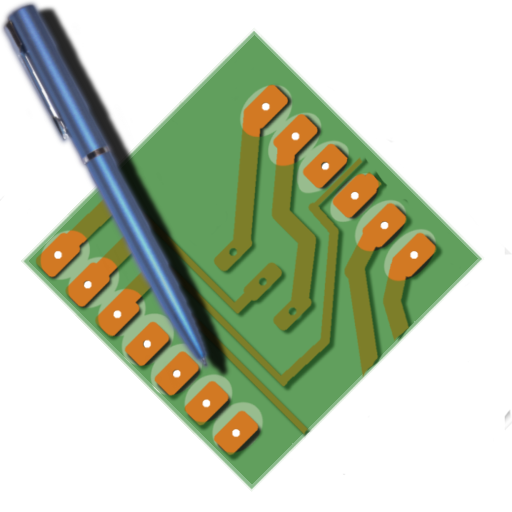
\includegraphics[width=.7\textwidth]{icona_fidocadj_a}
}

 \makeindex


\begin{document}
\pagenumbering{roman}

\pdfbookmark[1]{Front}{Front}
\maketitle 

\clearpage
\pdfbookmark[1]{Licence}{Licence}


\clearpage{} \pdfbookmark[1]{Licence}{Licence} This manual is covered
by the Creative Commons Public License version 2.5 or more recent.
The entire text of this licence is available at the address\\
 \href{http://creativecommons.org/licenses/by-nc-nd/3.0/}{http://creativecommons.org/licenses/by-nc-nd/3.0/}.

You are free to reproduce, diffuse, communicate or expose in public,
represent, execute and play this work at the following conditions:
\begin{description}
\item [{Attribution}] {You must attribute the work in the manner specified
by the author or licensor (but not in any way that suggests that they
endorse you or your use of the work).} 
\item [{Noncommercial}] {You may not use this work for commercial purposes.} 
\item [{No Derivative Works}] {You may not alter, transform, or build
upon this work.} 
\end{description}
Any of the above conditions can be waived if you get permission from
the copyright holder (Davide Bucci). \vfill{}


All commercial names, logo, trademarks cited in this work are registered
by their owners.

\begingroup %\let\clearpage\relax
%\let\cleardoublepage\relax
%\let\cleardoublepage\relax



\chapter*{Abstract}

\pdfbookmark[1]{Abstract}{Abstract}

This document is the FidoCadJ user manual. After a short
introduction describing the history and the birth of this software, we
describe the basic use of FidoCadJ. Our goal is to show how to draw
very simple electronic schematics and printed circuit boards.
The manual ends with a detailed description of the FidoCadJ format previously used by FidoCAD too. Finally, we give some hints about downloading and installing FidoCadJ using the most widespread operating systems: Linux, MacOSX and Windows.

This document presents only the program itself and the file format. It does not deal with the integration of FidoCadJ in websites, nor with the organization of the code and the aspects of development. Refer to the GitHub repository if you want to participate to the development!
\endgroup


\chapter*{Acknowledgements}

\pdfbookmark[1]{Aknowledgements}{Aknowledgements}

A number of people used this software since its first versions and
helped me by providing their advices. I thus want to thank the it.hobby.elettronica\index{it.hobby.elettronica}
newsgroup\index{newsgroup} participants for the very fruitful discussions we had together.

This software has been very carefully tested on Linux thanks to
Stefano Martini's patience. He was a very attentive alpha and beta
tester! I would like to thank Olaf Marzocchi and Emanuele Baggetta
for their tests on MacOSX.

I would like to thank ``F. Bertolazzi'' who has given very useful
advices about the usability of this software. He also assembled the
CadSoft Eagle\index{Eagle} compatibility library, useful to export
FidoCadJ drawings to Eagle. Many thanks to ``Celsius,'' who tested
the software functionalities for PCBs, as well as its libraries.
Thanks to Andrea D'Amore, too, for his advices concerning the FidoCadJ user interface on the Apple Macintosh. I would like to thank 
Roby IZ1CYN for the discussions about libraries and for having written 
section~\ref{installazione_linux} of this manual, dealing with its installation on Linux\index{Linux}.
Macintosh users can use FidoCadJ well integrated in the look of their operating system thanks to the Quaqua\index{Quaqua} look and feel, provided by Werner Randelshofer and more recently thanks to the VAqua7 look and feel.
Werner has also given useful advices about FidoCadJ's user interface: thanks for that!

Part of this manual has been translated to English by ``Pasu''. I would like to thank him for his hard work. I would like to thank Miles ``qhg007'' as well, for the careful check and very useful remarks.  

In April 2010, FidoCadJ has been integrated in the well known Italian web site \href{http://www.electroyou.it}{www.electroyou.it}. It now silently runs on the server and it automagically converts drawings posted on the forum.
I would like to express my gratitude to the admin Zeno Martini and webmaster Nicol� Martini and to all users of this site. They gave me a lot of very useful ideas about batch controlling FidoCadJ: a very promising path has been traced which deserves to be fully explored. FidoCadJ is also adopted on \href{http://www.matematicamente.it}{http://www.matematicamente.it}\index{http://www.matematicamente.it}. The FidoReadPHP project has been started in order to read and interpret FidoCadJ drawings on a PHP server, but it is unfortunately not actively maintained while I am writing those lines. It has been used by the popular \href{http://www.grix.it}{www.grix.it}\index{www.grix.it} website thanks to the efforts of Arniek, Sstrix and Stan. Many kudos to them!

Useful hints about FidoCadJ's website came from Federica Garin and Emanuele Baggetta. Sergio Juanez also greatly contributed to it, improving technical aspects and organization.

\chapter*{FidoCadJ License}

\pdfbookmark[1]{License FidoCadJ}{License FidoCadJ}

Copyright \copyright\ 2007-2020 the FidoCadJ development team. 

This software is free: you can redistribute it and/or modify it under
the terms of the GNU General Public License as published by the Free
Software Foundation, version 3 of the License.

This program is distributed in the hope that it will be useful, but
WITHOUT ANY WARRANTY; without even the implied warranty of MERCHANTABILITY
or FITNESS FOR A PARTICULAR PURPOSE. See the GNU General Public License
for more details.

You should have received a copy of the GNU General Public License
along with this program. If not, see \href{http://www.gnu.org/licenses/}{http://www.gnu.org/licenses/}.

\tableofcontents
\pdfbookmark[1]{Table of contents}{Table of contents}

\listoffigures
\pdfbookmark[1]{List of figures}{List of figures}

\begingroup
\let\clearpage\relax
\let\cleardoublepage\relax
\let\cleardoublepage\relax
\listoftables
\pdfbookmark[1]{Liste of tables}{Liste of tables}

\endgroup

\chapter{Introduction} \pagenumbering{arabic} In this chapter,
we will briefly introduce FidoCadJ. In particular, we will give a
description of the philosophy behind this software, as well as a brief
history of its development. 
If you need to install and run FidoCadJ, jump to appendix~\ref{specifics}, that   describes how to install FidoCadJ on the most widespread operating systems.

\section{FidoCadJ's philosophy}

FidoCAD\index{FidoCAD} (without the J at the end) was a vector
drawing software particularly suited for electrical schematics\index{electrical schematic} as well
as simple printed circuit boards\index{PCB}. It was employed by the italian Usenet community during the late 1990s.

It can still be freely downloaded (a Windows\index{Windows} version nationalized
in Italian language) from Lorenzo Lutti's page\index{Lorenzo Lutti}:

\href{http://www.enetsystems.com/~lorenzo/fidocad.asp}{http://www.enetsystems.com/\textasciitilde lorenzo/fidocad.asp}

The output files generated by FidoCAD was a very compact text code. This feature made it very easy to include drawings in text messages, such as those used in non-binary Usenet groups\index{Usenet group}.

Unfortunately, FidoCAD existed only in a Windows\index{Windows} version.
Linux users could run it using WInE\index{WInE}, but those relying on
other platforms like me (I use macOS) had to find a different solution.
I thus decided to give a small contribution to the community
by writing FidoCadJ (with the final J, this time). This editor is
written in pure Java\index{Java} and it is completely multi-platform.
FidoCadJ allows showing and modifying a drawing using the FidoCAD\index{FidoCAD}
file format. Nowadays, I am not alone anymore working on the project and FidoCadJ is a full-fledged and I dare to write successful Open Source project, with contributions coming from all over the world.

Whoever used FidoCAD\index{FidoCAD} in the past should become acquainted
with FidoCadJ very quickly, since many commands and procedures are
quite similar to the original application. FidoCadJ is almost completely compatible with the original FidoCAD, apart from a few details. The goal of a complete compatibility has been pursued until possible, but the needs of the new users have pushed towards some extensions to the original format.

Among the features offered by FidoCadJ and not present in the original
FidoCAD are the export possibilities offered. Since I am a \LaTeX{}
user, I decided to include an export feature for a number of vector
formats, including Encapsulated PostScript (\textsc{EPS}\index{EPS}) and scripts for the \textsc{PGF}\index{PGF} package. Of course, FidoCadJ can export towards the very well known \textsc{PDF}\index{PDF} format, with some limitations.

\section{History of FidoCadJ}

I have long been interested in electronic circuits. When I began following
several dedicated italian Usenet newsgroups\index{newsgroups}, I
noticed that many schematics were provided using the FidoCAD for Windows
format\index{FidoCAD}. This was much better than awkward ASCII drawings. Since
I do not use Windows, it was almost impossible
for me to look at them and I wanted to try to do something to solve
this problem. \marginpar{By the way, I think that it is better to
actively work at a solution rather than whining, because an operating system different from Windows lacks a particular software.}

The first thing I did towards the end of 2006 was to study the file format used by FidoCAD\index{FidoCAD} and write a Java\index{Java} applet called FidoReadJ\index{FidoReadJ}. It was able to parse the circuit and show it in a web page. Internet was different back then! To do that, I searched more or less everywhere (old posts, web pages), and did a lot of reverse engineering from existing FidoCAD files. I downloaded and studied the FidoCAD sources, too, written in a pretty clear C++ by Lorenzo Lutti.

I wrote the core of the applet about in March 2007. A few moths later,
the applet was on line and being tested by part of the community
gravitating around it.hobby.elettronica\index{it.hobby.elettronica}
and it.hobby.fai-da-te\index{it.hobby.fai-da-te}.%
\footnote{FidoReadJ\index{FidoReadJ} is still available today at the following address, in the unlikely possibility that your web browser still supports Java applets:\\
 \href{http://davbucci.chez-alice.fr/index.php?argument=elettronica/fidoreadj/fidoreadj.inc}{http://davbucci.chez-alice.fr/index.php?argument=elettronica/fidoreadj/fidoreadj.inc}.%
}

Since I had an interpreter\index{interpreter} of the FidoCAD format,
it was interesting to obtain a complete
editor\marginpar{To be honest, I made a first attempt at writing
a 2D vector drawing system around 1993.}. Much of the initial work was done in several steps, between January and July 2008: FidoCadJ
is not a port of FidoCAD for Windows, but it is
a new program, rewritten from scratch.

The choice of using Java\index{Java} is due to the fact that I currently use many different operating systems. Spending time
and energies on something which is not completely portable does not
appeal to me anymore. The effort of learning the Cocoa framework would
have probably given a better result on macOS, but it would have
made FidoCadJ completely non-portable. I am not a computer guy. The
time I spend to program is time taken away from my electronics interests.
In fact, especially at the beginning, the FidoCadJ code source showed that
I am not a very Java\index{Java} and object oriented programming\index{Object oriented programming}
purist and several solutions were
more practical than elegant. However, I tried to improve continuously the overall code quality FidoCadJ has been quite successfully compared to other Open Source projects\footnote{See for example \href{http://www.cs.usask.ca/~croy/papers/2013/RahmanStackOverflowTechReport.pdf}{Rahman, M. M., Roy, C. K., and Keivanloo, I. ``Subjective Evaluation of Software Quality Using Crowdsource Knowledge: An Exploratory Study''. Univ. of Saskatchewan, Department of Computer Science technical report 2013-01}}. Continuing in this way, static and dynamic analysis of the source code has been exploited to suggest where to refactor and improve the code organization.

What matters is the end user impressions while using the program,
more than the choice of a particular language. For this reason, I
am always listening to your suggestions, in order to understand how
to further develop this project. Java\index{Java}
may not the perfect choice or the solution to every problem. However
it has proven to be flexible enough for a tool like FidoCadJ.

% La parte interamente tradotta da Pasu comincia qui.

Without aiming for perfection and knowing the limits of my programming skills,
my intent is to make sure that FidoCadJ will NOT be another poor quality
application. For this reason any bug report or comment on the program's
usability will be more than welcome.

In November 2009, I opened a SourceForge\index{SourceForge} project dedicated to FidoCadJ. From this page, you could download all executables, manuals as well as the source code. Unfortunately, SourceForge progressively adopted some shady practices since 2013: advertisements with fake download buttons appeared everywhere and crap-ware added to installers for some projects. In 2015, the site was down for about 15 days: it become clear that it was time to change and we migrated the FidoCadJ project on GitHub\index{GitHub}. From August 2015, all development on FidoCadJ is done using Git: feel free to fork FidoCadJ and have a look at the sources. 

A deep refactoring of the existing code has been done by Kohta Ozaki and myself between 2013 and 2014, then gradually continued in 2015. This allowed to envisage the porting to Android platforms, which was made possible by the contribution of other people, in particular Dante Loi. Many other persons have given a hand in that moment. Even if the port was successful and a pre-release beta was ready and distributed, the work on Android unfortunately stalled since 2016.

If you want to help the community with FidoCadJ, do not worry: you do not need to be an expert Java programmer. You can for example translate the user interface or the manuals in a new language, check carefully the documentation for inconsistencies, typos and errors. FidoCadJ is currently available in Italian\index{Italian}, French\index{French}, English\index{English}, Spanish\index{Spanish}, German\index{German}, Chinese\index{Chinese}, Japanese\index{Japanese}, Greek\index{Greek}, Czech\index{Czech} and Dutch\index{Dutch}. Some translations may not be up-to-date anymore and require some work from the community. Search among the Issues on GitHub (with the ``translation'' tag) to see what is needed.
It is quite easy to translate menus and commands, so if you would
like to see FidoCadJ in your native language, please manifest yourself opening a new Issue on GitHub!
There is also work to be done to check the libraries (at least
the standard ones) and of course this manual.%
You can also work on the standard library\dots\
I consider that only half time I dedicate to FidoCadJ is in reality dedicated to the coding itself. The rest is spent answering questions from users, writing and improving the documentation and things like that.
On GitHub\index{GitHub}, you can participate to the discussions, as well as suggest improvements or give a bug report. Don't hesitate to participate:

\href{https://github.com/DarwinNE/FidoCadJ}{https://github.com/DarwinNE/FidoCadJ}

\section{FidoCadJ and the future}

In april 2010, I stumbled almost accidentally on a thread in a well known italian website \href{http://www.electroyou.it}{www.electroyou.it}. An user, Piercarlo Boletti, proposed to integrate a schematic capture tool directly inside the forum as something similar has already been done with \LaTeX\index{LaTeX@\LaTeX} equations. Since FidoCadJ was cited in his intervention, I inscribed myself to the forum and I offered to collaborate. I interacted with the very nice webmaster for a few days, and then the system was ready: a simple copy and paste in a post of the code describing the drawing, with a couple of tags. The forum runs automatically FidoCadJ on its servers and obtains an image, directly from the code. This image is then shown in the forum post, but its source code remains available. This way, who is reading the discussion does not need to have anything installed, but if one desires to change something, the code can be obtained with a few clicks.

Figure~\ref{fig_discussione_electroyou} shows part of one of my posts done on  \href{http://www.electroyou.it}{www.electroyou.it}. This system is so powerful and flexible that I have been the first to be astonished of the enthusiasm demonstrated by the users!\footnote{If you read Italian, here is an article I wrote:\\ \href{http://www.electroyou.it/darwinne/wiki/fidocadj}{http://www.electroyou.it/darwinne/wiki/fidocadj}  } FidoCadJ has shown to be useful also for drawings not directly related to electronics (see appendix \ref{chap_fidocadj_art} to see what I mean).
     
\begin{figure}
 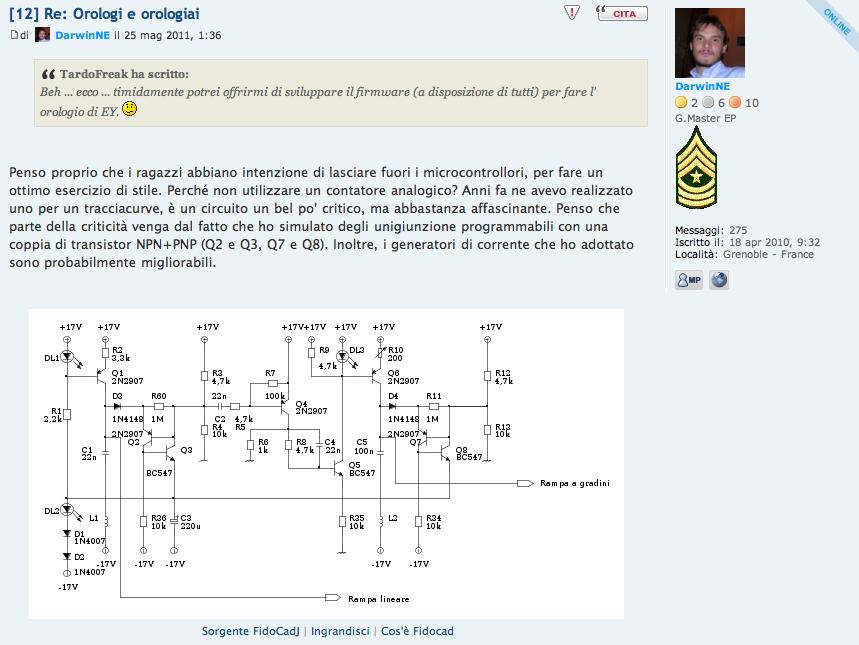
\includegraphics[width=\textwidth]{discussione_electroyou.png}
 \caption{Part of one of my posts on \href{http://www.electroyou.it}{www.electroyou.it}\index{www.electroyou.it}.
 With just one click you can zoom on the schematic. With a second one, you can obtain immediately the source code that you can paste on FidoCadJ to modify it.}
\label{fig_discussione_electroyou}
\end{figure}


The success that FidoCadJ has had on \href{http://www.electroyou.it}{www.electroyou.it}\index{www.electroyou.it} has stimulated some requests to implement a similar system on other platforms, and in particular on \href{http://www.grix.it}{www.grix.it}\index{www.grix.it}, another well known Italian electronics-dedicated website. FidoCadJ is also used by the \href{http://www.matematicamente.it/forum/viewtopic.php?f=38&t=121249}{Matematicamente}\index{Matematicamente} community.
In the case of \href{http://www.grix.it}{www.grix.it}\index{www.grix.it}, the server could not run a Java program and so the FidoReadPHP class has been written. It can be run on a PHP interpreter to obtain the images from the FidoCadJ source code.
The FidoReadPHP project is open source and it is available on SourceForge:

\href{https://sourceforge.net/projects/fidoreadphp/}{https://sourceforge.net/projects/fidoreadphp/}

The result is somewhat similar to what it has been obtained on \href{http://www.electroyou.it}{www.electroyou.it}, even if the graphical capabilities of PHP are quite limited in comparison with Java.
\footnote{Once again, if you read Italian, here is an article:\\
\href{http://www.grix.it/viewer.php?page=9335}{http://www.grix.it/viewer.php?page=9335}}
Figure~\ref{fig_fidocadj_grix3} shows an example of a drawing obtained with FidoReadPHP.

\begin{figure}
 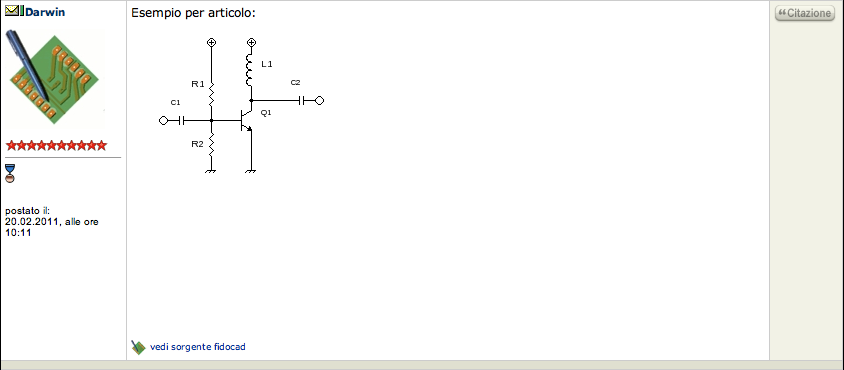
\includegraphics[width=\textwidth]{fidocadj_grix3.png}
 \caption{An example of a FidoCadJ drawing integrated in a \href{http://www.grix.it}{www.grix.it}\index{www.grix.it} forum post. You can obtain the source code of the drawing with just a mouse click.}
 \label{fig_fidocadj_grix3}
\end{figure}

I think that the future of FidoCadJ is not to become more complex, as a complete CAD for electronics. Probably, those possibilities of integration with discussion groups and forums deserve to be developed. Experience has shown that this is possible and the enthusiasm of the users has been tantalizing. 

\chapter{Drawing with FidoCadJ}

The use of FidoCadJ should be quite intuitive for those who already
used a vector drawing application\index{vector drawing}. A
screenshot of the program running on MacOSX\index{MacOSX} is shown
in Fig.~\ref{fig_fidocadj};\marginpar{Expert Mac-users will notice
that all the menus are at their own place!} A few details may be
different when running on other operating systems (for example
Fig.~\ref{fig_metal} shows the result with Look and Feel Metal\index{Metal}
on Sun/Oracle\index{Sun/Oracle}), but the philosophy remains the same. We will
see what the features of the program are, and its basic elements (the
primitives)\index{primitive} which compose a FidoCadJ drawing. %
\begin{figure}
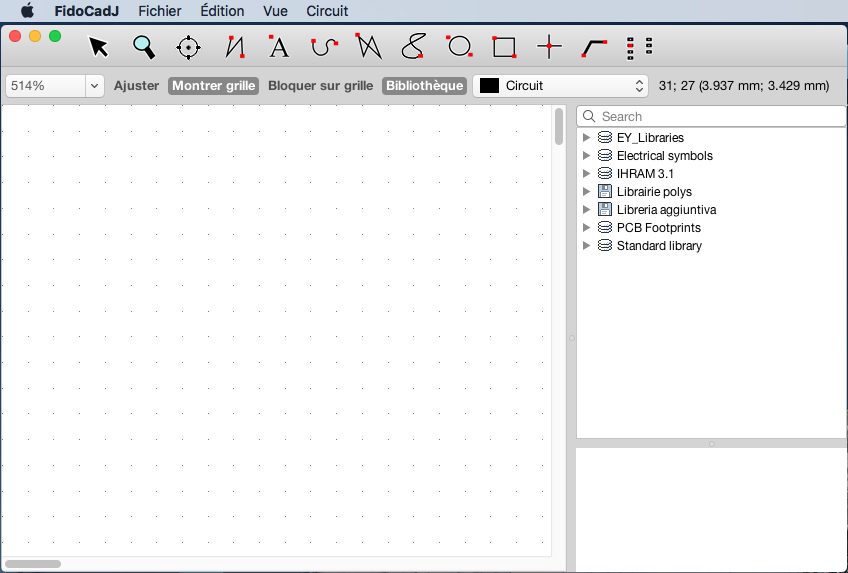
\includegraphics[width=1\textwidth]{fidocadj_macosx.png} 

\caption{A FidoCadJ session running on a vintage MacOSX Tiger\index{MacOSX}.
Appendix~\ref{specifics} describes the peculiarities of the version
specific for Macintosh\index{Macintosh}. More recent versions provide the quick search in the library, shown in figure~\ref{fig_ricerca}.}

\label{fig_fidocadj} 
\end{figure}

%
\begin{figure}
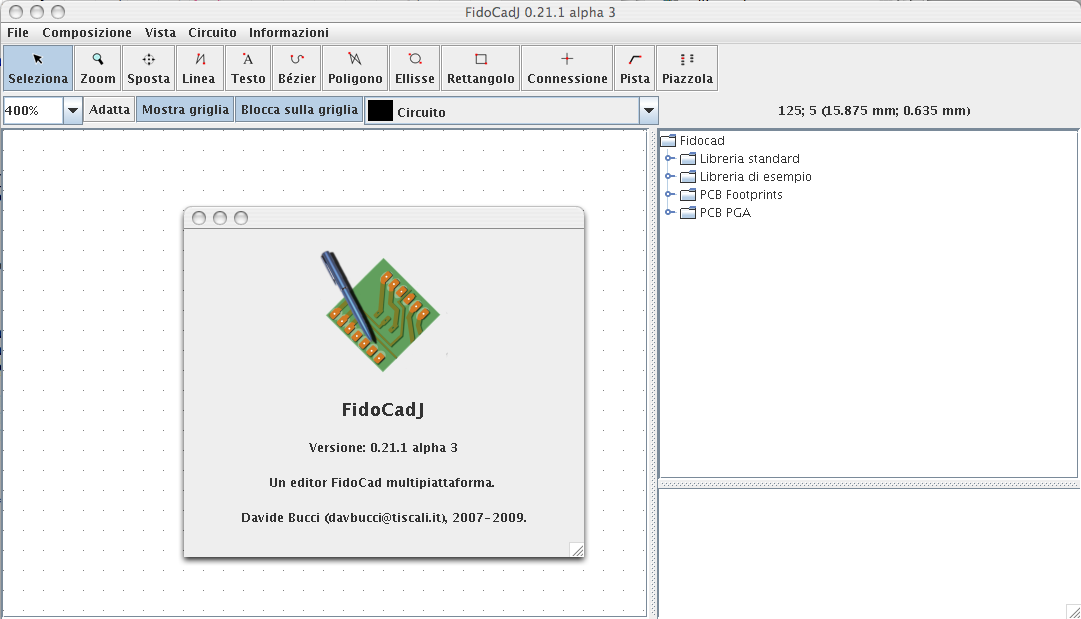
\includegraphics[width=1\textwidth]{fidocadj_metal.png} 

\caption{FidoCadJ with the Look and Feel Metal\index{Metal}.}


\label{fig_metal} 
\end{figure}

\section{Drawing Tools}

In the toolbar\index{toolbar} (on the top of the window), we can
find the most used features that allow the creation and the editing
of a drawing. Table~\ref{tab_comandi} shows a brief summary of the
functionalities and the commands and describes the possible actions.
You will notice that once a button is pressed, it will remain in that
position until another function from the toolbar will be selected.\marginpar{This
behavior is inspired to the old vacuum tube radios and to the switches
very fashionable in the '70s.} From the toolbar we can select which
drawing primitive\index{primitive} will be used.%
\footnote{For more information on the drawing elements, see~\ref{sec_primitive}.%
} On the right, a drop-down menu will show the current working layer
(see~\ref{sec_layer} for more information).

The command bar\index{command bar} can be partially customized. In
particular, we can choose whether we want to see the icon on each
button or the icon and its text description. Icons are also available
in two selectable formats. To change these settings we can select
the menu {}``File/Options''.%
\footnote{Except on MacOSX, where this item is found in the FidoCadJ's menu
and it is called {}``Preferences''.%
} Any change in the settings will be applied at the restart of the
application, since it is arguably something that we may want to change
every day. Figures \ref{fig_fidocadj} and \ref{fig_metal} show the
command bar (right below the window's title), configured to show text
and icons in their smallest version. On the second row, starting from
the left we can see the zoom settings and the buttons {}``Fit'',
{}``Show grid'' e {}``Snap to grid''. The first allows us to automatically
select the most suitable zoom settings in order to show the whole
drawing on the screen. The second toggles between visible and invisible
grid, while when we press the third button the elements added will
stick to the nearest step of the grid.
If you need to align carefully the elements, you may find useful to keep pressed \keyevidence{Alt}, while using the cursor keys.

%
\begin{table}
\centering \begin{tabular}{clp{0.6\textwidth}}
\toprule Key & Command  & Use\tabularnewline
\midrule
\keyevidence{A},\keyevidence{ESC} or \newline \keyevidence{space}  & \raisebox{-.2em}{
\includegraphics[width=1em]{icons/arrow}}
\textsc{Select}\index{selection}  & Selects one or more graphic elements. Press \keyevidence{Control}
(\keyevidence{Command} on MacOSX) for multiple selections
or to deselect only one element. Click and drag to select several
elements in an area. Press \keyevidence{R} to rotate the selected
elements. Press \keyevidence{S} to mirror the selected elements.
Double-click on an element to modify its properties.
\tabularnewline
 & \raisebox{-.2em}{
\includegraphics[width=1em,]{icons/magnifier}}
\textsc{Zoom}\index{zoom}  & Left-click to increase the level of zoom. Right-click to decrease
it.\tabularnewline
 & \raisebox{-.2em}{
\includegraphics[width=1em,]{icons/move}}
\textsc{Move}\index{move}  & Click on the drawing and move the mouse to move the drawing.\tabularnewline
\keyevidence{L}  & \raisebox{-.2em}{
\includegraphics[width=1em,]{icons/line}}
\textsc{Line}\index{line}  & Inserts a line or a series of lines. Press \keyevidence{Esc} or
double-click to terminate the insertion %\footnote{In FidoCadJ versions prior to 0.20.5, a right click would switch to the ``Select'' mode}
\tabularnewline
\keyevidence{T}  & \raisebox{-.2em}{
\includegraphics[width=1em,]{icons/text}}
\textsc{Text}\index{text}  & Inserts a text string.\tabularnewline
\keyevidence{B}  & \raisebox{-.2em}{
\includegraphics[width=1em,]{icons/bezier}}
\textsc{B�zier}\index{B�zier}  & Draws a B�zier curve\tabularnewline
\keyevidence{P}  & \raisebox{-.2em}{
\includegraphics[width=1em,]{icons/polygon}}
\textsc{Polyline}\index{polyline}  & Draws a polyline filled or empty. Double-click or press \keyevidence{Esc},
to terminate the insertion of new vertices.\tabularnewline
\keyevidence{K}
&
\raisebox{-.2em}{%

\includegraphics[width=1em]{icons/complexcurve}%
}
\textsc{Curve}\index{curve}
&
Open or closed natural cubic spline curve. Double click or press \keyevidence{Esc},  to terminate the insertion of new vertices.\tabularnewline

\keyevidence{E}  & \raisebox{-.2em}{
\includegraphics[width=1em,]{icons/ellipse}}
\textsc{Ellipse}\index{ellipse}  & Draws an ellipse filled or empty (hold \keyevidence{Control} or \keyevidence{Command} in MacOSX for a circle). \tabularnewline
\keyevidence{G}  & \raisebox{-.2em}{
\includegraphics[width=1em,]{icons/rectangle}}
\textsc{Rect.}\index{rectangle}  & Draws a rectangle filled or empty (hold \keyevidence{Control} or \keyevidence{Command} in MacOSX  for a square). \tabularnewline
\keyevidence{C}  & \raisebox{-.2em}{
\includegraphics[width=1em,]{icons/connection}}
\textsc{Junction}\index{junction}  & Inserts an electrical junction.\tabularnewline
\keyevidence{I}  & \raisebox{-.2em}{
\includegraphics[width=1em,]{icons/pcbline}}
\textsc{PCB track}\index{PCB track}  & Draws a PCB track. The default width can be modified through the dialog
accessed from the menu {}``File/Options''. \tabularnewline
\keyevidence{Z}  & \raisebox{-.2em}{
\includegraphics[width=1em,]{icons/pcbpad}}
\textsc{PCB pad}\index{PCB pad@\textsc{PCB }pad}  & Draws a PCB pad. The default dimensions can be modified through the
dialog accessed from the menu {}``File/Options''. \tabularnewline
\bottomrule  &  & \tabularnewline
\end{tabular}

\caption{Summary of the drawing commands available in FidoCadJ. The key shown
on the leftmost column allows their rapid selection using the keyboard.
A right click in one of the primitive placement modes allows us to
access the properties window.}


\label{tab_comandi} 
\end{table}


On the right are shown in a tree list the symbols \index{macro}
(also called macros) of the loaded libraries. To insert in the drawing
an element from the library, we only need to select it from the list
an click on the drawing. FidoCAD\index{FidoCAD} libraries include
all standard symbols used in electrical schematics\index{electrical schematic} and a wide selection of footprints\index{PCB!footprint} for drawing PCBs.

You can also do quick research\index{Quick research} inside the libraries charged in FidoCadJ. You just need to type something in the text field which appears just over the tree representing the installed libraries (have a look to figure~\ref{fig_ricerca}). 
By typing return, you can navigate through the results.

\begin{figure}
\centering
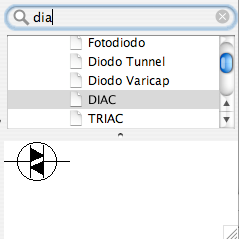
\includegraphics[width=.4\textwidth]{ricerca}
\caption{The quick search function in the installed libraries.}
\label{fig_ricerca}
\end{figure}
%
\begin{figure}
\centering 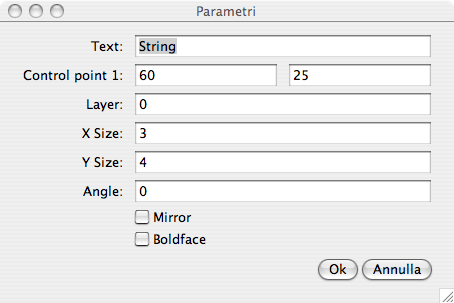
\includegraphics[width=0.7\textwidth,]{param_testo} 

\caption{Dialog for the text's parameters in a FidoCadJ drawing. The operating system is Mac OS X Yosemite (10.10.4) in French.}

\label{fig_param_testo} 
\end{figure}


Figure~\ref{fig_param_testo} shows an example of what we can obtain
by double-clicking, in selection mode\index{selection}, on a drawing
element (in this case a text string). Within this window it is possible
to modify all the parameters (coordinates, rotation\dots) of any
drawing element. The aspect of this window will change because the
information that can be modified will depend on the selected element.

\section{A simple schematic}

As an example of use of this application, we will show how to draw
the simple electrical schematic of figure~\ref{fig_schema}. %
\begin{figure}
\centering %\includegraphics[width=.5\textwidth]{schema}
\begin{pgfpicture}{0cm}{0cm}{125pt}{111pt}
% Created by FidoCadJ ver. 0.21, export filter by Davide Bucci
\pgfsetxvec{\pgfpoint{1pt}{0pt}}
\pgfsetyvec{\pgfpoint{0pt}{1pt}}
\pgfsetlinewidth{0.33pt}
\pgfsetroundjoin 
\pgftranslateto{\pgfxy(0,111)}
\begin{pgfmagnify}{1}{-1}
% Layer color definitions
\definecolor{layer0}{rgb}{0.0,0.0,0.0}
\definecolor{layer1}{rgb}{0.0,0.0,0.5}
\definecolor{layer2}{rgb}{1.0,0.0,0.0}
\definecolor{layer3}{rgb}{0.0,0.5,0.5}
\definecolor{layer4}{rgb}{1.0,0.78,0.0}
\definecolor{layer5}{rgb}{1.0,0.78,0.0}
\definecolor{layer6}{rgb}{1.0,0.78,0.0}
\definecolor{layer7}{rgb}{1.0,0.78,0.0}
\definecolor{layer8}{rgb}{1.0,0.78,0.0}
\definecolor{layer9}{rgb}{1.0,0.78,0.0}
\definecolor{layer10}{rgb}{1.0,0.78,0.0}
\definecolor{layer11}{rgb}{1.0,0.78,0.0}
\definecolor{layer12}{rgb}{1.0,0.78,0.0}
\definecolor{layer13}{rgb}{1.0,0.78,0.0}
\definecolor{layer14}{rgb}{1.0,0.78,0.0}
\definecolor{layer15}{rgb}{1.0,0.78,0.0}
% End of color definitions
\color{layer0}
\pgfline{\pgfxy(100,67)}{\pgfxy(105,70)}
\pgfline{\pgfxy(90,65)}{\pgfxy(100,65)}
\pgfline{\pgfxy(100,60)}{\pgfxy(100,70)}
\pgfline{\pgfxy(105,60)}{\pgfxy(105,55)}
\pgfline{\pgfxy(100,63)}{\pgfxy(105,60)}
\pgfline{\pgfxy(105,70)}{\pgfxy(105,75)}
\pgfmoveto{\pgfxy(103,70)}
\pgflineto{\pgfxy(104,68)}
\pgflineto{\pgfxy(105,70)}
\pgfclosepath 
\pgffill 
\begin{pgfmagnify}{1}{-1}
\pgfputat{\pgfxy(110,-55)}{\pgfbox[left,top]{\footnotesize{Q1B}}}
\end{pgfmagnify}
\begin{pgfmagnify}{1}{-1}
\pgfputat{\pgfxy(110,-65)}{\pgfbox[left,top]{\footnotesize{LM394}}}
\end{pgfmagnify}
\pgfline{\pgfxy(40,67)}{\pgfxy(35,70)}
\pgfline{\pgfxy(50,65)}{\pgfxy(40,65)}
\pgfline{\pgfxy(40,60)}{\pgfxy(40,70)}
\pgfline{\pgfxy(35,60)}{\pgfxy(35,55)}
\pgfline{\pgfxy(40,63)}{\pgfxy(35,60)}
\pgfline{\pgfxy(35,70)}{\pgfxy(35,75)}
\pgfmoveto{\pgfxy(37,70)}
\pgflineto{\pgfxy(36,68)}
\pgflineto{\pgfxy(35,70)}
\pgfclosepath 
\pgffill 
\begin{pgfmagnify}{1}{-1}
\pgfputat{\pgfxy(10,-55)}{\pgfbox[left,top]{\footnotesize{Q1A}}}
\end{pgfmagnify}
\begin{pgfmagnify}{1}{-1}
\pgfputat{\pgfxy(0,-65)}{\pgfbox[left,top]{\footnotesize{LM394}}}
\end{pgfmagnify}
\pgfline{\pgfxy(50,65)}{\pgfxy(90,65)}
\pgfline{\pgfxy(35,75)}{\pgfxy(35,95)}
\pgfline{\pgfxy(105,75)}{\pgfxy(105,95)}
\pgfline{\pgfxy(35,40)}{\pgfxy(35,55)}
\pgfline{\pgfxy(35,30)}{\pgfxy(35,32)}
\pgfmoveto{\pgfxy(36,32)}
\pgflineto{\pgfxy(34,32)}
\pgflineto{\pgfxy(34,38)}
\pgflineto{\pgfxy(36,38)}
\pgfclosepath 
\pgfqstroke 
\pgfline{\pgfxy(35,38)}{\pgfxy(35,40)}
\begin{pgfmagnify}{1}{-1}
\pgfputat{\pgfxy(45,-40)}{\pgfbox[left,top]{}}
\end{pgfmagnify}
\begin{pgfmagnify}{1}{-1}
\pgfputat{\pgfxy(45,-35)}{\pgfbox[left,top]{}}
\end{pgfmagnify}
\pgfline{\pgfxy(35,15)}{\pgfxy(35,30)}
\pgfline{\pgfxy(25,15)}{\pgfxy(35,15)}
\pgfline{\pgfxy(25,15)}{\pgfxy(23,15)}
\pgfellipse[stroke]{\pgfxy(21.0,15.0)}{\pgfxy(2.0,0)}{\pgfxy(0,2.0)}
\pgfline{\pgfxy(22,15)}{\pgfxy(20,15)}
\pgfline{\pgfxy(21,16)}{\pgfxy(21,14)}
\begin{pgfmagnify}{1}{-1}
\pgfputat{\pgfxy(35,-25)}{\pgfbox[left,top]{}}
\end{pgfmagnify}
\begin{pgfmagnify}{1}{-1}
\pgfputat{\pgfxy(35,-20)}{\pgfbox[left,top]{}}
\end{pgfmagnify}
\pgfline{\pgfxy(35,50)}{\pgfxy(55,50)}
\pgfline{\pgfxy(55,50)}{\pgfxy(55,65)}
\pgfcircle[fill]{\pgfxy(55,65)}{1pt}\pgfcircle[fill]{\pgfxy(35,50)}{1pt}\pgfline{\pgfxy(105,45)}{\pgfxy(105,55)}
\pgfline{\pgfxy(105,35)}{\pgfxy(105,40)}
\pgfline{\pgfxy(105,25)}{\pgfxy(105,30)}
\pgfline{\pgfxy(35,95)}{\pgfxy(35,100)}
\pgfline{\pgfxy(32,100)}{\pgfxy(38,100)}
\pgfline{\pgfxy(33,101)}{\pgfxy(37,101)}
\pgfline{\pgfxy(34,102)}{\pgfxy(36,102)}
\begin{pgfmagnify}{1}{-1}
\pgfputat{\pgfxy(45,-105)}{\pgfbox[left,top]{}}
\end{pgfmagnify}
\begin{pgfmagnify}{1}{-1}
\pgfputat{\pgfxy(45,-100)}{\pgfbox[left,top]{}}
\end{pgfmagnify}
\pgfline{\pgfxy(105,95)}{\pgfxy(105,100)}
\pgfline{\pgfxy(102,100)}{\pgfxy(108,100)}
\pgfline{\pgfxy(103,101)}{\pgfxy(107,101)}
\pgfline{\pgfxy(104,102)}{\pgfxy(106,102)}
\begin{pgfmagnify}{1}{-1}
\pgfputat{\pgfxy(115,-105)}{\pgfbox[left,top]{}}
\end{pgfmagnify}
\begin{pgfmagnify}{1}{-1}
\pgfputat{\pgfxy(115,-100)}{\pgfbox[left,top]{}}
\end{pgfmagnify}
\begin{pgfmagnify}{1}{-1}
\pgfputat{\pgfxy(40,-30)}{\pgfbox[left,top]{\footnotesize{10 k}}}
\end{pgfmagnify}
\begin{pgfmagnify}{1}{-1}
\pgfputat{\pgfxy(110,-45)}{\pgfbox[left,top]{\footnotesize{I}}}
\end{pgfmagnify}
\pgfmoveto{\pgfxy(105,55)}
\pgflineto{\pgfxy(104,53)}
\pgflineto{\pgfxy(106,53)}
\pgfclosepath 
\pgffill 
\pgfline{\pgfxy(105,55)}{\pgfxy(105,50)}
\begin{pgfmagnify}{1}{-1}
\pgfputat{\pgfxy(115,-60)}{\pgfbox[left,top]{}}
\end{pgfmagnify}
\begin{pgfmagnify}{1}{-1}
\pgfputat{\pgfxy(115,-55)}{\pgfbox[left,top]{}}
\end{pgfmagnify}
\end{pgfmagnify}
\end{pgfpicture} 

\caption{The reference schematic: a current mirror made with NPN transistors.}


\label{fig_schema} 
\end{figure}


Once FidoCadJ is running, let us create a new drawing from the menu
{}``File/New''.

We will then start by placing in the drawing area the symbols for
the two transistors\index{transistor}, around which our schematic
is built. To do so, we will need the macros contained in the standard
library\index{standard library}, which is loaded by default and is
found on the right-hand side of the screen. The macro that we will
use is called {}``NPN transistor'' and is included in the {}``Diodes
and transistors'' category of the {}``Standard library''. By clicking
on the element's name to select the desired macro\index{macro}, it
will then be possible to place it anywhere in the drawing (FidoCadJ shows a preview), by clicking
a second time on the desired location. We should now be at the stage
similar to the one shown in figure ~\ref{fig_fidocadj_fase1}.

%
\begin{figure}
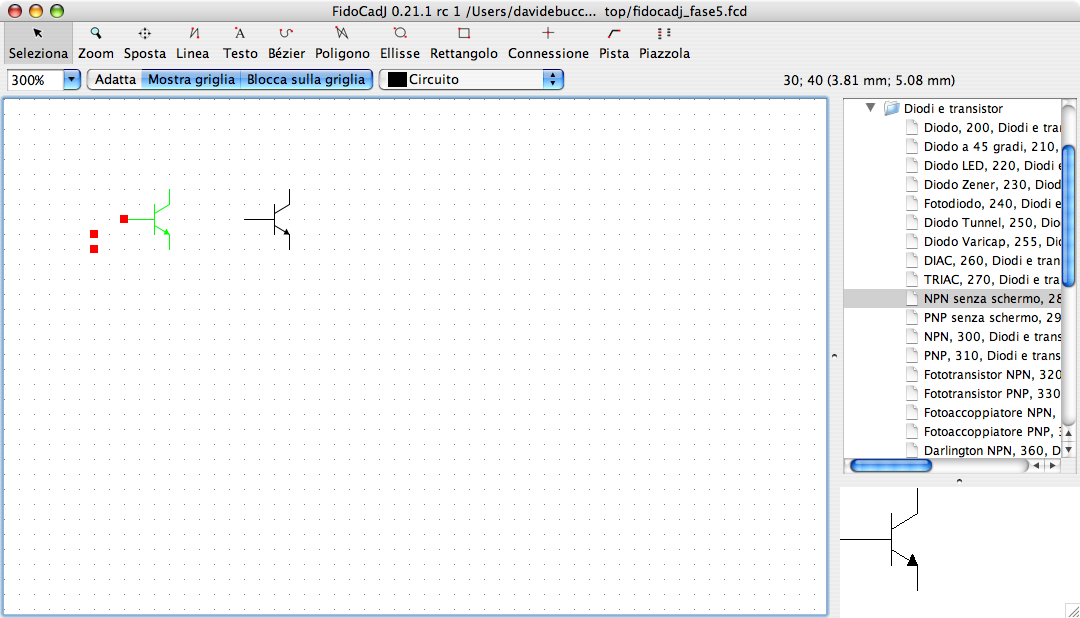
\includegraphics[width=1\textwidth,]{fidocadj_fase1} 

\caption{We start by drawing a couple of transistors.}


\label{fig_fidocadj_fase1} 
\end{figure}


We may notice that the bipolar transistor on the left is not correctly
oriented. To fix the problem is sufficient to click on {}``Select'',
from the toolbar, select the transistor (which will be highlighted
in green, with three control points\index{control point} identified
by small red squares) and then press \keyevidence{S} to obtain
its mirrored version. You may also press \keyevidence{S} when you have selected the symbol in the libraries and you are about to position it in the drawing. We will thus obtain a result similar to the
one shown in figure~\ref{fig_fidocadj_fase2}.

%
\begin{figure}
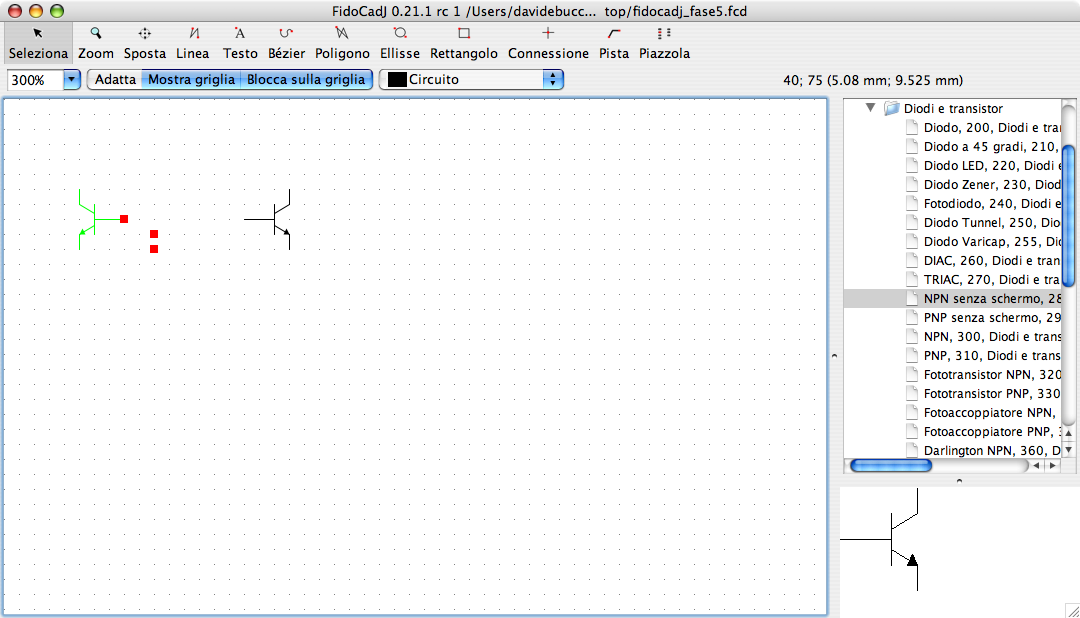
\includegraphics[width=1\textwidth,]{fidocadj_fase2} 

\caption{Select and mirror with \keyevidence{S} the transistor on the left.}


\label{fig_fidocadj_fase2} 
\end{figure}


By using the tool {}``Line'' from the toolbar\index{toolbar}, we
will be able to make a few electrical connections, until we will realize
that we started our drawing to close to the edges of the drawing area.
The issue can be easily fixed by selecting the whole drawing: in {}``Select''
mode, we can click on the upper left corner of the drawing and, holding
the left button of the mouse pressed, drag the cursor up to the lower
right corner. A rectangle with a green contour will appear to indicate
that we are trying to select all the elements included in it. Since
we want to move everything we have drawn so far, we will have to select
them all first(see figure~\ref{fig_fidocadj_fase3}). Now, still
in select mode, we can click on any selected element to drag the selection
to the desired position.

%
\begin{figure}
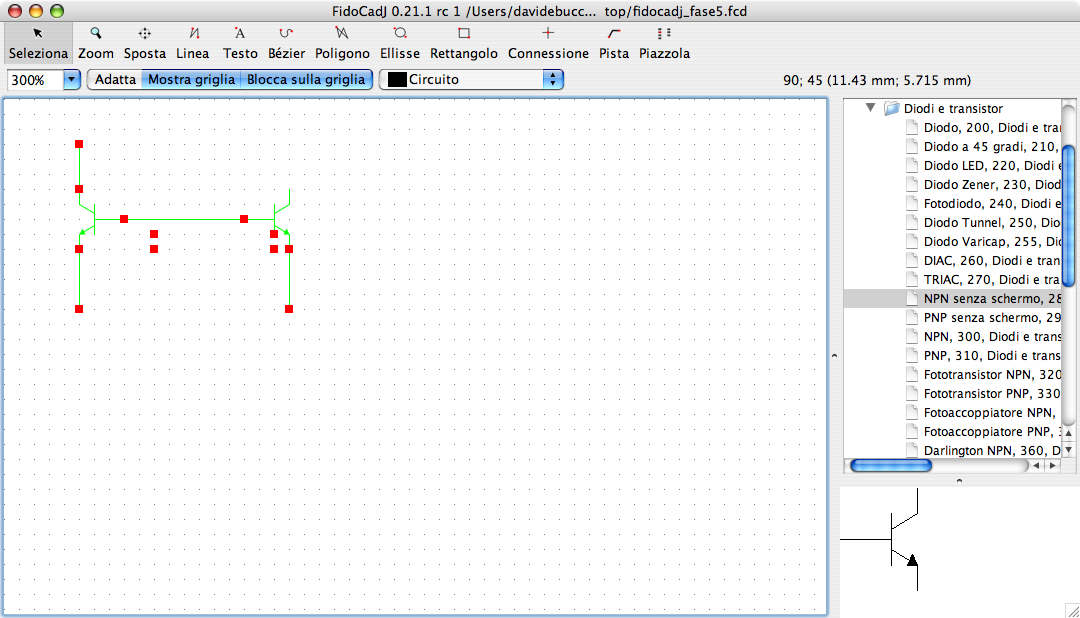
\includegraphics[width=1\textwidth,]{fidocadj_fase3} 

\caption{We are too close to the top edge of the sheet: let's select the whole
drawing and move it toward the centre.}


\label{fig_fidocadj_fase3} 
\end{figure}


We can then continue placing the other parts of the circuit, in particular
a resistor\index{resistor} (Standard Library/Discrete devices/Resistor)
and the label for the positive power supply (Standard Library/Basic symbols/Terminal +). We will need to rotate the latter in order to
place in the desired position. Again, we can select it and press \keyevidence{R}
until we will obtain the desired result. We should now have a screen
similar to the one in figure~\ref{fig_fidocadj_fase4}.

%
\begin{figure}
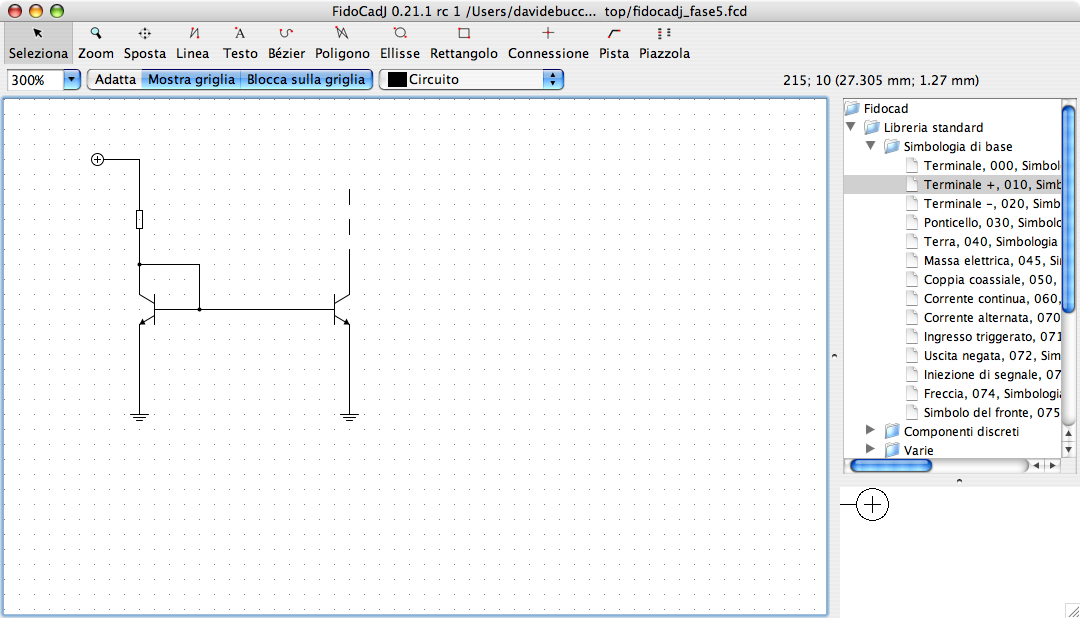
\includegraphics[width=1\textwidth,]{fidocadj_fase4} 

\caption{The circuit almost completed.}


\label{fig_fidocadj_fase4} 
\end{figure}


To complete the schematic we only need to add the text strings and
the arrow to indicate the direction of the current. For the latter
there is a macro called {}``Arrow'', contained in {}``Standard library/Basic symbols''. To place the text, we can press the
button {}``Text''\index{text} from the toolbar e click in the drawing
area on the desired position. As the default text {}``String'' will
be introduced, we will need to modify its characteristics by double-clicking
in select mode (see figure~\ref{fig_param_testo}). The transistor's
part number and name used (it is actually a transistor matched pair
in our example) are specified in the fields {}``Name'' and {}``Value''
which are accessed in select mode by double-clicking on the macro.%
\footnote{The feature which allows us to add a name and a value to a macro or
a component's symbol is actually an extension introduced with FidoCadJ
\index{FidoCadJ extension} not present in the original FidoCAD\index{FidoCAD}.
See section~\ref{FCJ_extension} for more information on compatibility.%
} The suggested dimension to work with electrical circuits is 4 units
in vertical and 3 units in horizontal. The complete circuit is shown
in figure~\ref{fig_fidocadj_fase5}.

%
\begin{figure}
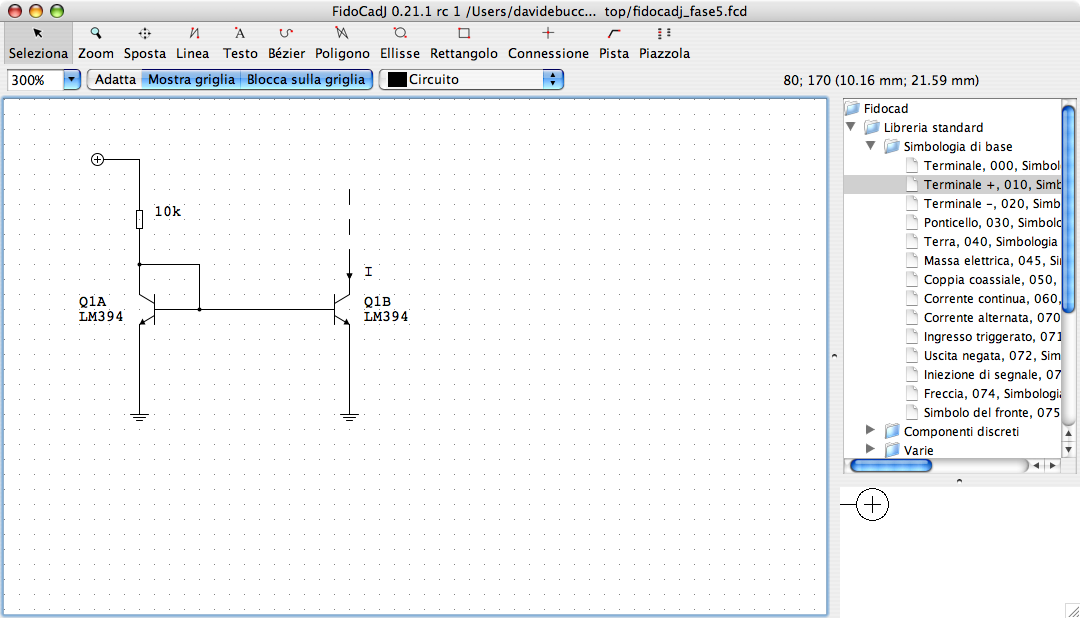
\includegraphics[width=1\textwidth,]{fidocadj_fase5} 

\caption{The final circuit.}


\label{fig_fidocadj_fase5} 
\end{figure}


As a curiosity, this is how the code\index{code} which describes
the circuit of our example looks like. To access this code, it is
sufficient to select {}``Insert Circuit'' from the menu {}``Circuit''.
We are now ready to copy and paste our circuit on an e-mail message\index{e-mail}, in a newsgroup\index{newsgroup}, or in a forum\index{forum}.
\begin{lstlisting}
[FIDOCAD]
MC 95 65 0 0 280
FCJ
TY 115 60 4 3 0 0 0 * Q1B
TY 115 65 4 3 0 0 0 * LM394
MC 55 65 0 1 280
FCJ
TY 20 60 4 3 0 0 0 * Q1A
TY 20 65 4 3 0 0 0 * LM394
LI 55 65 95 65 0
LI 40 75 40 95 0
LI 110 75 110 95 0
LI 40 40 40 55 0
MC 40 30 0 0 115
LI 40 15 40 30 0
LI 30 15 40 15 0
MC 30 15 2 0 010
LI 40 50 60 50 0
LI 60 50 60 65 0
SA 60 65 0
SA 40 50 0
LI 110 45 110 55 0
LI 110 35 110 40 0
LI 110 25 110 30 0
MC 40 95 0 0 040
MC 110 95 0 0 040
TY 45 30 4 3 0 0 0 * 10 k
TY 115 50 4 3 0 0 0 * I
MC 110 50 1 0 074
\end{lstlisting} 
If you are interested in the export format
used by FidoCAD, there is a detailed description on chapter~\ref{chap_formato}.

However, there is no need to use the {}``Insert circuit'' dialog;
we can simply select the entire drawing, copy it (by selecting ``edit/copy''
or by pressing \keyevidence{Ctrl+C} ) and paste it onto the message
we are writing and the code will be added automatically\index{code}.

Depending on the current settings, FidoCadJ can apply or not a diagonal shift\index{diagonal shift} to the copied elements. The $x$ and $y$ width and height are equal to the grid pitch. The default behaviour is to proceed in such a way, in order to differentiate the pasted elements from the original ones. Since in some situations this can be problematic, the settings can be changed in the ``Options''.


\section{The layers}

\label{sec_layer} A way to picture a layer\index{layer} is that
of a drawing made on acetate sheets. The final drawing will be given
by the combination of all the layers, which will be superposed like
acetates. Every layer is characterized by a different color and can
be visible or hidden. This approach is common to many CAD\index{CAD}
packages, as it allows an easy representation and management of different
parts of the drawing that will be superposed, as for example in a
PCB design\index{PCB}.

FidoCadJ allows up to 16 layers, numbered from 0 to 15. Conventionally,
some of the layers have a specific purpose. In particular, layer zero
is used for electrical schematics\index{electrical schematic}, layer
1 for the copper soldering side\index{soldering}, layer 2 for the
copper components side and layer 3 for the silk-screen\index{silk-screen}.
The remaining layers do not have any pre-defined purpose and can be
used freely. Name and color\index{colour} of every layer can be
specified using the menu {}``View/Layer''. From the same menu we
can also select the layers that we want to see on screen or that we
want to print.

The layers' ordering is important, as layer with a lower number will
be drawn first. That is, drawings on successive layers may cover the
ones on lower layers.


\section{The grid}

The logic unit\index{logic unit} in FidoCadJ is 5 mils (127 micron)
and ``half units'' are not allowed, meaning that the
coordinates of any graphic element must be integer numbers. This allows
us to obtain a resolution\index{resolution} sufficiently fine to
draw an electrical schematic and the majority of PCBs. However, for
ease of drawing, the application allows us to set a coarser grid and
force the mouse to align with the nearest point of the grid\index{grid}.
To enable this functionality there are two buttons, {}``Show Grid''
and {}``Snap'', which allow toggling between visible/hidden grid
and force the mouse cursor on the grid or let it move freely, respectively.
The grid step can be chosen through a dialog window that can be accessed
from the menu ``File/Options''.


\section{A simple PCB}
\marginpar{The reader
will find his way through: a few scribbles made with paper and pencil
(and a lot of erasers) will result in time saved by obtaining a clear
idea to be developed with the use of the computer.} 
To practice what we learnt so far, we will see how to design a simple
PCB. Unlike other software for electronic CAD which are very
powerful but sometimes quite hard to manage, FidoCadJ provides in
practice an electronic version of the good old R41 transfers\index{R41 transfers}, or the tape on mylar sheets.
Obviously, working on a computer allows us to benefit from all the
flexibility offered by the machine.

It must be noted that the design of a PCB\index{PCB}, especially
if this is a complex one, is not an easy task.  The autoplacer\index{autoplacer}
and the autorouter\index{autorouter} features promise miracles on
the publicity flyers from major CAD companies. There is no doubt that
these are still a tasks where the user's experience still plays an
important role. FidoCadJ constitutes a very immediate and fast way
to draw small PCBs on a DIY scale. We will see here how to draw a
very simple, yet complete, one.

I would suggest to start with a clear idea of where to place each
component and how to draw all the tracks so that they will cross each
other as less as possible\index{crossing of tracks}.

Here we will cheat a little and we will start from the result we want
to obtain, as shown in figure~\ref{fig_amplificateur}. It is a simple
common-emitter amplifier built around an NPN transistor, type BC547
or similar. It will be useful to think of the board as it was transparent,
by looking from the components side. For this purpose the silk-screen\index{silk-screen}
with the components drawing will be very useful, although probably
we do not want to print it out onto the actual board for a DIY project.

%
\begin{figure}
\centering 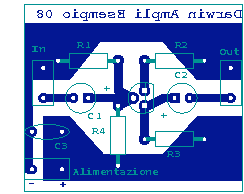
\includegraphics[width=0.5\textwidth]{amplificateur} 

\caption{A very simple amplifier stage using an NPN transistor connected in
a common emitter configuration.}


\label{fig_amplificateur} 
\end{figure}

The first thing I would suggest to do is to place all the components
as best as possible. In our example these would be the transistor
(from the library {}``PCB footprints/3 terminals semiconductors/TO92''),
the resistors ({}``PCB footprints/Resistors/Resistor 1/4 W 0,4 i''),
and the electrolytic capacitors ({}``PCB footprints/Electrolytic capacitor/Vert. diam. 5 mm 2.5 mm pitch''). In order to delimitate
the board, it may be useful to place an empty rectangle on the silk-screen
layer (layer No.~3). To do so we can use the \emph{rectangle} primitive\index{rectangle}
making sure that we selected the appropriate layer first. We should
get a result similar to the one shown in figure~\ref{fig_amplificateur_phase1}.%

%
\begin{figure}
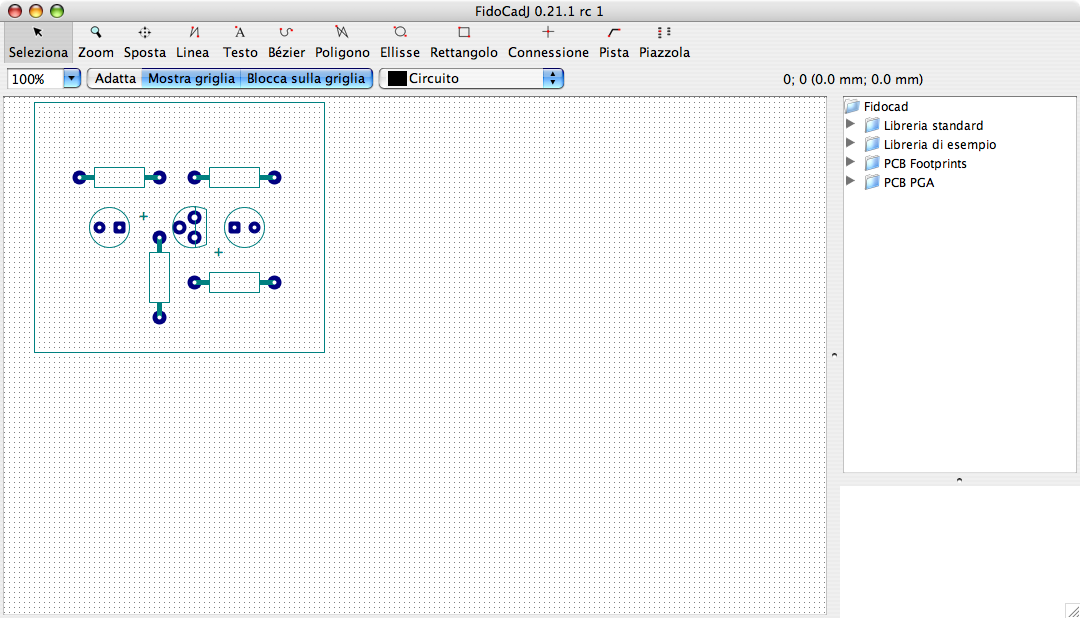
\includegraphics[width=1\textwidth]{amplificateur_phase1} 

\caption{The most important devices are placed on the board.}


\label{fig_amplificateur_phase1} 
\end{figure}


We can then introduce the copper areas which will provide the positive
and negative power supply. These are specified by drawing a polygon\index{polygon}
(using the \emph{poly line} primitive) and double clicking near its border 
in selection mode\index{selection mode} to tell FidoCadJ
(through dialog box) that we want a filled polygon. Before placing
the polygon, make sure that the current layer\index{layer} is the
one where we want to place the copper area (layer No~1, or copper
solder side). The use of a filled area for the power supply lines
may be useful to ensure that these connections will have a low stray
inductance. We should be able to reproduce the result shown in figure~\ref{fig_amplificateur_phase2}.

%
\begin{figure}
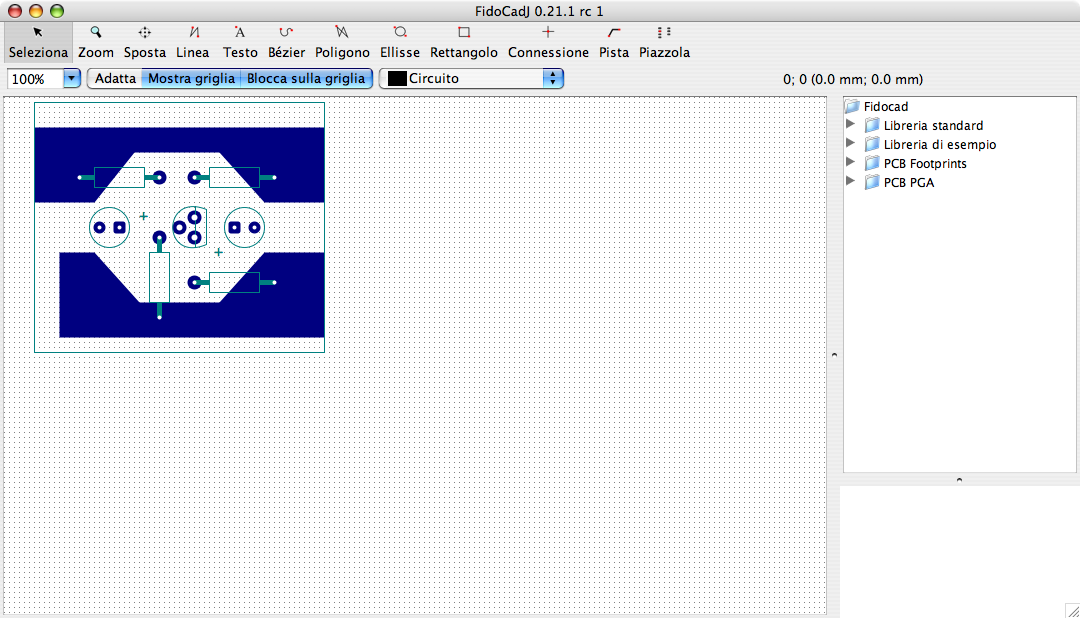
\includegraphics[width=1\textwidth]{amplificateur_phase2} 

\caption{Added the power supply connections using polygonal lines\index{polygon}.}


\label{fig_amplificateur_phase2} 
\end{figure}


To complete the electrical connections we can use the \emph{PCB line}
primitive\index{PCB line}. I chose a track thickness of 10 units
(1.27~mm), which helps the soldering process. %
\begin{figure}
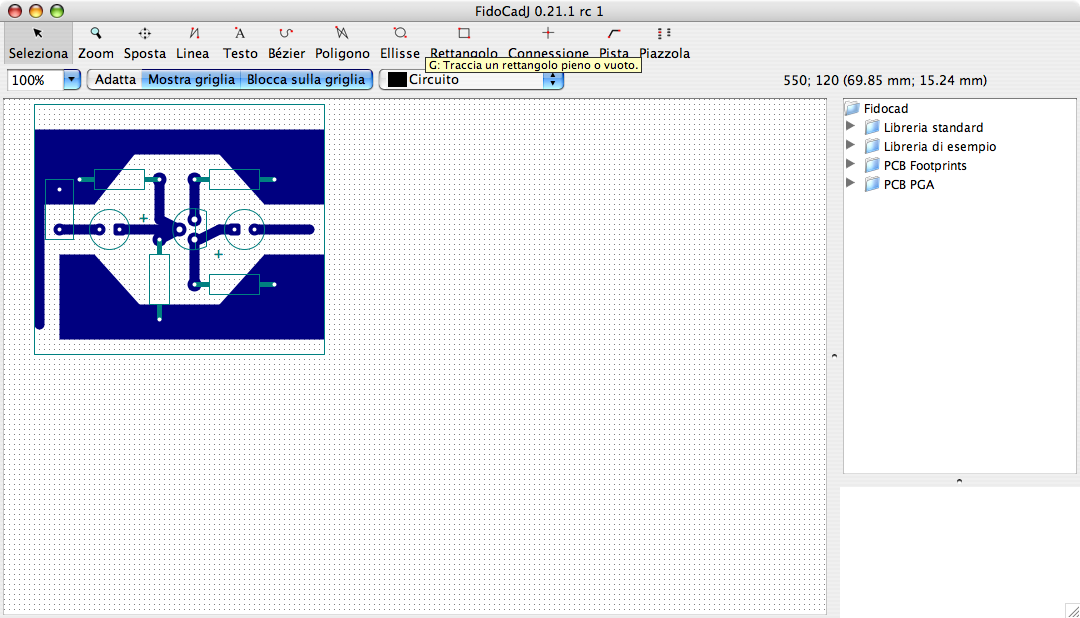
\includegraphics[width=1\textwidth]{amplificateur_phase3} 

\caption{Added the remaining connections PCB tracks\index{PCB track}.}


\label{fig_amplificateur_phase3} 
\end{figure}


We realize that we need a few connectors: one for the input, one for
the output and one for the power supply. We can use the footprint
designed for a polyester capacitor.  It will probably have the right dimensions. Let's
not forget that FidoCadJ is thought as a replacement for the transfers\index{R41 transfers}\dots

We can also place a ``$+$'' and a ``$-$'' on the copper layer and
place a ceramic capacitor in parallel with the power supply. \marginpar{Be careful with the
track widths: something that looks like a motor-way on the screen will
probably be a track so thin that will detach from the board during
the soldering.}
Let us
put the writing on the top side as well. To write on the copper layer,
after selecting the proper layer it will also be necessary to mirror
all the writings\index{writings mirroring}. This is easily done within
the usual properties dialog accessed by double-clicking on the string
we want to modify when we are in selection mode. It will need a few
tries to obtain the right dimensions for the characters. To give an
idea it is useful to have a ratio of 3/4 between the horizontal and
the vertical dimensions of the characters\index{characters dimension}.
Figure~\ref{fig_amplificateur_phase4} shows the result obtained
using 11 units for the horizontal and 18 units for the vertical dimension
of the text.

%
\begin{figure}
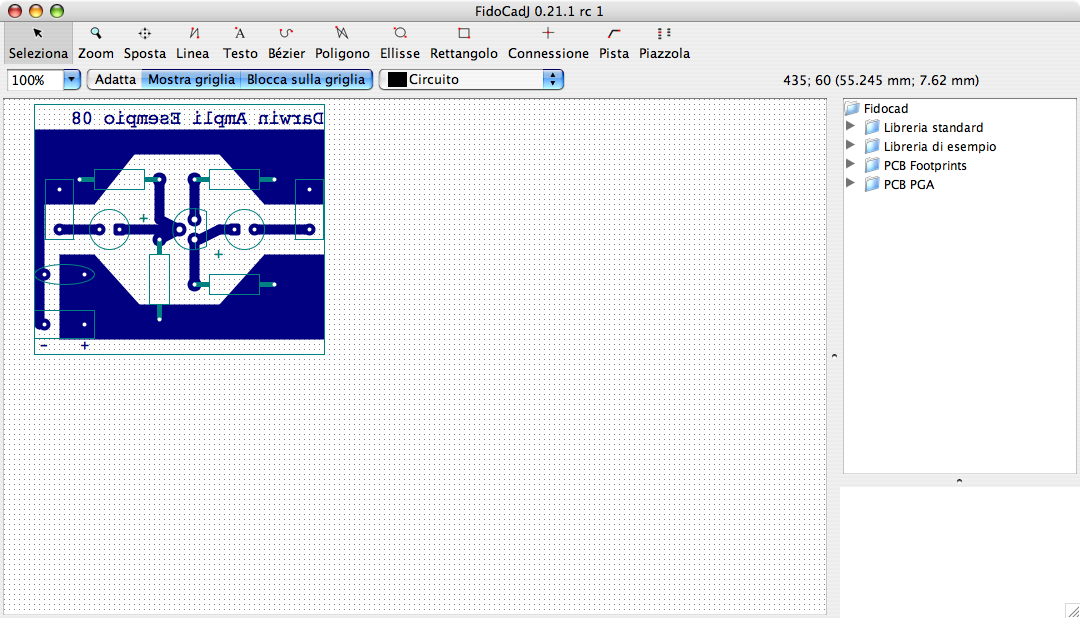
\includegraphics[width=1\textwidth]{amplificateur_phase4} 

\caption{The PCB almost completed\index{PCB}.}


\label{fig_amplificateur_phase4} 
\end{figure}


At this stage the only thing missing is the text with the name of
each component, that can be placed on layer 3 (silk-screen). The program
with the PCB completed is shown in Figure~\ref{fig_amplificateur_complet}.

%
\begin{figure}
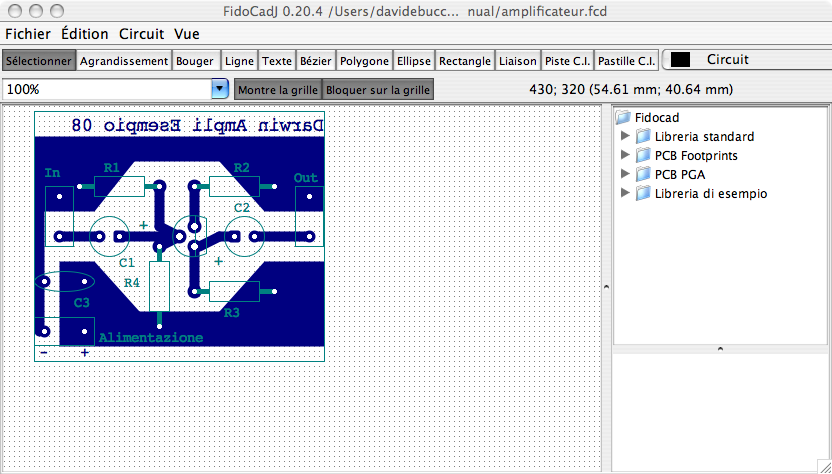
\includegraphics[width=1\textwidth]{amplificateur_complet} 

\caption{The job completed with the silk-screen.}


\label{fig_amplificateur_complet} 
\end{figure}


Once the drawing is completed, we will probably need to print\index{printing}
it either on a transparency to use it with a printing box\index{printing box}
or to use it with other methods such as the ``Press\&Peel''\index{Press&Peel@Press\&Peel}.
To do so we need to make invisible all the layers that we do not want
to print. This is done from the dialog window accessed from the menu
{}``Vista/Layer''. In our case it will be sufficient to hide the
layer 3 containing the silk-screen. The program will show the copper
layer only.

We will then print everything that is shown on the screen (obviously
NOT adapted to the size of the page, as we want to have the dimensions
set in the drawing), taking care of selecting the black and white
printing to ensure the maximum contrast. It may be useful to mirror
the whole drawing, depending on the technique chosen for the production
of the PCB\index{PCB}. Since our PCB is quite small, in its real
dimensions it will occupy only a small corner of the sheet (assuming
a standard ISO-UNI A4\index{A4}), as we can see in Figure~\ref{fig_amplificateur_impression}.

%
\begin{figure}
\centering \fbox{ 
\includegraphics[width=0.6\textwidth]{amplificateur_impression}} 

\caption{The PCB, as it appears when printed (mirrored) on a ISO-UNI A4 sheet.}


\label{fig_amplificateur_impression} 
\end{figure}


For information, below is the code generated for the PCB of the example
above (be careful with long lines!):
\begin{lstlisting}
[FIDOCAD]
TY 320 10 18 11 0 4 1 * Darwin Ampli Esempio 08 
TY 85 240 12 8 0 5 1 * + 
TY 44 239 12 8 0 5 1 * - 
PL 35 90 35 225 10 1
PL 55 130 95 130 10 1
PL 250 130 305 130 10 1
PL 215 130 230 130 10 1
PL 195 140 215 130 10 1
PL 115 130 175 130 10 1
MC 155 220 3 0 PCB.R01
MC 75 80 0 0 PCB.R01
MC 270 185 2 0 PCB.R01
MC 270 80 2 0 PCB.R01
MC 230 130 3 0 PCB.CE00
MC 115 130 1 0 PCB.CE00
MC 40 175 0 0 PCB.CC50
PL 190 80 190 120 10 1
PL 190 140 190 185 10 1
PL 155 80 155 120 10 1
PL 155 120 175 130 10 1
PL 155 140 175 130 10 1
PP 30 30 30 105 90 105 130 55 215 55 260 105 320 105 320 30 1
PP 320 240 320 155 260 155 215 205 135 205 90 155 55 155 55 240 1
MC 190 120 0 0 PCB.TO92
MC 305 90 1 0 PCB.CPBX352
MC 55 90 1 0 PCB.CPBX352
MC 80 225 2 0 PCB.CPBX352
TY 290 65 12 8 0 0 3 * Out 
TY 40 60 12 8 0 0 3 * In 
TY 95 225 12 8 0 0 3 * Alimentazione 
TY 70 190 12 8 0 0 3 * C3 
TY 230 95 12 8 0 0 3 * C2 
TY 115 150 12 8 0 0 3 * C1 
TY 120 170 12 8 0 0 3 * R4 
TY 220 200 12 8 0 0 3 * R3 
TY 230 55 12 8 0 0 3 * R2 
TY 100 55 12 8 0 0 3 * R1 
RV 30 5 320 255 3
\end{lstlisting} 

\section{Using the ruler}\index{ruler}
When drawing a PCB, it is often useful to measure distances in the working area. For example, you can check a track width, the clearance between two tracks or the total size of a card. FidoCadJ offers (since version 0.23.2) a ruler feature which allows you to easily perform those tasks. Just right click and drag. You should obtain a green ruler, like the one shown in figure~\ref{fig_fidocadj_righello}. If the right click and drag action is not used in your operating system, you can alternatively left click and drag while pressing the \keyevidence{Shift} key.
\begin{figure}
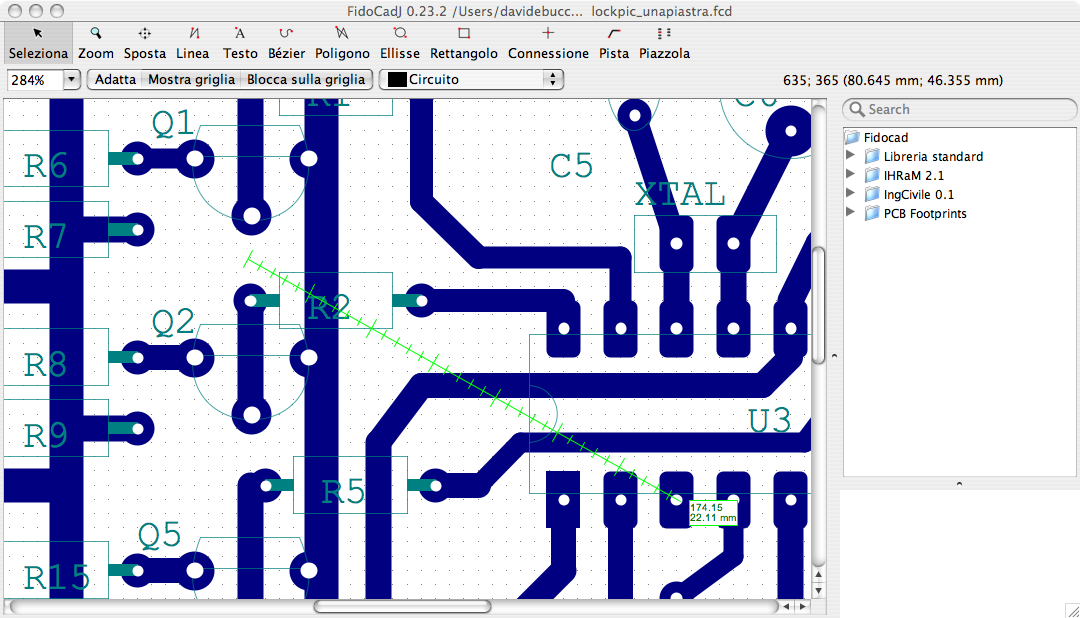
\includegraphics[width=\textwidth]{fidocadj_righello}
\caption{Right click and drag to activate the FidoCadJ ruler.}
\label{fig_fidocadj_righello}
\end{figure}
The total length measured is shown in FidoCadJ logical units\index{logical unit} as well as in millimeter. This is useful when the drawing is printed in the 1:1 mode (such as for PCB's).

\section{Arrow and stroke styles}
FidoCadJ allows to draw arrow heads\index{arrows} at the beginning and at the end of lines, B�zier curves and natural cubic splines. It also allows to specify whether the arrow should be at the beginning or at the end of an element (or both), and offers you a few different arrow styles. Arrow length can be negative: in this case, the arrow will extend outside the line or curve. Try and you will see the result.

A few stroke styles\index{stroke styles} are also available, for technical or mechanical drawings. Figure~\ref{fig_gyrator} shows an example in which an electrical circuit (a GIC\index{GIG}) is enclosed in a dashed rectangle. An arrow at the end of a B�zier curve is also being used. By doing double-click on this element, FidoCadJ shows a parameter window which should be similar to the one shown in figure~\ref{fig_parametri_bezier}. You can notice that the option box ``Arrow at start'' has been checked. FidoCadJ will thus trace an arrowhead by taking care of his orientation.
There are several different drawing styles for the arrow\index{arrow styles} as well for dashing \index{dashing styles}. You may try to play a little bit with them to appreciate their differences. If the arrow length is negative, the arrow will extend outside the length of the element, pointing towards it.

\begin{figure}
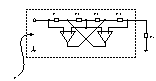
\includegraphics[width=\textwidth]{gyrator}
\caption{An electrical drawing (an Antoniou's GIC) in which some FidoCadJ extensions have been used.}
\label{fig_gyrator}
\end{figure}
\begin{figure}
\centering
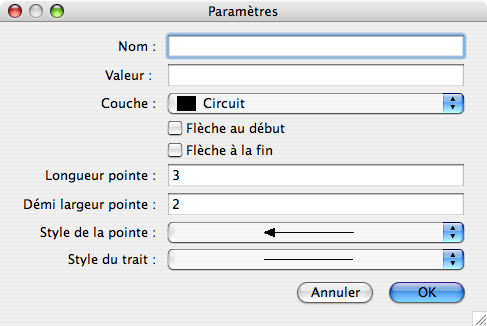
\includegraphics[width=.7\textwidth]{parametri_bezier}
\caption{The parameter window of the B�zier curve shown used in the schematics of figure~\ref{fig_gyrator} (French locale).}
\label{fig_parametri_bezier}
\end{figure}
The possibility of choosing a dashing style and putting arrowheads was not comprised in the original FidoCAD format. This unfortunately means that FidoCadJ drawings using those functionalities are not completely backward compatible with FidoCAD\index{FidoCAD} per Windows.
When you do chose to use a FidoCadJ extension, you need to know what you are doing. If you need to have a complete FidoCAD compatibility, you can activate the option ``Strict FidoCAD compatibility'' in the ``FidoCadJ extensions'' tab of the ``FidoCadJ preferences'' window. In this way, the program will not allow you to introduce graphical elements which would give compatibility problems with FidoCAD. If you need more details about the compatibility of the new graphical elements with FidoCAD\index{FidoCAD}, have a look at section~\ref{FCJ_extension}.


\section{Exporting}

One of the most important thing to me about FidoCadJ is the possibility
to create simple schematics for typographic use. For this reason I
introduced a feature that allows the exportation\index{exportation}
of drawings through a number of different file formats. 

To export the current drawing, select the command {}``Export'' from
the menu {}``File''. The Table~\ref{tab_esportazione} shows a
list of graphic file formats currently available. \marginpar{A vector
format\index{vector format} stores the elements that compose
the drawing. A bitmap format\index{bitmap format} works on a matrix
of pixels.} For every file format, the Table (but also the export dialog
in FidoCadJ) specifies whether it is vector or bitmap.
\footnote{The code structure of FidoCadJ allows the addition of other file format
quite easily. Please contact me if you like to participate to the
project.
}

For the bitmap file formats it may be useful to enable the option
{}``Anti aliasing'', to reduce the annoying effect of the quantization,
visible especially on diagonal lines. The resolution and the {}``Anti
aliasing'' options are not used when exporting to a vector file
format. In this case, you may instead specify a scaling factor.

The option {}``Black\&White'' allows the printing of any visible
layer in solid black. This is important for the preparation of films
to be used for typographic purposes or with a printing box.
\begin{table}
\centering \begin{tabular}{lp{0.7\textwidth}}
\toprule Format  & Comment\tabularnewline
\midrule \textsc{jpg}\index{JPG}  & Very widespread bitmap format. Since the compression used is lossy\index{lossy compression},
it is not suitable to for exporting FidoCadJ schematics. It is made
available due to its diffusion. \tabularnewline
\textsc{png}\index{PNG}  & Compressed bitmap format, suitable for exporting schematics. This
is probably the best way to export a FidoCadJ drawing when a vector
format cannot be used. \tabularnewline
\textsc{svg}\index{SVG}  & W3C standard vector format. Some internet browsers (such as the
recent versions of Safari\index{Safari}) allow its visualization
within a web page. Very good format for graphics and schematics, it
enables the use in applications such as Inkscape\index{Inkscape}
to modify the drawings made with FidoCadJ. There are currently some
limitations with the exportation of rotated and mirrored text. \tabularnewline
\textsc{eps}\index{EPS}  & Encapsulated Postscript vector format\index{Postscript}. Very
useful to those who use professional graphics applications, or want
to use a FidoCadJ drawing in a \LaTeX{}\index{\LaTeX{}@\LaTeX} document.
The drawings exportation should be fully working. This is the option
used to obtain Figure~\ref{fig_amplificateur}, page~\pageref{fig_amplificateur}
in this manual (passing through a \textsc{pdf} conversion, since I
use \textsc{pdf}\LaTeX{}\index{pdf\LaTeX{}@\textsc{pdf}\LaTeX}). \tabularnewline
\textsc{pgf}\index{PGF}  & Vector format to be used directly in a \LaTeX{}\index{\LaTeX{}@\LaTeX}
document, when using the \textsl{pgf} package, available in the CTAN
archive. This exportation option was thought in particular to export
schematics and uses an easily editable script. The text attributes
will not be translated. This allows the introduction of \LaTeX{}\index{\LaTeX{}@\LaTeX}
code directly into the drawing and it is the technique used in this
manual to obtain Figure~\ref{fig_schema}, page~\pageref{fig_schema}. \tabularnewline
\textsc{scr}\index{SCR}  & FidoCadJ allows the exportation of a drawing
to a script that can be imported in CadSoft\index{CadSoft} Eagle\index{Eagle}.
To use this feature, it is necessary to install the library \lstinline!FidoCadJLIB.lbr!
into the directory \lstinline!lbr! of the current installation of
Eagle. The library can be downloaded from FidoCadJ's website. At the
time of writing, this option works only with schematics containing
only the most common symbols. Some drawing elements such as pads and
tracks are not available yet. These will not be exported to the Eagle
script.\tabularnewline
\bottomrule  & \tabularnewline
\end{tabular}

\caption{List of all the export file formats available in FidoCadJ.}


\label{tab_esportazione} 
\end{table}



\section{Command line options}

The application is distributed as a file \lstinline!.jar!\index{jar},
which is a Java archive.%
\footnote{Except for the Macintosh\index{Macintosh} version, which is a stand
alone application.%
} In many operating systems, to run the application it should be enough
to double-click on the file, provided that a recent version of Java\index{Java}
is installed on the machine. Using Sun's\index{Sun} terminology,
the so called JRE\index{JRE}, or the Java Runtime Environment, is
all that is needed to run a program written in Java (but not to write
it: in that case the SDK would be necessary\dots). The minimum Java
version needed to run FidoCadJ is the 1.7, which has been around for
a few years now.

In some cases, it may be useful to run FidoCadJ from a command line
(the terminal\index{terminal} in the Unix\index{Unix} systems, or
the MS-DOS\index{MS-DOS prompt} Prompt in Windows\index{Windows}).
To do so, it is sufficient to run the command \lstinline!java!, with
the option \lstinline!-jar!: 
\begin{lstlisting} 
java -jar fidocadj.jar
\end{lstlisting}

If a file is specified in the command line\index{command line}, FidoCadJ
will try to open it. For example (on a Unix\index{Unix} machine):
\begin{lstlisting} 
java -jar fidocadj.jar ~/FidoCadJ/test.fcd 
\end{lstlisting}

FidoCadJ will be run and it will try to open the file \lstinline!~/FidoCadJ/test.fcd!
(provided that this exists).

There are some other interesting things FidoCadJ can do.
Option \lstinline!-h! shows a listing of the FidoCadJ options:
\lstset{language={},basicstyle=\scriptsize\ttfamily}
         
\begin{lstlisting}
[davidebucci@davide-bucci-portable]$ java -jar fidocadj.jar -h

This is FidoCadJ, version 0.24.6.
By Davide Bucci, 2007-2014.

Use: java -jar fidocadj.jar [-options] [file] 
where options include:

 -n     Do not start the graphical user interface (headless mode)

 -d     Set the extern library directory
        Usage: -d dir
        where 'dir' is the path of the directory you want to use.

 -c     Convert the given file to a graphical format.
        Usage: -c sx sy eps|pdf|svg|png|jpg|fcd|sch outfile
        If you use this command line option, you *must* specify a FidoCadJ
        file to convert.
        An alternative is to specify the resolution in pixels per logical unit
        by preceding it by the letter 'r' (without spaces), instead of giving
        sx and sy.
        NOTE: the coherence of the file extension is checked, unless the -f
        option is specified.

 -s     Print the size of the specified file in logical units.

 -h     Print this help and exit.

 -t     Print the time used by FidoCadJ for the specified operation.

 -p     Do not activate some platform-dependent optimizations. You might try
        this option if FidoCadJ hangs or is painfully slow.

 -l     Force FidoCadJ to use a certain locale (the code might follow
        immediately or be separated by an optional space).

 -k     Show the current locale.

 -f     Force FidoCadJ to skip some tests about sanity of the inputs.

 [file] The optional (except if you use the -d or -s options) FidoCadJ file to
        load at startup time.

Example: load and convert a FidoCadJ drawing to a 800x600 pixel png file
        without using the GUI.
  java -jar fidocadj.jar -n -c 800 600 png out1.png test1.fcd

Example: load and convert a FidoCadJ drawing to a png file without using the
        graphic user interface (the so called headless mode).
        Each FidoCadJ logical unit will be converted in 2 pixels on the image.
  java -jar fidocadj.jar -n -c r2 png out2.png test2.fcd

Example: load FidoCadJ forcing the locale to simplified chinese (zh).
  java -jar fidocadj.jar -l zh


[davidebucci@davide-bucci-portable]$ 
\end{lstlisting}
\lstset{language=FIDOCAD,
    basicstyle=\small\ttfamily}
    
The most simple option is \lstinline!-n!, with which the software\dots\ does nothing, i.e. it does not activate the GUI and just exits. In this case, the Java environment variable \lstinline!java.awt.headless! is set to true.
Obviously, this option is not so much useful alone, but it will be precious when using in combination with other functionalities we are about to describe.
Option \lstinline!-d! allows to specify the directory where FidoCadJ will seek for libraries to be loaded at startup. Option \lstinline!-c! allows to make FidoCadJ convert a FidoCAD file (which must be specified) into an image in a vector or raster format. This can be very useful, as FidoCadJ can be used as a converter in a non interactive way (along with the \lstinline!-n! option)

We can thus have a look at the first example given in the help:
        
\begin{lstlisting}
java -jar fidocadj.jar -n -c 800 600 png out1.png test1.fcd
\end{lstlisting}

FidoCadJ will run without activating the GUI and will export in the png\index{PNG} format the file \lstinline!test1.fcd!. The output file will be called \lstinline!out1.png! and will have a 800x600 pixel size.
There is an alternative version of the  \lstinline!-c! option, which will allow to specify how many pixels should be used to convert one logical unit (we will call this factor $r_\mathrm{p}$). FidoCadJ does not deal with half logical units (they are always integers), by choosing, let's say, $r_\mathrm{p}$ equal to two pixels per logical unit ensures that schematics will be always understandable (even if probably a little bit small). The $r_\mathrm{p}$ factor can be non integer, as in the following example:

\begin{lstlisting}
java -jar fidocadj.jar -n -c r1.25 png out2.png test2.fcd
\end{lstlisting}

To know the total size (in logical units) of a schematic, you can use the \lstinline!-s! option. Remember anyway that, during the exports, FidoCadJ adds always a $t_\mathrm{margin}=3$ logical units margin for each side of the drawing. So, if $t_\mathrm{w}$ is the width of the drawing in logical units given by \lstinline!-s!, you might expect that $p_\mathrm{w}$ the width of your drawing in pixel is calculated as follows:

\begin{equation}
p_\mathrm{w} = r_\mathrm{p} (t_\mathrm{w}+ 2 t_\mathrm{margin})
\end{equation}

Another interesting option, although a feature due to Java\index{Java}
more than FidoCadJ, is the possibility to modify the look of the application
(in the jargon of Java called look \& feel\index{look  feel@look \& feel}).
You can choose the look\&feel that you like without modifying a single
line of code. Here is something that Linux\index{Linux} users appreciate,
the GTK+\index{GTK+} look: 
\begin{lstlisting} 
java -Dswing.defaultlaf=com.sun.java.swing.plaf.gtk.GTKLookAndFeel -jar fidocadj.jar 
\end{lstlisting} 
There is also the classic Motif\index{Motif}
look \& feel, shown in Figure~\ref{fig_fidocadj_motif}\footnote{This style may somehow shock those well acquainted with very refined graphical interfaces such as Aqua, with MacOSX. However, I saw a few years ago a synchrotron control system which had a graphical interface based on Motif. Pretty though stuff!}: 
\begin{lstlisting}
java -Dswing.defaultlaf=com.sun.java.swing.plaf.motif.MotifLookAndFeel -jar fidocadj.jar 
\end{lstlisting} %
\begin{figure}
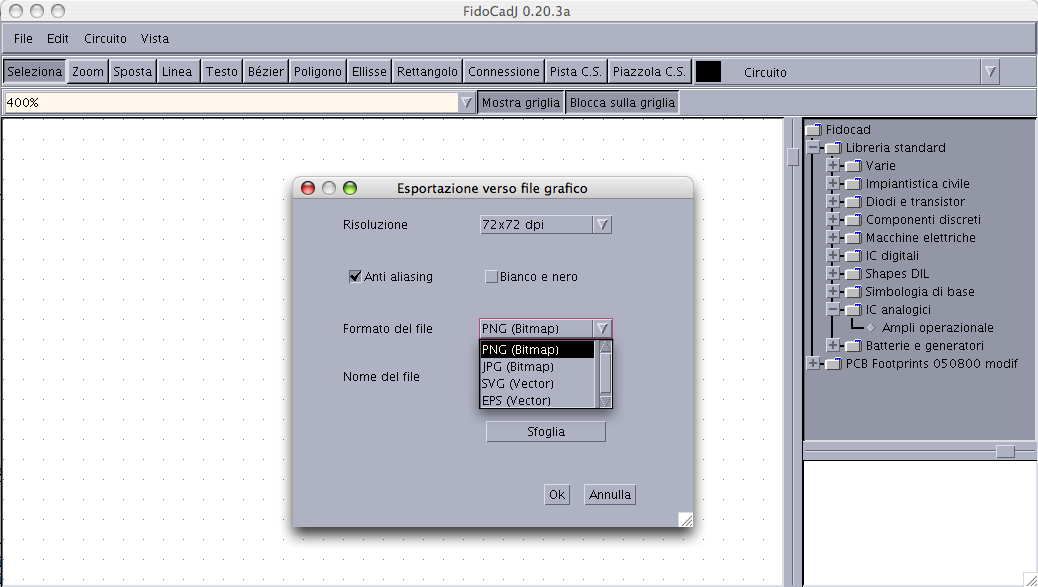
\includegraphics[width=1\textwidth]{fidocadj_motif} 

\caption{The appearance of the program on MacOSX\index{MacOSX}, using the Motif look \& feel.}

\label{fig_fidocadj_motif} 
\end{figure}


Obviously, the commands listed above are meant to be sent from a terminal,
making sure that the current directory contains the file \lstinline!fidocad.jar!
and writing everything on the same line.

\lstset{language=FIDOCAD,
 basicstyle=\small\ttfamily}

\section{Library management}
\subsection{Using library files}
A library is a collection of symbols which the user can include in his drawings. There is a collection of libraries included in the FidoCadJ packet, as well as the possibility of defining new symbols and libraries.
In fact, FidoCadJ allows us to specify a directory in which all the user library\index{library} files are placed (with the file extension \lstinline!.fcl!). This can be done through the menu {}``File/Options''. 

In some very special cases (or for testing), the libraries included in the FidoCadJ packet can be replaced by external ones.
If a file named \lstinline!FCDstdlib.fcl!
is present, its content will supersede the standard library\index{library!standard library} directly available in the application. Analogously, if a file named
\lstinline!PCB.fcl! is present, its content will replace the PCB
library\footnote{Pay attention to the use of capital letters, in particular if your operating system distinguish uppercase and lowercase letters in the
files management.}.

In version 0.23, thanks to Roby IZ1CYN, I could include the IHRaM 3.1 library\index{IHRaM library} directly inside the FidoCadJ distribution. I have done this because among all the libraries I have seen, this one has appeared to be one of the most complete and rationally constructed.
Exactly as it happens for the other libraries embedded in FidoCadJ, if there is a file called \lstinline!IHRAM.FCL! in the current library search path, this one will be loaded at the place of the version embedded in the program. You also have an electrical symbols library whose file is called \lstinline!elettrotecnica.fcl!.


Other files with \lstinline!.fcl! extension in the library search path will be considered as libraries and FidoCadJ will try to load them when it is starting. This is done when the application starts, when the user change the library search path, or when the ``Update libraries'' option in the ``Circuit menu'' is chosen.

FidoCadJ allows to split non standard macros (as the original FidoCAD\index{FidoCAD} does). This can be very useful when posting a drawing in a newsgroup, since in this way each macro not belong to the standard FidoCAD\index{FidoCAD} libraries is expanded into its graphic primitives. Who reads your post, thus, does not need to have the very same libraries you have installed in your system.
For copy/pasting, a command and a shortcut are available in the ``Edit'' menu, called ``Copy, split non standard macros'' (or \keyevidence{Control}+\keyevidence{M}\footnote{On MacOSX systems, the shortcut is \keyevidence{Command}+\keyevidence{M}}), in order to make sort that the copied drawing will have all the non standard macros split.
You might also save a file with the non standard macros split, by choosing `Save as..., split non standard macros''from the ``File'' menu. A dialog will appear to let you choose a new file name, since usually you do not want to overwrite the one you are working with.

\subsection{Defining new symbols}
FidoCadJ allows to create new libraries and new symbols. The adopted technique has been chosen in order to be as intuitive as possible. Here are the steps to follow:
\begin{itemize}
\item Make sure that a directory containing the user libraries has already been defined. If not, define it in the FidoCadJ user settings.
\item Draw what you want to convert into a new symbol.
\item Select what you just drawn and right click on it. A popup menu will appear, such as in figure~\ref{fig_symbol_o_matic}. 
\begin{figure}
  \begin{center}
    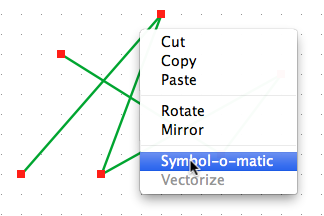
\includegraphics[width=.5\textwidth]{symbol_o_matic} 
  \end{center}
  \caption{The pop-up menu appearing with a right click allows to transform drawing elements into a symbol}
  \label{fig_symbol_o_matic} 
\end{figure}
\item Choose ``Symbol-o-matic'' and a dialog for the definition of the details of the newly created symbol will appear (see figure~\ref{fig_new_symbols}).
\begin{figure}
  \begin{center}
    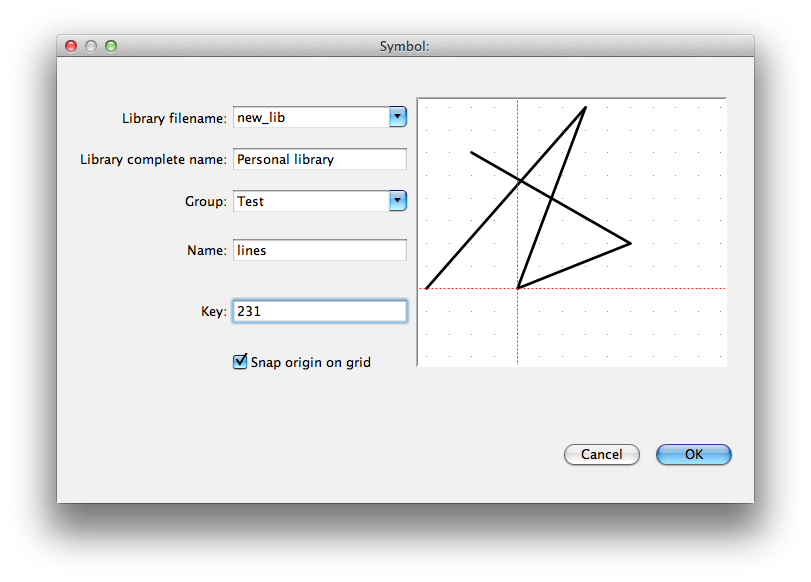
\includegraphics[width=.7\textwidth]{new_symbols} 
  \end{center}
  \caption{The new symbol definition dialog. Here you can set up all the important characteristics of the symbol. Note the origin defined by the two red axis.}
  \label{fig_new_symbols} 
\end{figure}
\item In the first field ``Library filename''\index{Library filename} you find the file name of the library in which the new symbol must be included. If you type a new name there, FidoCadJ will create a new file.
\item The second field ``Library complete name''\index{Library complete name} is the complete name of the library, the one which is shown in the library tree. You might write what you want there, but it is better to choose a short and meaningful one.
\item The third field ``Group''\index{Group} allows you to choose in which group you want to put the new symbol, inside the library. Once again, if you type a new name, a new group will be created.
\item The fourth field ``Name''\index{Name} is the name of the symbol, what it is shown in the library tree. Once again, choose a short but meaningful symbol.
\item The fifth field ``Key''\index{Key} is a very short tag which will identify the symbol in the code. It should be unique inside each library and should not contain spaces as well as characters such as parenthesis, dots, and so on. FidoCadJ will propose a short numerical code for you, but you might use mnemonic tags as well.
\item By clicking in the field on the right, you must choose the origin\index{Origin} of the symbol, the point which will be used for placing the symbol inside the drawing. You might choose to snap on the grid the position you choose by clicking on ``Snap origin on grid''.
\item Once you click on ``OK'', you should find your newly created symbol in the user library in the library tree in the main FidoCadJ window.
\end{itemize}
\begin{figure}
  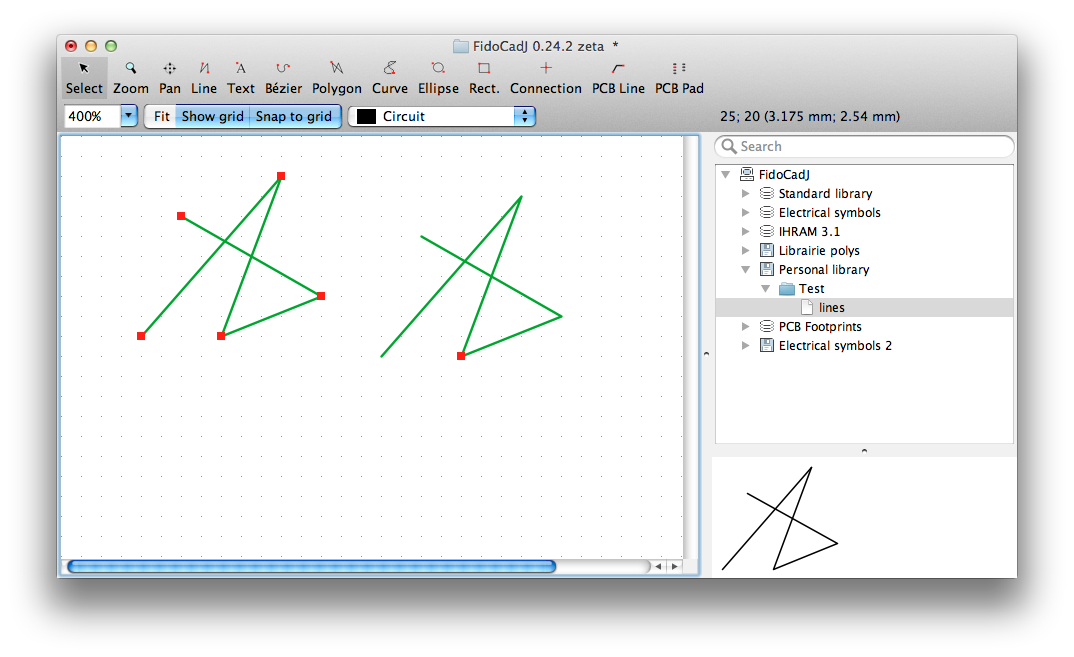
\includegraphics[width=1\textwidth]{new_symbol_use} 
  \caption{The freshly created symbol, shown in the symbol list and in the drawing. On the left, there is still the drawing which has been used for the symbol definition. Notice that just one control point is present for the new library symbol in the drawing.}
  \label{fig_new_symbol_use} 
\end{figure}
An example of an user symbol employed in a drawing is shown in figure~\ref{fig_new_symbol_use}. Note the difference between the selected part of the drawing on the left (actually what it has been used for defining a new symbol) and the new symbol placed on the right.
In fact, just one control point is available for the placement of the symbol and this control point corresponds to the choice of the origin while doing the symbol definition. It is thus useful to choose for that a point which has some relevance in your symbol.
You can split a symbol\index{Split a symbol} again in its primitives by selecting it and clicking on ``Vectorize''.

\subsection{Modifying existing symbols}
A few menu actions are available on symbols in the library tree. Once you select a symbol in an user library and do a right-click on it, a popup menu appears, as shown in figure~\ref{fig_popup_menu_lib}. Here you have several options:
\begin{figure}
  \begin{center}
    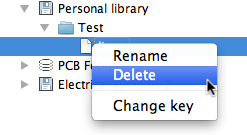
\includegraphics[width=.5\textwidth]{popup_menu_lib} 
  \end{center}
  \caption{The popup menu used for modifying symbol properties in an user library.}
  \label{fig_popup_menu_lib} 
\end{figure}
\begin{itemize}
\item ``Rename''\index{Rename (library symbol)} will change the displayed name of the symbol.
\item ``Delete''\index{Delete (library symbol)} will throw away the symbol. Be careful with this: if a drawing contains the symbol, it will be invalidated and disappear.
\item ``Change key''\index{Change key} is useful to modify the key associated to the symbol. Once again, this is something which must be done when the symbol has not been used in the drawing.
\end{itemize}
By using drag and drop\index{Drag and drop}, you might change the library or the category on which a symbol is categorized. Take into account that a symbol complete identification tag is composed by the library name, followed by the key of the symbol. Thus, moving a symbol from one library to another will invalidate drawings containing it.

All library operations are undoable, exactly as drawing operations. Bear in mind that empty libraries or groups are not shown.

\chapter{Drawing format, macros and FidoCAD libraries} \label{chap_formato}

This chapter contains a detailed description of the format used by
FidoCAD and, as a consequence, by FidoCadJ to store a drawing. It
is a simple text format which has the advantage of being very compact
and efficient. Since the format has never been described in detail
in a document, I will try to summarize all that I learnt about it.
Since I added a few extensions which are only available on FidoCadJ, I will try to describe them here as well. Remember that since version 0.23.4, FidoCadJ uses only the UTF-8\index{UTF-8} encoding\index{encoding} on all platforms.

\section{Header description}

All the files containing a drawing in the FidoCAD \emph{\index{FidoCAD}}
format must start with the tag \emph{\lstinline!{[}FIDOCAD{]}!.}
A program can therefore recognize the presence of FidoCAD commands
by reading this tag. In this regard, FidoCadJ is more tolerant
than the original FidoCAD \emph{\index{FidoCAD}} and it recognizes
and correctly interprets a file that does not contain the standard
header\emph{\index{header}}. Even commands containing text can therefore
be interpreted correctly as long as the number of incorrect
lines does not exceed a value set internally in the program (approx.
100). This ensures that FidoCadJ does not waste time working for a
few minutes for example trying to open a very large binary file.


\section{Coordinates system}

FidoCadJ works on a very simple coordinates system\emph{\index{coordinates system}}.
In practice, it has at its disposal a very large area identified only
by whole and positive coordinates. The length of every unit in x and
in y is fixed at \emph{$127\micron$}, a value that allows us to obtain
a good resolution for even the smallest SMD package without being
too fine for everyday use. In typographical terms, the FidoCadJ resolution is 200 dots per inch.

The original FidoCAD\emph{\index{FidoCAD}} had two different modes
of operation: PCB\emph{\index{PCB}} and electrical
schematic\index{electrical schematic}. In FidoCadJ this difference
has been blurred and appears only at the moment of printing the drawing.
It would therefore be advisable to set the program to resize an electrical
schematic to make better use of the size of the page, otherwise the printed result will have the size of a postage stamp.

\section{Drawing elements}

\label{sec_primitive} FidoCadJ can manage 12 drawing elements as
follows
\begin{itemize}
\item Line\index{line}
\item Filled or empty rectangle\index{rectangle} 
\item Simple text (obsolete)
\item Advanced text\index{text}
\item Filled or empty polyline\index{polyline}
\item Filled or empty ellipse\index{ellipse} 
\item B�zier curve \index{B�zier} 
\item Natural cubic spline curve \index{spline}
\item Electrical junction\index{connection}
\item PCB pad\index{PCB pad}
\item PCB track\index{PCB track}
\item Macro\index{macro}
\end{itemize}
We will proceed by analyzing each of them. In general, every element\index{element}
is identified by a command and a number of parameters\index{parameters}
(usually integer numbers or text strings) placed on the same line
and separated by a space character.


\subsubsection{Line}

The line primitive\index{line}\marginpar{Mathematicians would probably
find the term ``segment''\index{segment} more appropriate.} is identified
by the command \lstinline!LI!\index{LI} and its definition requires
only the begin and end coordinates and the layer: 
\begin{lstlisting}
LI x1 y1 x2 y2 l 
\end{lstlisting} 
the points $(x_{1},y_{1})$ and
$(x_{2},y_{2})$ represent respectively the initial and final coordinates,
while $l$ is the layer, characterized by an integer number between 0
and 15.

\textbf{FidoCadJ extension}: starting from FidoCadJ version 0.23, \lstinline!LI!\index{LI} can be followed in the next line by an extension:
\begin{lstlisting} 
FCJ a b c d e nv
\end{lstlisting}
where $a$ is an integer which represent the presence or not of the arrow heads at the extremes of the segment (have a look at table~\ref{tab_frecce_estremita}), $b$ represents the arrow head style (as table~\ref{tab_frecce_stile}). Parameters $c$ and $d$ give respectively the total length and the half width of the arrow head, while $e$ is an integer which gives the dash style. If $nv$ is equal to 1, the \lstinline!FCJ! command should be followed by two \lstinline!TY! commands giving the name and the value associated to this element.

\begin{table}
\centering

\begin{tabular}{ccp{.7\textwidth}}
\toprule
$a$ & Arrow head \\
\midrule
0   & none \\
1   & at the start side\\
2   & at the end side\\
3   & both sides\\
\bottomrule
\end{tabular}
\caption{Meaning of the $a$ parameter for the presence of an arrow head at the sides of a line or B�zier primitive.}
\label{tab_frecce_estremita}
\end{table}

\begin{table}
\centering
\begin{tabular}{ccp{.7\textwidth}}
\toprule
$b$ & Arrow head style \\
\midrule
0   & filled standard arrow head \\
1   & filled standard arrow head with quota line \\
2   & empty arrow head\\
3   & empty arrow head with quota line\\
\bottomrule
\end{tabular}
\caption{Meaning of the $b$ parameter for the arrow head style.}
\label{tab_frecce_stile}
\end{table}

\subsubsection{Filled or empty rectangle}

A rectangle\index{rectangle} filled or empty is identified by the
commands \lstinline!RP!\index{RP} and \lstinline!RV!\index{RV}
respectively, followed by the coordinates of the two vertices on one
of the two diagonals, and the layer. 
\begin{lstlisting} 
RP x1 y1 x2 y2 l 
RV x1 y1 x2 y2 l 
\end{lstlisting} the points $(x_{1},y_{1})$
and $(x_{2},y_{2})$ represent the two vertices and $l$ is the layer,
characterized by a whole number between 0 and 15.

\textbf{FidoCadJ extension}: starting from FidoCadJ version 0.23,  \lstinline!RP!\index{RP} and \lstinline!RV!\index{RV} can be followed in the next line by an extension:
\begin{lstlisting} 
FCJ e nv
\end{lstlisting}
where $e$ is an integer giving the dashing style. If $nv$ is equal to 1, the \lstinline!FCJ! command should be followed by two \lstinline!TY! commands giving the name and the value associated to this element.


\subsubsection{Simple text (obsolete)}

The simple text \index{simple text} was the first primitive provided
with the early versions of FidoCAD\index{FidoCAD}. FidoCadJ recognizes
it and simply writes text with size 12, regardless the current zoom\index{zoom}.

Since this primitive was considered obsolete\index{obsolete} by Lorenzo
Lutti\index{Lorenzo Lutti}, the creator of FidoCAD\index{FidoCAD},
FidoCadJ does exactly the same and, although this is correctly interpreted,
it is not available on the toolbar. FidoCadJ will store this element
exactly as it was advanced text and it will use the command \lstinline!TY!\index{TY}
when saving the file.

The command is \lstinline!TE!\index{TE} and the format is as follows:
\begin{lstlisting} 
TE x1 y1 �text to be written 
\end{lstlisting}
the point $(x_{1},y_{1})$ is where the string {}``text to be written''
will be positioned. Notice that the layer information is missing.
FidoCadJ will treat this object as it was placed on layer zero (circuit\index{circuit}).


\subsubsection{Advanced Text}

The primitive advanced text\index{advanced text} offers much more
flexibility with respect to simple text\index{simple text} introduced
above.

It is identified by the command \lstinline!TY!\index{TY}, followed
by a number of parameters to determine the text orientation (rotated\index{text!rotated}
or mirrored\index{text!mirrored}), as well as dimensions along $x$
and $y$ and the font used. Due to the quantity of information to
provide, the resulting command string is quite complex: 
\begin{lstlisting}
TY x1 y1 sy sx a s l f �text to be written 
\end{lstlisting}
The point $(x_{1},y_{1})$ is where the string ``text to be written''
will be positioned. The value of $s_{y}$ and $s_{x}$ indicates the
horizontal and vertical dimensions of the text in logical units\index{logical unit}.
I chose to let FidoCadJ respect the vertical dimension starting from
the horizontal one, and that aspect ratio will be chanced only if
this is strictly necessary. The text rotation is managed by the term
$a$, expressed in sexagesimal degrees, while the value of $s$ determines
the text style\index{text!style}, following table~\ref{tab_stile_testo}.
The layer is given by the usual term $l$, and $f$ indicates the
font to be used, or it can be an asterisk\index{asterisk}, to indicate
the use of the standard Courier New font\index{Courier New} If the font
name contains spaces these must be replaced with ``++''\index{++}.

%


%
\begin{table}
\centering \begin{tabular}{llp{0.7\textwidth}}
\toprule Bit  & Weight  & Behavior \tabularnewline
\midrule 0  & 1  & text in bold\tabularnewline
2  & 4  & mirrored text\tabularnewline
\bottomrule  &  & \tabularnewline
\end{tabular}

\caption{Function of the bits in the text style term.}


\label{tab_stile_testo} 
\end{table}


The maximum length of the text\index{maximum length of text} is about
80 words. The counting is done in words and not in characters because
in the internal structure of the program the words (and command terms)
are separated when a line is being interpreted.


\subsubsection{Filled or Empty polyline}

A polyline\index{poliline} filled or empty is indicated with the
commands \lstinline!PP!\index{PP} and \lstinline!PV!\index{PV}
respectively, followed by the coordinates of the vertices that define
the polyline, and the layer. The commands are 
\begin{lstlisting}
PP x1 y1 x2 y2 ... l 
PV x1 y1 x2 y2 ... l 
\end{lstlisting} 
where the points $(x_{1},y_{1})$, $(x_{2},y_{2})$\dots\ are the vertices
that define the polyline and $l$ is the layer, characterized by a
whole number between 0 and 15. The length of the command line can
thus vary depending on the number of vertices used. The maximum number
of vertices\index{maximum number of vertices} available has been
arbitrarily fixed at 20.

\textbf{FidoCadJ extension}: starting from FidoCadJ version 0.23,  \lstinline!PP!\index{PP} and \lstinline!PV!\index{PV} can be followed in the next line by an extension:
\begin{lstlisting} 
FCJ e nv
\end{lstlisting}
where $e$ is an integer giving the dashing style. If $nv$ is equal to 1, the \lstinline!FCJ! command should be followed by two \lstinline!TY! commands giving the name and the value associated to this element.


\subsubsection{Filled or Empty ellipse}

An ellipse\index{ellipse} filled or empty is identified by the commands
\lstinline!EP!\index{EP} e \lstinline!EV!\index{EV} respectively,
followed by the coordinates of the two vertices on the diagonal and
the layer number. 
\begin{lstlisting} 
EP x1 y1 x2 y2 l 
EV x1 y1 x2 y2 l 
\end{lstlisting} 
the point $(x_{1},y_{1})$ represents the first
vertex on the diagonal, $(x_{2},y_{2})$ is the second vertex, and
$l$ is the layer, identified by a whole number between 0 and 15.


\textbf{FidoCadJ extension}: starting from FidoCadJ version 0.23,  \lstinline!EP!\index{EP} and \lstinline!EV!\index{EV} can be followed in the next line by an extension:
\begin{lstlisting} 
FCJ e nv
\end{lstlisting}
where $e$ is an integer giving the dashing style. If $nv$ is equal to 1, the \lstinline!FCJ! command should be followed by two \lstinline!TY! commands giving the name and the value associated to this element.


\subsubsection{B�zier curve}

A B�zier\index{B�zier} curve segment, in its cubic variant, is identified
by four vertices, which are thus required by its associated command
\lstinline!BE!\index{BE}: 
\begin{lstlisting} 
BE x1 y1 x2 y2 x3 y3 x4 y4 l 
\end{lstlisting} 
where $P_{1}\equiv(x_{1},y_{1})$, $P_{2}\equiv(x_{2},y_{2})$,
$P_{3}\equiv(x_{3},y_{3})$ e $P_{4}\equiv(x_{4},y_{4})$ are the
four control points of the B�zier\index{B�zier} curve segment, while
$l$ is the layer, identified by a whole number between 0 and 15.
Given the four points defined above, the curve segment is computed
through the expression \begin{equation}
B(t)=(1-t)^{3}P_{1}+3t(1-t)^{2}P_{2}+3t^{2}(1-t)P_{3}+t^{3}P_{4},\end{equation}
where $t\in[0,1]$ is a parameter.

\textbf{FidoCadJ extension}: starting from FidoCadJ version 0.23, \lstinline!BE!\index{BE} can be followed in the next line by an extension:
\begin{lstlisting} 
FCJ a b c d e nv
\end{lstlisting}
where $a$ is an integer which represent the presence or not of the arrow heads at the extremes of the curve (have a look at table~\ref{tab_frecce_estremita}), $b$ represents the arrow head style (as table~\ref{tab_frecce_stile}). Parameters $c$ and $d$ give respectively the total length and the half width of the arrow head, while $e$ is an integer which gives the dash style. If $nv$ is equal to 1, the \lstinline!FCJ! command should be followed by two \lstinline!TY! commands giving the name and the value associated to this element.

\subsubsection{Natural cubic spline (complex curve)}
A natural cubic spline\index{spline} is defined by a certain number of vertices. The curve crosses each vertex and it is calculated in such a way that it is very smooth.\footnote{ \href{http://www.cse.unsw.edu.au/~lambert/splines/natcubic.html}{http://www.cse.unsw.edu.au/\textasciitilde lambert/splines/natcubic.html}} In the FidoCadJ format, a spline is identified by commands \lstinline!CV!\index{CV} and \lstinline!CP!\index{CP}:
\begin{lstlisting}
CV aa x1 y1 x2 y2 ... l
CP aa x1 y1 x2 y2 ... l
\end{lstlisting}
the $aa$ parameter is equal to 1 if the curve is closed, or it is 0 otherwise. Vertices $(x_1, y_1)$, $(x_2, y_2)$\dots define the spline and $l$ is the layer, an integer ranging from 0 to 15.
The lenght of the command line can thus vary depending on how much vertices are considered.
As for polygons, the maximum number of vertices\index{maximum number of vertices} available is internally fixed to a little less of 5000. This primitive has been introduced in version 0.24 and is not present in the original FidoCAD\index{FidoCAD}.

\textbf{FidoCadJ extension}: \lstinline!CV!\index{CV} and \lstinline!CP!\index{CP} can be followed in the following line by an extension:
\begin{lstlisting} 
FCJ a b c d e nv
\end{lstlisting}
where $a$ is an integer which represent the presence or not of the arrow heads at the extremes of the curve (have a look at table~\ref{tab_frecce_estremita}), $b$ represents the arrow head style (as table~\ref{tab_frecce_stile}). Parameters $c$ and $d$ give respectively the total length and the half width of the arrow head, while $e$ is an integer which gives the dash style. If $nv$ is equal to 1, the \lstinline!FCJ! command should be followed by two \lstinline!TY! commands giving the name and the value associated to this element.

\subsubsection{Electrical junction}
The electrical junction\index{junction} primitive is simply a filled
circle of constant dimensions and it is used to represent a connection
in an electrical schematic. It is identified by the command \lstinline!SA!\index{SA}
and it only requires its coordinates and layer: 
\begin{lstlisting}
SA x1 y1 l 
\end{lstlisting} 
With FidoCadJ, the diameter of the circle
is fixed internally into the program to two logical units.

If \lstinline!SA!\index{SA} is followed by \lstinline!FCJ!, the \lstinline!FCJ! command should be followed by two \lstinline!TY! commands giving the name and the value associated to this element.

\subsubsection{PCB pad}

A PCB pad\index{PCB pad} is identified by the command \lstinline!PA!\index{PA}
and it is characterized by its style (round, rectangular, rectangular
with smoothed corners) and the diameter of its internal hole: 
\begin{lstlisting}
PA x1 y1 dx dy si st l 
\end{lstlisting} 
where the point $(x_{1},y_{1})$
represents the position of the pad, $d_{x}$ is the pad's width (along
the $x$ axis), $d_{y}$ is the height (along the $y$ axis). The
value $s_{i}$ is the diameter of the pad's hole, while $s_{t}$ is
the pad's style: 
\begin{itemize}
\item [0] oval pad
\item [1] rectangular pad
\item [2] rectangular pad with smoothed corners
\end{itemize}
The value of $l$ must be a whole number to indicate the layer where
the pad is to be placed.
If \lstinline!PA!\index{PA} is followed by \lstinline!FCJ!, the \lstinline!FCJ! command should be followed by two \lstinline!TY! commands giving the name and the value associated to this element.

\subsubsection{PCB track}

The PCB track\index{PCB track} is essentially a segment, the width
of which can be specified. The corners at the extremes of the segment
are always rounded to facilitate the connection with other PCB tracks
or pads. The command to be used is \lstinline!PL!\index{PL}, with
the following format: 
\begin{lstlisting} 
PL x1 y1 x2 y2 di l 
\end{lstlisting}
The track is drawn between the points $(x_{1},y_{1})$ and $(x_{2},y_{2})$,
with total width $d_{i}$, and the layer used is $l$. The width $d_{i}$ can be non integer.
If \lstinline!PL!\index{PL} is followed by \lstinline!FCJ!, the \lstinline!FCJ! command should be followed by two \lstinline!TY! commands giving the name and the value associated to this element.

\subsubsection{Macro call}

A macro\index{macro} is a drawing or a symbol contained in a library.
Generally, this is the way frequently used electrical symbols are
represented. The command used to calla macro is \lstinline!MC!\index{MC},
and the call is done as follows: 
\begin{lstlisting} 
MC x1 y1 o m n 
\end{lstlisting} 
The macro is drawn using position $(x_{1},y_{1})$
as the reference, and the orientation is defined by the value of $o$
(multiplied by 90\textdegree{} clockwise) and if $m$ is equal to 1 the macro
is mirrored. the last parameter, $n$, is the macro's name within
the library, specified as \emph{library.code}.

If \lstinline!MC!\index{MC} is followed by \lstinline!FCJ!, the \lstinline!FCJ! command should be followed by two \lstinline!TY! commands giving the name and the value associated to this element.

\section{FidoCadJ extensions}
\label{FCJ_extension}
Since version 0.21, FidoCadJ has started to introduce a few refinements over the original FidoCAD format\index{FidoCadJ extension}. The FidoCadJ extensions are represented in the code by the command \lstinline!FCJ!\index{FCJ}. This command is not used alone, but means that FidoCadJ needs to specify additional information on what it is specified in the previous line.
Here is an example:
\begin{lstlisting}
[FIDOCAD]
MC 40 30 0 0 080
FCJ
TY 50 35 4 3 0 0 0 * R1
TY 50 40 4 3 0 0 0 * 47k
\end{lstlisting}
The presence of the \lstinline!FCJ! command indicates that the name and the value of the macro speficed in the first line are given by the two \lstinline!TY! commands which follow. Only the coordinates and the fonts are taken into account for the text rendering.

FidoCadJ allows to activate a ``strict FidoCAD compatibility mode'', in which all extensions are disabled. This way, FidoCadJ will be perfectly compatible with the original FidoCAD\index{FidoCAD}, except that FidoCadJ will continue using the UTF-8\index{UTF-8} encoding\index{encoding} instead of the old CP-1252\index{CP-1252} used by FidoCAD\index{FidoCAD}.
FidoCAD for Windows is unable to understand the additional informations carried by the \lstinline!FCJ!\index{FCJ} command. When reading with the original FidoCAD a FidoCadJ drawing containing some extension, the program will prompt a few errors and will give a result which is different from the original FidoCadJ drawing.
The results will depend on what extension has been used: a dashed line will be rendered as continuos, the arrow heads will be not drawn. The text associated to the name and the value of a macro will instead be perfectly rendered.

Figure~\ref{fig_gyrator_n} shows what can be obtained using FidoCAD\index{FidoCAD} to read the FidoCadJ file which describes~\ref{fig_gyrator}. After ignoring the FidoCAD errors, there are some details missing (the dashing and the arrow), but the overall drawing is still understandable.

\begin{figure}
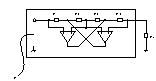
\includegraphics[width=\textwidth]{gyrator_n}
\caption{Figure~\ref{fig_gyrator} as it would appear on FidoCAD for Windows.}
\label{fig_gyrator_n}
\end{figure}

An important difference from the original FidoCAD\index{FidoCAD} is that FidoCadJ allows to save a certain number of configuration hints in the output files. The command which is used for that is \lstinline!FJC!\index{FJC} and it should normally be placed at the very beginning of the file. The next paragraphs will describe the cases which are treated.

 \subsection{Layer setup}
 The layer setup is specified with the command \lstinline!FJC L!\index{FJC L}. FidoCadJ saves data only if the corresponding layer has been modified from its default state. The syntax is as follows:
 \begin{lstlisting}
 FJC L n xxxx yy
\end{lstlisting}
where $n$ represents the layer number (ranging from 0 to 15), $xxxx$ is a 32 bit integer containing settings about the RGB color to be used. The red component is contained in bits 16-23, the green one in bits 8-15 and the blue one in bits 0-7.
The value $yy$ is a single precision floating point constant which gives the layer transparency, comprised between 0.0 (completely transparent) and 1.0 (completely opaque).

A second important information is the name of the layer, specified (if the user has changed it) as follows:
\begin{lstlisting} 
FJC N n aaaaa
\end{lstlisting}
where $n$ is the number of the layer (integer from 0 to 15), whereas {\normalfont \itshape aaaa} is the name of the layer to be considered. If this command is not present, the name of the layer will be the one used by default by FidoCadJ, depending on the language and on the local configuration of the operating system.

\subsection{Electrical connection setup}
The size of the black circle used to indicate an electrical connection can be modified by the user.
When the FidoCadJ extensions are active, the selected value is saved in the file with the \lstinline!FJC C!\index{FJC C} command as follows:
\begin{lstlisting}
FJC C aaaa
\end{lstlisting}
where $aaaa$ is a double precision floating point value (positive) which gives the diameter of the electrical connection, in FidoCadJ logical units.

 \subsection{Stroke width}
 The stroke width for the ``pen'' used during the drawing of electrical schematics can be modified. FidoCadJ adopts the command \lstinline!FJC A!\index{FJC A} to specify the stroke width of the lines, ovals, B�zier, splines, rectangles and polygons. The width can be a double precision constant.
\begin{lstlisting}
FJC A aaaa
\end{lstlisting}
Where $aaaa$ represents the stroke width (in logical units). The default width is internally defined to 0.5 logical units. In older versions of FidoCadJ, a command \lstinline!FJC B bbbb!\index{FJC B} was used to specify the stroke width of curved lines (ovals, B�zier). Since version 0.23.6, this differentiation has been eliminated and this command is no longer adopted.

\section{Syntax errors tolerance}

FidoCadJ is designed to tolerate errors\index{error tolerance} or
or certain syntax errors in the commands passed to the program. Obviously,
unless you have a crystal ball connected as a USB device\index{crystal ball},
the program will not be able to correct errors but it will simply
skip (and delete) all the lines involved.

An exception to this behavior is that a number of elements can
be specified without the layer, which will be considered part of the
layer\index{layer} 0 (schematics). This is for backward compatibility
with FidoCAD\index{FidoCAD}.


\section{Libraries format}

The file structure of a library file is quite simple:

\begin{lstlisting} 
[FIDOLIB Librairie de base]
{Syboles de base}
[000 Terminal]
LI 100 100 102 100
EV 102 98 106 102
[010 Terminal +]
LI 100 100 102 100
EV 102 98 106 102
LI 103 100 105 100
LI 104 99 104 101
[020 Terminal -]
LI 100 100 102 100
EV 102 98 106 102
LI 103 100 105 100
...
\end{lstlisting} 
The first
line contains, between square brackets\index{square brackets}, the
library's name (preceded by FIDOLIB\index{FIDOLIB}). The second line
must contain, between curly brackets, the library category under which
the macros, specified later on in the file, will be stored.

Each macro is composed by a header\index{header} (between square
brackets) and a sequence of commands. The header is constituted by
a \emph{part name} (which must be unique within the library) and its
description. The part name will be used within a FidoCadJ script, while
the description helps the user while browsing all the macros\index{macro}
contained in the file. The commands are nothing else than FidoCadJ
drawings, where the coordinate point (100,100) is used as the origin.
This is the point that will be used as the reference when the macro
will be called. In a FidoCadJ script a macro is identified by {}``library.macro''
used with the MC\index{MC} command.

Nothing prevents the calling of a macro within another macro. However,
recursion\index{recursion} (i.e. a macro that calls itself) must
be avoided.

A library \textit{must not contain} among the macro definitions any information about the FidoCadJ configuration. In other words, commands \lstinline!FJC!\index{FJC} should \textit{never} appear inside a library file.

\section{Standard Libraries}

FidoCadJ already contains two libraries traditionally supplied with
FidoCAD\index{FidoCAD}. In particular these are the standard library\index{standard library}
and the library that contains the PCB symbols\index{PCB library}. Another library which has been developed for FidoCAD\index{FidoCAD} and which has been proved so useful that it has been included as part of FidoCadJ is the IHRAM one. IHRAM stands for \lstinline!it.hobby.radioamatori.moderato! and it is an italian Usenet discussion group. 

However, it is possible to override the content of these internal
libraries by specifying ({}``File/Options/Libraries Directory'' menu)
a directory containing the libraries to be loaded. If a file named
\lstinline!FCDstdlib.fcl! is present in this directory, its content
will be used instead of the standard library. If a file named
\lstinline!PCB.fcl! is present, its content will be used instead the internal PCB library. Other libraries having different file
names (but still with extension \lstinline!fcl!) will be loaded together
with the standard libraries. If there is a file called \lstinline!IHRAM.FCL! in the current library search path, this one will be loaded at the place
of the version embedded in the program. You also have an electrical symbols library whose file is called \lstinline!elettrotecnica.fcl!.

FidoCadJ considers the libraries above as part of the standard set. In other words, it will not split the symbols contained in drawings, if they belong to those libraries, except when the option ``Strict compatibility with FidoCAD''\index{Compatibility with FidoCAD} is active. In this case, only the original FidoCAD\index{FidoCAD} library is considered as standard, exactly how it used to do the original software.


\chapter{Conclusion} We have seen in this manual how to use FidoCadJ
to draw an electrical schematic or a simple PCB. At this stage the
reader should possess all the elements necessary to use FidoCadJ effectively
for his needs.

FidoCadJ should not be considered uniquely for the
electronics design. It can be used for any type of 2D drawing and
in many situations, provided that specific libraries are available.

The advantages of a free program is that it is completely open
to its user community. For this reason, your feedback is very
important (at least to understand if the project is worth to be developed
further, and in which direction). To contact me, open an issue on the GitHub FidoCadJ  project.\footnote{\href{https://github.com/DarwinNE/FidoCadJ/issues}{https://github.com/DarwinNE/FidoCadJ/issues}}

\appendix

\chapter{Platform-specific information} \label{specifics} 


\section{MacOSX}

One of the most frequent criticisms raised against the early versions
of FidoCadJ from Macintosh users (like me, by the way) was the poor
integration of the program on MacOSX. Starting since version 0.21.1,
FidoCadJ is making specific efforts to comply better with the look
and the philosophy of Mac's native applications. For this reason,
some details in the program are slightly different when FidoCadJ is
run on an Apple platform: 
\begin{itemize}
\item by default FidoCadJ uses the Quaqua%
\footnote{\href{http://www.randelshofer.ch/quaqua/}{http://www.randelshofer.ch/quaqua/}%
}\index{Quaqua} look and feel when the complete application (FidoCadJ.app\index{FidoCadJ.app}
instead of fidocadj.jar\index{fidocadj.jar}) is run. Since Quaqua
may slow down the performance on not so recent machines, it is possible
to disable it through the settings of the Preferences menu
\item The menu bar is shown at its place, that is the top of the screen
\item The menu items {}``Preferences'' and {}``About FidoCadJ'' are
at their place, which is under the FidoCadJ menu. 
\item The program tells the operating system that it can open \lstinline!.fcd!
files; These are associated to a specific icon, which should be sufficiently
evocative.
\end{itemize}

\subsection{How to download and execute FidoCadJ on MacOSX}
FidoCadJ can work with a MacOSX\index{MacOSX} version more recent than 10.6 (Snow Leopard\index{Snow Leopard}).
Under the hood, FidoCadJ needs at least the 1.7 version of Java. For marketing reasons, Apple does not seem to be prone to install Java with the last versions of MacOSX\index{MacOSX}. This is an essential piece of software needed for running FidoCadJ, so you might download and install it. By the way, Apple does not allow to distribute his App Store\index{App Store} software based on Java or distributed under GPL. This is one of the most important reasons for which it is quite improbable that FidoCadJ will be ported to iPad\index{iPad} and iPhone\index{iPhone}.

Even if you can use directly the Java archive \lstinline!fidocadj.jar! as you would do on other operating systems, on MacOSX you can use the specifically tailored application. Everything works just like a native application: you can download the disk image at the following link:

{\small
\href{https://github.com/DarwinNE/FidoCadJ/releases/download/v0.24.6/FidoCadJ_MacOSX.dmg}{https://github.com/DarwinNE/FidoCadJ/releases/download/v0.24.6/FidoCadJ\_MacOSX.dmg}}\\
You can then open the disk image and move \lstinline!FidoCadJ.app! in the \lstinline!Applications! folder, where you can use it exactly like any other Macintosh application. To uninstall FidoCadJ, just drag  \lstinline!FidoCadJ.app! in the trash bin.


\section{Linux}
\label{installazione_linux} \textsl{by Roby IZ1CYN}\\


Prerequisite: JRE\index{JRE} 6 from Sun\index{Sun} and/or OpenJDK\index{OpenJDK}
6 JRE\index{JRE} (o previous versions compatible with the program's
specifications) must be installed. In paragraph \ref{inst_testo}
the installation of the program using only commands from a terminal
will be described. In paragraph \ref{inst_grafica}, the interaction
with a graphical environment will be used instead. A poor configuration of your Java runtime environment will determine poor performances of FidoCadJ\footnote{N.d.c. I swear, it is true! \textit{Please}, do not insult me if your favorite Linux distribution comes with an higly unreliable version of Java.}.

\subsection{Using any platform, from terminal}

\label{inst_testo} Download the program using the \lstinline!wget! command:


%\lstset{language=plain,%
%   basicstyle=\tiny\ttfamily}
    
\begin{lstlisting}
$ wget https://github.com/DarwinNE/FidoCadJ/releases/download/v0.24.6/fidocadj.jar
--00:48:18--  https://github.com/DarwinNE/FidoCadJ/releases/download/v0.24.6/fidocadj.jar
           => `fidocadj.jar'
Resolution of github.com is being done... xxx.xxx.xxx.xxx
Connection to github.com is being done... xxx.xxx.xxx.xxx connected.
HTTP request sent, waiting for answer... 200 OK
Length: 343,207 (335K) [application/java-archive]

100%[====================================>] 343,207      422.48K/s             

00:48:30 (420.55 KB/s) - "fidocadj.jar" saved [343207/343207]
$
\end{lstlisting}
\lstset{
    basicstyle=\small\ttfamily}

Alternatively, or if you are experiencing problems, you can download the file from any browser from the following URL:

\href{https://github.com/DarwinNE/FidoCadJ/releases/download/v0.24.6/fidocadj.jar}{https://github.com/DarwinNE/FidoCadJ/releases/download/v0.24.6/fidocadj.jar}

and save the file in your \lstinline!/home/! directory.
    


Let's create a new directory (but at first we will become a superuser\index{superuser} by using \lstinline!su! or \lstinline!sudo -s!):

\begin{lstlisting}
$ su
-> enter password
# mkdir /usr/bin/fidocadj
\end{lstlisting}

\dots\ and we can move there the downloaded file (substitute \lstinline!<user>! with the user name of the account where the file has been downloaded):

\begin{lstlisting}
# mv /home/<user>/fidocadj.jar /usr/bin/fidocadj
\end{lstlisting}

Let's make the file an executable

\begin{lstlisting}
# chmod +x /usr/bin/fidocadj/fidocadj.jar
\end{lstlisting}

And we must not forget to come back to be normal users:

\begin{lstlisting}
# exit
\end{lstlisting}

And now, we can execute the program:

\begin{lstlisting}
$ /usr/bin/fidocadj/fidocadj.jar
\end{lstlisting}

\subsection{On a graphical system}
\label{inst_grafica}
In the example, it will be an Ubuntu\index{Ubuntu} 8.04, but things does not change so much for older or newer versions:

\begin{itemize}
\item {Let's download the file from the browser, or with Gwget or similar tools.}

\item�{We can then launch our File Manager (Nautilus, Konqueror\dots) as a root (if we do not have a specific command in the menu, we just need to launch it from the console by using \lstinline!sudo nautilus!). We can create the following directory:
\begin{lstlisting}
/usr/bin/fidocadj
\end{lstlisting}
and then move there the file we just downloaded. It will be somewhere in: 
\begin{lstlisting}
/home/<user>/
\end{lstlisting}}

\begin{figure}
\centering
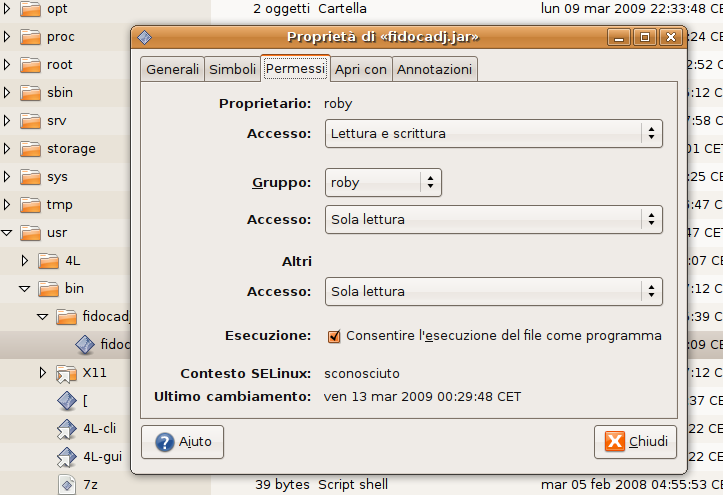
\includegraphics[width=.8\textwidth]{permessi}
\caption{The setting of file rights, on Ubuntu\index{Ubuntu} 8.04.}
\label{fig_permessi}
\end{figure}

\item {Let's do right click on the file, from the window we select the tab ``rights'', we add the check mark in front of the ``Allow the execution of the file as a program'', as shown in the figure~\ref{fig_permessi}}

\begin{figure}
\centering
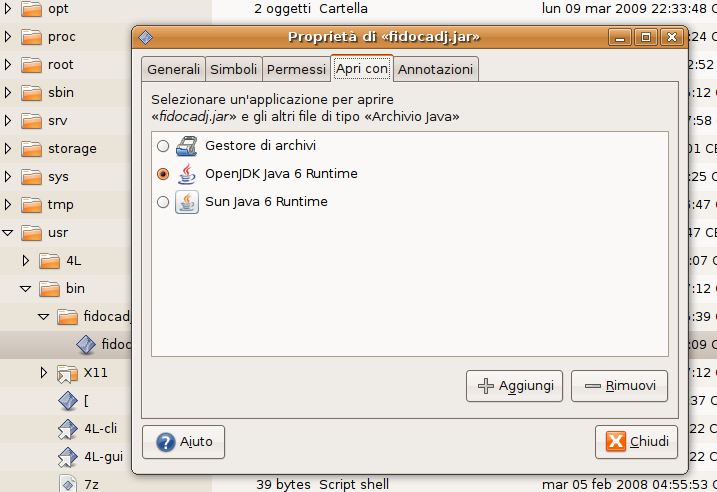
\includegraphics[width=.8\textwidth]{java6}
\caption{Set the execution with the Java virtual machine, on Ubuntu\index{Ubuntu} 8.04.}
\label{fig_java6}
\end{figure}

\item {We can select the tab ``Open as'' and select ``OpenJDK Java 6 Runtime'' or ``Sun Java 6 Runtime'', as it can be seen in figure~\ref{fig_java6}.}

\item {Let's click on ``Close'' and we are now ready to execute FidoCadJ: a double click on the executable, or we can add it to the main menu. The command to add is just \lstinline!/usr/bin/fidocadj/fidocadj.jar!.}
\end{itemize}


\section{Windows}
Since version 0.23, when FidoCadJ recognizes a Windows platform, it will try to use the native Look and Feel.

 \subsection{How to download and execute FidoCadJ}
Very often, if you have Java installed, you just have to download the  \lstinline!fidocadj.jar! file and run it with a double click. If after the download your operating system sees it as a \lstinline!zip! archive, probably Java is not available on your computer. Oracle allows to freely download and install an up to date version of the Java runtime:

\href{http://www.java.com/it/download/}{http://www.java.com/it/download/}

\section{Android}
A specific version of FidoCadJ for Android is available. It shares much of the source code with the PC version, but all the graphical user interface code had to be rewritten. It should work on a variety of devices with at least Android 4.0: smartphones as well as tablets. For example, figure~\ref{fig_fidocadj_s5} shows the appearance of FidoCadJ for Android with a Samsung S5 smartphone.

There are some minor differences between the Android application and the PC application described in the manual. They of course are perfectly compatible for the file format and can exchange drawings.
\begin{figure}
\centering
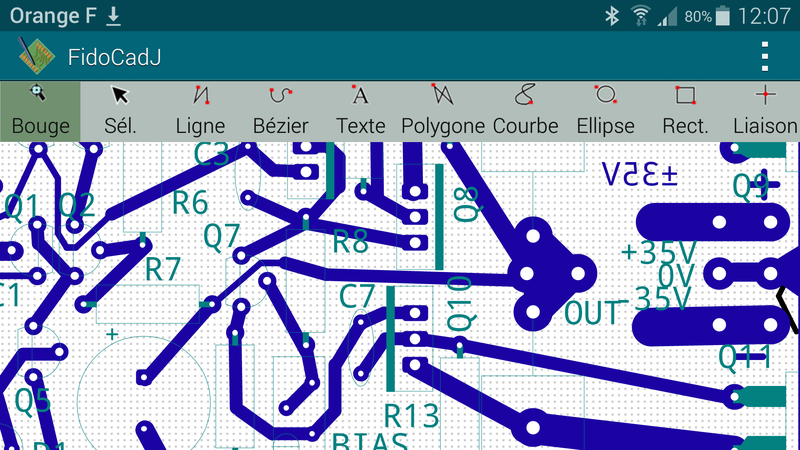
\includegraphics[width=.8\textwidth]{fidocadj_s5}
\caption{FidoCadJ for Android, running on a Samsung S5 smartphone.}
\label{fig_fidocadj_s5}
\end{figure}

\begin{itemize}
\item You can not create and edit user libraries, but you can use those built on a PC.
\item You store the user libraries in the external filesystem (the ``SD card''), in the \lstinline!FidoCadJ/Libs! directory.
\item The symbols are not shown all the time to save space: you have to sweep your finger on the right of the screen to show them.
\item You have an additional button in the toolbar, which allows you to move and zoom the shown portion of the drawing. While in this ``Move'' state, touch the screen and move your finger to pan the drawing. Use two fingers and ``pinch'' them, to increase or decrease the zoom.
\end{itemize}


\chapter{FidoCadJ art} \label{chap_fidocadj_art} 

\noindent
\resizebox{\textwidth}{!}{\begin{pgfpicture}{0cm}{0cm}{402pt}{434pt}
% Created by FidoCadJ ver. 0.24.3 alpha, export filter by Davide Bucci
\pgfsetxvec{\pgfpoint{1pt}{0pt}}
\pgfsetyvec{\pgfpoint{0pt}{1pt}}
\pgfsetroundjoin 
\pgfsetroundcap
\pgftranslateto{\pgfxy(0,434)}
\begin{pgfmagnify}{1}{-1}
% Layer color definitions
\definecolor{layer0}{rgb}{0.95,0.95,0.95}
\definecolor{layer1}{rgb}{0.98,0.98,0.98}
\definecolor{layer2}{rgb}{0.8,0.8,0.8}
\definecolor{layer3}{rgb}{0.0,0.5,0.5}
\definecolor{layer4}{rgb}{1.0,0.78,0.0}
\definecolor{layer5}{rgb}{0.5,1.0,0.0}
\definecolor{layer6}{rgb}{0.92,0.92,0.92}
\definecolor{layer7}{rgb}{0.8,0.8,0.8}
\definecolor{layer8}{rgb}{0.6,0.6,0.6}
\definecolor{layer9}{rgb}{0.32,0.32,0.32}
\definecolor{layer10}{rgb}{0.2,0.2,0.2}
\definecolor{layer11}{rgb}{1.0,1.0,1.0}
\definecolor{layer12}{rgb}{0.88,0.88,0.88}
\definecolor{layer13}{rgb}{0.64,0.64,0.64}
\definecolor{layer14}{rgb}{0.37,0.37,0.37}
\definecolor{layer15}{rgb}{0.0,0.0,0.0}
% End of color definitions
\color{layer0}
\pgfsetlinewidth{0.7pt}
\pgfmoveto{\pgfxy(148.0,306.0)}
\pgflineto{\pgfxy(147.17370289987312,305.6153945640414)}
\pgflineto{\pgfxy(146.21955437370735,305.18827069972366)}
\pgflineto{\pgfxy(145.14897641952135,304.7200936326842)}
\pgflineto{\pgfxy(143.97339103533378,304.2123285885604)}
\pgflineto{\pgfxy(142.70422021916332,303.6664407929897)}
\pgflineto{\pgfxy(141.35288596902862,303.0838954716096)}
\pgflineto{\pgfxy(139.93081028294836,302.46615785005736)}
\pgflineto{\pgfxy(138.4494151589412,301.8146931539705)}
\pgflineto{\pgfxy(136.92012259502582,301.1309666089864)}
\pgflineto{\pgfxy(135.35435458922086,300.41644344074246)}
\pgflineto{\pgfxy(133.763533139545,299.67258887487617)}
\pgflineto{\pgfxy(132.1590802440169,298.9008681370249)}
\pgflineto{\pgfxy(130.55241790065523,298.102746452826)}
\pgflineto{\pgfxy(128.95496810747866,297.279689047917)}
\pgflineto{\pgfxy(127.37815286250586,296.43316114793527)}
\pgflineto{\pgfxy(125.8333941637555,295.56462797851816)}
\pgflineto{\pgfxy(124.33211400924623,294.6755547653032)}
\pgflineto{\pgfxy(122.88573439699671,293.7674067339277)}
\pgflineto{\pgfxy(121.50567732502564,292.8416491100292)}
\pgflineto{\pgfxy(120.20336479135165,291.89974711924503)}
\pgflineto{\pgfxy(118.99021879399342,290.9431659872126)}
\pgflineto{\pgfxy(117.87766133096963,289.97337093956935)}
\pgflineto{\pgfxy(116.87711440029894,288.9918272019527)}
\pgflineto{\pgfxy(116.0,288.0)}
\pgflineto{\pgfxy(115.25472535607523,286.9994326341094)}
\pgflineto{\pgfxy(114.63763860646193,285.9919807037211)}
\pgflineto{\pgfxy(114.14207311708118,284.97957788303614)}
\pgflineto{\pgfxy(113.76136225385405,283.96415784625543)}
\pgflineto{\pgfxy(113.48883938270157,282.94765426758)}
\pgflineto{\pgfxy(113.31783786954482,281.9320008212107)}
\pgflineto{\pgfxy(113.24169108030485,280.9191311813485)}
\pgflineto{\pgfxy(113.25373238090272,279.9109790221944)}
\pgflineto{\pgfxy(113.34729513725951,278.9094780179493)}
\pgflineto{\pgfxy(113.51571271529625,277.9165618428142)}
\pgflineto{\pgfxy(113.75231848093401,276.93416417098996)}
\pgflineto{\pgfxy(114.05044580009385,275.9642186766776)}
\pgflineto{\pgfxy(114.40342803869683,275.00865903407805)}
\pgflineto{\pgfxy(114.80459856266403,274.0694189173923)}
\pgflineto{\pgfxy(115.24729073791647,273.14843200082123)}
\pgflineto{\pgfxy(115.72483793037523,272.24763195856576)}
\pgflineto{\pgfxy(116.23057350596139,271.368952464827)}
\pgflineto{\pgfxy(116.75783083059596,270.51432719380574)}
\pgflineto{\pgfxy(117.29994327020005,269.685689819703)}
\pgflineto{\pgfxy(117.85024419069468,268.8849740167197)}
\pgflineto{\pgfxy(118.40206695800094,268.1141134590568)}
\pgflineto{\pgfxy(118.94874493803987,267.3750418209152)}
\pgflineto{\pgfxy(119.48361149673254,266.669692776496)}
\pgflineto{\pgfxy(120.0,266.0)}
\pgflineto{\pgfxy(120.49301488878895,265.36719897359524)}
\pgflineto{\pgfxy(120.96484490414863,264.76973241131793)}
\pgflineto{\pgfxy(121.41944986215393,264.2053448351713)}
\pgflineto{\pgfxy(121.86078957887968,263.6717807671585)}
\pgflineto{\pgfxy(122.29282387040078,263.1667847292829)}
\pgflineto{\pgfxy(122.71951255279211,262.68810124354764)}
\pgflineto{\pgfxy(123.14481544212855,262.23347483195596)}
\pgflineto{\pgfxy(123.57269235448494,261.8006500165111)}
\pgflineto{\pgfxy(124.00710310593618,261.38737131921636)}
\pgflineto{\pgfxy(124.45200751255713,260.99138326207486)}
\pgflineto{\pgfxy(124.91136539042269,260.61043036708986)}
\pgflineto{\pgfxy(125.38913655560769,260.24225715626466)}
\pgflineto{\pgfxy(125.88928082418704,259.88460815160244)}
\pgflineto{\pgfxy(126.4157580122356,259.53522787510644)}
\pgflineto{\pgfxy(126.97252793582825,259.1918608487799)}
\pgflineto{\pgfxy(127.56355041103986,258.85225159462607)}
\pgflineto{\pgfxy(128.1927852539453,258.5141446346481)}
\pgflineto{\pgfxy(128.86419228061942,258.1752844908494)}
\pgflineto{\pgfxy(129.58173130713715,257.833415685233)}
\pgflineto{\pgfxy(130.34936214957332,257.4862827398022)}
\pgflineto{\pgfxy(131.1710446240028,257.1316301765603)}
\pgflineto{\pgfxy(132.0507385465005,256.7672025175105)}
\pgflineto{\pgfxy(132.9924037331413,256.39074428465597)}
\pgflineto{\pgfxy(134.0,256.0)}
\pgflineto{\pgfxy(135.07573244988006,255.59369276780595)}
\pgflineto{\pgfxy(136.2147873324991,255.17446002137754)}
\pgflineto{\pgfxy(137.41059618430313,254.74591777627873)}
\pgflineto{\pgfxy(138.65659054173835,254.3116820480734)}
\pgflineto{\pgfxy(139.94620194125085,253.87536885232547)}
\pgflineto{\pgfxy(141.27286191928673,253.44059420459877)}
\pgflineto{\pgfxy(142.6300020122921,253.01097412045726)}
\pgflineto{\pgfxy(144.01105375671307,252.59012461546484)}
\pgflineto{\pgfxy(145.40944868899578,252.18166170518535)}
\pgflineto{\pgfxy(146.81861834558632,251.78920140518275)}
\pgflineto{\pgfxy(148.2319942629308,251.41635973102092)}
\pgflineto{\pgfxy(149.64300797747535,251.0667526982637)}
\pgflineto{\pgfxy(151.0450910256661,250.7439963224751)}
\pgflineto{\pgfxy(152.4316749439491,250.45170661921892)}
\pgflineto{\pgfxy(153.79619126877054,250.19349960405913)}
\pgflineto{\pgfxy(155.13207153657646,249.97299129255958)}
\pgflineto{\pgfxy(156.43274728381303,249.79379770028416)}
\pgflineto{\pgfxy(157.69165004692633,249.6595348427968)}
\pgflineto{\pgfxy(158.9022113623625,249.5738187356614)}
\pgflineto{\pgfxy(160.0578627665676,249.54026539444183)}
\pgflineto{\pgfxy(161.15203579598779,249.56249083470203)}
\pgflineto{\pgfxy(162.1781619870692,249.64411107200584)}
\pgflineto{\pgfxy(163.12967287625787,249.7887421219172)}
\pgflineto{\pgfxy(164.0,250.0)}
\pgflineto{\pgfxy(164.7842057746537,250.27987601999584)}
\pgflineto{\pgfxy(165.48387613622538,250.62386268835706)}
\pgflineto{\pgfxy(166.1022279006335,251.02582780971375)}
\pgflineto{\pgfxy(166.64247788379652,251.47963918869596)}
\pgflineto{\pgfxy(167.10784290163286,251.9791646299338)}
\pgflineto{\pgfxy(167.50153977006102,252.51827193805724)}
\pgflineto{\pgfxy(167.8267853049994,253.09082891769643)}
\pgflineto{\pgfxy(168.08679632236647,253.69070337348143)}
\pgflineto{\pgfxy(168.28478963808072,254.31176311004222)}
\pgflineto{\pgfxy(168.42398206806055,254.94787593200897)}
\pgflineto{\pgfxy(168.50759042822443,255.59290964401168)}
\pgflineto{\pgfxy(168.53883153449084,256.24073205068044)}
\pgflineto{\pgfxy(168.52092220277822,256.88521095664527)}
\pgflineto{\pgfxy(168.45707924900498,257.52021416653633)}
\pgflineto{\pgfxy(168.35051948908963,258.13960948498357)}
\pgflineto{\pgfxy(168.2044597389506,258.7372647166171)}
\pgflineto{\pgfxy(168.02211681450632,259.30704766606704)}
\pgflineto{\pgfxy(167.80670753167527,259.8428261379634)}
\pgflineto{\pgfxy(167.5614487063759,260.33846793693624)}
\pgflineto{\pgfxy(167.28955715452665,260.7878408676156)}
\pgflineto{\pgfxy(166.994249692046,261.18481273463163)}
\pgflineto{\pgfxy(166.67874313485237,261.52325134261434)}
\pgflineto{\pgfxy(166.3462542988642,261.7970244961937)}
\pgflineto{\pgfxy(166.0,262.0)}
\pgflineto{\pgfxy(165.64320255335696,262.1279489855441)}
\pgflineto{\pgfxy(165.27910627074752,262.1842558918609)}
\pgflineto{\pgfxy(164.91096096316284,262.17420848486626)}
\pgflineto{\pgfxy(164.54201644159411,262.103094530476)}
\pgflineto{\pgfxy(164.1755225170325,261.9762017946061)}
\pgflineto{\pgfxy(163.81472900046927,261.7988180431722)}
\pgflineto{\pgfxy(163.46288570289553,261.5762310420903)}
\pgflineto{\pgfxy(163.1232424353025,261.3137285572762)}
\pgflineto{\pgfxy(162.79904900868138,261.0165983546457)}
\pgflineto{\pgfxy(162.49355523402332,260.6901282001147)}
\pgflineto{\pgfxy(162.21001092231955,260.33960585959903)}
\pgflineto{\pgfxy(161.95166588456124,259.97031909901455)}
\pgflineto{\pgfxy(161.72176993173957,259.58755568427705)}
\pgflineto{\pgfxy(161.52357287484574,259.19660338130245)}
\pgflineto{\pgfxy(161.36032452487095,258.80274995600655)}
\pgflineto{\pgfxy(161.23527469280637,258.41128317430525)}
\pgflineto{\pgfxy(161.1516731896432,258.0274908021143)}
\pgflineto{\pgfxy(161.11276982637258,257.6566606053496)}
\pgflineto{\pgfxy(161.1218144139858,257.304080349927)}
\pgflineto{\pgfxy(161.18205676347395,256.97503780176237)}
\pgflineto{\pgfxy(161.29674668582825,256.6748207267715)}
\pgflineto{\pgfxy(161.4691339920399,256.4087168908702)}
\pgflineto{\pgfxy(161.7024684931001,256.18201405997445)}
\pgflineto{\pgfxy(162.0,256.0)}
\pgflineto{\pgfxy(162.3637594748814,255.86674817671673)}
\pgflineto{\pgfxy(162.79090248448824,255.7814748553105)}
\pgflineto{\pgfxy(163.27736574671516,255.7421820008212)}
\pgflineto{\pgfxy(163.8190859794567,255.74687157828876)}
\pgflineto{\pgfxy(164.41199990060744,255.79354555275302)}
\pgflineto{\pgfxy(165.05204422806193,255.88020588925386)}
\pgflineto{\pgfxy(165.73515567971478,256.0048545528312)}
\pgflineto{\pgfxy(166.45727097346057,256.16549350852495)}
\pgflineto{\pgfxy(167.21432682719382,256.3601247213749)}
\pgflineto{\pgfxy(168.0022599588091,256.5867501564211)}
\pgflineto{\pgfxy(168.81700708620104,256.8433717787033)}
\pgflineto{\pgfxy(169.65450492726418,257.1279915532614)}
\pgflineto{\pgfxy(170.5106901998931,257.4386114451353)}
\pgflineto{\pgfxy(171.38149962198239,257.77323341936494)}
\pgflineto{\pgfxy(172.26286991142655,258.1298594409901)}
\pgflineto{\pgfxy(173.15073778612023,258.50649147505084)}
\pgflineto{\pgfxy(174.04103996395799,258.9011314865869)}
\pgflineto{\pgfxy(174.92971316283436,259.3117814406382)}
\pgflineto{\pgfxy(175.81269410064394,259.73644330224465)}
\pgflineto{\pgfxy(176.6859194952813,260.1731190364461)}
\pgflineto{\pgfxy(177.54532606464102,260.6198106082825)}
\pgflineto{\pgfxy(178.38685052661765,261.0745199827937)}
\pgflineto{\pgfxy(179.2064295991058,261.53524912501956)}
\pgflineto{\pgfxy(180.0,262.0)}
\pgflineto{\pgfxy(180.7643174174879,262.4669796038853)}
\pgflineto{\pgfxy(181.49941342092913,262.9352150572675)}
\pgflineto{\pgfxy(182.20613854997654,263.4039385118489)}
\pgflineto{\pgfxy(182.8853433442828,263.8723821193319)}
\pgflineto{\pgfxy(183.5378783435007,264.3397780314189)}
\pgflineto{\pgfxy(184.16459408728298,264.8053583998123)}
\pgflineto{\pgfxy(184.76634111528233,265.26835537621446)}
\pgflineto{\pgfxy(185.34396996715157,265.7280011123277)}
\pgflineto{\pgfxy(185.89833118254342,266.18352775985454)}
\pgflineto{\pgfxy(186.43027530111058,266.63416747049723)}
\pgflineto{\pgfxy(186.94065286250586,267.07915239595826)}
\pgflineto{\pgfxy(187.43031440638197,267.51771468793993)}
\pgflineto{\pgfxy(187.90011047239167,267.94908649814465)}
\pgflineto{\pgfxy(188.3508916001877,268.37249997827485)}
\pgflineto{\pgfxy(188.7835083294228,268.78718728003287)}
\pgflineto{\pgfxy(189.19881119974974,269.1923805551211)}
\pgflineto{\pgfxy(189.5976507508212,269.58731195524183)}
\pgflineto{\pgfxy(189.98087752229,269.9712136320976)}
\pgflineto{\pgfxy(190.34934205380884,270.34331773739075)}
\pgflineto{\pgfxy(190.7038948850305,270.7028564228236)}
\pgflineto{\pgfxy(191.0453865556077,271.04906184009855)}
\pgflineto{\pgfxy(191.37466760519317,271.381166140918)}
\pgflineto{\pgfxy(191.6925885734397,271.6984014769844)}
\pgflineto{\pgfxy(192.0,272.0)}
\pgflineto{\pgfxy(192.29714215146342,272.2855880373716)}
\pgflineto{\pgfxy(192.58181420216556,272.5563686193232)}
\pgflineto{\pgfxy(192.8512050533787,272.8139389517832)}
\pgflineto{\pgfxy(193.10250360637502,273.0598962406799)}
\pgflineto{\pgfxy(193.3328987624268,273.2958376919417)}
\pgflineto{\pgfxy(193.53957942280618,273.52336051149695)}
\pgflineto{\pgfxy(193.7197344887855,273.744061905274)}
\pgflineto{\pgfxy(193.87055286163687,273.9595390792012)}
\pgflineto{\pgfxy(193.98922344263258,274.1713892392069)}
\pgflineto{\pgfxy(194.07293513304484,274.38120959121954)}
\pgflineto{\pgfxy(194.11887683414585,274.59059734116744)}
\pgflineto{\pgfxy(194.1242374472079,274.8011496949789)}
\pgflineto{\pgfxy(194.08620587350313,275.0144638585823)}
\pgflineto{\pgfxy(194.00197101430385,275.23213703790606)}
\pgflineto{\pgfxy(193.86872177088222,275.45576643887847)}
\pgflineto{\pgfxy(193.68364704451048,275.6869492674279)}
\pgflineto{\pgfxy(193.44393573646087,275.9272827294828)}
\pgflineto{\pgfxy(193.14677674800564,276.17836403097135)}
\pgflineto{\pgfxy(192.78935898041695,276.4417903778221)}
\pgflineto{\pgfxy(192.36887133496705,276.7191589759633)}
\pgflineto{\pgfxy(191.88250271292821,277.01206703132334)}
\pgflineto{\pgfxy(191.3274420155726,277.3221117498305)}
\pgflineto{\pgfxy(190.70087814417244,277.65089033741333)}
\pgflineto{\pgfxy(190.0,278.0)}
\pgflineto{\pgfxy(189.22361860628814,278.37055829292456)}
\pgflineto{\pgfxy(188.37703347411232,278.76176416914336)}
\pgflineto{\pgfxy(187.4671662365087,279.1723369310183)}
\pgflineto{\pgfxy(186.50093852651338,279.6009958809114)}
\pgflineto{\pgfxy(185.4852719771625,280.0464603211846)}
\pgflineto{\pgfxy(184.42708822149226,280.5074495541999)}
\pgflineto{\pgfxy(183.33330889253872,280.9826828823192)}
\pgflineto{\pgfxy(182.21085562333803,281.47087960790446)}
\pgflineto{\pgfxy(181.06665004692633,281.9707590333177)}
\pgflineto{\pgfxy(179.90761379633975,282.4810404609208)}
\pgflineto{\pgfxy(178.74066850461443,283.00044319307574)}
\pgflineto{\pgfxy(177.57273580478648,283.5276865321445)}
\pgflineto{\pgfxy(176.41073732989207,284.06148978048907)}
\pgflineto{\pgfxy(175.2615947129673,284.60057224047137)}
\pgflineto{\pgfxy(174.13222958704833,285.1436532144533)}
\pgflineto{\pgfxy(173.02956358517127,285.6894520047969)}
\pgflineto{\pgfxy(171.9605183403723,286.2366879138641)}
\pgflineto{\pgfxy(170.9320154856875,286.7840802440169)}
\pgflineto{\pgfxy(169.95097665415298,287.3303482976172)}
\pgflineto{\pgfxy(169.02432347880494,287.87421137702694)}
\pgflineto{\pgfxy(168.1589775926795,288.41438878460815)}
\pgflineto{\pgfxy(167.36186062881276,288.94959982272275)}
\pgflineto{\pgfxy(166.63989422024088,289.47856379373275)}
\pgflineto{\pgfxy(166.0,290.0)}
\pgflineto{\pgfxy(165.4468382844952,290.51285008722647)}
\pgflineto{\pgfxy(164.97602412360743,291.0169450744738)}
\pgflineto{\pgfxy(164.58091125058658,291.51233832414357)}
\pgflineto{\pgfxy(164.2548533986826,291.9990831986374)}
\pgflineto{\pgfxy(163.99120430114536,292.4772330603568)}
\pgflineto{\pgfxy(163.78331769122477,292.9468412717034)}
\pgflineto{\pgfxy(163.62454730217078,293.4079611950788)}
\pgflineto{\pgfxy(163.50824686723325,293.8606461928846)}
\pgflineto{\pgfxy(163.42777011966214,294.30494962752226)}
\pgflineto{\pgfxy(163.3764707927073,294.7409248613935)}
\pgflineto{\pgfxy(163.34770261961867,295.16862525689993)}
\pgflineto{\pgfxy(163.33481933364618,295.588104176443)}
\pgflineto{\pgfxy(163.3311746680397,295.99941498242436)}
\pgflineto{\pgfxy(163.33012235604915,296.4026110372456)}
\pgflineto{\pgfxy(163.32501613092444,296.7977457033083)}
\pgflineto{\pgfxy(163.3092097259155,297.18487234301404)}
\pgflineto{\pgfxy(163.2760568742722,297.56404431876445)}
\pgflineto{\pgfxy(163.21891130924448,297.935314992961)}
\pgflineto{\pgfxy(163.13112676408224,298.29873772800545)}
\pgflineto{\pgfxy(163.0060569720354,298.6543658862993)}
\pgflineto{\pgfxy(162.83705566635382,299.002252830244)}
\pgflineto{\pgfxy(162.61747658028747,299.34245192224137)}
\pgflineto{\pgfxy(162.34067344708623,299.6750165246928)}
\pgflineto{\pgfxy(162.0,300.0)}
\pgflineto{\pgfxy(161.59102478350889,300.3174800155769)}
\pgflineto{\pgfxy(161.11817558701358,300.6276314588873)}
\pgflineto{\pgfxy(160.58809501114501,300.93065352240734)}
\pgflineto{\pgfxy(160.00742565653405,301.22674539861305)}
\pgflineto{\pgfxy(159.38281012381162,301.5161062799807)}
\pgflineto{\pgfxy(158.72089101360862,301.7989353589864)}
\pgflineto{\pgfxy(158.02831092655595,302.0754318281063)}
\pgflineto{\pgfxy(157.3117124632845,302.3457948798165)}
\pgflineto{\pgfxy(156.57773822442516,302.61022370659316)}
\pgflineto{\pgfxy(155.83303081060882,302.86891750091246)}
\pgflineto{\pgfxy(155.08423282246642,303.1220754552505)}
\pgflineto{\pgfxy(154.3379868606288,303.36989676208356)}
\pgflineto{\pgfxy(153.60093552572692,303.6125806138876)}
\pgflineto{\pgfxy(152.87972141839165,303.8503262031389)}
\pgflineto{\pgfxy(152.18098713925386,304.08333272231346)}
\pgflineto{\pgfxy(151.51137528894452,304.3117993638876)}
\pgflineto{\pgfxy(150.87752846809445,304.53592532033736)}
\pgflineto{\pgfxy(150.28608927733458,304.7559097841389)}
\pgflineto{\pgfxy(149.74370031729583,304.9719519477684)}
\pgflineto{\pgfxy(149.25700418860907,305.18425100370195)}
\pgflineto{\pgfxy(148.8326434919052,305.3930061444158)}
\pgflineto{\pgfxy(148.47726082781514,305.5984165623859)}
\pgflineto{\pgfxy(148.19749879696977,305.80068145008863)}
\pgflineto{\pgfxy(148.0,306.0)}
\pgflineto{\pgfxy(147.8887153592471,306.1962518412065)}
\pgflineto{\pgfxy(147.85682908389384,306.3880383492361)}
\pgflineto{\pgfxy(147.89483370483342,306.5736413362271)}
\pgflineto{\pgfxy(147.99322175295896,306.75134261431776)}
\pgflineto{\pgfxy(148.14248575916366,306.9194239956463)}
\pgflineto{\pgfxy(148.3331182543407,307.076167292351)}
\pgflineto{\pgfxy(148.55561176938318,307.2198543165702)}
\pgflineto{\pgfxy(148.80045883518432,307.34876688044216)}
\pgflineto{\pgfxy(149.05815198263727,307.4611867961051)}
\pgflineto{\pgfxy(149.31918374263518,307.5553958756974)}
\pgflineto{\pgfxy(149.57404664607122,307.6296759313572)}
\pgflineto{\pgfxy(149.81323322383858,307.6823087752229)}
\pgflineto{\pgfxy(150.02723600683038,307.7115762194327)}
\pgflineto{\pgfxy(150.20654752593984,307.7157600761249)}
\pgflineto{\pgfxy(150.34166031206007,307.6931421574378)}
\pgflineto{\pgfxy(150.42306689608426,307.6420042755097)}
\pgflineto{\pgfxy(150.44125980890558,307.56062824247874)}
\pgflineto{\pgfxy(150.38673158141717,307.44729587048334)}
\pgflineto{\pgfxy(150.24997474451223,307.3002889716617)}
\pgflineto{\pgfxy(150.02148182908388,307.1178893581521)}
\pgflineto{\pgfxy(149.69174536602534,306.89837884209294)}
\pgflineto{\pgfxy(149.25125788622972,306.6400392356223)}
\pgflineto{\pgfxy(148.69051192059024,306.3411523508786)}
\pgflineto{\pgfxy(148.0,306.0)}
\pgfclosepath 
\pgffill 
\pgfmoveto{\pgfxy(6,64)}
\pgflineto{\pgfxy(316,64)}
\pgflineto{\pgfxy(316,390)}
\pgflineto{\pgfxy(6,390)}
\pgfclosepath 
\pgffill 
\color{layer1}
\pgfmoveto{\pgfxy(78.0,244.0)}
\pgflineto{\pgfxy(77.90322634237108,244.0056347465887)}
\pgflineto{\pgfxy(77.78362573099415,244.0253411306043)}
\pgflineto{\pgfxy(77.64249401913875,244.05614533492823)}
\pgflineto{\pgfxy(77.48112706007443,244.09507354244195)}
\pgflineto{\pgfxy(77.30082070707071,244.13915193602693)}
\pgflineto{\pgfxy(77.10287081339713,244.1854066985646)}
\pgflineto{\pgfxy(76.88857323232324,244.2308640129364)}
\pgflineto{\pgfxy(76.65922381711856,244.27255006202375)}
\pgflineto{\pgfxy(76.41611842105263,244.30749102870814)}
\pgflineto{\pgfxy(76.16055289739501,244.332713095871)}
\pgflineto{\pgfxy(75.8938230994152,244.34524244639377)}
\pgflineto{\pgfxy(75.61722488038278,244.3421052631579)}
\pgflineto{\pgfxy(75.33205409356725,244.32032772904483)}
\pgflineto{\pgfxy(75.03960659223817,244.27693602693603)}
\pgflineto{\pgfxy(74.74117822966507,244.20895633971293)}
\pgflineto{\pgfxy(74.43806485911749,244.11341485025696)}
\pgflineto{\pgfxy(74.13156233386496,243.98733774144958)}
\pgflineto{\pgfxy(73.82296650717703,243.82775119617224)}
\pgflineto{\pgfxy(73.51357323232324,243.6316813973064)}
\pgflineto{\pgfxy(73.2046783625731,243.39615452773347)}
\pgflineto{\pgfxy(72.89757775119617,243.11819677033492)}
\pgflineto{\pgfxy(72.59356725146199,242.7948343079922)}
\pgflineto{\pgfxy(72.29394271664009,242.42309332358676)}
\pgflineto{\pgfxy(72.0,242.0)}
\pgflineto{\pgfxy(71.7127442185008,241.52368670255183)}
\pgflineto{\pgfxy(71.43201754385964,240.99671052631578)}
\pgflineto{\pgfxy(71.15737141148325,240.42273474880383)}
\pgflineto{\pgfxy(70.8883572567783,239.8054226475279)}
\pgflineto{\pgfxy(70.62452651515152,239.1484375)}
\pgflineto{\pgfxy(70.36543062200957,238.45544258373207)}
\pgflineto{\pgfxy(70.11062101275917,237.73010117623605)}
\pgflineto{\pgfxy(69.85964912280701,236.97607655502392)}
\pgflineto{\pgfxy(69.6120663875598,236.19703199760767)}
\pgflineto{\pgfxy(69.36742424242425,235.3966307814992)}
\pgflineto{\pgfxy(69.12527412280701,234.57853618421052)}
\pgflineto{\pgfxy(68.88516746411483,233.74641148325358)}
\pgflineto{\pgfxy(68.64665570175438,232.90391995614036)}
\pgflineto{\pgfxy(68.40929027113238,232.05472488038276)}
\pgflineto{\pgfxy(68.1726226076555,231.20248953349284)}
\pgflineto{\pgfxy(67.93620414673046,230.35087719298247)}
\pgflineto{\pgfxy(67.69958632376395,229.50355113636363)}
\pgflineto{\pgfxy(67.46232057416267,228.66417464114832)}
\pgflineto{\pgfxy(67.22395833333333,227.8364109848485)}
\pgflineto{\pgfxy(66.98405103668262,227.02392344497608)}
\pgflineto{\pgfxy(66.74215011961722,226.23037529904306)}
\pgflineto{\pgfxy(66.49780701754386,225.4594298245614)}
\pgflineto{\pgfxy(66.25057316586921,224.71475029904306)}
\pgflineto{\pgfxy(66.0,224.0)}
\pgflineto{\pgfxy(65.74594145955166,223.31802122098173)}
\pgflineto{\pgfxy(65.48946150097466,222.6683723196881)}
\pgflineto{\pgfxy(65.23192658492823,222.04979066985646)}
\pgflineto{\pgfxy(64.9747031720716,221.46101364522417)}
\pgflineto{\pgfxy(64.71915772306397,220.9007786195286)}
\pgflineto{\pgfxy(64.46665669856459,220.3678229665072)}
\pgflineto{\pgfxy(64.21856655923268,219.86088405989722)}
\pgflineto{\pgfxy(63.97625376572745,219.37869927343613)}
\pgflineto{\pgfxy(63.741084778708135,218.92000598086125)}
\pgflineto{\pgfxy(63.514426058833955,218.48354155590997)}
\pgflineto{\pgfxy(63.297644066764136,218.0680433723197)}
\pgflineto{\pgfxy(63.0921052631579,217.67224880382776)}
\pgflineto{\pgfxy(62.89917610867447,217.29489522417154)}
\pgflineto{\pgfxy(62.720223063973066,216.93472000708843)}
\pgflineto{\pgfxy(62.55661258971292,216.59046052631578)}
\pgflineto{\pgfxy(62.40971114655325,216.260854155591)}
\pgflineto{\pgfxy(62.28088519515329,215.94463826865143)}
\pgflineto{\pgfxy(62.17150119617225,215.64055023923444)}
\pgflineto{\pgfxy(62.08292561026936,215.34732744107745)}
\pgflineto{\pgfxy(62.016524898103846,215.06370724791776)}
\pgflineto{\pgfxy(61.973665520334926,214.78842703349284)}
\pgflineto{\pgfxy(61.95571393762183,214.52022417153995)}
\pgflineto{\pgfxy(61.96403661062378,214.25783603579657)}
\pgflineto{\pgfxy(62.0,214.0)}
\pgflineto{\pgfxy(62.06448531366294,213.7457504042619)}
\pgflineto{\pgfxy(62.15643274853801,213.49530945419104)}
\pgflineto{\pgfxy(62.274297248803826,213.24919632177034)}
\pgflineto{\pgfxy(62.41653375863902,213.0079301789828)}
\pgflineto{\pgfxy(62.58159722222222,212.77203019781146)}
\pgflineto{\pgfxy(62.76794258373206,212.54201555023923)}
\pgflineto{\pgfxy(62.974024787347155,212.31840540824916)}
\pgflineto{\pgfxy(63.198298777246144,212.1017189438242)}
\pgflineto{\pgfxy(63.43921949760765,211.89247532894737)}
\pgflineto{\pgfxy(63.69524189261031,211.69119373560164)}
\pgflineto{\pgfxy(63.96482090643275,211.49839333576998)}
\pgflineto{\pgfxy(64.24641148325358,211.3145933014354)}
\pgflineto{\pgfxy(64.53846856725146,211.1403128045809)}
\pgflineto{\pgfxy(64.83944710260499,210.97607101718944)}
\pgflineto{\pgfxy(65.14780203349282,210.822387111244)}
\pgflineto{\pgfxy(65.46198830409357,210.67978025872762)}
\pgflineto{\pgfxy(65.78046085858585,210.54876963162326)}
\pgflineto{\pgfxy(66.10167464114832,210.42987440191388)}
\pgflineto{\pgfxy(66.4240845959596,210.3236137415825)}
\pgflineto{\pgfxy(66.7461456671983,210.23050682261209)}
\pgflineto{\pgfxy(67.06631279904306,210.15107281698565)}
\pgflineto{\pgfxy(67.38304093567251,210.08583089668616)}
\pgflineto{\pgfxy(67.69478502126529,210.0353002336966)}
\pgflineto{\pgfxy(68.0,210.0)}
\pgflineto{\pgfxy(68.29747723950027,209.9803718378965)}
\pgflineto{\pgfxy(68.58735380116958,209.97654727095517)}
\pgflineto{\pgfxy(68.87010316985646,209.9885802930622)}
\pgflineto{\pgfxy(69.14619883040936,210.01652489810385)}
\pgflineto{\pgfxy(69.41611426767676,210.06043507996634)}
\pgflineto{\pgfxy(69.68032296650718,210.1203648325359)}
\pgflineto{\pgfxy(69.93929841174906,210.19636814969874)}
\pgflineto{\pgfxy(70.19351408825094,210.28849902534114)}
\pgflineto{\pgfxy(70.44344348086125,210.39681145334927)}
\pgflineto{\pgfxy(70.6895600744285,210.52135942760944)}
\pgflineto{\pgfxy(70.93233735380117,210.6621969420078)}
\pgflineto{\pgfxy(71.17224880382776,210.8193779904306)}
\pgflineto{\pgfxy(71.40976790935673,210.99295656676412)}
\pgflineto{\pgfxy(71.64536815523658,211.18298666489457)}
\pgflineto{\pgfxy(71.8795230263158,211.38952227870814)}
\pgflineto{\pgfxy(72.11270600744285,211.61261740209108)}
\pgflineto{\pgfxy(72.34539058346624,211.85232602892964)}
\pgflineto{\pgfxy(72.57805023923444,212.10870215311004)}
\pgflineto{\pgfxy(72.81115845959596,212.3817997685185)}
\pgflineto{\pgfxy(73.04518872939926,212.6716728690413)}
\pgflineto{\pgfxy(73.28061453349282,212.9783754485646)}
\pgflineto{\pgfxy(73.51790935672514,213.30196150097467)}
\pgflineto{\pgfxy(73.75754668394471,213.64248502015772)}
\pgflineto{\pgfxy(74.0,214.0)}
\pgflineto{\pgfxy(74.24560572833599,214.3742842348928)}
\pgflineto{\pgfxy(74.49415204678363,214.76401072124756)}
\pgflineto{\pgfxy(74.74529007177034,215.16757625598086)}
\pgflineto{\pgfxy(74.99867091972355,215.5833776360092)}
\pgflineto{\pgfxy(75.25394570707071,216.00981165824916)}
\pgflineto{\pgfxy(75.51076555023923,216.44527511961724)}
\pgflineto{\pgfxy(75.76878156565657,216.88816481702995)}
\pgflineto{\pgfxy(76.02764486975013,217.33687754740387)}
\pgflineto{\pgfxy(76.28700657894737,217.7898101076555)}
\pgflineto{\pgfxy(76.5465178096757,218.2453592947014)}
\pgflineto{\pgfxy(76.80582967836257,218.70192190545808)}
\pgflineto{\pgfxy(77.06459330143541,219.1578947368421)}
\pgflineto{\pgfxy(77.32245979532163,219.61167458576998)}
\pgflineto{\pgfxy(77.57908027644869,220.06165824915826)}
\pgflineto{\pgfxy(77.83410586124401,220.50624252392345)}
\pgflineto{\pgfxy(78.08718766613504,220.9438242069821)}
\pgflineto{\pgfxy(78.33797680754918,221.37280009525074)}
\pgflineto{\pgfxy(78.58612440191388,221.79156698564594)}
\pgflineto{\pgfxy(78.83128156565657,222.19852167508418)}
\pgflineto{\pgfxy(79.07309941520468,222.592060960482)}
\pgflineto{\pgfxy(79.31122906698565,222.970581638756)}
\pgflineto{\pgfxy(79.5453216374269,223.3324805068226)}
\pgflineto{\pgfxy(79.77502824295587,223.67615436159844)}
\pgflineto{\pgfxy(80.0,224.0)}
\pgflineto{\pgfxy(80.21995517122984,224.3030178429027)}
\pgflineto{\pgfxy(80.4348806042885,224.58662280701753)}
\pgflineto{\pgfxy(80.6448302930622,224.85283343301435)}
\pgflineto{\pgfxy(80.84985823143718,225.103668261563)}
\pgflineto{\pgfxy(81.05001841329967,225.34114583333334)}
\pgflineto{\pgfxy(81.24536483253588,225.56728468899522)}
\pgflineto{\pgfxy(81.43595148303207,225.7841033692185)}
\pgflineto{\pgfxy(81.62183235867447,225.99362041467305)}
\pgflineto{\pgfxy(81.80306145334929,226.1978543660287)}
\pgflineto{\pgfxy(81.97969276094275,226.39882376395533)}
\pgflineto{\pgfxy(82.15178027534112,226.5985471491228)}
\pgflineto{\pgfxy(82.31937799043062,226.79904306220095)}
\pgflineto{\pgfxy(82.48253990009746,227.00233004385964)}
\pgflineto{\pgfxy(82.6413199982279,227.21042663476874)}
\pgflineto{\pgfxy(82.79577227870813,227.4253513755981)}
\pgflineto{\pgfxy(82.94595073542442,227.64912280701753)}
\pgflineto{\pgfxy(83.09190936226298,227.88375946969697)}
\pgflineto{\pgfxy(83.23370215311004,228.1312799043062)}
\pgflineto{\pgfxy(83.37138310185185,228.39370265151516)}
\pgflineto{\pgfxy(83.50500620237462,228.6730462519936)}
\pgflineto{\pgfxy(83.63462544856459,228.97132924641147)}
\pgflineto{\pgfxy(83.760294834308,229.2905701754386)}
\pgflineto{\pgfxy(83.88206835349105,229.63278757974481)}
\pgflineto{\pgfxy(84.0,230.0)}
\pgflineto{\pgfxy(84.11401224415205,230.39353443979266)}
\pgflineto{\pgfxy(84.2235014619883,230.81195175438597)}
\pgflineto{\pgfxy(84.32773250598086,231.25312126196172)}
\pgflineto{\pgfxy(84.42597022860181,231.71491228070175)}
\pgflineto{\pgfxy(84.51747948232324,232.19519412878788)}
\pgflineto{\pgfxy(84.60152511961722,232.6918361244019)}
\pgflineto{\pgfxy(84.67737199295587,233.20270758572568)}
\pgflineto{\pgfxy(84.74428495481128,233.72567783094098)}
\pgflineto{\pgfxy(84.8015288576555,234.25861617822966)}
\pgflineto{\pgfxy(84.84836855396065,234.79939194577352)}
\pgflineto{\pgfxy(84.88406889619883,235.34587445175438)}
\pgflineto{\pgfxy(84.90789473684211,235.89593301435406)}
\pgflineto{\pgfxy(84.91911092836257,236.44743695175438)}
\pgflineto{\pgfxy(84.91698232323232,236.99825558213715)}
\pgflineto{\pgfxy(84.90077377392345,237.54625822368422)}
\pgflineto{\pgfxy(84.86975013290802,238.08931419457736)}
\pgflineto{\pgfxy(84.82317625265816,238.6252928129984)}
\pgflineto{\pgfxy(84.76031698564593,239.15206339712918)}
\pgflineto{\pgfxy(84.68043718434343,239.6674952651515)}
\pgflineto{\pgfxy(84.58280170122275,240.16945773524722)}
\pgflineto{\pgfxy(84.46667538875599,240.6558201255981)}
\pgflineto{\pgfxy(84.3313230994152,241.12445175438597)}
\pgflineto{\pgfxy(84.17600968567251,241.57322193979266)}
\pgflineto{\pgfxy(84.0,242.0)}
\pgflineto{\pgfxy(83.8030178429027,242.40308166644516)}
\pgflineto{\pgfxy(83.58662280701755,242.78246832358676)}
\pgflineto{\pgfxy(83.35283343301435,243.13858776913875)}
\pgflineto{\pgfxy(83.103668261563,243.47186780081518)}
\pgflineto{\pgfxy(82.84114583333333,243.78273621632997)}
\pgflineto{\pgfxy(82.56728468899522,244.07162081339712)}
\pgflineto{\pgfxy(82.2841033692185,244.33894938973063)}
\pgflineto{\pgfxy(81.99362041467305,244.58514974304447)}
\pgflineto{\pgfxy(81.69785436602871,244.81064967105263)}
\pgflineto{\pgfxy(81.39882376395535,245.01587697146908)}
\pgflineto{\pgfxy(81.09854714912281,245.2012594420078)}
\pgflineto{\pgfxy(80.79904306220095,245.36722488038276)}
\pgflineto{\pgfxy(80.50233004385964,245.51420108430798)}
\pgflineto{\pgfxy(80.21042663476874,245.64261585149742)}
\pgflineto{\pgfxy(79.92535137559808,245.75289697966508)}
\pgflineto{\pgfxy(79.64912280701755,245.8454722665249)}
\pgflineto{\pgfxy(79.38375946969697,245.9207695097909)}
\pgflineto{\pgfxy(79.13127990430623,245.97921650717703)}
\pgflineto{\pgfxy(78.89370265151516,246.02124105639732)}
\pgflineto{\pgfxy(78.67304625199363,246.0472709551657)}
\pgflineto{\pgfxy(78.47132924641149,246.05773400119617)}
\pgflineto{\pgfxy(78.2905701754386,246.05305799220272)}
\pgflineto{\pgfxy(78.13278757974481,246.03367072589936)}
\pgflineto{\pgfxy(78.0,246.0)}
\pgflineto{\pgfxy(77.89353443979266,245.952616903686)}
\pgflineto{\pgfxy(77.81195175438596,245.8926656920078)}
\pgflineto{\pgfxy(77.75312126196172,245.82143391148324)}
\pgflineto{\pgfxy(77.71491228070175,245.74020910863015)}
\pgflineto{\pgfxy(77.69519412878788,245.65027882996634)}
\pgflineto{\pgfxy(77.69183612440192,245.55293062200957)}
\pgflineto{\pgfxy(77.70270758572568,245.4494520312777)}
\pgflineto{\pgfxy(77.725677830941,245.3411306042885)}
\pgflineto{\pgfxy(77.75861617822966,245.22925388755982)}
\pgflineto{\pgfxy(77.79939194577352,245.11510942760944)}
\pgflineto{\pgfxy(77.84587445175438,244.99998477095517)}
\pgflineto{\pgfxy(77.89593301435407,244.88516746411483)}
\pgflineto{\pgfxy(77.94743695175438,244.77194505360623)}
\pgflineto{\pgfxy(77.99825558213716,244.6616050859472)}
\pgflineto{\pgfxy(78.0462582236842,244.5554351076555)}
\pgflineto{\pgfxy(78.08931419457736,244.454722665249)}
\pgflineto{\pgfxy(78.12529281299841,244.36075530524545)}
\pgflineto{\pgfxy(78.15206339712918,244.27482057416267)}
\pgflineto{\pgfxy(78.16749526515152,244.1982060185185)}
\pgflineto{\pgfxy(78.1694577352472,244.13219918483077)}
\pgflineto{\pgfxy(78.15582012559808,244.07808761961724)}
\pgflineto{\pgfxy(78.12445175438596,244.0371588693957)}
\pgflineto{\pgfxy(78.07322193979266,244.01070048068402)}
\pgflineto{\pgfxy(78.0,244.0)}
\pgfclosepath 
\pgffill 
\pgfmoveto{\pgfxy(88,238)}
\pgflineto{\pgfxy(226,238)}
\pgflineto{\pgfxy(226,98)}
\pgflineto{\pgfxy(88,98)}
\pgfclosepath 
\pgffill 
\pgfmoveto{\pgfxy(106.0,342.0)}
\pgflineto{\pgfxy(96.0,310.0)}
\pgflineto{\pgfxy(92.0,292.0)}
\pgflineto{\pgfxy(96.0,282.0)}
\pgflineto{\pgfxy(108.0,300.0)}
\pgflineto{\pgfxy(120.0,308.0)}
\pgflineto{\pgfxy(132.0,316.0)}
\pgflineto{\pgfxy(126.0,314.0)}
\pgflineto{\pgfxy(118.0,318.0)}
\pgflineto{\pgfxy(118.0,324.0)}
\pgfclosepath 
\pgffill 
\pgfmoveto{\pgfxy(130.0,392.0)}
\pgflineto{\pgfxy(116.0,360.0)}
\pgflineto{\pgfxy(108.0,344.0)}
\pgflineto{\pgfxy(112.0,340.0)}
\pgflineto{\pgfxy(126.0,362.0)}
\pgflineto{\pgfxy(138.0,380.0)}
\pgflineto{\pgfxy(132.0,390.0)}
\pgfclosepath 
\pgffill 
\pgfline{\pgfxy(156.0,254.0)}{\pgfxy(158.91778877037922,253.75387163853446)}
\pgfline{\pgfxy(158.91778877037922,253.75387163853446)}{\pgfxy(161.8303484405458,253.50944200779728)}
\pgfline{\pgfxy(161.8303484405458,253.50944200779728)}{\pgfxy(164.73244991028707,253.26840983851676)}
\pgfline{\pgfxy(164.73244991028707,253.26840983851676)}{\pgfxy(167.6188640793904,253.03247386142124)}
\pgfline{\pgfxy(167.6188640793904,253.03247386142124)}{\pgfxy(170.4843618476431,252.80333280723906)}
\pgfline{\pgfxy(170.4843618476431,252.80333280723906)}{\pgfxy(173.32371411483254,252.58268540669857)}
\pgfline{\pgfxy(173.32371411483254,252.58268540669857)}{\pgfxy(176.13169178074605,252.37223039052807)}
\pgfline{\pgfxy(176.13169178074605,252.37223039052807)}{\pgfxy(178.903065745171,252.17366648945597)}
\pgfline{\pgfxy(178.903065745171,252.17366648945597)}{\pgfxy(181.63260690789474,251.98869243421052)}
\pgfline{\pgfxy(181.63260690789474,251.98869243421052)}{\pgfxy(184.3150861687046,251.8190069555201)}
\pgfline{\pgfxy(184.3150861687046,251.8190069555201)}{\pgfxy(186.94527442738791,251.66630878411306)}
\pgfline{\pgfxy(186.94527442738791,251.66630878411306)}{\pgfxy(189.51794258373207,251.5322966507177)}
\pgfline{\pgfxy(189.51794258373207,251.5322966507177)}{\pgfxy(192.02786153752436,251.41866928606237)}
\pgfline{\pgfxy(192.02786153752436,251.41866928606237)}{\pgfxy(194.4698021885522,251.32712542087543)}
\pgfline{\pgfxy(194.4698021885522,251.32712542087543)}{\pgfxy(196.83853543660285,251.25936378588517)}
\pgfline{\pgfxy(196.83853543660285,251.25936378588517)}{\pgfxy(199.12883218146376,251.21708311181996)}
\pgfline{\pgfxy(199.12883218146376,251.21708311181996)}{\pgfxy(201.3354633229222,251.20198212940812)}
\pgfline{\pgfxy(201.3354633229222,251.20198212940812)}{\pgfxy(203.45319976076556,251.21575956937798)}
\pgfline{\pgfxy(203.45319976076556,251.21575956937798)}{\pgfxy(205.47681239478115,251.2601141624579)}
\pgfline{\pgfxy(205.47681239478115,251.2601141624579)}{\pgfxy(207.40107212475633,251.3367446393762)}
\pgfline{\pgfxy(207.40107212475633,251.3367446393762)}{\pgfxy(209.22074985047846,251.44734973086125)}
\pgfline{\pgfxy(209.22074985047846,251.44734973086125)}{\pgfxy(210.93061647173488,251.59362816764133)}
\pgfline{\pgfxy(210.93061647173488,251.59362816764133)}{\pgfxy(212.52544288831297,251.7772786804448)}
\pgfline{\pgfxy(212.52544288831297,251.7772786804448)}{\pgfxy(214.0,252.0)}
\pgfline{\pgfxy(214.0,252.0)}{\pgfxy(215.3500922049442,252.2626601818625)}
\pgfline{\pgfxy(215.3500922049442,252.2626601818625)}{\pgfxy(216.57565789473685,252.56280458089668)}
\pgfline{\pgfxy(216.57565789473685,252.56280458089668)}{\pgfxy(217.67766895933013,252.89714787679426)}
\pgfline{\pgfxy(217.67766895933013,252.89714787679426)}{\pgfxy(218.65709728867623,253.26240474924685)}
\pgfline{\pgfxy(218.65709728867623,253.26240474924685)}{\pgfxy(219.51491477272728,253.65528987794613)}
\pgfline{\pgfxy(219.51491477272728,253.65528987794613)}{\pgfxy(220.2520933014354,254.07251794258374)}
\pgfline{\pgfxy(220.2520933014354,254.07251794258374)}{\pgfxy(220.86960476475278,254.5108036228513)}
\pgfline{\pgfxy(220.86960476475278,254.5108036228513)}{\pgfxy(221.3684210526316,254.96686159844054)}
\pgfline{\pgfxy(221.3684210526316,254.96686159844054)}{\pgfxy(221.74951405502392,255.43740654904306)}
\pgfline{\pgfxy(221.74951405502392,255.43740654904306)}{\pgfxy(222.013855661882,255.9191531543505)}
\pgfline{\pgfxy(222.013855661882,255.9191531543505)}{\pgfxy(222.1624177631579,256.4088160940546)}
\pgfline{\pgfxy(222.1624177631579,256.4088160940546)}{\pgfxy(222.19617224880383,256.9031100478469)}
\pgfline{\pgfxy(222.19617224880383,256.9031100478469)}{\pgfxy(222.11609100877195,257.3987496954191)}
\pgfline{\pgfxy(222.11609100877195,257.3987496954191)}{\pgfxy(221.92314593301435,257.89244971646286)}
\pgfline{\pgfxy(221.92314593301435,257.89244971646286)}{\pgfxy(221.61830891148327,258.38092479066984)}
\pgfline{\pgfxy(221.61830891148327,258.38092479066984)}{\pgfxy(221.2025518341308,258.8608895977317)}
\pgfline{\pgfxy(221.2025518341308,258.8608895977317)}{\pgfxy(220.6768465909091,259.32905881734007)}
\pgfline{\pgfxy(220.6768465909091,259.32905881734007)}{\pgfxy(220.04216507177034,259.7821471291866)}
\pgfline{\pgfxy(220.04216507177034,259.7821471291866)}{\pgfxy(219.29947916666666,260.216869212963)}
\pgfline{\pgfxy(219.29947916666666,260.216869212963)}{\pgfxy(218.44976076555025,260.6299397483608)}
\pgfline{\pgfxy(218.44976076555025,260.6299397483608)}{\pgfxy(217.49398175837322,261.0180734150718)}
\pgfline{\pgfxy(217.49398175837322,261.0180734150718)}{\pgfxy(216.43311403508773,261.37798489278754)}
\pgfline{\pgfxy(216.43311403508773,261.37798489278754)}{\pgfxy(215.26812948564594,261.70638886119974)}
\pgfline{\pgfxy(215.26812948564594,261.70638886119974)}{\pgfxy(214.0,262.0)}
\pgfline{\pgfxy(214.0,262.0)}{\pgfxy(212.63106115984405,262.25639619883043)}
\pgfline{\pgfxy(212.63106115984405,262.25639619883043)}{\pgfxy(211.16910331384017,262.4766081871345)}
\pgfline{\pgfxy(211.16910331384017,262.4766081871345)}{\pgfxy(209.62328050239233,262.6625299043062)}
\pgfline{\pgfxy(209.62328050239233,262.6625299043062)}{\pgfxy(208.00274676590465,262.8160552897395)}
\pgfline{\pgfxy(208.00274676590465,262.8160552897395)}{\pgfxy(206.31665614478115,262.9390782828283)}
\pgfline{\pgfxy(206.31665614478115,262.9390782828283)}{\pgfxy(204.57416267942583,263.0334928229665)}
\pgfline{\pgfxy(204.57416267942583,263.0334928229665)}{\pgfxy(202.78442041024277,263.1011928495481)}
\pgfline{\pgfxy(202.78442041024277,263.1011928495481)}{\pgfxy(200.956583377636,263.144072301967)}
\pgfline{\pgfxy(200.956583377636,263.144072301967)}{\pgfxy(199.09980562200957,263.16402511961724)}
\pgfline{\pgfxy(199.09980562200957,263.16402511961724)}{\pgfxy(197.2232411837675,263.1629452418926)}
\pgfline{\pgfxy(197.2232411837675,263.1629452418926)}{\pgfxy(195.33604410331384,263.14272660818716)}
\pgfline{\pgfxy(195.33604410331384,263.14272660818716)}{\pgfxy(193.44736842105263,263.10526315789474)}
\pgfline{\pgfxy(193.44736842105263,263.10526315789474)}{\pgfxy(191.56636817738791,263.05244883040933)}
\pgfline{\pgfxy(191.56636817738791,263.05244883040933)}{\pgfxy(189.70219741272373,262.98617756512493)}
\pgfline{\pgfxy(189.70219741272373,262.98617756512493)}{\pgfxy(187.86401016746413,262.9083433014354)}
\pgfline{\pgfxy(187.86401016746413,262.9083433014354)}{\pgfxy(186.06096048201312,262.82083997873474)}
\pgfline{\pgfxy(186.06096048201312,262.82083997873474)}{\pgfxy(184.30220239677476,262.7255615364168)}
\pgfline{\pgfxy(184.30220239677476,262.7255615364168)}{\pgfxy(182.5968899521531,262.6244019138756)}
\pgfline{\pgfxy(182.5968899521531,262.6244019138756)}{\pgfxy(180.9541771885522,262.519255050505)}
\pgfline{\pgfxy(180.9541771885522,262.519255050505)}{\pgfxy(179.38321814637604,262.4120148856991)}
\pgfline{\pgfxy(179.38321814637604,262.4120148856991)}{\pgfxy(177.8931668660287,262.30457535885165)}
\pgfline{\pgfxy(177.8931668660287,262.30457535885165)}{\pgfxy(176.49317738791422,262.19883040935673)}
\pgfline{\pgfxy(176.49317738791422,262.19883040935673)}{\pgfxy(175.19240375243663,262.0966739766082)}
\pgfline{\pgfxy(175.19240375243663,262.0966739766082)}{\pgfxy(174.0,262.0)}
\pgfline{\pgfxy(174.0,262.0)}{\pgfxy(172.9225381556796,261.91025039318623)}
\pgfline{\pgfxy(172.9225381556796,261.91025039318623)}{\pgfxy(171.95626218323588,261.8270589668616)}
\pgfline{\pgfxy(171.95626218323588,261.8270589668616)}{\pgfxy(171.09483403110048,261.74960750598086)}
\pgfline{\pgfxy(171.09483403110048,261.74960750598086)}{\pgfxy(170.33191564770513,261.67707779549886)}
\pgfline{\pgfxy(170.33191564770513,261.67707779549886)}{\pgfxy(169.66116898148147,261.6086516203704)}
\pgfline{\pgfxy(169.66116898148147,261.6086516203704)}{\pgfxy(169.07625598086125,261.54351076555025)}
\pgfline{\pgfxy(169.07625598086125,261.54351076555025)}{\pgfxy(168.5708385942761,261.48083701599325)}
\pgfline{\pgfxy(168.5708385942761,261.48083701599325)}{\pgfxy(168.13857877015772,261.41981215665425)}
\pgfline{\pgfxy(168.13857877015772,261.41981215665425)}{\pgfxy(167.7731384569378,261.359617972488)}
\pgfline{\pgfxy(167.7731384569378,261.359617972488)}{\pgfxy(167.46817960304801,261.2994362484494)}
\pgfline{\pgfxy(167.46817960304801,261.2994362484494)}{\pgfxy(167.21736415692007,261.2384487694932)}
\pgfline{\pgfxy(167.21736415692007,261.2384487694932)}{\pgfxy(167.01435406698565,261.17583732057415)}
\pgfline{\pgfxy(167.01435406698565,261.17583732057415)}{\pgfxy(166.85281128167642,261.11078368664715)}
\pgfline{\pgfxy(166.85281128167642,261.11078368664715)}{\pgfxy(166.72639774942405,261.042469652667)}
\pgfline{\pgfxy(166.72639774942405,261.042469652667)}{\pgfxy(166.6287754186603,260.97007700358853)}
\pgfline{\pgfxy(166.6287754186603,260.97007700358853)}{\pgfxy(166.55360623781678,260.8927875243665)}
\pgfline{\pgfxy(166.55360623781678,260.8927875243665)}{\pgfxy(166.49455215532518,260.8097829999557)}
\pgfline{\pgfxy(166.49455215532518,260.8097829999557)}{\pgfxy(166.44527511961724,260.720245215311)}
\pgfline{\pgfxy(166.44527511961724,260.720245215311)}{\pgfxy(166.3994370791246,260.6233559553872)}
\pgfline{\pgfxy(166.3994370791246,260.6233559553872)}{\pgfxy(166.35069998227894,260.5182970051391)}
\pgfline{\pgfxy(166.35069998227894,260.5182970051391)}{\pgfxy(166.29272577751198,260.40425014952154)}
\pgfline{\pgfxy(166.29272577751198,260.40425014952154)}{\pgfxy(166.21917641325535,260.2803971734893)}
\pgfline{\pgfxy(166.21917641325535,260.2803971734893)}{\pgfxy(166.1237138379408,260.1459198619972)}
\pgfline{\pgfxy(166.1237138379408,260.1459198619972)}{\pgfxy(166.0,260.0)}
\pgfline{\pgfxy(166.0,260.0)}{\pgfxy(165.84299339336346,259.842040885832)}
\pgfline{\pgfxy(165.84299339336346,259.842040885832)}{\pgfxy(165.6528386939571,259.672331871345)}
\pgfline{\pgfxy(165.6528386939571,259.672331871345)}{\pgfxy(165.43097712320574,259.49138382177034)}
\pgfline{\pgfxy(165.43097712320574,259.49138382177034)}{\pgfxy(165.17884990253413,259.2997076023392)}
\pgfline{\pgfxy(165.17884990253413,259.2997076023392)}{\pgfxy(164.897898253367,259.09781407828285)}
\pgfline{\pgfxy(164.897898253367,259.09781407828285)}{\pgfxy(164.58956339712918,258.8862141148325)}
\pgfline{\pgfxy(164.58956339712918,258.8862141148325)}{\pgfxy(164.25528655524545,258.66541857721955)}
\pgfline{\pgfxy(164.25528655524545,258.66541857721955)}{\pgfxy(163.89650894914053,258.4359383306752)}
\pgfline{\pgfxy(163.89650894914053,258.4359383306752)}{\pgfxy(163.51467180023923,258.1982842404306)}
\pgfline{\pgfxy(163.51467180023923,258.1982842404306)}{\pgfxy(163.11121632996634,257.95296717171715)}
\pgfline{\pgfxy(163.11121632996634,257.95296717171715)}{\pgfxy(162.6875837597466,257.70049798976606)}
\pgfline{\pgfxy(162.6875837597466,257.70049798976606)}{\pgfxy(162.24521531100478,257.4413875598086)}
\pgfline{\pgfxy(162.24521531100478,257.4413875598086)}{\pgfxy(161.7855522051657,257.176146747076)}
\pgfline{\pgfxy(161.7855522051657,257.176146747076)}{\pgfxy(161.31003566365408,256.9052864167996)}
\pgfline{\pgfxy(161.31003566365408,256.9052864167996)}{\pgfxy(160.82010690789474,256.6293174342105)}
\pgfline{\pgfxy(160.82010690789474,256.6293174342105)}{\pgfxy(160.31720715931243,256.34875066454015)}
\pgfline{\pgfxy(160.31720715931243,256.34875066454015)}{\pgfxy(159.8027776393319,256.0640969730197)}
\pgfline{\pgfxy(159.8027776393319,256.0640969730197)}{\pgfxy(159.27825956937798,255.7758672248804)}
\pgfline{\pgfxy(159.27825956937798,255.7758672248804)}{\pgfxy(158.74509417087543,255.48457228535352)}
\pgfline{\pgfxy(158.74509417087543,255.48457228535352)}{\pgfxy(158.204722665249,255.1907230196704)}
\pgfline{\pgfxy(158.204722665249,255.1907230196704)}{\pgfxy(157.65858627392345,254.8948302930622)}
\pgfline{\pgfxy(157.65858627392345,254.8948302930622)}{\pgfxy(157.10812621832358,254.59740497076024)}
\pgfline{\pgfxy(157.10812621832358,254.59740497076024)}{\pgfxy(156.5547837198742,254.29895791799575)}
\pgfline{\pgfxy(156.5547837198742,254.29895791799575)}{\pgfxy(156.0,254.0)}
\color{layer6}
\pgfmoveto{\pgfxy(108.0,188.0)}
\pgflineto{\pgfxy(108.2737477754399,188.51715714340241)}
\pgflineto{\pgfxy(108.54063490018703,189.07635310508036)}
\pgflineto{\pgfxy(108.8013153233425,189.67758072827206)}
\pgflineto{\pgfxy(109.0564429940074,190.32083285621587)}
\pgflineto{\pgfxy(109.30667186128288,191.00610233215008)}
\pgflineto{\pgfxy(109.55265587427002,191.73338199931294)}
\pgflineto{\pgfxy(109.79504898206993,192.50266470094277)}
\pgflineto{\pgfxy(110.03450513378374,193.31394328027787)}
\pgflineto{\pgfxy(110.27167827851254,194.1672105805565)}
\pgflineto{\pgfxy(110.50722236535745,195.062459445017)}
\pgflineto{\pgfxy(110.74179134341959,195.99968271689758)}
\pgflineto{\pgfxy(110.97603916180007,196.9788732394366)}
\pgflineto{\pgfxy(111.21061976959999,198.00002385587237)}
\pgflineto{\pgfxy(111.44618711592045,199.0631274094431)}
\pgflineto{\pgfxy(111.68339514986259,200.16817674338716)}
\pgflineto{\pgfxy(111.9228978205275,201.31516470094277)}
\pgflineto{\pgfxy(112.1653490770163,202.5040841253483)}
\pgflineto{\pgfxy(112.41140286843009,203.73492785984197)}
\pgflineto{\pgfxy(112.66171314386999,205.00768874766212)}
\pgflineto{\pgfxy(112.91693385243711,206.32235963204704)}
\pgflineto{\pgfxy(113.17771894323256,207.67893335623498)}
\pgflineto{\pgfxy(113.44472236535745,209.07740276346425)}
\pgflineto{\pgfxy(113.7185980679129,210.51776069697317)}
\pgflineto{\pgfxy(114.0,212.0)}
\pgflineto{\pgfxy(114.28909659401758,213.52338148839968)}
\pgflineto{\pgfxy(114.5841142155553,215.08423786849372)}
\pgflineto{\pgfxy(114.88279371350052,216.6781698192202)}
\pgflineto{\pgfxy(115.18287593674059,218.30077801951728)}
\pgflineto{\pgfxy(115.48210173416288,219.9476631483231)}
\pgflineto{\pgfxy(115.77821195465476,221.61442588457575)}
\pgflineto{\pgfxy(116.06894744710358,223.2966669072134)}
\pgflineto{\pgfxy(116.35204906039671,224.98998689517413)}
\pgflineto{\pgfxy(116.6252576434215,226.6899865273961)}
\pgflineto{\pgfxy(116.88631404506533,228.3922664828174)}
\pgflineto{\pgfxy(117.13295911421555,230.0924274403762)}
\pgflineto{\pgfxy(117.36293369975954,231.78607007901064)}
\pgflineto{\pgfxy(117.57397865058462,233.46879507765883)}
\pgflineto{\pgfxy(117.7638348155782,235.13620311525887)}
\pgflineto{\pgfxy(117.93024304362761,236.7838948707489)}
\pgflineto{\pgfxy(118.07094418362024,238.40747102306705)}
\pgflineto{\pgfxy(118.18367908444343,240.00253225115145)}
\pgflineto{\pgfxy(118.26618859498454,241.56467923394024)}
\pgflineto{\pgfxy(118.31621356413095,243.08951265037152)}
\pgflineto{\pgfxy(118.33149484077,244.57263317938344)}
\pgflineto{\pgfxy(118.30977327378908,246.00964149991412)}
\pgflineto{\pgfxy(118.24878971207552,247.3961382909017)}
\pgflineto{\pgfxy(118.14628500451671,248.72772423128427)}
\pgflineto{\pgfxy(118.0,250.0)}
\pgflineto{\pgfxy(117.80915982997125,251.209340051147)}
\pgflineto{\pgfxy(117.57892675611028,252.35521393946334)}
\pgflineto{\pgfxy(117.31594732265545,253.43786499484713)}
\pgflineto{\pgfxy(117.02686807384505,254.45753654719647)}
\pgflineto{\pgfxy(116.71833555391746,255.41447192640942)}
\pgflineto{\pgfxy(116.39699630711095,256.30891446238405)}
\pgflineto{\pgfxy(116.06949687766391,257.1411074850185)}
\pgflineto{\pgfxy(115.74248380981463,257.91129432421087)}
\pgflineto{\pgfxy(115.42260364780144,258.61971830985914)}
\pgflineto{\pgfxy(115.1165029358627,259.26662277186153)}
\pgflineto{\pgfxy(114.8308282182367,259.852251040116)}
\pgflineto{\pgfxy(114.5722260391618,260.37684644452077)}
\pgflineto{\pgfxy(114.34734294287632,260.84065231497385)}
\pgflineto{\pgfxy(114.16282547361858,261.24391198137334)}
\pgflineto{\pgfxy(114.02532017562693,261.5868687736173)}
\pgflineto{\pgfxy(113.94147359313969,261.8697660216039)}
\pgflineto{\pgfxy(113.91793227039518,262.0928470552311)}
\pgflineto{\pgfxy(113.96134275163175,262.2563552043971)}
\pgflineto{\pgfxy(114.0783515810877,262.36053379899994)}
\pgflineto{\pgfxy(114.27560530300138,262.4056261689378)}
\pgflineto{\pgfxy(114.55975046161113,262.39187564410855)}
\pgflineto{\pgfxy(114.93743360115526,262.31952555441046)}
\pgflineto{\pgfxy(115.4153012658721,262.18881922974157)}
\pgflineto{\pgfxy(116.0,262.0)}
\pgflineto{\pgfxy(116.69590760461595,261.7538416403457)}
\pgflineto{\pgfxy(117.49832690815171,261.45323970698627)}
\pgflineto{\pgfxy(118.40029199587771,261.10162020139126)}
\pgflineto{\pgfxy(119.39483695306437,260.7024091250302)}
\pgflineto{\pgfxy(120.47499586498212,260.25903247937265)}
\pgflineto{\pgfxy(121.63380281690141,259.774916265888)}
\pgflineto{\pgfxy(122.86429189409264,259.2534864860459)}
\pgflineto{\pgfxy(124.15949718182628,258.6981691413158)}
\pgflineto{\pgfxy(125.51245276537273,258.1123902331673)}
\pgflineto{\pgfxy(126.91619273000242,257.49957576306986)}
\pgflineto{\pgfxy(128.3637511609858,256.86315173249295)}
\pgflineto{\pgfxy(129.84816214359327,256.20654414290624)}
\pgflineto{\pgfxy(131.36245976309527,255.5331789957791)}
\pgflineto{\pgfxy(132.89967810476227,254.84648229258113)}
\pgflineto{\pgfxy(134.45285125386465,254.14988003478186)}
\pgflineto{\pgfxy(136.01501329567287,253.44679822385078)}
\pgflineto{\pgfxy(137.57919831545735,252.74066286125742)}
\pgflineto{\pgfxy(139.13844039848848,252.03489994847132)}
\pgflineto{\pgfxy(140.68577363003675,251.33293548696196)}
\pgflineto{\pgfxy(142.2142320953726,250.63819547819892)}
\pgflineto{\pgfxy(143.71684987976641,249.95410592365167)}
\pgflineto{\pgfxy(145.1866610684886,249.28409282478975)}
\pgflineto{\pgfxy(146.61669974680967,248.63158218308268)}
\pgflineto{\pgfxy(148.0,248.0)}
\pgflineto{\pgfxy(149.33082086267606,247.39190218376655)}
\pgflineto{\pgfxy(150.60832116683844,246.8063642696286)}
\pgflineto{\pgfxy(151.83288469383373,246.24159169958776)}
\pgflineto{\pgfxy(153.0048952250086,245.69578991564563)}
\pgflineto{\pgfxy(154.1247365417096,245.16716435980382)}
\pgflineto{\pgfxy(155.19279242528341,244.6539204740639)}
\pgflineto{\pgfxy(156.2094466570766,244.1542637004275)}
\pgflineto{\pgfxy(157.17508301843583,243.66639948089622)}
\pgflineto{\pgfxy(158.09008529070766,243.18853325747165)}
\pgflineto{\pgfxy(158.95483725523874,242.71887047215543)}
\pgflineto{\pgfxy(159.7697226933757,242.25561656694913)}
\pgflineto{\pgfxy(160.53512538646513,241.79697698385434)}
\pgflineto{\pgfxy(161.25142911585365,241.3411571648727)}
\pgflineto{\pgfxy(161.91901766288788,240.8863625520058)}
\pgflineto{\pgfxy(162.53827480891445,240.43079858725523)}
\pgflineto{\pgfxy(163.10958433527998,239.97267071262263)}
\pgflineto{\pgfxy(163.63333002333104,239.51018437010956)}
\pgflineto{\pgfxy(164.1098956544143,239.04154500171762)}
\pgflineto{\pgfxy(164.53966500987633,238.56495804944845)}
\pgflineto{\pgfxy(164.92302187106378,238.07862895530363)}
\pgflineto{\pgfxy(165.26035001932325,237.58076316128478)}
\pgflineto{\pgfxy(165.55203323600136,237.0695661093935)}
\pgflineto{\pgfxy(165.79845530244475,236.54324324163136)}
\pgflineto{\pgfxy(166.0,236.0)}
\pgflineto{\pgfxy(166.15716889838353,235.4386769394029)}
\pgflineto{\pgfxy(166.27093472079088,234.86065506635114)}
\pgflineto{\pgfxy(166.34238797878737,234.26795050025765)}
\pgflineto{\pgfxy(166.37261918393833,233.6625793605354)}
\pgflineto{\pgfxy(166.36271884780908,233.04655776659732)}
\pgflineto{\pgfxy(166.31377748196496,232.4219018378564)}
\pgflineto{\pgfxy(166.2268855979713,231.79062769372558)}
\pgflineto{\pgfxy(166.10313370739343,231.15475145361782)}
\pgflineto{\pgfxy(165.94361232179662,230.51628923694608)}
\pgflineto{\pgfxy(165.7494119527463,229.87725716312326)}
\pgflineto{\pgfxy(165.5216231118077,229.2396713515624)}
\pgflineto{\pgfxy(165.2613363105462,228.6055479216764)}
\pgflineto{\pgfxy(164.96964206052712,227.97690299287822)}
\pgflineto{\pgfxy(164.64763087331576,227.35575268458084)}
\pgflineto{\pgfxy(164.2963932604775,226.74411311619718)}
\pgflineto{\pgfxy(163.9170197335776,226.14400040714023)}
\pgflineto{\pgfxy(163.51060080418145,225.55743067682292)}
\pgflineto{\pgfxy(163.07822698385434,224.9864200446582)}
\pgflineto{\pgfxy(162.6209887841616,224.43298463005902)}
\pgflineto{\pgfxy(162.13997671666857,223.89914055243838)}
\pgflineto{\pgfxy(161.63628129294057,223.38690393120922)}
\pgflineto{\pgfxy(161.11099302454292,222.89829088578443)}
\pgflineto{\pgfxy(160.56520242304094,222.43531753557704)}
\pgflineto{\pgfxy(160.0,222.0)}
\pgflineto{\pgfxy(159.41666095119726,221.59355209565888)}
\pgflineto{\pgfxy(158.81719920925735,221.21397842792982)}
\pgflineto{\pgfxy(158.20381339101684,220.85848129938165)}
\pgflineto{\pgfxy(157.5787021133122,220.5242630125832)}
\pgflineto{\pgfxy(156.94406399298,220.2085258701032)}
\pgflineto{\pgfxy(156.30209764685674,219.90847217451048)}
\pgflineto{\pgfxy(155.65500169177895,219.62130422837384)}
\pgflineto{\pgfxy(155.00497474458314,219.34422433426212)}
\pgflineto{\pgfxy(154.3542154221058,219.07443479474406)}
\pgflineto{\pgfxy(153.7049223411835,218.8091379123885)}
\pgflineto{\pgfxy(153.05929411865276,218.54553598976423)}
\pgflineto{\pgfxy(152.41952937135005,218.28083132944005)}
\pgflineto{\pgfxy(151.78782671611194,218.01222623398476)}
\pgflineto{\pgfxy(151.16638476977494,217.73692300596716)}
\pgflineto{\pgfxy(150.55740214917554,217.45212394795604)}
\pgflineto{\pgfxy(149.9630774711503,217.1550313625202)}
\pgflineto{\pgfxy(149.3856093525357,216.84284755222845)}
\pgflineto{\pgfxy(148.8271964101683,216.5127748196496)}
\pgflineto{\pgfxy(148.29003726088465,216.16201546735243)}
\pgflineto{\pgfxy(147.77633052152117,215.78777179790578)}
\pgflineto{\pgfxy(147.28827480891445,215.3872461138784)}
\pgflineto{\pgfxy(146.82806873990103,214.9576407178391)}
\pgflineto{\pgfxy(146.39791093131734,214.4961579123567)}
\pgflineto{\pgfxy(146.0,214.0)}
\pgflineto{\pgfxy(145.63567803756823,213.46749662240606)}
\pgflineto{\pgfxy(145.30286103477232,212.90148677748513)}
\pgflineto{\pgfxy(144.9986084571453,212.30593680221574)}
\pgflineto{\pgfxy(144.71997977022025,211.68481303357635)}
\pgflineto{\pgfxy(144.46403443953014,211.0420818085455)}
\pgflineto{\pgfxy(144.22783193060803,210.38170946410168)}
\pgflineto{\pgfxy(144.008431708987,209.70766233722344)}
\pgflineto{\pgfxy(143.8028932402,209.02390676488923)}
\pgflineto{\pgfxy(143.60827598978014,208.33440908407763)}
\pgflineto{\pgfxy(143.42163942326042,207.6431356317671)}
\pgflineto{\pgfxy(143.2400430061739,206.9540527449362)}
\pgflineto{\pgfxy(143.0605462040536,206.2711267605634)}
\pgflineto{\pgfxy(142.88020848243252,205.59832401562718)}
\pgflineto{\pgfxy(142.69608930684376,204.9396108471061)}
\pgflineto{\pgfxy(142.50524814282034,204.29895359197872)}
\pgflineto{\pgfxy(142.30474445589527,203.68031858722344)}
\pgflineto{\pgfxy(142.09163771160158,203.08767216981883)}
\pgflineto{\pgfxy(141.86298737547236,202.52498067674338)}
\pgflineto{\pgfxy(141.61585291304058,201.99621044497565)}
\pgflineto{\pgfxy(141.3472937898393,201.50532781149408)}
\pgflineto{\pgfxy(141.05436947140157,201.05629911327722)}
\pgflineto{\pgfxy(140.73413942326044,200.65309068730357)}
\pgflineto{\pgfxy(140.3836631109489,200.29966887055167)}
\pgflineto{\pgfxy(140.0,200.0)}
\pgflineto{\pgfxy(139.58157018556687,199.75651349805017)}
\pgflineto{\pgfxy(139.132236281283,199.56549112879625)}
\pgflineto{\pgfxy(138.65722153040193,199.42167774175542)}
\pgflineto{\pgfxy(138.1617491761772,199.31981818644476)}
\pgflineto{\pgfxy(137.6510424618624,199.2546573123815)}
\pgflineto{\pgfxy(137.1303246307111,199.2209399690828)}
\pgflineto{\pgfxy(136.60481892597682,199.21341100606574)}
\pgflineto{\pgfxy(136.07974859091314,199.22681527284757)}
\pgflineto{\pgfxy(135.56033686877362,199.25589761894537)}
\pgflineto{\pgfxy(135.0518070028118,199.29540289387634)}
\pgflineto{\pgfxy(134.5593822362813,199.34007594715766)}
\pgflineto{\pgfxy(134.0882858124356,199.38466162830642)}
\pgflineto{\pgfxy(133.6437409745283,199.42390478683984)}
\pgflineto{\pgfxy(133.23097096581296,199.45255027227503)}
\pgflineto{\pgfxy(132.85519902954312,199.46534293412915)}
\pgflineto{\pgfxy(132.52164840897234,199.45702762191942)}
\pgflineto{\pgfxy(132.23554234735423,199.42234918516291)}
\pgflineto{\pgfxy(132.00210408794229,199.35605247337685)}
\pgflineto{\pgfxy(131.8265568739901,199.25288233607836)}
\pgflineto{\pgfxy(131.71412394875122,199.10758362278457)}
\pgflineto{\pgfxy(131.6700285554792,198.91490118301272)}
\pgflineto{\pgfxy(131.69949393742763,198.6695798662799)}
\pgflineto{\pgfxy(131.80774333785004,198.36636452210325)}
\pgflineto{\pgfxy(132.0,198.0)}
\pgflineto{\pgfxy(132.27921598868278,197.56692392243025)}
\pgflineto{\pgfxy(132.6392586549105,197.0703450036261)}
\pgflineto{\pgfxy(133.07172417124698,196.51516473076262)}
\pgflineto{\pgfxy(133.56820871025613,195.90628459101492)}
\pgflineto{\pgfxy(134.1203084445017,195.24860607155807)}
\pgflineto{\pgfxy(134.7196195465476,194.54703065956716)}
\pgflineto{\pgfxy(135.3577381889576,193.80645984221727)}
\pgflineto{\pgfxy(136.02626054429558,193.03179510668346)}
\pgflineto{\pgfxy(136.7167827851254,192.22793794014083)}
\pgflineto{\pgfxy(137.42090108401084,191.3997898297645)}
\pgflineto{\pgfxy(138.13021161351577,190.5522522627295)}
\pgflineto{\pgfxy(138.83631054620406,189.69022672621094)}
\pgflineto{\pgfxy(139.5307940546395,188.81861470738386)}
\pgflineto{\pgfxy(140.20525831138593,187.9423176934234)}
\pgflineto{\pgfxy(140.8512994890072,187.06623717150464)}
\pgflineto{\pgfxy(141.4605137600672,186.19527462880262)}
\pgflineto{\pgfxy(142.02449729712967,185.33433155249247)}
\pgflineto{\pgfxy(142.5348462727585,184.48830942974922)}
\pgflineto{\pgfxy(142.98315685951755,183.66210974774802)}
\pgflineto{\pgfxy(143.3610252299706,182.86063399366387)}
\pgflineto{\pgfxy(143.66004755668155,182.08878365467194)}
\pgflineto{\pgfxy(143.87182001221422,181.35146021794725)}
\pgflineto{\pgfxy(143.9879387691324,180.6535651706649)}
\pgflineto{\pgfxy(144.0,180.0)}
\pgflineto{\pgfxy(143.90211562822054,179.39448294185846)}
\pgflineto{\pgfxy(143.6984605805565,178.83599922706975)}
\pgflineto{\pgfxy(143.3957255346101,178.3223508351941)}
\pgflineto{\pgfxy(143.00060116798352,177.85133974579182)}
\pgflineto{\pgfxy(142.51977815827894,177.4207679384232)}
\pgflineto{\pgfxy(141.9599471830986,177.02843739264858)}
\pgflineto{\pgfxy(141.32779892004467,176.67215008802816)}
\pgflineto{\pgfxy(140.63002404671934,176.3497080041223)}
\pgflineto{\pgfxy(139.87331324072483,176.05891312049124)}
\pgflineto{\pgfxy(139.06435717966335,175.7975674166953)}
\pgflineto{\pgfxy(138.20984654113707,175.56347287229474)}
\pgflineto{\pgfxy(137.31647200274818,175.3544314668499)}
\pgflineto{\pgfxy(136.39092424209895,175.168245179921)}
\pgflineto{\pgfxy(135.4398939367915,175.00271599106836)}
\pgflineto{\pgfxy(134.47007176442804,174.8556458798523)}
\pgflineto{\pgfxy(133.4881484026108,174.72483682583305)}
\pgflineto{\pgfxy(132.50081452894193,174.60809080857095)}
\pgflineto{\pgfxy(131.51476082102369,174.50320980762623)}
\pgflineto{\pgfxy(130.53667795645825,174.40799580255927)}
\pgflineto{\pgfxy(129.5732566128478,174.32025077293025)}
\pgflineto{\pgfxy(128.63118746779458,174.23777669829954)}
\pgflineto{\pgfxy(127.71716119890073,174.15837555822742)}
\pgflineto{\pgfxy(126.83786848376846,174.07984933227414)}
\pgflineto{\pgfxy(126.0,174.0)}
\pgflineto{\pgfxy(125.20867566510172,173.9172102823581)}
\pgflineto{\pgfxy(124.4627323561968,173.83218586587273)}
\pgflineto{\pgfxy(123.75943619031261,173.746213178461)}
\pgflineto{\pgfxy(123.09605328447651,173.66057864804)}
\pgflineto{\pgfxy(122.46984975571587,173.57656870252683)}
\pgflineto{\pgfxy(121.87809172105806,173.49546976983854)}
\pgflineto{\pgfxy(121.31804529753045,173.4185682778923)}
\pgflineto{\pgfxy(120.7869766021604,173.34715065460514)}
\pgflineto{\pgfxy(120.28215175197526,173.2825033278942)}
\pgflineto{\pgfxy(119.80083686400245,173.22591272567655)}
\pgflineto{\pgfxy(119.34029805526929,173.17866527586932)}
\pgflineto{\pgfxy(118.89780144280316,173.14204740638957)}
\pgflineto{\pgfxy(118.47061314363144,173.1173455451544)}
\pgflineto{\pgfxy(118.05599927478148,173.1058461200809)}
\pgflineto{\pgfxy(117.65122595328066,173.10883555908623)}
\pgflineto{\pgfxy(117.25355929615634,173.1276002900874)}
\pgflineto{\pgfxy(116.8602654204359,173.16342674100156)}
\pgflineto{\pgfxy(116.46861044314669,173.21760133974578)}
\pgflineto{\pgfxy(116.07586048131608,173.29141051423719)}
\pgflineto{\pgfxy(115.67928165197145,173.38614069239284)}
\pgflineto{\pgfxy(115.27614007214015,173.50307830212986)}
\pgflineto{\pgfxy(114.86370185884958,173.64350977136533)}
\pgflineto{\pgfxy(114.43923312912706,173.80872152801635)}
\pgflineto{\pgfxy(114.0,174.0)}
\pgflineto{\pgfxy(113.54414235952072,174.21807060463505)}
\pgflineto{\pgfxy(113.07329517984147,174.4614147168467)}
\pgflineto{\pgfxy(112.58996720413947,174.72795270096188)}
\pgflineto{\pgfxy(112.09666717559195,175.01560492130744)}
\pgflineto{\pgfxy(111.59590383737611,175.32229174221027)}
\pgflineto{\pgfxy(111.09018593266919,175.64593352799724)}
\pgflineto{\pgfxy(110.5820222046484,175.98445064299528)}
\pgflineto{\pgfxy(110.07392139649096,176.33576345153122)}
\pgflineto{\pgfxy(109.56839225137409,176.69779231793197)}
\pgflineto{\pgfxy(109.06794351247503,177.06845760652442)}
\pgflineto{\pgfxy(108.57508392297098,177.44567968163543)}
\pgflineto{\pgfxy(108.09232222603916,177.8273789075919)}
\pgflineto{\pgfxy(107.6221671648568,178.2114756487207)}
\pgflineto{\pgfxy(107.16712748260112,178.5958902693487)}
\pgflineto{\pgfxy(106.72971192244933,178.97854313380282)}
\pgflineto{\pgfxy(106.31242922757866,179.35735460640993)}
\pgflineto{\pgfxy(105.91778814116633,179.73024505149687)}
\pgflineto{\pgfxy(105.54829740638955,180.09513483339057)}
\pgflineto{\pgfxy(105.20646576642557,180.44994431641794)}
\pgflineto{\pgfxy(104.89480196445157,180.7925938649058)}
\pgflineto{\pgfxy(104.61581474364479,181.12100384318103)}
\pgflineto{\pgfxy(104.37201284718246,181.43309461557058)}
\pgflineto{\pgfxy(104.16590501824179,181.72678654640126)}
\pgflineto{\pgfxy(104.0,182.0)}
\pgflineto{\pgfxy(103.87603961903763,182.2514505861388)}
\pgflineto{\pgfxy(103.79269803554843,182.4830348963701)}
\pgflineto{\pgfxy(103.74788249312951,182.6974447676915)}
\pgflineto{\pgfxy(103.73950023537795,182.89737203710067)}
\pgflineto{\pgfxy(103.7654585058908,183.0855085415951)}
\pgflineto{\pgfxy(103.8236645482652,183.26454611817246)}
\pgflineto{\pgfxy(103.9120256060982,183.4371766038303)}
\pgflineto{\pgfxy(104.02844892298688,183.60609183556625)}
\pgflineto{\pgfxy(104.17084174252834,183.7739836503779)}
\pgflineto{\pgfxy(104.33711130831966,183.94354388526278)}
\pgflineto{\pgfxy(104.52516486395791,184.1174643772186)}
\pgflineto{\pgfxy(104.7329096530402,184.29843696324286)}
\pgflineto{\pgfxy(104.95825291916358,184.48915348033321)}
\pgflineto{\pgfxy(105.19910190592516,184.69230576548722)}
\pgflineto{\pgfxy(105.45336385692202,184.9105856557025)}
\pgflineto{\pgfxy(105.71894601575124,185.14668498797664)}
\pgflineto{\pgfxy(105.9937556260099,185.40329559930723)}
\pgflineto{\pgfxy(106.2756999312951,185.68310932669186)}
\pgflineto{\pgfxy(106.5626861752039,185.98881800712815)}
\pgflineto{\pgfxy(106.85262160133338,186.32311347761365)}
\pgflineto{\pgfxy(107.14341345328066,186.688687575146)}
\pgflineto{\pgfxy(107.43296897464279,187.08823213672278)}
\pgflineto{\pgfxy(107.71919540901688,187.52443899934158)}
\pgflineto{\pgfxy(108.0,188.0)}
\pgfclosepath 
\pgffill 
\pgfmoveto{\pgfxy(102.0,150.0)}
\pgflineto{\pgfxy(101.34623470397264,150.92871324325552)}
\pgflineto{\pgfxy(100.72244794067927,151.95517327493468)}
\pgflineto{\pgfxy(100.12933945916635,153.07084885420596)}
\pgflineto{\pgfxy(99.56760900848037,154.26720874023778)}
\pgflineto{\pgfxy(99.03795633766782,155.53572169219862)}
\pgflineto{\pgfxy(98.54108119577518,156.86785646925688)}
\pgflineto{\pgfxy(98.07768333184892,158.25508183058105)}
\pgflineto{\pgfxy(97.64846249493553,159.68886653533957)}
\pgflineto{\pgfxy(97.25411843408148,161.16067934270086)}
\pgflineto{\pgfxy(96.89535089833326,162.6619890118334)}
\pgflineto{\pgfxy(96.57285963673736,164.18426430190564)}
\pgflineto{\pgfxy(96.28734439834025,165.71897397208602)}
\pgflineto{\pgfxy(96.03950493218841,167.25758678154295)}
\pgflineto{\pgfxy(95.83004098732833,168.79157148944495)}
\pgflineto{\pgfxy(95.65965231280649,170.31239685496038)}
\pgflineto{\pgfxy(95.52903865766936,171.8115316372578)}
\pgflineto{\pgfxy(95.43889977096345,173.28044459550554)}
\pgflineto{\pgfxy(95.38993540173519,174.71060448887212)}
\pgflineto{\pgfxy(95.38284529903112,176.09348007652596)}
\pgflineto{\pgfxy(95.41832921189767,177.42054011763557)}
\pgflineto{\pgfxy(95.49708688938136,178.6832533713693)}
\pgflineto{\pgfxy(95.61981808052866,179.87308859689566)}
\pgflineto{\pgfxy(95.78722253438605,180.98151455338308)}
\pgflineto{\pgfxy(96.0,182.0)}
\pgflineto{\pgfxy(96.25881131508724,182.9219465466386)}
\pgflineto{\pgfxy(96.56416167204549,183.74848720608574)}
\pgflineto{\pgfxy(96.91651735194266,184.48268784185214)}
\pgflineto{\pgfxy(97.3163446358467,185.12761431744835)}
\pgflineto{\pgfxy(97.76410980482557,185.686332496385)}
\pgflineto{\pgfxy(98.26027913994719,186.16190824217276)}
\pgflineto{\pgfxy(98.8053189222795,186.5574074183222)}
\pgflineto{\pgfxy(99.39969543289045,186.87589588834402)}
\pgflineto{\pgfxy(100.04387495284799,187.12043951574879)}
\pgflineto{\pgfxy(100.73832376322002,187.2941041640471)}
\pgflineto{\pgfxy(101.48350814507454,187.39995569674966)}
\pgflineto{\pgfxy(102.27989437947944,187.44105997736702)}
\pgflineto{\pgfxy(103.12794874750269,187.42048286940985)}
\pgflineto{\pgfxy(104.02813753021222,187.34129023638877)}
\pgflineto{\pgfxy(104.98092700867598,187.20654794181442)}
\pgflineto{\pgfxy(105.98678346396188,187.01932184919735)}
\pgflineto{\pgfxy(107.04617317713792,186.78267782204827)}
\pgflineto{\pgfxy(108.15956242927197,186.49968172387779)}
\pgflineto{\pgfxy(109.32741750143202,186.17339941819648)}
\pgflineto{\pgfxy(110.550204674686,185.80689676851503)}
\pgflineto{\pgfxy(111.82839023010185,185.40323963834402)}
\pgflineto{\pgfxy(113.1624404487475,184.9654938911941)}
\pgflineto{\pgfxy(114.55282161169092,184.49672539057588)}
\pgflineto{\pgfxy(116.0,184.0)}
\pgflineto{\pgfxy(117.5037920264191,183.47840797759756)}
\pgflineto{\pgfxy(119.06141463039803,182.93513715998156)}
\pgflineto{\pgfxy(120.66943488306299,182.3733997783855)}
\pgflineto{\pgfxy(122.32441985554019,181.7964080640429)}
\pgflineto{\pgfxy(124.02293661895581,181.20737424818728)}
\pgflineto{\pgfxy(125.76155224443606,180.60951056205207)}
\pgflineto{\pgfxy(127.53683380310714,180.00602923687077)}
\pgflineto{\pgfxy(129.34534836609527,179.40014250387694)}
\pgflineto{\pgfxy(131.18366300452658,178.79506259430403)}
\pgflineto{\pgfxy(133.04834478952736,178.19400173938556)}
\pgflineto{\pgfxy(134.93596079222377,177.600172170355)}
\pgflineto{\pgfxy(136.84307808374197,177.01678611844588)}
\pgflineto{\pgfxy(138.76626373520824,176.44705581489166)}
\pgflineto{\pgfxy(140.70208481774873,175.89419349092586)}
\pgflineto{\pgfxy(142.64710840248964,175.36141137778196)}
\pgflineto{\pgfxy(144.59790156055715,174.8519217066935)}
\pgflineto{\pgfxy(146.55103136307753,174.36893670889393)}
\pgflineto{\pgfxy(148.5030648811769,173.91566861561674)}
\pgflineto{\pgfxy(150.45056918598152,173.49532965809547)}
\pgflineto{\pgfxy(152.39011134861758,173.1111320675636)}
\pgflineto{\pgfxy(154.31825844021125,172.76628807525464)}
\pgflineto{\pgfxy(156.23157753188872,172.46400991240202)}
\pgflineto{\pgfxy(158.12663569477627,172.20750981023932)}
\pgflineto{\pgfxy(160.0,172.0)}
\pgflineto{\pgfxy(161.84870576442154,171.84338566334156)}
\pgflineto{\pgfxy(163.67166128784385,171.73434378361765)}
\pgflineto{\pgfxy(165.46824311580536,171.6682442946058)}
\pgflineto{\pgfxy(167.2378277938444,171.6404571300837)}
\pgflineto{\pgfxy(168.97979186749933,171.64635222382887)}
\pgflineto{\pgfxy(170.69351188230857,171.681299509619)}
\pgflineto{\pgfxy(172.37836438381044,171.74066892123167)}
\pgflineto{\pgfxy(174.03372591754334,171.8198303924445)}
\pgflineto{\pgfxy(175.65897302904565,171.91415385703507)}
\pgflineto{\pgfxy(177.25348226385572,172.01900924878103)}
\pgflineto{\pgfxy(178.8166301675119,172.12976650145995)}
\pgflineto{\pgfxy(180.34779328555263,172.2417955488495)}
\pgflineto{\pgfxy(181.8463481635162,172.35046632472722)}
\pgflineto{\pgfxy(183.31167134694107,172.45114876287076)}
\pgflineto{\pgfxy(184.74313938136552,172.5392127970577)}
\pgflineto{\pgfxy(186.140128812328,172.6100283610657)}
\pgflineto{\pgfxy(187.5020161853668,172.65896538867233)}
\pgflineto{\pgfxy(188.82817804602035,172.68139381365523)}
\pgflineto{\pgfxy(190.11799093982705,172.67268356979199)}
\pgflineto{\pgfxy(191.3708314123252,172.6282045908602)}
\pgflineto{\pgfxy(192.5860760090532,172.5433268106375)}
\pgflineto{\pgfxy(193.7631012755494,172.4134201629015)}
\pgflineto{\pgfxy(194.90128375735222,172.2338545814298)}
\pgflineto{\pgfxy(196.0,172.0)}
\pgflineto{\pgfxy(197.05885019367255,171.7086685819991)}
\pgflineto{\pgfxy(198.07832910711542,171.36244140925157)}
\pgflineto{\pgfxy(199.05915515371558,170.96534179319124)}
\pgflineto{\pgfxy(200.00204674686003,170.52139304525195)}
\pgflineto{\pgfxy(200.90772229993573,170.03461847686756)}
\pgflineto{\pgfxy(201.7769002263297,169.5090413994719)}
\pgflineto{\pgfxy(202.61029893942887,168.94868512449878)}
\pgflineto{\pgfxy(203.40863685262025,168.3575729633821)}
\pgflineto{\pgfxy(204.17263237929083,167.73972822755564)}
\pgflineto{\pgfxy(204.90300393282757,167.09917422845328)}
\pgflineto{\pgfxy(205.60046992661748,166.43993427750883)}
\pgflineto{\pgfxy(206.26574877404752,165.76603168615617)}
\pgflineto{\pgfxy(206.89955888850469,165.0814897658291)}
\pgflineto{\pgfxy(207.50261868337594,164.3903318279615)}
\pgflineto{\pgfxy(208.0756465720483,163.69658118398718)}
\pgflineto{\pgfxy(208.61936096790868,163.00426114534)}
\pgflineto{\pgfxy(209.13448028434414,162.31739502345377)}
\pgflineto{\pgfxy(209.6217229347416,161.64000612976236)}
\pgflineto{\pgfxy(210.0818073324881,160.9761177756996)}
\pgflineto{\pgfxy(210.51545189097055,160.32975327269932)}
\pgflineto{\pgfxy(210.923375023576,159.7049359321954)}
\pgflineto{\pgfxy(211.30629514369141,159.10568906562165)}
\pgflineto{\pgfxy(211.66493066470375,158.53603598441188)}
\pgflineto{\pgfxy(212.0,158.0)}
\pgflineto{\pgfxy(212.3123054979253,157.5004701012546)}
\pgflineto{\pgfxy(212.60298524665745,157.03579798678345)}
\pgflineto{\pgfxy(212.87326126933232,156.6032010326292)}
\pgflineto{\pgfxy(213.12435558908587,156.1998966148344)}
\pgflineto{\pgfxy(213.35749022905404,155.82310210944158)}
\pgflineto{\pgfxy(213.57388721237268,155.4700348924934)}
\pgflineto{\pgfxy(213.7747685621778,155.13791234003241)}
\pgflineto{\pgfxy(213.96135630160526,154.8239518281012)}
\pgflineto{\pgfxy(214.13487245379102,154.52537073274237)}
\pgflineto{\pgfxy(214.296539041871,154.23938642999846)}
\pgflineto{\pgfxy(214.4475780889811,153.9632162959121)}
\pgflineto{\pgfxy(214.58921161825725,153.69407770652583)}
\pgflineto{\pgfxy(214.7226616528354,153.42918803788228)}
\pgflineto{\pgfxy(214.84915021585147,153.165764666024)}
\pgflineto{\pgfxy(214.96989933044134,152.9010249669936)}
\pgflineto{\pgfxy(215.08613101974098,152.6321863168336)}
\pgflineto{\pgfxy(215.1990673068863,152.3564660915867)}
\pgflineto{\pgfxy(215.3099302150132,152.07108166729535)}
\pgflineto{\pgfxy(215.41994176725763,151.77325042000223)}
\pgflineto{\pgfxy(215.53032398675552,151.4601897257499)}
\pgflineto{\pgfxy(215.64229889664279,151.12911696058092)}
\pgflineto{\pgfxy(215.75708852005533,150.7772495005379)}
\pgflineto{\pgfxy(215.8759148801291,150.40180472166338)}
\pgflineto{\pgfxy(216.0,150.0)}
\pgflineto{\pgfxy(216.13029587018175,149.56968828150104)}
\pgflineto{\pgfxy(216.26667435069925,149.11126479176272)}
\pgflineto{\pgfxy(216.40873726895512,148.62576032629195)}
\pgflineto{\pgfxy(216.55608645235202,148.11420568059572)}
\pgflineto{\pgfxy(216.7083237282926,147.57763165018093)}
\pgflineto{\pgfxy(216.86505092417954,147.0170690305545)}
\pgflineto{\pgfxy(217.0258698674155,146.4335486172234)}
\pgflineto{\pgfxy(217.19038238540313,145.82810120569457)}
\pgflineto{\pgfxy(217.35819030554507,145.20175759147492)}
\pgflineto{\pgfxy(217.528895455244,144.55554857007138)}
\pgflineto{\pgfxy(217.70209966190257,143.89050493699094)}
\pgflineto{\pgfxy(217.87740475292344,143.20765748774048)}
\pgflineto{\pgfxy(218.05441255570923,142.50803701782695)}
\pgflineto{\pgfxy(218.23272489766265,141.7926743227573)}
\pgflineto{\pgfxy(218.41194360618636,141.06260019803847)}
\pgflineto{\pgfxy(218.59167050868297,140.31884543917738)}
\pgflineto{\pgfxy(218.77150743255515,139.562440841681)}
\pgflineto{\pgfxy(218.9510562052056,138.7944172010562)}
\pgflineto{\pgfxy(219.1299186540369,138.01580531281)}
\pgflineto{\pgfxy(219.3076966064518,137.22763597244926)}
\pgflineto{\pgfxy(219.4839918898529,136.43093997548095)}
\pgflineto{\pgfxy(219.65840633164285,135.626748117412)}
\pgflineto{\pgfxy(219.83054175922433,134.8160911937494)}
\pgflineto{\pgfxy(220.0,134.0)}
\pgflineto{\pgfxy(220.16593231764395,133.17954413385235)}
\pgflineto{\pgfxy(220.32568772091594,132.35594840172124)}
\pgflineto{\pgfxy(220.47616465484722,131.53047641220294)}
\pgflineto{\pgfxy(220.61426156446905,130.70439177389386)}
\pgflineto{\pgfxy(220.73687689481258,129.8789580953903)}
\pgflineto{\pgfxy(220.8409090909091,129.05543898528856)}
\pgflineto{\pgfxy(220.9232565977898,128.23509805218507)}
\pgflineto{\pgfxy(220.9808178604859,127.41919890467608)}
\pgflineto{\pgfxy(221.01049132402866,126.60900515135798)}
\pgflineto{\pgfxy(221.0091754334493,125.80578040082708)}
\pgflineto{\pgfxy(220.973768633779,125.01078826167974)}
\pgflineto{\pgfxy(220.90116937004905,124.22529234251226)}
\pgflineto{\pgfxy(220.7882760872906,123.45055625192101)}
\pgflineto{\pgfxy(220.63198723053495,122.68784359850231)}
\pgflineto{\pgfxy(220.42920124481327,121.93841799085251)}
\pgflineto{\pgfxy(220.17681657515683,121.20354303756794)}
\pgflineto{\pgfxy(219.87173166659682,120.48448234724492)}
\pgflineto{\pgfxy(219.51084496416448,119.78249952847982)}
\pgflineto{\pgfxy(219.09105491289102,119.09885818986895)}
\pgflineto{\pgfxy(218.60925995780767,118.43482194000866)}
\pgflineto{\pgfxy(218.0623585439457,117.79165438749529)}
\pgflineto{\pgfxy(217.44724911633625,117.17061914092515)}
\pgflineto{\pgfxy(216.7608301200106,116.57297980889462)}
\pgflineto{\pgfxy(216.0,116.0)}
\pgflineto{\pgfxy(215.1625720814647,115.45258657197843)}
\pgflineto{\pgfxy(214.25001921008146,114.93021937913016)}
\pgflineto{\pgfxy(213.26472911165598,114.43202152489627)}
\pgflineto{\pgfxy(212.20908951199408,113.95711611271777)}
\pgflineto{\pgfxy(211.08548813690152,113.50462624603574)}
\pgflineto{\pgfxy(209.89631271218408,113.0736750282912)}
\pgflineto{\pgfxy(208.64395096364754,112.66338556292524)}
\pgflineto{\pgfxy(207.33079061709768,112.27288095337887)}
\pgflineto{\pgfxy(205.95921939834025,111.90128430309318)}
\pgflineto{\pgfxy(204.53162503318106,111.54771871550918)}
\pgflineto{\pgfxy(203.05039524742585,111.21130729406792)}
\pgflineto{\pgfxy(201.51791776688043,110.89117314221049)}
\pgflineto{\pgfxy(199.93658031735055,110.5864393633779)}
\pgflineto{\pgfxy(198.308770624642,110.29622906101122)}
\pgflineto{\pgfxy(196.63687641456053,110.01966533855149)}
\pgflineto{\pgfxy(194.92328541291198,109.75587129943976)}
\pgflineto{\pgfxy(193.17038534550204,109.5039700471171)}
\pgflineto{\pgfxy(191.38056393813656,109.26308468502452)}
\pgflineto{\pgfxy(189.55620891662127,109.0323383166031)}
\pgflineto{\pgfxy(187.69970800676194,108.81085404529388)}
\pgflineto{\pgfxy(185.8134489343644,108.5977549745379)}
\pgflineto{\pgfxy(183.89981942523437,108.39216420777625)}
\pgflineto{\pgfxy(181.96120720517763,108.19320484844992)}
\pgflineto{\pgfxy(180.0,108.0)}
\pgflineto{\pgfxy(178.01899347686756,107.81219291156727)}
\pgflineto{\pgfxy(176.0226150683879,107.63150741509143)}
\pgflineto{\pgfxy(174.01570014852885,107.460187488212)}
\pgflineto{\pgfxy(172.00308409125836,107.3004771085684)}
\pgflineto{\pgfxy(169.9896022705443,107.1546202538001)}
\pgflineto{\pgfxy(167.9800900603546,107.02486090154659)}
\pgflineto{\pgfxy(165.9793828346571,106.91344302944731)}
\pgflineto{\pgfxy(163.9923159674197,106.82261061514174)}
\pgflineto{\pgfxy(162.02372483261033,106.75460763626933)}
\pgflineto{\pgfxy(160.07844480419686,106.71167807046956)}
\pgflineto{\pgfxy(158.16131125614723,106.69606589538189)}
\pgflineto{\pgfxy(156.27715956242926,106.71001508864579)}
\pgflineto{\pgfxy(154.4308250970109,106.75576962790072)}
\pgflineto{\pgfxy(152.62714323386004,106.83557349078615)}
\pgflineto{\pgfxy(150.87094934694454,106.95167065494154)}
\pgflineto{\pgfxy(149.16707881023234,107.10630509800635)}
\pgflineto{\pgfxy(147.5203669976913,107.30172079762005)}
\pgflineto{\pgfxy(145.9356492832893,107.5401617314221)}
\pgflineto{\pgfxy(144.41776104099432,107.82387187705199)}
\pgflineto{\pgfxy(142.97153764477417,108.15509521214915)}
\pgflineto{\pgfxy(141.60181446859676,108.53607571435307)}
\pgflineto{\pgfxy(140.31342688643,108.96905736130321)}
\pgflineto{\pgfxy(139.11121027224178,109.45628413063903)}
\pgflineto{\pgfxy(138.0,110.0)}
\pgflineto{\pgfxy(136.98309752958352,110.60115914286362)}
\pgflineto{\pgfxy(136.05766866451515,111.25555651605963)}
\pgflineto{\pgfxy(135.2193452942286,111.95769727225576)}
\pgflineto{\pgfxy(134.46375930815765,112.70208656411975)}
\pgflineto{\pgfxy(133.78654259573605,113.4832295443194)}
\pgflineto{\pgfxy(133.18332704639758,114.29563136552244)}
\pgflineto{\pgfxy(132.64974454957598,115.13379718039664)}
\pgflineto{\pgfxy(132.181426994705,115.99223214160973)}
\pgflineto{\pgfxy(131.7740062712184,116.8654414018295)}
\pgflineto{\pgfxy(131.42311426854997,117.74793011372368)}
\pgflineto{\pgfxy(131.12438287613338,118.63420342996004)}
\pgflineto{\pgfxy(130.8734439834025,119.51876650320634)}
\pgflineto{\pgfxy(130.665929479791,120.39612448613032)}
\pgflineto{\pgfxy(130.49747125473266,121.26078253139976)}
\pgflineto{\pgfxy(130.36370119766127,122.10724579168239)}
\pgflineto{\pgfxy(130.26025119801054,122.93001941964597)}
\pgflineto{\pgfxy(130.18275314521424,123.72360856795828)}
\pgflineto{\pgfxy(130.12683892870615,124.48251838928707)}
\pgflineto{\pgfxy(130.08814043792,125.20125403630007)}
\pgflineto{\pgfxy(130.06228956228955,125.87432066166507)}
\pgflineto{\pgfxy(130.0449181912486,126.4962234180498)}
\pgflineto{\pgfxy(130.03165821423082,127.06146745812202)}
\pgflineto{\pgfxy(130.01814152067004,127.56455793454951)}
\pgflineto{\pgfxy(130.0,128.0)}
\pgflineto{\pgfxy(129.97352959924277,128.3640443595708)}
\pgflineto{\pgfxy(129.93768249577377,128.65992392807746)}
\pgflineto{\pgfxy(129.89207492455677,128.892617172765)}
\pgflineto{\pgfxy(129.83632312055548,129.06710256087848)}
\pgflineto{\pgfxy(129.77004331873368,129.18835855966302)}
\pgflineto{\pgfxy(129.69285175405508,129.26136363636363)}
\pgflineto{\pgfxy(129.60436466148343,129.2910962582254)}
\pgflineto{\pgfxy(129.5041982759825,129.2825348924934)}
\pgflineto{\pgfxy(129.39196883251603,129.24065800641267)}
\pgflineto{\pgfxy(129.26729256604776,129.1704440672283)}
\pgflineto{\pgfxy(129.12978571154142,129.07687154218533)}
\pgflineto{\pgfxy(128.97906450396076,128.96491889852885)}
\pgflineto{\pgfxy(128.81474517826956,128.83956460350393)}
\pgflineto{\pgfxy(128.63644396943153,128.7057871243556)}
\pgflineto{\pgfxy(128.4437771124104,128.56856492832893)}
\pgflineto{\pgfxy(128.23636084216997,128.432876482669)}
\pgflineto{\pgfxy(128.01381139367393,128.3037002546209)}
\pgflineto{\pgfxy(127.77574500188608,128.18601471142964)}
\pgflineto{\pgfxy(127.52177790177012,128.08479832034033)}
\pgflineto{\pgfxy(127.25152632828981,128.005029548598)}
\pgflineto{\pgfxy(126.9646065164089,127.95168686344776)}
\pgflineto{\pgfxy(126.66063470109113,127.92974873213463)}
\pgflineto{\pgfxy(126.33922711730025,127.94419362190368)}
\pgflineto{\pgfxy(126.0,128.0)}
\pgflineto{\pgfxy(125.643038703075,128.1009388818161)}
\pgflineto{\pgfxy(125.27030505609343,128.24595147533427)}
\pgflineto{\pgfxy(124.88423000754432,128.43277153668427)}
\pgflineto{\pgfxy(124.4872445059167,128.65913282199588)}
\pgflineto{\pgfxy(124.08177949969962,128.92276908739888)}
\pgflineto{\pgfxy(123.67026593738213,129.221414089023)}
\pgflineto{\pgfxy(123.25513476745323,129.55280158299803)}
\pgflineto{\pgfxy(122.838816938402,129.9146653254537)}
\pgflineto{\pgfxy(122.42374339871746,130.3047390725198)}
\pgflineto{\pgfxy(122.01234509688867,130.72075658032608)}
\pgflineto{\pgfxy(121.60705298140464,131.1604516050023)}
\pgflineto{\pgfxy(121.21029800075443,131.62155790267823)}
\pgflineto{\pgfxy(120.82451110342708,132.10180922948362)}
\pgflineto{\pgfxy(120.45212323791162,132.59893934154826)}
\pgflineto{\pgfxy(120.0955653526971,133.1106819950019)}
\pgflineto{\pgfxy(119.75726839627255,133.63477094597425)}
\pgflineto{\pgfxy(119.43966331712701,134.16893995059516)}
\pgflineto{\pgfxy(119.14518106374953,134.71092276499434)}
\pgflineto{\pgfxy(118.87625258462914,135.25845314530156)}
\pgflineto{\pgfxy(118.63530882825489,135.8092648476466)}
\pgflineto{\pgfxy(118.4247807431158,136.3610916281592)}
\pgflineto{\pgfxy(118.24709927770094,136.91166724296912)}
\pgflineto{\pgfxy(118.10469538049932,137.45872544820614)}
\pgflineto{\pgfxy(118.0,138.0)}
\pgflineto{\pgfxy(117.9343503106794,138.53341539094262)}
\pgflineto{\pgfxy(117.90470839096358,139.05765905947442)}
\pgflineto{\pgfxy(117.90694254526593,139.57160918049792)}
\pgflineto{\pgfxy(117.93692107799991,140.0741439289157)}
\pgflineto{\pgfxy(117.99051229357894,140.56414147963034)}
\pgflineto{\pgfxy(118.06358449641645,141.04048000754432)}
\pgflineto{\pgfxy(118.15200599092586,141.50203768756026)}
\pgflineto{\pgfxy(118.2516450815206,141.94769269458067)}
\pgflineto{\pgfxy(118.35837007261411,142.37632320350812)}
\pgflineto{\pgfxy(118.46804926861981,142.78680738924515)}
\pgflineto{\pgfxy(118.57655097395113,143.17802342669432)}
\pgflineto{\pgfxy(118.6797434930215,143.54884949075822)}
\pgflineto{\pgfxy(118.77349513024436,143.89816375633933)}
\pgflineto{\pgfxy(118.85367419003312,144.22484439834025)}
\pgflineto{\pgfxy(118.91614897680121,144.5277695916635)}
\pgflineto{\pgfxy(118.95678779496207,144.8058175112117)}
\pgflineto{\pgfxy(118.97145894892913,145.05786633188734)}
\pgflineto{\pgfxy(118.9560307431158,145.282794228593)}
\pgflineto{\pgfxy(118.90637148193554,145.47947937623118)}
\pgflineto{\pgfxy(118.81834946980175,145.6467999497045)}
\pgflineto{\pgfxy(118.68783301112788,145.7836341239155)}
\pgflineto{\pgfxy(118.51069041032734,145.88886007376672)}
\pgflineto{\pgfxy(118.28278997181357,145.96135597416068)}
\pgflineto{\pgfxy(118.0,146.0)}
\pgflineto{\pgfxy(117.65949060976291,146.00483821182084)}
\pgflineto{\pgfxy(117.26363915783003,145.98058821269402)}
\pgflineto{\pgfxy(116.81612481139193,145.93313549132404)}
\pgflineto{\pgfxy(116.32062673763919,145.86836553641533)}
\pgflineto{\pgfxy(115.78082410376238,145.7921638366724)}
\pgflineto{\pgfxy(115.20039607695209,145.7104158807997)}
\pgflineto{\pgfxy(114.5830218243989,145.62900715750172)}
\pgflineto{\pgfxy(113.93238051329338,145.55382315548292)}
\pgflineto{\pgfxy(113.25215131082611,145.49074936344775)}
\pgflineto{\pgfxy(112.54601338418766,145.44567127010072)}
\pgflineto{\pgfxy(111.81764590056862,145.4244743641463)}
\pgflineto{\pgfxy(111.07072802715956,145.43304413428893)}
\pgflineto{\pgfxy(110.30893893115106,145.47726606923314)}
\pgflineto{\pgfxy(109.5359577797337,145.56302565768334)}
\pgflineto{\pgfxy(108.75546374009808,145.69620838834402)}
\pgflineto{\pgfxy(107.97113597943473,145.88269974991968)}
\pgflineto{\pgfxy(107.18665366493427,146.12838523111475)}
\pgflineto{\pgfxy(106.40569596378725,146.43915032063373)}
\pgflineto{\pgfxy(105.63194204318427,146.82088050718107)}
\pgflineto{\pgfxy(104.86907107031588,147.2794612794613)}
\pgflineto{\pgfxy(104.12076221237268,147.8207781261788)}
\pgflineto{\pgfxy(103.39069463654526,148.4507165360381)}
\pgflineto{\pgfxy(102.68254751002416,149.1751619977437)}
\pgflineto{\pgfxy(102.0,150.0)}
\pgfclosepath 
\pgffill 
\color{layer7}
\pgfmoveto{\pgfxy(228.0,248.0)}
\pgflineto{\pgfxy(227.4408891914116,247.8924339582573)}
\pgflineto{\pgfxy(226.81878019795957,247.7485362679667)}
\pgflineto{\pgfxy(226.13802388843266,247.56761973545284)}
\pgflineto{\pgfxy(225.40297113161967,247.34899716704035)}
\pgflineto{\pgfxy(224.61797279630935,247.09198136905383)}
\pgflineto{\pgfxy(223.78737975129047,246.79588514781793)}
\pgflineto{\pgfxy(222.91554286535185,246.46002130965726)}
\pgflineto{\pgfxy(222.00681300728226,246.08370266089648)}
\pgflineto{\pgfxy(221.06554104587048,245.66624200786015)}
\pgflineto{\pgfxy(220.09607784990527,245.20695215687297)}
\pgflineto{\pgfxy(219.10277428817542,244.70514591425953)}
\pgflineto{\pgfxy(218.08998122946974,244.16013608634444)}
\pgflineto{\pgfxy(217.06204954257694,243.57123547945235)}
\pgflineto{\pgfxy(216.02333009628586,242.9377568999079)}
\pgflineto{\pgfxy(214.97817375938527,242.25901315403567)}
\pgflineto{\pgfxy(213.93093140066392,241.53431704816032)}
\pgflineto{\pgfxy(212.88595388891062,240.76298138860645)}
\pgflineto{\pgfxy(211.8475920929141,239.94431898169873)}
\pgflineto{\pgfxy(210.82019688146323,239.07764263376174)}
\pgflineto{\pgfxy(209.80811912334673,238.16226515112015)}
\pgflineto{\pgfxy(208.81570968735335,237.19749934009855)}
\pgflineto{\pgfxy(207.84731944227192,236.18265800702156)}
\pgflineto{\pgfxy(206.90729925689124,235.11705395821383)}
\pgflineto{\pgfxy(206.0,234.0)}
\pgflineto{\pgfxy(205.12924061364862,232.83211326244415)}
\pgflineto{\pgfxy(204.2967123329336,231.6192281705685)}
\pgflineto{\pgfxy(203.50357446621305,230.3684834731347)}
\pgflineto{\pgfxy(202.75098632184506,229.08701791890437)}
\pgflineto{\pgfxy(202.04010720818778,227.7819702566392)}
\pgflineto{\pgfxy(201.37209643359924,226.4604792351009)}
\pgflineto{\pgfxy(200.7481133064376,225.1296836030511)}
\pgflineto{\pgfxy(200.1693171350609,223.79672210925145)}
\pgflineto{\pgfxy(199.6368672278273,222.46873350246364)}
\pgflineto{\pgfxy(199.15192289309488,221.15285653144932)}
\pgflineto{\pgfxy(198.7156434392217,219.8562299449702)}
\pgflineto{\pgfxy(198.32918817456593,218.5859924917879)}
\pgflineto{\pgfxy(197.9937164074856,217.3492829206641)}
\pgflineto{\pgfxy(197.71038744633887,216.15323998036047)}
\pgflineto{\pgfxy(197.48036059948382,215.00500241963866)}
\pgflineto{\pgfxy(197.3047951752785,213.91170898726037)}
\pgflineto{\pgfxy(197.1848504820811,212.88049843198723)}
\pgflineto{\pgfxy(197.12168582824964,211.91850950258095)}
\pgflineto{\pgfxy(197.11646052214226,211.03288094780316)}
\pgflineto{\pgfxy(197.17033387211708,210.23075151641552)}
\pgflineto{\pgfxy(197.28446518653215,209.5192599571797)}
\pgflineto{\pgfxy(197.4600137737456,208.90554501885742)}
\pgflineto{\pgfxy(197.69813894211552,208.3967454502103)}
\pgflineto{\pgfxy(198.0,208.0)}
\pgflineto{\pgfxy(198.36535437251246,207.7196511864105)}
\pgflineto{\pgfxy(198.78835195178755,207.54885660531485)}
\pgflineto{\pgfxy(199.26174074671516,207.47797762200844)}
\pgflineto{\pgfxy(199.77826876618525,207.49737560178667)}
\pgflineto{\pgfxy(200.33068401908773,207.5974119099449)}
\pgflineto{\pgfxy(200.91173451431254,207.7684479117785)}
\pgflineto{\pgfxy(201.5141682607496,208.00084497258285)}
\pgflineto{\pgfxy(202.13073326728886,208.28496445765333)}
\pgflineto{\pgfxy(202.7541775428203,208.6111677322853)}
\pgflineto{\pgfxy(203.37724909623373,208.96981616177416)}
\pgflineto{\pgfxy(203.99269593641918,209.35127111141526)}
\pgflineto{\pgfxy(204.59326607226654,209.745893946504)}
\pgflineto{\pgfxy(205.17170751266576,210.14404603233572)}
\pgflineto{\pgfxy(205.72076826650678,210.5360887342058)}
\pgflineto{\pgfxy(206.2331963426795,210.91238341740967)}
\pgflineto{\pgfxy(206.70173975007387,211.26329144724264)}
\pgflineto{\pgfxy(207.1191464975798,211.57917418900013)}
\pgflineto{\pgfxy(207.47816459408727,211.8503930079775)}
\pgflineto{\pgfxy(207.7715420484862,212.0673092694701)}
\pgflineto{\pgfxy(207.99202686966646,212.2202843387733)}
\pgflineto{\pgfxy(208.13236706651807,212.29967958118255)}
\pgflineto{\pgfxy(208.1853106479309,212.29585636199315)}
\pgflineto{\pgfxy(208.1436056227949,212.19917604650053)}
\pgflineto{\pgfxy(208.0,212.0)}
\pgflineto{\pgfxy(207.75005370185707,211.69177041783982)}
\pgflineto{\pgfxy(207.40057430436067,211.28025281557953)}
\pgflineto{\pgfxy(206.96118129692633,210.77429353883153)}
\pgflineto{\pgfxy(206.44149416896954,210.18273893320819)}
\pgflineto{\pgfxy(205.8511324099058,209.51443534432192)}
\pgflineto{\pgfxy(205.19971550915062,208.7782291177851)}
\pgflineto{\pgfxy(204.49686295611954,207.98296659921007)}
\pgflineto{\pgfxy(203.75219424022802,207.1374941342093)}
\pgflineto{\pgfxy(202.9753288508916,206.25065806839513)}
\pgflineto{\pgfxy(202.17588627752576,205.33130474737996)}
\pgflineto{\pgfxy(201.36348600954602,204.38828051677615)}
\pgflineto{\pgfxy(200.5477475363679,203.43043172219615)}
\pgflineto{\pgfxy(199.7382903474069,202.4666047092523)}
\pgflineto{\pgfxy(198.9447339320785,201.50564582355702)}
\pgflineto{\pgfxy(198.17669777979822,200.55640141072266)}
\pgflineto{\pgfxy(197.44380137998158,199.62771781636164)}
\pgflineto{\pgfxy(196.7556642220441,198.72844138608633)}
\pgflineto{\pgfxy(196.12190579540123,197.86741846550916)}
\pgflineto{\pgfxy(195.55214558946852,197.05349540024247)}
\pgflineto{\pgfxy(195.05600309366147,196.29551853589862)}
\pgflineto{\pgfxy(194.6430977973956,195.6023342180901)}
\pgflineto{\pgfxy(194.32304919008638,194.98278879242923)}
\pgflineto{\pgfxy(194.10547676114936,194.4457286045284)}
\pgflineto{\pgfxy(194.0,194.0)}
\pgflineto{\pgfxy(194.0136264219111,193.65186667926724)}
\pgflineto{\pgfxy(194.1429156455846,193.39726176199662)}
\pgflineto{\pgfxy(194.38181531557953,193.22953572266542)}
\pgflineto{\pgfxy(194.72427307645515,193.1420390357509)}
\pgflineto{\pgfxy(195.16423657277056,193.1281221757304)}
\pgflineto{\pgfxy(195.69565344908494,193.1811356170812)}
\pgflineto{\pgfxy(196.3124713499574,193.29442983428055)}
\pgflineto{\pgfxy(197.00863791994718,193.46135530180578)}
\pgflineto{\pgfxy(197.7781008036133,193.67526249413422)}
\pgflineto{\pgfxy(198.61480764551507,193.9295018857431)}
\pgflineto{\pgfxy(199.5127060902115,194.2174239511097)}
\pgflineto{\pgfxy(200.46574378226185,194.53237916471141)}
\pgflineto{\pgfxy(201.46786836622522,194.86771800102542)}
\pgflineto{\pgfxy(202.51302748666075,195.2167909345291)}
\pgflineto{\pgfxy(203.59516878812764,195.57294843969967)}
\pgflineto{\pgfxy(204.708239915185,195.92954099101448)}
\pgflineto{\pgfxy(205.84618851239202,196.2799190629508)}
\pgflineto{\pgfxy(207.00296222430785,196.61743312998593)}
\pgflineto{\pgfxy(208.1725086954916,196.93543366659713)}
\pgflineto{\pgfxy(209.34877557050245,197.22727114726175)}
\pgflineto{\pgfxy(210.52571049389957,197.48629604645706)}
\pgflineto{\pgfxy(211.6972611102421,197.70585883866033)}
\pgflineto{\pgfxy(212.85737506408918,197.8793099983489)}
\pgflineto{\pgfxy(214.0,198.0)}
\pgflineto{\pgfxy(215.1197751012392,198.06288670768376)}
\pgflineto{\pgfxy(216.2141057058936,198.06935754384136)}
\pgflineto{\pgfxy(217.28108869075552,198.0224073205068)}
\pgflineto{\pgfxy(218.31882093261729,197.9250308497141)}
\pgflineto{\pgfxy(219.3253993082712,197.78022294349722)}
\pgflineto{\pgfxy(220.29892069450963,197.59097841389018)}
\pgflineto{\pgfxy(221.23748196812485,197.360292072927)}
\pgflineto{\pgfxy(222.13918000590925,197.09115873264162)}
\pgflineto{\pgfxy(223.0021116846551,196.78657320506804)}
\pgflineto{\pgfxy(223.82437388115474,196.4495303022403)}
\pgflineto{\pgfxy(224.6040634722005,196.08302483619235)}
\pgflineto{\pgfxy(225.3392773345847,195.69005161895822)}
\pgflineto{\pgfxy(226.0281123450997,195.2736054625719)}
\pgflineto{\pgfxy(226.66866538053773,194.83668117906737)}
\pgflineto{\pgfxy(227.25903331769123,194.38227358047865)}
\pgflineto{\pgfxy(227.79731303335245,193.9133774788397)}
\pgflineto{\pgfxy(228.28160140431373,193.43298768618453)}
\pgflineto{\pgfxy(228.70999530736742,192.94409901454716)}
\pgflineto{\pgfxy(229.08059161930584,192.44970627596155)}
\pgflineto{\pgfxy(229.3914872169213,191.95280428246173)}
\pgflineto{\pgfxy(229.6407789770061,191.45638784608164)}
\pgflineto{\pgfxy(229.8265637763526,190.96345177885536)}
\pgflineto{\pgfxy(229.94693849175314,190.4769908928168)}
\pgflineto{\pgfxy(230.0,190.0)}
\pgflineto{\pgfxy(229.9851377564654,189.53480986962737)}
\pgflineto{\pgfxy(229.90691153084103,189.081095099675)}
\pgflineto{\pgfxy(229.7711736713984,188.63786624530738)}
\pgflineto{\pgfxy(229.58377652640908,188.204133861689)}
\pgflineto{\pgfxy(229.35057244414463,187.77890850398438)}
\pgflineto{\pgfxy(229.07741377287658,187.36120072735804)}
\pgflineto{\pgfxy(228.77015286087646,186.95002108697446)}
\pgflineto{\pgfxy(228.43464205641587,186.54438013799816)}
\pgflineto{\pgfxy(228.0767337077663,186.1432884355936)}
\pgflineto{\pgfxy(227.70228016319933,185.74575653492536)}
\pgflineto{\pgfxy(227.3171337709865,185.35079499115787)}
\pgflineto{\pgfxy(226.92714687939934,184.95741435945564)}
\pgflineto{\pgfxy(226.5381718367094,184.56462519498322)}
\pgflineto{\pgfxy(226.15606099118827,184.17143805290507)}
\pgflineto{\pgfxy(225.78666669110746,183.77686348838574)}
\pgflineto{\pgfxy(225.43584128473853,183.37991205658966)}
\pgflineto{\pgfxy(225.109437120353,182.9795943126814)}
\pgflineto{\pgfxy(224.81330654622244,182.57492081182542)}
\pgflineto{\pgfxy(224.5533019106184,182.16490210918627)}
\pgflineto{\pgfxy(224.3352755618124,181.74854875992838)}
\pgflineto{\pgfxy(224.16507984807603,181.32487131921633)}
\pgflineto{\pgfxy(224.0485671176808,180.89288034221457)}
\pgflineto{\pgfxy(223.99158971889827,180.45158638408762)}
\pgflineto{\pgfxy(224.0,180.0)}
\pgflineto{\pgfxy(224.07798405808435,179.5380358508438)}
\pgflineto{\pgfxy(224.2230629855571,179.06922502042164)}
\pgflineto{\pgfxy(224.43109162365087,178.5980026982637)}
\pgflineto{\pgfxy(224.6979248135982,178.12880407390028)}
\pgflineto{\pgfxy(225.01941739663172,177.6660643368615)}
\pgflineto{\pgfxy(225.39142421398404,177.2142186766776)}
\pgflineto{\pgfxy(225.80980010688774,176.77770228287883)}
\pgflineto{\pgfxy(226.27039991657543,176.3609503449954)}
\pgflineto{\pgfxy(226.76907848427967,175.9683980525575)}
\pgflineto{\pgfxy(227.30169065123312,175.60448059509534)}
\pgflineto{\pgfxy(227.86409125866834,175.27363316213913)}
\pgflineto{\pgfxy(228.45213514781793,174.98029094321916)}
\pgflineto{\pgfxy(229.0616771599145,174.72888912786556)}
\pgflineto{\pgfxy(229.68857213619063,174.52386290560855)}
\pgflineto{\pgfxy(230.32867491787894,174.3696474659784)}
\pgflineto{\pgfxy(230.977840346212,174.2706779985053)}
\pgflineto{\pgfxy(231.63192326242245,174.23138969271946)}
\pgflineto{\pgfxy(232.28677850774284,174.2562177381511)}
\pgflineto{\pgfxy(232.9382609234058,174.34959732433043)}
\pgflineto{\pgfxy(233.58222535064394,174.51596364078767)}
\pgflineto{\pgfxy(234.21452663068982,174.75975187705302)}
\pgflineto{\pgfxy(234.83101960477606,175.08539722265672)}
\pgflineto{\pgfxy(235.42755911413525,175.49733486712898)}
\pgflineto{\pgfxy(236.0,176.0)}
\pgflineto{\pgfxy(236.54493990008604,176.59603283810853)}
\pgflineto{\pgfxy(237.0619476380416,177.28089370752733)}
\pgflineto{\pgfxy(237.5513348339981,178.04824796163774)}
\pgflineto{\pgfxy(238.01341310808698,178.891760953821)}
\pgflineto{\pgfxy(238.44849408043953,179.8050980374585)}
\pgflineto{\pgfxy(238.85688937118724,180.7819245659315)}
\pgflineto{\pgfxy(239.23891060046145,181.81590589262126)}
\pgflineto{\pgfxy(239.59486938839356,182.90070737090915)}
\pgflineto{\pgfxy(239.92507735511498,184.02999435417644)}
\pgflineto{\pgfxy(240.2298461207571,185.19743219580442)}
\pgflineto{\pgfxy(240.50948730545127,186.39668624917445)}
\pgflineto{\pgfxy(240.76431252932895,187.62142186766775)}
\pgflineto{\pgfxy(240.9946334125215,188.8653044046657)}
\pgflineto{\pgfxy(241.20076157516033,190.12199921354954)}
\pgflineto{\pgfxy(241.3830086373768,191.38517164770062)}
\pgflineto{\pgfxy(241.54168621930236,192.6484870605002)}
\pgflineto{\pgfxy(241.67710594106836,193.90561080532962)}
\pgflineto{\pgfxy(241.78957942280618,195.15020823557015)}
\pgflineto{\pgfxy(241.87941828464727,196.3759447046031)}
\pgflineto{\pgfxy(241.94693414672298,197.57648556580983)}
\pgflineto{\pgfxy(241.99243862916472,198.74549617257156)}
\pgflineto{\pgfxy(242.01624335210386,199.87664187826962)}
\pgflineto{\pgfxy(242.01865993567182,200.96358803628536)}
\pgflineto{\pgfxy(242.0,202.0)}
\pgflineto{\pgfxy(241.96071698971966,202.9811892782036)}
\pgflineto{\pgfxy(241.90183164746162,203.9090520013209)}
\pgflineto{\pgfxy(241.82450654035665,204.78713045518535)}
\pgflineto{\pgfxy(241.7299042355354,205.61896692563047)}
\pgflineto{\pgfxy(241.6191873001286,206.40810369848967)}
\pgflineto{\pgfxy(241.49351830126702,207.15808305959644)}
\pgflineto{\pgfxy(241.3540598060813,207.87244729478422)}
\pgflineto{\pgfxy(241.2019743817022,208.5547386898865)}
\pgflineto{\pgfxy(241.03842459526044,209.20849953073673)}
\pgflineto{\pgfxy(240.8645730138867,209.8372721031684)}
\pgflineto{\pgfxy(240.68158220471176,210.44459869301494)}
\pgflineto{\pgfxy(240.49061473486626,211.03402158610982)}
\pgflineto{\pgfxy(240.29283317148096,211.60908306828648)}
\pgflineto{\pgfxy(240.08940008168656,212.17332542537844)}
\pgflineto{\pgfxy(239.88147803261378,212.73029094321913)}
\pgflineto{\pgfxy(239.67022959139337,213.28352190764204)}
\pgflineto{\pgfxy(239.45681732515598,213.8365606044806)}
\pgflineto{\pgfxy(239.24240380103237,214.3929493195683)}
\pgflineto{\pgfxy(239.02815158615326,214.95623033873855)}
\pgflineto{\pgfxy(238.81522324764933,215.52994594782487)}
\pgflineto{\pgfxy(238.60478135265134,216.11763843266073)}
\pgflineto{\pgfxy(238.39798846828998,216.72285007907954)}
\pgflineto{\pgfxy(238.19600716169595,217.34912317291483)}
\pgflineto{\pgfxy(238.0,218.0)}
\pgflineto{\pgfxy(237.81083218733164,218.67799477129932)}
\pgflineto{\pgfxy(237.62817947581556,219.38150939830024)}
\pgflineto{\pgfxy(237.4514202545753,220.10791771762084)}
\pgflineto{\pgfxy(237.2799329127344,220.85459356587936)}
\pgflineto{\pgfxy(237.1130958394164,221.61891077969395)}
\pgflineto{\pgfxy(236.95028742374473,222.39824319568277)}
\pgflineto{\pgfxy(236.79088605484296,223.18996465046405)}
\pgflineto{\pgfxy(236.63427012183465,223.99144898065592)}
\pgflineto{\pgfxy(236.47981801384327,224.80007002287658)}
\pgflineto{\pgfxy(236.32690811999234,225.6132016137442)}
\pgflineto{\pgfxy(236.1749188294054,226.42821758987694)}
\pgflineto{\pgfxy(236.023228531206,227.24249178789302)}
\pgflineto{\pgfxy(235.8712156145176,228.05339804441056)}
\pgflineto{\pgfxy(235.71825846846377,228.85831019604777)}
\pgflineto{\pgfxy(235.563735482168,229.6546020794228)}
\pgflineto{\pgfxy(235.40702504475382,230.43964753115387)}
\pgflineto{\pgfxy(235.24750554534472,231.21082038785912)}
\pgflineto{\pgfxy(235.0845553730643,231.96549448615673)}
\pgflineto{\pgfxy(234.917552917036,232.7010436626649)}
\pgflineto{\pgfxy(234.74587656638337,233.41484175400177)}
\pgflineto{\pgfxy(234.56890471022993,234.10426259678553)}
\pgflineto{\pgfxy(234.3860157376992,234.76668002763438)}
\pgflineto{\pgfxy(234.19658803791472,235.3994678831665)}
\pgflineto{\pgfxy(234.0,236.0)}
\pgflineto{\pgfxy(233.79595426095383,236.56638024771016)}
\pgflineto{\pgfxy(233.58545044927612,237.09963262770043)}
\pgflineto{\pgfxy(233.3698124413421,237.6015111743313)}
\pgflineto{\pgfxy(233.15036411352696,238.07376992196325)}
\pgflineto{\pgfxy(232.92842934220587,238.51816290495682)}
\pgflineto{\pgfxy(232.7053320037541,238.93644415767244)}
\pgflineto{\pgfxy(232.48239597454682,239.3303677144707)}
\pgflineto{\pgfxy(232.26094513095921,239.70168760971202)}
\pgflineto{\pgfxy(232.0423033493665,240.0521578777569)}
\pgflineto{\pgfxy(231.82779450614387,240.3835325529659)}
\pgflineto{\pgfxy(231.61874247766656,240.6975656696995)}
\pgflineto{\pgfxy(231.4164711403097,240.99601126231815)}
\pgflineto{\pgfxy(231.22230437044857,241.2806233651824)}
\pgflineto{\pgfxy(231.03756604445834,241.55315601265272)}
\pgflineto{\pgfxy(230.86358003871422,241.81536323908963)}
\pgflineto{\pgfxy(230.7016702295914,242.0689990788536)}
\pgflineto{\pgfxy(230.55316049346507,242.31581756630516)}
\pgflineto{\pgfxy(230.41937470671047,242.5575727358048)}
\pgflineto{\pgfxy(230.30163674570275,242.796018621713)}
\pgflineto{\pgfxy(230.20127048681718,243.03290925839025)}
\pgflineto{\pgfxy(230.1195998064289,243.2699986801971)}
\pgflineto{\pgfxy(230.05794858091315,243.509040921494)}
\pgflineto{\pgfxy(230.0176406866451,243.75179001664148)}
\pgflineto{\pgfxy(230.0,244.0)}
\pgflineto{\pgfxy(230.005495444779,244.25483493230442)}
\pgflineto{\pgfxy(230.03117613448737,244.51509897978693)}
\pgflineto{\pgfxy(230.07323623005632,244.77900633505396)}
\pgflineto{\pgfxy(230.12786989241707,245.04477119071205)}
\pgflineto{\pgfxy(230.19127128250082,245.3106077393677)}
\pgflineto{\pgfxy(230.25963456123887,245.57473017362742)}
\pgflineto{\pgfxy(230.32915388956238,245.83535268609765)}
\pgflineto{\pgfxy(230.3960234284026,246.09068946938493)}
\pgflineto{\pgfxy(230.45643733869076,246.33895471609574)}
\pgflineto{\pgfxy(230.5065897813581,246.57836261883656)}
\pgflineto{\pgfxy(230.5426749173358,246.80712737021395)}
\pgflineto{\pgfxy(230.56088690755513,247.02346316283436)}
\pgflineto{\pgfxy(230.55741991294732,247.22558418930427)}
\pgflineto{\pgfxy(230.52846809444358,247.4117046422302)}
\pgflineto{\pgfxy(230.47022561297513,247.5800387142187)}
\pgflineto{\pgfxy(230.37888662947321,247.72880059787616)}
\pgflineto{\pgfxy(230.25064530486904,247.85620448580914)}
\pgflineto{\pgfxy(230.08169580009385,247.9604645706241)}
\pgflineto{\pgfxy(229.86823227607888,248.03979504492762)}
\pgflineto{\pgfxy(229.60644889375533,248.0924101013261)}
\pgflineto{\pgfxy(229.29253981405444,248.1165239324261)}
\pgflineto{\pgfxy(228.92269919790743,248.11035073083409)}
\pgflineto{\pgfxy(228.49312120624555,248.07210468915653)}
\pgflineto{\pgfxy(228.0,248.0)}
\pgfclosepath 
\pgffill 
\pgfmoveto{\pgfxy(130.0,114.0)}
\pgflineto{\pgfxy(129.10386027414967,114.33407137743974)}
\pgflineto{\pgfxy(128.16212339451135,114.67532794115091)}
\pgflineto{\pgfxy(127.17878746773815,115.02376928378695)}
\pgflineto{\pgfxy(126.15785060048317,115.37939499800129)}
\pgflineto{\pgfxy(125.10331089939952,115.74220467644733)}
\pgflineto{\pgfxy(124.01916647114031,116.11219791177851)}
\pgflineto{\pgfxy(122.90941542235865,116.48937429664825)}
\pgflineto{\pgfxy(121.77805585970766,116.87373342370996)}
\pgflineto{\pgfxy(120.62908588984045,117.26527488561709)}
\pgflineto{\pgfxy(119.46650361941012,117.66399827502303)}
\pgflineto{\pgfxy(118.29430715506979,118.06990318458122)}
\pgflineto{\pgfxy(117.11649460347255,118.48298920694509)}
\pgflineto{\pgfxy(115.93706407127154,118.90325593476807)}
\pgflineto{\pgfxy(114.76001366511983,119.33070296070355)}
\pgflineto{\pgfxy(113.58934149167058,119.76532987740498)}
\pgflineto{\pgfxy(112.42904565757686,120.20713627752576)}
\pgflineto{\pgfxy(111.28312426949181,120.65612175371935)}
\pgflineto{\pgfxy(110.15557543406851,121.11228589863913)}
\pgflineto{\pgfxy(109.0503972579601,121.57562830493856)}
\pgflineto{\pgfxy(107.97158784781966,122.04614856527104)}
\pgflineto{\pgfxy(106.92314531030033,122.52384627229)}
\pgflineto{\pgfxy(105.9090677520552,123.00872101864887)}
\pgflineto{\pgfxy(104.93335327973739,123.50077239700106)}
\pgflineto{\pgfxy(104.0,124.0)}
\pgflineto{\pgfxy(103.11208711350957,124.50639377976346)}
\pgflineto{\pgfxy(102.26901819698628,125.01990512626658)}
\pgflineto{\pgfxy(101.46927792116378,125.54047578894885)}
\pgflineto{\pgfxy(100.71135095677565,126.06804751724977)}
\pgflineto{\pgfxy(99.9937219745555,126.60256206060883)}
\pgflineto{\pgfxy(99.31487564523698,127.14396116846551)}
\pgflineto{\pgfxy(98.67329663955368,127.69218659025931)}
\pgflineto{\pgfxy(98.06746962823922,128.24718007542972)}
\pgflineto{\pgfxy(97.49587928202722,128.80888337341622)}
\pgflineto{\pgfxy(96.95701027165128,129.37723823365835)}
\pgflineto{\pgfxy(96.44934726784504,129.95218640559554)}
\pgflineto{\pgfxy(95.97137494134209,130.5336696386673)}
\pgflineto{\pgfxy(95.52157796287607,131.1216296823131)}
\pgflineto{\pgfxy(95.09844100318057,131.7160082859725)}
\pgflineto{\pgfxy(94.7004487329892,132.31674719908494)}
\pgflineto{\pgfxy(94.32608582303561,132.9237881710899)}
\pgflineto{\pgfxy(93.97383694405339,133.53707295142692)}
\pgflineto{\pgfxy(93.64218676677616,134.15654328953542)}
\pgflineto{\pgfxy(93.32961996193754,134.78214093485497)}
\pgflineto{\pgfxy(93.03462120027113,135.413807636825)}
\pgflineto{\pgfxy(92.75567515251056,136.05148514488502)}
\pgflineto{\pgfxy(92.49126648938943,136.69511520847453)}
\pgflineto{\pgfxy(92.23987988164139,137.34463957703304)}
\pgflineto{\pgfxy(92.0,138.0)}
\pgflineto{\pgfxy(91.77041858662686,138.66133151276568)}
\pgflineto{\pgfxy(91.55115566939534,139.32954229452352)}
\pgflineto{\pgfxy(91.34253834760676,140.00573381041764)}
\pgflineto{\pgfxy(91.14489372056242,140.69100752559223)}
\pgflineto{\pgfxy(90.95854888756365,141.38646490519145)}
\pgflineto{\pgfxy(90.78383094791178,142.09320741435945)}
\pgflineto{\pgfxy(90.62106700090811,142.81233651824044)}
\pgflineto{\pgfxy(90.47058414585398,143.54495368197854)}
\pgflineto{\pgfxy(90.33270948205067,144.29216037071797)}
\pgflineto{\pgfxy(90.20777010879955,145.05505804960288)}
\pgflineto{\pgfxy(90.09609312540192,145.8347481837774)}
\pgflineto{\pgfxy(89.99800563115907,146.63233223838574)}
\pgflineto{\pgfxy(89.91383472537237,147.44891167857205)}
\pgflineto{\pgfxy(89.8439075073431,148.2855879694805)}
\pgflineto{\pgfxy(89.7885510763726,149.14346257625527)}
\pgflineto{\pgfxy(89.74809253176217,150.02363696404052)}
\pgflineto{\pgfxy(89.72285897281314,150.92721259798043)}
\pgflineto{\pgfxy(89.71317749882684,151.85529094321913)}
\pgflineto{\pgfxy(89.71937520910457,152.80897346490084)}
\pgflineto{\pgfxy(89.74177920294767,153.7893616281697)}
\pgflineto{\pgfxy(89.78071657965744,154.7975568981699)}
\pgflineto{\pgfxy(89.8365144385352,155.83466074004554)}
\pgflineto{\pgfxy(89.90949987888229,156.90177461894086)}
\pgflineto{\pgfxy(90.0,158.0)}
\pgflineto{\pgfxy(90.10817719739038,159.12895146547004)}
\pgflineto{\pgfxy(90.23353505135826,160.2822960660097)}
\pgflineto{\pgfxy(90.3754124384092,161.45221396938058)}
\pgflineto{\pgfxy(90.53314823504876,162.6308853433443)}
\pgflineto{\pgfxy(90.70608131778248,163.81049035566244)}
\pgflineto{\pgfxy(90.89355056311591,164.98320917409666)}
\pgflineto{\pgfxy(91.09489484755461,166.14122196640858)}
\pgflineto{\pgfxy(91.30945304760415,167.27670890035978)}
\pgflineto{\pgfxy(91.53656403977006,168.38185014371186)}
\pgflineto{\pgfxy(91.7755667005579,169.4488258642265)}
\pgflineto{\pgfxy(92.02579990647322,170.46981622966527)}
\pgflineto{\pgfxy(92.28660253402158,171.43700140778978)}
\pgflineto{\pgfxy(92.55731345970854,172.34256156636164)}
\pgflineto{\pgfxy(92.83727156003962,173.1786768731425)}
\pgflineto{\pgfxy(93.12581571152042,173.93752749589396)}
\pgflineto{\pgfxy(93.42228479065645,174.6112936023776)}
\pgflineto{\pgfxy(93.72601767395328,175.1921553603551)}
\pgflineto{\pgfxy(94.03635323791647,175.672292937588)}
\pgflineto{\pgfxy(94.35263035905157,176.04388650183796)}
\pgflineto{\pgfxy(94.67418791386412,176.29911622086658)}
\pgflineto{\pgfxy(95.00036477885969,176.4301622624355)}
\pgflineto{\pgfxy(95.33049983054383,176.42920479430626)}
\pgflineto{\pgfxy(95.66393194542208,176.28842398424058)}
\pgflineto{\pgfxy(96.0,176.0)}
\pgflineto{\pgfxy(96.33810526270052,175.55955244016894)}
\pgflineto{\pgfxy(96.67789856961608,174.97645862662287)}
\pgflineto{\pgfxy(97.01909314875645,174.26353531206007)}
\pgflineto{\pgfxy(97.36140222813147,173.4335992491788)}
\pgflineto{\pgfxy(97.70453903575091,172.4994671906773)}
\pgflineto{\pgfxy(98.04821679962458,171.4739558892539)}
\pgflineto{\pgfxy(98.3921487477623,170.36988209760676)}
\pgflineto{\pgfxy(98.73604810817388,169.20006256843422)}
\pgflineto{\pgfxy(99.07962810886907,167.97731405443454)}
\pgflineto{\pgfxy(99.42260197785772,166.71445330830596)}
\pgflineto{\pgfxy(99.76468294314962,165.42429708274676)}
\pgflineto{\pgfxy(100.10558423275458,164.1196621304552)}
\pgflineto{\pgfxy(100.44501907468238,162.81336520412952)}
\pgflineto{\pgfxy(100.78270069694284,161.518223056468)}
\pgflineto{\pgfxy(101.11834232754575,160.24705244016894)}
\pgflineto{\pgfxy(101.45165719450092,159.01267010793055)}
\pgflineto{\pgfxy(101.78235852581817,157.82789281245113)}
\pgflineto{\pgfxy(102.11015954950727,156.7055373064289)}
\pgflineto{\pgfxy(102.43477349357805,155.65842034256218)}
\pgflineto{\pgfxy(102.7559135860403,154.6993586735492)}
\pgflineto{\pgfxy(103.0732930549038,153.84116905208822)}
\pgflineto{\pgfxy(103.3866251281784,153.09666823087753)}
\pgflineto{\pgfxy(103.69562303387386,152.47867296261535)}
\pgflineto{\pgfxy(104.0,152.0)}
\pgflineto{\pgfxy(104.29938439069642,151.66944178311348)}
\pgflineto{\pgfxy(104.5930651146219,151.4796935015729)}
\pgflineto{\pgfxy(104.880246216565,151.41942603237916)}
\pgflineto{\pgfxy(105.16013174131429,151.47731025253316)}
\pgflineto{\pgfxy(105.43192573365835,151.64201703903575)}
\pgflineto{\pgfxy(105.69483223838573,151.90221726888785)}
\pgflineto{\pgfxy(105.94805530028503,152.24658181909032)}
\pgflineto{\pgfxy(106.19079896414482,152.66378156664408)}
\pgflineto{\pgfxy(106.42226727475364,153.14248738854997)}
\pgflineto{\pgfxy(106.64166427690009,153.6713701618089)}
\pgflineto{\pgfxy(106.84819401537271,154.2391007634218)}
\pgflineto{\pgfxy(107.04106053496011,154.8343500703895)}
\pgflineto{\pgfxy(107.21946788045084,155.44578895971287)}
\pgflineto{\pgfxy(107.38262009663347,156.06208830839287)}
\pgflineto{\pgfxy(107.52972122829658,156.67191899343032)}
\pgflineto{\pgfxy(107.65997532022872,157.26395189182614)}
\pgflineto{\pgfxy(107.77258641721849,157.8268578805812)}
\pgflineto{\pgfxy(107.86675856405444,158.3493078366964)}
\pgflineto{\pgfxy(107.94169580552514,158.8199726371726)}
\pgflineto{\pgfxy(107.99660218641917,159.22752315901073)}
\pgflineto{\pgfxy(108.03068175152511,159.56063027921164)}
\pgflineto{\pgfxy(108.0431385456315,159.80796487477622)}
\pgflineto{\pgfxy(108.03317661352695,159.9581978227054)}
\pgflineto{\pgfxy(108.0,160.0)}
\pgflineto{\pgfxy(107.94352384118046,159.92544084404383)}
\pgflineto{\pgfxy(107.86650763856301,159.7401840337522)}
\pgflineto{\pgfxy(107.77242198498358,159.45329180842327)}
\pgflineto{\pgfxy(107.66473747327807,159.07382640735526)}
\pgflineto{\pgfxy(107.54692469628239,158.61085006984635)}
\pgflineto{\pgfxy(107.42245424683247,158.07342503519473)}
\pgflineto{\pgfxy(107.29479671776421,157.4706135426986)}
\pgflineto{\pgfxy(107.16742270191355,156.81147783165616)}
\pgflineto{\pgfxy(107.04380279211638,156.10508014136556)}
\pgflineto{\pgfxy(106.92740758120861,155.360482711125)}
\pgflineto{\pgfxy(106.82170766202617,154.5867477802327)}
\pgflineto{\pgfxy(106.73017362740498,153.79293758798687)}
\pgflineto{\pgfxy(106.65627607018092,152.98811437368562)}
\pgflineto{\pgfxy(106.60348558318995,152.18134037662722)}
\pgflineto{\pgfxy(106.57527275926795,151.38167783610982)}
\pgflineto{\pgfxy(106.57510819125085,150.5981889914316)}
\pgflineto{\pgfxy(106.60646247197455,149.83993608189078)}
\pgflineto{\pgfxy(106.67280619427498,149.11598134678556)}
\pgflineto{\pgfxy(106.77760995098807,148.4353870254141)}
\pgflineto{\pgfxy(106.92434433494968,147.80721535707457)}
\pgflineto{\pgfxy(107.11647993899578,147.24052858106523)}
\pgflineto{\pgfxy(107.35748735596225,146.74438893668423)}
\pgflineto{\pgfxy(107.65083717868502,146.32785866322976)}
\pgflineto{\pgfxy(108.0,146.0)}
\pgflineto{\pgfxy(108.40698899458175,145.76710502589637)}
\pgflineto{\pgfxy(108.86798766445939,145.62438517823313)}
\pgflineto{\pgfxy(109.37772209350071,145.56428173392774)}
\pgflineto{\pgfxy(109.93091836557346,145.57923596989764)}
\pgflineto{\pgfxy(110.52230256454543,145.6616891630603)}
\pgflineto{\pgfxy(111.14660077428438,145.80408259033317)}
\pgflineto{\pgfxy(111.79853907865808,145.99885752863375)}
\pgflineto{\pgfxy(112.47284356153432,146.23845525487945)}
\pgflineto{\pgfxy(113.16424030678085,146.51531704598779)}
\pgflineto{\pgfxy(113.86745539826546,146.8218841788762)}
\pgflineto{\pgfxy(114.57721491985592,147.15059793046214)}
\pgflineto{\pgfxy(115.28824495542,147.49389957766306)}
\pgflineto{\pgfxy(115.99527158882545,147.84423039739644)}
\pgflineto{\pgfxy(116.69302090394007,148.19403166657978)}
\pgflineto{\pgfxy(117.37621898463163,148.53574466213047)}
\pgflineto{\pgfxy(118.03959191476788,148.861810660966)}
\pgflineto{\pgfxy(118.67786577821663,149.16467094000382)}
\pgflineto{\pgfxy(119.28576665884562,149.43676677616142)}
\pgflineto{\pgfxy(119.85802064052262,149.67053944635626)}
\pgflineto{\pgfxy(120.38935380711541,149.85843022750578)}
\pgflineto{\pgfxy(120.87449224249178,149.99288039652745)}
\pgflineto{\pgfxy(121.3081620305195,150.06633123033873)}
\pgflineto{\pgfxy(121.6850892550663,150.0712240058571)}
\pgflineto{\pgfxy(122.0,150.0)}
\pgflineto{\pgfxy(122.24941138419625,149.84728488570397)}
\pgflineto{\pgfxy(122.43700466656239,149.61644191998192)}
\pgflineto{\pgfxy(122.5682521410136,149.31301875586578)}
\pgflineto{\pgfxy(122.64862610146514,148.94256304638753)}
\pgflineto{\pgfxy(122.68359884183221,148.51062244457913)}
\pgflineto{\pgfxy(122.67864265603004,148.02274460347255)}
\pgflineto{\pgfxy(122.63922983797383,147.48447717609972)}
\pgflineto{\pgfxy(122.5708326815788,146.90136781549265)}
\pgflineto{\pgfxy(122.4789234807602,146.27896417468324)}
\pgflineto{\pgfxy(122.36897452943323,145.6228139067035)}
\pgflineto{\pgfxy(122.24645812151311,144.9384646645854)}
\pgflineto{\pgfxy(122.11684655091506,144.23146410136087)}
\pgflineto{\pgfxy(121.9856121115543,143.50735987006186)}
\pgflineto{\pgfxy(121.85822709734606,142.7716996237204)}
\pgflineto{\pgfxy(121.74016380220554,142.03003101536837)}
\pgflineto{\pgfxy(121.63689452004797,141.28790169803779)}
\pgflineto{\pgfxy(121.55389154478857,140.55085932476058)}
\pgflineto{\pgfxy(121.49662717034256,139.82445154856876)}
\pgflineto{\pgfxy(121.47057369062516,139.11422602249422)}
\pgflineto{\pgfxy(121.48120339955159,138.42573039956898)}
\pgflineto{\pgfxy(121.53398859103707,137.76451233282498)}
\pgflineto{\pgfxy(121.63440155899681,137.13611947529415)}
\pgflineto{\pgfxy(121.78791459734606,136.5460994800085)}
\pgflineto{\pgfxy(122.0,136.0)}
\pgflineto{\pgfxy(122.27447426492952,135.50188621832473)}
\pgflineto{\pgfxy(122.6085307063281,135.04989343813546)}
\pgflineto{\pgfxy(122.99770684244486,134.6406744926091)}
\pgflineto{\pgfxy(123.43754019152892,134.27088221492258)}
\pgflineto{\pgfxy(123.92356827182944,133.93716943825277)}
\pgflineto{\pgfxy(124.45132860159549,133.63618899577662)}
\pgflineto{\pgfxy(125.01635869907625,133.36459372067105)}
\pgflineto{\pgfxy(125.6141960825208,133.11903644611294)}
\pgflineto{\pgfxy(126.24037827017833,132.8961700052792)}
\pgflineto{\pgfxy(126.89044278029789,132.6926472313468)}
\pgflineto{\pgfxy(127.55992713112866,132.50512095749258)}
\pgflineto{\pgfxy(128.24436884091975,132.3302440168935)}
\pgflineto{\pgfxy(128.9393054279203,132.16466924272643)}
\pgflineto{\pgfxy(129.64027441037942,132.00504946816832)}
\pgflineto{\pgfxy(130.34281330654622,131.84803752639607)}
\pgflineto{\pgfxy(131.04245963466985,131.69028625058658)}
\pgflineto{\pgfxy(131.73475091299946,131.5284484739168)}
\pgflineto{\pgfxy(132.41522465978414,131.3591770295636)}
\pgflineto{\pgfxy(133.07941839327302,131.1791247507039)}
\pgflineto{\pgfxy(133.72286963171524,130.98494447051462)}
\pgflineto{\pgfxy(134.34111589335993,130.7732890221727)}
\pgflineto{\pgfxy(134.92969469645618,130.54081123885499)}
\pgflineto{\pgfxy(135.48414355925317,130.28416395373847)}
\pgflineto{\pgfxy(136.0,130.0)}
\pgflineto{\pgfxy(136.4738721116412,129.68582417618228)}
\pgflineto{\pgfxy(136.906650285903,129.34254914229103)}
\pgflineto{\pgfxy(137.30029548920695,128.97193952369778)}
\pgflineto{\pgfxy(137.6567686879747,128.57575994577402)}
\pgflineto{\pgfxy(137.97803084862784,128.15577503389125)}
\pgflineto{\pgfxy(138.266042937588,127.71374941342093)}
\pgflineto{\pgfxy(138.52276592127674,127.2514477097346)}
\pgflineto{\pgfxy(138.75016076611573,126.77063454820376)}
\pgflineto{\pgfxy(138.9501884385265,126.27307455419991)}
\pgflineto{\pgfxy(139.12480990493074,125.76053235309453)}
\pgflineto{\pgfxy(139.27598613175002,125.23477257025914)}
\pgflineto{\pgfxy(139.40567808540592,124.69755983106523)}
\pgflineto{\pgfxy(139.51584673232009,124.1506587608843)}
\pgflineto{\pgfxy(139.6084530389141,123.59583398508785)}
\pgflineto{\pgfxy(139.68545797160957,123.0348501290474)}
\pgflineto{\pgfxy(139.74882249682813,122.46947181813442)}
\pgflineto{\pgfxy(139.80050758099136,121.90146367772043)}
\pgflineto{\pgfxy(139.84247419052087,121.33259033317691)}
\pgflineto{\pgfxy(139.8766832918383,120.76461640987539)}
\pgflineto{\pgfxy(139.90509585136522,120.19930653318734)}
\pgflineto{\pgfxy(139.92967283552323,119.63842532848427)}
\pgflineto{\pgfxy(139.95237521073398,119.0837374211377)}
\pgflineto{\pgfxy(139.975163943419,118.5370074365191)}
\pgflineto{\pgfxy(140.0,118.0)}
\pgflineto{\pgfxy(140.0283879829501,117.47429045657577)}
\pgflineto{\pgfxy(140.06000703894884,116.96069702973739)}
\pgflineto{\pgfxy(140.09407995072735,116.45984866259973)}
\pgflineto{\pgfxy(140.12982950101673,115.97237429827763)}
\pgflineto{\pgfxy(140.1664784725481,115.49890287988599)}
\pgflineto{\pgfxy(140.20324964805255,115.04006335053965)}
\pgflineto{\pgfxy(140.23936581026123,114.5964846533535)}
\pgflineto{\pgfxy(140.2740497419052,114.16879573144237)}
\pgflineto{\pgfxy(140.30652422571563,113.75762552792116)}
\pgflineto{\pgfxy(140.3360120444236,113.36360298590472)}
\pgflineto{\pgfxy(140.36173598076022,112.98735704850792)}
\pgflineto{\pgfxy(140.38291881745658,112.62951665884562)}
\pgflineto{\pgfxy(140.39878333724386,112.29071076003268)}
\pgflineto{\pgfxy(140.40855232285313,111.97156829518397)}
\pgflineto{\pgfxy(140.4114485570155,111.67271820741436)}
\pgflineto{\pgfxy(140.40669482246207,111.39478943983872)}
\pgflineto{\pgfxy(140.39351390192397,111.1384109355719)}
\pgflineto{\pgfxy(140.37112857813233,110.90421163772876)}
\pgflineto{\pgfxy(140.33876163381825,110.6928204894242)}
\pgflineto{\pgfxy(140.2956358517128,110.50486643377305)}
\pgflineto{\pgfxy(140.24097401454716,110.3409784138902)}
\pgflineto{\pgfxy(140.1739989050524,110.20178537289048)}
\pgflineto{\pgfxy(140.09393330595964,110.0879162538888)}
\pgflineto{\pgfxy(140.0,110.0)}
\pgflineto{\pgfxy(139.89130859544727,109.93842603455168)}
\pgflineto{\pgfxy(139.76651600274607,109.90262570172237)}
\pgflineto{\pgfxy(139.62416595788363,109.89179082590333)}
\pgflineto{\pgfxy(139.46280219684724,109.90511323148583)}
\pgflineto{\pgfxy(139.28096845562422,109.94178474286112)}
\pgflineto{\pgfxy(139.07720847020178,110.00099718442046)}
\pgflineto{\pgfxy(138.85006597656727,110.08194238055512)}
\pgflineto{\pgfxy(138.5980847107079,110.18381215565636)}
\pgflineto{\pgfxy(138.31980840861098,110.30579833411544)}
\pgflineto{\pgfxy(138.01378080626378,110.44709274032361)}
\pgflineto{\pgfxy(137.6785456396536,110.60688719867215)}
\pgflineto{\pgfxy(137.3126466447677,110.78437353355233)}
\pgflineto{\pgfxy(136.91462755759338,110.97874356935537)}
\pgflineto{\pgfxy(136.48303211411786,111.18918913047257)}
\pgflineto{\pgfxy(136.01640405032848,111.41490204129516)}
\pgflineto{\pgfxy(135.5132871022125,111.65507412621443)}
\pgflineto{\pgfxy(134.97222500575717,111.90889720962164)}
\pgflineto{\pgfxy(134.39176149694978,112.17556311590802)}
\pgflineto{\pgfxy(133.77044031177763,112.45426366946486)}
\pgflineto{\pgfxy(133.106805186228,112.74419069468343)}
\pgflineto{\pgfxy(132.39939985628814,113.04453601595495)}
\pgflineto{\pgfxy(131.64676805794534,113.35449145767072)}
\pgflineto{\pgfxy(130.84745352718684,113.67324884422197)}
\pgflineto{\pgfxy(130.0,114.0)}
\pgfclosepath 
\pgffill 
\pgfmoveto{\pgfxy(94.0,172.0)}
\pgflineto{\pgfxy(93.82097827027253,172.42286366765617)}
\pgflineto{\pgfxy(93.66599825962744,172.91804449711586)}
\pgflineto{\pgfxy(93.53291619684278,173.4795601441688)}
\pgflineto{\pgfxy(93.41958831069655,174.1014282646048)}
\pgflineto{\pgfxy(93.3238708299668,174.77766651421362)}
\pgflineto{\pgfxy(93.24361998343151,175.50229254878496)}
\pgflineto{\pgfxy(93.17669199986875,176.26932402410867)}
\pgflineto{\pgfxy(93.12094310805651,177.07277859597448)}
\pgflineto{\pgfxy(93.07422953677283,177.90667392017212)}
\pgflineto{\pgfxy(93.03440751479572,178.7650276524914)}
\pgflineto{\pgfxy(92.99933327090322,179.64185744872208)}
\pgflineto{\pgfxy(92.96686303387334,180.5311809646539)}
\pgflineto{\pgfxy(92.93485303248411,181.42701585607665)}
\pgflineto{\pgfxy(92.90115949551355,182.32337977878007)}
\pgflineto{\pgfxy(92.86363865173969,183.21429038855393)}
\pgflineto{\pgfxy(92.82014672994055,184.09376534118803)}
\pgflineto{\pgfxy(92.76853995889414,184.95582229247208)}
\pgflineto{\pgfxy(92.7066745673785,185.79447889819588)}
\pgflineto{\pgfxy(92.63240678417165,186.60375281414917)}
\pgflineto{\pgfxy(92.5435928380516,187.37766169612175)}
\pgflineto{\pgfxy(92.4380889577964,188.11022319990334)}
\pgflineto{\pgfxy(92.31375137218404,188.79545498128374)}
\pgflineto{\pgfxy(92.16843630999257,189.4273746960527)}
\pgflineto{\pgfxy(92.0,190.0)}
\pgflineto{\pgfxy(91.80706202825847,190.5092003581528)}
\pgflineto{\pgfxy(91.59129540991654,190.95825247248814)}
\pgflineto{\pgfxy(91.3551365173969,191.35228485422036)}
\pgflineto{\pgfxy(91.10102172312224,191.6964260145639)}
\pgflineto{\pgfxy(90.83138739951522,191.99580446473317)}
\pgflineto{\pgfxy(90.54866991899853,192.25554871594255)}
\pgflineto{\pgfxy(90.25530565399484,192.4807872794065)}
\pgflineto{\pgfxy(89.95373097692685,192.6766486663394)}
\pgflineto{\pgfxy(89.64638226021724,192.84826138795563)}
\pgflineto{\pgfxy(89.33569587628865,193.00075395546963)}
\pgflineto{\pgfxy(89.02410819756382,193.13925488009582)}
\pgflineto{\pgfxy(88.71405559646539,193.2688926730486)}
\pgflineto{\pgfxy(88.40797444541606,193.39479584554238)}
\pgflineto{\pgfxy(88.10830111683849,193.52209290879154)}
\pgflineto{\pgfxy(87.81747198315537,193.65591237401048)}
\pgflineto{\pgfxy(87.5379234167894,193.80138275241367)}
\pgflineto{\pgfxy(87.27209179016323,193.9636325552155)}
\pgflineto{\pgfxy(87.02241347569955,194.14779029363035)}
\pgflineto{\pgfxy(86.79132484582107,194.35898447887263)}
\pgflineto{\pgfxy(86.58126227295041,194.60234362215678)}
\pgflineto{\pgfxy(86.39466212951031,194.88299623469717)}
\pgflineto{\pgfxy(86.23396078792342,195.20607082770823)}
\pgflineto{\pgfxy(86.10159462061242,195.57669591240438)}
\pgflineto{\pgfxy(86.0,196.0)}
\pgflineto{\pgfxy(85.93080833891582,196.47957101084367)}
\pgflineto{\pgfxy(85.89243121181748,197.0128345018205)}
\pgflineto{\pgfxy(85.8824752335696,197.59567543894974)}
\pgflineto{\pgfxy(85.89854701903671,198.2239787882507)}
\pgflineto{\pgfxy(85.93825318308345,198.89362951574262)}
\pgflineto{\pgfxy(85.99920034057438,199.60051258744477)}
\pgflineto{\pgfxy(86.0789951063741,200.34051296937642)}
\pgflineto{\pgfxy(86.17524409534718,201.10951562755687)}
\pgflineto{\pgfxy(86.28555392235825,201.90340552800535)}
\pgflineto{\pgfxy(86.40753120227185,202.71806763674113)}
\pgflineto{\pgfxy(86.53878254995261,203.54938691978347)}
\pgflineto{\pgfxy(86.67691458026509,204.3932483431517)}
\pgflineto{\pgfxy(86.8195339080739,205.24553687286502)}
\pgflineto{\pgfxy(86.9642471482436,206.10213747494274)}
\pgflineto{\pgfxy(87.10866091563881,206.95893511540407)}
\pgflineto{\pgfxy(87.2503818251241,207.81181476026836)}
\pgflineto{\pgfxy(87.38701649156405,208.65666137555485)}
\pgflineto{\pgfxy(87.51617152982327,209.48935992728278)}
\pgflineto{\pgfxy(87.63545355476634,210.30579538147143)}
\pgflineto{\pgfxy(87.74246918125785,211.10185270414007)}
\pgflineto{\pgfxy(87.83482502416237,211.873416861308)}
\pgflineto{\pgfxy(87.91012769834451,212.61637281899442)}
\pgflineto{\pgfxy(87.96598381866886,213.32660554321868)}
\pgflineto{\pgfxy(88.0,214.0)}
\pgflineto{\pgfxy(88.01050322718936,214.63356883921327)}
\pgflineto{\pgfxy(87.99870196503572,215.22883544615584)}
\pgflineto{\pgfxy(87.96652504832474,215.78845088998068)}
\pgflineto{\pgfxy(87.91590131184203,216.31506623984072)}
\pgflineto{\pgfxy(87.84875959037323,216.81133256488897)}
\pgflineto{\pgfxy(87.76702871870398,217.27990093427834)}
\pgflineto{\pgfxy(87.6726375316199,217.72342241716186)}
\pgflineto{\pgfxy(87.56751486390661,218.1445480826924)}
\pgflineto{\pgfxy(87.45358955034978,218.54592900002302)}
\pgflineto{\pgfxy(87.33279042573501,218.9302162383066)}
\pgflineto{\pgfxy(87.20704632484795,219.30006086669616)}
\pgflineto{\pgfxy(87.07828608247422,219.65811395434463)}
\pgflineto{\pgfxy(86.94843853339947,220.00702657040497)}
\pgflineto{\pgfxy(86.81943251240932,220.34944978403016)}
\pgflineto{\pgfxy(86.6931968542894,220.68803466437316)}
\pgflineto{\pgfxy(86.57166039382534,221.02543228058693)}
\pgflineto{\pgfxy(86.45675196580278,221.3642937018244)}
\pgflineto{\pgfxy(86.35040040500736,221.7072699972386)}
\pgflineto{\pgfxy(86.2545345462247,222.05701223598243)}
\pgflineto{\pgfxy(86.17108322424045,222.41617148720886)}
\pgflineto{\pgfxy(86.10197527384021,222.78739882007088)}
\pgflineto{\pgfxy(86.04913952980964,223.17334530372142)}
\pgflineto{\pgfxy(86.01450482693436,223.57666200731347)}
\pgflineto{\pgfxy(86.0,224.0)}
\pgflineto{\pgfxy(86.00692412269711,224.44535502119214)}
\pgflineto{\pgfxy(86.0340572243359,224.91210149133394)}
\pgflineto{\pgfxy(86.07954957313144,225.39895850112757)}
\pgflineto{\pgfxy(86.14155143729886,225.9046451412753)}
\pgflineto{\pgfxy(86.21821308505325,226.4278805024793)}
\pgflineto{\pgfxy(86.30768478460972,226.96738367544182)}
\pgflineto{\pgfxy(86.40811680418336,227.52187375086507)}
\pgflineto{\pgfxy(86.51765941198931,228.09006981945126)}
\pgflineto{\pgfxy(86.63446287624264,228.67069097190262)}
\pgflineto{\pgfxy(86.75667746515846,229.26245629892134)}
\pgflineto{\pgfxy(86.88245344695187,229.86408489120967)}
\pgflineto{\pgfxy(87.009941089838,230.47429583946982)}
\pgflineto{\pgfxy(87.13729066203193,231.09180823440397)}
\pgflineto{\pgfxy(87.26265243174876,231.71534116671438)}
\pgflineto{\pgfxy(87.3841766672036,232.34361372710327)}
\pgflineto{\pgfxy(87.50001363661157,232.97534500627285)}
\pgflineto{\pgfxy(87.60831360818776,233.6092540949253)}
\pgflineto{\pgfxy(87.70722685014728,234.2440600837629)}
\pgflineto{\pgfxy(87.79490363070522,234.8784820634878)}
\pgflineto{\pgfxy(87.8694942180767,235.51123912480227)}
\pgflineto{\pgfxy(87.9291488804768,236.1410503584085)}
\pgflineto{\pgfxy(87.97201788612065,236.76663485500873)}
\pgflineto{\pgfxy(87.99625150322335,237.38671170530515)}
\pgflineto{\pgfxy(88.0,238.0)}
\pgflineto{\pgfxy(87.98219958757772,238.60569973342555)}
\pgflineto{\pgfxy(87.9449302487318,239.20493451443434)}
\pgflineto{\pgfxy(87.89105790914948,239.79930885550903)}
\pgflineto{\pgfxy(87.82344849451808,240.39042726913218)}
\pgflineto{\pgfxy(87.74496793052488,240.9798942677864)}
\pgflineto{\pgfxy(87.65848214285714,241.56931436395433)}
\pgflineto{\pgfxy(87.56685705720217,242.1602920701186)}
\pgflineto{\pgfxy(87.47295859924726,242.7544318987618)}
\pgflineto{\pgfxy(87.37965269467968,243.35333836236654)}
\pgflineto{\pgfxy(87.28980526918672,243.95861597341542)}
\pgflineto{\pgfxy(87.20628224845565,244.57186924439108)}
\pgflineto{\pgfxy(87.13194955817379,245.19470268777613)}
\pgflineto{\pgfxy(87.0696731240284,245.8287208160532)}
\pgflineto{\pgfxy(87.02231887170676,246.47552814170484)}
\pgflineto{\pgfxy(86.99275272689617,247.13672917721374)}
\pgflineto{\pgfxy(86.98384061528391,247.81392843506245)}
\pgflineto{\pgfxy(86.99844846255728,248.50873042773364)}
\pgflineto{\pgfxy(87.03944219440353,249.22273966770987)}
\pgflineto{\pgfxy(87.10968773650998,249.95756066747379)}
\pgflineto{\pgfxy(87.2120510145639,250.714797939508)}
\pgflineto{\pgfxy(87.34939795425258,251.4960559962951)}
\pgflineto{\pgfxy(87.52459448126329,252.30293935031773)}
\pgflineto{\pgfxy(87.74050652128334,253.1370525140585)}
\pgflineto{\pgfxy(88.0,254.0)}
\pgflineto{\pgfxy(88.3050182677327,254.8926967395501)}
\pgflineto{\pgfxy(88.65381437332951,255.81329933981755)}
\pgflineto{\pgfxy(89.04371879027062,256.75927482683636)}
\pgflineto{\pgfxy(89.47206199203622,257.72809022664046)}
\pgflineto{\pgfxy(89.93617445210651,258.717212565264)}
\pgflineto{\pgfxy(90.43338664396171,259.7241088687408)}
\pgflineto{\pgfxy(90.961029041082,260.74624616310496)}
\pgflineto{\pgfxy(91.51643211694758,261.78109147439045)}
\pgflineto{\pgfxy(92.09692634503865,262.82611182863127)}
\pgflineto{\pgfxy(92.69984219883543,263.8787742518614)}
\pgflineto{\pgfxy(93.32251015181811,264.93654577011483)}
\pgflineto{\pgfxy(93.96226067746686,265.99689340942564)}
\pgflineto{\pgfxy(94.61642424926191,267.0572841958277)}
\pgflineto{\pgfxy(95.28233134068347,268.1151851553551)}
\pgflineto{\pgfxy(95.95731242521171,269.1680633140418)}
\pgflineto{\pgfxy(96.63869797632684,270.2133856979218)}
\pgflineto{\pgfxy(97.32381846750907,271.24861933302907)}
\pgflineto{\pgfxy(98.01000437223858,272.27123124539764)}
\pgflineto{\pgfxy(98.6945861639956,273.2786884610615)}
\pgflineto{\pgfxy(99.3748943162603,274.26845800605463)}
\pgflineto{\pgfxy(100.04825930251289,275.2380069064111)}
\pgflineto{\pgfxy(100.71201159623357,276.1848021881648)}
\pgflineto{\pgfxy(101.36348167090254,277.10631087734976)}
\pgflineto{\pgfxy(102.0,278.0)}
\pgflineto{\pgfxy(102.61934192482477,278.8632991880037)}
\pgflineto{\pgfxy(103.22106225795014,279.69348849666585)}
\pgflineto{\pgfxy(103.80516067976804,280.48781058714565)}
\pgflineto{\pgfxy(104.37163687067037,281.2435081206022)}
\pgflineto{\pgfxy(104.92049051104907,281.95782375819476)}
\pgflineto{\pgfxy(105.45172128129602,282.62800016108247)}
\pgflineto{\pgfxy(105.96532886180317,283.25127999042456)}
\pgflineto{\pgfxy(106.46131293296241,283.8249059073801)}
\pgflineto{\pgfxy(106.93967317516568,284.3461205731084)}
\pgflineto{\pgfxy(107.40040926880489,284.8121666487686)}
\pgflineto{\pgfxy(107.84352089427195,285.2202867955199)}
\pgflineto{\pgfxy(108.26900773195877,285.56772367452135)}
\pgflineto{\pgfxy(108.67686946225727,285.8517199469323)}
\pgflineto{\pgfxy(109.06710576555938,286.0695182739118)}
\pgflineto{\pgfxy(109.439716322257,286.2183613166191)}
\pgflineto{\pgfxy(109.79470081274205,286.29549173621336)}
\pgflineto{\pgfxy(110.13205891740645,286.2981521938538)}
\pgflineto{\pgfxy(110.45179031664212,286.2235853506996)}
\pgflineto{\pgfxy(110.75389469084097,286.0690338679098)}
\pgflineto{\pgfxy(111.03837172039492,285.83174040664375)}
\pgflineto{\pgfxy(111.30522108569588,285.5089476280606)}
\pgflineto{\pgfxy(111.55444246713577,285.09789819331945)}
\pgflineto{\pgfxy(111.7860355451065,284.5958347635795)}
\pgflineto{\pgfxy(112.0,284.0)}
\pgflineto{\pgfxy(112.19663602370895,283.3093437769536)}
\pgflineto{\pgfxy(112.37744585412916,282.5296448216672)}
\pgflineto{\pgfxy(112.54423224065722,281.66838907458117)}
\pgflineto{\pgfxy(112.69879793268969,280.73306247613596)}
\pgflineto{\pgfxy(112.84294567962316,279.73115096677185)}
\pgflineto{\pgfxy(112.9784782308542,278.6701404869293)}
\pgflineto{\pgfxy(113.1071983357794,277.55751697704875)}
\pgflineto{\pgfxy(113.23090874379534,276.4007663775705)}
\pgflineto{\pgfxy(113.3514122042986,275.207374628935)}
\pgflineto{\pgfxy(113.47051146668576,273.98482767158265)}
\pgflineto{\pgfxy(113.5900092803534,272.74061144595385)}
\pgflineto{\pgfxy(113.71170839469808,271.482211892489)}
\pgflineto{\pgfxy(113.83741155911642,270.2171149516284)}
\pgflineto{\pgfxy(113.96892152300497,268.95280656381254)}
\pgflineto{\pgfxy(114.10804103576031,267.6967726694818)}
\pgflineto{\pgfxy(114.25657284677904,266.4564992090765)}
\pgflineto{\pgfxy(114.41631970545771,265.23947212303716)}
\pgflineto{\pgfxy(114.58908436119293,264.05317735180415)}
\pgflineto{\pgfxy(114.77666956338126,262.90510083581773)}
\pgflineto{\pgfxy(114.9808780614193,261.8027285155185)}
\pgflineto{\pgfxy(115.2035126047036,260.7535463313466)}
\pgflineto{\pgfxy(115.44637594263078,259.7650402237427)}
\pgflineto{\pgfxy(115.71127082459738,258.844696133147)}
\pgflineto{\pgfxy(116.0,258.0)}
\pgflineto{\pgfxy(116.31373203589497,257.23598658381144)}
\pgflineto{\pgfxy(116.65109876997764,256.547885920369)}
\pgflineto{\pgfxy(117.0100978576031,255.92847686452964)}
\pgflineto{\pgfxy(117.38872695412644,255.3705382711504)}
\pgflineto{\pgfxy(117.78498371490276,254.86684899508828)}
\pgflineto{\pgfxy(118.19686579528718,254.41018789120028)}
\pgflineto{\pgfxy(118.62237085063478,253.9933338143435)}
\pgflineto{\pgfxy(119.05949653630066,253.6090656193749)}
\pgflineto{\pgfxy(119.50624050763992,253.2501621611515)}
\pgflineto{\pgfxy(119.96060042000764,252.90940229453037)}
\pgflineto{\pgfxy(120.42057392875893,252.57956487436846)}
\pgflineto{\pgfxy(120.88415868924889,252.25342875552283)}
\pgflineto{\pgfxy(121.34935235683263,251.92377279285049)}
\pgflineto{\pgfxy(121.81415258686522,251.58337584120846)}
\pgflineto{\pgfxy(122.27655703470177,251.2250167554538)}
\pgflineto{\pgfxy(122.73456335569738,250.84147439044347)}
\pgflineto{\pgfxy(123.18616920520714,250.4255276010345)}
\pgflineto{\pgfxy(123.62937223858616,249.96995524208396)}
\pgflineto{\pgfxy(124.06217011118952,249.4675361684488)}
\pgflineto{\pgfxy(124.48256047837233,248.91104923498608)}
\pgflineto{\pgfxy(124.88854099548969,248.29327329655283)}
\pgflineto{\pgfxy(125.27810931789669,247.60698720800605)}
\pgflineto{\pgfxy(125.64926310094843,246.84496982420276)}
\pgflineto{\pgfxy(126.0,246.0)}
\pgflineto{\pgfxy(126.32867310122968,245.0674564155783)}
\pgflineto{\pgfxy(126.63505721410844,244.05311705241232)}
\pgflineto{\pgfxy(126.9192825789304,242.96535971730026)}
\pgflineto{\pgfxy(127.18147943598974,241.81256221704032)}
\pgflineto{\pgfxy(127.42177802558058,240.60310235843068)}
\pgflineto{\pgfxy(127.64030858799705,239.3453579482695)}
\pgflineto{\pgfxy(127.83720136353331,238.04770679335505)}
\pgflineto{\pgfxy(128.0125865924835,236.71852670048546)}
\pgflineto{\pgfxy(128.16659451514175,235.36619547645896)}
\pgflineto{\pgfxy(128.29935537180222,233.99909092807368)}
\pgflineto{\pgfxy(128.41099940275902,232.6255908621279)}
\pgflineto{\pgfxy(128.50165684830634,231.25407308541975)}
\pgflineto{\pgfxy(128.57145794873827,229.8929154047474)}
\pgflineto{\pgfxy(128.62053294434898,228.55049562690914)}
\pgflineto{\pgfxy(128.6490120754326,227.23519155870306)}
\pgflineto{\pgfxy(128.65702558228332,225.9553810069274)}
\pgflineto{\pgfxy(128.6447037051952,224.71944177838034)}
\pgflineto{\pgfxy(128.61217668446244,223.53575167986008)}
\pgflineto{\pgfxy(128.55957476037918,222.41268851816483)}
\pgflineto{\pgfxy(128.4870281732395,221.35863010009274)}
\pgflineto{\pgfxy(128.39466716333763,220.381954232442)}
\pgflineto{\pgfxy(128.28262197096765,219.49103872201084)}
\pgflineto{\pgfxy(128.15102283642372,218.69426137559745)}
\pgflineto{\pgfxy(128.0,218.0)}
\pgflineto{\pgfxy(127.82990889251964,217.41389261498645)}
\pgflineto{\pgfxy(127.64200570692195,216.93061809220396)}
\pgflineto{\pgfxy(127.43777182667526,216.54211551626932)}
\pgflineto{\pgfxy(127.21868863524791,216.24032397179948)}
\pgflineto{\pgfxy(126.98623751610825,216.0171825434113)}
\pgflineto{\pgfxy(126.7418998527246,215.86463031572166)}
\pgflineto{\pgfxy(126.48715702856529,215.7746063733474)}
\pgflineto{\pgfxy(126.22349042709868,215.73904980090546)}
\pgflineto{\pgfxy(125.95238143179307,215.7498996830127)}
\pgflineto{\pgfxy(125.67531142611683,215.79909510428598)}
\pgflineto{\pgfxy(125.39376179353829,215.8785751493422)}
\pgflineto{\pgfxy(125.10921391752578,215.98027890279823)}
\pgflineto{\pgfxy(124.82314918154762,216.09614544927095)}
\pgflineto{\pgfxy(124.53704896907216,216.21811387337723)}
\pgflineto{\pgfxy(124.25239466356774,216.33812325973398)}
\pgflineto{\pgfxy(123.9706676485027,216.44811269295806)}
\pgflineto{\pgfxy(123.69334930734536,216.54002125766633)}
\pgflineto{\pgfxy(123.42192102356407,216.6057880384757)}
\pgflineto{\pgfxy(123.15786418062714,216.63735212000304)}
\pgflineto{\pgfxy(122.90266016200295,216.62665258686522)}
\pgflineto{\pgfxy(122.65779035115979,216.56562852367912)}
\pgflineto{\pgfxy(122.42473613156604,216.44621901506164)}
\pgflineto{\pgfxy(122.20497888668999,216.26036314562964)}
\pgflineto{\pgfxy(122.0,216.0)}
\pgflineto{\pgfxy(121.81074804165473,215.65935159669806)}
\pgflineto{\pgfxy(121.63604032857415,215.241771689883)}
\pgflineto{\pgfxy(121.47416136436856,214.75289696762243)}
\pgflineto{\pgfxy(121.32339565264823,214.19836411798397)}
\pgflineto{\pgfxy(121.18202769702347,213.58380982903523)}
\pgflineto{\pgfxy(121.04834200110457,212.9148707888439)}
\pgflineto{\pgfxy(120.92062306850181,212.1971836854775)}
\pgflineto{\pgfxy(120.79715540282551,211.43638520700375)}
\pgflineto{\pgfxy(120.67622350768593,210.63811204149025)}
\pgflineto{\pgfxy(120.5561118866934,209.8080008770046)}
\pgflineto{\pgfxy(120.43510504345818,208.9516884016144)}
\pgflineto{\pgfxy(120.31148748159058,208.07481130338732)}
\pgflineto{\pgfxy(120.18354370470088,207.183006270391)}
\pgflineto{\pgfxy(120.04955821639939,206.281909990693)}
\pgflineto{\pgfxy(119.9078155202964,205.377159152361)}
\pgflineto{\pgfxy(119.75660012000218,204.4743904434626)}
\pgflineto{\pgfxy(119.59419651912705,203.57924055206544)}
\pgflineto{\pgfxy(119.41888922128129,202.6973461662371)}
\pgflineto{\pgfxy(119.22896273007521,201.83434397404525)}
\pgflineto{\pgfxy(119.02270154911908,200.99587066355753)}
\pgflineto{\pgfxy(118.7983901820232,200.1875629228415)}
\pgflineto{\pgfxy(118.55431313239787,199.4150574399648)}
\pgflineto{\pgfxy(118.28875490385336,198.6839909029951)}
\pgflineto{\pgfxy(118.0,198.0)}
\pgflineto{\pgfxy(117.68693690382439,197.36724845192498)}
\pgflineto{\pgfxy(117.35087001581847,196.78400811122702)}
\pgflineto{\pgfxy(116.99370771585052,196.24707786324097)}
\pgflineto{\pgfxy(116.6173583837888,195.7532565933017)}
\pgflineto{\pgfxy(116.22373039950158,195.299343186744)}
\pgflineto{\pgfxy(115.81473214285714,194.8821365289028)}
\pgflineto{\pgfxy(115.39227199372375,194.49843550511287)}
\pgflineto{\pgfxy(114.95825833196967,194.14503900070912)}
\pgflineto{\pgfxy(114.51459953746318,193.81874590102632)}
\pgflineto{\pgfxy(114.06320399007255,193.5163550913994)}
\pgflineto{\pgfxy(113.60598006966605,193.23466545716315)}
\pgflineto{\pgfxy(113.14483615611194,192.97047588365243)}
\pgflineto{\pgfxy(112.68168062927849,192.7205852562021)}
\pgflineto{\pgfxy(112.21842186903399,192.481792460147)}
\pgflineto{\pgfxy(111.75696825524669,192.25089638082198)}
\pgflineto{\pgfxy(111.29922816778488,192.02469590356188)}
\pgflineto{\pgfxy(110.8471099865168,191.79998991370155)}
\pgflineto{\pgfxy(110.40252209131076,191.57357729657585)}
\pgflineto{\pgfxy(109.96737286203499,191.3422569375196)}
\pgflineto{\pgfxy(109.54357067855778,191.10282772186767)}
\pgflineto{\pgfxy(109.13302392074742,190.8520885349549)}
\pgflineto{\pgfxy(108.73764096847215,190.58683826211612)}
\pgflineto{\pgfxy(108.35933020160026,190.3038757886862)}
\pgflineto{\pgfxy(108.0,190.0)}
\pgflineto{\pgfxy(107.66097772267734,189.67272519745387)}
\pgflineto{\pgfxy(107.34126664518901,189.3224273466904)}
\pgflineto{\pgfxy(107.03928902222938,188.95019782941367)}
\pgflineto{\pgfxy(106.75346710849288,188.55712802732776)}
\pgflineto{\pgfxy(106.4822231586739,188.14430932213682)}
\pgflineto{\pgfxy(106.22397942746686,187.7128330955449)}
\pgflineto{\pgfxy(105.97715816956615,187.26379072925616)}
\pgflineto{\pgfxy(105.74018163966618,186.79827360497464)}
\pgflineto{\pgfxy(105.51147209246135,186.31737310440445)}
\pgflineto{\pgfxy(105.28945178264605,185.8221806092497)}
\pgflineto{\pgfxy(105.0725429649147,185.3137875012145)}
\pgflineto{\pgfxy(104.85916789396171,184.79328516200295)}
\pgflineto{\pgfxy(104.64774882448147,184.26176497331912)}
\pgflineto{\pgfxy(104.43670801116838,183.72031831686712)}
\pgflineto{\pgfxy(104.22446770871686,183.17003657435106)}
\pgflineto{\pgfxy(104.0094501718213,182.61201112747506)}
\pgflineto{\pgfxy(103.79007765517612,182.04733335794316)}
\pgflineto{\pgfxy(103.5647724134757,181.4770946474595)}
\pgflineto{\pgfxy(103.33195670141446,180.90238637772816)}
\pgflineto{\pgfxy(103.09005277368679,180.32429993045326)}
\pgflineto{\pgfxy(102.83748288498711,179.74392668733893)}
\pgflineto{\pgfxy(102.57266929000981,179.1623580300892)}
\pgflineto{\pgfxy(102.29403424344932,178.58068534040817)}
\pgflineto{\pgfxy(102.0,178.0)}
\pgflineto{\pgfxy(101.68955151102179,177.4217408045558)}
\pgflineto{\pgfxy(101.36392451453663,176.8487362057151)}
\pgflineto{\pgfxy(101.02491744523196,176.28416206910438)}
\pgflineto{\pgfxy(100.67432873779524,175.73119426035018)}
\pgflineto{\pgfxy(100.3139568269139,175.19300864507906)}
\pgflineto{\pgfxy(99.9456001472754,174.67278108891753)}
\pgflineto{\pgfxy(99.5710571335672,174.17368745749212)}
\pgflineto{\pgfxy(99.19212622047674,173.6989036164294)}
\pgflineto{\pgfxy(98.81060584269146,173.25160543135587)}
\pgflineto{\pgfxy(98.42829443489882,172.83496876789806)}
\pgflineto{\pgfxy(98.04699043178626,172.45216949168253)}
\pgflineto{\pgfxy(97.66849226804123,172.1063834683358)}
\pgflineto{\pgfxy(97.2945983783512,171.8007865634844)}
\pgflineto{\pgfxy(96.92710719740359,171.53855464275486)}
\pgflineto{\pgfxy(96.56781715988586,171.32286357177375)}
\pgflineto{\pgfxy(96.21852670048547,171.15688921616757)}
\pgflineto{\pgfxy(95.88103425388984,171.04380744156285)}
\pgflineto{\pgfxy(95.55713825478645,170.98679411358614)}
\pgflineto{\pgfxy(95.24863713786273,170.989025097864)}
\pgflineto{\pgfxy(94.95732933780614,171.0536762600229)}
\pgflineto{\pgfxy(94.68501328930412,171.18392346568945)}
\pgflineto{\pgfxy(94.43348742704413,171.3829425804901)}
\pgflineto{\pgfxy(94.2045501857136,171.65390947005145)}
\pgflineto{\pgfxy(94.0,172.0)}
\pgfclosepath 
\pgffill 
\pgfmoveto{\pgfxy(98.0,278.0)}
\pgflineto{\pgfxy(97.95843516292734,278.29213964565525)}
\pgflineto{\pgfxy(97.90444711538461,278.5866363960114)}
\pgflineto{\pgfxy(97.8412109375,278.8846454326923)}
\pgflineto{\pgfxy(97.7719017094017,279.18732193732194)}
\pgflineto{\pgfxy(97.69969451121794,279.4958210915242)}
\pgflineto{\pgfxy(97.62776442307693,279.8112980769231)}
\pgflineto{\pgfxy(97.55928652510684,280.13490807514245)}
\pgflineto{\pgfxy(97.49743589743589,280.4678062678063)}
\pgflineto{\pgfxy(97.4453876201923,280.81114783653845)}
\pgflineto{\pgfxy(97.40631677350427,281.166087962963)}
\pgflineto{\pgfxy(97.3833984375,281.5337818287037)}
\pgflineto{\pgfxy(97.3798076923077,281.9153846153846)}
\pgflineto{\pgfxy(97.39871961805555,282.3120515046296)}
\pgflineto{\pgfxy(97.4433092948718,282.7249376780627)}
\pgflineto{\pgfxy(97.51675180288461,283.1551983173077)}
\pgflineto{\pgfxy(97.62222222222222,283.6039886039886)}
\pgflineto{\pgfxy(97.76289563301282,284.07246371972934)}
\pgflineto{\pgfxy(97.94194711538462,284.56177884615386)}
\pgflineto{\pgfxy(98.1625517494658,285.073089164886)}
\pgflineto{\pgfxy(98.42788461538461,285.6075498575499)}
\pgflineto{\pgfxy(98.74112079326923,286.1663161057692)}
\pgflineto{\pgfxy(99.10543536324786,286.7505430911681)}
\pgflineto{\pgfxy(99.52400340544872,287.36138599537037)}
\pgflineto{\pgfxy(100.0,288.0)}
\pgflineto{\pgfxy(100.53537715900997,288.6669137286325)}
\pgflineto{\pgfxy(101.12719462250712,289.36014957264956)}
\pgflineto{\pgfxy(101.7712890625,290.07710336538463)}
\pgflineto{\pgfxy(102.46349715099716,290.81517094017096)}
\pgflineto{\pgfxy(103.19965556000712,291.57174813034186)}
\pgflineto{\pgfxy(103.97560096153846,292.34423076923076)}
\pgflineto{\pgfxy(104.78717002759971,293.1300146901709)}
\pgflineto{\pgfxy(105.63019943019943,293.9264957264957)}
\pgflineto{\pgfxy(106.50052584134616,294.73106971153845)}
\pgflineto{\pgfxy(107.39398593304844,295.5411324786325)}
\pgflineto{\pgfxy(108.30641637731482,296.35407986111113)}
\pgflineto{\pgfxy(109.23365384615384,297.1673076923077)}
\pgflineto{\pgfxy(110.17153501157408,297.97821180555553)}
\pgflineto{\pgfxy(111.11589654558405,298.78418803418805)}
\pgflineto{\pgfxy(112.0625751201923,299.58263221153845)}
\pgflineto{\pgfxy(113.00740740740741,300.3709401709402)}
\pgflineto{\pgfxy(113.94623007923789,301.1465077457265)}
\pgflineto{\pgfxy(114.87487980769231,301.90673076923076)}
\pgflineto{\pgfxy(115.7891932647792,302.6490050747863)}
\pgflineto{\pgfxy(116.68500712250713,303.3707264957265)}
\pgflineto{\pgfxy(117.55815805288461,304.06929086538463)}
\pgflineto{\pgfxy(118.40448272792023,304.742094017094)}
\pgflineto{\pgfxy(119.2198178196225,305.38653178418804)}
\pgflineto{\pgfxy(120.0,306.0)}
\pgflineto{\pgfxy(120.7417807380698,306.58057002314814)}
\pgflineto{\pgfxy(121.44557069088319,307.1290153133903)}
\pgflineto{\pgfxy(122.1126953125,307.6467848557692)}
\pgflineto{\pgfxy(122.74448005698005,308.13532763532766)}
\pgflineto{\pgfxy(123.34225037838318,308.59609263710826)}
\pgflineto{\pgfxy(123.90733173076923,309.03052884615386)}
\pgflineto{\pgfxy(124.44104956819801,309.4400852475071)}
\pgflineto{\pgfxy(124.94472934472934,309.82621082621085)}
\pgflineto{\pgfxy(125.41969651442308,310.1903545673077)}
\pgflineto{\pgfxy(125.86727653133903,310.5339654558405)}
\pgflineto{\pgfxy(126.28879484953704,310.85849247685184)}
\pgflineto{\pgfxy(126.68557692307692,311.1653846153846)}
\pgflineto{\pgfxy(127.05894820601851,311.45609085648147)}
\pgflineto{\pgfxy(127.41023415242165,311.73206018518516)}
\pgflineto{\pgfxy(127.74076021634616,311.99474158653845)}
\pgflineto{\pgfxy(128.05185185185184,312.24558404558405)}
\pgflineto{\pgfxy(128.34483451299857,312.4860365473647)}
\pgflineto{\pgfxy(128.62103365384615,312.7175480769231)}
\pgflineto{\pgfxy(128.88177472845442,312.941567619302)}
\pgflineto{\pgfxy(129.1283831908832,313.15954415954417)}
\pgflineto{\pgfxy(129.3621844951923,313.3729266826923)}
\pgflineto{\pgfxy(129.5845040954416,313.58316417378916)}
\pgflineto{\pgfxy(129.79666744569087,313.7917056178775)}
\pgflineto{\pgfxy(130.0,314.0)}
\pgflineto{\pgfxy(130.1959952590812,314.2091568732194)}
\pgflineto{\pgfxy(130.3868189102564,314.41892806267805)}
\pgflineto{\pgfxy(130.5748046875,314.62872596153846)}
\pgflineto{\pgfxy(130.76228632478632,314.837962962963)}
\pgflineto{\pgfxy(130.95159755608975,315.046051460114)}
\pgflineto{\pgfxy(131.1450721153846,315.25240384615387)}
\pgflineto{\pgfxy(131.3450437366453,315.456432514245)}
\pgflineto{\pgfxy(131.55384615384617,315.65754985754984)}
\pgflineto{\pgfxy(131.77381310096155,315.8551682692308)}
\pgflineto{\pgfxy(132.00727831196582,316.0487001424501)}
\pgflineto{\pgfxy(132.25657552083334,316.2375578703704)}
\pgflineto{\pgfxy(132.52403846153845,316.42115384615386)}
\pgflineto{\pgfxy(132.81200086805555,316.59890046296294)}
\pgflineto{\pgfxy(133.12279647435898,316.7702101139601)}
\pgflineto{\pgfxy(133.45875901442307,316.9344951923077)}
\pgflineto{\pgfxy(133.82222222222222,317.0911680911681)}
\pgflineto{\pgfxy(134.21551983173077,317.2396412037037)}
\pgflineto{\pgfxy(134.64098557692307,317.3793269230769)}
\pgflineto{\pgfxy(135.1009531917735,317.5096376424501)}
\pgflineto{\pgfxy(135.5977564102564,317.62998575498574)}
\pgflineto{\pgfxy(136.13372896634615,317.73978365384613)}
\pgflineto{\pgfxy(136.7112045940171,317.83844373219375)}
\pgflineto{\pgfxy(137.3325170272436,317.9253783831909)}
\pgflineto{\pgfxy(138.0,318.0)}
\pgflineto{\pgfxy(138.71497896634617,318.061969150641)}
\pgflineto{\pgfxy(139.47474626068376,318.1119391025641)}
\pgflineto{\pgfxy(140.2755859375,318.1508112980769)}
\pgflineto{\pgfxy(141.11378205128204,318.1794871794872)}
\pgflineto{\pgfxy(141.9856186565171,318.19886818910254)}
\pgflineto{\pgfxy(142.8873798076923,318.2098557692308)}
\pgflineto{\pgfxy(143.81534955929487,318.2133513621795)}
\pgflineto{\pgfxy(144.76581196581196,318.2102564102564)}
\pgflineto{\pgfxy(145.73505108173077,318.2014723557692)}
\pgflineto{\pgfxy(146.71935096153845,318.18790064102564)}
\pgflineto{\pgfxy(147.71499565972223,318.1704427083333)}
\pgflineto{\pgfxy(148.71826923076924,318.15)}
\pgflineto{\pgfxy(149.72545572916667,318.1274739583333)}
\pgflineto{\pgfxy(150.7328392094017,318.10376602564105)}
\pgflineto{\pgfxy(151.73670372596155,318.0797776442308)}
\pgflineto{\pgfxy(152.73333333333335,318.05641025641023)}
\pgflineto{\pgfxy(153.71901208600428,318.03456530448716)}
\pgflineto{\pgfxy(154.69002403846153,318.01514423076924)}
\pgflineto{\pgfxy(155.64265324519232,317.9990484775641)}
\pgflineto{\pgfxy(156.57318376068378,317.9871794871795)}
\pgflineto{\pgfxy(157.47789963942307,317.98043870192305)}
\pgflineto{\pgfxy(158.35308493589744,317.9797275641026)}
\pgflineto{\pgfxy(159.195023704594,317.98594751602565)}
\pgflineto{\pgfxy(160.0,318.0)}
\pgflineto{\pgfxy(160.76483540331196,318.02242254273506)}
\pgflineto{\pgfxy(161.4885016025641,318.052297008547)}
\pgflineto{\pgfxy(162.1705078125,318.08834134615387)}
\pgflineto{\pgfxy(162.81036324786325,318.1292735042735)}
\pgflineto{\pgfxy(163.40757712339743,318.1738114316239)}
\pgflineto{\pgfxy(163.96165865384614,318.22067307692305)}
\pgflineto{\pgfxy(164.47211705395299,318.2685763888889)}
\pgflineto{\pgfxy(164.93846153846152,318.3162393162393)}
\pgflineto{\pgfxy(165.3602013221154,318.3623798076923)}
\pgflineto{\pgfxy(165.7368456196581,318.4057158119658)}
\pgflineto{\pgfxy(166.06790364583333,318.4449652777778)}
\pgflineto{\pgfxy(166.35288461538462,318.4788461538462)}
\pgflineto{\pgfxy(166.59129774305555,318.5060763888889)}
\pgflineto{\pgfxy(166.78265224358975,318.5253739316239)}
\pgflineto{\pgfxy(166.92645733173077,318.5354567307692)}
\pgflineto{\pgfxy(167.0222222222222,318.53504273504274)}
\pgflineto{\pgfxy(167.0694561298077,318.5228498931624)}
\pgflineto{\pgfxy(167.06766826923078,318.49759615384613)}
\pgflineto{\pgfxy(167.01636785523505,318.45799946581195)}
\pgflineto{\pgfxy(166.9150641025641,318.40277777777777)}
\pgflineto{\pgfxy(166.76326622596153,318.33064903846156)}
\pgflineto{\pgfxy(166.56048344017094,318.2403311965812)}
\pgflineto{\pgfxy(166.3062249599359,318.1305422008547)}
\pgflineto{\pgfxy(166.0,318.0)}
\pgflineto{\pgfxy(165.64176738336894,317.8477619747151)}
\pgflineto{\pgfxy(165.23328436609685,317.67424323361826)}
\pgflineto{\pgfxy(164.7767578125,317.48019831730767)}
\pgflineto{\pgfxy(164.27439458689457,317.26638176638176)}
\pgflineto{\pgfxy(163.72840155359685,317.03354812143874)}
\pgflineto{\pgfxy(163.14098557692307,316.7824519230769)}
\pgflineto{\pgfxy(162.51435352118946,316.5138477118946)}
\pgflineto{\pgfxy(161.85071225071226,316.22849002849)}
\pgflineto{\pgfxy(161.15226862980768,315.92713341346155)}
\pgflineto{\pgfxy(160.42122952279203,315.6105324074074)}
\pgflineto{\pgfxy(159.65980179398147,315.2794415509259)}
\pgflineto{\pgfxy(158.87019230769232,314.93461538461537)}
\pgflineto{\pgfxy(158.05460792824073,314.57680844907406)}
\pgflineto{\pgfxy(157.215255519943,314.2067752849003)}
\pgflineto{\pgfxy(156.3543419471154,313.8252704326923)}
\pgflineto{\pgfxy(155.47407407407408,313.43304843304844)}
\pgflineto{\pgfxy(154.57665876513533,313.03086382656693)}
\pgflineto{\pgfxy(153.66430288461538,312.6194711538462)}
\pgflineto{\pgfxy(152.73921329683048,312.19962495548435)}
\pgflineto{\pgfxy(151.80359686609685,311.7720797720798)}
\pgflineto{\pgfxy(150.85966045673078,311.3375901442308)}
\pgflineto{\pgfxy(149.90961093304844,310.89691061253563)}
\pgflineto{\pgfxy(148.9556551593661,310.4507957175926)}
\pgflineto{\pgfxy(148.0,310.0)}
\pgflineto{\pgfxy(147.0445418224715,309.54515224358977)}
\pgflineto{\pgfxy(146.0899350071225,309.0863782051282)}
\pgflineto{\pgfxy(145.1365234375,308.6236778846154)}
\pgflineto{\pgfxy(144.184650997151,308.15705128205127)}
\pgflineto{\pgfxy(143.23466156962252,307.6864983974359)}
\pgflineto{\pgfxy(142.28689903846154,307.2120192307692)}
\pgflineto{\pgfxy(141.3417072872151,306.7336137820513)}
\pgflineto{\pgfxy(140.3994301994302,306.25128205128203)}
\pgflineto{\pgfxy(139.46041165865384,305.76502403846155)}
\pgflineto{\pgfxy(138.52499554843305,305.2748397435897)}
\pgflineto{\pgfxy(137.5935257523148,304.7807291666667)}
\pgflineto{\pgfxy(136.66634615384615,304.2826923076923)}
\pgflineto{\pgfxy(135.74380063657406,303.7807291666667)}
\pgflineto{\pgfxy(134.82623308404558,303.2748397435897)}
\pgflineto{\pgfxy(133.91398737980768,302.76502403846155)}
\pgflineto{\pgfxy(133.0074074074074,302.25128205128203)}
\pgflineto{\pgfxy(132.10683705039173,301.7336137820513)}
\pgflineto{\pgfxy(131.2126201923077,301.2120192307692)}
\pgflineto{\pgfxy(130.32510071670228,300.6864983974359)}
\pgflineto{\pgfxy(129.44462250712252,300.15705128205127)}
\pgflineto{\pgfxy(128.57152944711538,299.6236778846154)}
\pgflineto{\pgfxy(127.70616542022792,299.0863782051282)}
\pgflineto{\pgfxy(126.84887431000712,298.54515224358977)}
\pgflineto{\pgfxy(126.0,298.0)}
\pgflineto{\pgfxy(125.15995537304131,297.45108506944445)}
\pgflineto{\pgfxy(124.3294293091168,296.8992254273504)}
\pgflineto{\pgfxy(123.5091796875,296.3454026442308)}
\pgflineto{\pgfxy(122.69996438746439,295.79059829059827)}
\pgflineto{\pgfxy(121.90254128828347,295.2357939369658)}
\pgflineto{\pgfxy(121.11766826923076,294.6819711538462)}
\pgflineto{\pgfxy(120.34610320957977,294.13011151175215)}
\pgflineto{\pgfxy(119.58860398860399,293.5811965811966)}
\pgflineto{\pgfxy(118.84592848557692,293.0362079326923)}
\pgflineto{\pgfxy(118.11883457977208,292.49612713675214)}
\pgflineto{\pgfxy(117.40808015046296,291.9619357638889)}
\pgflineto{\pgfxy(116.71442307692308,291.43461538461537)}
\pgflineto{\pgfxy(116.03862123842592,290.91514756944446)}
\pgflineto{\pgfxy(115.381432514245,290.4045138888889)}
\pgflineto{\pgfxy(114.74361478365384,289.90369591346155)}
\pgflineto{\pgfxy(114.12592592592593,289.4136752136752)}
\pgflineto{\pgfxy(113.52912382033476,288.93543336004274)}
\pgflineto{\pgfxy(112.95396634615385,288.4699519230769)}
\pgflineto{\pgfxy(112.4012113826567,288.0182124732906)}
\pgflineto{\pgfxy(111.8716168091168,287.5811965811966)}
\pgflineto{\pgfxy(111.3659405048077,287.15988581730767)}
\pgflineto{\pgfxy(110.88494034900285,286.75526175213673)}
\pgflineto{\pgfxy(110.42937422097579,286.3683059561966)}
\pgflineto{\pgfxy(110.0,286.0)}
\pgflineto{\pgfxy(109.5971760372151,285.6509415064103)}
\pgflineto{\pgfxy(109.21966257122507,285.3201923076923)}
\pgflineto{\pgfxy(108.8658203125,285.00643028846156)}
\pgflineto{\pgfxy(108.53400997150997,284.7083333333333)}
\pgflineto{\pgfxy(108.22259225872507,284.4245793269231)}
\pgflineto{\pgfxy(107.92992788461538,284.15384615384613)}
\pgflineto{\pgfxy(107.654377559651,283.89481169871794)}
\pgflineto{\pgfxy(107.394301994302,283.6461538461538)}
\pgflineto{\pgfxy(107.14806189903847,283.4065504807692)}
\pgflineto{\pgfxy(106.91401798433048,283.1746794871795)}
\pgflineto{\pgfxy(106.69053096064815,282.94921875)}
\pgflineto{\pgfxy(106.47596153846153,282.7288461538462)}
\pgflineto{\pgfxy(106.26867042824074,282.5122395833333)}
\pgflineto{\pgfxy(106.06701834045585,282.2980769230769)}
\pgflineto{\pgfxy(105.86936598557692,282.0850360576923)}
\pgflineto{\pgfxy(105.67407407407407,281.87179487179486)}
\pgflineto{\pgfxy(105.47950331641738,281.65703125)}
\pgflineto{\pgfxy(105.28401442307693,281.43942307692305)}
\pgflineto{\pgfxy(105.08596810452279,281.2176482371795)}
\pgflineto{\pgfxy(104.88372507122507,280.99038461538464)}
\pgflineto{\pgfxy(104.67564603365385,280.75631009615387)}
\pgflineto{\pgfxy(104.4600917022792,280.5141025641026)}
\pgflineto{\pgfxy(104.23542278757122,280.26243990384614)}
\pgflineto{\pgfxy(104.0,280.0)}
\pgflineto{\pgfxy(103.752700431802,279.72596487713673)}
\pgflineto{\pgfxy(103.4944667022792,279.4415331196581)}
\pgflineto{\pgfxy(103.2267578125,279.14840745192305)}
\pgflineto{\pgfxy(102.95103276353277,278.8482905982906)}
\pgflineto{\pgfxy(102.66875055644587,278.54288528311963)}
\pgflineto{\pgfxy(102.3813701923077,278.23389423076924)}
\pgflineto{\pgfxy(102.09035067218662,277.9230201655983)}
\pgflineto{\pgfxy(101.797150997151,277.61196581196583)}
\pgflineto{\pgfxy(101.50323016826923,277.3024338942308)}
\pgflineto{\pgfxy(101.21004718660969,276.99612713675214)}
\pgflineto{\pgfxy(100.91906105324074,276.69474826388887)}
\pgflineto{\pgfxy(100.63173076923077,276.4)}
\pgflineto{\pgfxy(100.34951533564815,276.11358506944447)}
\pgflineto{\pgfxy(100.07387375356126,275.8372061965812)}
\pgflineto{\pgfxy(99.80626502403847,275.5725661057692)}
\pgflineto{\pgfxy(99.54814814814814,275.3213675213675)}
\pgflineto{\pgfxy(99.30098212695869,275.085313167735)}
\pgflineto{\pgfxy(99.06622596153846,274.8661057692308)}
\pgflineto{\pgfxy(98.84533865295585,274.6654480502137)}
\pgflineto{\pgfxy(98.6397792022792,274.4850427350427)}
\pgflineto{\pgfxy(98.45100661057693,274.3265925480769)}
\pgflineto{\pgfxy(98.28047987891738,274.1918002136752)}
\pgflineto{\pgfxy(98.12965800836895,274.0823684561966)}
\pgflineto{\pgfxy(98.0,274.0)}
\pgflineto{\pgfxy(97.8924562633547,273.94592236467236)}
\pgflineto{\pgfxy(97.80594284188034,273.91946225071223)}
\pgflineto{\pgfxy(97.7388671875,273.91947115384613)}
\pgflineto{\pgfxy(97.68963675213675,273.9448005698006)}
\pgflineto{\pgfxy(97.65665898771367,273.994301994302)}
\pgflineto{\pgfxy(97.63834134615385,274.0668269230769)}
\pgflineto{\pgfxy(97.63309127938034,274.16122685185184)}
\pgflineto{\pgfxy(97.63931623931624,274.2763532763533)}
\pgflineto{\pgfxy(97.65542367788461,274.4110576923077)}
\pgflineto{\pgfxy(97.67982104700855,274.56419159544157)}
\pgflineto{\pgfxy(97.71091579861111,274.7346064814815)}
\pgflineto{\pgfxy(97.74711538461538,274.92115384615386)}
\pgflineto{\pgfxy(97.78682725694445,275.12268518518516)}
\pgflineto{\pgfxy(97.82845886752136,275.338051994302)}
\pgflineto{\pgfxy(97.87041766826923,275.5661057692308)}
\pgflineto{\pgfxy(97.91111111111111,275.805698005698)}
\pgflineto{\pgfxy(97.94894664797009,276.0556801994302)}
\pgflineto{\pgfxy(97.98233173076923,276.31490384615387)}
\pgflineto{\pgfxy(98.00967381143163,276.58222044159544)}
\pgflineto{\pgfxy(98.02938034188034,276.85648148148147)}
\pgflineto{\pgfxy(98.03985877403846,277.13653846153846)}
\pgflineto{\pgfxy(98.03951655982905,277.4212428774929)}
\pgflineto{\pgfxy(98.02676115117521,277.70944622507125)}
\pgflineto{\pgfxy(98.0,278.0)}
\pgfclosepath 
\pgffill 
\pgfmoveto{\pgfxy(234.0,178.0)}
\pgflineto{\pgfxy(233.17390857089578,178.45049017521242)}
\pgflineto{\pgfxy(232.27166845041188,178.82560850035674)}
\pgflineto{\pgfxy(231.29962510945708,179.12930303196148)}
\pgflineto{\pgfxy(230.26412401894012,179.3655218265551)}
\pgflineto{\pgfxy(229.17151064976974,179.53821294066614)}
\pgflineto{\pgfxy(228.02813047285463,179.6513244308231)}
\pgflineto{\pgfxy(226.84032895910357,179.7088043535545)}
\pgflineto{\pgfxy(225.61445157942532,179.71460076538887)}
\pgflineto{\pgfxy(224.35684380472856,179.67266172285463)}
\pgflineto{\pgfxy(223.07385110592205,179.58693528248037)}
\pgflineto{\pgfxy(221.7718189539145,179.46136950079458)}
\pgflineto{\pgfxy(220.4570928196147,179.29991243432573)}
\pgflineto{\pgfxy(219.13601817393138,179.1065121396024)}
\pgflineto{\pgfxy(217.81494048777324,178.88511667315302)}
\pgflineto{\pgfxy(216.50020523204904,178.63967409150612)}
\pgflineto{\pgfxy(215.1981578776675,178.37413245119023)}
\pgflineto{\pgfxy(213.9151438955374,178.09243980873387)}
\pgflineto{\pgfxy(212.65750875656744,177.7985442206655)}
\pgflineto{\pgfxy(211.43159793166635,177.49639374351366)}
\pgflineto{\pgfxy(210.2437568917429,177.18993643380685)}
\pgflineto{\pgfxy(209.10033110770578,176.88312034807356)}
\pgflineto{\pgfxy(208.00766605046377,176.5798935428423)}
\pgflineto{\pgfxy(206.9721071909256,176.28420407464162)}
\pgflineto{\pgfxy(206.0,176.0)}
\pgflineto{\pgfxy(205.09637316963418,175.73015228724785)}
\pgflineto{\pgfxy(204.26098827592918,175.4732235519232)}
\pgflineto{\pgfxy(203.49229011602452,175.22669932136603)}
\pgflineto{\pgfxy(202.78872348705974,174.98806512291625)}
\pgflineto{\pgfxy(202.14873318617435,174.75480648391385)}
\pgflineto{\pgfxy(201.57076401050787,174.5244089316988)}
\pgflineto{\pgfxy(201.05326075719984,174.29435799361096)}
\pgflineto{\pgfxy(200.59466822338976,174.06213919699033)}
\pgflineto{\pgfxy(200.19343120621716,173.8252380691769)}
\pgflineto{\pgfxy(199.84799450282156,173.58114013751054)}
\pgflineto{\pgfxy(199.55680291034247,173.32733092933125)}
\pgflineto{\pgfxy(199.31830122591944,173.06129597197898)}
\pgflineto{\pgfxy(199.13093424669196,172.78052079279368)}
\pgflineto{\pgfxy(198.99314676979958,172.48249091911526)}
\pgflineto{\pgfxy(198.9033835923818,172.16469187828372)}
\pgflineto{\pgfxy(198.86008951157814,171.82460919763898)}
\pgflineto{\pgfxy(198.8617093245281,171.45972840452097)}
\pgflineto{\pgfxy(198.90668782837128,171.0675350262697)}
\pgflineto{\pgfxy(198.99346982024713,170.64551459022508)}
\pgflineto{\pgfxy(199.1205000972952,170.19115262372705)}
\pgflineto{\pgfxy(199.286223456655,169.70193465411558)}
\pgflineto{\pgfxy(199.48908469546603,169.17534620873062)}
\pgflineto{\pgfxy(199.72752861086786,168.6088728149121)}
\pgflineto{\pgfxy(200.0,168.0)}
\pgflineto{\pgfxy(200.30489273204904,167.34736132394434)}
\pgflineto{\pgfxy(200.64039696438996,166.65418247713563)}
\pgflineto{\pgfxy(201.00465192644484,165.92483718257444)}
\pgflineto{\pgfxy(201.39579684763572,165.16369916326133)}
\pgflineto{\pgfxy(201.81197095738472,164.37514214219692)}
\pgflineto{\pgfxy(202.25131348511383,163.5635398423818)}
\pgflineto{\pgfxy(202.71196366024517,162.7332659868165)}
\pgflineto{\pgfxy(203.19206071220083,161.88869429850166)}
\pgflineto{\pgfxy(203.6897438704028,161.03419850043784)}
\pgflineto{\pgfxy(204.2031523642732,160.1741523156256)}
\pgflineto{\pgfxy(204.7304254232341,159.31292946706557)}
\pgflineto{\pgfxy(205.26970227670753,158.45490367775832)}
\pgflineto{\pgfxy(205.81912215411558,157.60444867070441)}
\pgflineto{\pgfxy(206.3768242848803,156.76593816890446)}
\pgflineto{\pgfxy(206.94094789842381,155.94374589535903)}
\pgflineto{\pgfxy(207.50963222416812,155.1422455730687)}
\pgflineto{\pgfxy(208.0810164915353,154.36581092503405)}
\pgflineto{\pgfxy(208.65323992994746,153.6188156742557)}
\pgflineto{\pgfxy(209.2244417688266,152.90563354373418)}
\pgflineto{\pgfxy(209.79276123759487,152.23063825647014)}
\pgflineto{\pgfxy(210.35633756567427,151.5982035354641)}
\pgflineto{\pgfxy(210.91330998248685,151.0127031037167)}
\pgflineto{\pgfxy(211.46181771745475,150.47851068422844)}
\pgflineto{\pgfxy(212.0,150.0)}
\pgflineto{\pgfxy(212.52606979105857,149.58019987067848)}
\pgflineto{\pgfxy(213.0385349776221,149.21675950249724)}
\pgflineto{\pgfxy(213.53597717819613,148.90598319833626)}
\pgflineto{\pgfxy(214.01697801128626,148.64417526107545)}
\pgflineto{\pgfxy(214.48011909539792,148.42763999359474)}
\pgflineto{\pgfxy(214.92398204903677,148.25268169877407)}
\pgflineto{\pgfxy(215.34714849070832,148.11560467949343)}
\pgflineto{\pgfxy(215.74820003891807,148.01271323863267)}
\pgflineto{\pgfxy(216.12571831217164,147.9403116790718)}
\pgflineto{\pgfxy(216.47828492897452,147.89470430369073)}
\pgflineto{\pgfxy(216.80448150783226,147.8721954153694)}
\pgflineto{\pgfxy(217.10288966725045,147.86908931698775)}
\pgflineto{\pgfxy(217.3720910257346,147.8816903114257)}
\pgflineto{\pgfxy(217.61066720179022,147.90630270156322)}
\pgflineto{\pgfxy(217.81719981392294,147.93923079028022)}
\pgflineto{\pgfxy(217.99027048063826,147.97677888045664)}
\pgflineto{\pgfxy(218.12846082044172,148.01525127497243)}
\pgflineto{\pgfxy(218.23035245183888,148.05095227670753)}
\pgflineto{\pgfxy(218.29452699333527,148.08018618854186)}
\pgflineto{\pgfxy(218.31956606343647,148.0992573133554)}
\pgflineto{\pgfxy(218.304051280648,148.10446995402802)}
\pgflineto{\pgfxy(218.2465642634754,148.09212841343972)}
\pgflineto{\pgfxy(218.1456866304242,148.0585369944704)}
\pgflineto{\pgfxy(218.0,148.0)}
\pgflineto{\pgfxy(217.80899940001296,147.91372576741583)}
\pgflineto{\pgfxy(217.575833495492,147.80053877213464)}
\pgflineto{\pgfxy(217.30456436077057,147.66216752408056)}
\pgflineto{\pgfxy(216.99925407018227,147.50034053317765)}
\pgflineto{\pgfxy(216.6639646980606,147.31678630935008)}
\pgflineto{\pgfxy(216.30275831873905,147.1132333625219)}
\pgflineto{\pgfxy(215.91969700655122,146.89141020261724)}
\pgflineto{\pgfxy(215.51884283583058,146.65304533956024)}
\pgflineto{\pgfxy(215.1042578809107,146.39986728327494)}
\pgflineto{\pgfxy(214.68000421612507,146.13360454368555)}
\pgflineto{\pgfxy(214.25014391580723,145.8559856307161)}
\pgflineto{\pgfxy(213.81873905429072,145.56873905429072)}
\pgflineto{\pgfxy(213.38985170590905,145.27359332433352)}
\pgflineto{\pgfxy(212.96754394499578,144.97227695076865)}
\pgflineto{\pgfxy(212.55587784588442,144.66651844352015)}
\pgflineto{\pgfxy(212.15891548290847,144.35804631251216)}
\pgflineto{\pgfxy(211.7807189304015,144.04858906766881)}
\pgflineto{\pgfxy(211.425350262697,143.7398752189142)}
\pgflineto{\pgfxy(211.09687155412857,143.4336332761724)}
\pgflineto{\pgfxy(210.79934487902963,143.13159174936757)}
\pgflineto{\pgfxy(210.5368323117338,142.83547914842381)}
\pgflineto{\pgfxy(210.31339592657457,142.54702398326523)}
\pgflineto{\pgfxy(210.13309779788545,142.2679547638159)}
\pgflineto{\pgfxy(210.0,142.0)}
\pgflineto{\pgfxy(209.91689672925992,141.74420840225076)}
\pgflineto{\pgfxy(209.88151067003957,141.4989094830382)}
\pgflineto{\pgfxy(209.89029662872153,141.2617529553415)}
\pgflineto{\pgfxy(209.9397094116884,141.03038853213985)}
\pgflineto{\pgfxy(210.02620382532268,140.8024659264124)}
\pgflineto{\pgfxy(210.146234676007,140.57563485113835)}
\pgflineto{\pgfxy(210.29625677012388,140.3475450192969)}
\pgflineto{\pgfxy(210.4727249140559,140.11584614386715)}
\pgflineto{\pgfxy(210.67209391418564,139.87818793782836)}
\pgflineto{\pgfxy(210.89081857689564,139.6322201141597)}
\pgflineto{\pgfxy(211.12535370856847,139.37559238584032)}
\pgflineto{\pgfxy(211.37215411558668,139.10595446584938)}
\pgflineto{\pgfxy(211.62767460433287,138.82095606716612)}
\pgflineto{\pgfxy(211.88836998118958,138.51824690276968)}
\pgflineto{\pgfxy(212.1506950525394,138.19547668563922)}
\pgflineto{\pgfxy(212.41110462476487,137.85029512875397)}
\pgflineto{\pgfxy(212.66605350424857,137.48035194509308)}
\pgflineto{\pgfxy(212.91199649737302,137.08329684763572)}
\pgflineto{\pgfxy(213.14538841052087,136.6567795493611)}
\pgflineto{\pgfxy(213.3626840500746,136.19844976324836)}
\pgflineto{\pgfxy(213.56033822241682,135.70595720227672)}
\pgflineto{\pgfxy(213.73480573393007,135.17695157942532)}
\pgflineto{\pgfxy(213.88254139099695,134.60908260767334)}
\pgflineto{\pgfxy(214.0,134.0)}
\pgflineto{\pgfxy(214.08475627554,133.34858992913666)}
\pgflineto{\pgfxy(214.13886456509047,132.65868440682362)}
\pgflineto{\pgfxy(214.16549912434326,131.93535190455341)}
\pgflineto{\pgfxy(214.1678342089901,131.1836608938185)}
\pgflineto{\pgfxy(214.1490440747227,130.40867984611143)}
\pgflineto{\pgfxy(214.11230297723293,129.6154772329247)}
\pgflineto{\pgfxy(214.0607851722125,128.80912152575078)}
\pgflineto{\pgfxy(213.99766491535317,127.99468119608224)}
\pgflineto{\pgfxy(213.92611646234676,127.17722471541155)}
\pgflineto{\pgfxy(213.849314068885,126.36182055523123)}
\pgflineto{\pgfxy(213.77043199065966,125.5535371870338)}
\pgflineto{\pgfxy(213.69264448336253,124.75744308231174)}
\pgflineto{\pgfxy(213.61912580268535,123.97860671255756)}
\pgflineto{\pgfxy(213.5530502043199,123.2220965492638)}
\pgflineto{\pgfxy(213.49759194395796,122.49298106392294)}
\pgflineto{\pgfxy(213.4559252772913,121.7963287280275)}
\pgflineto{\pgfxy(213.43122446001166,121.13720801306998)}
\pgflineto{\pgfxy(213.42666374781086,120.5206873905429)}
\pgflineto{\pgfxy(213.4454173963806,119.95183533193877)}
\pgflineto{\pgfxy(213.49065966141274,119.43572030875008)}
\pgflineto{\pgfxy(213.56556479859896,118.97741079246936)}
\pgflineto{\pgfxy(213.67330706363106,118.5819752545891)}
\pgflineto{\pgfxy(213.81706071220083,118.2544821666018)}
\pgflineto{\pgfxy(214.0,118.0)}
\pgflineto{\pgfxy(214.2244022426542,117.82222470527664)}
\pgflineto{\pgfxy(214.48895699552443,117.7193621489265)}
\pgflineto{\pgfxy(214.79145687390542,117.68824567644484)}
\pgflineto{\pgfxy(215.12969449309205,117.72570863332685)}
\pgflineto{\pgfxy(215.50146246837906,117.82858436506778)}
\pgflineto{\pgfxy(215.9045534150613,117.99370621716287)}
\pgflineto{\pgfxy(216.33675994843355,118.21790753510734)}
\pgflineto{\pgfxy(216.79587468379063,118.49802166439645)}
\pgflineto{\pgfxy(217.2796902364273,118.8308819505254)}
\pgflineto{\pgfxy(217.78599922163846,119.21332173898942)}
\pgflineto{\pgfxy(218.31259425471882,119.64217437528377)}
\pgflineto{\pgfxy(218.85726795096323,120.11427320490368)}
\pgflineto{\pgfxy(219.41781292566648,120.62645157334435)}
\pgflineto{\pgfxy(219.99202179412336,121.17554282610105)}
\pgflineto{\pgfxy(220.57768717162872,121.758380308669)}
\pgflineto{\pgfxy(221.17260167347732,122.37179736654342)}
\pgflineto{\pgfxy(221.774557914964,123.01262734521956)}
\pgflineto{\pgfxy(222.38134851138352,123.67770359019265)}
\pgflineto{\pgfxy(222.99076607803073,124.3638594469579)}
\pgflineto{\pgfxy(223.60060323020042,125.06792826101056)}
\pgflineto{\pgfxy(224.2086525831874,125.78674337784588)}
\pgflineto{\pgfxy(224.81270675228643,126.51713814295907)}
\pgflineto{\pgfxy(225.41055835279238,127.25594590184537)}
\pgflineto{\pgfxy(226.0,128.0)}
\pgflineto{\pgfxy(226.57912202236167,128.74648115716417)}
\pgflineto{\pgfxy(227.14720560095998,129.49395959006293)}
\pgflineto{\pgfxy(227.70382963003502,130.24135288966724)}
\pgflineto{\pgfxy(228.24857300382695,130.98757864694818)}
\pgflineto{\pgfxy(228.78101461657585,131.7315544528767)}
\pgflineto{\pgfxy(229.3007333625219,132.47219789842381)}
\pgflineto{\pgfxy(229.80730813590517,133.20842657456055)}
\pgflineto{\pgfxy(230.3003178309658,133.9391580722579)}
\pgflineto{\pgfxy(230.77934134194396,134.66330998248685)}
\pgflineto{\pgfxy(231.2439575630797,135.37979989621846)}
\pgflineto{\pgfxy(231.69374538861322,136.08754540442368)}
\pgflineto{\pgfxy(232.1282837127846,136.78546409807356)}
\pgflineto{\pgfxy(232.54715142983395,137.47247356813907)}
\pgflineto{\pgfxy(232.94992743400144,138.14749140559124)}
\pgflineto{\pgfxy(233.33619061952714,138.80943520140104)}
\pgflineto{\pgfxy(233.70551988065122,139.45722254653953)}
\pgflineto{\pgfxy(234.0574941116138,140.08977103197768)}
\pgflineto{\pgfxy(234.391692206655,140.7059982486865)}
\pgflineto{\pgfxy(234.70769306001492,141.30482178763702)}
\pgflineto{\pgfxy(235.0050755659337,141.88515923980023)}
\pgflineto{\pgfxy(235.2834186186515,142.44592819614712)}
\pgflineto{\pgfxy(235.54230111240838,142.9860462476487)}
\pgflineto{\pgfxy(235.7813019414445,143.504430985276)}
\pgflineto{\pgfxy(236.0,144.0)}
\pgflineto{\pgfxy(236.1982589734546,144.47237728643705)}
\pgflineto{\pgfxy(236.37708171174677,144.92401245378477)}
\pgflineto{\pgfxy(236.53775585595446,145.35806151488617)}
\pgflineto{\pgfxy(236.68156904715573,145.77768048258417)}
\pgflineto{\pgfxy(236.80980892642862,146.18602536972173)}
\pgflineto{\pgfxy(236.92376313485113,146.58625218914185)}
\pgflineto{\pgfxy(237.02471931350132,146.98151695368747)}
\pgflineto{\pgfxy(237.11396510345722,147.3749756762016)}
\pgflineto{\pgfxy(237.19278814579684,147.76978436952714)}
\pgflineto{\pgfxy(237.26247608159824,148.1690990465071)}
\pgflineto{\pgfxy(237.3243165519394,148.57607571998443)}
\pgflineto{\pgfxy(237.37959719789842,148.9938704028021)}
\pgflineto{\pgfxy(237.42960566055328,149.42563910780308)}
\pgflineto{\pgfxy(237.47562958098203,149.8745378478303)}
\pgflineto{\pgfxy(237.5189566002627,150.3437226357268)}
\pgflineto{\pgfxy(237.5608743594733,150.83634948433547)}
\pgflineto{\pgfxy(237.6026704996919,151.35557440649933)}
\pgflineto{\pgfxy(237.6456326619965,151.9045534150613)}
\pgflineto{\pgfxy(237.69104848746514,152.48644252286437)}
\pgflineto{\pgfxy(237.74020561717583,153.1043977427515)}
\pgflineto{\pgfxy(237.79439169220666,153.7615750875657)}
\pgflineto{\pgfxy(237.8548943536356,154.46113057014983)}
\pgflineto{\pgfxy(237.9230012425407,155.20622020334696)}
\pgflineto{\pgfxy(238.0,156.0)}
\pgflineto{\pgfxy(238.08632009307908,156.84418909523578)}
\pgflineto{\pgfxy(238.17895829279368,157.73475911331647)}
\pgflineto{\pgfxy(238.27405319614712,158.6662448007881)}
\pgflineto{\pgfxy(238.3677434001427,159.63318090419668)}
\pgflineto{\pgfxy(238.45616750178374,160.6301021700882)}
\pgflineto{\pgfxy(238.53546409807356,161.65154334500875)}
\pgflineto{\pgfxy(238.60177178601543,162.6920391755043)}
\pgflineto{\pgfxy(238.6512291626127,163.74612440812092)}
\pgflineto{\pgfxy(238.67997482486865,164.80833378940454)}
\pgflineto{\pgfxy(238.6841473697866,165.87320206590127)}
\pgflineto{\pgfxy(238.65988539436987,166.9352639841571)}
\pgflineto{\pgfxy(238.60332749562173,167.98905429071803)}
\pgflineto{\pgfxy(238.5106122705455,169.02910773213011)}
\pgflineto{\pgfxy(238.37787831614452,170.04995905493936)}
\pgflineto{\pgfxy(238.20126422942207,171.04614300569176)}
\pgflineto{\pgfxy(237.97690860738146,172.01219433093337)}
\pgflineto{\pgfxy(237.700950047026,172.94264777721023)}
\pgflineto{\pgfxy(237.36952714535903,173.8320380910683)}
\pgflineto{\pgfxy(236.9787784993838,174.67490001905364)}
\pgflineto{\pgfxy(236.52484270610364,175.46576830771227)}
\pgflineto{\pgfxy(236.0038583625219,176.19917770359018)}
\pgflineto{\pgfxy(235.41196406564183,176.86966295323344)}
\pgflineto{\pgfxy(234.74529841246675,177.47175880318804)}
\pgflineto{\pgfxy(234.0,178.0)}
\pgfclosepath 
\pgffill 
\pgfmoveto{\pgfxy(186.0,390.0)}
\pgflineto{\pgfxy(194.0,332.0)}
\pgflineto{\pgfxy(288.0,274.0)}
\pgflineto{\pgfxy(300.0,308.0)}
\pgflineto{\pgfxy(274.0,316.0)}
\pgflineto{\pgfxy(290.0,326.0)}
\pgflineto{\pgfxy(238.0,390.0)}
\pgfclosepath 
\pgffill 
\pgfmoveto{\pgfxy(24.0,302.0)}
\pgflineto{\pgfxy(66.0,276.0)}
\pgflineto{\pgfxy(54.0,288.0)}
\pgflineto{\pgfxy(78.0,282.0)}
\pgflineto{\pgfxy(90.0,292.0)}
\pgflineto{\pgfxy(90.0,390.0)}
\pgflineto{\pgfxy(48.0,390.0)}
\pgflineto{\pgfxy(24.0,324.0)}
\pgflineto{\pgfxy(56.0,314.0)}
\pgfclosepath 
\pgffill 
\pgfmoveto{\pgfxy(138,378)} 
\pgfcurveto{\pgfxy(148,372)}{\pgfxy(154,374)}{\pgfxy(162,374)}
\pgfstroke
\color{layer8}
\pgfmoveto{\pgfxy(116.0,334.0)}
\pgflineto{\pgfxy(118.0,328.0)}
\pgflineto{\pgfxy(122.0,318.0)}
\pgflineto{\pgfxy(148.0,316.0)}
\pgflineto{\pgfxy(170.0,314.0)}
\pgflineto{\pgfxy(182.0,324.0)}
\pgflineto{\pgfxy(186.0,334.0)}
\pgflineto{\pgfxy(188.0,348.0)}
\pgflineto{\pgfxy(164.0,380.0)}
\pgflineto{\pgfxy(178.0,390.0)}
\pgflineto{\pgfxy(132.0,390.0)}
\pgflineto{\pgfxy(140.0,378.0)}
\pgflineto{\pgfxy(112.0,340.0)}
\pgfclosepath 
\pgffill 
\pgfmoveto{\pgfxy(160.0,256.0)}
\pgflineto{\pgfxy(160.15344106125357,255.99366096866098)}
\pgflineto{\pgfxy(160.3221331908832,255.98513176638176)}
\pgflineto{\pgfxy(160.5061298076923,255.9737980769231)}
\pgflineto{\pgfxy(160.70548433048432,255.95904558404558)}
\pgflineto{\pgfxy(160.92025017806267,255.94025997150996)}
\pgflineto{\pgfxy(161.15048076923077,255.9168269230769)}
\pgflineto{\pgfxy(161.39622952279203,255.88813212250713)}
\pgflineto{\pgfxy(161.65754985754987,255.85356125356125)}
\pgflineto{\pgfxy(161.93449519230768,255.8125)}
\pgflineto{\pgfxy(162.22711894586894,255.76433404558404)}
\pgflineto{\pgfxy(162.53547453703703,255.70844907407408)}
\pgflineto{\pgfxy(162.85961538461538,255.64423076923077)}
\pgflineto{\pgfxy(163.1995949074074,255.5710648148148)}
\pgflineto{\pgfxy(163.5554665242165,255.4883368945869)}
\pgflineto{\pgfxy(163.92728365384616,255.39543269230768)}
\pgflineto{\pgfxy(164.3150997150997,255.29173789173788)}
\pgflineto{\pgfxy(164.71896812678062,255.17663817663816)}
\pgflineto{\pgfxy(165.1389423076923,255.04951923076922)}
\pgflineto{\pgfxy(165.57507567663816,254.90976673789174)}
\pgflineto{\pgfxy(166.02742165242165,254.75676638176637)}
\pgflineto{\pgfxy(166.49603365384615,254.58990384615385)}
\pgflineto{\pgfxy(166.9809650997151,254.4085648148148)}
\pgflineto{\pgfxy(167.4822694088319,254.21213497150998)}
\pgflineto{\pgfxy(168.0,254.0)}
\pgflineto{\pgfxy(168.53395766559828,253.77193620904558)}
\pgflineto{\pgfxy(169.08293269230768,253.5292824074074)}
\pgflineto{\pgfxy(169.6454627403846,253.27376802884615)}
\pgflineto{\pgfxy(170.22008547008548,253.00712250712252)}
\pgflineto{\pgfxy(170.80533854166666,252.73107527599714)}
\pgflineto{\pgfxy(171.39975961538462,252.44735576923077)}
\pgflineto{\pgfxy(172.00188635149573,252.15769342058405)}
\pgflineto{\pgfxy(172.6102564102564,251.86381766381766)}
\pgflineto{\pgfxy(173.22340745192307,251.56745793269232)}
\pgflineto{\pgfxy(173.83987713675214,251.27034366096865)}
\pgflineto{\pgfxy(174.458203125,250.9742042824074)}
\pgflineto{\pgfxy(175.07692307692307,250.68076923076924)}
\pgflineto{\pgfxy(175.6945746527778,250.39176793981483)}
\pgflineto{\pgfxy(176.30969551282053,250.10892984330485)}
\pgflineto{\pgfxy(176.92082331730768,249.833984375)}
\pgflineto{\pgfxy(177.52649572649574,249.56866096866096)}
\pgflineto{\pgfxy(178.12525040064102,249.31468905804843)}
\pgflineto{\pgfxy(178.715625,249.07379807692308)}
\pgflineto{\pgfxy(179.29615718482907,248.84771745904558)}
\pgflineto{\pgfxy(179.8653846153846,248.63817663817665)}
\pgflineto{\pgfxy(180.42184495192308,248.44690504807693)}
\pgflineto{\pgfxy(180.96407585470087,248.27563212250712)}
\pgflineto{\pgfxy(181.49061498397435,248.12608729522793)}
\pgflineto{\pgfxy(182.0,248.0)}
\pgflineto{\pgfxy(182.4911102207977,247.89862891737891)}
\pgflineto{\pgfxy(182.9641915954416,247.82134971509973)}
\pgflineto{\pgfxy(183.41983173076923,247.76706730769232)}
\pgflineto{\pgfxy(183.85861823361824,247.7346866096866)}
\pgflineto{\pgfxy(184.2811387108262,247.72311253561253)}
\pgflineto{\pgfxy(184.68798076923076,247.73125)}
\pgflineto{\pgfxy(185.07973201566952,247.75800391737891)}
\pgflineto{\pgfxy(185.45698005698006,247.8022792022792)}
\pgflineto{\pgfxy(185.8203125,247.86298076923077)}
\pgflineto{\pgfxy(186.17031695156695,247.93901353276354)}
\pgflineto{\pgfxy(186.50758101851852,248.0292824074074)}
\pgflineto{\pgfxy(186.8326923076923,248.1326923076923)}
\pgflineto{\pgfxy(187.14623842592593,248.24814814814815)}
\pgflineto{\pgfxy(187.448806980057,248.37455484330485)}
\pgflineto{\pgfxy(187.74098557692307,248.51081730769232)}
\pgflineto{\pgfxy(188.02336182336182,248.65584045584046)}
\pgflineto{\pgfxy(188.29652332621083,248.8085292022792)}
\pgflineto{\pgfxy(188.56105769230768,248.96778846153848)}
\pgflineto{\pgfxy(188.81755252849004,249.13252314814815)}
\pgflineto{\pgfxy(189.06659544159544,249.30163817663816)}
\pgflineto{\pgfxy(189.30877403846154,249.47403846153847)}
\pgflineto{\pgfxy(189.54467592592593,249.64862891737891)}
\pgflineto{\pgfxy(189.77488871082622,249.82431445868946)}
\pgflineto{\pgfxy(190.0,250.0)}
\pgflineto{\pgfxy(190.22049612713676,250.1746360844017)}
\pgflineto{\pgfxy(190.43645833333332,250.34735576923077)}
\pgflineto{\pgfxy(190.64786658653847,250.51733774038462)}
\pgflineto{\pgfxy(190.85470085470087,250.68376068376068)}
\pgflineto{\pgfxy(191.05694110576923,250.8458032852564)}
\pgflineto{\pgfxy(191.2545673076923,251.00264423076922)}
\pgflineto{\pgfxy(191.4475594284188,251.1534622061966)}
\pgflineto{\pgfxy(191.63589743589745,251.2974358974359)}
\pgflineto{\pgfxy(191.81956129807693,251.4337439903846)}
\pgflineto{\pgfxy(191.99853098290598,251.56156517094018)}
\pgflineto{\pgfxy(192.17278645833332,251.680078125)}
\pgflineto{\pgfxy(192.34230769230768,251.78846153846155)}
\pgflineto{\pgfxy(192.5070746527778,251.88589409722223)}
\pgflineto{\pgfxy(192.66706730769232,251.97155448717947)}
\pgflineto{\pgfxy(192.822265625,252.04462139423077)}
\pgflineto{\pgfxy(192.97264957264957,252.1042735042735)}
\pgflineto{\pgfxy(193.11819911858976,252.14968950320514)}
\pgflineto{\pgfxy(193.25889423076924,252.18004807692307)}
\pgflineto{\pgfxy(193.39471487713675,252.1945279113248)}
\pgflineto{\pgfxy(193.52564102564102,252.19230769230768)}
\pgflineto{\pgfxy(193.65165264423078,252.17256610576922)}
\pgflineto{\pgfxy(193.7727297008547,252.13448183760684)}
\pgflineto{\pgfxy(193.88885216346154,252.07723357371796)}
\pgflineto{\pgfxy(194.0,252.0)}
\pgflineto{\pgfxy(194.10636128917378,251.90239271723647)}
\pgflineto{\pgfxy(194.20895655270655,251.78575498575498)}
\pgflineto{\pgfxy(194.30901442307692,251.65186298076924)}
\pgflineto{\pgfxy(194.40776353276354,251.50249287749287)}
\pgflineto{\pgfxy(194.506432514245,251.3394208511396)}
\pgflineto{\pgfxy(194.60625,251.16442307692307)}
\pgflineto{\pgfxy(194.70844462250713,250.97927573005697)}
\pgflineto{\pgfxy(194.81424501424502,250.78575498575498)}
\pgflineto{\pgfxy(194.92487980769232,250.58563701923077)}
\pgflineto{\pgfxy(195.04157763532763,250.380698005698)}
\pgflineto{\pgfxy(195.16556712962964,250.17271412037036)}
\pgflineto{\pgfxy(195.29807692307693,249.96346153846153)}
\pgflineto{\pgfxy(195.44033564814814,249.75471643518517)}
\pgflineto{\pgfxy(195.59357193732194,249.548254985755)}
\pgflineto{\pgfxy(195.75901442307693,249.3458533653846)}
\pgflineto{\pgfxy(195.93789173789173,249.14928774928774)}
\pgflineto{\pgfxy(196.131432514245,248.96033431267807)}
\pgflineto{\pgfxy(196.3408653846154,248.78076923076924)}
\pgflineto{\pgfxy(196.5674189814815,248.61236867877494)}
\pgflineto{\pgfxy(196.81232193732194,248.45690883190883)}
\pgflineto{\pgfxy(197.07680288461538,248.31616586538462)}
\pgflineto{\pgfxy(197.36209045584044,248.19191595441595)}
\pgflineto{\pgfxy(197.6694132834758,248.08593527421652)}
\pgflineto{\pgfxy(198.0,248.0)}
\pgflineto{\pgfxy(198.3546374198718,247.93541110220798)}
\pgflineto{\pgfxy(198.7323450854701,247.89156873219372)}
\pgflineto{\pgfxy(199.13170072115383,247.86739783653846)}
\pgflineto{\pgfxy(199.55128205128204,247.86182336182335)}
\pgflineto{\pgfxy(199.98966680021368,247.87377025462962)}
\pgflineto{\pgfxy(200.4454326923077,247.90216346153846)}
\pgflineto{\pgfxy(200.9171574519231,247.94592792913105)}
\pgflineto{\pgfxy(201.40341880341882,248.0039886039886)}
\pgflineto{\pgfxy(201.90279447115384,248.07527043269232)}
\pgflineto{\pgfxy(202.41386217948718,248.15869836182335)}
\pgflineto{\pgfxy(202.93519965277778,248.25319733796297)}
\pgflineto{\pgfxy(203.4653846153846,248.3576923076923)}
\pgflineto{\pgfxy(204.00299479166668,248.4711082175926)}
\pgflineto{\pgfxy(204.5466079059829,248.592370014245)}
\pgflineto{\pgfxy(205.09480168269232,248.72040264423077)}
\pgflineto{\pgfxy(205.64615384615385,248.85413105413105)}
\pgflineto{\pgfxy(206.1992421207265,248.99248019052706)}
\pgflineto{\pgfxy(206.75264423076922,249.134375)}
\pgflineto{\pgfxy(207.30493790064102,249.27874042913106)}
\pgflineto{\pgfxy(207.85470085470087,249.42450142450141)}
\pgflineto{\pgfxy(208.4005108173077,249.5705829326923)}
\pgflineto{\pgfxy(208.94094551282052,249.7159099002849)}
\pgflineto{\pgfxy(209.4745826655983,249.8594072738604)}
\pgflineto{\pgfxy(210.0,250.0)}
\pgflineto{\pgfxy(210.51574296652421,250.13677884615385)}
\pgflineto{\pgfxy(211.0202279202279,250.26949786324786)}
\pgflineto{\pgfxy(211.5118389423077,250.39807692307693)}
\pgflineto{\pgfxy(211.9889601139601,250.52243589743588)}
\pgflineto{\pgfxy(212.44997551638176,250.64249465811966)}
\pgflineto{\pgfxy(212.89326923076922,250.75817307692307)}
\pgflineto{\pgfxy(213.31722533831908,250.86939102564102)}
\pgflineto{\pgfxy(213.72022792022793,250.97606837606838)}
\pgflineto{\pgfxy(214.10066105769232,251.078125)}
\pgflineto{\pgfxy(214.45690883190883,251.17548076923077)}
\pgflineto{\pgfxy(214.78735532407407,251.26805555555555)}
\pgflineto{\pgfxy(215.0903846153846,251.35576923076923)}
\pgflineto{\pgfxy(215.36438078703705,251.43854166666668)}
\pgflineto{\pgfxy(215.60772792022792,251.51629273504273)}
\pgflineto{\pgfxy(215.81881009615384,251.58894230769232)}
\pgflineto{\pgfxy(215.9960113960114,251.65641025641025)}
\pgflineto{\pgfxy(216.13771590099714,251.71861645299145)}
\pgflineto{\pgfxy(216.2423076923077,251.77548076923077)}
\pgflineto{\pgfxy(216.3081708511396,251.82692307692307)}
\pgflineto{\pgfxy(216.33368945868946,251.87286324786325)}
\pgflineto{\pgfxy(216.31724759615383,251.91322115384617)}
\pgflineto{\pgfxy(216.25722934472935,251.94791666666666)}
\pgflineto{\pgfxy(216.15201878561254,251.97686965811965)}
\pgflineto{\pgfxy(216.0,252.0)}
\pgflineto{\pgfxy(215.80012798254987,252.01732883725072)}
\pgflineto{\pgfxy(215.55364138176637,252.0292824074074)}
\pgflineto{\pgfxy(215.26234975961538,252.03638822115386)}
\pgflineto{\pgfxy(214.92806267806267,252.0391737891738)}
\pgflineto{\pgfxy(214.55258969907408,252.038166622151)}
\pgflineto{\pgfxy(214.1377403846154,252.03389423076922)}
\pgflineto{\pgfxy(213.68532429665242,252.02688412571226)}
\pgflineto{\pgfxy(213.197150997151,252.01766381766382)}
\pgflineto{\pgfxy(212.67503004807693,252.00676081730768)}
\pgflineto{\pgfxy(212.12077101139602,251.99470263532763)}
\pgflineto{\pgfxy(211.5361834490741,251.9820167824074)}
\pgflineto{\pgfxy(210.92307692307693,251.96923076923076)}
\pgflineto{\pgfxy(210.28326099537037,251.95687210648148)}
\pgflineto{\pgfxy(209.61854522792024,251.9454683048433)}
\pgflineto{\pgfxy(208.93073918269232,251.935546875)}
\pgflineto{\pgfxy(208.22165242165244,251.92763532763533)}
\pgflineto{\pgfxy(207.49309450676637,251.92226117343304)}
\pgflineto{\pgfxy(206.746875,251.91995192307692)}
\pgflineto{\pgfxy(205.98480346331908,251.92123508725072)}
\pgflineto{\pgfxy(205.20868945868946,251.92663817663816)}
\pgflineto{\pgfxy(204.42034254807692,251.9366887019231)}
\pgflineto{\pgfxy(203.6215722934473,251.95191417378916)}
\pgflineto{\pgfxy(202.81418825676639,251.97284210292023)}
\pgflineto{\pgfxy(202.0,252.0)}
\pgflineto{\pgfxy(201.1807358440171,252.03377849002848)}
\pgflineto{\pgfxy(200.35779914529914,252.07402065527066)}
\pgflineto{\pgfxy(199.53251201923078,252.1204326923077)}
\pgflineto{\pgfxy(198.7061965811966,252.17272079772079)}
\pgflineto{\pgfxy(197.8801749465812,252.23059116809117)}
\pgflineto{\pgfxy(197.05576923076924,252.29375)}
\pgflineto{\pgfxy(196.2343015491453,252.36190349002848)}
\pgflineto{\pgfxy(195.41709401709403,252.43475783475785)}
\pgflineto{\pgfxy(194.60546875,252.51201923076923)}
\pgflineto{\pgfxy(193.80074786324786,252.59339387464388)}
\pgflineto{\pgfxy(193.00425347222222,252.67858796296295)}
\pgflineto{\pgfxy(192.21730769230768,252.7673076923077)}
\pgflineto{\pgfxy(191.4412326388889,252.85925925925926)}
\pgflineto{\pgfxy(190.67735042735043,252.95414886039887)}
\pgflineto{\pgfxy(189.92698317307693,253.05168269230768)}
\pgflineto{\pgfxy(189.191452991453,253.15156695156696)}
\pgflineto{\pgfxy(188.47208199786326,253.25350783475784)}
\pgflineto{\pgfxy(187.7701923076923,253.35721153846154)}
\pgflineto{\pgfxy(187.0871060363248,253.46238425925927)}
\pgflineto{\pgfxy(186.4241452991453,253.5687321937322)}
\pgflineto{\pgfxy(185.78263221153847,253.67596153846154)}
\pgflineto{\pgfxy(185.1638888888889,253.78377849002848)}
\pgflineto{\pgfxy(184.56923744658118,253.89188924501426)}
\pgflineto{\pgfxy(184.0,254.0)}
\pgflineto{\pgfxy(183.456963363604,254.10782919337606)}
\pgflineto{\pgfxy(182.93877314814816,254.21514423076923)}
\pgflineto{\pgfxy(182.44353966346154,254.3217247596154)}
\pgflineto{\pgfxy(181.9693732193732,254.42735042735043)}
\pgflineto{\pgfxy(181.51438412571224,254.53180088141025)}
\pgflineto{\pgfxy(181.07668269230768,254.63485576923077)}
\pgflineto{\pgfxy(180.6543792289886,254.73629473824786)}
\pgflineto{\pgfxy(180.24558404558405,254.83589743589744)}
\pgflineto{\pgfxy(179.84840745192307,254.9334435096154)}
\pgflineto{\pgfxy(179.46095975783476,255.02871260683762)}
\pgflineto{\pgfxy(179.08135127314816,255.121484375)}
\pgflineto{\pgfxy(178.7076923076923,255.21153846153845)}
\pgflineto{\pgfxy(178.3380931712963,255.2986545138889)}
\pgflineto{\pgfxy(177.97066417378917,255.38261217948718)}
\pgflineto{\pgfxy(177.603515625,255.46319110576923)}
\pgflineto{\pgfxy(177.23475783475783,255.54017094017095)}
\pgflineto{\pgfxy(176.86250111289175,255.6133313301282)}
\pgflineto{\pgfxy(176.48485576923076,255.6824519230769)}
\pgflineto{\pgfxy(176.09993211360398,255.747312366453)}
\pgflineto{\pgfxy(175.70584045584044,255.80769230769232)}
\pgflineto{\pgfxy(175.30069110576923,255.86337139423077)}
\pgflineto{\pgfxy(174.88259437321938,255.91412927350427)}
\pgflineto{\pgfxy(174.44966056801994,255.9597455929487)}
\pgflineto{\pgfxy(174.0,256.0)}
\pgflineto{\pgfxy(173.532353988604,256.0347600605413)}
\pgflineto{\pgfxy(173.0479878917379,256.064245014245)}
\pgflineto{\pgfxy(172.54879807692308,256.0887620192308)}
\pgflineto{\pgfxy(172.03668091168092,256.10861823361824)}
\pgflineto{\pgfxy(171.51353276353277,256.1241208155271)}
\pgflineto{\pgfxy(170.98125,256.13557692307694)}
\pgflineto{\pgfxy(170.44172898860398,256.1432937143875)}
\pgflineto{\pgfxy(169.8968660968661,256.14757834757836)}
\pgflineto{\pgfxy(169.34855769230768,256.1487379807692)}
\pgflineto{\pgfxy(168.79870014245014,256.1470797720798)}
\pgflineto{\pgfxy(168.24918981481483,256.14291087962965)}
\pgflineto{\pgfxy(167.70192307692307,256.13653846153846)}
\pgflineto{\pgfxy(167.1587962962963,256.12826967592594)}
\pgflineto{\pgfxy(166.62170584045583,256.11841168091166)}
\pgflineto{\pgfxy(166.09254807692307,256.10727163461536)}
\pgflineto{\pgfxy(165.5732193732194,256.0951566951567)}
\pgflineto{\pgfxy(165.0656160968661,256.08237402065527)}
\pgflineto{\pgfxy(164.57163461538462,256.0692307692308)}
\pgflineto{\pgfxy(164.0931712962963,256.05603409900283)}
\pgflineto{\pgfxy(163.63212250712252,256.04309116809117)}
\pgflineto{\pgfxy(163.1903846153846,256.0307091346154)}
\pgflineto{\pgfxy(162.76985398860398,256.01919515669516)}
\pgflineto{\pgfxy(162.372426994302,256.0088563924501)}
\pgflineto{\pgfxy(162.0,256.0)}
\pgflineto{\pgfxy(161.65407207086895,255.99285857371794)}
\pgflineto{\pgfxy(161.33455306267805,255.98736645299147)}
\pgflineto{\pgfxy(161.04095552884615,255.98338341346152)}
\pgflineto{\pgfxy(160.77279202279203,255.98076923076923)}
\pgflineto{\pgfxy(160.52957509793447,255.97938368055554)}
\pgflineto{\pgfxy(160.3108173076923,255.97908653846153)}
\pgflineto{\pgfxy(160.11603120548432,255.97973758012822)}
\pgflineto{\pgfxy(159.94472934472935,255.98119658119657)}
\pgflineto{\pgfxy(159.79642427884616,255.98332331730768)}
\pgflineto{\pgfxy(159.67062856125355,255.98597756410257)}
\pgflineto{\pgfxy(159.56685474537036,255.9890190972222)}
\pgflineto{\pgfxy(159.48461538461538,255.9923076923077)}
\pgflineto{\pgfxy(159.4234230324074,255.995703125)}
\pgflineto{\pgfxy(159.38279024216524,255.99906517094018)}
\pgflineto{\pgfxy(159.36222956730768,256.0022536057692)}
\pgflineto{\pgfxy(159.36125356125356,256.0051282051282)}
\pgflineto{\pgfxy(159.37937477742165,256.0075487446581)}
\pgflineto{\pgfxy(159.41610576923077,256.009375)}
\pgflineto{\pgfxy(159.4709590900997,256.01046674679486)}
\pgflineto{\pgfxy(159.5434472934473,256.0106837606838)}
\pgflineto{\pgfxy(159.6330829326923,256.0098858173077)}
\pgflineto{\pgfxy(159.73937856125357,256.0079326923077)}
\pgflineto{\pgfxy(159.86184673254985,256.0046841613248)}
\pgflineto{\pgfxy(160.0,256.0)}
\pgfclosepath 
\pgffill 
\pgfmoveto{\pgfxy(188.0,270.0)}
\pgflineto{\pgfxy(187.49794754009392,269.83554500598086)}
\pgflineto{\pgfxy(186.9664351851852,269.64747807017545)}
\pgflineto{\pgfxy(186.41049267344496,269.4380046351675)}
\pgflineto{\pgfxy(185.83514974304447,269.2093301435407)}
\pgflineto{\pgfxy(185.24543613215488,268.9636600378788)}
\pgflineto{\pgfxy(184.64638157894737,268.70319976076553)}
\pgflineto{\pgfxy(184.04301582159312,268.43015475478467)}
\pgflineto{\pgfxy(183.44036859826335,268.14673046251994)}
\pgflineto{\pgfxy(182.84346964712918,267.855132326555)}
\pgflineto{\pgfxy(182.25734870636185,267.5575657894737)}
\pgflineto{\pgfxy(181.68703551413256,267.2562362938597)}
\pgflineto{\pgfxy(181.13755980861245,266.95334928229664)}
\pgflineto{\pgfxy(180.6139513279727,266.65111019736844)}
\pgflineto{\pgfxy(180.12123981038454,266.35172448165866)}
\pgflineto{\pgfxy(179.66445499401914,266.0573975777512)}
\pgflineto{\pgfxy(179.24862661704768,265.77033492822966)}
\pgflineto{\pgfxy(178.87878441764133,265.49274197567786)}
\pgflineto{\pgfxy(178.5599581339713,265.2268241626794)}
\pgflineto{\pgfxy(178.29717750420875,264.9747869318182)}
\pgflineto{\pgfxy(178.0954722665249,264.73883572567786)}
\pgflineto{\pgfxy(177.9598721590909,264.5211759868421)}
\pgflineto{\pgfxy(177.89540692007796,264.32401315789474)}
\pgflineto{\pgfxy(177.90710628765729,264.14955268141944)}
\pgflineto{\pgfxy(178.0,264.0)}
\pgflineto{\pgfxy(178.17740591219209,263.8768648657629)}
\pgflineto{\pgfxy(178.43579434697855,263.7788742690058)}
\pgflineto{\pgfxy(178.76992374401914,263.7040595095694)}
\pgflineto{\pgfxy(179.1745525429736,263.65045188729397)}
\pgflineto{\pgfxy(179.64443918350167,263.6160827020202)}
\pgflineto{\pgfxy(180.17434210526315,263.59898325358853)}
\pgflineto{\pgfxy(180.75901974791776,263.59718484183946)}
\pgflineto{\pgfxy(181.3932305511253,263.6087187666135)}
\pgflineto{\pgfxy(182.07173295454547,263.6316163277512)}
\pgflineto{\pgfxy(182.78928539783803,263.663908825093)}
\pgflineto{\pgfxy(183.54064632066277,263.7036275584795)}
\pgflineto{\pgfxy(184.32057416267943,263.7488038277512)}
\pgflineto{\pgfxy(185.12382736354775,263.79746893274853)}
\pgflineto{\pgfxy(185.94516436292753,263.8476541733121)}
\pgflineto{\pgfxy(186.77934360047846,263.8973908492823)}
\pgflineto{\pgfxy(187.62112351586035,263.94471026049973)}
\pgflineto{\pgfxy(188.46526254873294,263.9876437068049)}
\pgflineto{\pgfxy(189.306519138756,264.0242224880383)}
\pgflineto{\pgfxy(190.13965172558923,264.0524779040404)}
\pgflineto{\pgfxy(190.95941874889243,264.07044125465177)}
\pgflineto{\pgfxy(191.76057864832535,264.0761438397129)}
\pgflineto{\pgfxy(192.53788986354775,264.0676169590643)}
\pgflineto{\pgfxy(193.2861108342194,264.0428919125465)}
\pgflineto{\pgfxy(194.0,264.0)}
\pgflineto{\pgfxy(194.67553066298956,263.93766682726385)}
\pgflineto{\pgfxy(195.31353557504875,263.8573952241715)}
\pgflineto{\pgfxy(195.91606235047846,263.761382326555)}
\pgflineto{\pgfxy(196.48515860357966,263.6518252702463)}
\pgflineto{\pgfxy(197.0228719486532,263.5309211910774)}
\pgflineto{\pgfxy(197.53125,263.40086722488036)}
\pgflineto{\pgfxy(198.01234037192097,263.26386050748715)}
\pgflineto{\pgfxy(198.468190678717,263.12209817472973)}
\pgflineto{\pgfxy(198.900848534689,262.9777773624402)}
\pgflineto{\pgfxy(199.31236155413788,262.8330952064505)}
\pgflineto{\pgfxy(199.70477735136453,262.6902488425926)}
\pgflineto{\pgfxy(200.08014354066987,262.55143540669854)}
\pgflineto{\pgfxy(200.4405077363548,262.4188520346004)}
\pgflineto{\pgfxy(200.7879175527202,262.2946958621301)}
\pgflineto{\pgfxy(201.12442060406698,262.18116402511964)}
\pgflineto{\pgfxy(201.4520645046961,262.08045365940103)}
\pgflineto{\pgfxy(201.7728968689084,261.9947619008063)}
\pgflineto{\pgfxy(202.08896531100478,261.9262858851675)}
\pgflineto{\pgfxy(202.4023174452862,261.8772227483165)}
\pgflineto{\pgfxy(202.71500088605353,261.8497696260854)}
\pgflineto{\pgfxy(203.02906324760767,261.8461236543062)}
\pgflineto{\pgfxy(203.3465521442495,261.8684819688109)}
\pgflineto{\pgfxy(203.66951519027998,261.9190417054315)}
\pgflineto{\pgfxy(204.0,262.0)}
\pgflineto{\pgfxy(204.33951078770158,262.11291921407053)}
\pgflineto{\pgfxy(204.68737816764133,262.2568226120858)}
\pgflineto{\pgfxy(205.04238935406698,262.4300986842105)}
\pgflineto{\pgfxy(205.4033315612263,262.6311359206096)}
\pgflineto{\pgfxy(205.768992003367,262.8583228114478)}
\pgflineto{\pgfxy(206.13815789473685,263.1100478468899)}
\pgflineto{\pgfxy(206.50961644958355,263.38469951710084)}
\pgflineto{\pgfxy(206.88215488215488,263.68066631224525)}
\pgflineto{\pgfxy(207.25456040669857,263.996336722488)}
\pgflineto{\pgfxy(207.62562023746236,264.330099237994)}
\pgflineto{\pgfxy(207.99412158869396,264.68034234892787)}
\pgflineto{\pgfxy(208.35885167464116,265.04545454545456)}
\pgflineto{\pgfxy(208.71859770955166,265.42382431773876)}
\pgflineto{\pgfxy(209.07214690767321,265.8138401559454)}
\pgflineto{\pgfxy(209.41828648325358,266.2138905502392)}
\pgflineto{\pgfxy(209.75580365054049,266.62236399078506)}
\pgflineto{\pgfxy(210.08348562378168,267.03764896774766)}
\pgflineto{\pgfxy(210.40011961722487,267.4581339712919)}
\pgflineto{\pgfxy(210.70449284511784,267.8822074915825)}
\pgflineto{\pgfxy(210.9953925217083,268.30825801878433)}
\pgflineto{\pgfxy(211.271605861244,268.7346740430622)}
\pgflineto{\pgfxy(211.5319200779727,269.1598440545809)}
\pgflineto{\pgfxy(211.77512238614213,269.5821565435052)}
\pgflineto{\pgfxy(212.0,270.0)}
\pgflineto{\pgfxy(212.2055754917597,270.4118715942318)}
\pgflineto{\pgfxy(212.3918128654971,270.81670321637426)}
\pgflineto{\pgfxy(212.55891148325358,271.21353543660285)}
\pgflineto{\pgfxy(212.7070707070707,271.601408825093)}
\pgflineto{\pgfxy(212.8364898989899,271.9793639520202)}
\pgflineto{\pgfxy(212.94736842105263,272.3464413875598)}
\pgflineto{\pgfxy(213.03990563530039,272.7016817018873)}
\pgflineto{\pgfxy(213.1143009037746,273.04412546517807)}
\pgflineto{\pgfxy(213.17075358851676,273.37281324760767)}
\pgflineto{\pgfxy(213.20946305156832,273.6867856193514)}
\pgflineto{\pgfxy(213.23062865497076,273.9850831505848)}
\pgflineto{\pgfxy(213.23444976076556,274.26674641148327)}
\pgflineto{\pgfxy(213.22112573099415,274.53081597222223)}
\pgflineto{\pgfxy(213.19085592769804,274.7763324029771)}
\pgflineto{\pgfxy(213.14383971291866,275.00233627392345)}
\pgflineto{\pgfxy(213.0802764486975,275.20786815523655)}
\pgflineto{\pgfxy(213.00036549707602,275.39196861709195)}
\pgflineto{\pgfxy(212.9043062200957,275.5536782296651)}
\pgflineto{\pgfxy(212.79229797979798,275.6920375631313)}
\pgflineto{\pgfxy(212.66454013822434,275.80608718766615)}
\pgflineto{\pgfxy(212.52123205741626,275.894867673445)}
\pgflineto{\pgfxy(212.36257309941521,275.95741959064327)}
\pgflineto{\pgfxy(212.18876262626262,275.9927835094365)}
\pgflineto{\pgfxy(212.0,276.0)}
\pgflineto{\pgfxy(211.79652057859295,275.97859903863196)}
\pgflineto{\pgfxy(211.5787037037037,275.93006822612085)}
\pgflineto{\pgfxy(211.34696471291866,275.856384569378)}
\pgflineto{\pgfxy(211.1017189438242,275.75952507531457)}
\pgflineto{\pgfxy(210.84338173400673,275.64146675084174)}
\pgflineto{\pgfxy(210.57236842105263,275.5041866028708)}
\pgflineto{\pgfxy(210.28909434254828,275.34966163831297)}
\pgflineto{\pgfxy(209.9939748360801,275.17986886407937)}
\pgflineto{\pgfxy(209.68742523923444,274.99678528708137)}
\pgflineto{\pgfxy(209.36986088959773,274.80238791423)}
\pgflineto{\pgfxy(209.04169712475633,274.59865375243663)}
\pgflineto{\pgfxy(208.70334928229664,274.3875598086124)}
\pgflineto{\pgfxy(208.35523269980507,274.1710830896686)}
\pgflineto{\pgfxy(207.99776271486797,273.9512006025164)}
\pgflineto{\pgfxy(207.63135466507177,273.729889354067)}
\pgflineto{\pgfxy(207.25642388800284,273.5091263512316)}
\pgflineto{\pgfxy(206.87338572124756,273.2908886009215)}
\pgflineto{\pgfxy(206.48265550239233,273.07715311004785)}
\pgflineto{\pgfxy(206.08464856902356,272.8698968855219)}
\pgflineto{\pgfxy(205.67978025872762,272.6710969342548)}
\pgflineto{\pgfxy(205.2684659090909,272.4827302631579)}
\pgflineto{\pgfxy(204.8511208576998,272.3067738791423)}
\pgflineto{\pgfxy(204.4281604421407,272.14520478911925)}
\pgflineto{\pgfxy(204.0,272.0)}
\pgflineto{\pgfxy(203.56710955497962,271.87266164938865)}
\pgflineto{\pgfxy(203.13017787524367,271.7627923976608)}
\pgflineto{\pgfxy(202.68994841507177,271.66952003588517)}
\pgflineto{\pgfxy(202.24716462874358,271.5919723551302)}
\pgflineto{\pgfxy(201.8025699705387,271.52927714646466)}
\pgflineto{\pgfxy(201.35690789473685,271.4805622009569)}
\pgflineto{\pgfxy(200.91092185561757,271.4449553096757)}
\pgflineto{\pgfxy(200.46535530746058,271.4215842636895)}
\pgflineto{\pgfxy(200.02095170454547,271.409576854067)}
\pgflineto{\pgfxy(199.57845450115187,271.40806087187667)}
\pgflineto{\pgfxy(199.13860715155946,271.41616410818716)}
\pgflineto{\pgfxy(198.70215311004785,271.433014354067)}
\pgflineto{\pgfxy(198.26983583089668,271.4577394005848)}
\pgflineto{\pgfxy(197.8423987683856,271.48946703880915)}
\pgflineto{\pgfxy(197.42058537679426,271.5273250598086)}
\pgflineto{\pgfxy(197.00513911040227,271.57044125465177)}
\pgflineto{\pgfxy(196.5968034234893,271.61794341440725)}
\pgflineto{\pgfxy(196.19632177033492,271.66895933014354)}
\pgflineto{\pgfxy(195.80443760521885,271.7226167929293)}
\pgflineto{\pgfxy(195.4218943824207,271.77804359383305)}
\pgflineto{\pgfxy(195.0494355562201,271.83436752392345)}
\pgflineto{\pgfxy(194.68780458089668,271.890716374269)}
\pgflineto{\pgfxy(194.3377449107301,271.9462179359383)}
\pgflineto{\pgfxy(194.0,272.0)}
\pgflineto{\pgfxy(193.6752032385256,272.05129834529504)}
\pgflineto{\pgfxy(193.3635477582846,272.0997807017544)}
\pgflineto{\pgfxy(193.06511662679426,272.14522278708137)}
\pgflineto{\pgfxy(192.77999291157187,272.18740031897926)}
\pgflineto{\pgfxy(192.50825968013467,272.2260890151515)}
\pgflineto{\pgfxy(192.25,272.26106459330146)}
\pgflineto{\pgfxy(192.0052969386851,272.29210277113236)}
\pgflineto{\pgfxy(191.77423356370724,272.3189792663477)}
\pgflineto{\pgfxy(191.55689294258374,272.3414697966507)}
\pgflineto{\pgfxy(191.35335814283184,272.35935007974484)}
\pgflineto{\pgfxy(191.16371223196882,272.3723958333333)}
\pgflineto{\pgfxy(190.98803827751198,272.38038277511964)}
\pgflineto{\pgfxy(190.82641934697855,272.383086622807)}
\pgflineto{\pgfxy(190.67893850788587,272.3802830940989)}
\pgflineto{\pgfxy(190.5456788277512,272.37174790669854)}
\pgflineto{\pgfxy(190.4267233740918,272.3572567783094)}
\pgflineto{\pgfxy(190.32215521442495,272.33658542663477)}
\pgflineto{\pgfxy(190.23205741626793,272.309509569378)}
\pgflineto{\pgfxy(190.15651304713805,272.27580492424244)}
\pgflineto{\pgfxy(190.09560517455253,272.2352472089314)}
\pgflineto{\pgfxy(190.0494168660287,272.18761214114835)}
\pgflineto{\pgfxy(190.0180311890838,272.1326754385965)}
\pgflineto{\pgfxy(190.00153121123515,272.07021281897926)}
\pgflineto{\pgfxy(190.0,272.0)}
\pgflineto{\pgfxy(190.01332749091796,271.9220002935052)}
\pgflineto{\pgfxy(190.04063109161794,271.8369273879142)}
\pgflineto{\pgfxy(190.0808350777512,271.7456825657895)}
\pgflineto{\pgfxy(190.13286372496898,271.64916710969345)}
\pgflineto{\pgfxy(190.19564130892255,271.54828230218857)}
\pgflineto{\pgfxy(190.26809210526315,271.4439294258373)}
\pgflineto{\pgfxy(190.34914038964203,271.3370097632022)}
\pgflineto{\pgfxy(190.43771043771045,271.2284245968456)}
\pgflineto{\pgfxy(190.5327265251196,271.11907520933016)}
\pgflineto{\pgfxy(190.6331129275208,271.00986288321815)}
\pgflineto{\pgfxy(190.7377939205653,270.90168890107213)}
\pgflineto{\pgfxy(190.8456937799043,270.79545454545456)}
\pgflineto{\pgfxy(190.95573678118907,270.69206109892787)}
\pgflineto{\pgfxy(191.0668472000709,270.5924098440546)}
\pgflineto{\pgfxy(191.17794931220095,270.49740206339715)}
\pgflineto{\pgfxy(191.28796739323056,270.407939039518)}
\pgflineto{\pgfxy(191.39582571881093,270.3249220549796)}
\pgflineto{\pgfxy(191.5004485645933,270.2492523923445)}
\pgflineto{\pgfxy(191.60076020622895,270.18183133417506)}
\pgflineto{\pgfxy(191.69568491936914,270.12356016303386)}
\pgflineto{\pgfxy(191.78414697966508,270.07534016148327)}
\pgflineto{\pgfxy(191.86507066276803,270.0380726120858)}
\pgflineto{\pgfxy(191.93738024432926,270.01265879740384)}
\pgflineto{\pgfxy(192.0,270.0)}
\pgflineto{\pgfxy(192.05186874224702,270.00057316586924)}
\pgflineto{\pgfxy(192.09198343079922,270.0131578947368)}
\pgflineto{\pgfxy(192.11935556220095,270.0361094497608)}
\pgflineto{\pgfxy(192.13299663299662,270.0677830940989)}
\pgflineto{\pgfxy(192.13191813973063,270.10653409090907)}
\pgflineto{\pgfxy(192.11513157894737,270.1507177033493)}
\pgflineto{\pgfxy(192.0816484471912,270.19868919457736)}
\pgflineto{\pgfxy(192.03048024100656,270.2488038277512)}
\pgflineto{\pgfxy(191.9606384569378,270.2994168660287)}
\pgflineto{\pgfxy(191.87113459152934,270.3488835725678)}
\pgflineto{\pgfxy(191.76098014132555,270.3955592105263)}
\pgflineto{\pgfxy(191.62918660287082,270.4377990430622)}
\pgflineto{\pgfxy(191.47476547270955,270.4739583333333)}
\pgflineto{\pgfxy(191.29672824738614,270.5023923444976)}
\pgflineto{\pgfxy(191.09408642344496,270.5214563397129)}
\pgflineto{\pgfxy(190.86585149743044,270.5295055821372)}
\pgflineto{\pgfxy(190.61103496588694,270.5248953349282)}
\pgflineto{\pgfxy(190.32864832535884,270.50598086124404)}
\pgflineto{\pgfxy(190.01770307239056,270.47111742424244)}
\pgflineto{\pgfxy(189.6772107035265,270.41866028708137)}
\pgflineto{\pgfxy(189.306182715311,270.34696471291863)}
\pgflineto{\pgfxy(188.9036306042885,270.2543859649123)}
\pgflineto{\pgfxy(188.46856586700338,270.1392793062201)}
\pgflineto{\pgfxy(188.0,270.0)}
\pgfclosepath 
\pgffill 
\pgfmoveto{\pgfxy(140.0,302.0)}
\pgflineto{\pgfxy(139.77063513637037,301.64906931191365)}
\pgflineto{\pgfxy(139.53258692061448,301.27320695603555)}
\pgflineto{\pgfxy(139.28679476079253,300.8730569426546)}
\pgflineto{\pgfxy(139.0341980649648,300.4492632820597)}
\pgflineto{\pgfxy(138.7757362411916,300.0024699845395)}
\pgflineto{\pgfxy(138.51234869753313,299.5333210603829)}
\pgflineto{\pgfxy(138.2449748420497,299.0424605198788)}
\pgflineto{\pgfxy(137.97455408280152,298.53053237331585)}
\pgflineto{\pgfxy(137.70202582784887,297.9981806309831)}
\pgflineto{\pgfxy(137.428329485252,297.44604930316916)}
\pgflineto{\pgfxy(137.15440446307122,296.874782400163)}
\pgflineto{\pgfxy(136.8811901693667,296.2850239322533)}
\pgflineto{\pgfxy(136.6096260121988,295.67741790972906)}
\pgflineto{\pgfxy(136.34065139962772,295.05260834287895)}
\pgflineto{\pgfxy(136.07520573971374,294.4112392419919)}
\pgflineto{\pgfxy(135.8142284405171,293.75395461735667)}
\pgflineto{\pgfxy(135.55865891009807,293.08139847926213)}
\pgflineto{\pgfxy(135.30943655651694,292.3942148379971)}
\pgflineto{\pgfxy(135.06750078783392,291.6930477038503)}
\pgflineto{\pgfxy(134.83379101210932,290.97854108711067)}
\pgflineto{\pgfxy(134.60924663740334,290.251338998067)}
\pgflineto{\pgfxy(134.3948070717763,289.51208544700813)}
\pgflineto{\pgfxy(134.19141172328844,288.7614244442228)}
\pgflineto{\pgfxy(134.0,288.0)}
\pgflineto{\pgfxy(133.82126220210395,287.22844373981513)}
\pgflineto{\pgfxy(133.65489219832406,286.4473377498909)}
\pgflineto{\pgfxy(133.50033474951675,285.6572517316366)}
\pgflineto{\pgfxy(133.35703461653847,284.85875538646155)}
\pgflineto{\pgfxy(133.2244365602457,284.05241841577515)}
\pgflineto{\pgfxy(133.10198534149484,283.23881052098676)}
\pgflineto{\pgfxy(132.9891257211424,282.4185014035056)}
\pgflineto{\pgfxy(132.88530246004473,281.5920607647412)}
\pgflineto{\pgfxy(132.78996031905837,280.76005830610274)}
\pgflineto{\pgfxy(132.70254405903972,279.92306372899964)}
\pgflineto{\pgfxy(132.62249844084522,279.08164673484123)}
\pgflineto{\pgfxy(132.54926822533136,278.2363770250368)}
\pgflineto{\pgfxy(132.48229817335456,277.3878243009958)}
\pgflineto{\pgfxy(132.42103304577128,276.5365582641275)}
\pgflineto{\pgfxy(132.36491760343796,275.68314861584133)}
\pgflineto{\pgfxy(132.31339660721105,274.82816505754647)}
\pgflineto{\pgfxy(132.26591481794696,273.97217729065244)}
\pgflineto{\pgfxy(132.22191699650222,273.11575501656847)}
\pgflineto{\pgfxy(132.1808479037332,272.25946793670397)}
\pgflineto{\pgfxy(132.14215230049638,271.4038857524682)}
\pgflineto{\pgfxy(132.10527494764818,270.54957816527065)}
\pgflineto{\pgfxy(132.06966060604512,269.69711487652046)}
\pgflineto{\pgfxy(132.03475403654357,268.8470655876272)}
\pgflineto{\pgfxy(132.0,268.0)}
\pgflineto{\pgfxy(131.96529406447306,267.1566291084554)}
\pgflineto{\pgfxy(131.93233502683003,266.31822908143783)}
\pgflineto{\pgfxy(131.90327249114046,265.48621738079896)}
\pgflineto{\pgfxy(131.88025606147386,264.66201146839035)}
\pgflineto{\pgfxy(131.86543534189968,263.8470288060635)}
\pgflineto{\pgfxy(131.8609599364875,263.0426868556701)}
\pgflineto{\pgfxy(131.86897944930675,262.25040307906164)}
\pgflineto{\pgfxy(131.891643484427,261.47159493808977)}
\pgflineto{\pgfxy(131.93110164591772,260.70767989460603)}
\pgflineto{\pgfxy(131.9895035378484,259.960075410462)}
\pgflineto{\pgfxy(132.0689987642886,259.2301989475093)}
\pgflineto{\pgfxy(132.1717369293078,258.51946796759944)}
\pgflineto{\pgfxy(132.2998676369755,257.829299932584)}
\pgflineto{\pgfxy(132.4555404913612,257.1611123043146)}
\pgflineto{\pgfxy(132.64090509653442,256.51632254464283)}
\pgflineto{\pgfxy(132.85811105656467,255.89634811542027)}
\pgflineto{\pgfxy(133.10930797552143,255.30260647849846)}
\pgflineto{\pgfxy(133.39664545747422,254.736515095729)}
\pgflineto{\pgfxy(133.72227310649257,254.19949142896348)}
\pgflineto{\pgfxy(134.08834052664594,253.69295294005346)}
\pgflineto{\pgfxy(134.49699732200386,253.21831709085052)}
\pgflineto{\pgfxy(134.95039309663585,252.77700134320625)}
\pgflineto{\pgfxy(135.4506774546114,252.37042315897222)}
\pgflineto{\pgfxy(136.0,252.0)}
\pgflineto{\pgfxy(136.59953491963347,251.66645186340037)}
\pgflineto{\pgfxy(137.24655473139285,251.36770888732067)}
\pgflineto{\pgfxy(137.9373565359214,251.10100374516753)}
\pgflineto{\pgfxy(138.66823743386243,250.86356911034747)}
\pgflineto{\pgfxy(139.43549452585927,250.65263765626705)}
\pgflineto{\pgfxy(140.23542491255523,250.46544205633285)}
\pgflineto{\pgfxy(141.0643256945936,250.2992149839514)}
\pgflineto{\pgfxy(141.91849397261768,250.15118911252932)}
\pgflineto{\pgfxy(142.7942268472708,250.0185971154731)}
\pgflineto{\pgfxy(143.68782141919627,249.8986716661894)}
\pgflineto{\pgfxy(144.59557478903736,249.78864543808467)}
\pgflineto{\pgfxy(145.51378405743742,249.68575110456553)}
\pgflineto{\pgfxy(146.43874632503972,249.58722133903856)}
\pgflineto{\pgfxy(147.3667586924876,249.49028881491026)}
\pgflineto{\pgfxy(148.29411826042434,249.39218620558725)}
\pgflineto{\pgfxy(149.21712212949328,249.29014618447607)}
\pgflineto{\pgfxy(150.1320674003377,249.1814014249833)}
\pgflineto{\pgfxy(151.0352511736009,249.06318460051546)}
\pgflineto{\pgfxy(151.9229705499262,248.93272838447916)}
\pgflineto{\pgfxy(152.79152262995692,248.78726545028093)}
\pgflineto{\pgfxy(153.63720451433633,248.6240284713273)}
\pgflineto{\pgfxy(154.4563133037078,248.44025012102492)}
\pgflineto{\pgfxy(155.24514609871457,248.23316307278031)}
\pgflineto{\pgfxy(156.0,248.0)}
\pgflineto{\pgfxy(156.71830815514116,247.7389060305358)}
\pgflineto{\pgfxy(157.40204789945045,247.45167611002017)}
\pgflineto{\pgfxy(158.05433261517396,247.14101763853094)}
\pgflineto{\pgfxy(158.6782756845579,246.80963801614575)}
\pgflineto{\pgfxy(159.2769904898484,246.46024464294237)}
\pgflineto{\pgfxy(159.8535904132916,246.09554491899854)}
\pgflineto{\pgfxy(160.4111888371337,245.71824624439193)}
\pgflineto{\pgfxy(160.95289914362078,245.33105601920036)}
\pgflineto{\pgfxy(161.48183471499908,244.9366816435015)}
\pgflineto{\pgfxy(162.0011089335147,244.53783051737304)}
\pgflineto{\pgfxy(162.5138351814138,244.1372100408928)}
\pgflineto{\pgfxy(163.02312684094255,243.73752761413843)}
\pgflineto{\pgfxy(163.53209729434712,243.34149063718772)}
\pgflineto{\pgfxy(164.0438599238736,242.95180651011836)}
\pgflineto{\pgfxy(164.5615281117682,242.5711826330081)}
\pgflineto{\pgfxy(165.0882152402771,242.20232640593466)}
\pgflineto{\pgfxy(165.62703469164637,241.84794522897576)}
\pgflineto{\pgfxy(166.18109984812224,241.51074650220914)}
\pgflineto{\pgfxy(166.75352409195082,241.1934376257125)}
\pgflineto{\pgfxy(167.34742080537828,240.89872599956362)}
\pgflineto{\pgfxy(167.96590337065078,240.6293190238402)}
\pgflineto{\pgfxy(168.61208517001447,240.38792409861998)}
\pgflineto{\pgfxy(169.28907958571548,240.17724862398066)}
\pgflineto{\pgfxy(170.0,240.0)}
\pgflineto{\pgfxy(170.7464164875796,239.8582480885306)}
\pgflineto{\pgfxy(171.5237258930276,239.75151259852453)}
\pgflineto{\pgfxy(172.32578175338273,239.67867570070877)}
\pgflineto{\pgfxy(173.14643760568373,239.63861956581027)}
\pgflineto{\pgfxy(173.97954698696935,239.63022636455605)}
\pgflineto{\pgfxy(174.81896343427834,239.65237826767304)}
\pgflineto{\pgfxy(175.65854048464945,239.70395744588822)}
\pgflineto{\pgfxy(176.49213167512136,239.78384606992856)}
\pgflineto{\pgfxy(177.31359054273287,239.890926310521)}
\pgflineto{\pgfxy(178.11677062452273,240.0240803383925)}
\pgflineto{\pgfxy(178.89552545752963,240.1821903242701)}
\pgflineto{\pgfxy(179.64370857879234,240.3641384388807)}
\pgflineto{\pgfxy(180.3551735253496,240.5688068529513)}
\pgflineto{\pgfxy(181.02377383424016,240.79507773720886)}
\pgflineto{\pgfxy(181.64336304250276,241.04183326238035)}
\pgflineto{\pgfxy(182.20779468717612,241.30795559919272)}
\pgflineto{\pgfxy(182.71092230529902,241.59232691837295)}
\pgflineto{\pgfxy(183.14659943391015,241.89382939064802)}
\pgflineto{\pgfxy(183.50867961004832,242.21134518674486)}
\pgflineto{\pgfxy(183.7910163707522,242.5437564773905)}
\pgflineto{\pgfxy(183.98746325306058,242.88994543331185)}
\pgflineto{\pgfxy(184.09187379401217,243.2487942252359)}
\pgflineto{\pgfxy(184.09810153064572,243.61918502388963)}
\pgflineto{\pgfxy(184.0,244.0)}
\pgflineto{\pgfxy(183.79356640379967,244.39002291163817)}
\pgflineto{\pgfxy(183.4833726025132,244.78764386625213)}
\pgflineto{\pgfxy(183.0761341212951,245.19115455863403)}
\pgflineto{\pgfxy(182.57856648529975,245.59884668357606)}
\pgflineto{\pgfxy(181.99738521968155,246.00901193587043)}
\pgflineto{\pgfxy(181.339305849595,246.41994201030928)}
\pgflineto{\pgfxy(180.6110439001945,246.8299286016848)}
\pgflineto{\pgfxy(179.8193148966345,247.2372634047892)}
\pgflineto{\pgfxy(178.9708343640694,247.6402381144146)}
\pgflineto{\pgfxy(178.07231782765368,248.03714442535318)}
\pgflineto{\pgfxy(177.13048081254178,248.42627403239717)}
\pgflineto{\pgfxy(176.15203884388808,248.80591863033874)}
\pgflineto{\pgfxy(175.14370744684703,249.17436991397003)}
\pgflineto{\pgfxy(174.1122021465731,249.52991957808325)}
\pgflineto{\pgfxy(173.06423846822074,249.87085931747055)}
\pgflineto{\pgfxy(172.0065319369443,250.19548082692413)}
\pgflineto{\pgfxy(170.9457980778983,250.50207580123615)}
\pgflineto{\pgfxy(169.8887524162371,250.78893593519882)}
\pgflineto{\pgfxy(168.8421104771152,251.05435292360428)}
\pgflineto{\pgfxy(167.81258778568701,251.29661846124475)}
\pgflineto{\pgfxy(166.80689986710695,251.51402424291237)}
\pgflineto{\pgfxy(165.83176224652948,251.70486196339934)}
\pgflineto{\pgfxy(164.89389044910902,251.8674233174978)}
\pgflineto{\pgfxy(164.0,252.0)}
\pgflineto{\pgfxy(163.15541743425874,252.10162554269453)}
\pgflineto{\pgfxy(162.35991332654913,252.1743008253559)}
\pgflineto{\pgfxy(161.61186926143685,252.22076856475516)}
\pgflineto{\pgfxy(160.9096668234877,252.24377147766322)}
\pgflineto{\pgfxy(160.2516875972674,252.24605228085113)}
\pgflineto{\pgfxy(159.63631316734168,252.23035369108985)}
\pgflineto{\pgfxy(159.0619251182763,252.19941842515036)}
\pgflineto{\pgfxy(158.526905034637,252.15598919980363)}
\pgflineto{\pgfxy(158.02963450098952,252.1028087318207)}
\pgflineto{\pgfxy(157.56849510189957,252.0426197379725)}
\pgflineto{\pgfxy(157.14186842193297,251.97816493503007)}
\pgflineto{\pgfxy(156.74813604565537,251.91218703976435)}
\pgflineto{\pgfxy(156.38567955763259,251.84742876894637)}
\pgflineto{\pgfxy(156.05288054243033,251.78663283934708)}
\pgflineto{\pgfxy(155.74812058461433,251.7325419677375)}
\pgflineto{\pgfxy(155.46978126875035,251.68789887088857)}
\pgflineto{\pgfxy(155.2162441794041,251.6554462655713)}
\pgflineto{\pgfxy(154.98589090114137,251.6379268685567)}
\pgflineto{\pgfxy(154.7771030185279,251.63808339661574)}
\pgflineto{\pgfxy(154.58826211612939,251.6586585665194)}
\pgflineto{\pgfxy(154.4177497785116,251.70239509503867)}
\pgflineto{\pgfxy(154.26394759024026,251.77203569894453)}
\pgflineto{\pgfxy(154.12523713588115,251.870323095008)}
\pgflineto{\pgfxy(154.0,252.0)}
\pgflineto{\pgfxy(153.88684719249866,252.1631103342504)}
\pgflineto{\pgfxy(153.78530742462362,252.35890283232422)}
\pgflineto{\pgfxy(153.69513883295747,252.58592743234536)}
\pgflineto{\pgfxy(153.6160995540828,252.84273407243768)}
\pgflineto{\pgfxy(153.5479477245822,253.12787269072507)}
\pgflineto{\pgfxy(153.4904414810383,253.43989322533136)}
\pgflineto{\pgfxy(153.44333896003366,253.7773456143805)}
\pgflineto{\pgfxy(153.40639829815086,254.1387797959963)}
\pgflineto{\pgfxy(153.37937763197257,254.52274570830266)}
\pgflineto{\pgfxy(153.36203509808132,254.92779328942345)}
\pgflineto{\pgfxy(153.35412883305975,255.35247247748254)}
\pgflineto{\pgfxy(153.35541697349043,255.79533321060384)}
\pgflineto{\pgfxy(153.36565765595597,256.2549254269112)}
\pgflineto{\pgfxy(153.38460901703894,256.72979906452844)}
\pgflineto{\pgfxy(153.41202919332198,257.21850406157955)}
\pgflineto{\pgfxy(153.44767632138766,257.7195903561883)}
\pgflineto{\pgfxy(153.49130853781858,258.2316078864786)}
\pgflineto{\pgfxy(153.54268397919736,258.75310659057436)}
\pgflineto{\pgfxy(153.60156078210656,259.28263640659947)}
\pgflineto{\pgfxy(153.6676970831288,259.8187472726777)}
\pgflineto{\pgfxy(153.74085101884666,260.359989126933)}
\pgflineto{\pgfxy(153.82078072584275,260.90491190748924)}
\pgflineto{\pgfxy(153.90724434069966,261.4520655524703)}
\pgflineto{\pgfxy(154.0,262.0)}
\pgflineto{\pgfxy(154.09855374945028,262.5472930740076)}
\pgflineto{\pgfxy(154.20140327125267,263.0926341416435)}
\pgflineto{\pgfxy(154.30679415673325,263.6347404558634)}
\pgflineto{\pgfxy(154.41297199721814,264.1723292696231)}
\pgflineto{\pgfxy(154.5181823840334,264.70411783587826)}
\pgflineto{\pgfxy(154.62067090850516,265.2288234075847)}
\pgflineto{\pgfxy(154.7186831619595,265.7451632376981)}
\pgflineto{\pgfxy(154.81046473572246,266.25185457917416)}
\pgflineto{\pgfxy(154.89426122112022,266.7476146849687)}
\pgflineto{\pgfxy(154.9683182094788,267.23116080803743)}
\pgflineto{\pgfxy(155.03088129212435,267.70121020133604)}
\pgflineto{\pgfxy(155.08019606038292,268.1564801178203)}
\pgflineto{\pgfxy(155.11450810558063,268.595687810446)}
\pgflineto{\pgfxy(155.13206301904353,269.01755053216874)}
\pgflineto{\pgfxy(155.13110639209776,269.4207855359444)}
\pgflineto{\pgfxy(155.10988381606938,269.8041100747286)}
\pgflineto{\pgfxy(155.0666408822845,270.1662414014772)}
\pgflineto{\pgfxy(154.99962318206923,270.5058967691458)}
\pgflineto{\pgfxy(154.90707630674962,270.8217934306902)}
\pgflineto{\pgfxy(154.78724584765177,271.11264863906615)}
\pgflineto{\pgfxy(154.63837739610182,271.37717964722935)}
\pgflineto{\pgfxy(154.4587165434258,271.6141037081356)}
\pgflineto{\pgfxy(154.24650888094982,271.82213807474056)}
\pgflineto{\pgfxy(154.0,272.0)}
\pgflineto{\pgfxy(153.71821443007062,272.1469939900896)}
\pgflineto{\pgfxy(153.4032924533287,272.2647735640648)}
\pgflineto{\pgfxy(153.05815329010954,272.35557949420104)}
\pgflineto{\pgfxy(152.68571616074837,272.4216525527737)}
\pgflineto{\pgfxy(152.28890028558047,272.46523351205815)}
\pgflineto{\pgfxy(151.8706248849411,272.4885631443299)}
\pgflineto{\pgfxy(151.43380917916548,272.4938822218643)}
\pgflineto{\pgfxy(150.98137238858888,272.48343151693666)}
\pgflineto{\pgfxy(150.51623373354658,272.4594518018225)}
\pgflineto{\pgfxy(150.0413124343738,272.42418384879727)}
\pgflineto{\pgfxy(149.55952771140582,272.37986843013624)}
\pgflineto{\pgfxy(149.0737987849779,272.3287463181149)}
\pgflineto{\pgfxy(148.5870448754253,272.2730582850086)}
\pgflineto{\pgfxy(148.10218520308322,272.2150451030928)}
\pgflineto{\pgfxy(147.622138988287,272.15694754464283)}
\pgflineto{\pgfxy(147.14982545137184,272.1010063819342)}
\pgflineto{\pgfxy(146.68816381267303,272.0494623872423)}
\pgflineto{\pgfxy(146.24007329252578,272.0045563328424)}
\pgflineto{\pgfxy(145.80847311126539,271.9685289910101)}
\pgflineto{\pgfxy(145.39628248922708,271.94362113402065)}
\pgflineto{\pgfxy(145.00642064674614,271.9320735341495)}
\pgflineto{\pgfxy(144.6418068041578,271.93612696367205)}
\pgflineto{\pgfxy(144.30536018179734,271.95802219486376)}
\pgflineto{\pgfxy(144.0,272.0)}
\pgflineto{\pgfxy(143.72795195619324,272.0638050397081)}
\pgflineto{\pgfxy(143.4886676561733,272.14919752802325)}
\pgflineto{\pgfxy(143.2809051828286,272.25544156733247)}
\pgflineto{\pgfxy(143.10342261904762,272.3818012600229)}
\pgflineto{\pgfxy(142.95497804771875,272.52754070848164)}
\pgflineto{\pgfxy(142.8343295517305,272.6919240150957)}
\pgflineto{\pgfxy(142.74023521397123,272.8742152822523)}
\pgflineto{\pgfxy(142.6714531173294,273.0736786123384)}
\pgflineto{\pgfxy(142.62674134469347,273.28957810774114)}
\pgflineto{\pgfxy(142.60485797895188,273.5211778708477)}
\pgflineto{\pgfxy(142.60456110299307,273.767742004045)}
\pgflineto{\pgfxy(142.62460879970544,274.02853460972017)}
\pgflineto{\pgfxy(142.66375915197747,274.3028197902604)}
\pgflineto{\pgfxy(142.7207702426976,274.5898616480527)}
\pgflineto{\pgfxy(142.79440015475424,274.88892428548417)}
\pgflineto{\pgfxy(142.88340697103584,275.19927180494193)}
\pgflineto{\pgfxy(142.98654877443084,275.520168308813)}
\pgflineto{\pgfxy(143.1025836478277,275.85087789948454)}
\pgflineto{\pgfxy(143.23026967411482,276.1906646793436)}
\pgflineto{\pgfxy(143.36836493618065,276.5387927507773)}
\pgflineto{\pgfxy(143.51562751691367,276.89452621617266)}
\pgflineto{\pgfxy(143.67081549920226,277.25712917791685)}
\pgflineto{\pgfxy(143.8326869659349,277.62586573839695)}
\pgflineto{\pgfxy(144.0,278.0)}
\pgflineto{\pgfxy(144.17148237478608,278.3787464992261)}
\pgflineto{\pgfxy(144.34574062568183,278.7611215090274)}
\pgflineto{\pgfxy(144.52135097857604,279.1460917364691)}
\pgflineto{\pgfxy(144.69688965935745,279.5326238886162)}
\pgflineto{\pgfxy(144.87093289391484,279.91968467253383)}
\pgflineto{\pgfxy(145.04205690813697,280.3062407952872)}
\pgflineto{\pgfxy(145.2088379279126,280.6912589639414)}
\pgflineto{\pgfxy(145.36985217913053,281.07370588556154)}
\pgflineto{\pgfxy(145.5236758876795,281.4525482672128)}
\pgflineto{\pgfxy(145.66888527944826,281.8267528159603)}
\pgflineto{\pgfxy(145.8040565803256,282.19528623886913)}
\pgflineto{\pgfxy(145.92776601620028,282.55711524300443)}
\pgflineto{\pgfxy(146.03858981296108,282.91120653543135)}
\pgflineto{\pgfxy(146.13510419649674,283.256526823215)}
\pgflineto{\pgfxy(146.21588539269607,283.59204281342045)}
\pgflineto{\pgfxy(146.27950962744777,283.91672121311296)}
\pgflineto{\pgfxy(146.32455312664067,284.2295287293576)}
\pgflineto{\pgfxy(146.34959211616348,284.52943206921947)}
\pgflineto{\pgfxy(146.353202821905,284.81539793976367)}
\pgflineto{\pgfxy(146.333961469754,285.0863930480554)}
\pgflineto{\pgfxy(146.29044428559922,285.3413841011598)}
\pgflineto{\pgfxy(146.22122749532946,285.57933780614195)}
\pgflineto{\pgfxy(146.12488732483345,285.79922087006696)}
\pgflineto{\pgfxy(146.0,286.0)}
\pgflineto{\pgfxy(145.8458118316995,286.1811916022763)}
\pgflineto{\pgfxy(145.664249470729,286.3445108803115)}
\pgflineto{\pgfxy(145.45790965286727,286.49222273679123)}
\pgflineto{\pgfxy(145.22938911389298,286.62659207440134)}
\pgflineto{\pgfxy(144.98128458958487,286.74988379582754)}
\pgflineto{\pgfxy(144.71619281572166,286.8643628037555)}
\pgflineto{\pgfxy(144.43671052808205,286.97229400087105)}
\pgflineto{\pgfxy(144.14543446244477,287.0759422898598)}
\pgflineto{\pgfxy(143.84496135458855,287.1775725734076)}
\pgflineto{\pgfxy(143.5378879402921,287.2794497542001)}
\pgflineto{\pgfxy(143.22681095533414,287.383838734923)}
\pgflineto{\pgfxy(142.91432713549338,287.49300441826216)}
\pgflineto{\pgfxy(142.60303321654854,287.6092117069032)}
\pgflineto{\pgfxy(142.29552593427834,287.7347255035319)}
\pgflineto{\pgfxy(141.99440202446152,287.8718107108339)}
\pgflineto{\pgfxy(141.7022582228768,288.0227322314951)}
\pgflineto{\pgfxy(141.42169126530283,288.1897549682011)}
\pgflineto{\pgfxy(141.1552978875184,288.3751438236377)}
\pgflineto{\pgfxy(140.9056748253022,288.58116370049055)}
\pgflineto{\pgfxy(140.675418814433,288.8100795014455)}
\pgflineto{\pgfxy(140.46712659068945,289.0641561291881)}
\pgflineto{\pgfxy(140.28339488985029,289.3456584864043)}
\pgflineto{\pgfxy(140.12682044769423,289.65685147577966)}
\pgflineto{\pgfxy(140.0,290.0)}
\pgflineto{\pgfxy(139.90476103915668,290.3765218138909)}
\pgflineto{\pgfxy(139.8398540839947,290.7844460808378)}
\pgflineto{\pgfxy(139.8032604099549,291.220954816366)}
\pgflineto{\pgfxy(139.79296129247805,291.6832300360007)}
\pgflineto{\pgfxy(139.80693800700496,292.16845375526714)}
\pgflineto{\pgfxy(139.84317182897644,292.6738079896907)}
\pgflineto{\pgfxy(139.89964403383328,293.19647475479667)}
\pgflineto{\pgfxy(139.97433589701632,293.7336360661103)}
\pgflineto{\pgfxy(140.0652286939663,294.28247393915683)}
\pgflineto{\pgfxy(140.1703037001241,294.8401703894616)}
\pgflineto{\pgfxy(140.28754219093045,295.4039074325499)}
\pgflineto{\pgfxy(140.41492544182623,295.970867083947)}
\pgflineto{\pgfxy(140.55043472825216,296.5382313591781)}
\pgflineto{\pgfxy(140.6920513256491,297.1031822737686)}
\pgflineto{\pgfxy(140.83775650945785,297.66290184324373)}
\pgflineto{\pgfxy(140.9855315551192,298.21457208312876)}
\pgflineto{\pgfxy(141.13335773807393,298.75537500894904)}
\pgflineto{\pgfxy(141.2792163337629,299.28249263622973)}
\pgflineto{\pgfxy(141.42108861762685,299.79310698049625)}
\pgflineto{\pgfxy(141.55695586510663,300.2844000572738)}
\pgflineto{\pgfxy(141.68479935164305,300.75355388208766)}
\pgflineto{\pgfxy(141.80260035267688,301.1977504704631)}
\pgflineto{\pgfxy(141.90834014364893,301.6141718379255)}
\pgflineto{\pgfxy(142.0,302.0)}
\pgflineto{\pgfxy(142.0759426227849,302.3529410495674)}
\pgflineto{\pgfxy(142.13605641551436,302.6727973889298)}
\pgflineto{\pgfxy(142.18061120731315,302.95989549774487)}
\pgflineto{\pgfxy(142.20987682730595,303.2145618556701)}
\pgflineto{\pgfxy(142.22412310461752,303.43712294236315)}
\pgflineto{\pgfxy(142.2236198683726,303.62790523748157)}
\pgflineto{\pgfxy(142.20863694769594,303.787235220683)}
\pgflineto{\pgfxy(142.17944417171222,303.9154393716249)}
\pgflineto{\pgfxy(142.1363113695462,304.01284416996504)}
\pgflineto{\pgfxy(142.07950837032263,304.07977609536084)}
\pgflineto{\pgfxy(142.00930500316625,304.11656162746993)}
\pgflineto{\pgfxy(141.92597109720177,304.1235272459499)}
\pgflineto{\pgfxy(141.82977648155392,304.1009994304584)}
\pgflineto{\pgfxy(141.72099098534747,304.0493046606529)}
\pgflineto{\pgfxy(141.59988443770712,303.9687694161911)}
\pgflineto{\pgfxy(141.4667266677576,303.8597201767305)}
\pgflineto{\pgfxy(141.32178750462367,303.7224834219287)}
\pgflineto{\pgfxy(141.16533677743004,303.5573856314433)}
\pgflineto{\pgfxy(140.99764431530147,303.3647532849319)}
\pgflineto{\pgfxy(140.8189799473627,303.144912862052)}
\pgflineto{\pgfxy(140.6296135027384,302.89819084246136)}
\pgflineto{\pgfxy(140.42981481055338,302.6249137058174)}
\pgflineto{\pgfxy(140.21985369993232,302.32540793177776)}
\pgflineto{\pgfxy(140.0,302.0)}
\pgfclosepath 
\pgffill 
\pgfmoveto{\pgfxy(134.0,290.0)}
\pgflineto{\pgfxy(134.02061208118707,290.38740597648984)}
\pgflineto{\pgfxy(134.1038601278159,290.83986189724817)}
\pgflineto{\pgfxy(134.2478754558893,291.3527968492049)}
\pgflineto{\pgfxy(134.45078938140998,291.92163991928993)}
\pgflineto{\pgfxy(134.71073322038072,292.5418201944332)}
\pgflineto{\pgfxy(135.0258382888043,293.2087667615646)}
\pgflineto{\pgfxy(135.39423590268342,293.9179087076141)}
\pgflineto{\pgfxy(135.81405737802086,294.66467511951157)}
\pgflineto{\pgfxy(136.2834340308194,295.4444950841868)}
\pgflineto{\pgfxy(136.80049717708172,296.25279768856996)}
\pgflineto{\pgfxy(137.36337813281068,297.08501201959075)}
\pgflineto{\pgfxy(137.97020821400895,297.9365671641791)}
\pgflineto{\pgfxy(138.61911873667935,298.802892209265)}
\pgflineto{\pgfxy(139.30824101682458,299.6794162417783)}
\pgflineto{\pgfxy(140.03570637044743,300.56156834864896)}
\pgflineto{\pgfxy(140.79964611355064,301.44477761680685)}
\pgflineto{\pgfxy(141.59819156213695,302.3244731331819)}
\pgflineto{\pgfxy(142.42947403220916,303.19608398470405)}
\pgflineto{\pgfxy(143.29162483976998,304.0550392583031)}
\pgflineto{\pgfxy(144.1827753008222,304.8967680409091)}
\pgflineto{\pgfxy(145.10105673136854,305.71669941945186)}
\pgflineto{\pgfxy(146.0446004474118,306.5102624808613)}
\pgflineto{\pgfxy(147.0115377649547,307.2728863120674)}
\pgflineto{\pgfxy(148.0,308.0)}
\pgflineto{\pgfxy(149.00816751437662,308.6879792959737)}
\pgflineto{\pgfxy(150.03441685321823,309.3369866088419)}
\pgflineto{\pgfxy(151.07717360748458,309.9481310118426)}
\pgflineto{\pgfxy(152.13486336813548,310.5225215782138)}
\pgflineto{\pgfxy(153.20591172613075,311.0612673811935)}
\pgflineto{\pgfxy(154.28874427243016,311.5654774940197)}
\pgflineto{\pgfxy(155.38178659799354,312.0362609899306)}
\pgflineto{\pgfxy(156.48346429378066,312.474726942164)}
\pgflineto{\pgfxy(157.59220295075133,312.8819844239581)}
\pgflineto{\pgfxy(158.70642815986534,313.2591425085508)}
\pgflineto{\pgfxy(159.8245655120825,313.6073102691802)}
\pgflineto{\pgfxy(160.9450405983626,313.92759677908424)}
\pgflineto{\pgfxy(162.06627900966544,314.22111111150105)}
\pgflineto{\pgfxy(163.1867063369508,314.4889623396686)}
\pgflineto{\pgfxy(164.30474817117855,314.7322595368249)}
\pgflineto{\pgfxy(165.41883010330838,314.95211177620797)}
\pgflineto{\pgfxy(166.52737772430018,315.1496281310559)}
\pgflineto{\pgfxy(167.6288166251137,315.32591767460667)}
\pgflineto{\pgfxy(168.72157239670878,315.48208948009824)}
\pgflineto{\pgfxy(169.80407063004515,315.61925262076875)}
\pgflineto{\pgfxy(170.87473691608267,315.73851616985615)}
\pgflineto{\pgfxy(171.93199684578113,315.8409892005985)}
\pgflineto{\pgfxy(172.9742760101003,315.92778078623377)}
\pgflineto{\pgfxy(174.0,316.0)}
\pgflineto{\pgfxy(175.00791577797307,316.0585935062819)}
\pgflineto{\pgfxy(175.9980557926445,316.1038583340508)}
\pgflineto{\pgfxy(176.97077386417237,316.13592910342476)}
\pgflineto{\pgfxy(177.92642381271472,316.1549404345216)}
\pgflineto{\pgfxy(178.86535945842957,316.1610269474595)}
\pgflineto{\pgfxy(179.78793462147502,316.1543232623564)}
\pgflineto{\pgfxy(180.69450312200908,316.13496399933024)}
\pgflineto{\pgfxy(181.58541878018985,316.103083778499)}
\pgflineto{\pgfxy(182.46103541617532,316.0588172199808)}
\pgflineto{\pgfxy(183.3217068501236,316.00229894389355)}
\pgflineto{\pgfxy(184.1677869021927,315.93366357035524)}
\pgflineto{\pgfxy(184.99962939254067,315.8530457194839)}
\pgflineto{\pgfxy(185.8175881413256,315.76058001139745)}
\pgflineto{\pgfxy(186.6220169687055,315.65640106621396)}
\pgflineto{\pgfxy(187.41326969483845,315.5406435040514)}
\pgflineto{\pgfxy(188.19170013988247,315.4134419450278)}
\pgflineto{\pgfxy(188.95766212399565,315.27493100926114)}
\pgflineto{\pgfxy(189.71150946733601,315.1252453168694)}
\pgflineto{\pgfxy(190.45359599006161,314.96451948797056)}
\pgflineto{\pgfxy(191.1842755123305,314.7928881426826)}
\pgflineto{\pgfxy(191.90390185430073,314.61048590112364)}
\pgflineto{\pgfxy(192.61282883613035,314.4174473834115)}
\pgflineto{\pgfxy(193.31141027797744,314.2139072096643)}
\pgflineto{\pgfxy(194.0,314.0)}
\pgflineto{\pgfxy(194.6789193737311,313.7758526974171)}
\pgflineto{\pgfxy(195.34835997620377,313.5415615364362)}
\pgflineto{\pgfxy(196.00848093582596,313.2972150744584)}
\pgflineto{\pgfxy(196.65944138100568,313.0429018688848)}
\pgflineto{\pgfxy(197.30140044015096,312.77871047711653)}
\pgflineto{\pgfxy(197.93451724166977,312.5047294565547)}
\pgflineto{\pgfxy(198.55895091397008,312.2210473646004)}
\pgflineto{\pgfxy(199.17486058545995,311.92775275865466)}
\pgflineto{\pgfxy(199.78240538454736,311.6249341961187)}
\pgflineto{\pgfxy(200.38174443964027,311.3126802343936)}
\pgflineto{\pgfxy(200.97303687914672,310.99107943088046)}
\pgflineto{\pgfxy(201.55644183147467,310.6602203429804)}
\pgflineto{\pgfxy(202.13211842503216,310.3201915280944)}
\pgflineto{\pgfxy(202.70022578822716,309.97108154362377)}
\pgflineto{\pgfxy(203.26092304946766,309.61297894696946)}
\pgflineto{\pgfxy(203.8143693371617,309.2459722955326)}
\pgflineto{\pgfxy(204.36072377971723,308.87015014671437)}
\pgflineto{\pgfxy(204.90014550554227,308.48560105791586)}
\pgflineto{\pgfxy(205.43279364304482,308.0924135865381)}
\pgflineto{\pgfxy(205.95882732063285,307.69067628998226)}
\pgflineto{\pgfxy(206.4784056667144,307.2804777256494)}
\pgflineto{\pgfxy(206.99168780969742,306.8619064509407)}
\pgflineto{\pgfxy(207.49883287798997,306.4350510232572)}
\pgflineto{\pgfxy(208.0,306.0)}
\pgflineto{\pgfxy(208.49530140302844,305.55674570404966)}
\pgflineto{\pgfxy(208.9846617099479,305.10489552020437)}
\pgflineto{\pgfxy(209.46795864252383,304.6439605987416)}
\pgflineto{\pgfxy(209.94506992252184,304.1734520899391)}
\pgflineto{\pgfxy(210.41587327170737,303.69288114407425)}
\pgflineto{\pgfxy(210.88024641184597,303.2017589114248)}
\pgflineto{\pgfxy(211.33806706470313,302.6995965422683)}
\pgflineto{\pgfxy(211.78921295204438,302.1859051868822)}
\pgflineto{\pgfxy(212.23356179563527,301.6601959955443)}
\pgflineto{\pgfxy(212.67099131724123,301.121980118532)}
\pgflineto{\pgfxy(213.10137923862783,300.5707687061229)}
\pgflineto{\pgfxy(213.5246032815606,300.0060729085947)}
\pgflineto{\pgfxy(213.940541167805,299.4274038762249)}
\pgflineto{\pgfxy(214.3490706191266,298.8342727592911)}
\pgflineto{\pgfxy(214.75006935729087,298.2261907080708)}
\pgflineto{\pgfxy(215.14341510406334,297.6026688728417)}
\pgflineto{\pgfxy(215.52898558120953,296.96321840388134)}
\pgflineto{\pgfxy(215.90665851049494,296.30735045146724)}
\pgflineto{\pgfxy(216.2763116136851,295.6345761658771)}
\pgflineto{\pgfxy(216.6378226125455,294.9444066973884)}
\pgflineto{\pgfxy(216.9910692288417,294.23635319627874)}
\pgflineto{\pgfxy(217.33592918433916,293.50992681282577)}
\pgflineto{\pgfxy(217.6722802008034,292.76463869730696)}
\pgflineto{\pgfxy(218.0,292.0)}
\pgflineto{\pgfxy(218.3190416808218,291.2157698104583)}
\pgflineto{\pgfxy(218.6296598506714,290.412698975339)}
\pgflineto{\pgfxy(218.9321844940787,289.5917862805751)}
\pgflineto{\pgfxy(219.22694559557368,288.75403051209963)}
\pgflineto{\pgfxy(219.51427313968625,287.9004304558456)}
\pgflineto{\pgfxy(219.7944971109464,287.03198489774604)}
\pgflineto{\pgfxy(220.06794749388405,286.1496926237339)}
\pgflineto{\pgfxy(220.33495427302913,285.25455241974225)}
\pgflineto{\pgfxy(220.59584743291163,284.34756307170414)}
\pgflineto{\pgfxy(220.85095695806146,283.4297233655525)}
\pgflineto{\pgfxy(221.1006128330086,282.50203208722036)}
\pgflineto{\pgfxy(221.34514504228295,281.56548802264075)}
\pgflineto{\pgfxy(221.5848835704145,280.6210899577467)}
\pgflineto{\pgfxy(221.82015840193316,279.6698366784712)}
\pgflineto{\pgfxy(222.0512995213689,278.71272697074727)}
\pgflineto{\pgfxy(222.27863691325166,277.75075962050795)}
\pgflineto{\pgfxy(222.50250056211138,276.7849334136862)}
\pgflineto{\pgfxy(222.72322045247802,275.8162471362151)}
\pgflineto{\pgfxy(222.94112656888151,274.8456995740276)}
\pgflineto{\pgfxy(223.1565488958518,273.87428951305674)}
\pgflineto{\pgfxy(223.36981741791888,272.9030157392355)}
\pgflineto{\pgfxy(223.58126211961263,271.932877038497)}
\pgflineto{\pgfxy(223.791212985463,270.96487219677414)}
\pgflineto{\pgfxy(224.0,270.0)}
\pgflineto{\pgfxy(224.20769854035098,269.0398104707838)}
\pgflineto{\pgfxy(224.4133655540332,268.08805857843964)}
\pgflineto{\pgfxy(224.61580338116136,267.1490505289579)}
\pgflineto{\pgfxy(224.81381436185015,266.227092528329)}
\pgflineto{\pgfxy(225.00620083621428,265.32649078254326)}
\pgflineto{\pgfxy(225.19176514436845,264.451551497591)}
\pgflineto{\pgfxy(225.36930962642737,263.60658087946274)}
\pgflineto{\pgfxy(225.53763662250574,262.79588513414865)}
\pgflineto{\pgfxy(225.69554847271823,262.0237704676392)}
\pgflineto{\pgfxy(225.8418475171796,261.2945430859248)}
\pgflineto{\pgfxy(225.9753360960045,260.61250919499565)}
\pgflineto{\pgfxy(226.09481654930764,259.9819750008423)}
\pgflineto{\pgfxy(226.19909121720374,259.40724670945497)}
\pgflineto{\pgfxy(226.2869624398075,258.8926305268241)}
\pgflineto{\pgfxy(226.35723255723357,258.44243265894005)}
\pgflineto{\pgfxy(226.40870390959674,258.06095931179317)}
\pgflineto{\pgfxy(226.44017883701164,257.75251669137384)}
\pgflineto{\pgfxy(226.450459679593,257.52141100367237)}
\pgflineto{\pgfxy(226.43834877745553,257.3719484546792)}
\pgflineto{\pgfxy(226.4026484707139,257.30843525038466)}
\pgflineto{\pgfxy(226.34216109948284,257.3351775967791)}
\pgflineto{\pgfxy(226.25568900387702,257.4564816998529)}
\pgflineto{\pgfxy(226.1420345240112,257.67665376559637)}
\pgflineto{\pgfxy(226.0,258.0)}
\pgflineto{\pgfxy(225.82889679666317,258.42895242677696)}
\pgflineto{\pgfxy(225.63007237764026,258.9584463405321)}
\pgflineto{\pgfxy(225.4053832312759,259.5815428535932)}
\pgflineto{\pgfxy(225.15668584591464,260.291303078288)}
\pgflineto{\pgfxy(224.88583670990107,261.0807881269443)}
\pgflineto{\pgfxy(224.5946923115798,261.94305911188974)}
\pgflineto{\pgfxy(224.28510913929537,262.8711771454522)}
\pgflineto{\pgfxy(223.95894368139238,263.85820333995935)}
\pgflineto{\pgfxy(223.61805242621543,264.89719880773896)}
\pgflineto{\pgfxy(223.26429186210908,265.9812246611188)}
\pgflineto{\pgfxy(222.8995184774179,267.1033420124266)}
\pgflineto{\pgfxy(222.5255887604865,268.2566119739901)}
\pgflineto{\pgfxy(222.14435919965948,269.4340956581371)}
\pgflineto{\pgfxy(221.75768628328137,270.6288541771953)}
\pgflineto{\pgfxy(221.36742649969676,271.8339486434925)}
\pgflineto{\pgfxy(220.9754363372503,273.0424401693564)}
\pgflineto{\pgfxy(220.5835722842865,274.24738986711475)}
\pgflineto{\pgfxy(220.19369082914997,275.4418588490954)}
\pgflineto{\pgfxy(219.80764846018528,276.618908227626)}
\pgflineto{\pgfxy(219.42730166573702,277.7715991150343)}
\pgflineto{\pgfxy(219.0545069341498,278.8929926236481)}
\pgflineto{\pgfxy(218.69112075376816,279.97614986579515)}
\pgflineto{\pgfxy(218.3389996129367,281.0141319538032)}
\pgflineto{\pgfxy(218.0,282.0)}
\pgflineto{\pgfxy(217.6754989952186,282.9284075998862)}
\pgflineto{\pgfxy(217.36495604651685,283.80037828165416)}
\pgflineto{\pgfxy(217.06735119373505,284.6185280566693)}
\pgflineto{\pgfxy(216.7816644767135,285.3854729362967)}
\pgflineto{\pgfxy(216.5068759352925,286.10382893190183)}
\pgflineto{\pgfxy(216.24196560931236,286.7762120548499)}
\pgflineto{\pgfxy(215.98591353861337,287.40523831650626)}
\pgflineto{\pgfxy(215.73769976303583,287.99352372823614)}
\pgflineto{\pgfxy(215.49630432242006,288.54368430140494)}
\pgflineto{\pgfxy(215.26070725660637,289.05833604737785)}
\pgflineto{\pgfxy(215.02988860543502,289.5400949775202)}
\pgflineto{\pgfxy(214.80282840874634,289.99157710319736)}
\pgflineto{\pgfxy(214.57850670638064,290.4153984357745)}
\pgflineto{\pgfxy(214.35590353817818,290.81417498661693)}
\pgflineto{\pgfxy(214.13399894397932,291.19052276709004)}
\pgflineto{\pgfxy(213.91177296362432,291.5470577885591)}
\pgflineto{\pgfxy(213.68820563695348,291.88639606238934)}
\pgflineto{\pgfxy(213.46227700380715,292.2111535999461)}
\pgflineto{\pgfxy(213.2329671040256,292.5239464125947)}
\pgflineto{\pgfxy(212.9992559774491,292.82739051170034)}
\pgflineto{\pgfxy(212.760123663918,293.1241019086284)}
\pgflineto{\pgfxy(212.51455020327256,293.4166966147442)}
\pgflineto{\pgfxy(212.26151563535313,293.70779064141294)}
\pgflineto{\pgfxy(212.0,294.0)}
\pgflineto{\pgfxy(211.72937921320317,294.29506184960417)}
\pgflineto{\pgfxy(211.4506126955516,294.59119794025855)}
\pgflineto{\pgfxy(211.1650557437839,294.8857511697298)}
\pgflineto{\pgfxy(210.87406365463877,295.17606443578444)}
\pgflineto{\pgfxy(210.57899172485486,295.4594806361892)}
\pgflineto{\pgfxy(210.28119525117077,295.73334266871063)}
\pgflineto{\pgfxy(209.98202953032524,295.99499343111535)}
\pgflineto{\pgfxy(209.68284985905686,296.24177582117005)}
\pgflineto{\pgfxy(209.3850115341043,296.4710327366413)}
\pgflineto{\pgfxy(209.08986985220625,296.6801070752957)}
\pgflineto{\pgfxy(208.7987801101013,296.86634173489995)}
\pgflineto{\pgfxy(208.51309760452816,297.02707961322056)}
\pgflineto{\pgfxy(208.23417763222545,297.1596636080243)}
\pgflineto{\pgfxy(207.96337548993182,297.26143661707766)}
\pgflineto{\pgfxy(207.70204647438598,297.3297415381473)}
\pgflineto{\pgfxy(207.4515458823265,297.3619212689999)}
\pgflineto{\pgfxy(207.2132290104921,297.355318707402)}
\pgflineto{\pgfxy(206.98845115562145,297.30727675112024)}
\pgflineto{\pgfxy(206.77856761445312,297.21513829792127)}
\pgflineto{\pgfxy(206.58493368372584,297.0762462455717)}
\pgflineto{\pgfxy(206.40890466017822,296.8879434918382)}
\pgflineto{\pgfxy(206.25183584054895,296.64757293448736)}
\pgflineto{\pgfxy(206.11508252157665,296.35247747128574)}
\pgflineto{\pgfxy(206.0,296.0)}
\pgflineto{\pgfxy(205.90727350382056,295.58868296466)}
\pgflineto{\pgfxy(205.83490798609162,295.1218669943485)}
\pgflineto{\pgfxy(205.78023833112934,294.6040922644116)}
\pgflineto{\pgfxy(205.74059942324993,294.0398989501951)}
\pgflineto{\pgfxy(205.7133261467696,293.43382722704513)}
\pgflineto{\pgfxy(205.69575338600453,292.7904172703076)}
\pgflineto{\pgfxy(205.68521602527088,292.11420925532855)}
\pgflineto{\pgfxy(205.67904894888488,291.40974335745403)}
\pgflineto{\pgfxy(205.6745870411627,290.6815597520299)}
\pgflineto{\pgfxy(205.66916518642054,289.9341986144023)}
\pgflineto{\pgfxy(205.6601182689746,289.1722001199171)}
\pgflineto{\pgfxy(205.64478117314107,288.4001044439203)}
\pgflineto{\pgfxy(205.62048878323614,287.62245176175804)}
\pgflineto{\pgfxy(205.58457598357597,286.84378224877617)}
\pgflineto{\pgfxy(205.5343776584768,286.06863608032074)}
\pgflineto{\pgfxy(205.4672286922548,285.3015534317377)}
\pgflineto{\pgfxy(205.38046396922616,284.54707447837313)}
\pgflineto{\pgfxy(205.2714183737071,283.80973939557293)}
\pgflineto{\pgfxy(205.13742679001376,283.0940883586831)}
\pgflineto{\pgfxy(204.97582410246235,282.4046615430497)}
\pgflineto{\pgfxy(204.78394519536909,281.74599912401874)}
\pgflineto{\pgfxy(204.55912495305014,281.1226412769361)}
\pgflineto{\pgfxy(204.29869825982172,280.53912817714786)}
\pgflineto{\pgfxy(204.0,280.0)}
\pgflineto{\pgfxy(203.66134737336643,279.5087711065705)}
\pgflineto{\pgfxy(203.28498684156344,279.0648526008658)}
\pgflineto{\pgfxy(202.87414718169873,278.6666297726239)}
\pgflineto{\pgfxy(202.43205717088,278.3124879115833)}
\pgflineto{\pgfxy(201.9619455862149,278.0008123074822)}
\pgflineto{\pgfxy(201.46704120481115,277.72998825005897)}
\pgflineto{\pgfxy(200.95057280377645,277.4984010290518)}
\pgflineto{\pgfxy(200.41576916021847,277.3044359341991)}
\pgflineto{\pgfxy(199.8658590512449,277.14647825523906)}
\pgflineto{\pgfxy(199.30407125396343,277.02291328191)}
\pgflineto{\pgfxy(198.73363454548178,276.9321263039502)}
\pgflineto{\pgfxy(198.1577777029076,276.872502611098)}
\pgflineto{\pgfxy(197.57972950334857,276.8424274930917)}
\pgflineto{\pgfxy(197.0027187239124,276.84028623966947)}
\pgflineto{\pgfxy(196.42997414170682,276.86446414056974)}
\pgflineto{\pgfxy(195.86472453383945,276.9133464855307)}
\pgflineto{\pgfxy(195.31019867741801,276.9853185642907)}
\pgflineto{\pgfxy(194.7696253495502,277.078765666588)}
\pgflineto{\pgfxy(194.24623332734373,277.192073082161)}
\pgflineto{\pgfxy(193.7432513879062,277.32362610074784)}
\pgflineto{\pgfxy(193.2639083083454,277.47181001208685)}
\pgflineto{\pgfxy(192.81143286576898,277.63501010591636)}
\pgflineto{\pgfxy(192.38905383728462,277.8116116719747)}
\pgflineto{\pgfxy(192.0,278.0)}
\pgflineto{\pgfxy(191.64670042863966,278.1990045997985)}
\pgflineto{\pgfxy(191.32838538839536,278.4092318614477)}
\pgflineto{\pgfxy(191.04348544207573,278.6317323950928)}
\pgflineto{\pgfxy(190.79043115248936,278.86755681087914)}
\pgflineto{\pgfxy(190.56765308244488,279.11775571895197)}
\pgflineto{\pgfxy(190.37358179475086,279.3833797294566)}
\pgflineto{\pgfxy(190.2066478522159,279.66547945253825)}
\pgflineto{\pgfxy(190.06528181764864,279.96510549834227)}
\pgflineto{\pgfxy(189.94791425385768,280.2833084770139)}
\pgflineto{\pgfxy(189.8529757236516,280.6211389986985)}
\pgflineto{\pgfxy(189.77889678983905,280.9796476735413)}
\pgflineto{\pgfxy(189.7241080152286,281.3598851116876)}
\pgflineto{\pgfxy(189.68703996262886,281.7629019232827)}
\pgflineto{\pgfxy(189.66612319484844,282.18974871847183)}
\pgflineto{\pgfxy(189.65978827469593,282.64147610740036)}
\pgflineto{\pgfxy(189.66646576497996,283.1191347002135)}
\pgflineto{\pgfxy(189.68458622850915,283.6237751070566)}
\pgflineto{\pgfxy(189.71258022809204,284.15644793807485)}
\pgflineto{\pgfxy(189.7488783265373,284.71820380341364)}
\pgflineto{\pgfxy(189.79191108665353,285.3100933132182)}
\pgflineto{\pgfxy(189.8401090712493,285.9331670776338)}
\pgflineto{\pgfxy(189.8919028431332,286.5884757068058)}
\pgflineto{\pgfxy(189.94572296511393,287.2770698108794)}
\pgflineto{\pgfxy(190.0,288.0)}
\pgflineto{\pgfxy(190.0529215139268,288.75742114238346)}
\pgflineto{\pgfxy(190.10170308633656,289.54590513852855)}
\pgflineto{\pgfxy(190.1433172999983,290.3611281470048)}
\pgflineto{\pgfxy(190.17473673768106,291.19876632638164)}
\pgflineto{\pgfxy(190.19293398215376,292.05449583522847)}
\pgflineto{\pgfxy(190.19488161618543,292.92399283211483)}
\pgflineto{\pgfxy(190.1775522225451,293.8029334756101)}
\pgflineto{\pgfxy(190.13791838400175,294.6869939242838)}
\pgflineto{\pgfxy(190.07295268332436,295.5718503367053)}
\pgflineto{\pgfxy(189.97962770328192,296.45317887144415)}
\pgflineto{\pgfxy(189.85491602664348,297.3266556870697)}
\pgflineto{\pgfxy(189.69579023617803,298.1879569421516)}
\pgflineto{\pgfxy(189.49922291465452,299.03275879525904)}
\pgflineto{\pgfxy(189.26218664484202,299.8567374049617)}
\pgflineto{\pgfxy(188.98165400950944,300.65556892982886)}
\pgflineto{\pgfxy(188.65459759142587,301.4249295284301)}
\pgflineto{\pgfxy(188.27798997336023,302.16049535933485)}
\pgflineto{\pgfxy(187.84880373808159,302.8579425811125)}
\pgflineto{\pgfxy(187.3640114683589,303.51294735233256)}
\pgflineto{\pgfxy(186.8205857469612,304.1211858315645)}
\pgflineto{\pgfxy(186.21549915665744,304.6783341773778)}
\pgflineto{\pgfxy(185.54572428021666,305.1800685483418)}
\pgflineto{\pgfxy(184.80823370040787,305.62206510302605)}
\pgflineto{\pgfxy(184.0,306.0)}
\pgflineto{\pgfxy(183.11947809898652,306.3108073584454)}
\pgflineto{\pgfxy(182.17105226625839,306.55645313999355)}
\pgflineto{\pgfxy(181.160589107931,306.7401612668879)}
\pgflineto{\pgfxy(180.09395523011978,306.8651556613721)}
\pgflineto{\pgfxy(178.9770172389401,306.93466024568966)}
\pgflineto{\pgfxy(177.8156417405074,306.95189894208414)}
\pgflineto{\pgfxy(176.61569534093704,306.92009567279916)}
\pgflineto{\pgfxy(175.3830446463444,306.8424743600782)}
\pgflineto{\pgfxy(174.12355626284491,306.7222589261649)}
\pgflineto{\pgfxy(172.84309679655397,306.56267329330274)}
\pgflineto{\pgfxy(171.54753285358697,306.3669413837353)}
\pgflineto{\pgfxy(170.2427310400593,306.1382871197062)}
\pgflineto{\pgfxy(168.93455796208636,305.87993442345896)}
\pgflineto{\pgfxy(167.62888022578355,305.5951072172371)}
\pgflineto{\pgfxy(166.33156443726625,305.28702942328425)}
\pgflineto{\pgfxy(165.0484772026499,304.9589249638439)}
\pgflineto{\pgfxy(163.78548512804986,304.6140177611597)}
\pgflineto{\pgfxy(162.54845481958154,304.25553173747517)}
\pgflineto{\pgfxy(161.34325288336035,303.88669081503383)}
\pgflineto{\pgfxy(160.17574592550164,303.51071891607927)}
\pgflineto{\pgfxy(159.05180055212088,303.130839962855)}
\pgflineto{\pgfxy(157.9772833693334,302.7502778776047)}
\pgflineto{\pgfxy(156.95806098325465,302.3722565825718)}
\pgflineto{\pgfxy(156.0,302.0)}
\pgflineto{\pgfxy(155.10733159938644,301.6360681738349)}
\pgflineto{\pgfxy(154.27774525603735,301.2803656348306)}
\pgflineto{\pgfxy(153.5072950182777,300.93213303544354)}
\pgflineto{\pgfxy(152.79203493443242,300.59061102812996)}
\pgflineto{\pgfxy(152.12801905282655,300.2550402653462)}
\pgflineto{\pgfxy(151.511301421785,299.92466139954854)}
\pgflineto{\pgfxy(150.93793608963273,299.59871508319327)}
\pgflineto{\pgfxy(150.40397710469475,299.2764419687367)}
\pgflineto{\pgfxy(149.90547851529598,298.95708270863514)}
\pgflineto{\pgfxy(149.43849436976143,298.6398779553449)}
\pgflineto{\pgfxy(148.99907871641605,298.3240683613223)}
\pgflineto{\pgfxy(148.58328560358478,298.0088945790236)}
\pgflineto{\pgfxy(148.18716907959262,297.69359726090516)}
\pgflineto{\pgfxy(147.80678319276456,297.37741705942324)}
\pgflineto{\pgfxy(147.4381819914255,297.05959462703413)}
\pgflineto{\pgfxy(147.07741952390043,296.73937061619415)}
\pgflineto{\pgfxy(146.72054983851436,296.41598567935966)}
\pgflineto{\pgfxy(146.3636269835922,296.0886804689869)}
\pgflineto{\pgfxy(146.00270500745896,295.7566956375322)}
\pgflineto{\pgfxy(145.63383795843956,295.41927183745184)}
\pgflineto{\pgfxy(145.253079884859,295.0756497212021)}
\pgflineto{\pgfxy(144.85648483504224,294.7250699412394)}
\pgflineto{\pgfxy(144.44010685731425,294.3667731500199)}
\pgflineto{\pgfxy(144.0,294.0)}
\pgflineto{\pgfxy(143.5335161053196,293.6246653165855)}
\pgflineto{\pgfxy(143.0431981910737,293.2433806169803)}
\pgflineto{\pgfxy(142.53288706895825,292.8594315913379)}
\pgflineto{\pgfxy(142.006423550669,292.4761039298117)}
\pgflineto{\pgfxy(141.4676484479019,292.0966833225551)}
\pgflineto{\pgfxy(140.92040257235269,291.7244554597217)}
\pgflineto{\pgfxy(140.36852673571727,291.3627060314648)}
\pgflineto{\pgfxy(139.81586174969146,291.0147207279379)}
\pgflineto{\pgfxy(139.26624842597116,290.6837852392945)}
\pgflineto{\pgfxy(138.72352757625217,290.37318525568793)}
\pgflineto{\pgfxy(138.19154001223035,290.0862064672717)}
\pgflineto{\pgfxy(137.67412654560155,289.8261345641993)}
\pgflineto{\pgfxy(137.17512798806163,289.59625523662413)}
\pgflineto{\pgfxy(136.6983851513064,289.3998541746996)}
\pgflineto{\pgfxy(136.24773884703177,289.2402170685792)}
\pgflineto{\pgfxy(135.82702988693353,289.1206296084164)}
\pgflineto{\pgfxy(135.44009908270755,289.0443774843646)}
\pgflineto{\pgfxy(135.09078724604967,289.01474638657726)}
\pgflineto{\pgfxy(134.78293518865573,289.03502200520785)}
\pgflineto{\pgfxy(134.5203837222216,289.10849003040977)}
\pgflineto{\pgfxy(134.3069736584431,289.23843615233653)}
\pgflineto{\pgfxy(134.14654580901612,289.4281460611415)}
\pgflineto{\pgfxy(134.04294098563648,289.68090544697816)}
\pgflineto{\pgfxy(134.0,290.0)}
\pgfclosepath 
\pgffill 
\pgfmoveto{\pgfxy(172,234)} 
\pgfcurveto{\pgfxy(166,234)}{\pgfxy(166,220)}{\pgfxy(176,222)}
\pgfstroke
\pgfmoveto{\pgfxy(176.0,184.0)}
\pgflineto{\pgfxy(176.02895504266522,183.77732389251997)}
\pgflineto{\pgfxy(176.05326343500363,183.53204429920117)}
\pgflineto{\pgfxy(176.07222732843138,183.26593137254903)}
\pgflineto{\pgfxy(176.08514887436456,182.98075526506898)}
\pgflineto{\pgfxy(176.09133022421932,182.67828612926652)}
\pgflineto{\pgfxy(176.09007352941177,182.36029411764707)}
\pgflineto{\pgfxy(176.08068094135803,182.02854938271605)}
\pgflineto{\pgfxy(176.0624546114742,181.68482207697895)}
\pgflineto{\pgfxy(176.03469669117646,181.3308823529412)}
\pgflineto{\pgfxy(175.9967093318809,180.9685003631082)}
\pgflineto{\pgfxy(175.94779468500363,180.59944625998548)}
\pgflineto{\pgfxy(175.88725490196077,180.22549019607843)}
\pgflineto{\pgfxy(175.8143921341685,179.84840232389251)}
\pgflineto{\pgfxy(175.72850853304286,179.46995279593318)}
\pgflineto{\pgfxy(175.62890625,179.09191176470588)}
\pgflineto{\pgfxy(175.51488743645606,178.71604938271605)}
\pgflineto{\pgfxy(175.38575424382717,178.34413580246914)}
\pgflineto{\pgfxy(175.24080882352942,177.97794117647058)}
\pgflineto{\pgfxy(175.07935332697895,177.61923565722586)}
\pgflineto{\pgfxy(174.90068990559186,177.26978939724037)}
\pgflineto{\pgfxy(174.7041207107843,176.9313725490196)}
\pgflineto{\pgfxy(174.4889478939724,176.60575526506898)}
\pgflineto{\pgfxy(174.25447360657225,176.29470769789398)}
\pgflineto{\pgfxy(174.0,176.0)}
\pgflineto{\pgfxy(173.72496822803194,175.72293709150327)}
\pgflineto{\pgfxy(173.42937545388526,175.46296296296296)}
\pgflineto{\pgfxy(173.11335784313727,175.21905637254903)}
\pgflineto{\pgfxy(172.77705156136528,174.99019607843138)}
\pgflineto{\pgfxy(172.42059277414668,174.77536083877996)}
\pgflineto{\pgfxy(172.0441176470588,174.5735294117647)}
\pgflineto{\pgfxy(171.647762345679,174.38368055555554)}
\pgflineto{\pgfxy(171.2316630355846,174.20479302832243)}
\pgflineto{\pgfxy(170.79595588235293,174.0358455882353)}
\pgflineto{\pgfxy(170.34077705156136,173.87581699346404)}
\pgflineto{\pgfxy(169.86626270878722,173.72368600217865)}
\pgflineto{\pgfxy(169.37254901960785,173.57843137254903)}
\pgflineto{\pgfxy(168.8597721496006,173.4390318627451)}
\pgflineto{\pgfxy(168.32806826434276,173.3044662309368)}
\pgflineto{\pgfxy(167.77757352941177,173.17371323529412)}
\pgflineto{\pgfxy(167.2084241103849,173.04575163398692)}
\pgflineto{\pgfxy(166.6207561728395,172.9195601851852)}
\pgflineto{\pgfxy(166.01470588235293,172.7941176470588)}
\pgflineto{\pgfxy(165.39040940450255,172.66840277777777)}
\pgflineto{\pgfxy(164.74800290486564,172.541394335512)}
\pgflineto{\pgfxy(164.0876225490196,172.41207107843138)}
\pgflineto{\pgfxy(163.40940450254175,172.27941176470588)}
\pgflineto{\pgfxy(162.71348493100945,172.14239515250546)}
\pgflineto{\pgfxy(162.0,172.0)}
\pgflineto{\pgfxy(161.26923338779957,171.8517610748003)}
\pgflineto{\pgfxy(160.52205882352942,171.69943718228032)}
\pgflineto{\pgfxy(159.7594975490196,171.5453431372549)}
\pgflineto{\pgfxy(158.98257080610023,171.39179375453887)}
\pgflineto{\pgfxy(158.1922998366013,171.24110384894698)}
\pgflineto{\pgfxy(157.38970588235293,171.09558823529412)}
\pgflineto{\pgfxy(156.5758101851852,170.95756172839506)}
\pgflineto{\pgfxy(155.7516339869281,170.82933914306463)}
\pgflineto{\pgfxy(154.91819852941177,170.71323529411765)}
\pgflineto{\pgfxy(154.07652505446623,170.6115649963689)}
\pgflineto{\pgfxy(153.22763480392157,170.52664306463325)}
\pgflineto{\pgfxy(152.37254901960785,170.4607843137255)}
\pgflineto{\pgfxy(151.51228894335512,170.4163035584604)}
\pgflineto{\pgfxy(150.64787581699346,170.39551561365286)}
\pgflineto{\pgfxy(149.78033088235293,170.40073529411765)}
\pgflineto{\pgfxy(148.91067538126362,170.43427741466957)}
\pgflineto{\pgfxy(148.03993055555554,170.49845679012347)}
\pgflineto{\pgfxy(147.1691176470588,170.59558823529412)}
\pgflineto{\pgfxy(146.2992578976035,170.72798656499637)}
\pgflineto{\pgfxy(145.4313725490196,170.89796659404502)}
\pgflineto{\pgfxy(144.56648284313727,171.1078431372549)}
\pgflineto{\pgfxy(143.7056100217865,171.3599310094408)}
\pgflineto{\pgfxy(142.84977532679738,171.65654502541759)}
\pgflineto{\pgfxy(142.0,172.0)}
\pgflineto{\pgfxy(141.1574442855846,172.3914306463326)}
\pgflineto{\pgfxy(140.32382443718228,172.82725127087872)}
\pgflineto{\pgfxy(139.5009957107843,173.30269607843138)}
\pgflineto{\pgfxy(138.690813362382,173.8129992737836)}
\pgflineto{\pgfxy(137.8951326479666,174.3533950617284)}
\pgflineto{\pgfxy(137.11580882352942,174.9191176470588)}
\pgflineto{\pgfxy(136.35469714506172,175.5054012345679)}
\pgflineto{\pgfxy(135.61365286855482,176.10748002904865)}
\pgflineto{\pgfxy(134.89453125,176.72058823529412)}
\pgflineto{\pgfxy(134.19918754538853,177.33996005809732)}
\pgflineto{\pgfxy(133.5294770107117,177.96082970225126)}
\pgflineto{\pgfxy(132.88725490196077,178.578431372549)}
\pgflineto{\pgfxy(132.2743764751271,179.1879992737836)}
\pgflineto{\pgfxy(131.6926969862019,179.784767610748)}
\pgflineto{\pgfxy(131.14407169117646,180.3639705882353)}
\pgflineto{\pgfxy(130.6303558460421,180.92084241103848)}
\pgflineto{\pgfxy(130.15340470679013,181.4506172839506)}
\pgflineto{\pgfxy(129.71507352941177,181.9485294117647)}
\pgflineto{\pgfxy(129.31721756989833,182.40981299927378)}
\pgflineto{\pgfxy(128.9616920842411,182.82970225127087)}
\pgflineto{\pgfxy(128.65035232843138,183.203431372549)}
\pgflineto{\pgfxy(128.3850535584604,183.52623456790124)}
\pgflineto{\pgfxy(128.16765103031955,183.79334604212056)}
\pgflineto{\pgfxy(128.0,184.0)}
\pgflineto{\pgfxy(127.88354155319536,184.1428462009804)}
\pgflineto{\pgfxy(127.81806009440814,184.2241966230937)}
\pgflineto{\pgfxy(127.80292585784314,184.2477787990196)}
\pgflineto{\pgfxy(127.83750907770515,184.21732026143792)}
\pgflineto{\pgfxy(127.92117998819899,184.1365485430283)}
\pgflineto{\pgfxy(128.05330882352942,184.00919117647058)}
\pgflineto{\pgfxy(128.23326581790124,183.83897569444446)}
\pgflineto{\pgfxy(128.46042120551925,183.62962962962962)}
\pgflineto{\pgfxy(128.73414522058823,183.38488051470588)}
\pgflineto{\pgfxy(129.053808097313,183.10845588235293)}
\pgflineto{\pgfxy(129.41878006989833,182.80408326525054)}
\pgflineto{\pgfxy(129.828431372549,182.47549019607843)}
\pgflineto{\pgfxy(130.28213223946986,182.12640420751634)}
\pgflineto{\pgfxy(130.77925290486564,181.760552832244)}
\pgflineto{\pgfxy(131.3191636029412,181.3816636029412)}
\pgflineto{\pgfxy(131.90123456790124,180.99346405228758)}
\pgflineto{\pgfxy(132.5248360339506,180.59968171296296)}
\pgflineto{\pgfxy(133.18933823529412,180.20404411764707)}
\pgflineto{\pgfxy(133.89411140613652,179.8102787990196)}
\pgflineto{\pgfxy(134.63852578068264,179.42211328976035)}
\pgflineto{\pgfxy(135.42195159313727,179.043275122549)}
\pgflineto{\pgfxy(136.24375907770516,178.67749183006535)}
\pgflineto{\pgfxy(137.10331846859114,178.3284909449891)}
\pgflineto{\pgfxy(138.0,178.0)}
\pgflineto{\pgfxy(138.93266612200435,177.69502598493102)}
\pgflineto{\pgfxy(139.89814814814815,177.41369371822802)}
\pgflineto{\pgfxy(140.89276960784315,177.1554074754902)}
\pgflineto{\pgfxy(141.91285403050108,176.91957153231664)}
\pgflineto{\pgfxy(142.95472494553377,176.70559016430647)}
\pgflineto{\pgfxy(144.01470588235293,176.5128676470588)}
\pgflineto{\pgfxy(145.08912037037038,176.34080825617283)}
\pgflineto{\pgfxy(146.1742919389978,176.18881626724763)}
\pgflineto{\pgfxy(147.26654411764707,176.05629595588235)}
\pgflineto{\pgfxy(148.36220043572985,175.9426515976761)}
\pgflineto{\pgfxy(149.45758442265796,175.84728746822805)}
\pgflineto{\pgfxy(150.54901960784315,175.76960784313727)}
\pgflineto{\pgfxy(151.63282952069716,175.7090169980029)}
\pgflineto{\pgfxy(152.7053376906318,175.66491920842412)}
\pgflineto{\pgfxy(153.7628676470588,175.63671875)}
\pgflineto{\pgfxy(154.80174291938997,175.6238198983297)}
\pgflineto{\pgfxy(155.81828703703704,175.62562692901236)}
\pgflineto{\pgfxy(156.80882352941177,175.64154411764707)}
\pgflineto{\pgfxy(157.76967592592592,175.67097573983298)}
\pgflineto{\pgfxy(158.6971677559913,175.7133260711692)}
\pgflineto{\pgfxy(159.5876225490196,175.7679993872549)}
\pgflineto{\pgfxy(160.43736383442265,175.83439996368918)}
\pgflineto{\pgfxy(161.2427151416122,175.91193207607117)}
\pgflineto{\pgfxy(162.0,176.0)}
\pgflineto{\pgfxy(162.706540486565,176.09802786855482)}
\pgflineto{\pgfxy(163.36365286855482,176.20551924473494)}
\pgflineto{\pgfxy(163.9736519607843,176.3219975490196)}
\pgflineto{\pgfxy(164.53885257806826,176.44698620188817)}
\pgflineto{\pgfxy(165.0615695352215,176.5800086238199)}
\pgflineto{\pgfxy(165.5441176470588,176.72058823529412)}
\pgflineto{\pgfxy(165.98881172839506,176.86824845679013)}
\pgflineto{\pgfxy(166.39796659404502,177.02251270878722)}
\pgflineto{\pgfxy(166.77389705882354,177.1829044117647)}
\pgflineto{\pgfxy(167.11891793754538,177.3489469862019)}
\pgflineto{\pgfxy(167.43534404502543,177.52016385257807)}
\pgflineto{\pgfxy(167.72549019607843,177.69607843137254)}
\pgflineto{\pgfxy(167.99167120551925,177.87621414306463)}
\pgflineto{\pgfxy(168.23620188816267,178.06009440813364)}
\pgflineto{\pgfxy(168.46139705882354,178.2472426470588)}
\pgflineto{\pgfxy(168.66957153231664,178.43718228031955)}
\pgflineto{\pgfxy(168.86304012345678,178.62943672839506)}
\pgflineto{\pgfxy(169.0441176470588,178.8235294117647)}
\pgflineto{\pgfxy(169.21511891793756,179.01898375090778)}
\pgflineto{\pgfxy(169.37835875090778,179.21532316630356)}
\pgflineto{\pgfxy(169.5361519607843,179.41207107843138)}
\pgflineto{\pgfxy(169.690813362382,179.6087509077705)}
\pgflineto{\pgfxy(169.84465777051562,179.8048860748003)}
\pgflineto{\pgfxy(170.0,180.0)}
\pgflineto{\pgfxy(170.1587066539579,180.1936785130719)}
\pgflineto{\pgfxy(170.32085148874364,180.38575708061003)}
\pgflineto{\pgfxy(170.4860600490196,180.57613357843138)}
\pgflineto{\pgfxy(170.6539578794481,180.76470588235293)}
\pgflineto{\pgfxy(170.82417052469137,180.95137186819173)}
\pgflineto{\pgfxy(170.99632352941177,181.1360294117647)}
\pgflineto{\pgfxy(171.1700424382716,181.31857638888889)}
\pgflineto{\pgfxy(171.34495279593318,181.49891067538127)}
\pgflineto{\pgfxy(171.5206801470588,181.6769301470588)}
\pgflineto{\pgfxy(171.69685003631082,181.85253267973857)}
\pgflineto{\pgfxy(171.8730880083515,182.02561614923746)}
\pgflineto{\pgfxy(172.04901960784315,182.19607843137254)}
\pgflineto{\pgfxy(172.2242703794481,182.36381740196077)}
\pgflineto{\pgfxy(172.3984658678286,182.52873093681916)}
\pgflineto{\pgfxy(172.57123161764707,182.6907169117647)}
\pgflineto{\pgfxy(172.7421931735657,182.84967320261438)}
\pgflineto{\pgfxy(172.9109760802469,183.0054976851852)}
\pgflineto{\pgfxy(173.07720588235293,183.15808823529412)}
\pgflineto{\pgfxy(173.24050812454612,183.30734272875816)}
\pgflineto{\pgfxy(173.40050835148875,183.45315904139434)}
\pgflineto{\pgfxy(173.55683210784315,183.5954350490196)}
\pgflineto{\pgfxy(173.7091049382716,183.73406862745097)}
\pgflineto{\pgfxy(173.85695238743645,183.86895765250546)}
\pgflineto{\pgfxy(174.0,184.0)}
\pgflineto{\pgfxy(174.13794424019608,184.12696872730572)}
\pgflineto{\pgfxy(174.27076525054466,184.24913761801017)}
\pgflineto{\pgfxy(174.39851409313727,184.3656556372549)}
\pgflineto{\pgfxy(174.52124183006535,184.47567175018156)}
\pgflineto{\pgfxy(174.63899952342047,184.57833492193174)}
\pgflineto{\pgfxy(174.75183823529412,184.67279411764707)}
\pgflineto{\pgfxy(174.85980902777777,184.75819830246914)}
\pgflineto{\pgfxy(174.96296296296296,184.8336964415396)}
\pgflineto{\pgfxy(175.0613511029412,184.8984375)}
\pgflineto{\pgfxy(175.15502450980392,184.95157044299202)}
\pgflineto{\pgfxy(175.2440342456427,184.99224423565724)}
\pgflineto{\pgfxy(175.32843137254903,185.01960784313727)}
\pgflineto{\pgfxy(175.40826695261438,185.03281023057372)}
\pgflineto{\pgfxy(175.48359204793027,185.0310003631082)}
\pgflineto{\pgfxy(175.55445772058823,185.01332720588235)}
\pgflineto{\pgfxy(175.62091503267973,184.97893972403776)}
\pgflineto{\pgfxy(175.6830150462963,184.92698688271605)}
\pgflineto{\pgfxy(175.74080882352942,184.8566176470588)}
\pgflineto{\pgfxy(175.79434742647058,184.76698098220768)}
\pgflineto{\pgfxy(175.84368191721134,184.65722585330428)}
\pgflineto{\pgfxy(175.88886335784315,184.5265012254902)}
\pgflineto{\pgfxy(175.9299428104575,184.37395606390703)}
\pgflineto{\pgfxy(175.96697133714596,184.19873933369644)}
\pgflineto{\pgfxy(176.0,184.0)}
\pgfclosepath 
\pgffill 
\color{layer9}
\pgfmoveto{\pgfxy(130.0,192.0)}
\pgflineto{\pgfxy(130.12534325072622,192.05962066539578)}
\pgflineto{\pgfxy(130.29386801016702,192.0986973493101)}
\pgflineto{\pgfxy(130.50314031862746,192.1183363970588)}
\pgflineto{\pgfxy(130.7507262164125,192.1196441539579)}
\pgflineto{\pgfxy(131.03419174382717,192.10372696532318)}
\pgflineto{\pgfxy(131.35110294117646,192.07169117647058)}
\pgflineto{\pgfxy(131.69902584876544,192.02464313271605)}
\pgflineto{\pgfxy(132.07552650689905,191.96368917937545)}
\pgflineto{\pgfxy(132.47817095588235,191.8899356617647)}
\pgflineto{\pgfxy(132.90452523602033,191.8044889251997)}
\pgflineto{\pgfxy(133.352155387618,191.70845531499637)}
\pgflineto{\pgfxy(133.8186274509804,191.60294117647058)}
\pgflineto{\pgfxy(134.3015074664125,191.48905285493828)}
\pgflineto{\pgfxy(134.79836147421932,191.36789669571533)}
\pgflineto{\pgfxy(135.30675551470588,191.24057904411765)}
\pgflineto{\pgfxy(135.82425562817718,191.10820624546116)}
\pgflineto{\pgfxy(136.34842785493828,190.97188464506172)}
\pgflineto{\pgfxy(136.87683823529412,190.8327205882353)}
\pgflineto{\pgfxy(137.40705280954975,190.69182042029774)}
\pgflineto{\pgfxy(137.93663761801017,190.550290486565)}
\pgflineto{\pgfxy(138.4631587009804,190.40923713235293)}
\pgflineto{\pgfxy(138.98418209876542,190.26976670297748)}
\pgflineto{\pgfxy(139.4972738516703,190.13298554375453)}
\pgflineto{\pgfxy(140.0,190.0)}
\pgflineto{\pgfxy(140.49045989923746,189.87171216866375)}
\pgflineto{\pgfxy(140.96888616557735,189.74820715323168)}
\pgflineto{\pgfxy(141.43604473039215,189.62936580882354)}
\pgflineto{\pgfxy(141.89270152505446,189.5150689905592)}
\pgflineto{\pgfxy(142.3396224809368,189.40519755355845)}
\pgflineto{\pgfxy(142.77757352941177,189.2996323529412)}
\pgflineto{\pgfxy(143.20732060185185,189.19825424382717)}
\pgflineto{\pgfxy(143.62962962962962,189.10094408133625)}
\pgflineto{\pgfxy(144.04526654411765,189.00758272058823)}
\pgflineto{\pgfxy(144.45499727668846,188.91805101670298)}
\pgflineto{\pgfxy(144.8595877587146,188.8322298248003)}
\pgflineto{\pgfxy(145.25980392156862,188.75)}
\pgflineto{\pgfxy(145.65641169662308,188.67124239742193)}
\pgflineto{\pgfxy(146.05017701525054,188.5958378721859)}
\pgflineto{\pgfxy(146.44186580882354,188.52366727941177)}
\pgflineto{\pgfxy(146.8322440087146,188.45461147421932)}
\pgflineto{\pgfxy(147.2220775462963,188.3885513117284)}
\pgflineto{\pgfxy(147.6121323529412,188.3253676470588)}
\pgflineto{\pgfxy(148.00317436002177,188.26494133533043)}
\pgflineto{\pgfxy(148.3959694989107,188.20715323166303)}
\pgflineto{\pgfxy(148.7912837009804,188.15188419117646)}
\pgflineto{\pgfxy(149.1898828976035,188.09901506899055)}
\pgflineto{\pgfxy(149.5925330201525,188.04842672022514)}
\pgflineto{\pgfxy(150.0,188.0)}
\pgflineto{\pgfxy(150.4128171523239,187.9536753358751)}
\pgflineto{\pgfxy(150.8305873275236,187.90963144517067)}
\pgflineto{\pgfxy(151.25268075980392,187.86810661764707)}
\pgflineto{\pgfxy(151.67846768336963,187.82933914306463)}
\pgflineto{\pgfxy(152.10731833242556,187.79356731118372)}
\pgflineto{\pgfxy(152.53860294117646,187.7610294117647)}
\pgflineto{\pgfxy(152.97169174382717,187.7319637345679)}
\pgflineto{\pgfxy(153.40595497458241,187.70660856935368)}
\pgflineto{\pgfxy(153.84076286764707,187.68520220588235)}
\pgflineto{\pgfxy(154.27548565722586,187.66798293391432)}
\pgflineto{\pgfxy(154.7094935775236,187.65518904320987)}
\pgflineto{\pgfxy(155.1421568627451,187.64705882352942)}
\pgflineto{\pgfxy(155.57284574709513,187.64383056463325)}
\pgflineto{\pgfxy(156.0009304647785,187.64574255628176)}
\pgflineto{\pgfxy(156.42578125,187.6530330882353)}
\pgflineto{\pgfxy(156.8467683369644,187.66594045025417)}
\pgflineto{\pgfxy(157.26326195987656,187.68470293209876)}
\pgflineto{\pgfxy(157.6746323529412,187.70955882352942)}
\pgflineto{\pgfxy(158.0802497503631,187.74074641430647)}
\pgflineto{\pgfxy(158.47948438634714,187.77850399419026)}
\pgflineto{\pgfxy(158.87170649509804,187.8230698529412)}
\pgflineto{\pgfxy(159.25628631082063,187.87468228031955)}
\pgflineto{\pgfxy(159.63259406771968,187.93357956608568)}
\pgflineto{\pgfxy(160.0,188.0)}
\pgflineto{\pgfxy(160.3579821396151,188.07400315450255)}
\pgflineto{\pgfxy(160.70644970951344,188.15493373275237)}
\pgflineto{\pgfxy(161.04541973039215,188.24195772058823)}
\pgflineto{\pgfxy(161.37490922294845,188.33424110384894)}
\pgflineto{\pgfxy(161.69493520787944,188.43094986837326)}
\pgflineto{\pgfxy(162.00551470588235,188.53125)}
\pgflineto{\pgfxy(162.30666473765433,188.6343074845679)}
\pgflineto{\pgfxy(162.59840232389251,188.73928830791576)}
\pgflineto{\pgfxy(162.88074448529412,188.84535845588235)}
\pgflineto{\pgfxy(163.1537082425563,188.95168391430647)}
\pgflineto{\pgfxy(163.41731061637617,189.05743066902687)}
\pgflineto{\pgfxy(163.67156862745097,189.16176470588235)}
\pgflineto{\pgfxy(163.91649929647784,189.2638520107117)}
\pgflineto{\pgfxy(164.15211964415397,189.36285856935368)}
\pgflineto{\pgfxy(164.37844669117646,189.45795036764707)}
\pgflineto{\pgfxy(164.59549745824256,189.54829339143063)}
\pgflineto{\pgfxy(164.8032889660494,189.63305362654322)}
\pgflineto{\pgfxy(165.00183823529412,189.71139705882354)}
\pgflineto{\pgfxy(165.19116228667394,189.7824896741104)}
\pgflineto{\pgfxy(165.37127814088598,189.84549745824256)}
\pgflineto{\pgfxy(165.54220281862746,189.8995863970588)}
\pgflineto{\pgfxy(165.7039533405955,189.94392247639797)}
\pgflineto{\pgfxy(165.85654672748728,189.97767168209876)}
\pgflineto{\pgfxy(166.0,190.0)}
\pgflineto{\pgfxy(166.13427627995642,190.01029468500363)}
\pgflineto{\pgfxy(166.25912309368192,190.00882806826434)}
\pgflineto{\pgfxy(166.37423406862746,189.99609375)}
\pgflineto{\pgfxy(166.479302832244,189.97258533042847)}
\pgflineto{\pgfxy(166.57402301198258,189.9387964097676)}
\pgflineto{\pgfxy(166.65808823529412,189.8952205882353)}
\pgflineto{\pgfxy(166.73119212962962,189.8423514660494)}
\pgflineto{\pgfxy(166.79302832244008,189.78068264342775)}
\pgflineto{\pgfxy(166.84329044117646,189.71070772058823)}
\pgflineto{\pgfxy(166.88167211328977,189.63292029774874)}
\pgflineto{\pgfxy(166.90786696623093,189.5478139751271)}
\pgflineto{\pgfxy(166.92156862745097,189.4558823529412)}
\pgflineto{\pgfxy(166.92247072440088,189.35761903140886)}
\pgflineto{\pgfxy(166.91026688453158,189.253517610748)}
\pgflineto{\pgfxy(166.88465073529412,189.14407169117646)}
\pgflineto{\pgfxy(166.84531590413943,189.02977487291213)}
\pgflineto{\pgfxy(166.7919560185185,188.91112075617283)}
\pgflineto{\pgfxy(166.72426470588235,188.78860294117646)}
\pgflineto{\pgfxy(166.64193559368192,188.6627150281409)}
\pgflineto{\pgfxy(166.5446623093682,188.53395061728395)}
\pgflineto{\pgfxy(166.43213848039215,188.40280330882354)}
\pgflineto{\pgfxy(166.3040577342048,188.26976670297748)}
\pgflineto{\pgfxy(166.16011369825708,188.13533439996368)}
\pgflineto{\pgfxy(166.0,188.0)}
\pgflineto{\pgfxy(165.82351806463325,187.86427412400144)}
\pgflineto{\pgfxy(165.6309005083515,187.72873547567175)}
\pgflineto{\pgfxy(165.42248774509804,187.59397977941177)}
\pgflineto{\pgfxy(165.19862018881628,187.46060275962236)}
\pgflineto{\pgfxy(164.95963825344953,187.32920014070444)}
\pgflineto{\pgfxy(164.7058823529412,187.2003676470588)}
\pgflineto{\pgfxy(164.43769290123456,187.07470100308643)}
\pgflineto{\pgfxy(164.15541031227306,186.9527959331881)}
\pgflineto{\pgfxy(163.859375,186.8352481617647)}
\pgflineto{\pgfxy(163.54992737835875,186.72265341321713)}
\pgflineto{\pgfxy(163.22740786129268,186.61560741194626)}
\pgflineto{\pgfxy(162.8921568627451,186.51470588235293)}
\pgflineto{\pgfxy(162.5445147966594,186.42054454883805)}
\pgflineto{\pgfxy(162.18482207697895,186.33371913580248)}
\pgflineto{\pgfxy(161.81341911764707,186.25482536764707)}
\pgflineto{\pgfxy(161.43064633260713,186.1844589687727)}
\pgflineto{\pgfxy(161.03684413580248,186.12321566358025)}
\pgflineto{\pgfxy(160.63235294117646,186.07169117647058)}
\pgflineto{\pgfxy(160.21751316267247,186.0304812318446)}
\pgflineto{\pgfxy(159.79266521423384,186.00018155410314)}
\pgflineto{\pgfxy(159.35814950980392,185.98138786764707)}
\pgflineto{\pgfxy(158.91430646332608,185.97469589687728)}
\pgflineto{\pgfxy(158.46147648874364,185.98070136619464)}
\pgflineto{\pgfxy(158.0,186.0)}
\pgflineto{\pgfxy(157.53027414669572,186.0328981708424)}
\pgflineto{\pgfxy(157.05292302106028,186.07854484386348)}
\pgflineto{\pgfxy(156.5686274509804,186.13579963235293)}
\pgflineto{\pgfxy(156.07806826434276,186.2035221496006)}
\pgflineto{\pgfxy(155.58192628903413,186.28057200889614)}
\pgflineto{\pgfxy(155.0808823529412,186.36580882352942)}
\pgflineto{\pgfxy(154.5756172839506,186.45809220679013)}
\pgflineto{\pgfxy(154.06681190994917,186.55628177196806)}
\pgflineto{\pgfxy(153.55514705882354,186.65923713235293)}
\pgflineto{\pgfxy(153.0413035584604,186.76581790123456)}
\pgflineto{\pgfxy(152.52596223674655,186.87488369190268)}
\pgflineto{\pgfxy(152.00980392156862,186.98529411764707)}
\pgflineto{\pgfxy(151.49350944081337,187.09590879175744)}
\pgflineto{\pgfxy(150.97775962236747,187.2055873275236)}
\pgflineto{\pgfxy(150.46323529411765,187.3131893382353)}
\pgflineto{\pgfxy(149.9506172839506,187.41757443718228)}
\pgflineto{\pgfxy(149.4405864197531,187.51760223765433)}
\pgflineto{\pgfxy(148.93382352941177,187.6121323529412)}
\pgflineto{\pgfxy(148.43100944081337,187.7000243963326)}
\pgflineto{\pgfxy(147.9328249818446,187.78013798111837)}
\pgflineto{\pgfxy(147.43995098039215,187.85133272058823)}
\pgflineto{\pgfxy(146.95306826434276,187.91246822803194)}
\pgflineto{\pgfxy(146.47285766158316,187.9624041167393)}
\pgflineto{\pgfxy(146.0,188.0)}
\pgflineto{\pgfxy(145.5349860430283,188.02453249818447)}
\pgflineto{\pgfxy(145.0775462962963,188.03694625998548)}
\pgflineto{\pgfxy(144.6272212009804,188.03860294117646)}
\pgflineto{\pgfxy(144.18355119825708,188.03086419753086)}
\pgflineto{\pgfxy(143.74607672930284,188.01509168482207)}
\pgflineto{\pgfxy(143.31433823529412,187.99264705882354)}
\pgflineto{\pgfxy(142.88787615740742,187.96489197530863)}
\pgflineto{\pgfxy(142.46623093681916,187.93318809005083)}
\pgflineto{\pgfxy(142.04894301470588,187.89889705882354)}
\pgflineto{\pgfxy(141.635552832244,187.86338053740013)}
\pgflineto{\pgfxy(141.22560083061003,187.8280001815541)}
\pgflineto{\pgfxy(140.8186274509804,187.7941176470588)}
\pgflineto{\pgfxy(140.41417313453158,187.76309458968774)}
\pgflineto{\pgfxy(140.01177832244008,187.73629266521422)}
\pgflineto{\pgfxy(139.61098345588235,187.71507352941177)}
\pgflineto{\pgfxy(139.21132897603485,187.70079883805374)}
\pgflineto{\pgfxy(138.81235532407408,187.69483024691357)}
\pgflineto{\pgfxy(138.41360294117646,187.6985294117647)}
\pgflineto{\pgfxy(138.01461226851853,187.71325798838055)}
\pgflineto{\pgfxy(137.6149237472767,187.7403776325345)}
\pgflineto{\pgfxy(137.21407781862746,187.78125)}
\pgflineto{\pgfxy(136.81161492374727,187.83723674655047)}
\pgflineto{\pgfxy(136.40707550381265,187.90969952795933)}
\pgflineto{\pgfxy(136.0,188.0)}
\pgflineto{\pgfxy(135.5903430237836,188.10898919753086)}
\pgflineto{\pgfxy(135.1797158678286,188.23547567175018)}
\pgflineto{\pgfxy(134.77014399509804,188.3777573529412)}
\pgflineto{\pgfxy(134.36365286855482,188.53413217138709)}
\pgflineto{\pgfxy(133.96226795116195,188.7028980573711)}
\pgflineto{\pgfxy(133.56801470588235,188.88235294117646)}
\pgflineto{\pgfxy(133.182918595679,189.07079475308643)}
\pgflineto{\pgfxy(132.80900508351488,189.26652142338418)}
\pgflineto{\pgfxy(132.44829963235293,189.46783088235293)}
\pgflineto{\pgfxy(132.10282770515613,189.67302106027597)}
\pgflineto{\pgfxy(131.77461476488745,189.88038988743645)}
\pgflineto{\pgfxy(131.4656862745098,190.08823529411765)}
\pgflineto{\pgfxy(131.1780676969862,190.29485521060275)}
\pgflineto{\pgfxy(130.9137844952796,190.49854756717502)}
\pgflineto{\pgfxy(130.67486213235293,190.69761029411765)}
\pgflineto{\pgfxy(130.4633260711692,190.89034132171386)}
\pgflineto{\pgfxy(130.28120177469137,191.0750385802469)}
\pgflineto{\pgfxy(130.13051470588235,191.25)}
\pgflineto{\pgfxy(130.01329032770516,191.41352351125636)}
\pgflineto{\pgfxy(129.93155410312272,191.5639070442992)}
\pgflineto{\pgfxy(129.88733149509804,191.69944852941177)}
\pgflineto{\pgfxy(129.88264796659405,191.81844589687728)}
\pgflineto{\pgfxy(129.91952898057372,191.91919707697895)}
\pgflineto{\pgfxy(130.0,192.0)}
\pgfclosepath 
\pgffill 
\pgfmoveto{\pgfxy(82.0,230.0)}
\pgflineto{\pgfxy(82.02190847403776,229.85028311092955)}
\pgflineto{\pgfxy(82.03528957879448,229.68897512708787)}
\pgflineto{\pgfxy(82.04005821078431,229.5164675245098)}
\pgflineto{\pgfxy(82.03612926652143,229.3331517792302)}
\pgflineto{\pgfxy(82.02341764251997,229.13941936728395)}
\pgflineto{\pgfxy(82.00183823529412,228.93566176470588)}
\pgflineto{\pgfxy(81.97130594135803,228.72227044753086)}
\pgflineto{\pgfxy(81.93173565722586,228.49963689179376)}
\pgflineto{\pgfxy(81.88304227941177,228.26815257352942)}
\pgflineto{\pgfxy(81.82514070442993,228.0282089687727)}
\pgflineto{\pgfxy(81.75794582879448,227.78019755355845)}
\pgflineto{\pgfxy(81.68137254901961,227.52450980392157)}
\pgflineto{\pgfxy(81.59533576161947,227.26153719589686)}
\pgflineto{\pgfxy(81.4997503631082,226.99167120551925)}
\pgflineto{\pgfxy(81.39453125,226.71530330882354)}
\pgflineto{\pgfxy(81.279593318809,226.4328249818446)}
\pgflineto{\pgfxy(81.15485146604938,226.1446277006173)}
\pgflineto{\pgfxy(81.02022058823529,225.85110294117646)}
\pgflineto{\pgfxy(80.8756155818809,225.552642179557)}
\pgflineto{\pgfxy(80.72095134350036,225.24963689179376)}
\pgflineto{\pgfxy(80.55614276960785,224.94247855392157)}
\pgflineto{\pgfxy(80.3811047567175,224.63155864197532)}
\pgflineto{\pgfxy(80.1957522013435,224.31726863198983)}
\pgflineto{\pgfxy(80.0,224.0)}
\pgflineto{\pgfxy(79.79391056190995,223.6802520197894)}
\pgflineto{\pgfxy(79.57813634713145,223.35895515613652)}
\pgflineto{\pgfxy(79.35347732843137,223.03714767156862)}
\pgflineto{\pgfxy(79.12073347857661,222.71586782861291)}
\pgflineto{\pgfxy(78.88070477033406,222.39615388979666)}
\pgflineto{\pgfxy(78.6341911764706,222.07904411764707)}
\pgflineto{\pgfxy(78.38199266975309,221.76557677469137)}
\pgflineto{\pgfxy(78.12490922294843,221.45679012345678)}
\pgflineto{\pgfxy(77.86374080882354,221.15372242647058)}
\pgflineto{\pgfxy(77.59928740014524,220.85741194626)}
\pgflineto{\pgfxy(77.33234896968047,220.5688969453522)}
\pgflineto{\pgfxy(77.06372549019608,220.2892156862745)}
\pgflineto{\pgfxy(76.79421693445897,220.0194064315541)}
\pgflineto{\pgfxy(76.52462327523602,219.76050744371824)}
\pgflineto{\pgfxy(76.25574448529412,219.51355698529412)}
\pgflineto{\pgfxy(75.98838053740015,219.279593318809)}
\pgflineto{\pgfxy(75.72333140432099,219.05965470679013)}
\pgflineto{\pgfxy(75.46139705882354,218.8547794117647)}
\pgflineto{\pgfxy(75.20337747367465,218.66600569626)}
\pgflineto{\pgfxy(74.95007262164125,218.4943718228032)}
\pgflineto{\pgfxy(74.7022824754902,218.34091605392157)}
\pgflineto{\pgfxy(74.46080700798838,218.20667665214233)}
\pgflineto{\pgfxy(74.22644619190268,218.09269187999274)}
\pgflineto{\pgfxy(74.0,218.0)}
\pgflineto{\pgfxy(73.78219464869281,217.9294321895425)}
\pgflineto{\pgfxy(73.57346132897604,217.88099128540304)}
\pgflineto{\pgfxy(73.3741574754902,217.8544730392157)}
\pgflineto{\pgfxy(73.18464052287581,217.84967320261438)}
\pgflineto{\pgfxy(73.00526790577342,217.86638752723312)}
\pgflineto{\pgfxy(72.83639705882354,217.90441176470588)}
\pgflineto{\pgfxy(72.67838541666667,217.96354166666666)}
\pgflineto{\pgfxy(72.53159041394335,218.04357298474946)}
\pgflineto{\pgfxy(72.39636948529412,218.14430147058823)}
\pgflineto{\pgfxy(72.27308006535948,218.265522875817)}
\pgflineto{\pgfxy(72.16207958877996,218.40703295206973)}
\pgflineto{\pgfxy(72.06372549019608,218.5686274509804)}
\pgflineto{\pgfxy(71.97837520424837,218.750102124183)}
\pgflineto{\pgfxy(71.90638616557735,218.95125272331154)}
\pgflineto{\pgfxy(71.84811580882354,219.171875)}
\pgflineto{\pgfxy(71.80392156862744,219.41176470588235)}
\pgflineto{\pgfxy(71.77416087962963,219.67071759259258)}
\pgflineto{\pgfxy(71.7591911764706,219.9485294117647)}
\pgflineto{\pgfxy(71.75936989379085,220.2449959150327)}
\pgflineto{\pgfxy(71.77505446623094,220.5599128540305)}
\pgflineto{\pgfxy(71.80660232843137,220.89307598039215)}
\pgflineto{\pgfxy(71.85437091503267,221.24428104575162)}
\pgflineto{\pgfxy(71.91871766067538,221.61332380174292)}
\pgflineto{\pgfxy(72.0,222.0)}
\pgflineto{\pgfxy(72.09828885257807,222.40381320352216)}
\pgflineto{\pgfxy(72.21250907770515,222.8230982207698)}
\pgflineto{\pgfxy(72.34129901960785,223.25589767156862)}
\pgflineto{\pgfxy(72.48329702251272,223.70025417574436)}
\pgflineto{\pgfxy(72.63714143064634,224.15421035312272)}
\pgflineto{\pgfxy(72.80147058823529,224.61580882352942)}
\pgflineto{\pgfxy(72.97492283950618,225.08309220679013)}
\pgflineto{\pgfxy(73.15613652868555,225.55410312273057)}
\pgflineto{\pgfxy(73.34375,226.02688419117646)}
\pgflineto{\pgfxy(73.5364015976761,226.49947803195352)}
\pgflineto{\pgfxy(73.73272966594045,226.96992726488745)}
\pgflineto{\pgfxy(73.93137254901961,227.43627450980392)}
\pgflineto{\pgfxy(74.13096859114016,227.89656238652867)}
\pgflineto{\pgfxy(74.33015613652869,228.34883351488745)}
\pgflineto{\pgfxy(74.52757352941177,228.79113051470588)}
\pgflineto{\pgfxy(74.72185911401598,229.22149600580974)}
\pgflineto{\pgfxy(74.9116512345679,229.63797260802468)}
\pgflineto{\pgfxy(75.09558823529412,230.03860294117646)}
\pgflineto{\pgfxy(75.2723084604212,230.42142962509078)}
\pgflineto{\pgfxy(75.44045025417574,230.78449527959333)}
\pgflineto{\pgfxy(75.59865196078431,231.1258425245098)}
\pgflineto{\pgfxy(75.74555192447349,231.44351397966594)}
\pgflineto{\pgfxy(75.87978848946986,231.73555226488745)}
\pgflineto{\pgfxy(76.0,232.0)}
\pgflineto{\pgfxy(76.10517656136528,232.23555226488745)}
\pgflineto{\pgfxy(76.1957153231663,232.44351397966594)}
\pgflineto{\pgfxy(76.27236519607843,232.6258425245098)}
\pgflineto{\pgfxy(76.33587509077705,232.78449527959333)}
\pgflineto{\pgfxy(76.38699391793755,232.92142962509078)}
\pgflineto{\pgfxy(76.42647058823529,233.03860294117646)}
\pgflineto{\pgfxy(76.45505401234568,233.13797260802468)}
\pgflineto{\pgfxy(76.47349310094408,233.22149600580974)}
\pgflineto{\pgfxy(76.48253676470588,233.29113051470588)}
\pgflineto{\pgfxy(76.48293391430646,233.34883351488745)}
\pgflineto{\pgfxy(76.4754334604212,233.39656238652867)}
\pgflineto{\pgfxy(76.46078431372548,233.43627450980392)}
\pgflineto{\pgfxy(76.4397353848947,233.46992726488745)}
\pgflineto{\pgfxy(76.41303558460422,233.49947803195352)}
\pgflineto{\pgfxy(76.3814338235294,233.52688419117646)}
\pgflineto{\pgfxy(76.34567901234568,233.55410312273057)}
\pgflineto{\pgfxy(76.30652006172839,233.58309220679013)}
\pgflineto{\pgfxy(76.26470588235294,233.61580882352942)}
\pgflineto{\pgfxy(76.2209853848947,233.65421035312272)}
\pgflineto{\pgfxy(76.17610748002905,233.70025417574436)}
\pgflineto{\pgfxy(76.13082107843137,233.75589767156862)}
\pgflineto{\pgfxy(76.08587509077705,233.8230982207698)}
\pgflineto{\pgfxy(76.04201842774147,233.90381320352216)}
\pgflineto{\pgfxy(76.0,234.0)}
\pgflineto{\pgfxy(75.9604609204793,234.11288977396515)}
\pgflineto{\pgfxy(75.92361111111111,234.24080882352942)}
\pgflineto{\pgfxy(75.88955269607843,234.38135723039215)}
\pgflineto{\pgfxy(75.85838779956427,234.53213507625273)}
\pgflineto{\pgfxy(75.83021854575163,234.69074244281046)}
\pgflineto{\pgfxy(75.80514705882354,234.8547794117647)}
\pgflineto{\pgfxy(75.78327546296296,235.0218460648148)}
\pgflineto{\pgfxy(75.76470588235294,235.18954248366012)}
\pgflineto{\pgfxy(75.74954044117646,235.35546875)}
\pgflineto{\pgfxy(75.73788126361656,235.51722494553377)}
\pgflineto{\pgfxy(75.72983047385621,235.67241115196077)}
\pgflineto{\pgfxy(75.72549019607843,235.8186274509804)}
\pgflineto{\pgfxy(75.72496255446623,235.95347392429193)}
\pgflineto{\pgfxy(75.72834967320262,236.07455065359477)}
\pgflineto{\pgfxy(75.7357536764706,236.17945772058823)}
\pgflineto{\pgfxy(75.74727668845316,236.2657952069717)}
\pgflineto{\pgfxy(75.76302083333333,236.33116319444446)}
\pgflineto{\pgfxy(75.78308823529412,236.37316176470588)}
\pgflineto{\pgfxy(75.80758101851852,236.38939099945534)}
\pgflineto{\pgfxy(75.83660130718954,236.37745098039215)}
\pgflineto{\pgfxy(75.8702512254902,236.3349417892157)}
\pgflineto{\pgfxy(75.90863289760348,236.25946350762527)}
\pgflineto{\pgfxy(75.95184844771242,236.14861621732027)}
\pgflineto{\pgfxy(76.0,236.0)}
\pgflineto{\pgfxy(76.05312443264343,235.81216525962236)}
\pgflineto{\pgfxy(76.11099763979666,235.58746368917937)}
\pgflineto{\pgfxy(76.17333026960785,235.32919730392157)}
\pgflineto{\pgfxy(76.23983297022512,235.04066811909948)}
\pgflineto{\pgfxy(76.31021638979666,234.72517814996368)}
\pgflineto{\pgfxy(76.3841911764706,234.3860294117647)}
\pgflineto{\pgfxy(76.46146797839506,234.0265239197531)}
\pgflineto{\pgfxy(76.54175744371823,233.64996368917937)}
\pgflineto{\pgfxy(76.62477022058823,233.25965073529412)}
\pgflineto{\pgfxy(76.71021695715324,232.85888707334786)}
\pgflineto{\pgfxy(76.79780830156136,232.45097471859114)}
\pgflineto{\pgfxy(76.88725490196079,232.0392156862745)}
\pgflineto{\pgfxy(76.97826740649964,231.6269119916485)}
\pgflineto{\pgfxy(77.07055646332607,231.21736564996368)}
\pgflineto{\pgfxy(77.16383272058823,230.81387867647058)}
\pgflineto{\pgfxy(77.25780682643428,230.41975308641975)}
\pgflineto{\pgfxy(77.35218942901234,230.03829089506172)}
\pgflineto{\pgfxy(77.4466911764706,229.67279411764707)}
\pgflineto{\pgfxy(77.54102271695716,229.32656476942628)}
\pgflineto{\pgfxy(77.63489469862019,229.00290486564995)}
\pgflineto{\pgfxy(77.72801776960785,228.70511642156862)}
\pgflineto{\pgfxy(77.82010257806826,228.43650145243282)}
\pgflineto{\pgfxy(77.9108597721496,228.2003619734931)}
\pgflineto{\pgfxy(78.0,228.0)}
\pgflineto{\pgfxy(78.08731333968773,227.83781261347133)}
\pgflineto{\pgfxy(78.17290758896151,227.71257716049382)}
\pgflineto{\pgfxy(78.2569699754902,227.62216605392157)}
\pgflineto{\pgfxy(78.33968772694263,227.56445170660857)}
\pgflineto{\pgfxy(78.42124807098766,227.53730653140886)}
\pgflineto{\pgfxy(78.50183823529412,227.53860294117646)}
\pgflineto{\pgfxy(78.58164544753086,227.56621334876544)}
\pgflineto{\pgfxy(78.66085693536674,227.61801016702978)}
\pgflineto{\pgfxy(78.7396599264706,227.69186580882354)}
\pgflineto{\pgfxy(78.81824164851126,227.78565268700072)}
\pgflineto{\pgfxy(78.89678932915758,227.8972432144154)}
\pgflineto{\pgfxy(78.97549019607843,228.02450980392157)}
\pgflineto{\pgfxy(79.05453147694263,228.16532486837326)}
\pgflineto{\pgfxy(79.13410039941903,228.31756082062455)}
\pgflineto{\pgfxy(79.21438419117646,228.47909007352942)}
\pgflineto{\pgfxy(79.2955700798838,228.6477850399419)}
\pgflineto{\pgfxy(79.37784529320987,228.82151813271605)}
\pgflineto{\pgfxy(79.46139705882354,228.99816176470588)}
\pgflineto{\pgfxy(79.54641260439361,229.17558834876544)}
\pgflineto{\pgfxy(79.63307915758897,229.35167029774874)}
\pgflineto{\pgfxy(79.72158394607843,229.5242800245098)}
\pgflineto{\pgfxy(79.81211419753086,229.69128994190268)}
\pgflineto{\pgfxy(79.9048571396151,229.8505724627814)}
\pgflineto{\pgfxy(80.0,230.0)}
\pgflineto{\pgfxy(80.09762220860567,230.13779956427015)}
\pgflineto{\pgfxy(80.1973720043573,230.2636165577342)}
\pgflineto{\pgfxy(80.29878982843137,230.37745098039215)}
\pgflineto{\pgfxy(80.40141612200436,230.479302832244)}
\pgflineto{\pgfxy(80.50479132625273,230.56917211328977)}
\pgflineto{\pgfxy(80.60845588235294,230.64705882352942)}
\pgflineto{\pgfxy(80.71195023148148,230.71296296296296)}
\pgflineto{\pgfxy(80.81481481481481,230.76688453159042)}
\pgflineto{\pgfxy(80.9165900735294,230.80882352941177)}
\pgflineto{\pgfxy(81.01681644880175,230.838779956427)}
\pgflineto{\pgfxy(81.11503438180827,230.85675381263616)}
\pgflineto{\pgfxy(81.21078431372548,230.86274509803923)}
\pgflineto{\pgfxy(81.30360668572985,230.85675381263616)}
\pgflineto{\pgfxy(81.39304193899783,230.838779956427)}
\pgflineto{\pgfxy(81.47863051470588,230.80882352941177)}
\pgflineto{\pgfxy(81.5599128540305,230.76688453159042)}
\pgflineto{\pgfxy(81.63642939814815,230.71296296296296)}
\pgflineto{\pgfxy(81.70772058823529,230.64705882352942)}
\pgflineto{\pgfxy(81.7733268654684,230.56917211328977)}
\pgflineto{\pgfxy(81.83278867102396,230.479302832244)}
\pgflineto{\pgfxy(81.88564644607843,230.37745098039215)}
\pgflineto{\pgfxy(81.93144063180827,230.2636165577342)}
\pgflineto{\pgfxy(81.96971166938998,230.13779956427015)}
\pgflineto{\pgfxy(82.0,230.0)}
\pgfclosepath 
\pgffill 
\pgfmoveto{\pgfxy(194.0,194.0)}
\pgflineto{\pgfxy(194.41164272421932,193.99969646423384)}
\pgflineto{\pgfxy(194.84406771968045,193.96107933914305)}
\pgflineto{\pgfxy(195.2945006127451,193.88641237745097)}
\pgflineto{\pgfxy(195.76016702977486,193.7779593318809)}
\pgflineto{\pgfxy(196.23829259713145,193.63798395515613)}
\pgflineto{\pgfxy(196.72610294117646,193.46875)}
\pgflineto{\pgfxy(197.2208236882716,193.2725212191358)}
\pgflineto{\pgfxy(197.7196804647785,193.05156136528686)}
\pgflineto{\pgfxy(198.2198988970588,192.80813419117646)}
\pgflineto{\pgfxy(198.7187046114742,192.54450344952795)}
\pgflineto{\pgfxy(199.21332323438634,192.26293289306463)}
\pgflineto{\pgfxy(199.70098039215685,191.9656862745098)}
\pgflineto{\pgfxy(200.17890171114743,191.6550273465868)}
\pgflineto{\pgfxy(200.64431281771968,191.3332198620189)}
\pgflineto{\pgfxy(201.0944393382353,191.00252757352942)}
\pgflineto{\pgfxy(201.52650689905593,190.66521423384168)}
\pgflineto{\pgfxy(201.93774112654322,190.323543595679)}
\pgflineto{\pgfxy(202.3253676470588,189.9797794117647)}
\pgflineto{\pgfxy(202.6866120869644,189.63618543482207)}
\pgflineto{\pgfxy(203.01870007262164,189.29502541757444)}
\pgflineto{\pgfxy(203.31885723039215,188.95856311274508)}
\pgflineto{\pgfxy(203.58430918663763,188.62906227305737)}
\pgflineto{\pgfxy(203.81228156771968,188.30878665123456)}
\pgflineto{\pgfxy(204.0,188.0)}
\pgflineto{\pgfxy(204.14590425290487,187.70453771786492)}
\pgflineto{\pgfxy(204.2532906681191,187.42252178649238)}
\pgflineto{\pgfxy(204.32666973039215,187.15364583333334)}
\pgflineto{\pgfxy(204.3705519244735,186.89760348583877)}
\pgflineto{\pgfxy(204.38944773511255,186.6540883714597)}
\pgflineto{\pgfxy(204.3878676470588,186.42279411764707)}
\pgflineto{\pgfxy(204.37032214506172,186.20341435185185)}
\pgflineto{\pgfxy(204.34132171387074,185.99564270152504)}
\pgflineto{\pgfxy(204.3053768382353,185.79917279411765)}
\pgflineto{\pgfxy(204.26699800290487,185.6136982570806)}
\pgflineto{\pgfxy(204.2306956926289,185.43891271786492)}
\pgflineto{\pgfxy(204.20098039215685,185.27450980392157)}
\pgflineto{\pgfxy(204.1823625862382,185.12018314270153)}
\pgflineto{\pgfxy(204.17935275962236,184.97562636165577)}
\pgflineto{\pgfxy(204.1964613970588,184.8405330882353)}
\pgflineto{\pgfxy(204.23819898329702,184.71459694989107)}
\pgflineto{\pgfxy(204.30907600308643,184.59751157407408)}
\pgflineto{\pgfxy(204.41360294117646,184.4889705882353)}
\pgflineto{\pgfxy(204.55629028231664,184.3886676198257)}
\pgflineto{\pgfxy(204.74164851125636,184.2962962962963)}
\pgflineto{\pgfxy(204.9741881127451,184.21155024509804)}
\pgflineto{\pgfxy(205.25841957153233,184.13412309368192)}
\pgflineto{\pgfxy(205.59885337236747,184.06370846949892)}
\pgflineto{\pgfxy(206.0,184.0)}
\pgflineto{\pgfxy(206.46437568082789,183.94256933097313)}
\pgflineto{\pgfxy(206.98651960784315,183.8905001815541)}
\pgflineto{\pgfxy(207.55897671568627,183.8427542892157)}
\pgflineto{\pgfxy(208.1742919389978,183.79829339143063)}
\pgflineto{\pgfxy(208.8250102124183,183.75607922567175)}
\pgflineto{\pgfxy(209.50367647058823,183.71507352941177)}
\pgflineto{\pgfxy(210.20283564814815,183.67423804012347)}
\pgflineto{\pgfxy(210.91503267973857,183.6325344952796)}
\pgflineto{\pgfxy(211.6328125,183.58892463235293)}
\pgflineto{\pgfxy(212.348720043573,183.54237018881628)}
\pgflineto{\pgfxy(213.05530024509804,183.49183290214233)}
\pgflineto{\pgfxy(213.7450980392157,183.43627450980392)}
\pgflineto{\pgfxy(214.41065836056646,183.37465674927378)}
\pgflineto{\pgfxy(215.04452614379085,183.30594135802468)}
\pgflineto{\pgfxy(215.63924632352942,183.22909007352942)}
\pgflineto{\pgfxy(216.18736383442265,183.1430646332607)}
\pgflineto{\pgfxy(216.68142361111111,183.04682677469137)}
\pgflineto{\pgfxy(217.1139705882353,182.93933823529412)}
\pgflineto{\pgfxy(217.47754970043573,182.81956075254175)}
\pgflineto{\pgfxy(217.76470588235293,182.68645606390703)}
\pgflineto{\pgfxy(217.96798406862746,182.53898590686273)}
\pgflineto{\pgfxy(218.07992919389977,182.37611201888163)}
\pgflineto{\pgfxy(218.09308619281046,182.19679613743645)}
\pgflineto{\pgfxy(218.0,182.0)}
\pgflineto{\pgfxy(217.79607219045025,181.78516759713145)}
\pgflineto{\pgfxy(217.48813090050834,181.55367193173566)}
\pgflineto{\pgfxy(217.08586090686273,181.30736825980392)}
\pgflineto{\pgfxy(216.5989469862019,181.04811183732753)}
\pgflineto{\pgfxy(216.03707391521422,180.77775792029774)}
\pgflineto{\pgfxy(215.40992647058823,180.49816176470588)}
\pgflineto{\pgfxy(214.72718942901236,180.21117862654322)}
\pgflineto{\pgfxy(213.99854756717502,179.918663761801)}
\pgflineto{\pgfxy(213.2336856617647,179.62247242647058)}
\pgflineto{\pgfxy(212.44228848946986,179.32445987654322)}
\pgflineto{\pgfxy(211.63404082697895,179.02648136801017)}
\pgflineto{\pgfxy(210.8186274509804,178.73039215686273)}
\pgflineto{\pgfxy(210.00573313816267,178.43804749909222)}
\pgflineto{\pgfxy(209.20504266521422,178.1513026506899)}
\pgflineto{\pgfxy(208.42624080882354,177.87201286764707)}
\pgflineto{\pgfxy(207.679012345679,177.60203340595498)}
\pgflineto{\pgfxy(206.97304205246914,177.34321952160494)}
\pgflineto{\pgfxy(206.31801470588235,177.09742647058823)}
\pgflineto{\pgfxy(205.72361508260713,176.86650950889614)}
\pgflineto{\pgfxy(205.19952795933187,176.65232389251997)}
\pgflineto{\pgfxy(204.7554381127451,176.456724877451)}
\pgflineto{\pgfxy(204.4010303195352,176.28156771968045)}
\pgflineto{\pgfxy(204.14598935639071,176.1287076751997)}
\pgflineto{\pgfxy(204.0,176.0)}
\pgflineto{\pgfxy(203.96982514070444,175.8967950027233)}
\pgflineto{\pgfxy(204.05054012345678,175.81842320261438)}
\pgflineto{\pgfxy(204.23429840686273,175.76371017156862)}
\pgflineto{\pgfxy(204.51325344952795,175.7314814814815)}
\pgflineto{\pgfxy(204.8795587100581,175.72056270424838)}
\pgflineto{\pgfxy(205.3253676470588,175.7297794117647)}
\pgflineto{\pgfxy(205.8428337191358,175.75795717592592)}
\pgflineto{\pgfxy(206.4241103848947,175.80392156862746)}
\pgflineto{\pgfxy(207.0613511029412,175.8664981617647)}
\pgflineto{\pgfxy(207.7467093318809,175.94451252723312)}
\pgflineto{\pgfxy(208.47233853031955,176.0367902369281)}
\pgflineto{\pgfxy(209.23039215686273,176.1421568627451)}
\pgflineto{\pgfxy(210.01302367011618,176.25943797657953)}
\pgflineto{\pgfxy(210.81238652868555,176.3874591503268)}
\pgflineto{\pgfxy(211.62063419117646,176.52504595588235)}
\pgflineto{\pgfxy(212.42992011619464,176.67102396514161)}
\pgflineto{\pgfxy(213.23239776234567,176.82421875)}
\pgflineto{\pgfxy(214.0202205882353,176.98345588235293)}
\pgflineto{\pgfxy(214.78554205246914,177.14756093409585)}
\pgflineto{\pgfxy(215.52051561365286,177.3153594771242)}
\pgflineto{\pgfxy(216.21729473039215,177.48567708333334)}
\pgflineto{\pgfxy(216.86803286129268,177.65733932461873)}
\pgflineto{\pgfxy(217.46488346496005,177.8291717728758)}
\pgflineto{\pgfxy(218.0,178.0)}
\pgflineto{\pgfxy(218.46713303376907,178.16874035493828)}
\pgflineto{\pgfxy(218.86642156862746,178.33467229484387)}
\pgflineto{\pgfxy(219.19960171568627,178.49716605392157)}
\pgflineto{\pgfxy(219.46840958605665,178.65559186637617)}
\pgflineto{\pgfxy(219.6745812908497,178.8093199664125)}
\pgflineto{\pgfxy(219.81985294117646,178.9577205882353)}
\pgflineto{\pgfxy(219.90596064814815,179.1001639660494)}
\pgflineto{\pgfxy(219.9346405228758,179.23602033405956)}
\pgflineto{\pgfxy(219.90762867647058,179.36465992647058)}
\pgflineto{\pgfxy(219.82666122004358,179.48545297748728)}
\pgflineto{\pgfxy(219.69347426470588,179.59776972131445)}
\pgflineto{\pgfxy(219.50980392156862,179.70098039215685)}
\pgflineto{\pgfxy(219.27738630174292,179.79445522421932)}
\pgflineto{\pgfxy(218.99795751633988,179.8775644517066)}
\pgflineto{\pgfxy(218.67325367647058,179.94967830882354)}
\pgflineto{\pgfxy(218.3050108932462,180.01016702977486)}
\pgflineto{\pgfxy(217.89496527777777,180.05840084876544)}
\pgflineto{\pgfxy(217.44485294117646,180.09375)}
\pgflineto{\pgfxy(216.95640999455338,180.11558471768336)}
\pgflineto{\pgfxy(216.4313725490196,180.12327523602033)}
\pgflineto{\pgfxy(215.87147671568627,180.1161917892157)}
\pgflineto{\pgfxy(215.2784586056645,180.0937046114742)}
\pgflineto{\pgfxy(214.65405433006535,180.05518393700072)}
\pgflineto{\pgfxy(214.0,180.0)}
\pgflineto{\pgfxy(213.31818207607117,179.92795422567175)}
\pgflineto{\pgfxy(212.61108841684822,179.84057280319536)}
\pgflineto{\pgfxy(211.88135723039215,179.7398131127451)}
\pgflineto{\pgfxy(211.13162672476398,179.6276325344953)}
\pgflineto{\pgfxy(210.36453510802468,179.5059884486202)}
\pgflineto{\pgfxy(209.5827205882353,179.37683823529412)}
\pgflineto{\pgfxy(208.78882137345678,179.24213927469137)}
\pgflineto{\pgfxy(207.98547567175018,179.1038489469862)}
\pgflineto{\pgfxy(207.17532169117646,178.96392463235293)}
\pgflineto{\pgfxy(206.36099763979666,178.82432371096587)}
\pgflineto{\pgfxy(205.54514172567175,178.68700356299928)}
\pgflineto{\pgfxy(204.73039215686273,178.55392156862746)}
\pgflineto{\pgfxy(203.91938714143066,178.42703510802468)}
\pgflineto{\pgfxy(203.11476488743645,178.30830156136528)}
\pgflineto{\pgfxy(202.3191636029412,178.19967830882354)}
\pgflineto{\pgfxy(201.53522149600582,178.10312273057372)}
\pgflineto{\pgfxy(200.76557677469137,178.02059220679013)}
\pgflineto{\pgfxy(200.0128676470588,177.95404411764707)}
\pgflineto{\pgfxy(199.2797323211692,177.9054358433188)}
\pgflineto{\pgfxy(198.56880900508352,177.87672476397967)}
\pgflineto{\pgfxy(197.88273590686273,177.86986825980392)}
\pgflineto{\pgfxy(197.2241512345679,177.88682371096587)}
\pgflineto{\pgfxy(196.59569319626,177.9295484976398)}
\pgflineto{\pgfxy(196.0,178.0)}
\pgflineto{\pgfxy(195.43910278231664,178.09962214052288)}
\pgflineto{\pgfxy(194.91260439360929,178.22780501089323)}
\pgflineto{\pgfxy(194.4195006127451,178.38342524509804)}
\pgflineto{\pgfxy(193.95878721859114,178.5653594771242)}
\pgflineto{\pgfxy(193.52945999001452,178.7724843409586)}
\pgflineto{\pgfxy(193.13051470588235,179.00367647058823)}
\pgflineto{\pgfxy(192.76094714506172,179.2578125)}
\pgflineto{\pgfxy(192.41975308641975,179.53376906318084)}
\pgflineto{\pgfxy(192.10592830882354,179.83042279411765)}
\pgflineto{\pgfxy(191.81846859114017,180.14665032679738)}
\pgflineto{\pgfxy(191.55636971223674,180.48132829520696)}
\pgflineto{\pgfxy(191.3186274509804,180.83333333333334)}
\pgflineto{\pgfxy(191.10423758623818,181.2015420751634)}
\pgflineto{\pgfxy(190.91219589687728,181.5848311546841)}
\pgflineto{\pgfxy(190.7414981617647,181.98207720588235)}
\pgflineto{\pgfxy(190.5911401597676,182.3921568627451)}
\pgflineto{\pgfxy(190.4601176697531,182.81394675925927)}
\pgflineto{\pgfxy(190.34742647058823,183.24632352941177)}
\pgflineto{\pgfxy(190.25206234114017,183.68816380718954)}
\pgflineto{\pgfxy(190.17302106027597,184.13834422657953)}
\pgflineto{\pgfxy(190.10929840686273,184.59574142156862)}
\pgflineto{\pgfxy(190.0598901597676,185.0592320261438)}
\pgflineto{\pgfxy(190.02379209785767,185.52769267429193)}
\pgflineto{\pgfxy(190.0,186.0)}
\pgflineto{\pgfxy(189.98776211873638,186.47491716594044)}
\pgflineto{\pgfxy(189.9873366013072,186.95075344952795)}
\pgflineto{\pgfxy(189.99923406862746,187.42570465686273)}
\pgflineto{\pgfxy(190.0239651416122,187.89796659404502)}
\pgflineto{\pgfxy(190.06204044117646,188.36573506717502)}
\pgflineto{\pgfxy(190.1139705882353,188.82720588235293)}
\pgflineto{\pgfxy(190.1802662037037,189.280574845679)}
\pgflineto{\pgfxy(190.26143790849673,189.72403776325345)}
\pgflineto{\pgfxy(190.35799632352942,190.15579044117646)}
\pgflineto{\pgfxy(190.47045206971677,190.57402868554829)}
\pgflineto{\pgfxy(190.59931576797385,190.97694830246914)}
\pgflineto{\pgfxy(190.7450980392157,191.36274509803923)}
\pgflineto{\pgfxy(190.9083095043573,191.72961487835875)}
\pgflineto{\pgfxy(191.08946078431373,192.07575344952795)}
\pgflineto{\pgfxy(191.2890625,192.39935661764707)}
\pgflineto{\pgfxy(191.50762527233115,192.69862018881628)}
\pgflineto{\pgfxy(191.74565972222223,192.9717399691358)}
\pgflineto{\pgfxy(192.00367647058823,193.21691176470588)}
\pgflineto{\pgfxy(192.28218613834423,193.43233138162674)}
\pgflineto{\pgfxy(192.58169934640523,193.61619462599856)}
\pgflineto{\pgfxy(192.90272671568627,193.76669730392157)}
\pgflineto{\pgfxy(193.2457788671024,193.882035221496)}
\pgflineto{\pgfxy(193.61136642156862,193.96040418482207)}
\pgflineto{\pgfxy(194.0,194.0)}
\pgfclosepath 
\pgffill 
\pgfmoveto{\pgfxy(198,230)} 
\pgfcurveto{\pgfxy(202,242)}{\pgfxy(180,230)}{\pgfxy(174,236)}
\pgfstroke
\pgfmoveto{\pgfxy(158,256)} 
\pgfcurveto{\pgfxy(182,252)}{\pgfxy(184,244)}{\pgfxy(192,250)}
\pgfstroke
\pgfmoveto{\pgfxy(152.0,214.0)}
\pgflineto{\pgfxy(151.9508496422559,214.09648569023568)}
\pgflineto{\pgfxy(151.89467592592592,214.2037037037037)}
\pgflineto{\pgfxy(151.83203125,214.32102272727272)}
\pgflineto{\pgfxy(151.763468013468,214.44781144781146)}
\pgflineto{\pgfxy(151.68953861531986,214.58343855218854)}
\pgflineto{\pgfxy(151.61079545454547,214.72727272727272)}
\pgflineto{\pgfxy(151.52779093013467,214.87868265993265)}
\pgflineto{\pgfxy(151.44107744107745,215.03703703703704)}
\pgflineto{\pgfxy(151.35120738636363,215.20170454545453)}
\pgflineto{\pgfxy(151.25873316498317,215.37205387205387)}
\pgflineto{\pgfxy(151.16420717592592,215.5474537037037)}
\pgflineto{\pgfxy(151.0681818181818,215.72727272727272)}
\pgflineto{\pgfxy(150.97120949074073,215.91087962962962)}
\pgflineto{\pgfxy(150.87384259259258,216.0976430976431)}
\pgflineto{\pgfxy(150.77663352272728,216.2869318181818)}
\pgflineto{\pgfxy(150.68013468013467,216.4781144781145)}
\pgflineto{\pgfxy(150.5848984638047,216.67055976430976)}
\pgflineto{\pgfxy(150.49147727272728,216.86363636363637)}
\pgflineto{\pgfxy(150.40042350589226,217.05671296296296)}
\pgflineto{\pgfxy(150.31228956228955,217.24915824915826)}
\pgflineto{\pgfxy(150.2276278409091,217.4403409090909)}
\pgflineto{\pgfxy(150.14699074074073,217.62962962962962)}
\pgflineto{\pgfxy(150.07093066077442,217.8163930976431)}
\pgflineto{\pgfxy(150.0,218.0)}
\pgflineto{\pgfxy(149.9346590909091,218.17983217592592)}
\pgflineto{\pgfxy(149.875,218.35532407407408)}
\pgflineto{\pgfxy(149.82102272727272,218.52592329545453)}
\pgflineto{\pgfxy(149.77272727272728,218.69107744107745)}
\pgflineto{\pgfxy(149.73011363636363,218.85023411195286)}
\pgflineto{\pgfxy(149.6931818181818,219.0028409090909)}
\pgflineto{\pgfxy(149.6619318181818,219.14834543350167)}
\pgflineto{\pgfxy(149.63636363636363,219.2861952861953)}
\pgflineto{\pgfxy(149.61647727272728,219.4158380681818)}
\pgflineto{\pgfxy(149.60227272727272,219.5367213804714)}
\pgflineto{\pgfxy(149.59375,219.64829282407408)}
\pgflineto{\pgfxy(149.5909090909091,219.75)}
\pgflineto{\pgfxy(149.59375,219.84129050925927)}
\pgflineto{\pgfxy(149.60227272727272,219.92161195286195)}
\pgflineto{\pgfxy(149.61647727272728,219.9904119318182)}
\pgflineto{\pgfxy(149.63636363636363,220.04713804713805)}
\pgflineto{\pgfxy(149.6619318181818,220.09123789983164)}
\pgflineto{\pgfxy(149.6931818181818,220.1221590909091)}
\pgflineto{\pgfxy(149.73011363636363,220.13934922138048)}
\pgflineto{\pgfxy(149.77272727272728,220.1422558922559)}
\pgflineto{\pgfxy(149.82102272727272,220.13032670454547)}
\pgflineto{\pgfxy(149.875,220.10300925925927)}
\pgflineto{\pgfxy(149.9346590909091,220.05975115740742)}
\pgflineto{\pgfxy(150.0,220.0)}
\pgflineto{\pgfxy(150.07093066077442,219.9234795875421)}
\pgflineto{\pgfxy(150.14699074074073,219.8310185185185)}
\pgflineto{\pgfxy(150.2276278409091,219.7237215909091)}
\pgflineto{\pgfxy(150.31228956228955,219.6026936026936)}
\pgflineto{\pgfxy(150.40042350589226,219.46903935185185)}
\pgflineto{\pgfxy(150.49147727272728,219.32386363636363)}
\pgflineto{\pgfxy(150.5848984638047,219.16827125420875)}
\pgflineto{\pgfxy(150.68013468013467,219.003367003367)}
\pgflineto{\pgfxy(150.77663352272728,218.8302556818182)}
\pgflineto{\pgfxy(150.87384259259258,218.6500420875421)}
\pgflineto{\pgfxy(150.97120949074073,218.4638310185185)}
\pgflineto{\pgfxy(151.0681818181818,218.27272727272728)}
\pgflineto{\pgfxy(151.16420717592592,218.07783564814815)}
\pgflineto{\pgfxy(151.25873316498317,217.88026094276094)}
\pgflineto{\pgfxy(151.35120738636363,217.68110795454547)}
\pgflineto{\pgfxy(151.44107744107745,217.4814814814815)}
\pgflineto{\pgfxy(151.52779093013467,217.28248632154882)}
\pgflineto{\pgfxy(151.61079545454547,217.08522727272728)}
\pgflineto{\pgfxy(151.68953861531986,216.89080913299662)}
\pgflineto{\pgfxy(151.763468013468,216.7003367003367)}
\pgflineto{\pgfxy(151.83203125,216.51491477272728)}
\pgflineto{\pgfxy(151.89467592592592,216.33564814814815)}
\pgflineto{\pgfxy(151.9508496422559,216.16364162457913)}
\pgflineto{\pgfxy(152.0,216.0)}
\pgflineto{\pgfxy(152.04174558080808,215.84557817760944)}
\pgflineto{\pgfxy(152.07638888888889,215.7002314814815)}
\pgflineto{\pgfxy(152.1044034090909,215.5635653409091)}
\pgflineto{\pgfxy(152.12626262626262,215.4351851851852)}
\pgflineto{\pgfxy(152.1424400252525,215.31469644360268)}
\pgflineto{\pgfxy(152.1534090909091,215.20170454545453)}
\pgflineto{\pgfxy(152.1596433080808,215.09581492003366)}
\pgflineto{\pgfxy(152.16161616161617,214.996632996633)}
\pgflineto{\pgfxy(152.15980113636363,214.90376420454547)}
\pgflineto{\pgfxy(152.1546717171717,214.81681397306397)}
\pgflineto{\pgfxy(152.14670138888889,214.7353877314815)}
\pgflineto{\pgfxy(152.13636363636363,214.6590909090909)}
\pgflineto{\pgfxy(152.12413194444446,214.5875289351852)}
\pgflineto{\pgfxy(152.1104797979798,214.52030723905725)}
\pgflineto{\pgfxy(152.0958806818182,214.45703125)}
\pgflineto{\pgfxy(152.08080808080808,214.3973063973064)}
\pgflineto{\pgfxy(152.06573547979798,214.34073811026937)}
\pgflineto{\pgfxy(152.05113636363637,214.2869318181818)}
\pgflineto{\pgfxy(152.0374842171717,214.2354929503367)}
\pgflineto{\pgfxy(152.0252525252525,214.18602693602693)}
\pgflineto{\pgfxy(152.01491477272728,214.13813920454547)}
\pgflineto{\pgfxy(152.00694444444446,214.0914351851852)}
\pgflineto{\pgfxy(152.0018150252525,214.04552030723906)}
\pgflineto{\pgfxy(152.0,214.0)}
\pgflineto{\pgfxy(152.0018150252525,213.95462436868686)}
\pgflineto{\pgfxy(152.00694444444446,213.90972222222223)}
\pgflineto{\pgfxy(152.01491477272728,213.86576704545453)}
\pgflineto{\pgfxy(152.0252525252525,213.82323232323233)}
\pgflineto{\pgfxy(152.0374842171717,213.78259154040404)}
\pgflineto{\pgfxy(152.05113636363637,213.7443181818182)}
\pgflineto{\pgfxy(152.06573547979798,213.70888573232324)}
\pgflineto{\pgfxy(152.08080808080808,213.67676767676767)}
\pgflineto{\pgfxy(152.0958806818182,213.6484375)}
\pgflineto{\pgfxy(152.1104797979798,213.62436868686868)}
\pgflineto{\pgfxy(152.12413194444446,213.60503472222223)}
\pgflineto{\pgfxy(152.13636363636363,213.5909090909091)}
\pgflineto{\pgfxy(152.14670138888889,213.58246527777777)}
\pgflineto{\pgfxy(152.1546717171717,213.58017676767676)}
\pgflineto{\pgfxy(152.15980113636363,213.58451704545453)}
\pgflineto{\pgfxy(152.16161616161617,213.59595959595958)}
\pgflineto{\pgfxy(152.1596433080808,213.61497790404042)}
\pgflineto{\pgfxy(152.1534090909091,213.64204545454547)}
\pgflineto{\pgfxy(152.1424400252525,213.67763573232324)}
\pgflineto{\pgfxy(152.12626262626262,213.72222222222223)}
\pgflineto{\pgfxy(152.1044034090909,213.7762784090909)}
\pgflineto{\pgfxy(152.07638888888889,213.84027777777777)}
\pgflineto{\pgfxy(152.04174558080808,213.91469381313132)}
\pgflineto{\pgfxy(152.0,214.0)}
\pgfclosepath 
\pgffill 
\pgfmoveto{\pgfxy(192,250)} 
\pgfcurveto{\pgfxy(196,246)}{\pgfxy(202,246)}{\pgfxy(214,252)}
\pgfstroke
\pgfmoveto{\pgfxy(96.0,272.0)}
\pgflineto{\pgfxy(96.1093239379085,271.9633033769063)}
\pgflineto{\pgfxy(96.2253540305011,271.88235294117646)}
\pgflineto{\pgfxy(96.34390318627452,271.76164215686276)}
\pgflineto{\pgfxy(96.46078431372548,271.60566448801745)}
\pgflineto{\pgfxy(96.57181032135077,271.41891339869284)}
\pgflineto{\pgfxy(96.67279411764706,271.20588235294116)}
\pgflineto{\pgfxy(96.75954861111111,270.97106481481484)}
\pgflineto{\pgfxy(96.82788671023965,270.718954248366)}
\pgflineto{\pgfxy(96.8736213235294,270.4540441176471)}
\pgflineto{\pgfxy(96.89256535947712,270.18082788671023)}
\pgflineto{\pgfxy(96.88053172657952,269.90379901960785)}
\pgflineto{\pgfxy(96.83333333333333,269.62745098039215)}
\pgflineto{\pgfxy(96.74678308823529,269.35627723311546)}
\pgflineto{\pgfxy(96.61669389978213,269.0947712418301)}
\pgflineto{\pgfxy(96.4388786764706,268.84742647058823)}
\pgflineto{\pgfxy(96.20915032679738,268.61873638344224)}
\pgflineto{\pgfxy(95.92332175925925,268.41319444444446)}
\pgflineto{\pgfxy(95.57720588235294,268.2352941176471)}
\pgflineto{\pgfxy(95.16661560457516,268.0895288671024)}
\pgflineto{\pgfxy(94.68736383442265,267.98039215686276)}
\pgflineto{\pgfxy(94.13526348039215,267.9123774509804)}
\pgflineto{\pgfxy(93.50612745098039,267.8899782135076)}
\pgflineto{\pgfxy(92.7957686546841,267.91768790849676)}
\pgflineto{\pgfxy(92.0,268.0)}
\pgflineto{\pgfxy(91.11648681463326,268.1401030319535)}
\pgflineto{\pgfxy(90.15030410312274,268.33596586782863)}
\pgflineto{\pgfxy(89.10837928921569,268.5842524509804)}
\pgflineto{\pgfxy(87.9976397966594,268.881626724764)}
\pgflineto{\pgfxy(86.82501304920116,269.2247526325345)}
\pgflineto{\pgfxy(85.59742647058823,269.6102941176471)}
\pgflineto{\pgfxy(84.3218074845679,270.0349151234568)}
\pgflineto{\pgfxy(83.00508351488743,270.4952795933188)}
\pgflineto{\pgfxy(81.65418198529412,270.98805147058823)}
\pgflineto{\pgfxy(80.27603031953522,271.5098946986202)}
\pgflineto{\pgfxy(78.87755594135803,272.0574732207698)}
\pgflineto{\pgfxy(77.4656862745098,272.62745098039215)}
\pgflineto{\pgfxy(76.04734874273784,273.21649192084243)}
\pgflineto{\pgfxy(74.62947076978939,273.82125998547565)}
\pgflineto{\pgfxy(73.21897977941177,274.4384191176471)}
\pgflineto{\pgfxy(71.82280319535221,275.0646332607117)}
\pgflineto{\pgfxy(70.44786844135803,275.6965663580247)}
\pgflineto{\pgfxy(69.10110294117646,276.33088235294116)}
\pgflineto{\pgfxy(67.78943411855482,276.9642451888163)}
\pgflineto{\pgfxy(66.51978939724037,277.5933188090051)}
\pgflineto{\pgfxy(65.29909620098039,278.21476715686276)}
\pgflineto{\pgfxy(64.13428195352215,278.82525417574436)}
\pgflineto{\pgfxy(63.03227407861293,279.4214438090051)}
\pgflineto{\pgfxy(62.0,280.0)}
\pgflineto{\pgfxy(61.04307371096587,280.5580263934277)}
\pgflineto{\pgfxy(60.161855482933916,281.0943854393609)}
\pgflineto{\pgfxy(59.35539215686275,281.6083792892157)}
\pgflineto{\pgfxy(58.62273057371097,282.0993100944081)}
\pgflineto{\pgfxy(57.962917574437185,282.56648000635437)}
\pgflineto{\pgfxy(57.375,283.0091911764706)}
\pgflineto{\pgfxy(56.858024691358025,283.42674575617286)}
\pgflineto{\pgfxy(56.41103848946986,283.8184458968773)}
\pgflineto{\pgfxy(56.033088235294116,284.18359375)}
\pgflineto{\pgfxy(55.7232207697894,284.5214914669572)}
\pgflineto{\pgfxy(55.4804829339143,284.83144119916483)}
\pgflineto{\pgfxy(55.30392156862745,285.1127450980392)}
\pgflineto{\pgfxy(55.19258351488744,285.36470531499634)}
\pgflineto{\pgfxy(55.14551561365287,285.58662400145244)}
\pgflineto{\pgfxy(55.161764705882355,285.77780330882354)}
\pgflineto{\pgfxy(55.240377632534496,285.9375453885258)}
\pgflineto{\pgfxy(55.380401234567906,286.0651523919753)}
\pgflineto{\pgfxy(55.580882352941174,286.15992647058823)}
\pgflineto{\pgfxy(55.84086782861293,286.2211697757807)}
\pgflineto{\pgfxy(56.15940450254176,286.24818445896875)}
\pgflineto{\pgfxy(56.53553921568628,286.2402726715686)}
\pgflineto{\pgfxy(56.96831880900508,286.19673656499634)}
\pgflineto{\pgfxy(57.45679012345679,286.1168782906681)}
\pgflineto{\pgfxy(58.0,286.0)}
\pgflineto{\pgfxy(58.596345656318086,285.8462520424837)}
\pgflineto{\pgfxy(59.24162581699346,285.65917755991285)}
\pgflineto{\pgfxy(59.930989583333336,285.44316789215685)}
\pgflineto{\pgfxy(60.65958605664488,285.202614379085)}
\pgflineto{\pgfxy(61.4225643382353,284.94190836056646)}
\pgflineto{\pgfxy(62.21507352941177,284.6654411764706)}
\pgflineto{\pgfxy(63.03226273148148,284.3776041666667)}
\pgflineto{\pgfxy(63.869281045751634,284.082788671024)}
\pgflineto{\pgfxy(64.72127757352942,283.78538602941177)}
\pgflineto{\pgfxy(65.583401416122,283.4897875816993)}
\pgflineto{\pgfxy(66.4508016748366,283.200384667756)}
\pgflineto{\pgfxy(67.31862745098039,282.921568627451)}
\pgflineto{\pgfxy(68.18202784586057,282.6577308006536)}
\pgflineto{\pgfxy(69.03615196078431,282.4132625272331)}
\pgflineto{\pgfxy(69.87614889705883,282.19255514705884)}
\pgflineto{\pgfxy(70.69716775599129,282.0)}
\pgflineto{\pgfxy(71.49435763888889,281.8399884259259)}
\pgflineto{\pgfxy(72.26286764705883,281.71691176470586)}
\pgflineto{\pgfxy(72.99784688180827,281.63516135620915)}
\pgflineto{\pgfxy(73.69444444444444,281.599128540305)}
\pgflineto{\pgfxy(74.3478094362745,281.61320465686276)}
\pgflineto{\pgfxy(74.95309095860566,281.6817810457516)}
\pgflineto{\pgfxy(75.5054381127451,281.80924904684093)}
\pgflineto{\pgfxy(76.0,282.0)}
\pgflineto{\pgfxy(76.43337815450255,282.25661821441537)}
\pgflineto{\pgfxy(76.80798384168482,282.5744598765432)}
\pgflineto{\pgfxy(77.12768075980392,282.94707414215685)}
\pgflineto{\pgfxy(77.39633260711692,283.36801016702975)}
\pgflineto{\pgfxy(77.6178030818809,283.83081710693534)}
\pgflineto{\pgfxy(77.79595588235294,284.3290441176471)}
\pgflineto{\pgfxy(77.93465470679013,284.8562403549383)}
\pgflineto{\pgfxy(78.03776325344953,285.4059549745824)}
\pgflineto{\pgfxy(78.10914522058823,285.9717371323529)}
\pgflineto{\pgfxy(78.15266430646332,286.5471359840232)}
\pgflineto{\pgfxy(78.17218420933187,287.1257006853667)}
\pgflineto{\pgfxy(78.17156862745098,287.70098039215685)}
\pgflineto{\pgfxy(78.1546812590777,288.26652426016705)}
\pgflineto{\pgfxy(78.12538580246914,288.81588144517065)}
\pgflineto{\pgfxy(78.08754595588235,289.34260110294116)}
\pgflineto{\pgfxy(78.04502541757444,289.840232389252)}
\pgflineto{\pgfxy(78.00168788580247,290.30232445987656)}
\pgflineto{\pgfxy(77.96139705882354,290.72242647058823)}
\pgflineto{\pgfxy(77.9280166348947,291.0940875771605)}
\pgflineto{\pgfxy(77.90541031227306,291.4108569353667)}
\pgflineto{\pgfxy(77.89744178921569,291.6662837009804)}
\pgflineto{\pgfxy(77.90797476397967,291.8539170297749)}
\pgflineto{\pgfxy(77.94087293482208,291.9673060775236)}
\pgflineto{\pgfxy(78.0,292.0)}
\pgflineto{\pgfxy(78.08825515159768,291.94802162763256)}
\pgflineto{\pgfxy(78.20467955700799,291.8172884894699)}
\pgflineto{\pgfxy(78.34734987745098,291.6161917892157)}
\pgflineto{\pgfxy(78.5143427741467,291.3531227305737)}
\pgflineto{\pgfxy(78.70373490831518,291.03647251724766)}
\pgflineto{\pgfxy(78.91360294117646,290.67463235294116)}
\pgflineto{\pgfxy(79.14202353395062,290.275993441358)}
\pgflineto{\pgfxy(79.38707334785767,289.8489469862019)}
\pgflineto{\pgfxy(79.64682904411765,289.40188419117646)}
\pgflineto{\pgfxy(79.91936728395062,288.9431962599855)}
\pgflineto{\pgfxy(80.20276472857661,288.4812743963326)}
\pgflineto{\pgfxy(80.49509803921569,288.02450980392155)}
\pgflineto{\pgfxy(80.79444387708787,287.5812936864561)}
\pgflineto{\pgfxy(81.09887890341322,287.1600172476398)}
\pgflineto{\pgfxy(81.40647977941177,286.76907169117646)}
\pgflineto{\pgfxy(81.71532316630356,286.4168482207698)}
\pgflineto{\pgfxy(82.02348572530865,286.11173804012344)}
\pgflineto{\pgfxy(82.32904411764706,285.86213235294116)}
\pgflineto{\pgfxy(82.63007500453885,285.67642236292664)}
\pgflineto{\pgfxy(82.92465504720407,285.5629992737836)}
\pgflineto{\pgfxy(83.21086090686275,285.5302542892157)}
\pgflineto{\pgfxy(83.48676924473493,285.58657861292664)}
\pgflineto{\pgfxy(83.75045672204067,285.7403634486202)}
\pgflineto{\pgfxy(84.0,286.0)}
\pgflineto{\pgfxy(84.23400054466231,286.3705661083878)}
\pgflineto{\pgfxy(84.45315904139433,286.8438861655773)}
\pgflineto{\pgfxy(84.65870098039215,287.4084712009804)}
\pgflineto{\pgfxy(84.85185185185185,288.0528322440087)}
\pgflineto{\pgfxy(85.0338371459695,288.7654803240741)}
\pgflineto{\pgfxy(85.20588235294117,289.53492647058823)}
\pgflineto{\pgfxy(85.36921296296296,290.349681712963)}
\pgflineto{\pgfxy(85.52505446623094,291.19825708061)}
\pgflineto{\pgfxy(85.67463235294117,292.06916360294116)}
\pgflineto{\pgfxy(85.81917211328977,292.9509123093682)}
\pgflineto{\pgfxy(85.95989923747277,293.83201422930284)}
\pgflineto{\pgfxy(86.09803921568627,294.70098039215685)}
\pgflineto{\pgfxy(86.23481753812636,295.54632182734207)}
\pgflineto{\pgfxy(86.37145969498911,296.35654956427015)}
\pgflineto{\pgfxy(86.5091911764706,297.1201746323529)}
\pgflineto{\pgfxy(86.64923747276688,297.82570806100216)}
\pgflineto{\pgfxy(86.79282407407408,298.4616608796296)}
\pgflineto{\pgfxy(86.94117647058823,299.0165441176471)}
\pgflineto{\pgfxy(87.09552015250544,299.47886880446623)}
\pgflineto{\pgfxy(87.25708061002179,299.8371459694989)}
\pgflineto{\pgfxy(87.42708333333333,300.07988664215685)}
\pgflineto{\pgfxy(87.60675381263617,300.19560185185185)}
\pgflineto{\pgfxy(87.79731753812636,300.1728026279956)}
\pgflineto{\pgfxy(88.0,300.0)}
\pgflineto{\pgfxy(88.21561535493827,299.66954032770514)}
\pgflineto{\pgfxy(88.44333242556282,299.1891112926652)}
\pgflineto{\pgfxy(88.68190870098039,298.57023590686276)}
\pgflineto{\pgfxy(88.93010167029774,297.8244371822803)}
\pgflineto{\pgfxy(89.18666882262164,296.9632381309005)}
\pgflineto{\pgfxy(89.45036764705883,295.99816176470586)}
\pgflineto{\pgfxy(89.71995563271605,294.940731095679)}
\pgflineto{\pgfxy(89.99419026870007,293.8024691358025)}
\pgflineto{\pgfxy(90.27182904411765,292.59489889705884)}
\pgflineto{\pgfxy(90.55162944807553,291.32954339143066)}
\pgflineto{\pgfxy(90.83234896968047,290.0179256309005)}
\pgflineto{\pgfxy(91.11274509803921,288.671568627451)}
\pgflineto{\pgfxy(91.39157532225853,287.30199539306466)}
\pgflineto{\pgfxy(91.66759713144518,285.92072893972403)}
\pgflineto{\pgfxy(91.93956801470588,284.53929227941177)}
\pgflineto{\pgfxy(92.20624546114742,283.16920842411037)}
\pgflineto{\pgfxy(92.46638695987654,281.8220003858025)}
\pgflineto{\pgfxy(92.71875,280.5091911764706)}
\pgflineto{\pgfxy(92.96209207062455,279.2423038080973)}
\pgflineto{\pgfxy(93.19517066085693,278.0328612926652)}
\pgflineto{\pgfxy(93.41674325980392,276.89238664215685)}
\pgflineto{\pgfxy(93.62556735657226,275.8324028685548)}
\pgflineto{\pgfxy(93.8204004402687,274.86443298384165)}
\pgflineto{\pgfxy(94.0,274.0)}
\pgflineto{\pgfxy(94.16352067447349,273.2475688770879)}
\pgflineto{\pgfxy(94.31170570079884,272.6033723674655)}
\pgflineto{\pgfxy(94.44569546568627,272.0605851715686)}
\pgflineto{\pgfxy(94.56663035584604,271.61238198983295)}
\pgflineto{\pgfxy(94.67565075798838,271.2519375226943)}
\pgflineto{\pgfxy(94.77389705882354,270.97242647058823)}
\pgflineto{\pgfxy(94.86250964506173,270.76702353395063)}
\pgflineto{\pgfxy(94.94262890341322,270.62890341321713)}
\pgflineto{\pgfxy(95.01539522058823,270.55124080882354)}
\pgflineto{\pgfxy(95.08194898329702,270.5272104212055)}
\pgflineto{\pgfxy(95.14343057824982,270.5499869507988)}
\pgflineto{\pgfxy(95.20098039215686,270.6127450980392)}
\pgflineto{\pgfxy(95.25573881172839,270.7086595633624)}
\pgflineto{\pgfxy(95.30884622367465,270.83090504720406)}
\pgflineto{\pgfxy(95.36144301470588,270.97265625)}
\pgflineto{\pgfxy(95.41466957153231,271.12708787218594)}
\pgflineto{\pgfxy(95.4696662808642,271.2873746141975)}
\pgflineto{\pgfxy(95.52757352941177,271.4466911764706)}
\pgflineto{\pgfxy(95.58953170388526,271.5982122594408)}
\pgflineto{\pgfxy(95.65668119099492,271.7351125635439)}
\pgflineto{\pgfxy(95.73016237745098,271.8505667892157)}
\pgflineto{\pgfxy(95.81111564996368,271.9377496368918)}
\pgflineto{\pgfxy(95.90068139524328,271.989835807008)}
\pgflineto{\pgfxy(96.0,272.0)}
\pgfclosepath 
\pgffill 
\pgfmoveto{\pgfxy(204.0,210.0)}
\pgflineto{\pgfxy(203.74219008349868,209.97596829530423)}
\pgflineto{\pgfxy(203.46951471560845,209.9565558862434)}
\pgflineto{\pgfxy(203.18310546875,209.9404296875)}
\pgflineto{\pgfxy(202.88409391534393,209.9262566137566)}
\pgflineto{\pgfxy(202.57361162781083,209.91270357969577)}
\pgflineto{\pgfxy(202.25279017857142,209.8984375)}
\pgflineto{\pgfxy(201.9227611400463,209.88212528935185)}
\pgflineto{\pgfxy(201.58465608465607,209.86243386243387)}
\pgflineto{\pgfxy(201.23960658482142,209.83803013392858)}
\pgflineto{\pgfxy(200.88874421296296,209.8075810185185)}
\pgflineto{\pgfxy(200.53320054150132,209.76975343088625)}
\pgflineto{\pgfxy(200.17410714285714,209.72321428571428)}
\pgflineto{\pgfxy(199.81259558945106,209.6666304976852)}
\pgflineto{\pgfxy(199.4497974537037,209.5986689814815)}
\pgflineto{\pgfxy(199.08684430803572,209.51799665178572)}
\pgflineto{\pgfxy(198.72486772486772,209.42328042328043)}
\pgflineto{\pgfxy(198.36499927662038,209.31318721064815)}
\pgflineto{\pgfxy(198.00837053571428,209.18638392857142)}
\pgflineto{\pgfxy(197.6561130745701,209.0415374917328)}
\pgflineto{\pgfxy(197.30935846560845,208.8773148148148)}
\pgflineto{\pgfxy(196.96923828125,208.6923828125)}
\pgflineto{\pgfxy(196.63688409391534,208.4854083994709)}
\pgflineto{\pgfxy(196.31342747602514,208.25505849041005)}
\pgflineto{\pgfxy(196.0,208.0)}
\pgflineto{\pgfxy(195.69755756035053,207.71940620866403)}
\pgflineto{\pgfxy(195.4063533399471,207.41447585978835)}
\pgflineto{\pgfxy(195.12646484375,207.0869140625)}
\pgflineto{\pgfxy(194.85796957671957,206.73842592592592)}
\pgflineto{\pgfxy(194.60094504381613,206.3707165591931)}
\pgflineto{\pgfxy(194.35546875,205.98549107142858)}
\pgflineto{\pgfxy(194.1216182002315,205.58445457175927)}
\pgflineto{\pgfxy(193.8994708994709,205.16931216931218)}
\pgflineto{\pgfxy(193.68910435267858,204.74176897321428)}
\pgflineto{\pgfxy(193.4905960648148,204.30353009259258)}
\pgflineto{\pgfxy(193.30402354083995,203.85630063657408)}
\pgflineto{\pgfxy(193.12946428571428,203.40178571428572)}
\pgflineto{\pgfxy(192.96699580439815,202.9416904348545)}
\pgflineto{\pgfxy(192.81669560185185,202.47771990740742)}
\pgflineto{\pgfxy(192.67864118303572,202.01157924107142)}
\pgflineto{\pgfxy(192.55291005291005,201.54497354497354)}
\pgflineto{\pgfxy(192.4395797164352,201.07960792824073)}
\pgflineto{\pgfxy(192.33872767857142,200.6171875)}
\pgflineto{\pgfxy(192.2504314442791,200.1594173693783)}
\pgflineto{\pgfxy(192.1747685185185,199.70800264550263)}
\pgflineto{\pgfxy(192.11181640625,199.2646484375)}
\pgflineto{\pgfxy(192.06165261243387,198.83105985449737)}
\pgflineto{\pgfxy(192.02435464203043,198.4089420056217)}
\pgflineto{\pgfxy(192.0,198.0)}
\pgflineto{\pgfxy(191.98855768435845,197.60560825892858)}
\pgflineto{\pgfxy(191.98956266534393,197.22581845238096)}
\pgflineto{\pgfxy(192.00244140625,196.8603515625)}
\pgflineto{\pgfxy(192.02662037037038,196.50892857142858)}
\pgflineto{\pgfxy(192.06152602099868,196.17127046130952)}
\pgflineto{\pgfxy(192.10658482142858,195.84709821428572)}
\pgflineto{\pgfxy(192.1612232349537,195.5361328125)}
\pgflineto{\pgfxy(192.22486772486772,195.23809523809524)}
\pgflineto{\pgfxy(192.29694475446428,194.95270647321428)}
\pgflineto{\pgfxy(192.37688078703704,194.6796875)}
\pgflineto{\pgfxy(192.46410228587962,194.41875930059524)}
\pgflineto{\pgfxy(192.55803571428572,194.16964285714286)}
\pgflineto{\pgfxy(192.65810753554894,193.93205915178572)}
\pgflineto{\pgfxy(192.76374421296296,193.70572916666666)}
\pgflineto{\pgfxy(192.87437220982142,193.49037388392858)}
\pgflineto{\pgfxy(192.989417989418,193.28571428571428)}
\pgflineto{\pgfxy(193.1083080150463,193.09147135416666)}
\pgflineto{\pgfxy(193.23046875,192.90736607142858)}
\pgflineto{\pgfxy(193.35532665757276,192.73311941964286)}
\pgflineto{\pgfxy(193.4823082010582,192.56845238095238)}
\pgflineto{\pgfxy(193.61083984375,192.4130859375)}
\pgflineto{\pgfxy(193.7403480489418,192.26674107142858)}
\pgflineto{\pgfxy(193.87025927992724,192.12913876488096)}
\pgflineto{\pgfxy(194.0,192.0)}
\pgflineto{\pgfxy(194.12902767443782,191.87913876488096)}
\pgflineto{\pgfxy(194.25692377645504,191.76674107142858)}
\pgflineto{\pgfxy(194.38330078125,191.6630859375)}
\pgflineto{\pgfxy(194.50777116402116,191.56845238095238)}
\pgflineto{\pgfxy(194.62994739996694,191.48311941964286)}
\pgflineto{\pgfxy(194.74944196428572,191.40736607142858)}
\pgflineto{\pgfxy(194.86586733217592,191.34147135416666)}
\pgflineto{\pgfxy(194.97883597883597,191.28571428571428)}
\pgflineto{\pgfxy(195.08796037946428,191.24037388392858)}
\pgflineto{\pgfxy(195.19285300925927,191.20572916666666)}
\pgflineto{\pgfxy(195.29312634341932,191.18205915178572)}
\pgflineto{\pgfxy(195.38839285714286,191.16964285714286)}
\pgflineto{\pgfxy(195.4782650256283,191.16875930059524)}
\pgflineto{\pgfxy(195.56235532407408,191.1796875)}
\pgflineto{\pgfxy(195.64027622767858,191.20270647321428)}
\pgflineto{\pgfxy(195.7116402116402,191.23809523809524)}
\pgflineto{\pgfxy(195.77605975115742,191.2861328125)}
\pgflineto{\pgfxy(195.83314732142858,191.34709821428572)}
\pgflineto{\pgfxy(195.88251539765213,191.42127046130952)}
\pgflineto{\pgfxy(195.92377645502646,191.50892857142858)}
\pgflineto{\pgfxy(195.95654296875,191.6103515625)}
\pgflineto{\pgfxy(195.98042741402116,191.72581845238096)}
\pgflineto{\pgfxy(195.99504226603835,191.85560825892858)}
\pgflineto{\pgfxy(196.0,192.0)}
\pgflineto{\pgfxy(195.99518694196428,192.15908668154762)}
\pgflineto{\pgfxy(195.98158482142858,192.33221726190476)}
\pgflineto{\pgfxy(195.96044921875,192.5185546875)}
\pgflineto{\pgfxy(195.93303571428572,192.7172619047619)}
\pgflineto{\pgfxy(195.90059988839286,192.92750186011904)}
\pgflineto{\pgfxy(195.86439732142858,193.1484375)}
\pgflineto{\pgfxy(195.82568359375,193.37923177083334)}
\pgflineto{\pgfxy(195.78571428571428,193.61904761904762)}
\pgflineto{\pgfxy(195.74574497767858,193.86704799107142)}
\pgflineto{\pgfxy(195.70703125,194.12239583333334)}
\pgflineto{\pgfxy(195.67082868303572,194.3842540922619)}
\pgflineto{\pgfxy(195.63839285714286,194.65178571428572)}
\pgflineto{\pgfxy(195.61097935267858,194.92415364583334)}
\pgflineto{\pgfxy(195.58984375,195.20052083333334)}
\pgflineto{\pgfxy(195.57624162946428,195.48005022321428)}
\pgflineto{\pgfxy(195.57142857142858,195.76190476190476)}
\pgflineto{\pgfxy(195.57666015625,196.04524739583334)}
\pgflineto{\pgfxy(195.59319196428572,196.32924107142858)}
\pgflineto{\pgfxy(195.62227957589286,196.61304873511904)}
\pgflineto{\pgfxy(195.66517857142858,196.89583333333334)}
\pgflineto{\pgfxy(195.72314453125,197.1767578125)}
\pgflineto{\pgfxy(195.79743303571428,197.45498511904762)}
\pgflineto{\pgfxy(195.88929966517858,197.72967819940476)}
\pgflineto{\pgfxy(196.0,198.0)}
\pgflineto{\pgfxy(196.13038659474208,198.26533048115078)}
\pgflineto{\pgfxy(196.27969990079364,198.52591765873015)}
\pgflineto{\pgfxy(196.44677734375,198.7822265625)}
\pgflineto{\pgfxy(196.63045634920636,199.03472222222223)}
\pgflineto{\pgfxy(196.82957434275792,199.28386966765873)}
\pgflineto{\pgfxy(197.04296875,199.53013392857142)}
\pgflineto{\pgfxy(197.26947699652777,199.77398003472223)}
\pgflineto{\pgfxy(197.5079365079365,200.015873015873)}
\pgflineto{\pgfxy(197.75718470982142,200.25627790178572)}
\pgflineto{\pgfxy(198.01605902777777,200.49565972222223)}
\pgflineto{\pgfxy(198.28339688740078,200.73448350694446)}
\pgflineto{\pgfxy(198.55803571428572,200.97321428571428)}
\pgflineto{\pgfxy(198.83881293402777,201.21231708829364)}
\pgflineto{\pgfxy(199.12456597222223,201.45225694444446)}
\pgflineto{\pgfxy(199.41413225446428,201.69349888392858)}
\pgflineto{\pgfxy(199.70634920634922,201.93650793650795)}
\pgflineto{\pgfxy(200.00005425347223,202.18174913194446)}
\pgflineto{\pgfxy(200.29408482142858,202.4296875)}
\pgflineto{\pgfxy(200.5872783358135,202.6807880704365)}
\pgflineto{\pgfxy(200.87847222222223,202.93551587301587)}
\pgflineto{\pgfxy(201.16650390625,203.1943359375)}
\pgflineto{\pgfxy(201.45021081349205,203.45771329365078)}
\pgflineto{\pgfxy(201.72843036954364,203.72611297123015)}
\pgflineto{\pgfxy(202.0,204.0)}
\pgflineto{\pgfxy(202.26393797536375,204.27959139384922)}
\pgflineto{\pgfxy(202.5199859457672,204.5641121031746)}
\pgflineto{\pgfxy(202.76806640625,204.8525390625)}
\pgflineto{\pgfxy(203.00810185185185,205.14384920634922)}
\pgflineto{\pgfxy(203.24001477761243,205.43701946924602)}
\pgflineto{\pgfxy(203.46372767857142,205.73102678571428)}
\pgflineto{\pgfxy(203.6791630497685,206.02484809027777)}
\pgflineto{\pgfxy(203.8862433862434,206.31746031746033)}
\pgflineto{\pgfxy(204.08489118303572,206.60784040178572)}
\pgflineto{\pgfxy(204.2750289351852,206.89496527777777)}
\pgflineto{\pgfxy(204.45657913773147,207.17781187996033)}
\pgflineto{\pgfxy(204.62946428571428,207.45535714285714)}
\pgflineto{\pgfxy(204.7936068741733,207.72657800099208)}
\pgflineto{\pgfxy(204.94892939814815,207.99045138888889)}
\pgflineto{\pgfxy(205.09535435267858,208.24595424107142)}
\pgflineto{\pgfxy(205.23280423280423,208.4920634920635)}
\pgflineto{\pgfxy(205.3612015335648,208.72775607638889)}
\pgflineto{\pgfxy(205.48046875,208.95200892857142)}
\pgflineto{\pgfxy(205.59052837714947,209.1637989831349)}
\pgflineto{\pgfxy(205.6913029100529,209.36210317460316)}
\pgflineto{\pgfxy(205.78271484375,209.5458984375)}
\pgflineto{\pgfxy(205.86468667328043,209.71416170634922)}
\pgflineto{\pgfxy(205.93714089368387,209.8658699156746)}
\pgflineto{\pgfxy(206.0,210.0)}
\pgflineto{\pgfxy(206.05315548528438,210.1158699156746)}
\pgflineto{\pgfxy(206.09637483465607,210.21416170634922)}
\pgflineto{\pgfxy(206.12939453125,210.2958984375)}
\pgflineto{\pgfxy(206.15195105820106,210.36210317460316)}
\pgflineto{\pgfxy(206.16378089864418,210.4137989831349)}
\pgflineto{\pgfxy(206.16462053571428,210.45200892857142)}
\pgflineto{\pgfxy(206.1542064525463,210.47775607638889)}
\pgflineto{\pgfxy(206.13227513227514,210.4920634920635)}
\pgflineto{\pgfxy(206.09856305803572,210.49595424107142)}
\pgflineto{\pgfxy(206.05280671296296,210.49045138888889)}
\pgflineto{\pgfxy(205.9947425801918,210.47657800099208)}
\pgflineto{\pgfxy(205.92410714285714,210.45535714285714)}
\pgflineto{\pgfxy(205.84063688409393,210.42781187996033)}
\pgflineto{\pgfxy(205.74406828703704,210.39496527777777)}
\pgflineto{\pgfxy(205.63413783482142,210.35784040178572)}
\pgflineto{\pgfxy(205.510582010582,210.31746031746033)}
\pgflineto{\pgfxy(205.3731372974537,210.27484809027777)}
\pgflineto{\pgfxy(205.22154017857142,210.23102678571428)}
\pgflineto{\pgfxy(205.0555271370701,210.18701946924602)}
\pgflineto{\pgfxy(204.87483465608466,210.14384920634922)}
\pgflineto{\pgfxy(204.67919921875,210.1025390625)}
\pgflineto{\pgfxy(204.46835730820106,210.0641121031746)}
\pgflineto{\pgfxy(204.24204540757276,210.02959139384922)}
\pgflineto{\pgfxy(204.0,210.0)}
\pgfclosepath 
\pgffill 
\pgfline{\pgfxy(140.0,276.0)}{\pgfxy(140.06914860072413,276.46078262256646)}
\pgfline{\pgfxy(140.06914860072413,276.46078262256646)}{\pgfxy(140.13844521604938,276.9202353395062)}
\pgfline{\pgfxy(140.13844521604938,276.9202353395062)}{\pgfxy(140.20803786057692,277.3770282451923)}
\pgfline{\pgfxy(140.20803786057692,277.3770282451923)}{\pgfxy(140.27807454890788,277.8298314339981)}
\pgfline{\pgfxy(140.27807454890788,277.8298314339981)}{\pgfxy(140.3487032956434,278.27731500029677)}
\pgfline{\pgfxy(140.3487032956434,278.27731500029677)}{\pgfxy(140.4200721153846,278.71814903846155)}
\pgfline{\pgfxy(140.4200721153846,278.71814903846155)}{\pgfxy(140.49232902273266,279.15100364286565)}
\pgfline{\pgfxy(140.49232902273266,279.15100364286565)}{\pgfxy(140.5656220322887,279.5745489078822)}
\pgfline{\pgfxy(140.5656220322887,279.5745489078822)}{\pgfxy(140.64009915865384,279.98745492788464)}
\pgfline{\pgfxy(140.64009915865384,279.98745492788464)}{\pgfxy(140.71590841642924,280.38839179724596)}
\pgfline{\pgfxy(140.71590841642924,280.38839179724596)}{\pgfxy(140.79319782021605,280.7760296103395)}
\pgfline{\pgfxy(140.79319782021605,280.7760296103395)}{\pgfxy(140.8721153846154,281.14903846153845)}
\pgfline{\pgfxy(140.8721153846154,281.14903846153845)}{\pgfxy(140.9528091242284,281.50608844521605)}
\pgfline{\pgfxy(140.9528091242284,281.50608844521605)}{\pgfxy(141.0354270536562,281.8458496557455)}
\pgfline{\pgfxy(141.0354270536562,281.8458496557455)}{\pgfxy(141.1201171875,282.1669921875)}
\pgfline{\pgfxy(141.1201171875,282.1669921875)}{\pgfxy(141.20702754036088,282.46818613485283)}
\pgfline{\pgfxy(141.20702754036088,282.46818613485283)}{\pgfxy(141.29630612684,282.74810159217714)}
\pgfline{\pgfxy(141.29630612684,282.74810159217714)}{\pgfxy(141.38810096153847,283.00540865384613)}
\pgfline{\pgfxy(141.38810096153847,283.00540865384613)}{\pgfxy(141.48256005905745,283.23877741423314)}
\pgfline{\pgfxy(141.48256005905745,283.23877741423314)}{\pgfxy(141.5798314339981,283.4468779677113)}
\pgfline{\pgfxy(141.5798314339981,283.4468779677113)}{\pgfxy(141.68006310096155,283.62838040865387)}
\pgfline{\pgfxy(141.68006310096155,283.62838040865387)}{\pgfxy(141.78340307454891,283.781954831434)}
\pgfline{\pgfxy(141.78340307454891,283.781954831434)}{\pgfxy(141.88999936936136,283.906271330425)}
\pgfline{\pgfxy(141.88999936936136,283.906271330425)}{\pgfxy(142.0,284.0)}
\pgfline{\pgfxy(142.0,284.0)}{\pgfxy(142.11340496646486,284.06256213645537)}
\pgfline{\pgfxy(142.11340496646486,284.06256213645537)}{\pgfxy(142.22962221035138,284.0963838437797)}
\pgfline{\pgfxy(142.22962221035138,284.0963838437797)}{\pgfxy(142.34791165865386,284.10464242788464)}
\pgfline{\pgfxy(142.34791165865386,284.10464242788464)}{\pgfxy(142.46753323836657,284.09051519468187)}
\pgfline{\pgfxy(142.46753323836657,284.09051519468187)}{\pgfxy(142.58774687648386,284.0571794500831)}
\pgfline{\pgfxy(142.58774687648386,284.0571794500831)}{\pgfxy(142.7078125,284.0078125)}
\pgfline{\pgfxy(142.7078125,284.0078125)}{\pgfxy(142.82699003590932,283.9455916503442)}
\pgfline{\pgfxy(142.82699003590932,283.9455916503442)}{\pgfxy(142.94453941120608,283.87369420702754)}
\pgfline{\pgfxy(142.94453941120608,283.87369420702754)}{\pgfxy(143.0597205528846,283.79529747596155)}
\pgfline{\pgfxy(143.0597205528846,283.79529747596155)}{\pgfxy(143.17179338793923,283.7135787630579)}
\pgfline{\pgfxy(143.17179338793923,283.7135787630579)}{\pgfxy(143.2800178433642,283.6317153742284)}
\pgfline{\pgfxy(143.2800178433642,283.6317153742284)}{\pgfxy(143.38365384615383,283.55288461538464)}
\pgfline{\pgfxy(143.38365384615383,283.55288461538464)}{\pgfxy(143.48196132330247,283.4802637924383)}
\pgfline{\pgfxy(143.48196132330247,283.4802637924383)}{\pgfxy(143.57420020180436,283.41703021130104)}
\pgfline{\pgfxy(143.57420020180436,283.41703021130104)}{\pgfxy(143.65963040865384,283.36636117788464)}
\pgfline{\pgfxy(143.65963040865384,283.36636117788464)}{\pgfxy(143.7375118708452,283.3314339981007)}
\pgfline{\pgfxy(143.7375118708452,283.3314339981007)}{\pgfxy(143.80710451537274,283.31542597786085)}
\pgfline{\pgfxy(143.80710451537274,283.31542597786085)}{\pgfxy(143.86766826923076,283.3215144230769)}
\pgfline{\pgfxy(143.86766826923076,283.3215144230769)}{\pgfxy(143.91846305941357,283.3528766396605)}
\pgfline{\pgfxy(143.91846305941357,283.3528766396605)}{\pgfxy(143.95874881291547,283.41268993352327)}
\pgfline{\pgfxy(143.95874881291547,283.41268993352327)}{\pgfxy(143.98778545673076,283.5041316105769)}
\pgfline{\pgfxy(143.98778545673076,283.5041316105769)}{\pgfxy(144.00483291785375,283.63037897673314)}
\pgfline{\pgfxy(144.00483291785375,283.63037897673314)}{\pgfxy(144.00915112327874,283.79460933790364)}
\pgfline{\pgfxy(144.00915112327874,283.79460933790364)}{\pgfxy(144.0,284.0)}
\pgfline{\pgfxy(144.0,284.0)}{\pgfxy(143.97694218156457,284.24845957235283)}
\pgfline{\pgfxy(143.97694218156457,284.24845957235283)}{\pgfxy(143.9407511277303,284.5368218779677)}
\pgfline{\pgfxy(143.9407511277303,284.5368218779677)}{\pgfxy(143.89250300480768,284.8606520432692)}
\pgfline{\pgfxy(143.89250300480768,284.8606520432692)}{\pgfxy(143.8332739791073,285.21551519468187)}
\pgfline{\pgfxy(143.8332739791073,285.21551519468187)}{\pgfxy(143.7641402169397,285.5969764586301)}
\pgfline{\pgfxy(143.7641402169397,285.5969764586301)}{\pgfxy(143.68617788461538,286.00060096153845)}
\pgfline{\pgfxy(143.68617788461538,286.00060096153845)}{\pgfxy(143.60046314844493,286.4219538298314)}
\pgfline{\pgfxy(143.60046314844493,286.4219538298314)}{\pgfxy(143.50807217473883,286.85660018993354)}
\pgfline{\pgfxy(143.50807217473883,286.85660018993354)}{\pgfxy(143.41008112980768,287.3001051682692)}
\pgfline{\pgfxy(143.41008112980768,287.3001051682692)}{\pgfxy(143.307566179962,287.74803389126305)}
\pgfline{\pgfxy(143.307566179962,287.74803389126305)}{\pgfxy(143.20160349151234,288.1959514853395)}
\pgfline{\pgfxy(143.20160349151234,288.1959514853395)}{\pgfxy(143.09326923076924,288.6394230769231)}
\pgfline{\pgfxy(143.09326923076924,288.6394230769231)}{\pgfxy(142.98363956404322,289.0740137924383)}
\pgfline{\pgfxy(142.98363956404322,289.0740137924383)}{\pgfxy(142.87379065764483,289.4952887583096)}
\pgfline{\pgfxy(142.87379065764483,289.4952887583096)}{\pgfxy(142.7647986778846,289.89881310096155)}
\pgfline{\pgfxy(142.7647986778846,289.89881310096155)}{\pgfxy(142.6577397910731,290.2801519468186)}
\pgfline{\pgfxy(142.6577397910731,290.2801519468186)}{\pgfxy(142.55369016352088,290.6348704223053)}
\pgfline{\pgfxy(142.55369016352088,290.6348704223053)}{\pgfxy(142.45372596153845,290.95853365384613)}
\pgfline{\pgfxy(142.45372596153845,290.95853365384613)}{\pgfxy(142.35892335143637,291.24670676786565)}
\pgfline{\pgfxy(142.35892335143637,291.24670676786565)}{\pgfxy(142.27035849952517,291.4949548907882)}
\pgfline{\pgfxy(142.27035849952517,291.4949548907882)}{\pgfxy(142.18910757211538,291.69884314903845)}
\pgfline{\pgfxy(142.18910757211538,291.69884314903845)}{\pgfxy(142.11624673551756,291.8539366690408)}
\pgfline{\pgfxy(142.11624673551756,291.8539366690408)}{\pgfxy(142.05285215604226,291.95580057721986)}
\pgfline{\pgfxy(142.05285215604226,291.95580057721986)}{\pgfxy(142.0,292.0)}
\pgfline{\pgfxy(142.0,292.0)}{\pgfxy(141.9585716776472,291.983530129689)}
\pgfline{\pgfxy(141.9585716776472,291.983530129689)}{\pgfxy(141.92866957502375,291.90910642212725)}
\pgfline{\pgfxy(141.92866957502375,291.90910642212725)}{\pgfxy(141.9102013221154,291.78087439903845)}
\pgfline{\pgfxy(141.9102013221154,291.78087439903845)}{\pgfxy(141.90307454890788,291.60297958214625)}
\pgfline{\pgfxy(141.90307454890788,291.60297958214625)}{\pgfxy(141.90719688538698,291.37956749317425)}
\pgfline{\pgfxy(141.90719688538698,291.37956749317425)}{\pgfxy(141.92247596153845,291.11478365384613)}
\pgfline{\pgfxy(141.92247596153845,291.11478365384613)}{\pgfxy(141.94881940734805,290.81277358588557)}
\pgfline{\pgfxy(141.94881940734805,290.81277358588557)}{\pgfxy(141.9861348528015,290.47768281101617)}
\pgfline{\pgfxy(141.9861348528015,290.47768281101617)}{\pgfxy(142.0343299278846,290.11365685096155)}
\pgfline{\pgfxy(142.0343299278846,290.11365685096155)}{\pgfxy(142.09331226258308,289.7248412274454)}
\pgfline{\pgfxy(142.09331226258308,289.7248412274454)}{\pgfxy(142.1629894868827,289.31538146219134)}
\pgfline{\pgfxy(142.1629894868827,289.31538146219134)}{\pgfxy(142.24326923076924,288.8894230769231)}
\pgfline{\pgfxy(142.24326923076924,288.8894230769231)}{\pgfxy(142.3340591242284,288.4511115933642)}
\pgfline{\pgfxy(142.3340591242284,288.4511115933642)}{\pgfxy(142.43526679724596,288.00459253323834)}
\pgfline{\pgfxy(142.43526679724596,288.00459253323834)}{\pgfxy(142.54679987980768,287.5540114182692)}
\pgfline{\pgfxy(142.54679987980768,287.5540114182692)}{\pgfxy(142.66856600189934,287.1035137701804)}
\pgfline{\pgfxy(142.66856600189934,287.1035137701804)}{\pgfxy(142.80047279350666,286.6572451106956)}
\pgfline{\pgfxy(142.80047279350666,286.6572451106956)}{\pgfxy(142.9424278846154,286.21935096153845)}
\pgfline{\pgfxy(142.9424278846154,286.21935096153845)}{\pgfxy(143.0943389052113,285.79397684443256)}
\pgfline{\pgfxy(143.0943389052113,285.79397684443256)}{\pgfxy(143.25611348528014,285.3852682811016)}
\pgfline{\pgfxy(143.25611348528014,285.3852682811016)}{\pgfxy(143.42765925480768,284.9973707932692)}
\pgfline{\pgfxy(143.42765925480768,284.9973707932692)}{\pgfxy(143.60888384377967,284.63442990265906)}
\pgfline{\pgfxy(143.60888384377967,284.63442990265906)}{\pgfxy(143.79969488218185,284.3005911309948)}
\pgfline{\pgfxy(143.79969488218185,284.3005911309948)}{\pgfxy(144.0,284.0)}
\pgfline{\pgfxy(144.0,284.0)}{\pgfxy(144.20945976525402,283.73567801074313)}
\pgfline{\pgfxy(144.20945976525402,283.73567801074313)}{\pgfxy(144.42674649810067,283.5061505816714)}
\pgfline{\pgfxy(144.42674649810067,283.5061505816714)}{\pgfxy(144.65028545673076,283.3088191105769)}
\pgfline{\pgfxy(144.65028545673076,283.3088191105769)}{\pgfxy(144.87850189933522,283.1410849952517)}
\pgfline{\pgfxy(144.87850189933522,283.1410849952517)}{\pgfxy(145.10982108410494,283.00034963348764)}
\pgfline{\pgfxy(145.10982108410494,283.00034963348764)}{\pgfxy(145.34266826923076,282.8840144230769)}
\pgfline{\pgfxy(145.34266826923076,282.8840144230769)}{\pgfxy(145.57546871290361,282.7894807618115)}
\pgfline{\pgfxy(145.57546871290361,282.7894807618115)}{\pgfxy(145.80664767331433,282.7141500474834)}
\pgfline{\pgfxy(145.80664767331433,282.7141500474834)}{\pgfxy(146.03463040865384,282.65542367788464)}
\pgfline{\pgfxy(146.03463040865384,282.65542367788464)}{\pgfxy(146.25784217711302,282.6107030508072)}
\pgfline{\pgfxy(146.25784217711302,282.6107030508072)}{\pgfxy(146.47470823688272,282.5773895640432)}
\pgfline{\pgfxy(146.47470823688272,282.5773895640432)}{\pgfxy(146.68365384615385,282.55288461538464)}
\pgfline{\pgfxy(146.68365384615385,282.55288461538464)}{\pgfxy(146.88310426311727,282.53458960262344)}
\pgfline{\pgfxy(146.88310426311727,282.53458960262344)}{\pgfxy(147.07148474596391,282.51990592355173)}
\pgfline{\pgfxy(147.07148474596391,282.51990592355173)}{\pgfxy(147.2472205528846,282.50623497596155)}
\pgfline{\pgfxy(147.2472205528846,282.50623497596155)}{\pgfxy(147.40873694207028,282.4909781576448)}
\pgfline{\pgfxy(147.40873694207028,282.4909781576448)}{\pgfxy(147.55445917171178,282.47153686639365)}
\pgfline{\pgfxy(147.55445917171178,282.47153686639365)}{\pgfxy(147.6828125,282.4453125)}
\pgfline{\pgfxy(147.6828125,282.4453125)}{\pgfxy(147.79222218512584,282.40970645625595)}
\pgfline{\pgfxy(147.79222218512584,282.40970645625595)}{\pgfxy(147.88111348528014,282.36212013295346)}
\pgfline{\pgfxy(147.88111348528014,282.36212013295346)}{\pgfxy(147.94791165865385,282.29995492788464)}
\pgfline{\pgfxy(147.94791165865385,282.29995492788464)}{\pgfxy(147.9910419634378,282.2206122388414)}
\pgfline{\pgfxy(147.9910419634378,282.2206122388414)}{\pgfxy(148.00892965782288,282.1214934636159)}
\pgfline{\pgfxy(148.00892965782288,282.1214934636159)}{\pgfxy(148.0,282.0)}
\pgfline{\pgfxy(148.0,282.0)}{\pgfxy(147.96313787244776,281.854139771783)}
\pgfline{\pgfxy(147.96313787244776,281.854139771783)}{\pgfxy(147.89906665479583,281.68434680674267)}
\pgfline{\pgfxy(147.89906665479583,281.68434680674267)}{\pgfxy(147.80896935096155,281.49166165865387)}
\pgfline{\pgfxy(147.80896935096155,281.49166165865387)}{\pgfxy(147.6940289648623,281.27712488129157)}
\pgfline{\pgfxy(147.6940289648623,281.27712488129157)}{\pgfxy(147.55542850041547,281.04177702843066)}
\pgfline{\pgfxy(147.55542850041547,281.04177702843066)}{\pgfxy(147.39435096153846,280.78665865384613)}
\pgfline{\pgfxy(147.39435096153846,280.78665865384613)}{\pgfxy(147.21197935214863,280.51281031131293)}
\pgfline{\pgfxy(147.21197935214863,280.51281031131293)}{\pgfxy(147.00949667616334,280.2212725546059)}
\pgfline{\pgfxy(147.00949667616334,280.2212725546059)}{\pgfxy(146.7880859375,279.9130859375)}
\pgfline{\pgfxy(146.7880859375,279.9130859375)}{\pgfxy(146.54893014007598,279.5892910137702)}
\pgfline{\pgfxy(146.54893014007598,279.5892910137702)}{\pgfxy(146.29321228780864,279.25092833719134)}
\pgfline{\pgfxy(146.29321228780864,279.25092833719134)}{\pgfxy(146.02211538461538,278.89903846153845)}
\pgfline{\pgfxy(146.02211538461538,278.89903846153845)}{\pgfxy(145.73682243441357,278.53466194058643)}
\pgfline{\pgfxy(145.73682243441357,278.53466194058643)}{\pgfxy(145.4385164411206,278.15883932811016)}
\pgfline{\pgfxy(145.4385164411206,278.15883932811016)}{\pgfxy(145.12838040865384,277.77261117788464)}
\pgfline{\pgfxy(145.12838040865384,277.77261117788464)}{\pgfxy(144.80759734093067,277.3770180436847)}
\pgfline{\pgfxy(144.80759734093067,277.3770180436847)}{\pgfxy(144.47735024186846,276.9731004792854)}
\pgfline{\pgfxy(144.47735024186846,276.9731004792854)}{\pgfxy(144.1388221153846,276.56189903846155)}
\pgfline{\pgfxy(144.1388221153846,276.56189903846155)}{\pgfxy(143.79319596539648,276.1444542749881)}
\pgfline{\pgfxy(143.79319596539648,276.1444542749881)}{\pgfxy(143.44165479582145,275.72180674264007)}
\pgfline{\pgfxy(143.44165479582145,275.72180674264007)}{\pgfxy(143.08538161057692,275.2949969951923)}
\pgfline{\pgfxy(143.08538161057692,275.2949969951923)}{\pgfxy(142.72555941358024,274.86506558641975)}
\pgfline{\pgfxy(142.72555941358024,274.86506558641975)}{\pgfxy(142.36337120874882,274.43305307009734)}
\pgfline{\pgfxy(142.36337120874882,274.43305307009734)}{\pgfxy(142.0,274.0)}
\pgfline{\pgfxy(146.0,292.0)}{\pgfxy(146.17750715960352,292.2346420940171)}
\pgfline{\pgfxy(146.17750715960352,292.2346420940171)}{\pgfxy(146.35403163580247,292.46944444444443)}
\pgfline{\pgfxy(146.35403163580247,292.46944444444443)}{\pgfxy(146.5285907451923,292.7045673076923)}
\pgfline{\pgfxy(146.5285907451923,292.7045673076923)}{\pgfxy(146.70020180436848,292.94017094017096)}
\pgfline{\pgfxy(146.70020180436848,292.94017094017096)}{\pgfxy(146.86788212992641,293.1764155982906)}
\pgfline{\pgfxy(146.86788212992641,293.1764155982906)}{\pgfxy(147.03064903846155,293.41346153846155)}
\pgfline{\pgfxy(147.03064903846155,293.41346153846155)}{\pgfxy(147.18751984656933,293.65146901709403)}
\pgfline{\pgfxy(147.18751984656933,293.65146901709403)}{\pgfxy(147.3375118708452,293.8905982905983)}
\pgfline{\pgfxy(147.3375118708452,293.8905982905983)}{\pgfxy(147.4796424278846,294.13100961538464)}
\pgfline{\pgfxy(147.4796424278846,294.13100961538464)}{\pgfxy(147.612928834283,294.3728632478632)}
\pgfline{\pgfxy(147.612928834283,294.3728632478632)}{\pgfxy(147.7363884066358,294.61631944444446)}
\pgfline{\pgfxy(147.7363884066358,294.61631944444446)}{\pgfxy(147.84903846153847,294.8615384615385)}
\pgfline{\pgfxy(147.84903846153847,294.8615384615385)}{\pgfxy(147.94989631558641,295.10868055555557)}
\pgfline{\pgfxy(147.94989631558641,295.10868055555557)}{\pgfxy(148.03797928537512,295.357905982906)}
\pgfline{\pgfxy(148.03797928537512,295.357905982906)}{\pgfxy(148.1123046875,295.609375)}
\pgfline{\pgfxy(148.1123046875,295.609375)}{\pgfxy(148.1718898385565,295.86324786324786)}
\pgfline{\pgfxy(148.1718898385565,295.86324786324786)}{\pgfxy(148.2157520551401,296.11968482905985)}
\pgfline{\pgfxy(148.2157520551401,296.11968482905985)}{\pgfxy(148.24290865384614,296.37884615384615)}
\pgfline{\pgfxy(148.24290865384614,296.37884615384615)}{\pgfxy(148.25237695127018,296.6408920940171)}
\pgfline{\pgfxy(148.25237695127018,296.6408920940171)}{\pgfxy(148.2431742640076,296.9059829059829)}
\pgfline{\pgfxy(148.2431742640076,296.9059829059829)}{\pgfxy(148.21431790865384,297.17427884615387)}
\pgfline{\pgfxy(148.21431790865384,297.17427884615387)}{\pgfxy(148.16482520180438,297.44594017094016)}
\pgfline{\pgfxy(148.16482520180438,297.44594017094016)}{\pgfxy(148.0937134600546,297.72112713675216)}
\pgfline{\pgfxy(148.0937134600546,297.72112713675216)}{\pgfxy(148.0,298.0)}
\pgfline{\pgfxy(148.0,298.0)}{\pgfxy(147.88325079386277,298.28255876068374)}
\pgfline{\pgfxy(147.88325079386277,298.28255876068374)}{\pgfxy(147.74522643637226,298.56816239316237)}
\pgfline{\pgfxy(147.74522643637226,298.56816239316237)}{\pgfxy(147.58823617788462,298.8560096153846)}
\pgfline{\pgfxy(147.58823617788462,298.8560096153846)}{\pgfxy(147.41458926875595,299.14529914529913)}
\pgfline{\pgfxy(147.41458926875595,299.14529914529913)}{\pgfxy(147.22659495934235,299.4352297008547)}
\pgfline{\pgfxy(147.22659495934235,299.4352297008547)}{\pgfxy(147.0265625,299.725)}
\pgfline{\pgfxy(147.0265625,299.725)}{\pgfxy(146.816801141085,300.0138087606838)}
\pgfline{\pgfxy(146.816801141085,300.0138087606838)}{\pgfxy(146.59962013295348,300.3008547008547)}
\pgfline{\pgfxy(146.59962013295348,300.3008547008547)}{\pgfxy(146.37732872596155,300.58533653846155)}
\pgfline{\pgfxy(146.37732872596155,300.58533653846155)}{\pgfxy(146.15223617046533,300.866452991453)}
\pgfline{\pgfxy(146.15223617046533,300.866452991453)}{\pgfxy(145.926651716821,301.1434027777778)}
\pgfline{\pgfxy(145.926651716821,301.1434027777778)}{\pgfxy(145.70288461538462,301.4153846153846)}
\pgfline{\pgfxy(145.70288461538462,301.4153846153846)}{\pgfxy(145.48324411651234,301.6815972222222)}
\pgfline{\pgfxy(145.48324411651234,301.6815972222222)}{\pgfxy(145.2700394705603,301.9412393162393)}
\pgfline{\pgfxy(145.2700394705603,301.9412393162393)}{\pgfxy(145.0655799278846,302.19350961538464)}
\pgfline{\pgfxy(145.0655799278846,302.19350961538464)}{\pgfxy(144.8721747388414,302.43760683760684)}
\pgfline{\pgfxy(144.8721747388414,302.43760683760684)}{\pgfxy(144.6921331537868,302.6727297008547)}
\pgfline{\pgfxy(144.6921331537868,302.6727297008547)}{\pgfxy(144.52776442307692,302.8980769230769)}
\pgfline{\pgfxy(144.52776442307692,302.8980769230769)}{\pgfxy(144.3813777970679,303.11284722222223)}
\pgfline{\pgfxy(144.3813777970679,303.11284722222223)}{\pgfxy(144.25528252611585,303.3162393162393)}
\pgfline{\pgfxy(144.25528252611585,303.3162393162393)}{\pgfxy(144.15178786057692,303.5074519230769)}
\pgfline{\pgfxy(144.15178786057692,303.5074519230769)}{\pgfxy(144.07320305080722,303.6856837606838)}
\pgfline{\pgfxy(144.07320305080722,303.6856837606838)}{\pgfxy(144.02183734716286,303.85013354700857)}
\pgfline{\pgfxy(144.02183734716286,303.85013354700857)}{\pgfxy(144.0,304.0)}
\pgfline{\pgfxy(144.0,304.0)}{\pgfxy(144.0092523964269,304.13468883547006)}
\pgfline{\pgfxy(144.0092523964269,304.13468883547006)}{\pgfxy(144.0481644705603,304.25443376068375)}
\pgfline{\pgfxy(144.0481644705603,304.25443376068375)}{\pgfxy(144.11455829326923,304.3596754807692)}
\pgfline{\pgfxy(144.11455829326923,304.3596754807692)}{\pgfxy(144.2062559354226,304.4508547008547)}
\pgfline{\pgfxy(144.2062559354226,304.4508547008547)}{\pgfxy(144.32107946788938,304.52841212606836)}
\pgfline{\pgfxy(144.32107946788938,304.52841212606836)}{\pgfxy(144.45685096153846,304.5927884615385)}
\pgfline{\pgfxy(144.45685096153846,304.5927884615385)}{\pgfxy(144.61139248723885,304.64442441239316)}
\pgfline{\pgfxy(144.61139248723885,304.64442441239316)}{\pgfxy(144.78252611585944,304.6837606837607)}
\pgfline{\pgfxy(144.78252611585944,304.6837606837607)}{\pgfxy(144.96807391826923,304.7112379807692)}
\pgfline{\pgfxy(144.96807391826923,304.7112379807692)}{\pgfxy(145.16585796533712,304.727297008547)}
\pgfline{\pgfxy(145.16585796533712,304.727297008547)}{\pgfxy(145.3737003279321,304.7323784722222)}
\pgfline{\pgfxy(145.3737003279321,304.7323784722222)}{\pgfxy(145.58942307692308,304.7269230769231)}
\pgfline{\pgfxy(145.58942307692308,304.7269230769231)}{\pgfxy(145.810848283179,304.71137152777777)}
\pgfline{\pgfxy(145.810848283179,304.71137152777777)}{\pgfxy(146.03579801756885,304.68616452991455)}
\pgfline{\pgfxy(146.03579801756885,304.68616452991455)}{\pgfxy(146.26209435096155,304.65174278846155)}
\pgfline{\pgfxy(146.26209435096155,304.65174278846155)}{\pgfxy(146.48755935422602,304.608547008547)}
\pgfline{\pgfxy(146.48755935422602,304.608547008547)}{\pgfxy(146.71001509823125,304.55701789529917)}
\pgfline{\pgfxy(146.71001509823125,304.55701789529917)}{\pgfxy(146.92728365384616,304.49759615384613)}
\pgfline{\pgfxy(146.92728365384616,304.49759615384613)}{\pgfxy(147.1371870919397,304.4307224893162)}
\pgfline{\pgfxy(147.1371870919397,304.4307224893162)}{\pgfxy(147.33754748338083,304.3568376068376)}
\pgfline{\pgfxy(147.33754748338083,304.3568376068376)}{\pgfxy(147.52618689903846,304.2763822115385)}
\pgfline{\pgfxy(147.52618689903846,304.2763822115385)}{\pgfxy(147.70092740978157,304.18979700854703)}
\pgfline{\pgfxy(147.70092740978157,304.18979700854703)}{\pgfxy(147.8595910864791,304.09752270299145)}
\pgfline{\pgfxy(147.8595910864791,304.09752270299145)}{\pgfxy(148.0,304.0)}
\pgfline{\pgfxy(148.0,304.0)}{\pgfxy(148.12053823154085,303.89758057336184)}
\pgfline{\pgfxy(148.12053823154085,303.89758057336184)}{\pgfxy(148.22183790360873,303.79025997150995)}
\pgfline{\pgfxy(148.22183790360873,303.79025997150995)}{\pgfxy(148.30509314903847,303.6779447115385)}
\pgfline{\pgfxy(148.30509314903847,303.6779447115385)}{\pgfxy(148.37149810066478,303.5605413105413)}
\pgfline{\pgfxy(148.37149810066478,303.5605413105413)}{\pgfxy(148.4222468913224,303.43795628561253)}
\pgfline{\pgfxy(148.4222468913224,303.43795628561253)}{\pgfxy(148.45853365384616,303.31009615384613)}
\pgfline{\pgfxy(148.45853365384616,303.31009615384613)}{\pgfxy(148.48155252107074,303.17686743233617)}
\pgfline{\pgfxy(148.48155252107074,303.17686743233617)}{\pgfxy(148.49249762583096,303.03817663817665)}
\pgfline{\pgfxy(148.49249762583096,303.03817663817665)}{\pgfxy(148.49256310096155,302.89393028846155)}
\pgfline{\pgfxy(148.49256310096155,302.89393028846155)}{\pgfxy(148.48294307929726,302.7440349002849)}
\pgfline{\pgfxy(148.48294307929726,302.7440349002849)}{\pgfxy(148.46483169367283,302.58839699074076)}
\pgfline{\pgfxy(148.46483169367283,302.58839699074076)}{\pgfxy(148.43942307692308,302.42692307692306)}
\pgfline{\pgfxy(148.43942307692308,302.42692307692306)}{\pgfxy(148.40791136188273,302.2595196759259)}
\pgfline{\pgfxy(148.40791136188273,302.2595196759259)}{\pgfxy(148.37149068138652,302.0860933048433)}
\pgfline{\pgfxy(148.37149068138652,302.0860933048433)}{\pgfxy(148.33135516826923,301.9065504807692)}
\pgfline{\pgfxy(148.33135516826923,301.9065504807692)}{\pgfxy(148.28869895536562,301.72079772079775)}
\pgfline{\pgfxy(148.28869895536562,301.72079772079775)}{\pgfxy(148.24471617551043,301.5287415420228)}
\pgfline{\pgfxy(148.24471617551043,301.5287415420228)}{\pgfxy(148.20060096153847,301.3302884615385)}
\pgfline{\pgfxy(148.20060096153847,301.3302884615385)}{\pgfxy(148.1575474462844,301.12534499643874)}
\pgfline{\pgfxy(148.1575474462844,301.12534499643874)}{\pgfxy(148.11674976258308,300.91381766381767)}
\pgfline{\pgfxy(148.11674976258308,300.91381766381767)}{\pgfxy(148.07940204326923,300.6956129807692)}
\pgfline{\pgfxy(148.07940204326923,300.6956129807692)}{\pgfxy(148.04669842117758,300.47063746438744)}
\pgfline{\pgfxy(148.04669842117758,300.47063746438744)}{\pgfxy(148.01983302914292,300.2387976317664)}
\pgfline{\pgfxy(148.01983302914292,300.2387976317664)}{\pgfxy(148.0,300.0)}
\pgfline{\pgfxy(148.0,300.0)}{\pgfxy(147.9880506959283,299.7543002136752)}
\pgfline{\pgfxy(147.9880506959283,299.7543002136752)}{\pgfxy(147.98346539648622,299.50235042735045)}
\pgfline{\pgfxy(147.98346539648622,299.50235042735045)}{\pgfxy(147.98538161057692,299.24495192307694)}
\pgfline{\pgfxy(147.98538161057692,299.24495192307694)}{\pgfxy(147.99293684710352,298.982905982906)}
\pgfline{\pgfxy(147.99293684710352,298.982905982906)}{\pgfxy(148.00526861496914,298.7170138888889)}
\pgfline{\pgfxy(148.00526861496914,298.7170138888889)}{\pgfxy(148.02151442307692,298.44807692307694)}
\pgfline{\pgfxy(148.02151442307692,298.44807692307694)}{\pgfxy(148.04081178033002,298.17689636752135)}
\pgfline{\pgfxy(148.04081178033002,298.17689636752135)}{\pgfxy(148.06229819563154,297.90427350427353)}
\pgfline{\pgfxy(148.06229819563154,297.90427350427353)}{\pgfxy(148.0851111778846,297.63100961538464)}
\pgfline{\pgfxy(148.0851111778846,297.63100961538464)}{\pgfxy(148.1083882359924,297.357905982906)}
\pgfline{\pgfxy(148.1083882359924,297.357905982906)}{\pgfxy(148.131266878858,297.0857638888889)}
\pgfline{\pgfxy(148.131266878858,297.0857638888889)}{\pgfxy(148.1528846153846,296.81538461538463)}
\pgfline{\pgfxy(148.1528846153846,296.81538461538463)}{\pgfxy(148.1723789544753,296.54756944444443)}
\pgfline{\pgfxy(148.1723789544753,296.54756944444443)}{\pgfxy(148.18888740503323,296.28311965811963)}
\pgfline{\pgfxy(148.18888740503323,296.28311965811963)}{\pgfxy(148.20154747596155,296.02283653846155)}
\pgfline{\pgfxy(148.20154747596155,296.02283653846155)}{\pgfxy(148.20949667616335,295.76752136752134)}
\pgfline{\pgfxy(148.20949667616335,295.76752136752134)}{\pgfxy(148.2118725145418,295.51797542735045)}
\pgfline{\pgfxy(148.2118725145418,295.51797542735045)}{\pgfxy(148.2078125,295.275)}
\pgfline{\pgfxy(148.2078125,295.275)}{\pgfxy(148.1964541414411,295.03939636752136)}
\pgfline{\pgfxy(148.1964541414411,295.03939636752136)}{\pgfxy(148.17693494776827,294.8119658119658)}
\pgfline{\pgfxy(148.17693494776827,294.8119658119658)}{\pgfxy(148.1483924278846,294.5935096153846)}
\pgfline{\pgfxy(148.1483924278846,294.5935096153846)}{\pgfxy(148.10996409069327,294.3848290598291)}
\pgfline{\pgfxy(148.10996409069327,294.3848290598291)}{\pgfxy(148.06078744509733,294.18672542735044)}
\pgfline{\pgfxy(148.06078744509733,294.18672542735044)}{\pgfxy(148.0,294.0)}
\pgfline{\pgfxy(148.0,294.0)}{\pgfxy(147.9269696328941,293.8252359330484)}
\pgfline{\pgfxy(147.9269696328941,293.8252359330484)}{\pgfxy(147.84198569563154,293.6621438746439)}
\pgfline{\pgfxy(147.84198569563154,293.6621438746439)}{\pgfxy(147.74556790865384,293.51021634615387)}
\pgfline{\pgfxy(147.74556790865384,293.51021634615387)}{\pgfxy(147.63823599240266,293.36894586894584)}
\pgfline{\pgfxy(147.63823599240266,293.36894586894584)}{\pgfxy(147.52050966731957,293.23782496438747)}
\pgfline{\pgfxy(147.52050966731957,293.23782496438747)}{\pgfxy(147.39290865384615,293.11634615384617)}
\pgfline{\pgfxy(147.39290865384615,293.11634615384617)}{\pgfxy(147.25595267242403,293.00400195868946)}
\pgfline{\pgfxy(147.25595267242403,293.00400195868946)}{\pgfxy(147.11016144349477,292.9002849002849)}
\pgfline{\pgfxy(147.11016144349477,292.9002849002849)}{\pgfxy(146.9560546875,292.8046875)}
\pgfline{\pgfxy(146.9560546875,292.8046875)}{\pgfxy(146.7941521248813,292.71670227920225)}
\pgfline{\pgfxy(146.7941521248813,292.71670227920225)}{\pgfxy(146.62497347608024,292.6358217592593)}
\pgfline{\pgfxy(146.62497347608024,292.6358217592593)}{\pgfxy(146.44903846153846,292.5615384615385)}
\pgfline{\pgfxy(146.44903846153846,292.5615384615385)}{\pgfxy(146.26686680169752,292.4933449074074)}
\pgfline{\pgfxy(146.26686680169752,292.4933449074074)}{\pgfxy(146.07897821699905,292.4307336182336)}
\pgfline{\pgfxy(146.07897821699905,292.4307336182336)}{\pgfxy(145.8858924278846,292.37319711538464)}
\pgfline{\pgfxy(145.8858924278846,292.37319711538464)}{\pgfxy(145.68812915479583,292.3202279202279)}
\pgfline{\pgfxy(145.68812915479583,292.3202279202279)}{\pgfxy(145.48620811817426,292.271318554131)}
\pgfline{\pgfxy(145.48620811817426,292.271318554131)}{\pgfxy(145.28064903846155,292.22596153846155)}
\pgfline{\pgfxy(145.28064903846155,292.22596153846155)}{\pgfxy(145.07197163609925,292.1836493945869)}
\pgfline{\pgfxy(145.07197163609925,292.1836493945869)}{\pgfxy(144.86069563152896,292.14387464387465)}
\pgfline{\pgfxy(144.86069563152896,292.14387464387465)}{\pgfxy(144.6473407451923,292.1061298076923)}
\pgfline{\pgfxy(144.6473407451923,292.1061298076923)}{\pgfxy(144.43242669753087,292.0699074074074)}
\pgfline{\pgfxy(144.43242669753087,292.0699074074074)}{\pgfxy(144.21647320898623,292.03469996438747)}
\pgfline{\pgfxy(144.21647320898623,292.03469996438747)}{\pgfxy(144.0,292.0)}
\pgfline{\pgfxy(146.0,264.0)}{\pgfxy(146.09273528052915,264.678863826307)}
\pgfline{\pgfxy(146.09273528052915,264.678863826307)}{\pgfxy(146.18537245378323,265.3549916822525)}
\pgfline{\pgfxy(146.18537245378323,265.3549916822525)}{\pgfxy(146.27781341248712,266.0256475974751)}
\pgfline{\pgfxy(146.27781341248712,266.0256475974751)}{\pgfxy(146.36996004936574,266.68809560161327)}
\pgfline{\pgfxy(146.36996004936574,266.68809560161327)}{\pgfxy(146.46171425714405,267.33959972430563)}
\pgfline{\pgfxy(146.46171425714405,267.33959972430563)}{\pgfxy(146.55297792854688,267.97742399519063)}
\pgfline{\pgfxy(146.55297792854688,267.97742399519063)}{\pgfxy(146.64365295629923,268.5988324439069)}
\pgfline{\pgfxy(146.64365295629923,268.5988324439069)}{\pgfxy(146.73364123312595,269.2010891000929)}
\pgfline{\pgfxy(146.73364123312595,269.2010891000929)}{\pgfxy(146.82284465175198,269.78145799338716)}
\pgfline{\pgfxy(146.82284465175198,269.78145799338716)}{\pgfxy(146.9111651049022,270.3372031534282)}
\pgfline{\pgfxy(146.9111651049022,270.3372031534282)}{\pgfxy(146.9985044853016,270.8655886098547)}
\pgfline{\pgfxy(146.9985044853016,270.8655886098547)}{\pgfxy(147.08476468567503,271.363878392305)}
\pgfline{\pgfxy(147.08476468567503,271.363878392305)}{\pgfxy(147.1698475987474,271.82933653041783)}
\pgfline{\pgfxy(147.1698475987474,271.82933653041783)}{\pgfxy(147.25365511724365,272.2592270538316)}
\pgfline{\pgfxy(147.25365511724365,272.2592270538316)}{\pgfxy(147.3360891338887,272.6508139921848)}
\pgfline{\pgfxy(147.3360891338887,272.6508139921848)}{\pgfxy(147.41705154140743,273.0013613751161)}
\pgfline{\pgfxy(147.41705154140743,273.0013613751161)}{\pgfxy(147.49644423252477,273.30813323226397)}
\pgfline{\pgfxy(147.49644423252477,273.30813323226397)}{\pgfxy(147.57416909996564,273.56839359326693)}
\pgfline{\pgfxy(147.57416909996564,273.56839359326693)}{\pgfxy(147.65012803645496,273.77940648776354)}
\pgfline{\pgfxy(147.65012803645496,273.77940648776354)}{\pgfxy(147.7242229347176,273.9384359453923)}
\pgfline{\pgfxy(147.7242229347176,273.9384359453923)}{\pgfxy(147.79635568747852,274.04274599579185)}
\pgfline{\pgfxy(147.79635568747852,274.04274599579185)}{\pgfxy(147.86642818746262,274.0896006686006)}
\pgfline{\pgfxy(147.86642818746262,274.0896006686006)}{\pgfxy(147.9343423273948,274.07626399345713)}
\pgfline{\pgfxy(147.9343423273948,274.07626399345713)}{\pgfxy(148.0,274.0)}
\pgfline{\pgfxy(148.0,274.0)}{\pgfxy(148.06340120527818,273.85950660489584)}
\pgfline{\pgfxy(148.06340120527818,273.85950660489584)}{\pgfxy(148.12493837232972,273.6592172729239)}
\pgfline{\pgfxy(148.12493837232972,273.6592172729239)}{\pgfxy(148.18510203753007,273.40499935589145)}
\pgfline{\pgfxy(148.18510203753007,273.40499935589145)}{\pgfxy(148.2443827372546,273.1027202056058)}
\pgfline{\pgfxy(148.2443827372546,273.1027202056058)}{\pgfxy(148.3032710078788,272.75824717387434)}
\pgfline{\pgfxy(148.3032710078788,272.75824717387434)}{\pgfxy(148.3622573857781,272.3774476125043)}
\pgfline{\pgfxy(148.3622573857781,272.3774476125043)}{\pgfxy(148.42183240732788,271.96618887330305)}
\pgfline{\pgfxy(148.42183240732788,271.96618887330305)}{\pgfxy(148.48248660890366,271.53033830807794)}
\pgfline{\pgfxy(148.48248660890366,271.53033830807794)}{\pgfxy(148.5447105268808,271.0757632686362)}
\pgfline{\pgfxy(148.5447105268808,271.0757632686362)}{\pgfxy(148.60899469763476,270.6083311067853)}
\pgfline{\pgfxy(148.60899469763476,270.6083311067853)}{\pgfxy(148.675829657541,270.13390917433236)}
\pgfline{\pgfxy(148.675829657541,270.13390917433236)}{\pgfxy(148.74570594297492,269.65836482308487)}
\pgfline{\pgfxy(148.74570594297492,269.65836482308487)}{\pgfxy(148.81911409031198,269.18756540485003)}
\pgfline{\pgfxy(148.81911409031198,269.18756540485003)}{\pgfxy(148.89654463592757,268.72737827143527)}
\pgfline{\pgfxy(148.89654463592757,268.72737827143527)}{\pgfxy(148.97848811619718,268.2836707746479)}
\pgfline{\pgfxy(148.97848811619718,268.2836707746479)}{\pgfxy(149.06543506749622,267.86231026629514)}
\pgfline{\pgfxy(149.06543506749622,267.86231026629514)}{\pgfxy(149.1578760262001,267.4691640981844)}
\pgfline{\pgfxy(149.1578760262001,267.4691640981844)}{\pgfxy(149.2563015286843,267.11009962212296)}
\pgfline{\pgfxy(149.2563015286843,267.11009962212296)}{\pgfxy(149.36120211132422,266.79098418991816)}
\pgfline{\pgfxy(149.36120211132422,266.79098418991816)}{\pgfxy(149.4730683104953,266.51768515337733)}
\pgfline{\pgfxy(149.4730683104953,266.51768515337733)}{\pgfxy(149.592390662573,266.2960698643078)}
\pgfline{\pgfxy(149.592390662573,266.2960698643078)}{\pgfxy(149.71965970393273,266.13200567451685)}
\pgfline{\pgfxy(149.71965970393273,266.13200567451685)}{\pgfxy(149.85536597094992,266.0313599358118)}
\pgfline{\pgfxy(149.85536597094992,266.0313599358118)}{\pgfxy(150.0,266.0)}
\pgfline{\pgfxy(150.0,266.0)}{\pgfxy(150.153804574284,266.04181924485033)}
\pgfline{\pgfxy(150.153804574284,266.04181924485033)}{\pgfxy(150.31603146430524,266.1528151519778)}
\pgfline{\pgfxy(150.31603146430524,266.1528151519778)}{\pgfxy(150.48568468739265,266.3270112289591)}
\pgfline{\pgfxy(150.48568468739265,266.3270112289591)}{\pgfxy(150.6617682608751,266.55843098337084)}
\pgfline{\pgfxy(150.6617682608751,266.55843098337084)}{\pgfxy(150.84328620208152,266.8410979227897)}
\pgfline{\pgfxy(150.84328620208152,266.8410979227897)}{\pgfxy(151.02924252834077,267.1690355547922)}
\pgfline{\pgfxy(151.02924252834077,267.1690355547922)}{\pgfxy(151.2186412569818,267.536267386955)}
\pgfline{\pgfxy(151.2186412569818,267.536267386955)}{\pgfxy(151.41048640533353,267.9368169268547)}
\pgfline{\pgfxy(151.41048640533353,267.9368169268547)}{\pgfxy(151.60378199072483,268.364707682068)}
\pgfline{\pgfxy(151.60378199072483,268.364707682068)}{\pgfxy(151.79753203048463,268.8139631601715)}
\pgfline{\pgfxy(151.79753203048463,268.8139631601715)}{\pgfxy(151.99074054194182,269.2786068687418)}
\pgfline{\pgfxy(151.99074054194182,269.2786068687418)}{\pgfxy(152.18241154242529,269.75266231535556)}
\pgfline{\pgfxy(152.18241154242529,269.75266231535556)}{\pgfxy(152.37154904926396,270.23015300758937)}
\pgfline{\pgfxy(152.37154904926396,270.23015300758937)}{\pgfxy(152.55715707978675,270.70510245301983)}
\pgfline{\pgfxy(152.55715707978675,270.70510245301983)}{\pgfxy(152.73823965132257,271.17153415922365)}
\pgfline{\pgfxy(152.73823965132257,271.17153415922365)}{\pgfxy(152.9138007812003,271.6234716337774)}
\pgfline{\pgfxy(152.9138007812003,271.6234716337774)}{\pgfxy(153.08284448674885,272.0549383842577)}
\pgfline{\pgfxy(153.08284448674885,272.0549383842577)}{\pgfxy(153.24437478529714,272.4599579182412)}
\pgfline{\pgfxy(153.24437478529714,272.4599579182412)}{\pgfxy(153.39739569417407,272.83255374330446)}
\pgfline{\pgfxy(153.39739569417407,272.83255374330446)}{\pgfxy(153.54091123070856,273.1667493670242)}
\pgfline{\pgfxy(153.54091123070856,273.1667493670242)}{\pgfxy(153.67392541222947,273.45656829697697)}
\pgfline{\pgfxy(153.67392541222947,273.45656829697697)}{\pgfxy(153.79544225606574,273.69603404073945)}
\pgfline{\pgfxy(153.79544225606574,273.69603404073945)}{\pgfxy(153.90446577954629,273.87917010588825)}
\pgfline{\pgfxy(153.90446577954629,273.87917010588825)}{\pgfxy(154.0,274.0)}
\pgfline{\pgfxy(154.0,274.0)}{\pgfxy(154.08121846054874,274.0542349342214)}
\pgfline{\pgfxy(154.08121846054874,274.0542349342214)}{\pgfxy(154.1479728074863,274.04433693397965)}
\pgfline{\pgfxy(154.1479728074863,274.04433693397965)}{\pgfxy(154.20028421289933,273.97445572827206)}
\pgfline{\pgfxy(154.20028421289933,273.97445572827206)}{\pgfxy(154.23817384887465,273.8487410460959)}
\pgfline{\pgfxy(154.23817384887465,273.8487410460959)}{\pgfxy(154.2616628874989,273.67134261644844)}
\pgfline{\pgfxy(154.2616628874989,273.67134261644844)}{\pgfxy(154.2707725008588,273.446410168327)}
\pgfline{\pgfxy(154.2707725008588,273.446410168327)}{\pgfxy(154.26552386104115,273.1780934307289)}
\pgfline{\pgfxy(154.26552386104115,273.1780934307289)}{\pgfxy(154.24593814013258,272.8705421326514)}
\pgfline{\pgfxy(154.24593814013258,272.8705421326514)}{\pgfxy(154.21203651021986,272.52790600309174)}
\pgfline{\pgfxy(154.21203651021986,272.52790600309174)}{\pgfxy(154.1638401433897,272.1543347710472)}
\pgfline{\pgfxy(154.1638401433897,272.1543347710472)}{\pgfxy(154.1013702117288,271.7539781655152)}
\pgfline{\pgfxy(154.1013702117288,271.7539781655152)}{\pgfxy(154.02464788732394,271.33098591549293)}
\pgfline{\pgfxy(154.02464788732394,271.33098591549293)}{\pgfxy(153.9336943422618,270.8895077499777)}
\pgfline{\pgfxy(153.9336943422618,270.8895077499777)}{\pgfxy(153.82853074862908,270.43369339796686)}
\pgfline{\pgfxy(153.82853074862908,270.43369339796686)}{\pgfxy(153.70917827851252,269.96769258845757)}
\pgfline{\pgfxy(153.70917827851252,269.96769258845757)}{\pgfxy(153.57565810399888,269.4956550504472)}
\pgfline{\pgfxy(153.57565810399888,269.4956550504472)}{\pgfxy(153.42799139717482,269.02173051293306)}
\pgfline{\pgfxy(153.42799139717482,269.02173051293306)}{\pgfxy(153.2661993301271,268.5500687049124)}
\pgfline{\pgfxy(153.2661993301271,268.5500687049124)}{\pgfxy(153.09030307494243,268.08481935538254)}
\pgfline{\pgfxy(153.09030307494243,268.08481935538254)}{\pgfxy(152.90032380370752,267.6301321933407)}
\pgfline{\pgfxy(152.90032380370752,267.6301321933407)}{\pgfxy(152.69628268850911,267.19015694778426)}
\pgfline{\pgfxy(152.69628268850911,267.19015694778426)}{\pgfxy(152.4782009014339,266.76904334771046)}
\pgfline{\pgfxy(152.4782009014339,266.76904334771046)}{\pgfxy(152.24609961456864,266.3709411221166)}
\pgfline{\pgfxy(152.24609961456864,266.3709411221166)}{\pgfxy(152.0,266.0)}
\pgfline{\pgfxy(152.0,266.0)}{\pgfxy(151.74021625944692,265.6594991201159)}
\pgfline{\pgfxy(151.74021625944692,265.6594991201159)}{\pgfxy(151.468234713157,265.34923526025165)}
\pgfline{\pgfxy(151.468234713157,265.34923526025165)}{\pgfxy(151.18583471100996,265.0681346079526)}
\pgfline{\pgfxy(151.18583471100996,265.0681346079526)}{\pgfxy(150.8947956028856,264.815123350764)}
\pgfline{\pgfxy(150.8947956028856,264.815123350764)}{\pgfxy(150.5968967386637,264.58912767623127)}
\pgfline{\pgfxy(150.5968967386637,264.58912767623127)}{\pgfxy(150.29391746822398,264.3890737718997)}
\pgfline{\pgfxy(150.29391746822398,264.3890737718997)}{\pgfxy(149.98763714144624,264.2138878253146)}
\pgfline{\pgfxy(149.98763714144624,264.2138878253146)}{\pgfxy(149.67983510821023,264.0624960240213)}
\pgfline{\pgfxy(149.67983510821023,264.0624960240213)}{\pgfxy(149.37229071839573,263.9338245555651)}
\pgfline{\pgfxy(149.37229071839573,263.9338245555651)}{\pgfxy(149.06678332188253,263.82679960749135)}
\pgfline{\pgfxy(149.06678332188253,263.82679960749135)}{\pgfxy(148.76509226855032,263.74034736734546)}
\pgfline{\pgfxy(148.76509226855032,263.74034736734546)}{\pgfxy(148.46899690827894,263.6733940226726)}
\pgfline{\pgfxy(148.46899690827894,263.6733940226726)}{\pgfxy(148.18027659094813,263.6248657610182)}
\pgfline{\pgfxy(148.18027659094813,263.6248657610182)}{\pgfxy(147.90071066643765,263.5936887699276)}
\pgfline{\pgfxy(147.90071066643765,263.5936887699276)}{\pgfxy(147.63207848462727,263.5787892369461)}
\pgfline{\pgfxy(147.63207848462727,263.5787892369461)}{\pgfxy(147.37615939539677,263.5790933496189)}
\pgfline{\pgfxy(147.37615939539677,263.5790933496189)}{\pgfxy(147.1347327486259,263.5935272954916)}
\pgfline{\pgfxy(147.1347327486259,263.5935272954916)}{\pgfxy(146.90957789419443,263.62101726210926)}
\pgfline{\pgfxy(146.90957789419443,263.62101726210926)}{\pgfxy(146.70247418198213,263.6604894370173)}
\pgfline{\pgfxy(146.70247418198213,263.6604894370173)}{\pgfxy(146.51520096186877,263.7108700077611)}
\pgfline{\pgfxy(146.51520096186877,263.7108700077611)}{\pgfxy(146.3495375837341,263.77108516188594)}
\pgfline{\pgfxy(146.3495375837341,263.77108516188594)}{\pgfxy(146.20726339745792,263.84006108693717)}
\pgfline{\pgfxy(146.20726339745792,263.84006108693717)}{\pgfxy(146.09015775291996,263.91672397046005)}
\pgfline{\pgfxy(146.09015775291996,263.91672397046005)}{\pgfxy(146.0,264.0)}
\pgfline{\pgfxy(146.0,264.0)}{\pgfxy(145.93795122388576,264.088873909389)}
\pgfline{\pgfxy(145.93795122388576,264.088873909389)}{\pgfxy(145.90269945099686,264.18256461760626)}
\pgfline{\pgfxy(145.90269945099686,264.18256461760626)}{\pgfxy(145.8923144430608,264.28034958991753)}
\pgfline{\pgfxy(145.8923144430608,264.28034958991753)}{\pgfxy(145.90486596180517,264.3815062915887)}
\pgfline{\pgfxy(145.90486596180517,264.3815062915887)}{\pgfxy(145.93842376895748,264.48531218788565)}
\pgfline{\pgfxy(145.93842376895748,264.48531218788565)}{\pgfxy(145.99105762624527,264.5910447440742)}
\pgfline{\pgfxy(145.99105762624527,264.5910447440742)}{\pgfxy(146.06083729539614,264.6979814254202)}
\pgfline{\pgfxy(146.06083729539614,264.6979814254202)}{\pgfxy(146.1458325381376,264.80539969718944)}
\pgfline{\pgfxy(146.1458325381376,264.80539969718944)}{\pgfxy(146.24411311619718,264.9125770246479)}
\pgfline{\pgfxy(146.24411311619718,264.9125770246479)}{\pgfxy(146.35374879130248,265.01879087306133)}
\pgfline{\pgfxy(146.35374879130248,265.01879087306133)}{\pgfxy(146.47280932518098,265.1233187076956)}
\pgfline{\pgfxy(146.47280932518098,265.1233187076956)}{\pgfxy(146.59936447956028,265.22543799381657)}
\pgfline{\pgfxy(146.59936447956028,265.22543799381657)}{\pgfxy(146.7314840161679,265.32442619669007)}
\pgfline{\pgfxy(146.7314840161679,265.32442619669007)}{\pgfxy(146.86723769673142,265.419560781582)}
\pgfline{\pgfxy(146.86723769673142,265.419560781582)}{\pgfxy(147.00469528297836,265.5101192137582)}
\pgfline{\pgfxy(147.00469528297836,265.5101192137582)}{\pgfxy(147.14192653663625,265.59537895848445)}
\pgfline{\pgfxy(147.14192653663625,265.59537895848445)}{\pgfxy(147.27700121943266,265.67461748102664)}
\pgfline{\pgfxy(147.27700121943266,265.67461748102664)}{\pgfxy(147.40798909309515,265.74711224665066)}
\pgfline{\pgfxy(147.40798909309515,265.74711224665066)}{\pgfxy(147.53295991935124,265.81214072062227)}
\pgfline{\pgfxy(147.53295991935124,265.81214072062227)}{\pgfxy(147.6499834599285,265.8689803682074)}
\pgfline{\pgfxy(147.6499834599285,265.8689803682074)}{\pgfxy(147.75712947655444,265.91690865467194)}
\pgfline{\pgfxy(147.75712947655444,265.91690865467194)}{\pgfxy(147.85246773095665,265.9552030452816)}
\pgfline{\pgfxy(147.85246773095665,265.9552030452816)}{\pgfxy(147.93406798486265,265.98314100530234)}
\pgfline{\pgfxy(147.93406798486265,265.98314100530234)}{\pgfxy(148.0,266.0)}
\pgfline{\pgfxy(148.0,266.0)}{\pgfxy(148.0487774561211,266.0052598719576)}
\pgfline{\pgfxy(148.0487774561211,266.0052598719576)}{\pgfxy(148.08068970507782,265.99920997302695)}
\pgfline{\pgfxy(148.08068970507782,265.99920997302695)}{\pgfxy(148.09647001674682,265.9823420323772)}
\pgfline{\pgfxy(148.09647001674682,265.9823420323772)}{\pgfxy(148.09685166100488,265.9551477791773)}
\pgfline{\pgfxy(148.09685166100488,265.9551477791773)}{\pgfxy(148.08256790772867,265.91811894259644)}
\pgfline{\pgfxy(148.08256790772867,265.91811894259644)}{\pgfxy(148.0543520267949,265.8717472518035)}
\pgfline{\pgfxy(148.0543520267949,265.8717472518035)}{\pgfxy(148.01293728808034,265.81652443596766)}
\pgfline{\pgfxy(148.01293728808034,265.81652443596766)}{\pgfxy(147.95905696146164,265.75294222425794)}
\pgfline{\pgfxy(147.95905696146164,265.75294222425794)}{\pgfxy(147.89344431681553,265.68149234584337)}
\pgfline{\pgfxy(147.89344431681553,265.68149234584337)}{\pgfxy(147.81683262401873,265.602666529893)}
\pgfline{\pgfxy(147.81683262401873,265.602666529893)}{\pgfxy(147.72995515294795,265.51695650557593)}
\pgfline{\pgfxy(147.72995515294795,265.51695650557593)}{\pgfxy(147.63354517347992,265.4248540020611)}
\pgfline{\pgfxy(147.63354517347992,265.4248540020611)}{\pgfxy(147.52833595549131,265.32685074851776)}
\pgfline{\pgfxy(147.52833595549131,265.32685074851776)}{\pgfxy(147.41506076885887,265.2234384741148)}
\pgfline{\pgfxy(147.41506076885887,265.2234384741148)}{\pgfxy(147.2944528834593,265.1151089080213)}
\pgfline{\pgfxy(147.2944528834593,265.1151089080213)}{\pgfxy(147.1672455691693,265.00235377940635)}
\pgfline{\pgfxy(147.1672455691693,265.00235377940635)}{\pgfxy(147.0341720958656,264.88566481743896)}
\pgfline{\pgfxy(147.0341720958656,264.88566481743896)}{\pgfxy(146.89596573342493,264.7655337512882)}
\pgfline{\pgfxy(146.89596573342493,264.7655337512882)}{\pgfxy(146.753359751724,264.64245231012313)}
\pgfline{\pgfxy(146.753359751724,264.64245231012313)}{\pgfxy(146.60708742063946,264.51691222311285)}
\pgfline{\pgfxy(146.60708742063946,264.51691222311285)}{\pgfxy(146.45788201004808,264.3894052194263)}
\pgfline{\pgfxy(146.45788201004808,264.3894052194263)}{\pgfxy(146.30647678982658,264.26042302823265)}
\pgfline{\pgfxy(146.30647678982658,264.26042302823265)}{\pgfxy(146.15360502985166,264.13045737870084)}
\pgfline{\pgfxy(146.15360502985166,264.13045737870084)}{\pgfxy(146.0,264.0)}
\pgfmoveto{\pgfxy(186.0,236.0)}
\pgflineto{\pgfxy(185.57000210728262,235.88991305967636)}
\pgflineto{\pgfxy(185.08826765600284,235.76702861216796)}
\pgflineto{\pgfxy(184.5600334246134,235.63340900853737)}
\pgflineto{\pgfxy(183.99053619156712,235.49111659984726)}
\pgflineto{\pgfxy(183.3850127353168,235.34221373716028)}
\pgflineto{\pgfxy(182.74869983431518,235.18876277153902)}
\pgflineto{\pgfxy(182.0868342670151,235.03282605404615)}
\pgflineto{\pgfxy(181.4046528118693,234.87646593574428)}
\pgflineto{\pgfxy(180.70739224733063,234.72174476769607)}
\pgflineto{\pgfxy(180.00028935185185,234.5707249009641)}
\pgflineto{\pgfxy(179.28858090388576,234.42546868661105)}
\pgflineto{\pgfxy(178.57750368188513,234.28803847569955)}
\pgflineto{\pgfxy(177.87229446430277,234.16049661929222)}
\pgflineto{\pgfxy(177.17819002959143,234.0449054684517)}
\pgflineto{\pgfxy(176.50042715620398,233.94332737424062)}
\pgflineto{\pgfxy(175.84424262259313,233.8578246877216)}
\pgflineto{\pgfxy(175.21487320721172,233.7904597599573)}
\pgflineto{\pgfxy(174.6175556885125,233.74329494201032)}
\pgflineto{\pgfxy(174.0575268449483,233.7183925849433)}
\pgflineto{\pgfxy(173.5400234549719,233.7178150398189)}
\pgflineto{\pgfxy(173.07028229703607,233.74362465769974)}
\pgflineto{\pgfxy(172.65354014959362,233.79788378964844)}
\pgflineto{\pgfxy(172.29503379109732,233.88265478672764)}
\pgflineto{\pgfxy(172.0,234.0)}
\pgflineto{\pgfxy(171.7724041005291,234.15126196985543)}
\pgflineto{\pgfxy(171.61112560001092,234.33490399399307)}
\pgflineto{\pgfxy(171.5137725515464,234.54866955943945)}
\pgflineto{\pgfxy(171.4779530082365,234.79030215322098)}
\pgflineto{\pgfxy(171.50127502318225,235.05754526236416)}
\pgflineto{\pgfxy(171.58134664948454,235.34814237389543)}
\pgflineto{\pgfxy(171.71577594024436,235.6598369748413)}
\pgflineto{\pgfxy(171.9021709485627,235.99037255222822)}
\pgflineto{\pgfxy(172.1381397275405,236.33749259308266)}
\pgflineto{\pgfxy(172.42129033027874,236.69894058443109)}
\pgflineto{\pgfxy(172.74923080987836,237.07246001329995)}
\pgflineto{\pgfxy(173.11956921944036,237.45579436671576)}
\pgflineto{\pgfxy(173.52991361206568,237.84668713170495)}
\pgflineto{\pgfxy(173.9778720408553,238.242881795294)}
\pgflineto{\pgfxy(174.46105255891015,238.64212184450938)}
\pgflineto{\pgfxy(174.97706321933126,239.04215076637757)}
\pgflineto{\pgfxy(175.52351207521954,239.44071204792502)}
\pgflineto{\pgfxy(176.098007179676,239.8355491761782)}
\pgflineto{\pgfxy(176.69815658580157,240.2244056381636)}
\pgflineto{\pgfxy(177.3215683466972,240.60502492090765)}
\pgflineto{\pgfxy(177.96585051546393,240.97515051143685)}
\pgflineto{\pgfxy(178.62861114520263,241.33252589677767)}
\pgflineto{\pgfxy(179.30745828901433,241.67489456395657)}
\pgflineto{\pgfxy(180.0,242.0)}
\pgflineto{\pgfxy(180.70395209245282,242.3061096627538)}
\pgflineto{\pgfxy(181.41746142543502,242.59358689334124)}
\pgflineto{\pgfxy(182.13878261920104,242.8633190037049)}
\pgflineto{\pgfxy(182.86617029400534,243.1161933057874)}
\pgflineto{\pgfxy(183.5978790701024,243.3530971115313)}
\pgflineto{\pgfxy(184.33216356774668,243.57491773287924)}
\pgflineto{\pgfxy(185.06727840719262,243.78254248177382)}
\pgflineto{\pgfxy(185.8014782086947,243.97685867015764)}
\pgflineto{\pgfxy(186.53301759250735,244.1587536099733)}
\pgflineto{\pgfxy(187.26015117888508,244.32911461316343)}
\pgflineto{\pgfxy(187.9811335880823,244.48882899167057)}
\pgflineto{\pgfxy(188.69421944035346,244.63878405743742)}
\pgflineto{\pgfxy(189.39766335595306,244.7798671224065)}
\pgflineto{\pgfxy(190.08971995513554,244.91296549852044)}
\pgflineto{\pgfxy(190.76864385815537,245.03896649772184)}
\pgflineto{\pgfxy(191.432689685267,245.15875743195332)}
\pgflineto{\pgfxy(192.0801120567249,245.27322561315745)}
\pgflineto{\pgfxy(192.7091655927835,245.3832583532769)}
\pgflineto{\pgfxy(193.31810491369728,245.4897429642542)}
\pgflineto{\pgfxy(193.90518463972072,245.59356675803195)}
\pgflineto{\pgfxy(194.46865939110825,245.69561704655283)}
\pgflineto{\pgfxy(195.00678378811432,245.7967811417594)}
\pgflineto{\pgfxy(195.51781245099343,245.89794635559426)}
\pgflineto{\pgfxy(196.0,246.0)}
\pgflineto{\pgfxy(196.45215211299296,246.10361072172194)}
\pgflineto{\pgfxy(196.87527869824905,246.20857250671602)}
\pgflineto{\pgfxy(197.27094072164948,246.31446067574097)}
\pgflineto{\pgfxy(197.64069914907543,246.42085054955544)}
\pgflineto{\pgfxy(197.98611494640812,246.5273174489181)}
\pgflineto{\pgfxy(198.30874907952872,246.63343669458763)}
\pgflineto{\pgfxy(198.61016251431843,246.7387836073227)}
\pgflineto{\pgfxy(198.89191621665847,246.84293350788195)}
\pgflineto{\pgfxy(199.15557115243004,246.9454617170241)}
\pgflineto{\pgfxy(199.4026882875143,247.04594355550782)}
\pgflineto{\pgfxy(199.6348285877925,247.14395434409175)}
\pgflineto{\pgfxy(199.8535530191458,247.23906940353461)}
\pgflineto{\pgfxy(200.0604225474554,247.33086405459503)}
\pgflineto{\pgfxy(200.2569981386025,247.4189136180317)}
\pgflineto{\pgfxy(200.44484075846833,247.50279341460327)}
\pgflineto{\pgfxy(200.62551137293406,247.58207876506845)}
\pgflineto{\pgfxy(200.80057094788089,247.65634499018591)}
\pgflineto{\pgfxy(200.97158044919,247.72516741071428)}
\pgflineto{\pgfxy(201.14010084274258,247.78812134741227)}
\pgflineto{\pgfxy(201.3076930944199,247.84478212103858)}
\pgflineto{\pgfxy(201.47591817010309,247.89472505235182)}
\pgflineto{\pgfxy(201.64633703567338,247.93752546211067)}
\pgflineto{\pgfxy(201.82051065701194,247.97275867107385)}
\pgflineto{\pgfxy(202.0,248.0)}
\pgflineto{\pgfxy(202.18607950187163,248.01903078369182)}
\pgflineto{\pgfxy(202.37887748527245,248.03045641312798)}
\pgflineto{\pgfxy(202.57823574420104,248.0350882933312)}
\pgflineto{\pgfxy(202.78399607265587,248.03373782932417)}
\pgflineto{\pgfxy(202.99600026463548,248.02721642612963)}
\pgflineto{\pgfxy(203.21409011413843,248.01633548877024)}
\pgflineto{\pgfxy(203.43810741516322,248.00190642226875)}
\pgflineto{\pgfxy(203.6678939617084,247.98474063164784)}
\pgflineto{\pgfxy(203.90329154777245,247.96564952193023)}
\pgflineto{\pgfxy(204.14414196735396,247.9454444981386)}
\pgflineto{\pgfxy(204.3902870144514,247.92493696529567)}
\pgflineto{\pgfxy(204.64156848306334,247.90493832842415)}
\pgflineto{\pgfxy(204.89782816718827,247.88625999254674)}
\pgflineto{\pgfxy(205.15890786082474,247.86971336268613)}
\pgflineto{\pgfxy(205.42464935797128,247.85610984386506)}
\pgflineto{\pgfxy(205.69489445262641,247.84626084110621)}
\pgflineto{\pgfxy(205.96948493878867,247.84097775943226)}
\pgflineto{\pgfxy(206.24826261045655,247.84107200386597)}
\pgflineto{\pgfxy(206.53106926162863,247.84735497943004)}
\pgflineto{\pgfxy(206.8177466863034,247.8606380911471)}
\pgflineto{\pgfxy(207.10813667847938,247.88173274403994)}
\pgflineto{\pgfxy(207.40208103215514,247.91145034313124)}
\pgflineto{\pgfxy(207.69942154132917,247.9506022934437)}
\pgflineto{\pgfxy(208.0,248.0)}
\pgflineto{\pgfxy(208.30367455544646,248.06028350462196)}
\pgflineto{\pgfxy(208.6103687680685,248.13140739632766)}
\pgflineto{\pgfxy(208.9200225515464,248.21315490093428)}
\pgflineto{\pgfxy(209.23257581956037,248.30530924425898)}
\pgflineto{\pgfxy(209.54796848579065,248.40765365211897)}
\pgflineto{\pgfxy(209.86614046391753,248.51997135033136)}
\pgflineto{\pgfxy(210.18703166762123,248.64204556471338)}
\pgflineto{\pgfxy(210.510582010582,248.7736595210822)}
\pgflineto{\pgfxy(210.8367314064801,248.91459644525497)}
\pgflineto{\pgfxy(211.1654197689958,249.06463956304887)}
\pgflineto{\pgfxy(211.4965870118093,249.22357210028107)}
\pgflineto{\pgfxy(211.8301730486009,249.39117728276878)}
\pgflineto{\pgfxy(212.16611779305077,249.56723833632913)}
\pgflineto{\pgfxy(212.50436115883926,249.7515384867793)}
\pgflineto{\pgfxy(212.84484305964654,249.9438609599365)}
\pgflineto{\pgfxy(213.1875034091529,250.14398898161784)}
\pgflineto{\pgfxy(213.53228212103858,250.35170577764055)}
\pgflineto{\pgfxy(213.8791191089838,250.5667945738218)}
\pgflineto{\pgfxy(214.22795428666885,250.78903859597872)}
\pgflineto{\pgfxy(214.57872756777397,251.01822106992856)}
\pgflineto{\pgfxy(214.93137886597938,251.2541252214884)}
\pgflineto{\pgfxy(215.28584809496536,251.49653427647547)}
\pgflineto{\pgfxy(215.64207516841216,251.74523146070695)}
\pgflineto{\pgfxy(216.0,252.0)}
\pgflineto{\pgfxy(216.35949426708328,252.26052385522777)}
\pgflineto{\pgfxy(216.72015670171277,252.5260899274873)}
\pgflineto{\pgfxy(217.0815177996134,252.7958858529317)}
\pgflineto{\pgfxy(217.4431080565101,253.06909926771397)}
\pgflineto{\pgfxy(217.80445796812782,253.34491780798714)}
\pgflineto{\pgfxy(218.16509803019144,253.62252910990426)}
\pgflineto{\pgfxy(218.52455873842592,253.90112080961842)}
\pgflineto{\pgfxy(218.88237058855614,254.1798805432826)}
\pgflineto{\pgfxy(219.23806407630707,254.45799594704988)}
\pgflineto{\pgfxy(219.5911696974036,254.73465465707332)}
\pgflineto{\pgfxy(219.94121794757064,255.00904430950592)}
\pgflineto{\pgfxy(220.28773932253313,255.28035254050073)}
\pgflineto{\pgfxy(220.630264318016,255.54776698621083)}
\pgflineto{\pgfxy(220.96832342974417,255.81047528278924)}
\pgflineto{\pgfxy(221.30144715344255,256.067665066389)}
\pgflineto{\pgfxy(221.62916598483608,256.31852397316317)}
\pgflineto{\pgfxy(221.95101041964966,256.56223963926476)}
\pgflineto{\pgfxy(222.26651095360825,256.79799970084684)}
\pgflineto{\pgfxy(222.5751980824367,257.02499179406243)}
\pgflineto{\pgfxy(222.87660230186003,257.24240355506464)}
\pgflineto{\pgfxy(223.17025410760309,257.44942262000643)}
\pgflineto{\pgfxy(223.4556839953908,257.6452366250409)}
\pgflineto{\pgfxy(223.73242246094816,257.82903320632107)}
\pgflineto{\pgfxy(224.0,258.0)}
\pgflineto{\pgfxy(224.25805902436863,258.15745903742993)}
\pgflineto{\pgfxy(224.50668961026565,258.3012699307601)}
\pgflineto{\pgfxy(224.74609375,258.4314266873389)}
\pgflineto{\pgfxy(224.97647343588065,258.54792331451483)}
\pgflineto{\pgfxy(225.19803066021655,258.65075381963624)}
\pgflineto{\pgfxy(225.41096741531663,258.73991221005156)}
\pgflineto{\pgfxy(225.6154856934899,258.81539249310924)}
\pgflineto{\pgfxy(225.81178748704522,258.87718867615774)}
\pgflineto{\pgfxy(226.0000747882916,258.92529476654545)}
\pgflineto{\pgfxy(226.180549589538,258.95970477162086)}
\pgflineto{\pgfxy(226.35341388309334,258.9804126987323)}
\pgflineto{\pgfxy(226.51886966126656,258.9874125552283)}
\pgflineto{\pgfxy(226.67711891636665,258.98069834845717)}
\pgflineto{\pgfxy(226.82836364070255,258.96026408576745)}
\pgflineto{\pgfxy(226.9728058265832,258.92610377450757)}
\pgflineto{\pgfxy(227.11064746631757,258.87821142202586)}
\pgflineto{\pgfxy(227.2420905522146,258.8165810356708)}
\pgflineto{\pgfxy(227.3673370765832,258.74120662279086)}
\pgflineto{\pgfxy(227.4865890317324,258.65208219073446)}
\pgflineto{\pgfxy(227.6000484099711,258.5492017468499)}
\pgflineto{\pgfxy(227.70791720360825,258.43255929848584)}
\pgflineto{\pgfxy(227.81039740495282,258.3021488529905)}
\pgflineto{\pgfxy(227.90769100631374,258.15796441771244)}
\pgflineto{\pgfxy(228.0,258.0)}
\pgflineto{\pgfxy(228.0874363021089,257.8283899950525)}
\pgflineto{\pgfxy(228.16975152389134,257.64383034947224)}
\pgflineto{\pgfxy(228.2466072003866,257.4471573977126)}
\pgflineto{\pgfxy(228.31766486663395,257.2392074742268)}
\pgflineto{\pgfxy(228.38258605767263,257.020816913468)}
\pgflineto{\pgfxy(228.44103230854196,256.79282204988954)}
\pgflineto{\pgfxy(228.4926651542812,256.5560592179446)}
\pgflineto{\pgfxy(228.53714612992962,256.3113647520864)}
\pgflineto{\pgfxy(228.5741367705265,256.0595749867682)}
\pgflineto{\pgfxy(228.60329861111111,255.8015262564433)}
\pgflineto{\pgfxy(228.62429318672272,255.53805489556487)}
\pgflineto{\pgfxy(228.6367820324006,255.26999723858614)}
\pgflineto{\pgfxy(228.64042668318402,254.9981896199604)}
\pgflineto{\pgfxy(228.63488867411226,254.7234683741409)}
\pgflineto{\pgfxy(228.6198295402246,254.44666983558082)}
\pgflineto{\pgfxy(228.59491081656031,254.16863033873344)}
\pgflineto{\pgfxy(228.55979403815866,253.89018621805198)}
\pgflineto{\pgfxy(228.5141407400589,253.61217380798968)}
\pgflineto{\pgfxy(228.45761245730037,253.3354294429998)}
\pgflineto{\pgfxy(228.38987072492228,253.06078945753558)}
\pgflineto{\pgfxy(228.31057707796393,252.78909018605026)}
\pgflineto{\pgfxy(228.21939305146458,252.52116796299705)}
\pgflineto{\pgfxy(228.1159801804635,252.25785912282922)}
\pgflineto{\pgfxy(228.0,252.0)}
\pgflineto{\pgfxy(227.87107308201058,251.74816501013797)}
\pgflineto{\pgfxy(227.72865614602082,251.50188089357306)}
\pgflineto{\pgfxy(227.5721649484536,251.26041247181055)}
\pgflineto{\pgfxy(227.40101524573174,251.02302456635576)}
\pgflineto{\pgfxy(227.21462279427809,250.7889819987139)}
\pgflineto{\pgfxy(227.01240335051546,250.55754959039027)}
\pgflineto{\pgfxy(226.79377267086673,250.32799216289018)}
\pgflineto{\pgfxy(226.55814651175476,250.09957453771887)}
\pgflineto{\pgfxy(226.30494062960236,249.87156153638162)}
\pgflineto{\pgfxy(226.03357078083238,249.64321798038372)}
\pgflineto{\pgfxy(225.74345272186767,249.41380869123046)}
\pgflineto{\pgfxy(225.43400220913108,249.1825984904271)}
\pgflineto{\pgfxy(225.10463499904543,248.94885219947892)}
\pgflineto{\pgfxy(224.7547668480336,248.71183463989118)}
\pgflineto{\pgfxy(224.3838135125184,248.47081063316918)}
\pgflineto{\pgfxy(223.99119074892272,248.2250450008182)}
\pgflineto{\pgfxy(223.57631431366934,247.9738025643435)}
\pgflineto{\pgfxy(223.13859996318115,247.71634814525038)}
\pgflineto{\pgfxy(222.677463453881,247.45194656504407)}
\pgflineto{\pgfxy(222.19232054219168,247.17986264522992)}
\pgflineto{\pgfxy(221.68258698453607,246.89936120731315)}
\pgflineto{\pgfxy(221.14767853733704,246.60970707279904)}
\pgflineto{\pgfxy(220.5870109570174,246.3101650631929)}
\pgflineto{\pgfxy(220.0,246.0)}
\pgflineto{\pgfxy(219.38660470318212,245.67880528846973)}
\pgflineto{\pgfxy(218.74895722535865,245.34748866882808)}
\pgflineto{\pgfxy(218.08973300579896,245.0072864650451)}
\pgflineto{\pgfxy(217.41160748377243,244.65943500109094)}
\pgflineto{\pgfxy(216.71725609854838,244.30517060093564)}
\pgflineto{\pgfxy(216.00935428939619,243.94572958854934)}
\pgflineto{\pgfxy(215.29057749558515,243.5823482879021)}
\pgflineto{\pgfxy(214.56360115638466,243.21626302296406)}
\pgflineto{\pgfxy(213.83110071106407,242.84871011770525)}
\pgflineto{\pgfxy(213.09575159889272,242.48092589609584)}
\pgflineto{\pgfxy(212.36022925913994,242.11414668210585)}
\pgflineto{\pgfxy(211.62720913107512,241.74960879970544)}
\pgflineto{\pgfxy(210.89936665396758,241.38854857286466)}
\pgflineto{\pgfxy(210.17937726708666,241.03220232555364)}
\pgflineto{\pgfxy(209.46991640970177,240.68180638174246)}
\pgflineto{\pgfxy(208.7736595210822,240.3385970654012)}
\pgflineto{\pgfxy(208.09328204049731,240.00381070049994)}
\pgflineto{\pgfxy(207.4314594072165,239.67868361100884)}
\pgflineto{\pgfxy(206.79086706050904,239.36445212089794)}
\pgflineto{\pgfxy(206.17418043964435,239.06235255413733)}
\pgflineto{\pgfxy(205.58407498389175,238.77362123469717)}
\pgflineto{\pgfxy(205.0232261325206,238.4994944865475)}
\pgflineto{\pgfxy(204.4943093248002,238.2412086336584)}
\pgflineto{\pgfxy(204.0,238.0)}
\pgflineto{\pgfxy(203.5422881978536,237.77663119709422)}
\pgflineto{\pgfxy(203.120422359952,237.5699699866702)}
\pgflineto{\pgfxy(202.73296552835052,237.37841041800903)}
\pgflineto{\pgfxy(202.37848074510447,237.20034654039165)}
\pgflineto{\pgfxy(202.05553105226915,237.0341724030991)}
\pgflineto{\pgfxy(201.76267949189986,236.87828205541237)}
\pgflineto{\pgfxy(201.49848910605192,236.7310695466125)}
\pgflineto{\pgfxy(201.26152293678066,236.59092892598048)}
\pgflineto{\pgfxy(201.05034402614137,236.4562542427973)}
\pgflineto{\pgfxy(200.8635154161894,236.32543954634403)}
\pgflineto{\pgfxy(200.69960014897998,236.1968788859016)}
\pgflineto{\pgfxy(200.55716126656847,236.0689663107511)}
\pgflineto{\pgfxy(200.4347618110102,235.94009587017348)}
\pgflineto{\pgfxy(200.33096482436045,235.8086616134498)}
\pgflineto{\pgfxy(200.24433334867453,235.673057589861)}
\pgflineto{\pgfxy(200.17343042600774,235.53167784868816)}
\pgflineto{\pgfxy(200.11681909841542,235.38291643921224)}
\pgflineto{\pgfxy(200.07306240795288,235.22516741071428)}
\pgflineto{\pgfxy(200.0407233966754,235.05682481247527)}
\pgflineto{\pgfxy(200.0183651066383,234.87628269377626)}
\pgflineto{\pgfxy(200.00455057989691,234.68193510389818)}
\pgflineto{\pgfxy(199.99784285850652,234.47217609212214)}
\pgflineto{\pgfxy(199.99680498452244,234.24539970772906)}
\pgflineto{\pgfxy(200.0,234.0)}
\pgflineto{\pgfxy(200.0061638016998,233.735069228709)}
\pgflineto{\pgfxy(200.01472370520372,233.4524924956022)}
\pgflineto{\pgfxy(200.02527988079896,233.1548531129188)}
\pgflineto{\pgfxy(200.03743249877272,232.84473439289806)}
\pgflineto{\pgfxy(200.05078172941214,232.5247196477791)}
\pgflineto{\pgfxy(200.06492774300443,232.19739218980118)}
\pgflineto{\pgfxy(200.07947070983678,231.86533533120345)}
\pgflineto{\pgfxy(200.09401080019637,231.53113238422517)}
\pgflineto{\pgfxy(200.1081481843704,231.1973666611055)}
\pgflineto{\pgfxy(200.12148303264604,230.86662147408362)}
\pgflineto{\pgfxy(200.1336155153105,230.54148013539876)}
\pgflineto{\pgfxy(200.14414580265097,230.22452595729013)}
\pgflineto{\pgfxy(200.1526740649546,229.9183422519969)}
\pgflineto{\pgfxy(200.1588004725086,229.6255123317583)}
\pgflineto{\pgfxy(200.16212519560014,229.3486195088135)}
\pgflineto{\pgfxy(200.16224840451645,229.09024709540174)}
\pgflineto{\pgfxy(200.15877026954468,228.85297840376217)}
\pgflineto{\pgfxy(200.151290960972,228.63939674613403)}
\pgflineto{\pgfxy(200.13941064908568,228.4520854347565)}
\pgflineto{\pgfxy(200.1227295041728,228.29362778186876)}
\pgflineto{\pgfxy(200.10084769652062,228.16660709971006)}
\pgflineto{\pgfxy(200.0733653964163,228.07360670051955)}
\pgflineto{\pgfxy(200.03988277414703,228.01720989653649)}
\pgflineto{\pgfxy(200.0,228.0)}
\pgflineto{\pgfxy(199.95331122497683,228.02368795288464)}
\pgflineto{\pgfxy(199.8993865229368,228.08649521610621)}
\pgflineto{\pgfxy(199.8377899484536,228.18577088031572)}
\pgflineto{\pgfxy(199.76808555610103,228.31886403616429)}
\pgflineto{\pgfxy(199.68983740045275,228.483123774303)}
\pgflineto{\pgfxy(199.60260953608247,228.67589918538292)}
\pgflineto{\pgfxy(199.50596601756396,228.89453936005512)}
\pgflineto{\pgfxy(199.3994708994709,229.1363933889707)}
\pgflineto{\pgfxy(199.28268823637703,229.39881036278075)}
\pgflineto{\pgfxy(199.15518208285604,229.67913937213632)}
\pgflineto{\pgfxy(199.0165164934817,229.9747295076885)}
\pgflineto{\pgfxy(198.8662555228277,230.28292986008836)}
\pgflineto{\pgfxy(198.70396322546773,230.601089519987)}
\pgflineto{\pgfxy(198.52920365597555,230.9265575780355)}
\pgflineto{\pgfxy(198.34154086892488,231.25668312488494)}
\pgflineto{\pgfxy(198.14053891888943,231.5888152511864)}
\pgflineto{\pgfxy(197.92576186044292,231.92030304759092)}
\pgflineto{\pgfxy(197.69677374815905,232.24849560474962)}
\pgflineto{\pgfxy(197.45313863661158,232.5707420133136)}
\pgflineto{\pgfxy(197.19442058037419,232.8843913639339)}
\pgflineto{\pgfxy(196.92018363402062,233.1867927472616)}
\pgflineto{\pgfxy(196.6299918521246,233.4752952539478)}
\pgflineto{\pgfxy(196.3234092892598,233.74724797464359)}
\pgflineto{\pgfxy(196.0,234.0)}
\pgflineto{\pgfxy(195.65975796505958,234.231521552345)}
\pgflineto{\pgfxy(195.30439686971582,234.44226738071373)}
\pgflineto{\pgfxy(194.9360603253866,234.6333133658183)}
\pgflineto{\pgfxy(194.5568919434899,234.8057353883707)}
\pgflineto{\pgfxy(194.1690353354436,234.96060932908298)}
\pgflineto{\pgfxy(193.7746341126657,235.09901106866715)}
\pgflineto{\pgfxy(193.37583188657408,235.22201648783528)}
\pgflineto{\pgfxy(192.9747722685867,235.3307014672994)}
\pgflineto{\pgfxy(192.57359887012151,235.42614188777154)}
\pgflineto{\pgfxy(192.1744553025964,235.50941362996372)}
\pgflineto{\pgfxy(191.77948517742936,235.581592574588)}
\pgflineto{\pgfxy(191.3908321060383,235.6437546023564)}
\pgflineto{\pgfxy(191.01063969984114,235.69697559398097)}
\pgflineto{\pgfxy(190.64105157025583,235.74233143017372)}
\pgflineto{\pgfxy(190.28421132870028,235.78089799164673)}
\pgflineto{\pgfxy(189.94226258659248,235.81375115911197)}
\pgflineto{\pgfxy(189.61734895535034,235.84196681328154)}
\pgflineto{\pgfxy(189.31161404639175,235.86662083486746)}
\pgflineto{\pgfxy(189.0272014711347,235.88878910458172)}
\pgflineto{\pgfxy(188.7662548409971,235.90954750313642)}
\pgflineto{\pgfxy(188.53091776739691,235.92997191124357)}
\pgflineto{\pgfxy(188.32333386175202,235.95113820961518)}
\pgflineto{\pgfxy(188.14564673548043,235.9741222789633)}
\pgflineto{\pgfxy(188.0,236.0)}
\pgflineto{\pgfxy(187.8875469610811,236.029537180328)}
\pgflineto{\pgfxy(187.80547970190366,236.0622593351129)}
\pgflineto{\pgfxy(187.75,236.09738190641107)}
\pgflineto{\pgfxy(187.7173096329024,236.13412033627884)}
\pgflineto{\pgfxy(187.70361037814325,236.17169006677253)}
\pgflineto{\pgfxy(187.70510401325478,236.20930653994844)}
\pgflineto{\pgfxy(187.71799231576938,236.24618519786299)}
\pgflineto{\pgfxy(187.73847706321934,236.2815414825724)}
\pgflineto{\pgfxy(187.76276003313697,236.3145908361331)}
\pgflineto{\pgfxy(187.7870430030546,236.34454870060136)}
\pgflineto{\pgfxy(187.80752775050456,236.37063051803358)}
\pgflineto{\pgfxy(187.82041605301916,236.392051730486)}
\pgflineto{\pgfxy(187.8219096881307,236.40802778001503)}
\pgflineto{\pgfxy(187.80821043337153,236.41777410867698)}
\pgflineto{\pgfxy(187.77552006627394,236.42050615852816)}
\pgflineto{\pgfxy(187.72004036437025,236.41543937162493)}
\pgflineto{\pgfxy(187.63797310519283,236.40178919002364)}
\pgflineto{\pgfxy(187.52552006627394,236.37877105578056)}
\pgflineto{\pgfxy(187.3788830251459,236.34560041095207)}
\pgflineto{\pgfxy(187.19426375934108,236.3014926975945)}
\pgflineto{\pgfxy(186.96786404639175,236.2456633577642)}
\pgflineto{\pgfxy(186.69588566383024,236.17732783351744)}
\pgflineto{\pgfxy(186.3745303891889,236.09570156691058)}
\pgflineto{\pgfxy(186.0,236.0)}
\pgfclosepath 
\pgffill 
\pgfmoveto{\pgfxy(168.0,192.0)}
\pgflineto{\pgfxy(167.90469731729496,191.85770347635582)}
\pgflineto{\pgfxy(167.80603091931218,191.67412781084656)}
\pgflineto{\pgfxy(167.70361328125,191.45263671875)}
\pgflineto{\pgfxy(167.5970568783069,191.19659391534393)}
\pgflineto{\pgfxy(167.48597418568121,190.90936311590607)}
\pgflineto{\pgfxy(167.36997767857142,190.59430803571428)}
\pgflineto{\pgfxy(167.24867983217592,190.2547923900463)}
\pgflineto{\pgfxy(167.1216931216931,189.8941798941799)}
\pgflineto{\pgfxy(166.98863002232142,189.51583426339286)}
\pgflineto{\pgfxy(166.84910300925927,189.12311921296296)}
\pgflineto{\pgfxy(166.70272455770504,188.719398458168)}
\pgflineto{\pgfxy(166.54910714285714,188.30803571428572)}
\pgflineto{\pgfxy(166.38786323991403,187.89239469659393)}
\pgflineto{\pgfxy(166.21860532407408,187.47583912037038)}
\pgflineto{\pgfxy(166.04094587053572,187.06173270089286)}
\pgflineto{\pgfxy(165.85449735449737,186.65343915343917)}
\pgflineto{\pgfxy(165.65887225115742,186.25432219328704)}
\pgflineto{\pgfxy(165.45368303571428,185.86774553571428)}
\pgflineto{\pgfxy(165.2385421833664,185.49707289599868)}
\pgflineto{\pgfxy(165.01306216931218,185.145667989418)}
\pgflineto{\pgfxy(164.77685546875,184.81689453125)}
\pgflineto{\pgfxy(164.5295345568783,184.51411623677248)}
\pgflineto{\pgfxy(164.2707119088955,184.2406968212632)}
\pgflineto{\pgfxy(164.0,184.0)}
\pgflineto{\pgfxy(163.71737816220238,183.79446459573413)}
\pgflineto{\pgfxy(163.4242931547619,183.62282986111111)}
\pgflineto{\pgfxy(163.12255859375,183.48291015625)}
\pgflineto{\pgfxy(162.8139880952381,183.37251984126985)}
\pgflineto{\pgfxy(162.50039527529762,183.28947327628967)}
\pgflineto{\pgfxy(162.18359375,183.23158482142858)}
\pgflineto{\pgfxy(161.86539713541666,183.19666883680554)}
\pgflineto{\pgfxy(161.54761904761904,183.18253968253967)}
\pgflineto{\pgfxy(161.23207310267858,183.18701171875)}
\pgflineto{\pgfxy(160.92057291666666,183.20789930555554)}
\pgflineto{\pgfxy(160.61493210565476,183.2430168030754)}
\pgflineto{\pgfxy(160.31696428571428,183.29017857142858)}
\pgflineto{\pgfxy(160.02848307291666,183.34719897073413)}
\pgflineto{\pgfxy(159.75130208333334,183.41189236111111)}
\pgflineto{\pgfxy(159.48723493303572,183.48207310267858)}
\pgflineto{\pgfxy(159.23809523809524,183.55555555555554)}
\pgflineto{\pgfxy(159.00569661458334,183.63015407986111)}
\pgflineto{\pgfxy(158.79185267857142,183.70368303571428)}
\pgflineto{\pgfxy(158.59837704613096,183.77395678323413)}
\pgflineto{\pgfxy(158.42708333333334,183.83878968253967)}
\pgflineto{\pgfxy(158.27978515625,183.89599609375)}
\pgflineto{\pgfxy(158.15829613095238,183.94339037698413)}
\pgflineto{\pgfxy(158.0644298735119,183.97878689236111)}
\pgflineto{\pgfxy(158.0,184.0)}
\pgflineto{\pgfxy(157.96624142278438,184.0053814277447)}
\pgflineto{\pgfxy(157.962074239418,183.99543237433863)}
\pgflineto{\pgfxy(157.98583984375,183.97119140625)}
\pgflineto{\pgfxy(158.03587962962962,183.9336970899471)}
\pgflineto{\pgfxy(158.11053499090607,183.88398799189815)}
\pgflineto{\pgfxy(158.20814732142858,183.82310267857142)}
\pgflineto{\pgfxy(158.3270580150463,183.7520797164352)}
\pgflineto{\pgfxy(158.46560846560845,183.67195767195767)}
\pgflineto{\pgfxy(158.62214006696428,183.58377511160714)}
\pgflineto{\pgfxy(158.79499421296296,183.48857060185185)}
\pgflineto{\pgfxy(158.9825122974537,183.38738270916005)}
\pgflineto{\pgfxy(159.18303571428572,183.28125)}
\pgflineto{\pgfxy(159.3949058573082,183.17121104083995)}
\pgflineto{\pgfxy(159.61646412037038,183.05830439814815)}
\pgflineto{\pgfxy(159.84605189732142,182.94356863839286)}
\pgflineto{\pgfxy(160.08201058201058,182.82804232804233)}
\pgflineto{\pgfxy(160.32268156828704,182.7127640335648)}
\pgflineto{\pgfxy(160.56640625,182.59877232142858)}
\pgflineto{\pgfxy(160.81152602099868,182.48710575810185)}
\pgflineto{\pgfxy(161.05638227513228,182.3788029100529)}
\pgflineto{\pgfxy(161.29931640625,182.27490234375)}
\pgflineto{\pgfxy(161.53866980820106,182.17644262566137)}
\pgflineto{\pgfxy(161.77278387483466,182.0844623222553)}
\pgflineto{\pgfxy(162.0,182.0)}
\pgflineto{\pgfxy(162.21901610036375,181.92388237847223)}
\pgflineto{\pgfxy(162.42995618386243,181.85608878968253)}
\pgflineto{\pgfxy(162.63330078125,181.79638671875)}
\pgflineto{\pgfxy(162.82953042328043,181.74454365079364)}
\pgflineto{\pgfxy(163.01912564070767,181.70032707093253)}
\pgflineto{\pgfxy(163.20256696428572,181.66350446428572)}
\pgflineto{\pgfxy(163.3803349247685,181.63384331597223)}
\pgflineto{\pgfxy(163.55291005291005,181.61111111111111)}
\pgflineto{\pgfxy(163.72077287946428,181.59507533482142)}
\pgflineto{\pgfxy(163.8844039351852,181.58550347222223)}
\pgflineto{\pgfxy(164.0442837508267,181.58216300843253)}
\pgflineto{\pgfxy(164.20089285714286,181.58482142857142)}
\pgflineto{\pgfxy(164.35471178488757,181.59324621775792)}
\pgflineto{\pgfxy(164.5062210648148,181.60720486111111)}
\pgflineto{\pgfxy(164.65590122767858,181.62646484375)}
\pgflineto{\pgfxy(164.8042328042328,181.65079365079364)}
\pgflineto{\pgfxy(164.9516963252315,181.67995876736111)}
\pgflineto{\pgfxy(165.09877232142858,181.71372767857142)}
\pgflineto{\pgfxy(165.24594132357805,181.75186786954364)}
\pgflineto{\pgfxy(165.39368386243387,181.79414682539684)}
\pgflineto{\pgfxy(165.54248046875,181.84033203125)}
\pgflineto{\pgfxy(165.69281167328043,181.89019097222223)}
\pgflineto{\pgfxy(165.8451580067791,181.94349113343253)}
\pgflineto{\pgfxy(166.0,182.0)}
\pgflineto{\pgfxy(166.15769417576058,182.05950572503306)}
\pgflineto{\pgfxy(166.31810102513228,182.12187913359787)}
\pgflineto{\pgfxy(166.48095703125,182.18701171875)}
\pgflineto{\pgfxy(166.64599867724868,182.25479497354496)}
\pgflineto{\pgfxy(166.8129624462632,182.32512039103835)}
\pgflineto{\pgfxy(166.98158482142858,182.39787946428572)}
\pgflineto{\pgfxy(167.15160228587962,182.47296368634258)}
\pgflineto{\pgfxy(167.32275132275132,182.55026455026456)}
\pgflineto{\pgfxy(167.49476841517858,182.62967354910714)}
\pgflineto{\pgfxy(167.6673900462963,182.71108217592592)}
\pgflineto{\pgfxy(167.84035269923942,182.79438192377646)}
\pgflineto{\pgfxy(168.01339285714286,182.87946428571428)}
\pgflineto{\pgfxy(168.18624700314155,182.96622075479496)}
\pgflineto{\pgfxy(168.35865162037038,183.05454282407408)}
\pgflineto{\pgfxy(168.53034319196428,183.14432198660714)}
\pgflineto{\pgfxy(168.7010582010582,183.23544973544975)}
\pgflineto{\pgfxy(168.87053313078704,183.32781756365742)}
\pgflineto{\pgfxy(169.03850446428572,183.42131696428572)}
\pgflineto{\pgfxy(169.20470868468917,183.5158394303902)}
\pgflineto{\pgfxy(169.36888227513228,183.61127645502646)}
\pgflineto{\pgfxy(169.53076171875,183.70751953125)}
\pgflineto{\pgfxy(169.69008349867724,183.8044601521164)}
\pgflineto{\pgfxy(169.84658409804894,183.90198981068121)}
\pgflineto{\pgfxy(170.0,184.0)}
\pgflineto{\pgfxy(170.150062520668,184.09836671213625)}
\pgflineto{\pgfxy(170.29648230820106,184.1969039351852)}
\pgflineto{\pgfxy(170.43896484375,184.29541015625)}
\pgflineto{\pgfxy(170.57721560846562,184.39368386243387)}
\pgflineto{\pgfxy(170.71094008349868,184.49152354083995)}
\pgflineto{\pgfxy(170.83984375,184.58872767857142)}
\pgflineto{\pgfxy(170.96363208912038,184.6850947627315)}
\pgflineto{\pgfxy(171.08201058201058,184.7804232804233)}
\pgflineto{\pgfxy(171.19468470982142,184.87451171875)}
\pgflineto{\pgfxy(171.3013599537037,184.9671585648148)}
\pgflineto{\pgfxy(171.4017417948082,185.0581623057209)}
\pgflineto{\pgfxy(171.49553571428572,185.14732142857142)}
\pgflineto{\pgfxy(171.58244719328704,185.23443442046957)}
\pgflineto{\pgfxy(171.66218171296296,185.3192997685185)}
\pgflineto{\pgfxy(171.73444475446428,185.40171595982142)}
\pgflineto{\pgfxy(171.7989417989418,185.4814814814815)}
\pgflineto{\pgfxy(171.8553783275463,185.55839482060185)}
\pgflineto{\pgfxy(171.90345982142858,185.63225446428572)}
\pgflineto{\pgfxy(171.94289176173942,185.70285889963625)}
\pgflineto{\pgfxy(171.97337962962962,185.7700066137566)}
\pgflineto{\pgfxy(171.99462890625,185.83349609375)}
\pgflineto{\pgfxy(172.00634507275132,185.89312582671957)}
\pgflineto{\pgfxy(172.00823361028438,185.9486942997685)}
\pgflineto{\pgfxy(172.0,186.0)}
\pgflineto{\pgfxy(171.98149439897486,186.04702742642195)}
\pgflineto{\pgfxy(171.95314566798942,186.09050512566137)}
\pgflineto{\pgfxy(171.91552734375,186.13134765625)}
\pgflineto{\pgfxy(171.86921296296296,186.17046957671957)}
\pgflineto{\pgfxy(171.81477606233466,186.20878544560185)}
\pgflineto{\pgfxy(171.75279017857142,186.24720982142858)}
\pgflineto{\pgfxy(171.68382884837962,186.2866572627315)}
\pgflineto{\pgfxy(171.60846560846562,186.32804232804233)}
\pgflineto{\pgfxy(171.52727399553572,186.37227957589286)}
\pgflineto{\pgfxy(171.4408275462963,186.4202835648148)}
\pgflineto{\pgfxy(171.3496997974537,186.47296885333995)}
\pgflineto{\pgfxy(171.25446428571428,186.53125)}
\pgflineto{\pgfxy(171.15569454778438,186.5960415633267)}
\pgflineto{\pgfxy(171.05396412037038,186.66825810185185)}
\pgflineto{\pgfxy(170.94984654017858,186.74881417410714)}
\pgflineto{\pgfxy(170.84391534391534,186.83862433862433)}
\pgflineto{\pgfxy(170.73674406828704,186.9386031539352)}
\pgflineto{\pgfxy(170.62890625,187.04966517857142)}
\pgflineto{\pgfxy(170.52097542576058,187.1727249710648)}
\pgflineto{\pgfxy(170.41352513227514,187.3086970899471)}
\pgflineto{\pgfxy(170.30712890625,187.45849609375)}
\pgflineto{\pgfxy(170.20236028439155,187.6230365410053)}
\pgflineto{\pgfxy(170.09979280340607,187.8032329902447)}
\pgflineto{\pgfxy(170.0,188.0)}
\pgflineto{\pgfxy(169.90341590195106,188.21366825810185)}
\pgflineto{\pgfxy(169.80991650132276,188.4422329695767)}
\pgflineto{\pgfxy(169.71923828125,188.68310546875)}
\pgflineto{\pgfxy(169.63111772486772,188.9336970899471)}
\pgflineto{\pgfxy(169.54529131531083,189.1914191674934)}
\pgflineto{\pgfxy(169.46149553571428,189.45368303571428)}
\pgflineto{\pgfxy(169.37946686921296,189.7179000289352)}
\pgflineto{\pgfxy(169.2989417989418,189.9814814814815)}
\pgflineto{\pgfxy(169.21965680803572,190.24183872767858)}
\pgflineto{\pgfxy(169.14134837962962,190.49638310185185)}
\pgflineto{\pgfxy(169.06375299685845,190.7425259383267)}
\pgflineto{\pgfxy(168.98660714285714,190.97767857142858)}
\pgflineto{\pgfxy(168.90964730076058,191.1992523354828)}
\pgflineto{\pgfxy(168.8326099537037,191.4046585648148)}
\pgflineto{\pgfxy(168.75523158482142,191.59130859375)}
\pgflineto{\pgfxy(168.67724867724868,191.75661375661375)}
\pgflineto{\pgfxy(168.59839771412038,191.8979853877315)}
\pgflineto{\pgfxy(168.51841517857142,192.01283482142858)}
\pgflineto{\pgfxy(168.4370375537368,192.09857339203043)}
\pgflineto{\pgfxy(168.35400132275132,192.15261243386243)}
\pgflineto{\pgfxy(168.26904296875,192.17236328125)}
\pgflineto{\pgfxy(168.18189897486772,192.1552372685185)}
\pgflineto{\pgfxy(168.09230582423942,192.0986457299934)}
\pgflineto{\pgfxy(168.0,192.0)}
\pgfclosepath 
\pgffill 
\pgfmoveto{\pgfxy(216.0,254.0)}
\pgflineto{\pgfxy(215.74251044887208,254.3445843094361)}
\pgflineto{\pgfxy(215.48582961181725,254.72265123032685)}
\pgflineto{\pgfxy(215.22993601855032,255.130489683528)}
\pgflineto{\pgfxy(214.9748081987862,255.5643885898953)}
\pgflineto{\pgfxy(214.72042468223978,256.0206368702845)}
\pgflineto{\pgfxy(214.4667639986259,256.4955234455514)}
\pgflineto{\pgfxy(214.21380467765945,256.98533723655163)}
\pgflineto{\pgfxy(213.9615252490553,257.48636716414114)}
\pgflineto{\pgfxy(213.70990424252835,257.9949021491755)}
\pgflineto{\pgfxy(213.45892018779344,258.5072311125107)}
\pgflineto{\pgfxy(213.20855161456544,259.0196429750022)}
\pgflineto{\pgfxy(212.95877705255927,259.52842665750603)}
\pgflineto{\pgfxy(212.70957503148975,260.0298710808778)}
\pgflineto{\pgfxy(212.4609240810718,260.5202651659732)}
\pgflineto{\pgfxy(212.21280273102028,260.99589783364826)}
\pgflineto{\pgfxy(211.96518951105003,261.4530580047585)}
\pgflineto{\pgfxy(211.71806295087598,261.8880346001597)}
\pgflineto{\pgfxy(211.47140158021298,262.29711654070763)}
\pgflineto{\pgfxy(211.22518392877592,262.67659274725816)}
\pgflineto{\pgfxy(210.97938852627962,263.02275214066697)}
\pgflineto{\pgfxy(210.733993902439,263.3318836417898)}
\pgflineto{\pgfxy(210.48897858696898,263.6002761714824)}
\pgflineto{\pgfxy(210.24432110958435,263.8242186506005)}
\pgflineto{\pgfxy(210.0,264.0)}
\pgflineto{\pgfxy(209.7562700190529,264.1252024270169)}
\pgflineto{\pgfxy(209.51449085206815,264.2025812849091)}
\pgflineto{\pgfxy(209.27629841549296,264.2361852134146)}
\pgflineto{\pgfxy(209.0433286257745,264.2300628522717)}
\pgflineto{\pgfxy(208.81721739936003,264.1882628412185)}
\pgflineto{\pgfxy(208.59960065269667,264.1148338199931)}
\pgflineto{\pgfxy(208.39211430223165,264.0138244283338)}
\pgflineto{\pgfxy(208.19639426441213,263.8892833059786)}
\pgflineto{\pgfxy(208.01407645568534,263.7452590926658)}
\pgflineto{\pgfxy(207.84679679249845,263.5858004281334)}
\pgflineto{\pgfxy(207.69619119129865,263.41495595211967)}
\pgflineto{\pgfxy(207.56389556853316,263.23677430436277)}
\pgflineto{\pgfxy(207.45154584064915,263.0553041246008)}
\pgflineto{\pgfxy(207.36077792409378,262.874594052572)}
\pgflineto{\pgfxy(207.29322773531433,262.6986927280144)}
\pgflineto{\pgfxy(207.25053119075793,262.53164879066634)}
\pgflineto{\pgfxy(207.23432420687178,262.3775108802658)}
\pgflineto{\pgfxy(207.24624270010307,262.240327636551)}
\pgflineto{\pgfxy(207.287922586899,262.12414769926016)}
\pgflineto{\pgfxy(207.36099978370675,262.03301970813135)}
\pgflineto{\pgfxy(207.46711020697356,261.9709923029028)}
\pgflineto{\pgfxy(207.60788977314655,261.9421141233126)}
\pgflineto{\pgfxy(207.78497439867297,261.95043380909897)}
\pgflineto{\pgfxy(208.0,262.0)}
\pgflineto{\pgfxy(208.25367683602747,262.0936974176813)}
\pgflineto{\pgfxy(208.54301253546572,262.2297551115183)}
\pgflineto{\pgfxy(208.86408906947784,262.40523821281346)}
\pgflineto{\pgfxy(209.21298840922682,262.61721185286973)}
\pgflineto{\pgfxy(209.58579252587566,262.86274116298966)}
\pgflineto{\pgfxy(209.97858339058743,263.1388912744761)}
\pgflineto{\pgfxy(210.3874429745251,263.44272731863174)}
\pgflineto{\pgfxy(210.80845324885175,263.7713144267593)}
\pgflineto{\pgfxy(211.23769618473034,264.12171773016144)}
\pgflineto{\pgfxy(211.67125375332392,264.49100236014095)}
\pgflineto{\pgfxy(212.10520792579553,264.87623344800056)}
\pgflineto{\pgfxy(212.53564067330814,265.27447612504295)}
\pgflineto{\pgfxy(212.9586339670248,265.6827955225708)}
\pgflineto{\pgfxy(213.3702697781086,266.09825677188695)}
\pgflineto{\pgfxy(213.76663007772243,266.51792500429406)}
\pgflineto{\pgfxy(214.1437968370294,266.9388653510948)}
\pgflineto{\pgfxy(214.49785202719252,267.358142943592)}
\pgflineto{\pgfxy(214.82487761937477,267.7728229130883)}
\pgflineto{\pgfxy(215.12095558473925,268.1799703908864)}
\pgflineto{\pgfxy(215.3821678944489,268.5766505082891)}
\pgflineto{\pgfxy(215.60459651966679,268.9599283965991)}
\pgflineto{\pgfxy(215.78432343155592,269.3268691871191)}
\pgflineto{\pgfxy(215.9174306012793,269.6745380111518)}
\pgflineto{\pgfxy(216.0,270.0)}
\pgflineto{\pgfxy(216.0293698590595,270.30107850410957)}
\pgflineto{\pgfxy(216.00790345051337,270.5786297504994)}
\pgflineto{\pgfxy(215.93922030659567,270.8342681853315)}
\pgflineto{\pgfxy(215.82693995954045,271.069608254768)}
\pgflineto{\pgfxy(215.67468194158175,271.28626440497095)}
\pgflineto{\pgfxy(215.48606578495364,271.4858510821024)}
\pgflineto{\pgfxy(215.26471102189015,271.6699827323244)}
\pgflineto{\pgfxy(215.01423718462536,271.84027380179907)}
\pgflineto{\pgfxy(214.73826380539333,271.9983387366884)}
\pgflineto{\pgfxy(214.4404104164281,272.1457919831546)}
\pgflineto{\pgfxy(214.12429654996373,272.28424798735955)}
\pgflineto{\pgfxy(213.7935417382343,272.4153211954655)}
\pgflineto{\pgfxy(213.4517655134738,272.54062605363436)}
\pgflineto{\pgfxy(213.10258740791633,272.6617770080283)}
\pgflineto{\pgfxy(212.74962695379594,272.78038850480937)}
\pgflineto{\pgfxy(212.39650368334668,272.89807499013955)}
\pgflineto{\pgfxy(212.04683712880262,273.01645091018105)}
\pgflineto{\pgfxy(211.7042468223978,273.13713071109584)}
\pgflineto{\pgfxy(211.37235229636627,273.26172883904604)}
\pgflineto{\pgfxy(211.0547730829421,273.39185974019364)}
\pgflineto{\pgfxy(210.75512871435933,273.5291378607008)}
\pgflineto{\pgfxy(210.47703872285203,273.67517764672954)}
\pgflineto{\pgfxy(210.22412264065423,273.8315935444419)}
\pgflineto{\pgfxy(210.0,274.0)}
\pgflineto{\pgfxy(209.80737382032711,274.18173393625074)}
\pgflineto{\pgfxy(209.64528106988817,274.37702218278054)}
\pgflineto{\pgfxy(209.51184220413947,274.5858140458605)}
\pgflineto{\pgfxy(209.40517767853734,274.808058831762)}
\pgflineto{\pgfxy(209.32340794853812,275.0437058467562)}
\pgflineto{\pgfxy(209.26465346959807,275.2927043971144)}
\pgflineto{\pgfxy(209.22703469717356,275.55500378910773)}
\pgflineto{\pgfxy(209.20867208672087,275.83055332900744)}
\pgflineto{\pgfxy(209.20768609369634,276.11930232308487)}
\pgflineto{\pgfxy(209.22219717355625,276.4212000776111)}
\pgflineto{\pgfxy(209.25032578175694,276.7361958988575)}
\pgflineto{\pgfxy(209.29019237375473,277.0642390930952)}
\pgflineto{\pgfxy(209.3399174050059,277.4052789665954)}
\pgflineto{\pgfxy(209.39762133096684,277.7592648256295)}
\pgflineto{\pgfxy(209.4614246070938,278.1261459764686)}
\pgflineto{\pgfxy(209.52944768884308,278.50587172538394)}
\pgflineto{\pgfxy(209.59981103167107,278.89839137864675)}
\pgflineto{\pgfxy(209.670635091034,279.30365424252835)}
\pgflineto{\pgfxy(209.74004032238827,279.72160962329986)}
\pgflineto{\pgfxy(209.8061471811901,280.1522068272326)}
\pgflineto{\pgfxy(209.86707612289592,280.5953951605977)}
\pgflineto{\pgfxy(209.92094760296195,281.0511239296665)}
\pgflineto{\pgfxy(209.96588207684454,281.5193424407102)}
\pgflineto{\pgfxy(210.0,282.0)}
\pgflineto{\pgfxy(210.02180615592835,282.4928190842208)}
\pgflineto{\pgfxy(210.03134264030433,282.9966148517119)}
\pgflineto{\pgfxy(210.02903587684645,283.5099756312264)}
\pgflineto{\pgfxy(210.01531228927314,284.03148975151726)}
\pgflineto{\pgfxy(209.99059830130284,284.55974554133746)}
\pgflineto{\pgfxy(209.95532033665407,285.09333132944005)}
\pgflineto{\pgfxy(209.90990481904527,285.63083544457805)}
\pgflineto{\pgfxy(209.85477817219487,286.1708462155044)}
\pgflineto{\pgfxy(209.79036681982137,286.71195197097217)}
\pgflineto{\pgfxy(209.7170971856432,287.25274103973436)}
\pgflineto{\pgfxy(209.63539569337888,287.7918017505439)}
\pgflineto{\pgfxy(209.54568876674682,288.3277224321539)}
\pgflineto{\pgfxy(209.4484028294655,288.8590914133173)}
\pgflineto{\pgfxy(209.3439643052534,289.3844970227871)}
\pgflineto{\pgfxy(209.23279961782893,289.9025275893164)}
\pgflineto{\pgfxy(209.1153351909106,290.41177144165806)}
\pgflineto{\pgfxy(208.99199744821686,290.9108169085652)}
\pgflineto{\pgfxy(208.86321281346616,291.3982523187908)}
\pgflineto{\pgfxy(208.729407710377,291.87266600108785)}
\pgflineto{\pgfxy(208.59100856266778,292.3326462842093)}
\pgflineto{\pgfxy(208.44844179405703,292.77678149690826)}
\pgflineto{\pgfxy(208.30213382826315,293.2036599679377)}
\pgflineto{\pgfxy(208.15251108900466,293.6118700260506)}
\pgflineto{\pgfxy(208.0,294.0)}
\pgflineto{\pgfxy(207.84498488929285,294.3672443564958)}
\pgflineto{\pgfxy(207.68768170222782,294.7152221140756)}
\pgflineto{\pgfxy(207.52826428847476,295.0461584292339)}
\pgflineto{\pgfxy(207.36690649770347,295.3622784584653)}
\pgflineto{\pgfxy(207.20378217958384,295.6658073582643)}
\pgflineto{\pgfxy(207.03906518378565,295.95897028512536)}
\pgflineto{\pgfxy(206.87292935997874,296.2439923955431)}
\pgflineto{\pgfxy(206.705548557833,296.5230988460119)}
\pgflineto{\pgfxy(206.5370966270182,296.79851479302647)}
\pgflineto{\pgfxy(206.3677474172042,297.0724653930812)}
\pgflineto{\pgfxy(206.19767477806087,297.34717580267056)}
\pgflineto{\pgfxy(206.02705255925798,297.62487117828925)}
\pgflineto{\pgfxy(205.8560546104654,297.9077766764317)}
\pgflineto{\pgfxy(205.68485478135298,298.1981174535924)}
\pgflineto{\pgfxy(205.51362692159051,298.4981186662659)}
\pgflineto{\pgfxy(205.34254488084787,298.81000547094675)}
\pgflineto{\pgfxy(205.17178250879488,299.1360030241294)}
\pgflineto{\pgfxy(205.00151365510135,299.47833648230846)}
\pgflineto{\pgfxy(204.83191216943712,299.8392310019784)}
\pgflineto{\pgfxy(204.66315190147208,300.22091173963383)}
\pgflineto{\pgfxy(204.49540670087598,300.62560385176914)}
\pgflineto{\pgfxy(204.32885041731873,301.05553249487895)}
\pgflineto{\pgfxy(204.16365690047013,301.51292282545774)}
\pgflineto{\pgfxy(204.0,302.0)}
\pgflineto{\pgfxy(203.83827164801139,302.5178041842405)}
\pgflineto{\pgfxy(203.67973610633993,303.0626355808746)}
\pgflineto{\pgfxy(203.52587571925454,303.62960940183785)}
\pgflineto{\pgfxy(203.37817283102407,304.21384085906584)}
\pgflineto{\pgfxy(203.2381097859174,304.8104451644942)}
\pgflineto{\pgfxy(203.10716892820338,305.4145375300584)}
\pgflineto{\pgfxy(202.98683260215086,306.02123316769405)}
\pgflineto{\pgfxy(202.8785831520287,306.62564728933677)}
\pgflineto{\pgfxy(202.7839029221058,307.222895106922)}
\pgflineto{\pgfxy(202.70427425665102,307.80809183238546)}
\pgflineto{\pgfxy(202.6411794999332,308.3763526776626)}
\pgflineto{\pgfxy(202.59610099622122,308.92279285468913)}
\pgflineto{\pgfxy(202.57052108978397,309.44252757540045)}
\pgflineto{\pgfxy(202.56592212489025,309.93067205173224)}
\pgflineto{\pgfxy(202.583786445809,310.38234149562004)}
\pgflineto{\pgfxy(202.62559639680904,310.79265111899946)}
\pgflineto{\pgfxy(202.69283432215923,311.156716133806)}
\pgflineto{\pgfxy(202.78698256612847,311.4696517519753)}
\pgflineto{\pgfxy(202.9095234729856,311.7265731854428)}
\pgflineto{\pgfxy(203.0619393869995,311.92259564614426)}
\pgflineto{\pgfxy(203.245712652439,312.0528343460151)}
\pgflineto{\pgfxy(203.46232561357303,312.11240449699096)}
\pgflineto{\pgfxy(203.71326061467042,312.0964213110074)}
\pgflineto{\pgfxy(204.0,312.0)}
\pgflineto{\pgfxy(204.32334055569868,311.81993011024593)}
\pgflineto{\pgfxy(204.6813368353754,311.559698525389)}
\pgflineto{\pgfxy(205.07135783450704,311.2244664634146)}
\pgflineto{\pgfxy(205.49077254857056,310.8193951423082)}
\pgflineto{\pgfxy(205.93694997304286,310.3496457800552)}
\pgflineto{\pgfxy(206.4072591034009,309.820379594641)}
\pgflineto{\pgfxy(206.89906893512156,309.236757804051)}
\pgflineto{\pgfxy(207.4097484636818,308.60394162627074)}
\pgflineto{\pgfxy(207.93666668455856,307.9270922792855)}
\pgflineto{\pgfxy(208.47719259322875,307.2113709810807)}
\pgflineto{\pgfxy(209.02869518516928,306.4619389496418)}
\pgflineto{\pgfxy(209.5885434558571,305.6839574029543)}
\pgflineto{\pgfxy(210.1541064007691,304.8825875590035)}
\pgflineto{\pgfxy(210.72275301538227,304.0629906357749)}
\pgflineto{\pgfxy(211.29185229517347,303.2303278512539)}
\pgflineto{\pgfxy(211.85877323561968,302.38976042342586)}
\pgflineto{\pgfxy(212.4208848321978,301.5464495702762)}
\pgflineto{\pgfxy(212.97555608038476,300.7055565097904)}
\pgflineto{\pgfxy(213.52015597565747,299.87224245995395)}
\pgflineto{\pgfxy(214.0520535134929,299.0516686387521)}
\pgflineto{\pgfxy(214.56861768936793,298.2489962641704)}
\pgflineto{\pgfxy(215.0672174987595,297.46938655419416)}
\pgflineto{\pgfxy(215.54522193714456,296.7180007268089)}
\pgflineto{\pgfxy(216.0,296.0)}
\pgflineto{\pgfxy(216.42956404586053,295.319228846998)}
\pgflineto{\pgfxy(216.83449988549182,294.6742647620138)}
\pgflineto{\pgfxy(217.21603669271727,294.06236849450363)}
\pgflineto{\pgfxy(217.57540364136037,293.48080079392344)}
\pgflineto{\pgfxy(217.91382990524448,292.92682240972937)}
\pgflineto{\pgfxy(218.23254465819306,292.39769409137756)}
\pgflineto{\pgfxy(218.53277707402955,291.89067658832397)}
\pgflineto{\pgfxy(218.81575632657734,291.4030306500248)}
\pgflineto{\pgfxy(219.0827115896599,290.9320170259361)}
\pgflineto{\pgfxy(219.33487203710067,290.47489646551395)}
\pgflineto{\pgfxy(219.573466842723,290.02892971821444)}
\pgflineto{\pgfxy(219.7997251803504,289.59137753349364)}
\pgflineto{\pgfxy(220.01487622380625,289.1595006608077)}
\pgflineto{\pgfxy(220.220149146914,288.7305598496126)}
\pgflineto{\pgfxy(220.41677312349708,288.30181584936446)}
\pgflineto{\pgfxy(220.6059773273789,287.87052940951946)}
\pgflineto{\pgfxy(220.78899093238292,287.43396127953355)}
\pgflineto{\pgfxy(220.96704311233253,286.98937220886296)}
\pgflineto{\pgfxy(221.1413630410512,286.5340229469636)}
\pgflineto{\pgfxy(221.3131798923623,286.0651742432917)}
\pgflineto{\pgfxy(221.4837228400893,285.58008684730333)}
\pgflineto{\pgfxy(221.65422105805564,285.0760215084545)}
\pgflineto{\pgfxy(221.82590372008474,284.5502389762014)}
\pgflineto{\pgfxy(222.0,284.0)}
\pgflineto{\pgfxy(222.17744261271105,283.4234091313918)}
\pgflineto{\pgfxy(222.35797843747216,282.82194613025945)}
\pgflineto{\pgfxy(222.54105789462383,282.1979345585709)}
\pgflineto{\pgfxy(222.72613140450653,281.55369797829434)}
\pgflineto{\pgfxy(222.9126493874607,280.89155995139765)}
\pgflineto{\pgfxy(223.10006226382686,280.2138440398488)}
\pgflineto{\pgfxy(223.28782045394544,279.522873805616)}
\pgflineto{\pgfxy(223.4753743781569,278.82097281066706)}
\pgflineto{\pgfxy(223.66217445680178,278.1104646169701)}
\pgflineto{\pgfxy(223.8476711102205,277.39367278649314)}
\pgflineto{\pgfxy(224.03131475875352,276.6729208812041)}
\pgflineto{\pgfxy(224.21255582274134,275.9505324630711)}
\pgflineto{\pgfxy(224.3908447225244,275.2288310940621)}
\pgflineto{\pgfxy(224.56563187844318,274.5101403361451)}
\pgflineto{\pgfxy(224.7363677108382,273.7967837512882)}
\pgflineto{\pgfxy(224.90250264004987,273.09108490145934)}
\pgflineto{\pgfxy(225.0634870864187,272.39536734862656)}
\pgflineto{\pgfxy(225.21877147028513,271.7119546547578)}
\pgflineto{\pgfxy(225.36780621198963,271.0431703818212)}
\pgflineto{\pgfxy(225.51004173187272,270.3913380917847)}
\pgflineto{\pgfxy(225.64492845027482,269.7587813466163)}
\pgflineto{\pgfxy(225.7719167875364,269.147823708284)}
\pgflineto{\pgfxy(225.89045716399798,268.56078873875595)}
\pgflineto{\pgfxy(226.0,268.0)}
\pgflineto{\pgfxy(226.1001041607027,267.4671693496571)}
\pgflineto{\pgfxy(226.19076229054545,266.9615618280596)}
\pgflineto{\pgfxy(226.27207547878737,266.4818307712126)}
\pgflineto{\pgfxy(226.34414481468758,266.02662951512144)}
\pgflineto{\pgfxy(226.40707138750525,265.59461139579116)}
\pgflineto{\pgfxy(226.46095628649948,265.1844297492271)}
\pgflineto{\pgfxy(226.50590060092944,264.79473791143425)}
\pgflineto{\pgfxy(226.5420054200542,264.424189218418)}
\pgflineto{\pgfxy(226.56937183313295,264.07143700618343)}
\pgflineto{\pgfxy(226.5881009294248,263.73513461073577)}
\pgflineto{\pgfxy(226.59829379818885,263.4139353680802)}
\pgflineto{\pgfxy(226.6000515286843,263.1064926142219)}
\pgflineto{\pgfxy(226.59347521017023,262.8114596851661)}
\pgflineto{\pgfxy(226.5786659319058,262.52748991691794)}
\pgflineto{\pgfxy(226.5557247831501,262.2532366454827)}
\pgflineto{\pgfxy(226.52475285316234,261.9873532068654)}
\pgflineto{\pgfxy(226.48585123120156,261.7284929370714)}
\pgflineto{\pgfxy(226.43912100652696,261.4753091721058)}
\pgflineto{\pgfxy(226.38466326839765,261.22645524797383)}
\pgflineto{\pgfxy(226.32257910607274,260.98058450068066)}
\pgflineto{\pgfxy(226.2529696088114,260.7363502662315)}
\pgflineto{\pgfxy(226.17593586587273,260.49240588063157)}
\pgflineto{\pgfxy(226.0915789665159,260.247404679886)}
\pgflineto{\pgfxy(226.0,260.0)}
\pgflineto{\pgfxy(225.9013074111448,259.7491461088687)}
\pgflineto{\pgfxy(225.79563906701273,259.49500100194666)}
\pgflineto{\pgfxy(225.68314019022674,259.2380236065785)}
\pgflineto{\pgfxy(225.5639560034098,258.9786728501088)}
\pgflineto{\pgfxy(225.43823172918496,258.71740765988204)}
\pgflineto{\pgfxy(225.3061125901752,258.45468696324286)}
\pgflineto{\pgfxy(225.16774380900353,258.19096968753576)}
\pgflineto{\pgfxy(225.02327060829293,257.92671476010537)}
\pgflineto{\pgfxy(224.87283821066643,257.66238110829613)}
\pgflineto{\pgfxy(224.71659183874704,257.39842765945264)}
\pgflineto{\pgfxy(224.5546767151577,257.1353133409195)}
\pgflineto{\pgfxy(224.38723806252148,256.8734970800412)}
\pgflineto{\pgfxy(224.21442110346132,256.61343780416234)}
\pgflineto{\pgfxy(224.0363710606003,256.3555944406275)}
\pgflineto{\pgfxy(223.85323315656132,256.10042591678115)}
\pgflineto{\pgfxy(223.66515261396745,255.84839115996795)}
\pgflineto{\pgfxy(223.47227465544168,255.59994909753235)}
\pgflineto{\pgfxy(223.274744503607,255.35555865681897)}
\pgflineto{\pgfxy(223.07270738108642,255.11567876517233)}
\pgflineto{\pgfxy(222.86630851050293,254.88076834993703)}
\pgflineto{\pgfxy(222.65569311447956,254.65128633845757)}
\pgflineto{\pgfxy(222.44100641563927,254.42769165807854)}
\pgflineto{\pgfxy(222.2223936366051,254.2104432361445)}
\pgflineto{\pgfxy(222.0,254.0)}
\pgflineto{\pgfxy(221.77397753731057,253.79695223338678)}
\pgflineto{\pgfxy(221.54450551547768,253.60241564563532)}
\pgflineto{\pgfxy(221.31177001030574,253.41763730247337)}
\pgflineto{\pgfxy(221.07595709759914,253.2438642696286)}
\pgflineto{\pgfxy(220.83725285316234,253.08234361282874)}
\pgflineto{\pgfxy(220.59584335279973,252.93432239780145)}
\pgflineto{\pgfxy(220.35191467231573,252.80104769027443)}
\pgflineto{\pgfxy(220.1056528875148,252.6837665559754)}
\pgflineto{\pgfxy(219.8572440742013,252.58372606063207)}
\pgflineto{\pgfxy(219.6068743081797,252.50217326997213)}
\pgflineto{\pgfxy(219.3547296652544,252.44035524972327)}
\pgflineto{\pgfxy(219.10099622122982,252.3995190656132)}
\pgflineto{\pgfxy(218.8458600519104,252.38091178336958)}
\pgflineto{\pgfxy(218.5895072331005,252.38578046872018)}
\pgflineto{\pgfxy(218.3321238406046,252.41537218739265)}
\pgflineto{\pgfxy(218.0738959502271,252.47093400511469)}
\pgflineto{\pgfxy(217.81500963777245,252.55371298761403)}
\pgflineto{\pgfxy(217.555650979045,252.66495620061835)}
\pgflineto{\pgfxy(217.29600604984924,252.80591070985534)}
\pgflineto{\pgfxy(217.03626092598955,252.97782358105272)}
\pgflineto{\pgfxy(216.77660168327034,253.18194187993817)}
\pgflineto{\pgfxy(216.51721439749608,253.4195126722394)}
\pgflineto{\pgfxy(216.25828514447116,253.6917830236841)}
\pgflineto{\pgfxy(216.0,254.0)}
\pgfclosepath 
\pgffill 
\pgfmoveto{\pgfxy(182.0,304.0)}
\pgflineto{\pgfxy(182.10505305911815,303.4596354166667)}
\pgflineto{\pgfxy(182.197642923006,302.84282791609036)}
\pgflineto{\pgfxy(182.2782234298378,302.15751573698606)}
\pgflineto{\pgfxy(182.34724841778782,301.41163711806865)}
\pgflineto{\pgfxy(182.40517172503039,300.61313029805314)}
\pgflineto{\pgfxy(182.45244718973973,299.7699335156545)}
\pgflineto{\pgfxy(182.4895286500901,298.8899850095876)}
\pgflineto{\pgfxy(182.51686994425583,297.9812230185674)}
\pgflineto{\pgfxy(182.53492491041118,297.0515857813089)}
\pgflineto{\pgfxy(182.54414738673037,296.1090115365271)}
\pgflineto{\pgfxy(182.54499121138772,295.16143852293686)}
\pgflineto{\pgfxy(182.5379102225575,294.2168049792531)}
\pgflineto{\pgfxy(182.52335825841402,293.2830491441909)}
\pgflineto{\pgfxy(182.50178915713147,292.36810925646506)}
\pgflineto{\pgfxy(182.4736567568842,291.4799235547906)}
\pgflineto{\pgfxy(182.43941489584643,290.62643027788255)}
\pgflineto{\pgfxy(182.39951741219247,289.8155676644558)}
\pgflineto{\pgfxy(182.35441814409657,289.0552739532252)}
\pgflineto{\pgfxy(182.30457092973302,288.3534873829058)}
\pgflineto{\pgfxy(182.2504296072761,287.7181461922126)}
\pgflineto{\pgfxy(182.19244801490004,287.15718861986045)}
\pgflineto{\pgfxy(182.13107999077917,286.6785529045643)}
\pgflineto{\pgfxy(182.0667793730877,286.2901772850392)}
\pgflineto{\pgfxy(182.0,286.0)}
\pgflineto{\pgfxy(181.9314247571671,285.81298369020425)}
\pgflineto{\pgfxy(181.86265272014754,285.7221886045797)}
\pgflineto{\pgfxy(181.79551201197663,285.71769939409654)}
\pgflineto{\pgfxy(181.73183075568969,285.78960070972516)}
\pgflineto{\pgfxy(181.67343707432207,285.92797720243584)}
\pgflineto{\pgfxy(181.6221590909091,286.1229135231988)}
\pgflineto{\pgfxy(181.57982492848612,286.36449432298434)}
\pgflineto{\pgfxy(181.54826271008844,286.64280425276274)}
\pgflineto{\pgfxy(181.5293005587514,286.94792796350436)}
\pgflineto{\pgfxy(181.52476659751036,287.26995010617935)}
\pgflineto{\pgfxy(181.53648894940065,287.5989553317581)}
\pgflineto{\pgfxy(181.56629573745755,287.9250282912109)}
\pgflineto{\pgfxy(181.61601508471645,288.23825363550793)}
\pgflineto{\pgfxy(181.68747511421267,288.5287160156195)}
\pgflineto{\pgfxy(181.7825039489815,288.78650008251606)}
\pgflineto{\pgfxy(181.90292971205835,289.00169048716765)}
\pgflineto{\pgfxy(182.05058052647848,289.1643718805447)}
\pgflineto{\pgfxy(182.22728451527726,289.2646289136175)}
\pgflineto{\pgfxy(182.43486980149,289.29254623735625)}
\pgflineto{\pgfxy(182.67516450815205,289.2382085027313)}
\pgflineto{\pgfxy(182.94999675829877,289.09170036071293)}
\pgflineto{\pgfxy(183.26119467496542,288.8431064622714)}
\pgflineto{\pgfxy(183.6105863811874,288.482511458377)}
\pgflineto{\pgfxy(184.0,288.0)}
\pgflineto{\pgfxy(184.4302432825838,287.3894136188126)}
\pgflineto{\pgfxy(184.89804249270017,286.6596213692946)}
\pgflineto{\pgfxy(185.39910352225576,285.82324918662766)}
\pgflineto{\pgfxy(185.92913226315716,284.89292300599357)}
\pgflineto{\pgfxy(186.483834607311,283.8812687625739)}
\pgflineto{\pgfxy(187.05891644662393,282.80091239155036)}
\pgflineto{\pgfxy(187.6500836730025,281.6644798281047)}
\pgflineto{\pgfxy(188.25304217835338,280.4845970074186)}
\pgflineto{\pgfxy(188.8634978545832,279.2738898646737)}
\pgflineto{\pgfxy(189.4771565935985,278.04498433505177)}
\pgflineto{\pgfxy(190.08972428730598,276.81050635373447)}
\pgflineto{\pgfxy(190.69690682761222,275.58308185590346)}
\pgflineto{\pgfxy(191.29441010642384,274.3753367767404)}
\pgflineto{\pgfxy(191.87794001564748,273.1998970514271)}
\pgflineto{\pgfxy(192.44320244718975,272.0693886151452)}
\pgflineto{\pgfxy(192.98590329295723,270.9964374030764)}
\pgflineto{\pgfxy(193.5017484448566,269.99366935040234)}
\pgflineto{\pgfxy(193.9864437947944,269.0737103923048)}
\pgflineto{\pgfxy(194.43569523467733,268.2491864639654)}
\pgflineto{\pgfxy(194.84520865641198,267.5327235005658)}
\pgflineto{\pgfxy(195.21068995190495,266.9369474372878)}
\pgflineto{\pgfxy(195.52784501306286,266.47448420931306)}
\pgflineto{\pgfxy(195.79237973179232,266.1579597518232)}
\pgflineto{\pgfxy(196.0,266.0)}
\pgflineto{\pgfxy(196.14780465879403,266.008846788249)}
\pgflineto{\pgfxy(196.23846434608882,266.17520554787154)}
\pgflineto{\pgfxy(196.27604264900037,266.4853976093927)}
\pgflineto{\pgfxy(196.26460315464465,266.92574430333764)}
\pgflineto{\pgfxy(196.20820945013762,267.4825669602316)}
\pgflineto{\pgfxy(196.11092512259523,268.1421869105998)}
\pgflineto{\pgfxy(195.9768137591335,268.8909254849672)}
\pgflineto{\pgfxy(195.8099389468684,269.7151040138592)}
\pgflineto{\pgfxy(195.61436427291588,270.6010438278008)}
\pgflineto{\pgfxy(195.3941533243919,271.5350662573173)}
\pgflineto{\pgfxy(195.15336968841248,272.5034926329338)}
\pgflineto{\pgfxy(194.89607695209355,273.4926442851754)}
\pgflineto{\pgfxy(194.6263387025511,274.4888425445674)}
\pgflineto{\pgfxy(194.3482185269011,275.4784087416349)}
\pgflineto{\pgfxy(194.06578001225952,276.447664206903)}
\pgflineto{\pgfxy(193.78308674574234,277.3829302708971)}
\pgflineto{\pgfxy(193.50420231446554,278.2705282641421)}
\pgflineto{\pgfxy(193.23319030554507,279.0967795171633)}
\pgflineto{\pgfxy(192.97411430609694,279.8480053604859)}
\pgflineto{\pgfxy(192.73103790323708,280.510527124635)}
\pgflineto{\pgfxy(192.50802468408148,281.0706661401358)}
\pgflineto{\pgfxy(192.30913823574613,281.51474373751347)}
\pgflineto{\pgfxy(192.13844214534697,281.8290812472931)}
\pgflineto{\pgfxy(192.0,282.0)}
\pgflineto{\pgfxy(191.8970855359438,282.0179075615246)}
\pgflineto{\pgfxy(191.8298130859075,281.8895564392193)}
\pgflineto{\pgfxy(191.79750713174275,281.62578537580157)}
\pgflineto{\pgfxy(191.7994921553013,281.23743311398914)}
\pgflineto{\pgfxy(191.83509263843484,280.73533839649957)}
\pgflineto{\pgfxy(191.90363306299508,280.13033996605054)}
\pgflineto{\pgfxy(192.0044379108338,279.4332765653597)}
\pgflineto{\pgfxy(192.1368316638026,278.6549869371446)}
\pgflineto{\pgfxy(192.3001388037533,277.806309824123)}
\pgflineto{\pgfxy(192.49368381253754,276.8980839690124)}
\pgflineto{\pgfxy(192.71679117200708,275.9411481145305)}
\pgflineto{\pgfxy(192.96878536401357,274.94634100339493)}
\pgflineto{\pgfxy(193.2489908704088,273.9245013783233)}
\pgflineto{\pgfxy(193.55673217304442,272.8864679820333)}
\pgflineto{\pgfxy(193.89133375377216,271.84307955724256)}
\pgflineto{\pgfxy(194.25212009444374,270.80517484666865)}
\pgflineto{\pgfxy(194.63841567691088,269.7835925930292)}
\pgflineto{\pgfxy(195.04954498302527,268.7891715390419)}
\pgflineto{\pgfxy(195.48483249463865,267.8327504274243)}
\pgflineto{\pgfxy(195.94360269360268,266.92516800089413)}
\pgflineto{\pgfxy(196.42518006176914,266.077263002169)}
\pgflineto{\pgfxy(196.9288890809897,265.2998741739665)}
\pgflineto{\pgfxy(197.4540542331161,264.6038402590043)}
\pgflineto{\pgfxy(198.0,264.0)}
\pgflineto{\pgfxy(198.5655025029863,263.49649055824494)}
\pgflineto{\pgfxy(199.14714442139234,263.0906427693253)}
\pgflineto{\pgfxy(199.74096007402866,262.777085887401)}
\pgflineto{\pgfxy(200.34298377970578,262.5504491666317)}
\pgflineto{\pgfxy(200.94924985723418,262.4053618611775)}
\pgflineto{\pgfxy(201.55579262542437,262.33645322519806)}
\pgflineto{\pgfxy(202.1586464030869,262.3383525128533)}
\pgflineto{\pgfxy(202.75384550903223,262.4056889783031)}
\pgflineto{\pgfxy(203.33742426207093,262.53309187570727)}
\pgflineto{\pgfxy(203.90541698101345,262.7151904592257)}
\pgflineto{\pgfxy(204.45385798467035,262.94661398301827)}
\pgflineto{\pgfxy(204.97878159185214,263.2219917012448)}
\pgflineto{\pgfxy(205.4762221213693,263.5359528680652)}
\pgflineto{\pgfxy(205.94221389203236,263.8831267376392)}
\pgflineto{\pgfxy(206.37279122265184,264.25814256412673)}
\pgflineto{\pgfxy(206.76398843203822,264.6556296016877)}
\pgflineto{\pgfxy(207.11183983900204,265.0702171044819)}
\pgflineto{\pgfxy(207.41237976235382,265.4965343266692)}
\pgflineto{\pgfxy(207.66164252090405,265.92921052240945)}
\pgflineto{\pgfxy(207.85566243346327,266.3628749458625)}
\pgflineto{\pgfxy(207.99047381884193,266.7921568511882)}
\pgflineto{\pgfxy(208.06211099585062,267.2116854925465)}
\pgflineto{\pgfxy(208.06660828329981,267.6160901240971)}
\pgflineto{\pgfxy(208.0,268.0)}
\pgflineto{\pgfxy(207.86000167433323,268.3594114554955)}
\pgflineto{\pgfxy(207.65105367296758,268.69578915014597)}
\pgflineto{\pgfxy(207.3792775721426,269.0119648245945)}
\pgflineto{\pgfxy(207.05079494809786,269.3107702194839)}
\pgflineto{\pgfxy(206.67172737707295,269.5950370754572)}
\pgflineto{\pgfxy(206.24819643530742,269.8675971331573)}
\pgflineto{\pgfxy(205.7863236990409,270.13128213322716)}
\pgflineto{\pgfxy(205.2922307445129,270.3889238163097)}
\pgflineto{\pgfxy(204.77203914796303,270.6433539230479)}
\pgflineto{\pgfxy(204.23187048563085,270.8974041940847)}
\pgflineto{\pgfxy(203.67784633375595,271.153906370063)}
\pgflineto{\pgfxy(203.1160882685779,271.4156921916258)}
\pgflineto{\pgfxy(202.55271786633625,271.685593399416)}
\pgflineto{\pgfxy(201.9938567032706,271.96644173407657)}
\pgflineto{\pgfxy(201.44562635562053,272.26106893625047)}
\pgflineto{\pgfxy(200.9141483996256,272.5723067465806)}
\pgflineto{\pgfxy(200.40554441152534,272.90298690570995)}
\pgflineto{\pgfxy(199.9259359675594,273.2559411542814)}
\pgflineto{\pgfxy(199.48144464396734,273.634001232938)}
\pgflineto{\pgfxy(199.0781920169887,274.03999888232255)}
\pgflineto{\pgfxy(198.72229966286307,274.47676584307806)}
\pgflineto{\pgfxy(198.41988915783003,274.94713385584754)}
\pgflineto{\pgfxy(198.17708207812916,275.4539346612739)}
\pgflineto{\pgfxy(198.0,276.0)}
\pgflineto{\pgfxy(197.89292829968076,276.58713098088424)}
\pgflineto{\pgfxy(197.85280755340403,277.21300618564624)}
\pgflineto{\pgfxy(197.87474213740097,277.874273564221)}
\pgflineto{\pgfxy(197.95383642790281,278.5675810665437)}
\pgflineto{\pgfxy(198.08519480114072,279.28957664254926)}
\pgflineto{\pgfxy(198.26392163334592,280.0369082421728)}
\pgflineto{\pgfxy(198.48512130074954,280.8062238153492)}
\pgflineto{\pgfxy(198.74389817958283,281.59417131201366)}
\pgflineto{\pgfxy(199.03535664607696,282.3973986821011)}
\pgflineto{\pgfxy(199.3546010764631,283.21255387554663)}
\pgflineto{\pgfxy(199.6967358469725,284.0362848422852)}
\pgflineto{\pgfxy(200.0568653338363,284.86523953225196)}
\pgflineto{\pgfxy(200.4300939132857,285.6960658953819)}
\pgflineto{\pgfxy(200.8115259615519,286.52541188161)}
\pgflineto{\pgfxy(201.19626585486608,287.34992544087135)}
\pgflineto{\pgfxy(201.57941796945946,288.166254523101)}
\pgflineto{\pgfxy(201.95608668156322,288.97104707823394)}
\pgflineto{\pgfxy(202.32137636740853,289.7609510562052)}
\pgflineto{\pgfxy(202.6703914032266,290.53261440694985)}
\pgflineto{\pgfxy(202.9982361652486,291.2826850804029)}
\pgflineto{\pgfxy(203.30001502970578,292.00781102649944)}
\pgflineto{\pgfxy(203.57083237282927,292.7046401951744)}
\pgflineto{\pgfxy(203.8057925708503,293.3698205363629)}
\pgflineto{\pgfxy(204.0,294.0)}
\pgflineto{\pgfxy(204.14973767324,294.59255651911576)}
\pgflineto{\pgfxy(204.25600315045335,295.14778795912093)}
\pgflineto{\pgfxy(204.3209726282535,295.6667221685213)}
\pgflineto{\pgfxy(204.34682230325384,296.15038699582266)}
\pgflineto{\pgfxy(204.33572837206785,296.59981028953086)}
\pgflineto{\pgfxy(204.28986703130894,297.0160198981516)}
\pgflineto{\pgfxy(204.21141447759058,297.4000436701908)}
\pgflineto{\pgfxy(204.10254690752615,297.7529094541543)}
\pgflineto{\pgfxy(203.96544051772915,298.07564509854774)}
\pgflineto{\pgfxy(203.802271504813,298.369278451877)}
\pgflineto{\pgfxy(203.6152160653911,298.63483736264794)}
\pgflineto{\pgfxy(203.40645039607696,298.8733496793663)}
\pgflineto{\pgfxy(203.17815069348393,299.0858432505379)}
\pgflineto{\pgfxy(202.9324931542255,299.27334592466855)}
\pgflineto{\pgfxy(202.67165397491513,299.43688555026404)}
\pgflineto{\pgfxy(202.3978093521662,299.57748997583025)}
\pgflineto{\pgfxy(202.11313548259218,299.6961870498729)}
\pgflineto{\pgfxy(201.8198085628065,299.7940046208978)}
\pgflineto{\pgfxy(201.5200047894226,299.8719705374108)}
\pgflineto{\pgfxy(201.21590035905388,299.93111264791764)}
\pgflineto{\pgfxy(200.90967146831383,299.9724588009242)}
\pgflineto{\pgfxy(200.6034943138159,299.99703684493625)}
\pgflineto{\pgfxy(200.29954509217347,300.00587462845954)}
\pgflineto{\pgfxy(200.0,300.0)}
\pgflineto{\pgfxy(199.7067610536555,299.98057697043043)}
\pgflineto{\pgfxy(199.42063354848625,299.9493142000922)}
\pgflineto{\pgfxy(199.14214859958506,299.9080565116937)}
\pgflineto{\pgfxy(198.8718373220448,299.8586487279433)}
\pgflineto{\pgfxy(198.61023083095827,299.8029356715495)}
\pgflineto{\pgfxy(198.35786024141834,299.74276216522065)}
\pgflineto{\pgfxy(198.11525666851782,299.6799730316652)}
\pgflineto{\pgfxy(197.88295122734957,299.6164130935915)}
\pgflineto{\pgfxy(197.6614750330064,299.553927173708)}
\pgflineto{\pgfxy(197.45135920058118,299.49436009472316)}
\pgflineto{\pgfxy(197.25313484516676,299.43955667934534)}
\pgflineto{\pgfxy(197.0673330818559,299.3913617502829)}
\pgflineto{\pgfxy(196.89448502574152,299.3516201302443)}
\pgflineto{\pgfxy(196.73512179191638,299.32217664193803)}
\pgflineto{\pgfxy(196.5897744954734,299.30487610807245)}
\pgflineto{\pgfxy(196.45897425150537,299.30156335135587)}
\pgflineto{\pgfxy(196.34325217510514,299.31408319449685)}
\pgflineto{\pgfxy(196.24313938136552,299.3442804602037)}
\pgflineto{\pgfxy(196.1591669853794,299.3939999711849)}
\pgflineto{\pgfxy(196.09186610223955,299.4650865501488)}
\pgflineto{\pgfxy(196.04176784703884,299.55938501980387)}
\pgflineto{\pgfxy(196.00940333487014,299.6787402028585)}
\pgflineto{\pgfxy(195.99530368082625,299.82499692202106)}
\pgflineto{\pgfxy(196.0,300.0)}
\pgflineto{\pgfxy(196.02350746398983,300.204753654718)}
\pgflineto{\pgfxy(196.06377747041648,300.43689968495465)}
\pgflineto{\pgfxy(196.11824547340626,300.6932392847039)}
\pgflineto{\pgfxy(196.18434692708553,300.97057364795955)}
\pgflineto{\pgfxy(196.25951728558056,301.2657039687155)}
\pgflineto{\pgfxy(196.34119200301774,301.5754314409657)}
\pgflineto{\pgfxy(196.42680653352335,301.8965572587039)}
\pgflineto{\pgfxy(196.51379633122372,302.2258826159241)}
\pgflineto{\pgfxy(196.59959685024518,302.56020870662013)}
\pgflineto{\pgfxy(196.6816435447141,302.8963367247859)}
\pgflineto{\pgfxy(196.75737186875674,303.23106786441525)}
\pgflineto{\pgfxy(196.82421727649944,303.56120331950206)}
\pgflineto{\pgfxy(196.87961522206854,303.8835442840403)}
\pgflineto{\pgfxy(196.92100115959036,304.1948919520237)}
\pgflineto{\pgfxy(196.94581054319124,304.4920475174462)}
\pgflineto{\pgfxy(196.9514788269975,304.7718121743018)}
\pgflineto{\pgfxy(196.93544146513545,305.03098711658424)}
\pgflineto{\pgfxy(196.89513391173142,305.26637353828744)}
\pgflineto{\pgfxy(196.82799162091175,305.4747726334053)}
\pgflineto{\pgfxy(196.73145004680273,305.6529855959317)}
\pgflineto{\pgfxy(196.60294464353075,305.79781361986045)}
\pgflineto{\pgfxy(196.43991086522206,305.9060578991855)}
\pgflineto{\pgfxy(196.23978416600303,305.97451962790075)}
\pgflineto{\pgfxy(196.0,306.0)}
\pgflineto{\pgfxy(195.71902969223703,305.98050100329016)}
\pgflineto{\pgfxy(195.39948805132934,305.9188278008299)}
\pgflineto{\pgfxy(195.0450257567899,305.8189863494908)}
\pgflineto{\pgfxy(194.65929348813165,305.68498260614444)}
\pgflineto{\pgfxy(194.24594192486762,305.5208225276625)}
\pgflineto{\pgfxy(193.80862174651074,305.33051207091665)}
\pgflineto{\pgfxy(193.350983632574,305.1180571927784)}
\pgflineto{\pgfxy(192.87667826257038,304.88746385011945)}
\pgflineto{\pgfxy(192.38935631601282,304.6427379998114)}
\pgflineto{\pgfxy(191.89266847241433,304.38788559872586)}
\pgflineto{\pgfxy(191.39026541128786,304.12691260373447)}
\pgflineto{\pgfxy(190.88579781214636,303.86382497170877)}
\pgflineto{\pgfxy(190.38291635450284,303.6026286595205)}
\pgflineto{\pgfxy(189.88527171787027,303.34732962404127)}
\pgflineto{\pgfxy(189.3965145817616,303.1019338221426)}
\pgflineto{\pgfxy(188.92029562568982,302.87044721069617)}
\pgflineto{\pgfxy(188.46026552916788,302.65687574657363)}
\pgflineto{\pgfxy(188.0200749717088,302.4652253866465)}
\pgflineto{\pgfxy(187.60337463282548,302.2995020877866)}
\pgflineto{\pgfxy(187.21381519203095,302.1637118068653)}
\pgflineto{\pgfxy(186.85504732883817,302.06186050075445)}
\pgflineto{\pgfxy(186.53072172276012,301.9979541263255)}
\pgflineto{\pgfxy(186.24448905330974,301.97599864045014)}
\pgflineto{\pgfxy(186.0,302.0)}
\pgflineto{\pgfxy(185.79973719298798,302.0726057580473)}
\pgflineto{\pgfxy(185.6415110650069,302.19102985246656)}
\pgflineto{\pgfxy(185.52196399943418,302.35112781733307)}
\pgflineto{\pgfxy(185.4377383796471,302.548755186722)}
\pgflineto{\pgfxy(185.385476589023,302.7797674947085)}
\pgflineto{\pgfxy(185.36182101093928,303.0400202753678)}
\pgflineto{\pgfxy(185.3634140287732,303.32536906277505)}
\pgflineto{\pgfxy(185.38689802590218,303.6316693910055)}
\pgflineto{\pgfxy(185.4289153857035,303.95477679413426)}
\pgflineto{\pgfxy(185.48610849155455,304.29054680623665)}
\pgflineto{\pgfxy(185.55511972683263,304.63483496138775)}
\pgflineto{\pgfxy(185.63259147491513,304.98349679366277)}
\pgflineto{\pgfxy(185.71516611917934,305.33238783713693)}
\pgflineto{\pgfxy(185.79948604300264,305.6773636258854)}
\pgflineto{\pgfxy(185.88219362976236,306.0142796939834)}
\pgflineto{\pgfxy(185.95993126283582,306.3389915755061)}
\pgflineto{\pgfxy(186.0293413256004,306.6473548045287)}
\pgflineto{\pgfxy(186.08706620143343,306.93522491512635)}
\pgflineto{\pgfxy(186.12974827371224,307.19845744137433)}
\pgflineto{\pgfxy(186.15402992581417,307.43290791734773)}
\pgflineto{\pgfxy(186.15655354111655,307.63443187712187)}
\pgflineto{\pgfxy(186.13396150299678,307.7988848547718)}
\pgflineto{\pgfxy(186.08289619483213,307.92212238437276)}
\pgflineto{\pgfxy(186.0,308.0)}
\pgflineto{\pgfxy(185.88294746173702,308.0297125385948)}
\pgflineto{\pgfxy(185.73354176271707,308.01381204856307)}
\pgflineto{\pgfxy(185.5546182454734,307.9561898811769)}
\pgflineto{\pgfxy(185.3490122525392,307.86073738770835)}
\pgflineto{\pgfxy(185.11955912644774,307.73134591942943)}
\pgflineto{\pgfxy(184.86909420973217,307.5719068276122)}
\pgflineto{\pgfxy(184.60045284492574,307.3863114635288)}
\pgflineto{\pgfxy(184.31647037456167,307.17845117845116)}
\pgflineto{\pgfxy(184.01998214117313,306.95221732365144)}
\pgflineto{\pgfxy(183.7138234872934,306.7115012504017)}
\pgflineto{\pgfxy(183.40082975545567,306.4601943099739)}
\pgflineto{\pgfxy(183.08383628819314,306.2021878536401)}
\pgflineto{\pgfxy(182.76567842803902,305.9413732326725)}
\pgflineto{\pgfxy(182.44919151752657,305.68164179834304)}
\pgflineto{\pgfxy(182.13721089918897,305.4268849019238)}
\pgflineto{\pgfxy(181.83257191555947,305.1809938946868)}
\pgflineto{\pgfxy(181.53810990917125,304.9478601279042)}
\pgflineto{\pgfxy(181.2566602225575,304.731374952848)}
\pgflineto{\pgfxy(180.99105819825152,304.5354297207902)}
\pgflineto{\pgfxy(180.74413917878647,304.36391578300294)}
\pgflineto{\pgfxy(180.5187385066956,304.2207244907582)}
\pgflineto{\pgfxy(180.31769152451207,304.1097471953281)}
\pgflineto{\pgfxy(180.14383357476913,304.0348752479847)}
\pgflineto{\pgfxy(180.0,304.0)}
\pgflineto{\pgfxy(179.88823569154547,304.0074734857217)}
\pgflineto{\pgfxy(179.80742373597664,304.0534904717996)}
\pgflineto{\pgfxy(179.7556567686722,304.13270640795923)}
\pgflineto{\pgfxy(179.73102742501084,304.23977674392614)}
\pgflineto{\pgfxy(179.7316283403712,304.36935692942563)}
\pgflineto{\pgfxy(179.75555215013202,304.5161024141833)}
\pgflineto{\pgfxy(179.80089148967195,304.6746686479246)}
\pgflineto{\pgfxy(179.8657389943697,304.83971108037497)}
\pgflineto{\pgfxy(179.94818729960392,305.0058851612599)}
\pgflineto{\pgfxy(180.0463290407533,305.16784634030483)}
\pgflineto{\pgfxy(180.15825685319655,305.3202500672353)}
\pgflineto{\pgfxy(180.28206337231234,305.4577517917767)}
\pgflineto{\pgfxy(180.41584123347934,305.5750069636545)}
\pgflineto{\pgfxy(180.55768307207623,305.66667103259425)}
\pgflineto{\pgfxy(180.7056815234817,305.72739944832136)}
\pgflineto{\pgfxy(180.85792922307445,305.75184766056134)}
\pgflineto{\pgfxy(181.01251880623315,305.73467111903966)}
\pgflineto{\pgfxy(181.1675429083365,305.6705252734817)}
\pgflineto{\pgfxy(181.3210941647631,305.55406557361306)}
\pgflineto{\pgfxy(181.47126521089177,305.3799474691591)}
\pgflineto{\pgfxy(181.61614868210108,305.1428264098453)}
\pgflineto{\pgfxy(181.7538372137698,304.83735784539726)}
\pgflineto{\pgfxy(181.88242344127653,304.45819722554035)}
\pgflineto{\pgfxy(182.0,304.0)}
\pgfclosepath 
\pgffill 
\pgfmoveto{\pgfxy(146.0,316.0)}
\pgflineto{\pgfxy(146.3617292718855,315.6674682682084)}
\pgflineto{\pgfxy(146.79136208576998,315.3702485380117)}
\pgflineto{\pgfxy(147.28523101076556,315.10746860047846)}
\pgflineto{\pgfxy(147.8396686159844,314.8782562466773)}
\pgflineto{\pgfxy(148.4510074705387,314.6817392676768)}
\pgflineto{\pgfxy(149.11558014354068,314.51704545454544)}
\pgflineto{\pgfxy(149.82971920410242,314.3833025983519)}
\pgflineto{\pgfxy(150.58975722133616,314.2796384901648)}
\pgflineto{\pgfxy(151.39202676435406,314.20518092105266)}
\pgflineto{\pgfxy(152.2328604022683,314.159057682084)}
\pgflineto{\pgfxy(153.10859070419104,314.1403965643275)}
\pgflineto{\pgfxy(154.01555023923444,314.14832535885165)}
\pgflineto{\pgfxy(154.9500715765107,314.18197185672517)}
\pgflineto{\pgfxy(155.90848728513203,314.24046384901646)}
\pgflineto{\pgfxy(156.88712993421052,314.32292912679424)}
\pgflineto{\pgfxy(157.8823320928584,314.4284954811271)}
\pgflineto{\pgfxy(158.89042633018784,314.55629070308345)}
\pgflineto{\pgfxy(159.907745215311,314.70544258373207)}
\pgflineto{\pgfxy(160.93062131734007,314.8750789141414)}
\pgflineto{\pgfxy(161.9553872053872,315.0643274853801)}
\pgflineto{\pgfxy(162.97837544856458,315.27231608851673)}
\pgflineto{\pgfxy(163.9959186159844,315.4981725146199)}
\pgflineto{\pgfxy(165.00434927675883,315.7410245547581)}
\pgflineto{\pgfxy(166.0,316.0)}
\pgflineto{\pgfxy(166.97974398591174,316.2744592304625)}
\pgflineto{\pgfxy(167.94261695906434,316.56469298245617)}
\pgflineto{\pgfxy(168.8881952751196,316.87122458133973)}
\pgflineto{\pgfxy(169.8160552897395,317.1945773524721)}
\pgflineto{\pgfxy(170.72577335858585,317.5352746212121)}
\pgflineto{\pgfxy(171.61692583732057,317.89383971291863)}
\pgflineto{\pgfxy(172.48908908160553,318.27079595295055)}
\pgflineto{\pgfxy(173.34183944710261,318.6666666666667)}
\pgflineto{\pgfxy(174.1747532894737,319.08197517942585)}
\pgflineto{\pgfxy(174.98740696438065,319.5172448165869)}
\pgflineto{\pgfxy(175.77937682748538,319.97299890350877)}
\pgflineto{\pgfxy(176.55023923444975,320.44976076555025)}
\pgflineto{\pgfxy(177.29957054093566,320.9480537280702)}
\pgflineto{\pgfxy(178.026947102605,321.46840111642746)}
\pgflineto{\pgfxy(178.7319452751196,322.01132625598086)}
\pgflineto{\pgfxy(179.41414141414143,322.57735247208933)}
\pgflineto{\pgfxy(180.07311187533227,323.1670030901116)}
\pgflineto{\pgfxy(180.70843301435406,323.7808014354067)}
\pgflineto{\pgfxy(181.31968118686868,324.4192708333333)}
\pgflineto{\pgfxy(181.906432748538,325.0829346092504)}
\pgflineto{\pgfxy(182.46826405502392,325.77231608851673)}
\pgflineto{\pgfxy(183.0047514619883,326.48793859649123)}
\pgflineto{\pgfxy(183.51547132509305,327.2303254585327)}
\pgflineto{\pgfxy(184.0,328.0)}
\pgflineto{\pgfxy(184.45786538631933,328.79690545808967)}
\pgflineto{\pgfxy(184.8884015594542,329.6186647173489)}
\pgflineto{\pgfxy(185.290894138756,330.4623205741627)}
\pgflineto{\pgfxy(185.66462874357612,331.3249158249158)}
\pgflineto{\pgfxy(186.008890993266,332.20349326599325)}
\pgflineto{\pgfxy(186.32296650717703,333.0950956937799)}
\pgflineto{\pgfxy(186.60614090466063,333.99676590466066)}
\pgflineto{\pgfxy(186.85769980506822,334.9055466950204)}
\pgflineto{\pgfxy(187.0769288277512,335.81848086124404)}
\pgflineto{\pgfxy(187.26311359206096,336.7326111997165)}
\pgflineto{\pgfxy(187.41553971734893,337.6449805068226)}
\pgflineto{\pgfxy(187.5334928229665,338.55263157894734)}
\pgflineto{\pgfxy(187.61625852826512,339.45260721247564)}
\pgflineto{\pgfxy(187.66312245259613,340.3419502037923)}
\pgflineto{\pgfxy(187.673370215311,341.2177033492823)}
\pgflineto{\pgfxy(187.6462874357611,342.0769094453305)}
\pgflineto{\pgfxy(187.58115973329788,342.9166112883218)}
\pgflineto{\pgfxy(187.47727272727272,343.73385167464113)}
\pgflineto{\pgfxy(187.33391203703704,344.5256734006734)}
\pgflineto{\pgfxy(187.15036328194222,345.28911926280347)}
\pgflineto{\pgfxy(186.9259120813397,346.0212320574163)}
\pgflineto{\pgfxy(186.6598440545809,346.7190545808967)}
\pgflineto{\pgfxy(186.3514448210172,347.3796296296296)}
\pgflineto{\pgfxy(186.0,348.0)}
\pgflineto{\pgfxy(185.6056058114035,348.5775601408825)}
\pgflineto{\pgfxy(185.171600877193,349.1111111111111)}
\pgflineto{\pgfxy(184.70213441985646,349.59980562200957)}
\pgflineto{\pgfxy(184.201355661882,350.04279638490164)}
\pgflineto{\pgfxy(183.67341382575756,350.4392361111111)}
\pgflineto{\pgfxy(183.1224581339713,350.7882775119617)}
\pgflineto{\pgfxy(182.55263780901117,351.08907329877724)}
\pgflineto{\pgfxy(181.96810207336523,351.3407761828814)}
\pgflineto{\pgfxy(181.37300014952154,351.5425388755981)}
\pgflineto{\pgfxy(180.7714812599681,351.69351408825094)}
\pgflineto{\pgfxy(180.167694627193,351.79285453216374)}
\pgflineto{\pgfxy(179.56578947368422,351.83971291866027)}
\pgflineto{\pgfxy(178.96991502192984,351.8332419590643)}
\pgflineto{\pgfxy(178.38422049441786,351.7725943646996)}
\pgflineto{\pgfxy(177.81285511363637,351.6569228468899)}
\pgflineto{\pgfxy(177.25996810207337,351.48538011695905)}
\pgflineto{\pgfxy(176.7297086822169,351.2571188862307)}
\pgflineto{\pgfxy(176.226226076555,350.9712918660287)}
\pgflineto{\pgfxy(175.75366950757575,350.6270517676768)}
\pgflineto{\pgfxy(175.31618819776713,350.22355130249866)}
\pgflineto{\pgfxy(174.91793136961724,349.7599431818182)}
\pgflineto{\pgfxy(174.56304824561403,349.23538011695905)}
\pgflineto{\pgfxy(174.25568804824562,348.6490148192451)}
\pgflineto{\pgfxy(174.0,348.0)}
\pgflineto{\pgfxy(173.798675488437,347.2888319876395)}
\pgflineto{\pgfxy(173.6485745614035,346.52138157894734)}
\pgflineto{\pgfxy(173.5450994318182,345.70486318779905)}
\pgflineto{\pgfxy(173.48365231259967,344.8464912280702)}
\pgflineto{\pgfxy(173.45963541666666,343.9534801136364)}
\pgflineto{\pgfxy(173.4684509569378,343.0330442583732)}
\pgflineto{\pgfxy(173.50550114633174,342.0923980761563)}
\pgflineto{\pgfxy(173.56618819776713,341.1387559808612)}
\pgflineto{\pgfxy(173.64591432416267,340.1793323863636)}
\pgflineto{\pgfxy(173.740081738437,339.2213417065391)}
\pgflineto{\pgfxy(173.84409265350877,338.2719983552632)}
\pgflineto{\pgfxy(173.95334928229664,337.33851674641147)}
\pgflineto{\pgfxy(174.0632538377193,336.4281112938597)}
\pgflineto{\pgfxy(174.16920853269536,335.54799641148327)}
\pgflineto{\pgfxy(174.26661558014354,334.7053865131579)}
\pgflineto{\pgfxy(174.35087719298247,333.90749601275917)}
\pgflineto{\pgfxy(174.4173955841308,333.1615393241627)}
\pgflineto{\pgfxy(174.4615729665072,332.47473086124404)}
\pgflineto{\pgfxy(174.4788115530303,331.8542850378788)}
\pgflineto{\pgfxy(174.4645135566188,331.3074162679426)}
\pgflineto{\pgfxy(174.41408119019138,330.841338965311)}
\pgflineto{\pgfxy(174.32291666666666,330.4632675438597)}
\pgflineto{\pgfxy(174.18642219896333,330.18041641746413)}
\pgflineto{\pgfxy(174.0,330.0)}
\pgflineto{\pgfxy(173.7606007996633,329.92654477892967)}
\pgflineto{\pgfxy(173.4713693957115,329.95382553606237)}
\pgflineto{\pgfxy(173.13699910287082,330.07292912679424)}
\pgflineto{\pgfxy(172.76218323586744,330.27494240652135)}
\pgflineto{\pgfxy(172.3516151094276,330.5509522306397)}
\pgflineto{\pgfxy(171.9099880382775,330.89204545454544)}
\pgflineto{\pgfxy(171.44199533714337,331.2893089336346)}
\pgflineto{\pgfxy(170.95233032075137,331.7338295233032)}
\pgflineto{\pgfxy(170.44568630382776,332.21669407894734)}
\pgflineto{\pgfxy(169.9267566010987,332.72898945596313)}
\pgflineto{\pgfxy(169.40023452729045,333.2618025097466)}
\pgflineto{\pgfxy(168.87081339712918,333.8062200956938)}
\pgflineto{\pgfxy(168.34318652534114,334.35332906920075)}
\pgflineto{\pgfxy(167.8220472266525,334.8942162856637)}
\pgflineto{\pgfxy(167.31208881578948,335.41996860047846)}
\pgflineto{\pgfxy(166.8180046074783,335.9216728690413)}
\pgflineto{\pgfxy(166.34448791644516,336.3904159467482)}
\pgflineto{\pgfxy(165.89623205741626,336.8172846889952)}
\pgflineto{\pgfxy(165.47793034511784,337.19336595117846)}
\pgflineto{\pgfxy(165.0942760942761,337.50974658869393)}
\pgflineto{\pgfxy(164.74996261961724,337.7575134569378)}
\pgflineto{\pgfxy(164.44968323586744,337.92775341130607)}
\pgflineto{\pgfxy(164.19813125775298,338.01155330719473)}
\pgflineto{\pgfxy(164.0,338.0)}
\pgflineto{\pgfxy(163.85842941476164,337.8867886651604)}
\pgflineto{\pgfxy(163.77034600389862,337.6760477582846)}
\pgflineto{\pgfxy(163.73112290669857,337.37451405502395)}
\pgflineto{\pgfxy(163.73613326244904,336.9889243310296)}
\pgflineto{\pgfxy(163.7807502104377,336.5260153619529)}
\pgflineto{\pgfxy(163.86034688995215,335.992523923445)}
\pgflineto{\pgfxy(163.97029644027998,335.3951867911572)}
\pgflineto{\pgfxy(164.10597200070885,334.74074074074076)}
\pgflineto{\pgfxy(164.26274671052633,334.0359225478469)}
\pgflineto{\pgfxy(164.43599370902004,333.2874689881269)}
\pgflineto{\pgfxy(164.62108613547758,332.502116837232)}
\pgflineto{\pgfxy(164.8133971291866,331.6866028708134)}
\pgflineto{\pgfxy(165.0082998294347,330.8476638645224)}
\pgflineto{\pgfxy(165.20116737550947,329.9920365940103)}
\pgflineto{\pgfxy(165.38737290669857,329.1264578349282)}
\pgflineto{\pgfxy(165.56228956228955,328.2576643629275)}
\pgflineto{\pgfxy(165.7212904815701,327.3923929536594)}
\pgflineto{\pgfxy(165.85974880382776,326.5373803827751)}
\pgflineto{\pgfxy(165.97303766835017,325.6993634259259)}
\pgflineto{\pgfxy(166.05653021442495,324.88507885876305)}
\pgflineto{\pgfxy(166.1055995813397,324.1012634569378)}
\pgflineto{\pgfxy(166.11561890838206,323.3546539961014)}
\pgflineto{\pgfxy(166.08196133483963,322.65198725190504)}
\pgflineto{\pgfxy(166.0,322.0)}
\pgflineto{\pgfxy(165.86644543017897,321.4040494030214)}
\pgflineto{\pgfxy(165.68335769980507,320.86397417153995)}
\pgflineto{\pgfxy(165.45413427033492,320.3782334031101)}
\pgflineto{\pgfxy(165.18217260322524,319.9452861952862)}
\pgflineto{\pgfxy(164.87087015993265,319.5635916456229)}
\pgflineto{\pgfxy(164.52362440191388,319.23160885167465)}
\pgflineto{\pgfxy(164.14383279062557,318.9477969109959)}
\pgflineto{\pgfxy(163.73489278752436,318.71061492114126)}
\pgflineto{\pgfxy(163.30020185406698,318.5185219796651)}
\pgflineto{\pgfxy(162.84315745171008,318.3699771841219)}
\pgflineto{\pgfxy(162.36715704191033,318.26343963206625)}
\pgflineto{\pgfxy(161.8755980861244,318.19736842105266)}
\pgflineto{\pgfxy(161.37187804580896,318.1702226486355)}
\pgflineto{\pgfxy(160.8593943824207,318.1804614123693)}
\pgflineto{\pgfxy(160.34154455741626,318.2265438098086)}
\pgflineto{\pgfxy(159.82172603225234,318.3069289385079)}
\pgflineto{\pgfxy(159.3033362683856,318.4200758960216)}
\pgflineto{\pgfxy(158.78977272727272,318.5644437799043)}
\pgflineto{\pgfxy(158.28443287037038,318.73849168771045)}
\pgflineto{\pgfxy(157.7907141591352,318.9406787169945)}
\pgflineto{\pgfxy(157.31201405502392,319.169463965311)}
\pgflineto{\pgfxy(156.85173001949317,319.4233065302144)}
\pgflineto{\pgfxy(156.41325951399963,319.70066550925924)}
\pgflineto{\pgfxy(156.0,320.0)}
\pgflineto{\pgfxy(155.61444627192984,320.31949636164273)}
\pgflineto{\pgfxy(155.25548245614036,320.65625)}
\pgflineto{\pgfxy(154.92109001196172,321.00708358253587)}
\pgflineto{\pgfxy(154.60925039872407,321.36881977671453)}
\pgflineto{\pgfxy(154.31794507575756,321.73828125)}
\pgflineto{\pgfxy(154.04515550239233,322.11229066985646)}
\pgflineto{\pgfxy(153.78886313795854,322.487670703748)}
\pgflineto{\pgfxy(153.54704944178627,322.8612440191388)}
\pgflineto{\pgfxy(153.31769587320574,323.22983328349284)}
\pgflineto{\pgfxy(153.09878389154704,323.5902611642743)}
\pgflineto{\pgfxy(152.88829495614036,323.93935032894734)}
\pgflineto{\pgfxy(152.68421052631578,324.27392344497605)}
\pgflineto{\pgfxy(152.4845120614035,324.59080317982455)}
\pgflineto{\pgfxy(152.28718102073364,324.8868122009569)}
\pgflineto{\pgfxy(152.09019886363637,325.1587731758373)}
\pgflineto{\pgfxy(151.89154704944178,325.4035087719298)}
\pgflineto{\pgfxy(151.68920703748006,325.61784165669854)}
\pgflineto{\pgfxy(151.48116028708134,325.79859449760767)}
\pgflineto{\pgfxy(151.26538825757575,325.9425899621212)}
\pgflineto{\pgfxy(151.03987240829346,326.04665071770336)}
\pgflineto{\pgfxy(150.8025941985646,326.1075994318182)}
\pgflineto{\pgfxy(150.5515350877193,326.1222587719298)}
\pgflineto{\pgfxy(150.28467653508773,326.0874514055024)}
\pgflineto{\pgfxy(150.0,326.0)}
\pgflineto{\pgfxy(149.69645813950913,325.85789570596313)}
\pgflineto{\pgfxy(149.37688840155946,325.6638036062378)}
\pgflineto{\pgfxy(149.0450994318182,325.4215572667464)}
\pgflineto{\pgfxy(148.70489987595252,325.13499025341133)}
\pgflineto{\pgfxy(148.36009837962962,324.8079361321549)}
\pgflineto{\pgfxy(148.01450358851676,324.4442284688995)}
\pgflineto{\pgfxy(147.67192414828105,324.0477008295676)}
\pgflineto{\pgfxy(147.33616870458977,323.6221867800815)}
\pgflineto{\pgfxy(147.01104590311004,323.1715198863636)}
\pgflineto{\pgfxy(146.70036438950913,322.6995337143363)}
\pgflineto{\pgfxy(146.4079328094542,322.21006182992204)}
\pgflineto{\pgfxy(146.13755980861245,321.7069377990431)}
\pgflineto{\pgfxy(145.89305403265107,321.19399518762185)}
\pgflineto{\pgfxy(145.67822412723729,320.6750675615807)}
\pgflineto{\pgfxy(145.49687873803828,320.1539884868421)}
\pgflineto{\pgfxy(145.35282651072126,319.63459152932836)}
\pgflineto{\pgfxy(145.2498760909534,319.1207102549619)}
\pgflineto{\pgfxy(145.1918361244019,318.6161782296651)}
\pgflineto{\pgfxy(145.182515256734,318.1248290193603)}
\pgflineto{\pgfxy(145.22572213361687,317.6504961899699)}
\pgflineto{\pgfxy(145.3252654007177,317.1970133074163)}
\pgflineto{\pgfxy(145.4849537037037,316.76821393762185)}
\pgflineto{\pgfxy(145.70859568824207,316.36793164650896)}
\pgflineto{\pgfxy(146.0,316.0)}
\pgfclosepath 
\pgffill 
\pgfmoveto{\pgfxy(228.0,260.0)}
\pgflineto{\pgfxy(227.88358554071803,260.3867359793572)}
\pgflineto{\pgfxy(227.74782910099242,260.85702268599596)}
\pgflineto{\pgfxy(227.5937842053415,261.405750602014)}
\pgflineto{\pgfxy(227.42250437828372,262.02781020950897)}
\pgflineto{\pgfxy(227.23504314433742,262.71809199057856)}
\pgflineto{\pgfxy(227.03245402802102,263.4714864273205)}
\pgflineto{\pgfxy(226.81579055385288,264.2828840018324)}
\pgflineto{\pgfxy(226.58610624635142,265.14717519621195)}
\pgflineto{\pgfxy(226.34445463003502,266.05925049255694)}
\pgflineto{\pgfxy(226.09188922942207,267.0140003729649)}
\pgflineto{\pgfxy(225.82946356903093,268.00631531953366)}
\pgflineto{\pgfxy(225.55823117338002,269.0310858143608)}
\pgflineto{\pgfxy(225.27924556698775,270.083202339544)}
\pgflineto{\pgfxy(224.99356027437244,271.15755537718104)}
\pgflineto{\pgfxy(224.70222882005254,272.2490354093695)}
\pgflineto{\pgfxy(224.40630472854642,273.3525329182072)}
\pgflineto{\pgfxy(224.10684152437244,274.4629383857917)}
\pgflineto{\pgfxy(223.80489273204904,275.57514229422065)}
\pgflineto{\pgfxy(223.50151187609458,276.6840351255919)}
\pgflineto{\pgfxy(223.19775248102744,277.78450736200296)}
\pgflineto{\pgfxy(222.89466807136603,278.8714494855517)}
\pgflineto{\pgfxy(222.59331217162872,279.9397519783356)}
\pgflineto{\pgfxy(222.29473830633393,280.9843053224525)}
\pgflineto{\pgfxy(222.0,282.0)}
\pgflineto{\pgfxy(221.70994706533372,282.9827078063177)}
\pgflineto{\pgfxy(221.4246144677953,283.9322257897127)}
\pgflineto{\pgfxy(221.14383346103327,284.8493323117338)}
\pgflineto{\pgfxy(220.86743529869625,285.7348057339301)}
\pgflineto{\pgfxy(220.59525123443277,286.5894244178504)}
\pgflineto{\pgfxy(220.32711252189142,287.4139667250438)}
\pgflineto{\pgfxy(220.06285041472077,288.2092110170591)}
\pgflineto{\pgfxy(219.80229616656936,288.9759356554453)}
\pgflineto{\pgfxy(219.5452810310858,289.7149190017513)}
\pgflineto{\pgfxy(219.29163626191865,290.4269394175261)}
\pgflineto{\pgfxy(219.04119311271648,291.1127752643186)}
\pgflineto{\pgfxy(218.79378283712785,291.77320490367777)}
\pgflineto{\pgfxy(218.54923668880133,292.4090066971525)}
\pgflineto{\pgfxy(218.30738592138547,293.0209590062918)}
\pgflineto{\pgfxy(218.0680617885289,293.60984019264447)}
\pgflineto{\pgfxy(217.83109554388014,294.1764286177596)}
\pgflineto{\pgfxy(217.59631844108776,294.7215026431861)}
\pgflineto{\pgfxy(217.36356173380034,295.24584063047286)}
\pgflineto{\pgfxy(217.13265667566648,295.75022094116883)}
\pgflineto{\pgfxy(216.90343452033468,296.235421936823)}
\pgflineto{\pgfxy(216.67572652145358,296.70222197898426)}
\pgflineto{\pgfxy(216.44936393267173,297.15139942920155)}
\pgflineto{\pgfxy(216.22417800763768,297.58373264902383)}
\pgflineto{\pgfxy(216.0,298.0)}
\pgflineto{\pgfxy(215.77662619794708,298.40103811944607)}
\pgflineto{\pgfxy(215.55371302782643,298.787916747746)}
\pgflineto{\pgfxy(215.3308819505254,299.1617639010508)}
\pgflineto{\pgfxy(215.1077544269313,299.52370759551144)}
\pgflineto{\pgfxy(214.8839519179315,299.874875847279)}
\pgflineto{\pgfxy(214.65909588441332,300.2163966725044)}
\pgflineto{\pgfxy(214.43280778726407,300.54939808733866)}
\pgflineto{\pgfxy(214.20470908737107,300.8750081079328)}
\pgflineto{\pgfxy(213.97442124562173,301.1943547504378)}
\pgflineto{\pgfxy(213.7415657229033,301.50856603100476)}
\pgflineto{\pgfxy(213.50576398010313,301.8187699657845)}
\pgflineto{\pgfxy(213.26663747810858,302.1260945709282)}
\pgflineto{\pgfxy(213.02380767780696,302.4316678625868)}
\pgflineto{\pgfxy(212.77689604008563,302.7366178569112)}
\pgflineto{\pgfxy(212.52552402583188,303.04207257005254)}
\pgflineto{\pgfxy(212.26931309593306,303.3491600181618)}
\pgflineto{\pgfxy(212.00788471127652,303.6590082173899)}
\pgflineto{\pgfxy(211.74086033274955,303.9727451838879)}
\pgflineto{\pgfxy(211.46786142123955,304.29149893380685)}
\pgflineto{\pgfxy(211.18850943763377,304.61639748329765)}
\pgflineto{\pgfxy(210.9024258428196,304.9485688485114)}
\pgflineto{\pgfxy(210.60923209768438,305.289141045599)}
\pgflineto{\pgfxy(210.3085496631154,305.63924209071155)}
\pgflineto{\pgfxy(210.0,306.0)}
\pgflineto{\pgfxy(209.6836928188039,306.3720517529351)}
\pgflineto{\pgfxy(209.36169082830642,306.75407018226633)}
\pgflineto{\pgfxy(209.03654498686515,307.14423708406304)}
\pgflineto{\pgfxy(208.71080625283778,307.5407342543945)}
\pgflineto{\pgfxy(208.38702558458195,307.94174348932995)}
\pgflineto{\pgfxy(208.06775394045533,308.3454465849387)}
\pgflineto{\pgfxy(207.7555422788156,308.75002533729)}
\pgflineto{\pgfxy(207.45294155802037,309.15366154245316)}
\pgflineto{\pgfxy(207.1625027364273,309.55453699649735)}
\pgflineto{\pgfxy(206.88677677239411,309.95083349549196)}
\pgflineto{\pgfxy(206.6283146242784,310.3407328355063)}
\pgflineto{\pgfxy(206.38966725043784,310.7224168126095)}
\pgflineto{\pgfxy(206.17338560923008,311.0940672228709)}
\pgflineto{\pgfxy(205.9820206590128,311.45386586235975)}
\pgflineto{\pgfxy(205.8181233581436,311.7999945271454)}
\pgflineto{\pgfxy(205.6842446649802,312.130635013297)}
\pgflineto{\pgfxy(205.58293553788027,312.443969116884)}
\pgflineto{\pgfxy(205.5167469352014,312.7381786339755)}
\pgflineto{\pgfxy(205.48822981530128,313.01144536064083)}
\pgflineto{\pgfxy(205.4999351365376,313.26195109294935)}
\pgflineto{\pgfxy(205.55441385726795,313.4878776269702)}
\pgflineto{\pgfxy(205.65421693585003,313.6874067587728)}
\pgflineto{\pgfxy(205.8018953306415,313.8587202844263)}
\pgflineto{\pgfxy(206.0,314.0)}
\pgflineto{\pgfxy(206.2500319249854,314.10974213733215)}
\pgflineto{\pgfxy(206.54929217746644,314.1877006713368)}
\pgflineto{\pgfxy(206.89403185201402,314.233944012697)}
\pgflineto{\pgfxy(207.28050204319908,314.24854057209575)}
\pgflineto{\pgfxy(207.70495384559254,314.231558760216)}
\pgflineto{\pgfxy(208.16363835376532,314.1830669877408)}
\pgflineto{\pgfxy(208.65280666228838,314.1031336653532)}
\pgflineto{\pgfxy(209.16870986573264,313.99182720373614)}
\pgflineto{\pgfxy(209.707599058669,313.8492160135727)}
\pgflineto{\pgfxy(210.2657253356684,313.6753685055458)}
\pgflineto{\pgfxy(210.8393397913018,313.47035309033856)}
\pgflineto{\pgfxy(211.4246935201401,313.234238178634)}
\pgflineto{\pgfxy(212.01803761675424,312.967092181115)}
\pgflineto{\pgfxy(212.61562317571511,312.6689835084647)}
\pgflineto{\pgfxy(213.2137012915937,312.339980571366)}
\pgflineto{\pgfxy(213.80852305896087,311.98015178050207)}
\pgflineto{\pgfxy(214.39633957238763,311.5895655465558)}
\pgflineto{\pgfxy(214.97340192644484,311.16829028021016)}
\pgflineto{\pgfxy(215.53596121570345,310.7163943921483)}
\pgflineto{\pgfxy(216.0802685347344,310.2339462930531)}
\pgflineto{\pgfxy(216.60257497810858,309.72101439360773)}
\pgflineto{\pgfxy(217.09913164039696,309.177667104495)}
\pgflineto{\pgfxy(217.56618961617045,308.60397283639816)}
\pgflineto{\pgfxy(218.0,308.0)}
\pgflineto{\pgfxy(218.39792137940262,307.3662077069955)}
\pgflineto{\pgfxy(218.7617423136797,306.70461787312706)}
\pgflineto{\pgfxy(219.0943588550788,306.01764311514887)}
\pgflineto{\pgfxy(219.39866705584745,305.30769604981515)}
\pgflineto{\pgfxy(219.67756296823313,304.5771892938801)}
\pgflineto{\pgfxy(219.93394264448335,303.8285354640981)}
\pgflineto{\pgfxy(220.17070213684568,303.0641471772232)}
\pgflineto{\pgfxy(220.3907374975676,302.28643705000974)}
\pgflineto{\pgfxy(220.59694477889667,301.4978176992119)}
\pgflineto{\pgfxy(220.79222003308035,300.70070174158394)}
\pgflineto{\pgfxy(220.97945931236623,299.8975017938801)}
\pgflineto{\pgfxy(221.16155866900175,299.0906304728546)}
\pgflineto{\pgfxy(221.34141415523447,298.2825003952617)}
\pgflineto{\pgfxy(221.52192182331194,297.4755241778556)}
\pgflineto{\pgfxy(221.7059777254816,296.6721144373905)}
\pgflineto{\pgfxy(221.89647791399105,295.87468379062074)}
\pgflineto{\pgfxy(222.09631844108776,295.0856448543004)}
\pgflineto{\pgfxy(222.30839535901927,294.30741024518386)}
\pgflineto{\pgfxy(222.5356047200331,293.5423925800253)}
\pgflineto{\pgfxy(222.78084257637673,292.7930044755789)}
\pgflineto{\pgfxy(223.04700498029771,292.0616585485989)}
\pgflineto{\pgfxy(223.3369879840436,291.35076741583964)}
\pgflineto{\pgfxy(223.65368763986183,290.6627436940553)}
\pgflineto{\pgfxy(224.0,290.0)}
\pgflineto{\pgfxy(224.3779006129597,289.36422911801907)}
\pgflineto{\pgfxy(224.7856830122592,288.75424450282156)}
\pgflineto{\pgfxy(225.22072022767074,288.1681397767075)}
\pgflineto{\pgfxy(225.68038528896673,287.604008561977)}
\pgflineto{\pgfxy(226.16205122591944,287.05994448093014)}
\pgflineto{\pgfxy(226.6630910683012,286.5340411558669)}
\pgflineto{\pgfxy(227.18087784588442,286.02439220908735)}
\pgflineto{\pgfxy(227.71278458844134,285.5290912628916)}
\pgflineto{\pgfxy(228.2561843257443,285.0462319395797)}
\pgflineto{\pgfxy(228.8084500875657,284.57390786145163)}
\pgflineto{\pgfxy(229.36695490367777,284.11021265080757)}
\pgflineto{\pgfxy(229.92907180385288,283.65323992994746)}
\pgflineto{\pgfxy(230.4921738178634,283.20108332117144)}
\pgflineto{\pgfxy(231.0536339754816,282.7518364467795)}
\pgflineto{\pgfxy(231.61082530647985,282.3035929290718)}
\pgflineto{\pgfxy(232.16112084063047,281.8544463903483)}
\pgflineto{\pgfxy(232.70189360770578,281.40249045290915)}
\pgflineto{\pgfxy(233.2305166374781,280.9458187390543)}
\pgflineto{\pgfxy(233.74436295971978,280.48252487108385)}
\pgflineto{\pgfxy(234.24080560420316,280.0107024712979)}
\pgflineto{\pgfxy(234.71721760070054,279.5284451619965)}
\pgflineto{\pgfxy(235.17097197898423,279.0338465654797)}
\pgflineto{\pgfxy(235.5994417688266,278.52500030404747)}
\pgflineto{\pgfxy(236.0,278.0)}
\pgflineto{\pgfxy(236.3705687613511,277.45754711722446)}
\pgflineto{\pgfxy(236.71126637802425,276.89877448595706)}
\pgflineto{\pgfxy(237.02276023423818,276.325422778021)}
\pgflineto{\pgfxy(237.3057177142116,275.7392326652397)}
\pgflineto{\pgfxy(237.5608062021632,275.14194481943633)}
\pgflineto{\pgfxy(237.78869308231174,274.5352999124343)}
\pgflineto{\pgfxy(237.99004573887592,273.92103861605693)}
\pgflineto{\pgfxy(238.16553155607446,273.3009016021275)}
\pgflineto{\pgfxy(238.3158179181261,272.67662954246936)}
\pgflineto{\pgfxy(238.44157220924953,272.04996310890573)}
\pgflineto{\pgfxy(238.5434618136635,271.42264297326005)}
\pgflineto{\pgfxy(238.62215411558668,270.79640980735553)}
\pgflineto{\pgfxy(238.67831649923787,270.17300428301553)}
\pgflineto{\pgfxy(238.7126163488357,269.5541670720633)}
\pgflineto{\pgfxy(238.72572104859896,268.94163884632223)}
\pgflineto{\pgfxy(238.71829798274632,268.3371602776156)}
\pgflineto{\pgfxy(238.69101453549652,267.74247203776673)}
\pgflineto{\pgfxy(238.6445380910683,267.1593147985989)}
\pgflineto{\pgfxy(238.57953603368034,266.5894292319355)}
\pgflineto{\pgfxy(238.4966757475514,266.0345560095998)}
\pgflineto{\pgfxy(238.39662461690017,265.49643580341507)}
\pgflineto{\pgfxy(238.28005002594537,264.97680928520464)}
\pgflineto{\pgfxy(238.14761935890576,264.47741712679186)}
\pgflineto{\pgfxy(238.0,264.0)}
\pgflineto{\pgfxy(237.83788568422844,263.5460338019719)}
\pgflineto{\pgfxy(237.66207554971785,263.11593533112796)}
\pgflineto{\pgfxy(237.47339508537652,262.7098566112084)}
\pgflineto{\pgfxy(237.27266978011286,262.32794966595316)}
\pgflineto{\pgfxy(237.06072512283518,261.9703665191023)}
\pgflineto{\pgfxy(236.83838660245183,261.6372591943958)}
\pgflineto{\pgfxy(236.6064797078712,261.3287797155737)}
\pgflineto{\pgfxy(236.36582992800155,261.0450801063761)}
\pgflineto{\pgfxy(236.11726275175133,260.7863123905429)}
\pgflineto{\pgfxy(235.8616036680288,260.55262859181425)}
\pgflineto{\pgfxy(235.59967816574238,260.3441807339301)}
\pgflineto{\pgfxy(235.33231173380034,260.1611208406305)}
\pgflineto{\pgfxy(235.06032986111111,260.00360093565547)}
\pgflineto{\pgfxy(234.78455803658298,259.871773042745)}
\pgflineto{\pgfxy(234.50582174912435,259.7657891856392)}
\pgflineto{\pgfxy(234.2249464876435,259.6858013880781)}
\pgflineto{\pgfxy(233.94275774104884,259.63196167380164)}
\pgflineto{\pgfxy(233.66008099824867,259.6044220665499)}
\pgflineto{\pgfxy(233.37774174815138,259.6033345900629)}
\pgflineto{\pgfxy(233.09656547966532,259.62885126808067)}
\pgflineto{\pgfxy(232.8173776816988,259.6811241243433)}
\pgflineto{\pgfxy(232.54100384316015,259.7603051825906)}
\pgflineto{\pgfxy(232.26826945295778,259.8665464665629)}
\pgflineto{\pgfxy(232.0,260.0)}
\pgflineto{\pgfxy(231.73694521469807,260.16025633229555)}
\pgflineto{\pgfxy(231.47955179347474,260.344660115457)}
\pgflineto{\pgfxy(231.2281906742557,260.5499945271454)}
\pgflineto{\pgfxy(230.9832327949666,260.7730427450217)}
\pgflineto{\pgfxy(230.7450490935331,261.0105879467471)}
\pgflineto{\pgfxy(230.5140105078809,261.2594133099825)}
\pgflineto{\pgfxy(230.29048797593566,261.5163020123889)}
\pgflineto{\pgfxy(230.074852435623,261.7780372316274)}
\pgflineto{\pgfxy(229.86747482486865,262.04140214535903)}
\pgflineto{\pgfxy(229.66872608159824,262.30317993124476)}
\pgflineto{\pgfxy(229.47897714373744,262.5601537669456)}
\pgflineto{\pgfxy(229.2985989492119,262.8091068301226)}
\pgflineto{\pgfxy(229.12796243594732,263.0468222984368)}
\pgflineto{\pgfxy(228.96743854186937,263.2700833495492)}
\pgflineto{\pgfxy(228.81739820490367,263.4756731611208)}
\pgflineto{\pgfxy(228.67821236297593,263.6603749108127)}
\pgflineto{\pgfxy(228.5502519540118,263.82097177628594)}
\pgflineto{\pgfxy(228.43388791593696,263.9542469352014)}
\pgflineto{\pgfxy(228.32949118667705,264.0569835652202)}
\pgflineto{\pgfxy(228.23743270415775,264.12596484400336)}
\pgflineto{\pgfxy(228.15808340630474,264.1579739492119)}
\pgflineto{\pgfxy(228.09181423104366,264.14979405850687)}
\pgflineto{\pgfxy(228.03899611630018,264.0982083495492)}
\pgflineto{\pgfxy(228.0,264.0)}
\pgflineto{\pgfxy(227.9748947995719,263.85345012810535)}
\pgflineto{\pgfxy(227.9625413504573,263.6628316144516)}
\pgflineto{\pgfxy(227.9614984676007,263.43391528021016)}
\pgflineto{\pgfxy(227.97032496594667,263.1724719465525)}
\pgflineto{\pgfxy(227.98757966043976,262.8842724346501)}
\pgflineto{\pgfxy(228.01182136602452,262.57508756567427)}
\pgflineto{\pgfxy(228.04160889764546,262.2506881607965)}
\pgflineto{\pgfxy(228.07550107024713,261.9168450411883)}
\pgflineto{\pgfxy(228.11205669877407,261.579329028021)}
\pgflineto{\pgfxy(228.14983459817086,261.24391094246613)}
\pgflineto{\pgfxy(228.18739358338198,260.916361605695)}
\pgflineto{\pgfxy(228.223292469352,260.6024518388792)}
\pgflineto{\pgfxy(228.25609007102548,260.30795246318996)}
\pgflineto{\pgfxy(228.28434520334696,260.0386342997989)}
\pgflineto{\pgfxy(228.30661668126095,259.8002681698774)}
\pgflineto{\pgfxy(228.321463319712,259.59862489459687)}
\pgflineto{\pgfxy(228.32744393364467,259.4394752951288)}
\pgflineto{\pgfxy(228.3231173380035,259.32859019264447)}
\pgflineto{\pgfxy(228.30704234773302,259.2717404083155)}
\pgflineto{\pgfxy(228.27777777777777,259.2746967633132)}
\pgflineto{\pgfxy(228.2338824430823,259.3432300788091)}
\pgflineto{\pgfxy(228.17391515859117,259.48311117597456)}
\pgflineto{\pgfxy(228.09643473924888,259.70011087598107)}
\pgflineto{\pgfxy(228.0,260.0)}
\pgfclosepath 
\pgffill 
\pgfmoveto{\pgfxy(244.0,194.0)}
\pgflineto{\pgfxy(244.22728907051115,193.86840451578985)}
\pgflineto{\pgfxy(244.481889914316,193.70994533952066)}
\pgflineto{\pgfxy(244.76133564054436,193.52786983810418)}
\pgflineto{\pgfxy(245.06315935832595,193.32542537845214)}
\pgflineto{\pgfxy(245.3848941767906,193.10585932747622)}
\pgflineto{\pgfxy(245.72407320506804,192.87241905208822)}
\pgflineto{\pgfxy(246.0782295522881,192.62835191919982)}
\pgflineto{\pgfxy(246.44489632758052,192.37690529572276)}
\pgflineto{\pgfxy(246.8216066400751,192.12132654856876)}
\pgflineto{\pgfxy(247.20589359890158,191.86486304464952)}
\pgflineto{\pgfxy(247.59529031318976,191.61076215087684)}
\pgflineto{\pgfxy(247.98732989206945,191.36227123416236)}
\pgflineto{\pgfxy(248.37954544467038,191.12263766141788)}
\pgflineto{\pgfxy(248.76947008012235,190.89510879955506)}
\pgflineto{\pgfxy(249.15463690755513,190.68293201548568)}
\pgflineto{\pgfxy(249.5325790360985,190.48935467612145)}
\pgflineto{\pgfxy(249.90082957488224,190.31762414837408)}
\pgflineto{\pgfxy(250.25692163303614,190.17098779915534)}
\pgflineto{\pgfxy(250.59838831968995,190.0526929953769)}
\pgflineto{\pgfxy(250.92276274397344,189.9659871039505)}
\pgflineto{\pgfxy(251.22757801501643,189.9141174917879)}
\pgflineto{\pgfxy(251.51036724194864,189.9003315258008)}
\pgflineto{\pgfxy(251.7686635338999,189.9278765729009)}
\pgflineto{\pgfxy(252.0,190.0)}
\pgflineto{\pgfxy(252.20255715887168,190.11896916603663)}
\pgflineto{\pgfxy(252.37710516710985,190.2831313980569)}
\pgflineto{\pgfxy(252.52506159080244,190.48985401513374)}
\pgflineto{\pgfxy(252.64784399603732,190.7365043363401)}
\pgflineto{\pgfxy(252.74686994890246,191.0204496807489)}
\pgflineto{\pgfxy(252.82355701548568,191.33905736743313)}
\pgflineto{\pgfxy(252.87932276187496,191.6896947154657)}
\pgflineto{\pgfxy(252.9155847541582,192.06972904391955)}
\pgflineto{\pgfxy(252.93376055842327,192.47652767186767)}
\pgflineto{\pgfxy(252.93526774075812,192.90745791838296)}
\pgflineto{\pgfxy(252.92152386725064,193.35988710253838)}
\pgflineto{\pgfxy(252.89394650398873,193.83118254340684)}
\pgflineto{\pgfxy(252.85395321706034,194.31871156006136)}
\pgflineto{\pgfxy(252.8029615725533,194.81984147157482)}
\pgflineto{\pgfxy(252.7423891365556,195.33193959702018)}
\pgflineto{\pgfxy(252.6736534751551,195.85237325547038)}
\pgflineto{\pgfxy(252.59817215443974,196.37850976599842)}
\pgflineto{\pgfxy(252.51736274049742,196.90771644767716)}
\pgflineto{\pgfxy(252.43264279941602,197.43736061957958)}
\pgflineto{\pgfxy(252.34542989728348,197.96480960077864)}
\pgflineto{\pgfxy(252.2571416001877,198.48743071034727)}
\pgflineto{\pgfxy(252.1691954742166,199.00259126735838)}
\pgflineto{\pgfxy(252.08300908545806,199.507658590885)}
\pgflineto{\pgfxy(252.0,200.0)}
\pgflineto{\pgfxy(251.92124965511323,200.4776227552488)}
\pgflineto{\pgfxy(251.84649497280012,200.94109388306654)}
\pgflineto{\pgfxy(251.7751367462459,201.39162035136087)}
\pgflineto{\pgfxy(251.70657576863584,201.83040912803935)}
\pgflineto{\pgfxy(251.64021283315518,202.2586671810096)}
\pgflineto{\pgfxy(251.5754487329892,202.67760147817927)}
\pgflineto{\pgfxy(251.51168426132315,203.0884189874559)}
\pgflineto{\pgfxy(251.44832021134226,203.49232667674713)}
\pgflineto{\pgfxy(251.38475737623182,203.89053151396058)}
\pgflineto{\pgfxy(251.32039654917705,204.28424046700383)}
\pgflineto{\pgfxy(251.25463852336324,204.6746605037845)}
\pgflineto{\pgfxy(251.1868840919756,205.06299859221022)}
\pgflineto{\pgfxy(251.1165340481994,205.45046170018858)}
\pgflineto{\pgfxy(251.04298918521994,205.83825679562716)}
\pgflineto{\pgfxy(250.96565029622244,206.2275908464336)}
\pgflineto{\pgfxy(250.88391817439214,206.6196708205155)}
\pgflineto{\pgfxy(250.7971936129143,207.01570368578047)}
\pgflineto{\pgfxy(250.70487740497418,207.41689641013608)}
\pgflineto{\pgfxy(250.60637034375705,207.82445596149)}
\pgflineto{\pgfxy(250.50107322244816,208.2395893077498)}
\pgflineto{\pgfxy(250.38838683423276,208.6635034168231)}
\pgflineto{\pgfxy(250.2677119722961,209.0974052566175)}
\pgflineto{\pgfxy(250.13844942982342,209.54250179504058)}
\pgflineto{\pgfxy(250.0,210.0)}
\pgflineto{\pgfxy(249.8520275540087,210.47082916482003)}
\pgflineto{\pgfxy(249.69524827502303,210.95480788449171)}
\pgflineto{\pgfxy(249.530641424214,211.4514770794228)}
\pgflineto{\pgfxy(249.35918626275267,211.96037767002102)}
\pgflineto{\pgfxy(249.18186205181013,212.48105057669412)}
\pgflineto{\pgfxy(248.9996480525575,213.01303671984982)}
\pgflineto{\pgfxy(248.81352352616577,213.5558770198959)}
\pgflineto{\pgfxy(248.62446773380609,214.10911239724004)}
\pgflineto{\pgfxy(248.43345993664946,214.67228377229)}
\pgflineto{\pgfxy(248.241479395867,215.24493206545353)}
\pgflineto{\pgfxy(248.0495053726298,215.82659819713837)}
\pgflineto{\pgfxy(247.85851712810887,216.41682308775222)}
\pgflineto{\pgfxy(247.66949392347533,217.01514765770287)}
\pgflineto{\pgfxy(247.48341501990024,217.621112827398)}
\pgflineto{\pgfxy(247.30125967855466,218.23425951724542)}
\pgflineto{\pgfxy(247.1240071606097,218.85412864765283)}
\pgflineto{\pgfxy(246.95263672723638,219.48026113902793)}
\pgflineto{\pgfxy(246.78812763960582,220.1121979117785)}
\pgflineto{\pgfxy(246.63145915888907,220.7494798863123)}
\pgflineto{\pgfxy(246.48361054625718,221.391647983037)}
\pgflineto{\pgfxy(246.34556106288127,222.0382431223604)}
\pgflineto{\pgfxy(246.21828996993239,222.6888062246902)}
\pgflineto{\pgfxy(246.10277652858161,223.34287821043415)}
\pgflineto{\pgfxy(246.0,224.0)}
\pgflineto{\pgfxy(245.91051281403705,224.65960456695257)}
\pgflineto{\pgfxy(245.83316007525593,225.3206930974851)}
\pgflineto{\pgfxy(245.76636005689818,225.98215883094792)}
\pgflineto{\pgfxy(245.70853103220537,226.64289500669133)}
\pgflineto{\pgfxy(245.65809127441906,227.30179486406573)}
\pgflineto{\pgfxy(245.61345905678084,227.95775164242139)}
\pgflineto{\pgfxy(245.57305265253228,228.60965858110868)}
\pgflineto{\pgfxy(245.53529033491492,229.2564089194779)}
\pgflineto{\pgfxy(245.49859037717033,229.8968958968794)}
\pgflineto{\pgfxy(245.4613710525401,230.5300127526635)}
\pgflineto{\pgfxy(245.4220506342658,231.15465272618053)}
\pgflineto{\pgfxy(245.3790473955889,231.76970905678087)}
\pgflineto{\pgfxy(245.33077960975112,232.37407498381475)}
\pgflineto{\pgfxy(245.2756655499939,232.9666437466326)}
\pgflineto{\pgfxy(245.2121234895589,233.5463085845847)}
\pgflineto{\pgfxy(245.1385717016876,234.1119627370214)}
\pgflineto{\pgfxy(245.05342845962164,234.662499443293)}
\pgflineto{\pgfxy(244.95511203660254,235.1968119427499)}
\pgflineto{\pgfxy(244.84204070587188,235.71379347474235)}
\pgflineto{\pgfxy(244.7126327406712,236.2123372786207)}
\pgflineto{\pgfxy(244.56530641424214,236.69133659373534)}
\pgflineto{\pgfxy(244.3984799998262,237.14968465943653)}
\pgflineto{\pgfxy(244.21057177066496,237.58627471507464)}
\pgflineto{\pgfxy(244.0,238.0)}
\pgflineto{\pgfxy(243.76575915280603,238.39002918774005)}
\pgflineto{\pgfxy(243.50914846099033,238.75663268853086)}
\pgflineto{\pgfxy(243.23204334819334,239.10035634678556)}
\pgflineto{\pgfxy(242.93631923805552,239.4217460069173)}
\pgflineto{\pgfxy(242.62385155421728,239.72134751333925)}
\pgflineto{\pgfxy(242.2965157203191,239.99970671046458)}
\pgflineto{\pgfxy(241.95618716000138,240.25736944270642)}
\pgflineto{\pgfxy(241.6047412969046,240.49488155447798)}
\pgflineto{\pgfxy(241.24405355466916,240.7127888901924)}
\pgflineto{\pgfxy(240.87599935693555,240.91163729426282)}
\pgflineto{\pgfxy(240.50245412734415,241.09197261110242)}
\pgflineto{\pgfxy(240.12529328953542,241.25434068512436)}
\pgflineto{\pgfxy(239.74639226714984,241.3992873607418)}
\pgflineto{\pgfxy(239.3676264838278,241.52735848236787)}
\pgflineto{\pgfxy(238.99087136320975,241.63909989441578)}
\pgflineto{\pgfxy(238.61800232893617,241.73505744129864)}
\pgflineto{\pgfxy(238.25089480464743,241.81577696742966)}
\pgflineto{\pgfxy(237.89142421398404,241.88180431722196)}
\pgflineto{\pgfxy(237.5414659805864,241.93368533508874)}
\pgflineto{\pgfxy(237.20289552809496,241.9719658654431)}
\pgflineto{\pgfxy(236.87758828015018,241.99719175269826)}
\pgflineto{\pgfxy(236.56741966039243,242.00990884126736)}
\pgflineto{\pgfxy(236.27426509246223,242.01066297556355)}
\pgflineto{\pgfxy(236.0,242.0)}
\pgflineto{\pgfxy(235.74606863029442,241.9784847006057)}
\pgflineto{\pgfxy(235.51219052522725,241.94675762987296)}
\pgflineto{\pgfxy(235.29765405032848,241.9054782819099)}
\pgflineto{\pgfxy(235.10174757112816,241.85530615082467)}
\pgflineto{\pgfxy(234.92375945315624,241.79690073072544)}
\pgflineto{\pgfxy(234.76297806194276,241.73092151572033)}
\pgflineto{\pgfxy(234.61869176301772,241.65802799991744)}
\pgflineto{\pgfxy(234.4901889219111,241.57887967742496)}
\pgflineto{\pgfxy(234.37675790415298,241.49413604235102)}
\pgflineto{\pgfxy(234.2776870752733,241.40445658880373)}
\pgflineto{\pgfxy(234.1922648008021,241.31050081089126)}
\pgflineto{\pgfxy(234.11977944626935,241.2129282027217)}
\pgflineto{\pgfxy(234.0595193772051,241.1123982584033)}
\pgflineto{\pgfxy(234.01077295913933,241.0095704720441)}
\pgflineto{\pgfxy(233.97282855760207,240.90510433775222)}
\pgflineto{\pgfxy(233.9449745381233,240.79965934963587)}
\pgflineto{\pgfxy(233.92649926623304,240.69389500180318)}
\pgflineto{\pgfxy(233.91669110746128,240.58847078836226)}
\pgflineto{\pgfxy(233.91483842733805,240.4840462034213)}
\pgflineto{\pgfxy(233.92022959139337,240.38128074108835)}
\pgflineto{\pgfxy(233.9321529651572,240.2808338954716)}
\pgflineto{\pgfxy(233.94989691415958,240.18336516067922)}
\pgflineto{\pgfxy(233.97274980393053,240.0895340308193)}
\pgflineto{\pgfxy(234.0,240.0)}
\pgflineto{\pgfxy(234.03107165009038,239.915071361689)}
\pgflineto{\pgfxy(234.0659320306933,239.83365160679216)}
\pgflineto{\pgfxy(234.10468420049273,239.75429302557484)}
\pgflineto{\pgfxy(234.14743121817264,239.6755479083025)}
\pgflineto{\pgfxy(234.19427614241707,239.59596854524045)}
\pgflineto{\pgfxy(234.2453220319099,239.51410722665415)}
\pgflineto{\pgfxy(234.30067194533518,239.42851624280897)}
\pgflineto{\pgfxy(234.36042894137685,239.3377478839703)}
\pgflineto{\pgfxy(234.4246960787189,239.24035444040356)}
\pgflineto{\pgfxy(234.49357641604533,239.13488820237413)}
\pgflineto{\pgfxy(234.5671730120401,239.0199014601474)}
\pgflineto{\pgfxy(234.64558892538713,238.89394650398873)}
\pgflineto{\pgfxy(234.7289272147705,238.75557562416358)}
\pgflineto{\pgfxy(234.81729093887412,238.60334111093732)}
\pgflineto{\pgfxy(234.91078315638197,238.4357952545753)}
\pgflineto{\pgfxy(235.00950692597806,238.251490345343)}
\pgflineto{\pgfxy(235.11356530634635,238.04897867350576)}
\pgflineto{\pgfxy(235.2230613561708,237.82681252932895)}
\pgflineto{\pgfxy(235.33809813413544,237.58354420307802)}
\pgflineto{\pgfxy(235.45877869892416,237.31772598501834)}
\pgflineto{\pgfxy(235.58520610922102,237.0279101654153)}
\pgflineto{\pgfxy(235.71748342370995,236.7126490345343)}
\pgflineto{\pgfxy(235.85571370107496,236.37049488264074)}
\pgflineto{\pgfxy(236.0,236.0)}
\pgflineto{\pgfxy(236.15033342675147,235.60023448226792)}
\pgflineto{\pgfxy(236.3062572779255,235.17233964666215)}
\pgflineto{\pgfxy(236.46720289770062,234.7179746157907)}
\pgflineto{\pgfxy(236.63260163025532,234.23879851226167)}
\pgflineto{\pgfxy(236.80188481976816,233.7364704586831)}
\pgflineto{\pgfxy(236.97448381041764,233.21264957766306)}
\pgflineto{\pgfxy(237.14982994638234,232.66899499180963)}
\pgflineto{\pgfxy(237.32735457184071,232.1071658237308)}
\pgflineto{\pgfxy(237.50648903097138,231.52882119603473)}
\pgflineto{\pgfxy(237.68666466795278,230.9356202313294)}
\pgflineto{\pgfxy(237.8673128269635,230.32922205222292)}
\pgflineto{\pgfxy(238.04786485218207,229.7112857813233)}
\pgflineto{\pgfxy(238.227752087787,229.08347054123868)}
\pgflineto{\pgfxy(238.4064058779568,228.44743545457706)}
\pgflineto{\pgfxy(238.58325756687,227.8048396439465)}
\pgflineto{\pgfxy(238.75773849870518,227.15734223195508)}
\pgflineto{\pgfxy(238.92928001764082,226.50660234121088)}
\pgflineto{\pgfxy(239.09731346785546,225.85427909432192)}
\pgflineto{\pgfxy(239.26127019352765,225.20203161389628)}
\pgflineto{\pgfxy(239.42058153883588,224.551519022542)}
\pgflineto{\pgfxy(239.5746788479587,223.9044004428672)}
\pgflineto{\pgfxy(239.72299346507464,223.26233499747988)}
\pgflineto{\pgfxy(239.86495673436224,222.62698180898812)}
\pgflineto{\pgfxy(240.0,222.0)}
\pgflineto{\pgfxy(240.1277219577185,221.38277543146148)}
\pgflineto{\pgfxy(240.24839070945652,220.77560091767037)}
\pgflineto{\pgfxy(240.36244170870484,220.17849601126233)}
\pgflineto{\pgfxy(240.47031040895425,219.59148026487304)}
\pgflineto{\pgfxy(240.57243226369553,219.01457323113823)}
\pgflineto{\pgfxy(240.66924272641953,218.44779446269357)}
\pgflineto{\pgfxy(240.76117725061698,217.89116351217478)}
\pgflineto{\pgfxy(240.84867128977876,217.34469993221754)}
\pgflineto{\pgfxy(240.9321602973956,216.80842327545753)}
\pgflineto{\pgfxy(241.01207972695832,216.28235309453046)}
\pgflineto{\pgfxy(241.0888650319577,215.76650894207205)}
\pgflineto{\pgfxy(241.16295166588455,215.26091037071797)}
\pgflineto{\pgfxy(241.2347750822297,214.76557693310392)}
\pgflineto{\pgfxy(241.3047707344839,214.28052818186558)}
\pgflineto{\pgfxy(241.37337407613796,213.80578366963866)}
\pgflineto{\pgfxy(241.4410205606827,213.34136294905886)}
\pgflineto{\pgfxy(241.50814564160888,212.88728557276187)}
\pgflineto{\pgfxy(241.5751847724073,212.44357109338338)}
\pgflineto{\pgfxy(241.64257340656883,212.0102390635591)}
\pgflineto{\pgfxy(241.71074699758415,211.5873090359247)}
\pgflineto{\pgfxy(241.78014099894415,211.17480056311592)}
\pgflineto{\pgfxy(241.8511908641396,210.7727331977684)}
\pgflineto{\pgfxy(241.92433204666128,210.38112649251786)}
\pgflineto{\pgfxy(242.0,210.0)}
\pgflineto{\pgfxy(242.07850675163374,209.62922513447867)}
\pgflineto{\pgfxy(242.15967062498913,209.26808075673046)}
\pgflineto{\pgfxy(242.24318651748007,208.91569758916003)}
\pgflineto{\pgfxy(242.32874932652032,208.5712063541721)}
\pgflineto{\pgfxy(242.41605394952379,208.2337377741714)}
\pgflineto{\pgfxy(242.50479528390426,207.90242257156265)}
\pgflineto{\pgfxy(242.59466822707563,207.57639146875053)}
\pgflineto{\pgfxy(242.68536767645168,207.2547751881398)}
\pgflineto{\pgfxy(242.77658852944626,206.93670445213516)}
\pgflineto{\pgfxy(242.86802568347323,206.6213099831413)}
\pgflineto{\pgfxy(242.95937403594644,206.30772250356293)}
\pgflineto{\pgfxy(243.05032848427967,205.9950727358048)}
\pgflineto{\pgfxy(243.14058392588683,205.68249140227158)}
\pgflineto{\pgfxy(243.22983525818168,205.36910922536802)}
\pgflineto{\pgfxy(243.31777737857814,205.05405692749883)}
\pgflineto{\pgfxy(243.40410518449,204.7364652310687)}
\pgflineto{\pgfxy(243.48851357333106,204.41546485848238)}
\pgflineto{\pgfxy(243.57069744251524,204.09018653214454)}
\pgflineto{\pgfxy(243.65035168945636,203.7597609744599)}
\pgflineto{\pgfxy(243.72717121156822,203.42331890783322)}
\pgflineto{\pgfxy(243.80085090626466,203.07999105466916)}
\pgflineto{\pgfxy(243.87108567095956,202.72890813737249)}
\pgflineto{\pgfxy(243.93757040306673,202.36920087834784)}
\pgflineto{\pgfxy(244.0,202.0)}
\pgflineto{\pgfxy(244.05810635982064,201.62086801210526)}
\pgflineto{\pgfxy(244.1117693831795,201.23309457392634)}
\pgflineto{\pgfxy(244.16090597137494,200.8384011320976)}
\pgflineto{\pgfxy(244.2054330257052,200.43850913325338)}
\pgflineto{\pgfxy(244.2452674474686,200.035140024028)}
\pgflineto{\pgfxy(244.28032613796339,199.63001525105585)}
\pgflineto{\pgfxy(244.31052599848792,199.2248562609712)}
\pgflineto{\pgfxy(244.33578393034048,198.82138450040844)}
\pgflineto{\pgfxy(244.35601683481934,198.4213214160019)}
\pgflineto{\pgfxy(244.3711416132228,198.02638845438588)}
\pgflineto{\pgfxy(244.38107516684917,197.63830706219477)}
\pgflineto{\pgfxy(244.38573439699672,197.25879868606287)}
\pgflineto{\pgfxy(244.38503620496377,196.88958477262457)}
\pgflineto{\pgfxy(244.3788974920486,196.5323867685142)}
\pgflineto{\pgfxy(244.3672351595495,196.18892612036603)}
\pgflineto{\pgfxy(244.3499661087648,195.86092427481447)}
\pgflineto{\pgfxy(244.32700724099274,195.55010267849383)}
\pgflineto{\pgfxy(244.29827545753167,195.25818277803847)}
\pgflineto{\pgfxy(244.26368765967985,194.98688602008272)}
\pgflineto{\pgfxy(244.2231607487356,194.73793385126092)}
\pgflineto{\pgfxy(244.1766116259972,194.51304771820742)}
\pgflineto{\pgfxy(244.12395719276293,194.31394906755654)}
\pgflineto{\pgfxy(244.0651143503311,194.14235934594262)}
\pgflineto{\pgfxy(244.0,194.0)}
\pgflineto{\pgfxy(243.928795818343,193.887881520804)}
\pgflineto{\pgfxy(243.85274258303352,193.80417057719382)}
\pgflineto{\pgfxy(243.77334584702018,193.74632288244956)}
\pgflineto{\pgfxy(243.69211116325147,193.71179414985139)}
\pgflineto{\pgfxy(243.61054408467595,193.6980400926795)}
\pgflineto{\pgfxy(243.53015016424214,193.702516424214)}
\pgflineto{\pgfxy(243.4524349548986,193.72267885773502)}
\pgflineto{\pgfxy(243.37890400959384,193.75598310652276)}
\pgflineto{\pgfxy(243.3110628812764,193.79988488385735)}
\pgflineto{\pgfxy(243.25041712289485,193.8518399030189)}
\pgflineto{\pgfxy(243.19847228739766,193.90930387728767)}
\pgflineto{\pgfxy(243.15673392773346,193.96973251994368)}
\pgflineto{\pgfxy(243.12670759685074,194.03058154426716)}
\pgflineto{\pgfxy(243.109898847698,194.08930666353825)}
\pgflineto{\pgfxy(243.10781323322385,194.14336359103706)}
\pgflineto{\pgfxy(243.12195630637677,194.19020804004379)}
\pgflineto{\pgfxy(243.15383362010533,194.22729572383858)}
\pgflineto{\pgfxy(243.20495072735804,194.25208235570156)}
\pgflineto{\pgfxy(243.27681318108347,194.26202364891287)}
\pgflineto{\pgfxy(243.37092653423014,194.2545753167527)}
\pgflineto{\pgfxy(243.48879633974659,194.22719307250117)}
\pgflineto{\pgfxy(243.63192815058136,194.17733262943844)}
\pgflineto{\pgfxy(243.80182751968297,194.1024497008447)}
\pgflineto{\pgfxy(244.0,194.0)}
\pgfclosepath 
\pgffill 
\pgfline{\pgfxy(76.0,214.0)}{\pgfxy(75.66087010797213,213.3781650655367)}
\pgfline{\pgfxy(75.66087010797213,213.3781650655367)}{\pgfxy(75.32180070177412,212.75760145212868)}
\pgfline{\pgfxy(75.32180070177412,212.75760145212868)}{\pgfxy(74.98285226723583,212.1395804808312)}
\pgfline{\pgfxy(74.98285226723583,212.1395804808312)}{\pgfxy(74.64408529018709,211.5253734726995)}
\pgfline{\pgfxy(74.64408529018709,211.5253734726995)}{\pgfxy(74.30556025645778,210.9162517487889)}
\pgfline{\pgfxy(74.30556025645778,210.9162517487889)}{\pgfxy(73.96733765187776,210.31348663015464)}
\pgfline{\pgfxy(73.96733765187776,210.31348663015464)}{\pgfxy(73.62947796227687,209.718349437852)}
\pgfline{\pgfxy(73.62947796227687,209.718349437852)}{\pgfxy(73.29204167348497,209.13211149293625)}
\pgfline{\pgfxy(73.29204167348497,209.13211149293625)}{\pgfxy(72.95508927133193,208.55604411646263)}
\pgfline{\pgfxy(72.95508927133193,208.55604411646263)}{\pgfxy(72.61868124164758,207.99141862948645)}
\pgfline{\pgfxy(72.61868124164758,207.99141862948645)}{\pgfxy(72.28287807026179,207.43950635306297)}
\pgfline{\pgfxy(72.28287807026179,207.43950635306297)}{\pgfxy(71.94774024300442,206.90157860824743)}
\pgfline{\pgfxy(71.94774024300442,206.90157860824743)}{\pgfxy(71.61332824570532,206.37890671609512)}
\pgfline{\pgfxy(71.61332824570532,206.37890671609512)}{\pgfxy(71.27970256419435,205.8727619976613)}
\pgfline{\pgfxy(71.27970256419435,205.8727619976613)}{\pgfxy(70.94692368430137,205.3844157740013)}
\pgfline{\pgfxy(70.94692368430137,205.3844157740013)}{\pgfxy(70.61505209185621,204.9151393661703)}
\pgfline{\pgfxy(70.61505209185621,204.9151393661703)}{\pgfxy(70.28414827268877,204.46620409522362)}
\pgfline{\pgfxy(70.28414827268877,204.46620409522362)}{\pgfxy(69.95427271262886,204.0388812822165)}
\pgfline{\pgfxy(69.95427271262886,204.0388812822165)}{\pgfxy(69.62548589750638,203.63444224820424)}
\pgfline{\pgfxy(69.62548589750638,203.63444224820424)}{\pgfxy(69.29784831315115,203.2541583142421)}
\pgfline{\pgfxy(69.29784831315115,203.2541583142421)}{\pgfxy(68.97142044539304,202.89930080138532)}
\pgfline{\pgfxy(68.97142044539304,202.89930080138532)}{\pgfxy(68.6462627800619,202.5711410306892)}
\pgfline{\pgfxy(68.6462627800619,202.5711410306892)}{\pgfxy(68.32243580298761,202.270950323209)}
\pgfline{\pgfxy(68.32243580298761,202.270950323209)}{\pgfxy(68.0,202.0)}
\pgfline{\pgfxy(68.0,202.0)}{\pgfxy(67.679100047025,201.75915811661775)}
\pgfline{\pgfxy(67.679100047025,201.75915811661775)}{\pgfxy(67.36021738037283,201.54767966661893)}
\pgfline{\pgfxy(67.36021738037283,201.54767966661893)}{\pgfxy(67.04391762644974,201.36441637806055)}
\pgfline{\pgfxy(67.04391762644974,201.36441637806055)}{\pgfxy(66.73076641166203,201.2082199789996)}
\pgfline{\pgfxy(66.73076641166203,201.2082199789996)}{\pgfxy(66.42132936241596,201.0779421974931)}
\pgfline{\pgfxy(66.42132936241596,201.0779421974931)}{\pgfxy(66.11617210511783,200.97243476159792)}
\pgfline{\pgfxy(66.11617210511783,200.97243476159792)}{\pgfxy(65.81586026617387,200.8905493993712)}
\pgfline{\pgfxy(65.81586026617387,200.8905493993712)}{\pgfxy(65.5209594719904,200.8311378388698)}
\pgfline{\pgfxy(65.5209594719904,200.8311378388698)}{\pgfxy(65.23203534897368,200.79305180815078)}
\pgfline{\pgfxy(65.23203534897368,200.79305180815078)}{\pgfxy(64.94965352352997,200.7751430352711)}
\pgfline{\pgfxy(64.94965352352997,200.7751430352711)}{\pgfxy(64.67437962206557,200.77626324828776)}
\pgfline{\pgfxy(64.67437962206557,200.77626324828776)}{\pgfxy(64.40677927098675,200.79526417525773)}
\pgfline{\pgfxy(64.40677927098675,200.79526417525773)}{\pgfxy(64.14741809669977,200.83099754423802)}
\pgfline{\pgfxy(64.14741809669977,200.83099754423802)}{\pgfxy(63.89686172561092,200.88231508328562)}
\pgfline{\pgfxy(63.89686172561092,200.88231508328562)}{\pgfxy(63.65567578412647,200.94806852045747)}
\pgfline{\pgfxy(63.65567578412647,200.94806852045747)}{\pgfxy(63.4244258986527,201.0271095838106)}
\pgfline{\pgfxy(63.4244258986527,201.0271095838106)}{\pgfxy(63.203677695595886,201.11829000140202)}
\pgfline{\pgfxy(63.203677695595886,201.11829000140202)}{\pgfxy(62.9939968013623,201.22046150128867)}
\pgfline{\pgfxy(62.9939968013623,201.22046150128867)}{\pgfxy(62.795948842358214,201.33247581152753)}
\pgfline{\pgfxy(62.795948842358214,201.33247581152753)}{\pgfxy(62.610099444989906,201.45318466017565)}
\pgfline{\pgfxy(62.610099444989906,201.45318466017565)}{\pgfxy(62.43701423566366,201.58143977528994)}
\pgfline{\pgfxy(62.43701423566366,201.58143977528994)}{\pgfxy(62.27725884078574,201.71609288492746)}
\pgfline{\pgfxy(62.27725884078574,201.71609288492746)}{\pgfxy(62.131398886762426,201.85599571714513)}
\pgfline{\pgfxy(62.131398886762426,201.85599571714513)}{\pgfxy(62.0,202.0)}
\pgfline{\pgfxy(62.0,202.0)}{\pgfxy(61.88343572244637,202.14726844021453)}
\pgfline{\pgfxy(61.88343572244637,202.14726844021453)}{\pgfxy(61.78131125821606,202.29820765917336)}
\pgfline{\pgfxy(61.78131125821606,202.29820765917336)}{\pgfxy(61.6930397269652,202.45353525692656)}
\pgfline{\pgfxy(61.6930397269652,202.45353525692656)}{\pgfxy(61.61803424834997,202.61396883352424)}
\pgfline{\pgfxy(61.61803424834997,202.61396883352424)}{\pgfxy(61.5557079420265,202.78022598901657)}
\pgfline{\pgfxy(61.5557079420265,202.78022598901657)}{\pgfxy(61.50547392765096,202.9530243234536)}
\pgfline{\pgfxy(61.50547392765096,202.9530243234536)}{\pgfxy(61.46674532487948,203.1330814368855)}
\pgfline{\pgfxy(61.46674532487948,203.1330814368855)}{\pgfxy(61.43893525336824,203.32111492936235)}
\pgfline{\pgfxy(61.43893525336824,203.32111492936235)}{\pgfxy(61.42145683277338,203.51784240093428)}
\pgfline{\pgfxy(61.42145683277338,203.51784240093428)}{\pgfxy(61.41372318275105,203.72398145165138)}
\pgfline{\pgfxy(61.41372318275105,203.72398145165138)}{\pgfxy(61.4151474229574,203.9402496815638)}
\pgfline{\pgfxy(61.4151474229574,203.9402496815638)}{\pgfxy(61.4251426730486,204.16736469072166)}
\pgfline{\pgfxy(61.4251426730486,204.16736469072166)}{\pgfxy(61.443122052680785,204.40604407917502)}
\pgfline{\pgfxy(61.443122052680785,204.40604407917502)}{\pgfxy(61.46849868151012,204.65700544697404)}
\pgfline{\pgfxy(61.46849868151012,204.65700544697404)}{\pgfxy(61.50068567919275,204.9209663941688)}
\pgfline{\pgfxy(61.50068567919275,204.9209663941688)}{\pgfxy(61.53909616538483,205.19864452080947)}
\pgfline{\pgfxy(61.53909616538483,205.19864452080947)}{\pgfxy(61.583143259742506,205.49075742694612)}
\pgfline{\pgfxy(61.583143259742506,205.49075742694612)}{\pgfxy(61.63224008192194,205.79802271262886)}
\pgfline{\pgfxy(61.63224008192194,205.79802271262886)}{\pgfxy(61.68579975157929,206.12115797790784)}
\pgfline{\pgfxy(61.68579975157929,206.12115797790784)}{\pgfxy(61.7432353883707,206.46088082283313)}
\pgfline{\pgfxy(61.7432353883707,206.46088082283313)}{\pgfxy(61.80396011195232,206.8179088474549)}
\pgfline{\pgfxy(61.80396011195232,206.8179088474549)}{\pgfxy(61.86738704198031,207.1929596518232)}
\pgfline{\pgfxy(61.86738704198031,207.1929596518232)}{\pgfxy(61.93292929811082,207.5867508359882)}
\pgfline{\pgfxy(61.93292929811082,207.5867508359882)}{\pgfxy(62.0,208.0)}
\pgfline{\pgfxy(62.0,208.0)}{\pgfxy(62.06811771133765,208.43272877067224)}
\pgfline{\pgfxy(62.06811771133765,208.43272877067224)}{\pgfxy(62.137222771948124,208.88217488187286)}
\pgfline{\pgfxy(62.137222771948124,208.88217488187286)}{\pgfxy(62.20736096568943,209.34488009423325)}
\pgfline{\pgfxy(62.20736096568943,209.34488009423325)}{\pgfxy(62.27857807641957,209.81738616838487)}
\pgfline{\pgfxy(62.27857807641957,209.81738616838487)}{\pgfxy(62.35091988799654,210.2962348649592)}
\pgfline{\pgfxy(62.35091988799654,210.2962348649592)}{\pgfxy(62.42443218427835,210.77796794458763)}
\pgfline{\pgfxy(62.42443218427835,210.77796794458763)}{\pgfxy(62.49916074912299,211.25912716790162)}
\pgfline{\pgfxy(62.49916074912299,211.25912716790162)}{\pgfxy(62.57515136638848,211.73625429553266)}
\pgfline{\pgfxy(62.57515136638848,211.73625429553266)}{\pgfxy(62.652449819932805,212.2058910881121)}
\pgfline{\pgfxy(62.652449819932805,212.2058910881121)}{\pgfxy(62.731101893613975,212.6645793062715)}
\pgfline{\pgfxy(62.731101893613975,212.6645793062715)}{\pgfxy(62.81115337128999,213.10886071064218)}
\pgfline{\pgfxy(62.81115337128999,213.10886071064218)}{\pgfxy(62.89265003681885,213.53527706185568)}
\pgfline{\pgfxy(62.89265003681885,213.53527706185568)}{\pgfxy(62.97563767405856,213.94037012054338)}
\pgfline{\pgfxy(62.97563767405856,213.94037012054338)}{\pgfxy(63.06016206686712,214.32068164733678)}
\pgfline{\pgfxy(63.06016206686712,214.32068164733678)}{\pgfxy(63.14626899910254,214.67275340286727)}
\pgfline{\pgfxy(63.14626899910254,214.67275340286727)}{\pgfxy(63.23400425462281,214.99312714776633)}
\pgfline{\pgfxy(63.23400425462281,214.99312714776633)}{\pgfxy(63.32341361728594,215.2783446426654)}
\pgfline{\pgfxy(63.32341361728594,215.2783446426654)}{\pgfxy(63.41454287094993,215.52494764819588)}
\pgfline{\pgfxy(63.41454287094993,215.52494764819588)}{\pgfxy(63.507437799472775,215.72947792498925)}
\pgfline{\pgfxy(63.507437799472775,215.72947792498925)}{\pgfxy(63.602144186712486,215.88847723367698)}
\pgfline{\pgfxy(63.602144186712486,215.88847723367698)}{\pgfxy(63.69870781652706,215.99848733489046)}
\pgfline{\pgfxy(63.69870781652706,215.99848733489046)}{\pgfxy(63.79717447277451,216.05604998926117)}
\pgfline{\pgfxy(63.79717447277451,216.05604998926117)}{\pgfxy(63.897589939312816,216.05770695742052)}
\pgfline{\pgfxy(63.897589939312816,216.05770695742052)}{\pgfxy(64.0,216.0)}
\pgfline{\pgfxy(64.0,216.0)}{\pgfxy(64.10436542294377,215.88078638450386)}
\pgfline{\pgfxy(64.10436542294377,215.88078638450386)}{\pgfxy(64.21030691325069,215.70318540592783)}
\pgfline{\pgfxy(64.21030691325069,215.70318540592783)}{\pgfxy(64.31736016027706,215.47163186614046)}
\pgfline{\pgfxy(64.31736016027706,215.47163186614046)}{\pgfxy(64.42506085337915,215.19056056701032)}
\pgfline{\pgfxy(64.42506085337915,215.19056056701032)}{\pgfxy(64.53294468191325,214.86440631040594)}
\pgfline{\pgfxy(64.53294468191325,214.86440631040594)}{\pgfxy(64.64054733523564,214.49760389819588)}
\pgfline{\pgfxy(64.64054733523564,214.49760389819588)}{\pgfxy(64.74740450270261,214.0945881322487)}
\pgfline{\pgfxy(64.74740450270261,214.0945881322487)}{\pgfxy(64.85305187367042,213.659793814433)}
\pgfline{\pgfxy(64.85305187367042,213.659793814433)}{\pgfxy(64.95702513749539,213.19765574661727)}
\pgfline{\pgfxy(64.95702513749539,213.19765574661727)}{\pgfxy(65.0588599835338,212.7126087306701)}
\pgfline{\pgfxy(65.0588599835338,212.7126087306701)}{\pgfxy(65.15809210114189,212.20908756846006)}
\pgfline{\pgfxy(65.15809210114189,212.20908756846006)}{\pgfxy(65.25425717967599,211.69152706185568)}
\pgfline{\pgfxy(65.25425717967599,211.69152706185568)}{\pgfxy(65.34689090849237,211.16436201272552)}
\pgfline{\pgfxy(65.34689090849237,211.16436201272552)}{\pgfxy(65.43552897694731,210.63202722293815)}
\pgfline{\pgfxy(65.43552897694731,210.63202722293815)}{\pgfxy(65.51970707439709,210.0989574943621)}
\pgfline{\pgfxy(65.51970707439709,210.0989574943621)}{\pgfxy(65.598960890198,209.56958762886597)}
\pgfline{\pgfxy(65.598960890198,209.56958762886597)}{\pgfxy(65.67282611370634,209.0483524283183)}
\pgfline{\pgfxy(65.67282611370634,209.0483524283183)}{\pgfxy(65.74083843427834,208.53968669458763)}
\pgfline{\pgfxy(65.74083843427834,208.53968669458763)}{\pgfxy(65.80253354127035,208.04802522954253)}
\pgfline{\pgfxy(65.80253354127035,208.04802522954253)}{\pgfxy(65.85744712403861,207.57780283505156)}
\pgfline{\pgfxy(65.85744712403861,207.57780283505156)}{\pgfxy(65.90511487193943,207.13345431298325)}
\pgfline{\pgfxy(65.90511487193943,207.13345431298325)}{\pgfxy(65.94507247432908,206.71941446520617)}
\pgfline{\pgfxy(65.94507247432908,206.71941446520617)}{\pgfxy(65.97685562056384,206.34011809358893)}
\pgfline{\pgfxy(65.97685562056384,206.34011809358893)}{\pgfxy(66.0,206.0)}
\pgfline{\pgfxy(66.0,206.0)}{\pgfxy(66.01427592096135,205.70240115427524)}
\pgfline{\pgfxy(66.01427592096135,205.70240115427524)}{\pgfxy(66.02039216764169,205.4462871981195)}
\pgfline{\pgfxy(66.02039216764169,205.4462871981195)}{\pgfxy(66.01929214320232,205.2295299412049)}
\pgfline{\pgfxy(66.01929214320232,205.2295299412049)}{\pgfxy(66.01191925080457,205.0500011932035)}
\pgfline{\pgfxy(66.01191925080457,205.0500011932035)}{\pgfxy(65.99921689360971,204.90557276378746)}
\pgfline{\pgfxy(65.99921689360971,204.90557276378746)}{\pgfxy(65.98212847477909,204.79411646262886)}
\pgfline{\pgfxy(65.98212847477909,204.79411646262886)}{\pgfxy(65.961597397474,204.7135040993998)}
\pgfline{\pgfxy(65.961597397474,204.7135040993998)}{\pgfxy(65.93856706485572,204.66160748377243)}
\pgfline{\pgfxy(65.93856706485572,204.66160748377243)}{\pgfxy(65.9139808800856,204.6362984254188)}
\pgfline{\pgfxy(65.9139808800856,204.6362984254188)}{\pgfxy(65.88878224632494,204.63544873401108)}
\pgfline{\pgfxy(65.88878224632494,204.63544873401108)}{\pgfxy(65.86391456673502,204.65693021922132)}
\pgfline{\pgfxy(65.86391456673502,204.65693021922132)}{\pgfxy(65.84032124447717,204.69861469072166)}
\pgfline{\pgfxy(65.84032124447717,204.69861469072166)}{\pgfxy(65.8189456827127,204.7583739581842)}
\pgfline{\pgfxy(65.8189456827127,204.7583739581842)}{\pgfxy(65.8007312846029,204.83407983128103)}
\pgfline{\pgfxy(65.8007312846029,204.83407983128103)}{\pgfxy(65.7866214533091,204.92360411968428)}
\pgfline{\pgfxy(65.7866214533091,204.92360411968428)}{\pgfxy(65.77755959199258,205.02481863306605)}
\pgfline{\pgfxy(65.77755959199258,205.02481863306605)}{\pgfxy(65.77448910381467,205.13559518109847)}
\pgfline{\pgfxy(65.77448910381467,205.13559518109847)}{\pgfxy(65.77835339193668,205.2538055734536)}
\pgfline{\pgfxy(65.77835339193668,205.2538055734536)}{\pgfxy(65.7900958595199,205.3773216198036)}
\pgfline{\pgfxy(65.7900958595199,205.3773216198036)}{\pgfxy(65.81065990972563,205.50401512982054)}
\pgfline{\pgfxy(65.81065990972563,205.50401512982054)}{\pgfxy(65.84098894571521,205.63175791317656)}
\pgfline{\pgfxy(65.84098894571521,205.63175791317656)}{\pgfxy(65.88202637064992,205.7584217795437)}
\pgfline{\pgfxy(65.88202637064992,205.7584217795437)}{\pgfxy(65.93471558769109,205.88187853859418)}
\pgfline{\pgfxy(65.93471558769109,205.88187853859418)}{\pgfxy(66.0,206.0)}
\pgfline{\pgfxy(66.0,206.0)}{\pgfxy(66.07854825432196,206.11111362802478)}
\pgfline{\pgfxy(66.07854825432196,206.11111362802478)}{\pgfxy(66.16992997173813,206.21536950529782)}
\pgfline{\pgfxy(66.16992997173813,206.21536950529782)}{\pgfxy(66.27344001691365,206.31337336903994)}
\pgfline{\pgfxy(66.27344001691365,206.31337336903994)}{\pgfxy(66.38837325451372,206.40573095647193)}
\pgfline{\pgfxy(66.38837325451372,206.40573095647193)}{\pgfxy(66.51402454920346,206.49304800481457)}
\pgfline{\pgfxy(66.51402454920346,206.49304800481457)}{\pgfxy(66.64968876564801,206.57593025128867)}
\pgfline{\pgfxy(66.64968876564801,206.57593025128867)}{\pgfxy(66.79466076851256,206.65498343311498)}
\pgfline{\pgfxy(66.79466076851256,206.65498343311498)}{\pgfxy(66.94823542246223,206.7308132875143)}
\pgfline{\pgfxy(66.94823542246223,206.7308132875143)}{\pgfxy(67.10970759216218,206.80402555170747)}
\pgfline{\pgfxy(67.10970759216218,206.80402555170747)}{\pgfxy(67.27837214227759,206.87522596291524)}
\pgfline{\pgfxy(67.27837214227759,206.87522596291524)}{\pgfxy(67.45352393747358,206.9450202583584)}
\pgfline{\pgfxy(67.45352393747358,206.9450202583584)}{\pgfxy(67.63445784241532,207.01401417525773)}
\pgfline{\pgfxy(67.63445784241532,207.01401417525773)}{\pgfxy(67.82046872176795,207.08281345083404)}
\pgfline{\pgfxy(67.82046872176795,207.08281345083404)}{\pgfxy(68.01085144019665,207.15202382230814)}
\pgfline{\pgfxy(68.01085144019665,207.15202382230814)}{\pgfxy(68.20490086236653,207.22225102690078)}
\pgfline{\pgfxy(68.20490086236653,207.22225102690078)}{\pgfxy(68.40191185294277,207.29410080183277)}
\pgfline{\pgfxy(68.40191185294277,207.29410080183277)}{\pgfxy(68.60117927659054,207.3681788843249)}
\pgfline{\pgfxy(68.60117927659054,207.3681788843249)}{\pgfxy(68.80199799797496,207.44509101159792)}
\pgfline{\pgfxy(68.80199799797496,207.44509101159792)}{\pgfxy(69.0036628817612,207.5254429208727)}
\pgfline{\pgfxy(69.0036628817612,207.5254429208727)}{\pgfxy(69.20546879261441,207.60984034937)}
\pgfline{\pgfxy(69.20546879261441,207.60984034937)}{\pgfxy(69.40671059519974,207.69888903431055)}
\pgfline{\pgfxy(69.40671059519974,207.69888903431055)}{\pgfxy(69.60668315418235,207.79319471291524)}
\pgfline{\pgfxy(69.60668315418235,207.79319471291524)}{\pgfxy(69.80468133422738,207.8933631224048)}
\pgfline{\pgfxy(69.80468133422738,207.8933631224048)}{\pgfxy(70.0,208.0)}
\pgfline{\pgfxy(70.0,208.0)}{\pgfxy(70.19207504323232,208.11356100029232)}
\pgfline{\pgfxy(70.19207504323232,208.11356100029232)}{\pgfxy(70.38090646392435,208.23390144735586)}
\pgfline{\pgfxy(70.38090646392435,208.23390144735586)}{\pgfxy(70.56663528914304,208.36072658263532)}
\pgfline{\pgfxy(70.56663528914304,208.36072658263532)}{\pgfxy(70.74940254595538,208.4937416475754)}
\pgfline{\pgfxy(70.74940254595538,208.4937416475754)}{\pgfxy(70.92934926142833,208.6326518836209)}
\pgfline{\pgfxy(70.92934926142833,208.6326518836209)}{\pgfxy(71.10661646262886,208.7771625322165)}
\pgfline{\pgfxy(71.10661646262886,208.7771625322165)}{\pgfxy(71.28134517662394,208.92697883480693)}
\pgfline{\pgfxy(71.28134517662394,208.92697883480693)}{\pgfxy(71.45367643048056,209.08180603283697)}
\pgfline{\pgfxy(71.45367643048056,209.08180603283697)}{\pgfxy(71.62375125126565,209.2413493677513)}
\pgfline{\pgfxy(71.62375125126565,209.2413493677513)}{\pgfxy(71.7917106660462,209.40531408099466)}
\pgfline{\pgfxy(71.7917106660462,209.40531408099466)}{\pgfxy(71.95769570188918,209.5734054140118)}
\pgfline{\pgfxy(71.95769570188918,209.5734054140118)}{\pgfxy(72.12184738586156,209.74532860824743)}
\pgfline{\pgfxy(72.12184738586156,209.74532860824743)}{\pgfxy(72.2843067450303,209.92078890514628)}
\pgfline{\pgfxy(72.2843067450303,209.92078890514628)}{\pgfxy(72.44521480646239,210.0994915461531)}
\pgfline{\pgfxy(72.44521480646239,210.0994915461531)}{\pgfxy(72.60471259722478,210.28114177271263)}
\pgfline{\pgfxy(72.60471259722478,210.28114177271263)}{\pgfxy(72.76294114438444,210.46544482626956)}
\pgfline{\pgfxy(72.76294114438444,210.46544482626956)}{\pgfxy(72.92004147500835,210.65210594826866)}
\pgfline{\pgfxy(72.92004147500835,210.65210594826866)}{\pgfxy(73.07615461616348,210.84083038015464)}
\pgfline{\pgfxy(73.07615461616348,210.84083038015464)}{\pgfxy(73.23142159491678,211.03132336337222)}
\pgfline{\pgfxy(73.23142159491678,211.03132336337222)}{\pgfxy(73.38598343833524,211.22329013936616)}
\pgfline{\pgfxy(73.38598343833524,211.22329013936616)}{\pgfxy(73.53998117348583,211.41643594958117)}
\pgfline{\pgfxy(73.53998117348583,211.41643594958117)}{\pgfxy(73.6935558274355,211.610466035462)}
\pgfline{\pgfxy(73.6935558274355,211.610466035462)}{\pgfxy(73.84684842725123,211.80508563845336)}
\pgfline{\pgfxy(73.84684842725123,211.80508563845336)}{\pgfxy(74.0,212.0)}
\color{layer10}
\pgfmoveto{\pgfxy(190.0,174.0)}
\pgflineto{\pgfxy(190.4475002822945,173.66648670392954)}
\pgflineto{\pgfxy(190.95805103884373,173.33697493224932)}
\pgflineto{\pgfxy(191.52762957317074,173.0119092987805)}
\pgflineto{\pgfxy(192.15221318879856,172.69173441734418)}
\pgflineto{\pgfxy(192.82777918925024,172.37689490176152)}
\pgflineto{\pgfxy(193.5503048780488,172.06783536585365)}
\pgflineto{\pgfxy(194.31576755871725,171.76500042344173)}
\pgflineto{\pgfxy(195.1201445347787,171.46883468834687)}
\pgflineto{\pgfxy(195.9594131097561,171.17978277439025)}
\pgflineto{\pgfxy(196.82955058717255,170.89828929539294)}
\pgflineto{\pgfxy(197.72653427055104,170.62479886517616)}
\pgflineto{\pgfxy(198.64634146341464,170.359756097561)}
\pgflineto{\pgfxy(199.58494946928636,170.10360560636857)}
\pgflineto{\pgfxy(200.53833559168925,169.85679200542006)}
\pgflineto{\pgfxy(201.50247713414635,169.6197599085366)}
\pgflineto{\pgfxy(202.47335140018066,169.3929539295393)}
\pgflineto{\pgfxy(203.44693569331525,169.17681868224932)}
\pgflineto{\pgfxy(204.41920731707316,168.9717987804878)}
\pgflineto{\pgfxy(205.3861435749774,168.77833883807588)}
\pgflineto{\pgfxy(206.34372177055104,168.59688346883468)}
\pgflineto{\pgfxy(207.2879192073171,168.42787728658536)}
\pgflineto{\pgfxy(208.21471318879856,168.27176490514904)}
\pgflineto{\pgfxy(209.1200810185185,168.12899093834687)}
\pgflineto{\pgfxy(210.0,168.0)}
\pgflineto{\pgfxy(210.85124139001806,167.88522258920506)}
\pgflineto{\pgfxy(211.6737522583559,167.7850327461608)}
\pgflineto{\pgfxy(212.4682736280488,167.69979039634146)}
\pgflineto{\pgfxy(213.2355465221319,167.6298554652213)}
\pgflineto{\pgfxy(213.97631196364046,167.5755878782746)}
\pgflineto{\pgfxy(214.69131097560975,167.5373475609756)}
\pgflineto{\pgfxy(215.38128458107496,167.51549443879856)}
\pgflineto{\pgfxy(216.04697380307135,167.5103884372177)}
\pgflineto{\pgfxy(216.68911966463415,167.5223894817073)}
\pgflineto{\pgfxy(217.30846318879856,167.55185749774165)}
\pgflineto{\pgfxy(217.9057453985998,167.59915241079494)}
\pgflineto{\pgfxy(218.48170731707316,167.66463414634146)}
\pgflineto{\pgfxy(219.03708996725385,167.74866262985546)}
\pgflineto{\pgfxy(219.57263437217705,167.8515977868112)}
\pgflineto{\pgfxy(220.08908155487805,167.97379954268294)}
\pgflineto{\pgfxy(220.58717253839205,168.1156278229449)}
\pgflineto{\pgfxy(221.0676483457543,168.27744255307135)}
\pgflineto{\pgfxy(221.53125,168.4596036585366)}
\pgflineto{\pgfxy(221.9787185241644,168.6624710648148)}
\pgflineto{\pgfxy(222.41079494128275,168.8864046973803)}
\pgflineto{\pgfxy(222.82822027439025,169.1317644817073)}
\pgflineto{\pgfxy(223.23173554652215,169.3989103432701)}
\pgflineto{\pgfxy(223.62208178071364,169.6882022075429)}
\pgflineto{\pgfxy(224.0,170.0)}
\pgflineto{\pgfxy(224.3661394817073,170.33414492999097)}
\pgflineto{\pgfxy(224.7207825203252,170.68840334236677)}
\pgflineto{\pgfxy(225.06411966463415,171.06002286585365)}
\pgflineto{\pgfxy(225.39634146341464,171.44625112917797)}
\pgflineto{\pgfxy(225.71763846544715,171.84433576106593)}
\pgflineto{\pgfxy(226.0282012195122,172.2515243902439)}
\pgflineto{\pgfxy(226.32822027439025,172.66506464543812)}
\pgflineto{\pgfxy(226.6178861788618,173.08220415537488)}
\pgflineto{\pgfxy(226.8973894817073,173.5001905487805)}
\pgflineto{\pgfxy(227.1669207317073,173.91627145438122)}
\pgflineto{\pgfxy(227.4266704776423,174.32769450090333)}
\pgflineto{\pgfxy(227.6768292682927,174.73170731707316)}
\pgflineto{\pgfxy(227.917587652439,175.12555753161698)}
\pgflineto{\pgfxy(228.1491361788618,175.50649277326107)}
\pgflineto{\pgfxy(228.37166539634146,175.8717606707317)}
\pgflineto{\pgfxy(228.58536585365854,176.21860885275518)}
\pgflineto{\pgfxy(228.7904280995935,176.54428494805782)}
\pgflineto{\pgfxy(228.98704268292684,176.84603658536585)}
\pgflineto{\pgfxy(229.175400152439,177.1211113934056)}
\pgflineto{\pgfxy(229.35569105691056,177.36675700090333)}
\pgflineto{\pgfxy(229.52810594512195,177.58022103658536)}
\pgflineto{\pgfxy(229.69283536585365,177.75875112917797)}
\pgflineto{\pgfxy(229.8500698678862,177.89959490740742)}
\pgflineto{\pgfxy(230.0,178.0)}
\pgflineto{\pgfxy(230.14238934056007,178.05814560749775)}
\pgflineto{\pgfxy(230.27529358626919,178.0759372177055)}
\pgflineto{\pgfxy(230.39634146341464,178.0562118902439)}
\pgflineto{\pgfxy(230.50316169828366,178.0018066847335)}
\pgflineto{\pgfxy(230.59338301716352,177.91555866079494)}
\pgflineto{\pgfxy(230.66463414634146,177.8003048780488)}
\pgflineto{\pgfxy(230.71454381210478,177.65888239611562)}
\pgflineto{\pgfxy(230.74074074074073,177.4941282746161)}
\pgflineto{\pgfxy(230.7408536585366,177.30887957317074)}
\pgflineto{\pgfxy(230.71251129177958,177.10597335140017)}
\pgflineto{\pgfxy(230.653342366757,176.88824666892504)}
\pgflineto{\pgfxy(230.5609756097561,176.65853658536585)}
\pgflineto{\pgfxy(230.43303974706413,176.41968016034326)}
\pgflineto{\pgfxy(230.26716350496838,176.17451445347785)}
\pgflineto{\pgfxy(230.0609756097561,175.92587652439025)}
\pgflineto{\pgfxy(229.81210478771453,175.676603432701)}
\pgflineto{\pgfxy(229.51817976513098,175.4295322380307)}
\pgflineto{\pgfxy(229.1768292682927,175.1875)}
\pgflineto{\pgfxy(228.7856820234869,174.95334377822945)}
\pgflineto{\pgfxy(228.34236675700092,174.72990063233965)}
\pgflineto{\pgfxy(227.84451219512195,174.5200076219512)}
\pgflineto{\pgfxy(227.28974706413732,174.32650180668475)}
\pgflineto{\pgfxy(226.67570009033423,174.1522202461608)}
\pgflineto{\pgfxy(226.0,174.0)}
\pgflineto{\pgfxy(225.26149644308944,173.8720747233514)}
\pgflineto{\pgfxy(224.46392276422765,173.76826445347785)}
\pgflineto{\pgfxy(223.6122332317073,173.68778582317074)}
\pgflineto{\pgfxy(222.71138211382114,173.6298554652213)}
\pgflineto{\pgfxy(221.7663236788618,173.59369001242095)}
\pgflineto{\pgfxy(220.78201219512195,173.578506097561)}
\pgflineto{\pgfxy(219.7634019308943,173.5835203534327)}
\pgflineto{\pgfxy(218.71544715447155,173.60794941282745)}
\pgflineto{\pgfxy(217.64310213414635,173.6510099085366)}
\pgflineto{\pgfxy(216.5513211382114,173.7119184733514)}
\pgflineto{\pgfxy(215.44505843495935,173.78989174006324)}
\pgflineto{\pgfxy(214.3292682926829,173.8841463414634)}
\pgflineto{\pgfxy(213.2089049796748,173.99389891034326)}
\pgflineto{\pgfxy(212.08892276422765,174.11836607949414)}
\pgflineto{\pgfxy(210.97427591463415,174.2567644817073)}
\pgflineto{\pgfxy(209.869918699187,174.40831074977416)}
\pgflineto{\pgfxy(208.78080538617886,174.572221516486)}
\pgflineto{\pgfxy(207.71189024390245,174.74771341463415)}
\pgflineto{\pgfxy(206.6681275406504,174.93400307700995)}
\pgflineto{\pgfxy(205.65447154471545,175.1303071364047)}
\pgflineto{\pgfxy(204.67587652439025,175.33584222560975)}
\pgflineto{\pgfxy(203.7372967479675,175.54982497741645)}
\pgflineto{\pgfxy(202.84368648373984,175.7714720246161)}
\pgflineto{\pgfxy(202.0,176.0)}
\pgflineto{\pgfxy(201.20991771115627,176.23451614724482)}
\pgflineto{\pgfxy(200.4720246160795,176.4736901535682)}
\pgflineto{\pgfxy(199.7836318597561,176.71608231707316)}
\pgflineto{\pgfxy(199.14205058717255,176.96025293586268)}
\pgflineto{\pgfxy(198.54459194331525,177.20476230803973)}
\pgflineto{\pgfxy(197.98856707317074,177.4481707317073)}
\pgflineto{\pgfxy(197.4712871217254,177.68903850496838)}
\pgflineto{\pgfxy(196.99006323396569,177.92592592592592)}
\pgflineto{\pgfxy(196.54220655487805,178.15739329268294)}
\pgflineto{\pgfxy(196.12502822944896,178.38200090334237)}
\pgflineto{\pgfxy(195.73583940266485,178.59830905600722)}
\pgflineto{\pgfxy(195.3719512195122,178.8048780487805)}
\pgflineto{\pgfxy(195.0306748249774,179.00026817976513)}
\pgflineto{\pgfxy(194.70932136404699,179.18303974706413)}
\pgflineto{\pgfxy(194.4052019817073,179.3517530487805)}
\pgflineto{\pgfxy(194.1156278229449,179.50496838301717)}
\pgflineto{\pgfxy(193.83791003274615,179.64124604787713)}
\pgflineto{\pgfxy(193.56935975609755,179.7591463414634)}
\pgflineto{\pgfxy(193.30728813798555,179.85722956187894)}
\pgflineto{\pgfxy(193.04900632339655,179.93405600722673)}
\pgflineto{\pgfxy(192.7918254573171,179.98818597560975)}
\pgflineto{\pgfxy(192.5330566847335,180.01817976513098)}
\pgflineto{\pgfxy(192.27001115063234,180.02259767389342)}
\pgflineto{\pgfxy(192.0,180.0)}
\pgflineto{\pgfxy(191.72131535117435,179.9494092987805)}
\pgflineto{\pgfxy(191.43617321589883,179.87169715447155)}
\pgflineto{\pgfxy(191.1477705792683,179.7681974085366)}
\pgflineto{\pgfxy(190.8593044263776,179.640243902439)}
\pgflineto{\pgfxy(190.5739717423216,179.4891704776423)}
\pgflineto{\pgfxy(190.2949695121951,179.31631097560975)}
\pgflineto{\pgfxy(190.02549472109305,179.1229992378049)}
\pgflineto{\pgfxy(189.7687443541102,178.91056910569105)}
\pgflineto{\pgfxy(189.52791539634146,178.6803544207317)}
\pgflineto{\pgfxy(189.30620483288166,178.43368902439025)}
\pgflineto{\pgfxy(189.10680964882565,178.1719067581301)}
\pgflineto{\pgfxy(188.9329268292683,177.89634146341464)}
\pgflineto{\pgfxy(188.78775335930442,177.6083269817073)}
\pgflineto{\pgfxy(188.6744862240289,177.30919715447155)}
\pgflineto{\pgfxy(188.5963224085366,177.00028582317074)}
\pgflineto{\pgfxy(188.5564588979223,176.6829268292683)}
\pgflineto{\pgfxy(188.55809267728094,176.35845401422765)}
\pgflineto{\pgfxy(188.6044207317073,176.0282012195122)}
\pgflineto{\pgfxy(188.6986400462963,175.69350228658536)}
\pgflineto{\pgfxy(188.84394760614273,175.35569105691056)}
\pgflineto{\pgfxy(189.04354039634146,175.0161013719512)}
\pgflineto{\pgfxy(189.30061540198736,174.67606707317074)}
\pgflineto{\pgfxy(189.61836960817524,174.3369220020325)}
\pgflineto{\pgfxy(190.0,174.0)}
\pgfclosepath 
\pgffill 
\pgfmoveto{\pgfxy(170.0,86.0)}
\pgflineto{\pgfxy(170.27244375415685,86.3633042862328)}
\pgflineto{\pgfxy(170.5490905923106,86.75929891706504)}
\pgflineto{\pgfxy(170.8300893774637,87.18415887373236)}
\pgflineto{\pgfxy(171.11558897261872,87.63405913747042)}
\pgflineto{\pgfxy(171.40573824077816,88.10517468951487)}
\pgflineto{\pgfxy(171.70068604494458,88.59368051110138)}
\pgflineto{\pgfxy(172.00058124812045,89.0957515834656)}
\pgflineto{\pgfxy(172.3055727133083,89.6075628878432)}
\pgflineto{\pgfxy(172.61580930351067,90.12528940546983)}
\pgflineto{\pgfxy(172.93143988173006,90.64510611758115)}
\pgflineto{\pgfxy(173.25261331096897,91.1631880054128)}
\pgflineto{\pgfxy(173.57947845422999,91.67571005020046)}
\pgflineto{\pgfxy(173.91218417451555,92.17884723317978)}
\pgflineto{\pgfxy(174.25087933482826,92.66877453558642)}
\pgflineto{\pgfxy(174.59571279817055,93.14166693865604)}
\pgflineto{\pgfxy(174.946833427545,93.59369942362429)}
\pgflineto{\pgfxy(175.3043900859541,94.02104697172683)}
\pgflineto{\pgfxy(175.6685316364004,94.41988456419932)}
\pgflineto{\pgfxy(176.03940694188637,94.78638718227741)}
\pgflineto{\pgfxy(176.41716486541458,95.11672980719678)}
\pgflineto{\pgfxy(176.80195426998753,95.40708742019305)}
\pgflineto{\pgfxy(177.19392401860773,95.65363500250191)}
\pgflineto{\pgfxy(177.59322297427772,95.85254753535901)}
\pgflineto{\pgfxy(178.0,96.0)}
\pgflineto{\pgfxy(178.41394149397388,96.09360286739584)}
\pgflineto{\pgfxy(178.83288399518585,96.13670856745867)}
\pgflineto{\pgfxy(179.25420157781915,96.13410501983593)}
\pgflineto{\pgfxy(179.67526831605704,96.09058014417504)}
\pgflineto{\pgfxy(180.09345828408277,96.01092186012345)}
\pgflineto{\pgfxy(180.50614555607964,95.8999180873286)}
\pgflineto{\pgfxy(180.9107042062309,95.76235674543791)}
\pgflineto{\pgfxy(181.30450830871976,95.60302575409884)}
\pgflineto{\pgfxy(181.68493193772952,95.4267130329588)}
\pgflineto{\pgfxy(182.04934916744344,95.23820650166523)}
\pgflineto{\pgfxy(182.39513407204478,95.0422940798656)}
\pgflineto{\pgfxy(182.71966072571678,94.8437636872073)}
\pgflineto{\pgfxy(183.02030320264274,94.6474032433378)}
\pgflineto{\pgfxy(183.29443557700586,94.45800066790451)}
\pgflineto{\pgfxy(183.53943192298945,94.2803438805549)}
\pgflineto{\pgfxy(183.75266631477675,94.11922080093638)}
\pgflineto{\pgfxy(183.93151282655103,93.97941934869638)}
\pgflineto{\pgfxy(184.07334553249552,93.86572744348236)}
\pgflineto{\pgfxy(184.17553850679354,93.78293300494174)}
\pgflineto{\pgfxy(184.2354658236283,93.73582395272197)}
\pgflineto{\pgfxy(184.25050155718304,93.72918820647047)}
\pgflineto{\pgfxy(184.2180197816411,93.76781368583468)}
\pgflineto{\pgfxy(184.13539457118566,93.85648831046205)}
\pgflineto{\pgfxy(184.0,94.0)}
\pgflineto{\pgfxy(183.8106502236513,94.20166503122087)}
\pgflineto{\pgfxy(183.57191972324233,94.45891310939659)}
\pgflineto{\pgfxy(183.28982306125974,94.76770229692396)}
\pgflineto{\pgfxy(182.97037480019017,95.12399065619981)}
\pgflineto{\pgfxy(182.6195895025203,95.52373624962097)}
\pgflineto{\pgfxy(182.24348173073685,95.96289713958424)}
\pgflineto{\pgfxy(181.8480660473264,96.43743138848646)}
\pgflineto{\pgfxy(181.43935701477562,96.94329705872444)}
\pgflineto{\pgfxy(181.02336919557123,97.476452212695)}
\pgflineto{\pgfxy(180.6061171521999,98.03285491279495)}
\pgflineto{\pgfxy(180.1936154471482,98.60846322142112)}
\pgflineto{\pgfxy(179.79187864290287,99.19923520097032)}
\pgflineto{\pgfxy(179.40692130195055,99.80112891383938)}
\pgflineto{\pgfxy(179.0447579867779,100.41010242242513)}
\pgflineto{\pgfxy(178.71140325987164,101.02211378912436)}
\pgflineto{\pgfxy(178.41287168371835,101.63312107633391)}
\pgflineto{\pgfxy(178.15517782080474,102.2390823464506)}
\pgflineto{\pgfxy(177.94433623361746,102.83595566187122)}
\pgflineto{\pgfxy(177.78636148464318,103.41969908499264)}
\pgflineto{\pgfxy(177.68726813636857,103.98627067821165)}
\pgflineto{\pgfxy(177.65307075128027,104.53162850392508)}
\pgflineto{\pgfxy(177.68978389186498,105.05173062452972)}
\pgflineto{\pgfxy(177.80342212060933,105.54253510242243)}
\pgflineto{\pgfxy(178.0,106.0)}
\pgflineto{\pgfxy(178.2838511299394,106.42120691512808)}
\pgflineto{\pgfxy(178.65258525999297,106.8077315875476)}
\pgflineto{\pgfxy(179.10213117714196,107.16227329246824)}
\pgflineto{\pgfxy(179.62841766836746,107.48753130509978)}
\pgflineto{\pgfxy(180.22737352065076,107.78620490065194)}
\pgflineto{\pgfxy(180.894927520973,108.06099335433443)}
\pgflineto{\pgfxy(181.62700845631542,108.31459594135698)}
\pgflineto{\pgfxy(182.41954511365918,108.54971193692936)}
\pgflineto{\pgfxy(183.26846627998552,108.76904061626125)}
\pgflineto{\pgfxy(184.16970074227558,108.9752812545624)}
\pgflineto{\pgfxy(185.11917728751058,109.17113312704255)}
\pgflineto{\pgfxy(186.11282470267173,109.35929550891143)}
\pgflineto{\pgfxy(187.14657177474024,109.54246767537875)}
\pgflineto{\pgfxy(188.21634729069726,109.72334890165426)}
\pgflineto{\pgfxy(189.318080037524,109.90463846294767)}
\pgflineto{\pgfxy(190.44769880220167,110.08903563446874)}
\pgflineto{\pgfxy(191.6011323717115,110.27923969142718)}
\pgflineto{\pgfxy(192.7743095330346,110.47794990903272)}
\pgflineto{\pgfxy(193.96315907315224,110.68786556249509)}
\pgflineto{\pgfxy(195.16360977904557,110.91168592702402)}
\pgflineto{\pgfxy(196.37159043769583,111.15211027782925)}
\pgflineto{\pgfxy(197.5830298360842,111.41183789012051)}
\pgflineto{\pgfxy(198.79385676119185,111.6935680391075)}
\pgflineto{\pgfxy(200.0,112.0)}
\pgflineto{\pgfxy(201.19789780288738,112.33312536382235)}
\pgflineto{\pgfxy(202.38602627382275,112.69210498485751)}
\pgflineto{\pgfxy(203.5633709801725,113.07539203320306)}
\pgflineto{\pgfxy(204.72891748930292,113.4814396789566)}
\pgflineto{\pgfxy(205.88165136858035,113.90870109221575)}
\pgflineto{\pgfxy(207.0205581853711,114.35562944307806)}
\pgflineto{\pgfxy(208.14462350704153,114.82067790164116)}
\pgflineto{\pgfxy(209.25283290095797,115.30229963800261)}
\pgflineto{\pgfxy(210.3441719344867,115.79894782226003)}
\pgflineto{\pgfxy(211.4176261749941,116.30907562451101)}
\pgflineto{\pgfxy(212.47218118984648,116.83113621485312)}
\pgflineto{\pgfxy(213.50682254641015,117.36358276338399)}
\pgflineto{\pgfxy(214.5205358120515,117.90486844020117)}
\pgflineto{\pgfxy(215.51230655413676,118.4534464154023)}
\pgflineto{\pgfxy(216.48112034003233,119.00776985908493)}
\pgflineto{\pgfxy(217.42596273710456,119.56629194134669)}
\pgflineto{\pgfxy(218.3458193127197,120.12746583228515)}
\pgflineto{\pgfxy(219.23967563424412,120.68974470199791)}
\pgflineto{\pgfxy(220.10651726904416,121.25158172058256)}
\pgflineto{\pgfxy(220.94532978448615,121.81143005813671)}
\pgflineto{\pgfxy(221.7550987479364,122.36774288475793)}
\pgflineto{\pgfxy(222.53480972676124,122.91897337054382)}
\pgflineto{\pgfxy(223.28344828832698,123.46357468559198)}
\pgflineto{\pgfxy(224.0,124.0)}
\pgflineto{\pgfxy(224.68381691777037,124.52710760180474)}
\pgflineto{\pgfxy(225.33571705212339,125.04537625080017)}
\pgflineto{\pgfxy(225.95688490216804,125.55568982471952)}
\pgflineto{\pgfxy(226.54850496701343,126.058932201296)}
\pgflineto{\pgfxy(227.11176174576858,126.55598725826286)}
\pgflineto{\pgfxy(227.64783973754254,127.04773887335332)}
\pgflineto{\pgfxy(228.15792344144432,127.53507092430061)}
\pgflineto{\pgfxy(228.64319735658302,128.01886728883798)}
\pgflineto{\pgfxy(229.10484598206764,128.50001184469863)}
\pgflineto{\pgfxy(229.54405381700727,128.9793884696158)}
\pgflineto{\pgfxy(229.96200536051091,129.45788104132274)}
\pgflineto{\pgfxy(230.35988511168762,129.93637343755265)}
\pgflineto{\pgfxy(230.73887756964643,130.41574953603876)}
\pgflineto{\pgfxy(231.10016723349642,130.89689321451434)}
\pgflineto{\pgfxy(231.4449386023466,131.38068835071257)}
\pgflineto{\pgfxy(231.77437617530606,131.8680188223667)}
\pgflineto{\pgfxy(232.0896644514838,132.35976850721)}
\pgflineto{\pgfxy(232.3919879299889,132.85682128297563)}
\pgflineto{\pgfxy(232.68253110993035,133.36006102739688)}
\pgflineto{\pgfxy(232.96247849041723,133.87037161820695)}
\pgflineto{\pgfxy(233.2330145705586,134.38863693313905)}
\pgflineto{\pgfxy(233.4953238494635,134.91574084992644)}
\pgflineto{\pgfxy(233.75059082624094,135.45256724630235)}
\pgflineto{\pgfxy(234.0,136.0)}
\pgflineto{\pgfxy(234.24449656306817,136.55887825673645)}
\pgflineto{\pgfxy(234.48406848064667,137.12986223416402)}
\pgflineto{\pgfxy(234.71846441115528,137.71356741791888)}
\pgflineto{\pgfxy(234.9474330130137,138.31060929363716)}
\pgflineto{\pgfxy(235.1707229446416,138.92160334695504)}
\pgflineto{\pgfxy(235.38808286445874,139.54716506350863)}
\pgflineto{\pgfxy(235.59926143088484,140.18790992893415)}
\pgflineto{\pgfxy(235.80400730233956,140.8444534288677)}
\pgflineto{\pgfxy(236.00206913724267,141.51741104894546)}
\pgflineto{\pgfxy(236.19319559401387,142.20739827480355)}
\pgflineto{\pgfxy(236.37713533107288,142.91503059207818)}
\pgflineto{\pgfxy(236.55363700683938,143.64092348640546)}
\pgflineto{\pgfxy(236.72244927973313,144.38569244342153)}
\pgflineto{\pgfxy(236.88332080817383,145.14995294876258)}
\pgflineto{\pgfxy(237.03600025058117,145.93432048806474)}
\pgflineto{\pgfxy(237.1802362653749,146.7394105469642)}
\pgflineto{\pgfxy(237.31577751097473,147.56583861109706)}
\pgflineto{\pgfxy(237.44237264580033,148.41422016609954)}
\pgflineto{\pgfxy(237.5597703282715,149.2851706976077)}
\pgflineto{\pgfxy(237.66771921680785,150.17930569125778)}
\pgflineto{\pgfxy(237.76596796982918,151.0972406326859)}
\pgflineto{\pgfxy(237.85426524575516,152.0395910075282)}
\pgflineto{\pgfxy(237.93235970300555,153.00697230142086)}
\pgflineto{\pgfxy(238.0,154.0)}
\pgflineto{\pgfxy(238.05709150588294,155.01877404717538)}
\pgflineto{\pgfxy(238.1041664326973,156.06133221995117)}
\pgflineto{\pgfxy(238.1419137032108,157.125196753605)}
\pgflineto{\pgfxy(238.17102224019106,158.20788988341462)}
\pgflineto{\pgfxy(238.19218096640574,159.30693384465775)}
\pgflineto{\pgfxy(238.20607880462248,160.4198508726121)}
\pgflineto{\pgfxy(238.21340467760893,161.54416320255538)}
\pgflineto{\pgfxy(238.21484750813278,162.6773930697653)}
\pgflineto{\pgfxy(238.21109621896161,163.81706270951955)}
\pgflineto{\pgfxy(238.20283973286314,164.9606943570959)}
\pgflineto{\pgfxy(238.190766972605,166.10581024777198)}
\pgflineto{\pgfxy(238.17556686095483,167.2499326168256)}
\pgflineto{\pgfxy(238.15792832068027,168.39058369953437)}
\pgflineto{\pgfxy(238.138540274549,169.52528573117607)}
\pgflineto{\pgfxy(238.11809164532866,170.6515609470284)}
\pgflineto{\pgfxy(238.09727135578692,171.76693158236907)}
\pgflineto{\pgfxy(238.07676832869137,172.86891987247577)}
\pgflineto{\pgfxy(238.05727148680975,173.95504805262627)}
\pgflineto{\pgfxy(238.03946975290964,175.0228383580982)}
\pgflineto{\pgfxy(238.02405204975872,176.06981302416935)}
\pgflineto{\pgfxy(238.01170730012467,177.0934942861174)}
\pgflineto{\pgfxy(238.0031244267751,178.09140437922002)}
\pgflineto{\pgfxy(237.99899235247764,179.061065538755)}
\pgflineto{\pgfxy(238.0,180.0)}
\pgflineto{\pgfxy(238.00688278377052,180.90610078604345)}
\pgflineto{\pgfxy(238.0205620848604,181.77874407121652)}
\pgflineto{\pgfxy(238.04200577600147,182.61767681766113)}
\pgflineto{\pgfxy(238.07218172992575,183.42264598751913)}
\pgflineto{\pgfxy(238.11205781936505,184.19339854293244)}
\pgflineto{\pgfxy(238.16260191705132,184.92968144604293)}
\pgflineto{\pgfxy(238.22478189571643,185.63124165899248)}
\pgflineto{\pgfxy(238.2995656280923,186.29782614392298)}
\pgflineto{\pgfxy(238.3879209869108,186.92918186297632)}
\pgflineto{\pgfxy(238.4908158449039,187.5250557782944)}
\pgflineto{\pgfxy(238.60921807480344,188.08519485201907)}
\pgflineto{\pgfxy(238.74409554934132,188.60934604629225)}
\pgflineto{\pgfxy(238.8964161412495,189.0972563232558)}
\pgflineto{\pgfxy(239.0671477232598,189.54867264505165)}
\pgflineto{\pgfxy(239.2572581681042,189.96334197382163)}
\pgflineto{\pgfxy(239.4677153485145,190.34101127170769)}
\pgflineto{\pgfxy(239.69948713722272,190.68142750085164)}
\pgflineto{\pgfxy(239.95354140696068,190.98433762339545)}
\pgflineto{\pgfxy(240.23084603046033,191.24948860148092)}
\pgflineto{\pgfxy(240.5323688804535,191.47662739725)}
\pgflineto{\pgfxy(240.85907782967217,191.66550097284457)}
\pgflineto{\pgfxy(241.2119407508482,191.81585629040651)}
\pgflineto{\pgfxy(241.59192551671353,191.9274403120777)}
\pgflineto{\pgfxy(242.0,192.0)}
\pgflineto{\pgfxy(242.43635536829427,192.03347211420638)}
\pgflineto{\pgfxy(242.89807596860194,192.02855260629383)}
\pgflineto{\pgfxy(243.38146944278327,191.9861272257505)}
\pgflineto{\pgfxy(243.88284343269856,191.90708172206436)}
\pgflineto{\pgfxy(244.39850558020814,191.7923018447236)}
\pgflineto{\pgfxy(244.92476352717227,191.6426733432162)}
\pgflineto{\pgfxy(245.4579249154513,191.4590819670303)}
\pgflineto{\pgfxy(245.99429738690546,191.24241346565393)}
\pgflineto{\pgfxy(246.5301885833951,190.9935535885752)}
\pgflineto{\pgfxy(247.06190614678053,190.71338808528213)}
\pgflineto{\pgfxy(247.585757718922,190.40280270526287)}
\pgflineto{\pgfxy(248.09805094167987,190.06268319800546)}
\pgflineto{\pgfxy(248.59509345691438,189.69391531299797)}
\pgflineto{\pgfxy(249.07319290648587,189.29738479972846)}
\pgflineto{\pgfxy(249.52865693225465,188.87397740768506)}
\pgflineto{\pgfxy(249.95779317608097,188.4245788863558)}
\pgflineto{\pgfxy(250.35690927982517,187.95007498522872)}
\pgflineto{\pgfxy(250.72231288534752,187.451351453792)}
\pgflineto{\pgfxy(251.05031163450835,186.9292940415336)}
\pgflineto{\pgfxy(251.33721316916797,186.38478849794168)}
\pgflineto{\pgfxy(251.5793251311866,185.8187205725043)}
\pgflineto{\pgfxy(251.77295516242464,185.2319760147095)}
\pgflineto{\pgfxy(251.91441090474234,184.62544057404537)}
\pgflineto{\pgfxy(252.0,184.0)}
\pgflineto{\pgfxy(252.02735430786717,183.35671214601996)}
\pgflineto{\pgfxy(251.9994025592504,182.6973232813859)}
\pgflineto{\pgfxy(251.92039770286547,182.02375177933695)}
\pgflineto{\pgfxy(251.79459268742818,181.33791601311228)}
\pgflineto{\pgfxy(251.6262404616543,180.641734355951)}
\pgflineto{\pgfxy(251.41959397425964,179.93712518109228)}
\pgflineto{\pgfxy(251.17890617395997,179.22600686177526)}
\pgflineto{\pgfxy(250.9084300094711,178.51029777123912)}
\pgflineto{\pgfxy(250.61241842950878,177.79191628272295)}
\pgflineto{\pgfxy(250.29512438278883,177.07278076946594)}
\pgflineto{\pgfxy(249.96080081802705,176.3548096047072)}
\pgflineto{\pgfxy(249.61370068393921,175.63992116168592)}
\pgflineto{\pgfxy(249.25807692924113,174.93003381364122)}
\pgflineto{\pgfxy(248.89818250264852,174.22706593381224)}
\pgflineto{\pgfxy(248.53827035287725,173.53293589543816)}
\pgflineto{\pgfxy(248.1825934286431,172.8495620717581)}
\pgflineto{\pgfxy(247.8354046786618,172.17886283601118)}
\pgflineto{\pgfxy(247.5009570516492,171.5227565614366)}
\pgflineto{\pgfxy(247.18350349632107,170.8831616212735)}
\pgflineto{\pgfxy(246.8872969613932,170.261996388761)}
\pgflineto{\pgfxy(246.61659039558134,169.66117923713824)}
\pgflineto{\pgfxy(246.37563674760133,169.0826285396444)}
\pgflineto{\pgfxy(246.16868896616896,168.5282626695186)}
\pgflineto{\pgfxy(246.0,168.0)}
\pgflineto{\pgfxy(245.87277485394074,167.49859133875083)}
\pgflineto{\pgfxy(245.78602675735942,167.02011723112554)}
\pgflineto{\pgfxy(245.73772099575487,166.55949065690172)}
\pgflineto{\pgfxy(245.7258228546258,166.11162459585694)}
\pgflineto{\pgfxy(245.748297619471,165.67143202776873)}
\pgflineto{\pgfxy(245.80311057578922,165.23382593241467)}
\pgflineto{\pgfxy(245.88822700907926,164.79371928957232)}
\pgflineto{\pgfxy(246.00161220483986,164.34602507901926)}
\pgflineto{\pgfxy(246.14123144856978,163.885656280533)}
\pgflineto{\pgfxy(246.30505002576783,163.40752587389113)}
\pgflineto{\pgfxy(246.49103322193272,162.90654683887124)}
\pgflineto{\pgfxy(246.69714632256327,162.37763215525084)}
\pgflineto{\pgfxy(246.9213546131582,161.8156948028075)}
\pgflineto{\pgfxy(247.16162337921628,161.21564776131882)}
\pgflineto{\pgfxy(247.4159179062363,160.5724040105623)}
\pgflineto{\pgfxy(247.68220347971703,159.88087653031556)}
\pgflineto{\pgfxy(247.95844538515723,159.13597830035613)}
\pgflineto{\pgfxy(248.24260890805567,158.33262230046157)}
\pgflineto{\pgfxy(248.53265933391108,157.46572151040945)}
\pgflineto{\pgfxy(248.82656194822226,156.5301889099773)}
\pgflineto{\pgfxy(249.122282036488,155.52093747894276)}
\pgflineto{\pgfxy(249.417784884207,154.4328801970833)}
\pgflineto{\pgfxy(249.71103577687808,153.26093004417652)}
\pgflineto{\pgfxy(250.0,152.0)}
\pgflineto{\pgfxy(250.28189349859213,150.64675236008787)}
\pgflineto{\pgfxy(250.55093485575634,149.20484668300085)}
\pgflineto{\pgfxy(250.80059331411508,147.67969184305616)}
\pgflineto{\pgfxy(251.0243381162909,146.0766967145711)}
\pgflineto{\pgfxy(251.2156385049062,144.40127017186296)}
\pgflineto{\pgfxy(251.36796372258348,142.65882108924902)}
\pgflineto{\pgfxy(251.47478301194522,140.85475834104653)}
\pgflineto{\pgfxy(251.52956561561393,138.99449080157277)}
\pgflineto{\pgfxy(251.52578077621206,137.08342734514505)}
\pgflineto{\pgfxy(251.4568977363621,135.1269768460806)}
\pgflineto{\pgfxy(251.31638573868648,133.13054817869676)}
\pgflineto{\pgfxy(251.09771402580776,131.09955021731074)}
\pgflineto{\pgfxy(250.79435184034836,129.03939183623987)}
\pgflineto{\pgfxy(250.39976842493078,126.95548190980138)}
\pgflineto{\pgfxy(249.90743302217749,124.85322931231259)}
\pgflineto{\pgfxy(249.31081487471096,122.73804291809077)}
\pgflineto{\pgfxy(248.6033832251537,120.61533160145316)}
\pgflineto{\pgfxy(247.77860731612816,118.4905042367171)}
\pgflineto{\pgfxy(246.82995639025683,116.36896969819982)}
\pgflineto{\pgfxy(245.75089969016219,114.25613686021859)}
\pgflineto{\pgfxy(244.5349064584667,112.15741459709074)}
\pgflineto{\pgfxy(243.17544593779286,110.0782117831335)}
\pgflineto{\pgfxy(241.66598737076313,108.02393729266416)}
\pgflineto{\pgfxy(240.0,106.0)}
\pgflineto{\pgfxy(238.17427499428334,104.01133209126802)}
\pgflineto{\pgfxy(236.19889122702264,102.06095899983404)}
\pgflineto{\pgfxy(234.08724949778477,100.15142947087362)}
\pgflineto{\pgfxy(231.85275060613662,98.28529224956232)}
\pgflineto{\pgfxy(229.50879535164503,96.46509608107569)}
\pgflineto{\pgfxy(227.06878453387688,94.69338971058926)}
\pgflineto{\pgfxy(224.5461189523991,92.97272188327861)}
\pgflineto{\pgfxy(221.9541994067785,91.30564134431928)}
\pgflineto{\pgfxy(219.30642669658198,89.69469683888683)}
\pgflineto{\pgfxy(216.61620162137643,88.1424371121568)}
\pgflineto{\pgfxy(213.89692498072873,86.65141090930474)}
\pgflineto{\pgfxy(211.1619975742057,85.22416697550622)}
\pgflineto{\pgfxy(208.4248202013743,83.86325405593676)}
\pgflineto{\pgfxy(205.69879366180135,82.57122089577196)}
\pgflineto{\pgfxy(202.99731875505373,81.35061624018732)}
\pgflineto{\pgfxy(200.33379628069832,80.20398883435843)}
\pgflineto{\pgfxy(197.72162703830202,79.13388742346082)}
\pgflineto{\pgfxy(195.1742118274317,78.14286075267006)}
\pgflineto{\pgfxy(192.7049514476542,77.23345756716168)}
\pgflineto{\pgfxy(190.3272466985364,76.40822661211125)}
\pgflineto{\pgfxy(188.05449837964522,75.66971663269432)}
\pgflineto{\pgfxy(185.9001072905475,75.02047637408643)}
\pgflineto{\pgfxy(183.87747423081015,74.46305458146314)}
\pgflineto{\pgfxy(182.0,74.0)}
\pgflineto{\pgfxy(180.27766161686708,73.63257205261783)}
\pgflineto{\pgfxy(178.7067409768938,73.35687287321856)}
\pgflineto{\pgfxy(177.2800961947458,73.16771527344935)}
\pgflineto{\pgfxy(175.9905853850886,73.05991206495737)}
\pgflineto{\pgfxy(174.8310666625878,73.02827605938984)}
\pgflineto{\pgfxy(173.79439814190897,73.06762006839392)}
\pgflineto{\pgfxy(172.87343793771765,73.17275690361679)}
\pgflineto{\pgfxy(172.0610441646795,73.33849937670564)}
\pgflineto{\pgfxy(171.35007493746,73.55966029930764)}
\pgflineto{\pgfxy(170.73338837072475,73.83105248306998)}
\pgflineto{\pgfxy(170.20384257913935,74.14748873963984)}
\pgflineto{\pgfxy(169.75429567736936,74.5037818806644)}
\pgflineto{\pgfxy(169.37760578008036,74.89474471779084)}
\pgflineto{\pgfxy(169.06663100193788,75.31519006266636)}
\pgflineto{\pgfxy(168.81422945760755,75.75993072693811)}
\pgflineto{\pgfxy(168.61325926175493,76.2237795222533)}
\pgflineto{\pgfxy(168.45657852904557,76.70154926025909)}
\pgflineto{\pgfxy(168.33704537414508,77.18805275260267)}
\pgflineto{\pgfxy(168.247517911719,77.67810281093124)}
\pgflineto{\pgfxy(168.1808542564329,78.16651224689195)}
\pgflineto{\pgfxy(168.1299125229524,78.64809387213201)}
\pgflineto{\pgfxy(168.08755082594303,79.11766049829858)}
\pgflineto{\pgfxy(168.04662728007037,79.57002493703885)}
\pgflineto{\pgfxy(168.0,80.0)}
\pgflineto{\pgfxy(167.94193039010023,80.4034028464088)}
\pgflineto{\pgfxy(167.87229301355026,80.78006802581025)}
\pgflineto{\pgfxy(167.79236572323202,81.13083443532899)}
\pgflineto{\pgfxy(167.7034263720275,81.45654097208964)}
\pgflineto{\pgfxy(167.6067528128186,81.75802653321678)}
\pgflineto{\pgfxy(167.50362289848724,82.03613001583504)}
\pgflineto{\pgfxy(167.39531448191542,82.29169031706903)}
\pgflineto{\pgfxy(167.28310541598503,82.52554633404336)}
\pgflineto{\pgfxy(167.16827355357805,82.73853696388262)}
\pgflineto{\pgfxy(167.0520967475764,82.93150110371144)}
\pgflineto{\pgfxy(166.935852850862,83.10527765065443)}
\pgflineto{\pgfxy(166.82081971631683,83.26070550183618)}
\pgflineto{\pgfxy(166.70827519682283,83.39862355438135)}
\pgflineto{\pgfxy(166.5994971452619,83.51987070541449)}
\pgflineto{\pgfxy(166.49576341451603,83.62528585206024)}
\pgflineto{\pgfxy(166.3983518574671,83.71570789144322)}
\pgflineto{\pgfxy(166.30854032699713,83.791975720688)}
\pgflineto{\pgfxy(166.227606675988,83.85492823691924)}
\pgflineto{\pgfxy(166.15682875732168,83.90540433726153)}
\pgflineto{\pgfxy(166.0974844238801,83.94424291883946)}
\pgflineto{\pgfxy(166.0508515285452,83.97228287877766)}
\pgflineto{\pgfxy(166.01820792419892,83.99036311420076)}
\pgflineto{\pgfxy(166.00083146372322,83.99932252223333)}
\pgflineto{\pgfxy(166.0,84.0)}
\pgflineto{\pgfxy(166.01668279495425,83.99339989508034)}
\pgflineto{\pgfxy(166.05061474668292,83.98118835687377)}
\pgflineto{\pgfxy(166.10122216232605,83.96519698523466)}
\pgflineto{\pgfxy(166.16793134902363,83.94725738001739)}
\pgflineto{\pgfxy(166.25016861391563,83.92920114107635)}
\pgflineto{\pgfxy(166.34736026414205,83.9128598682659)}
\pgflineto{\pgfxy(166.4589326068429,83.90006516144041)}
\pgflineto{\pgfxy(166.58431194915815,83.89264862045428)}
\pgflineto{\pgfxy(166.72292459822782,83.89244184516188)}
\pgflineto{\pgfxy(166.8741968611919,83.9012764354176)}
\pgflineto{\pgfxy(167.0375550451904,83.92098399107579)}
\pgflineto{\pgfxy(167.2124254573633,83.95339611199084)}
\pgflineto{\pgfxy(167.3982344048506,84.00034439801712)}
\pgflineto{\pgfxy(167.59440819479227,84.06366044900903)}
\pgflineto{\pgfxy(167.80037313432837,84.14517586482093)}
\pgflineto{\pgfxy(168.01555553059882,84.2467222453072)}
\pgflineto{\pgfxy(168.23938169074367,84.37013119032221)}
\pgflineto{\pgfxy(168.4712779219029,84.51723429972036)}
\pgflineto{\pgfxy(168.7106705312165,84.689863173356)}
\pgflineto{\pgfxy(168.9569858258245,84.88984941108353)}
\pgflineto{\pgfxy(169.20965011286683,85.11902461275731)}
\pgflineto{\pgfxy(169.46808969948353,85.37922037823174)}
\pgflineto{\pgfxy(169.7317308928146,85.67226830736118)}
\pgflineto{\pgfxy(170.0,86.0)}
\pgfclosepath 
\pgffill 
\pgfmoveto{\pgfxy(172.0,178.0)}
\pgflineto{\pgfxy(172.1112075617284,178.05537116466957)}
\pgflineto{\pgfxy(172.2469589687727,178.1687318445897)}
\pgflineto{\pgfxy(172.4045649509804,178.33448223039215)}
\pgflineto{\pgfxy(172.581336238199,178.5470225127088)}
\pgflineto{\pgfxy(172.77458356027597,178.8007528821714)}
\pgflineto{\pgfxy(172.9816176470588,179.09007352941177)}
\pgflineto{\pgfxy(173.19974922839506,179.40938464506172)}
\pgflineto{\pgfxy(173.42628903413217,179.7530864197531)}
\pgflineto{\pgfxy(173.65854779411765,180.11557904411765)}
\pgflineto{\pgfxy(173.893836238199,180.49126270878722)}
\pgflineto{\pgfxy(174.12946509622367,180.8745376043936)}
\pgflineto{\pgfxy(174.36274509803923,181.25980392156862)}
\pgflineto{\pgfxy(174.5909869734931,181.64146185094407)}
\pgflineto{\pgfxy(174.81150145243282,182.01391158315178)}
\pgflineto{\pgfxy(175.02159926470588,182.37155330882354)}
\pgflineto{\pgfxy(175.21859114015976,182.70878721859114)}
\pgflineto{\pgfxy(175.39978780864197,183.02001350308643)}
\pgflineto{\pgfxy(175.5625,183.2996323529412)}
\pgflineto{\pgfxy(175.70403844408133,183.54204395878722)}
\pgflineto{\pgfxy(175.82171387073348,183.74164851125636)}
\pgflineto{\pgfxy(175.91283700980392,183.8928462009804)}
\pgflineto{\pgfxy(175.97471859114015,183.99003721859114)}
\pgflineto{\pgfxy(176.0046693445897,184.0276217547204)}
\pgflineto{\pgfxy(176.0,184.0)}
\pgflineto{\pgfxy(175.9585631127451,183.90336499183007)}
\pgflineto{\pgfxy(175.880378540305,183.74108115468408)}
\pgflineto{\pgfxy(175.76600796568627,183.51830575980392)}
\pgflineto{\pgfxy(175.61601307189542,183.24019607843138)}
\pgflineto{\pgfxy(175.430955541939,182.91190938180827)}
\pgflineto{\pgfxy(175.21139705882354,182.53860294117646)}
\pgflineto{\pgfxy(174.95789930555554,182.12543402777777)}
\pgflineto{\pgfxy(174.67102396514161,181.67755991285404)}
\pgflineto{\pgfxy(174.35133272058823,181.20013786764707)}
\pgflineto{\pgfxy(173.99938725490196,180.6983251633987)}
\pgflineto{\pgfxy(173.6157492510893,180.17727907135077)}
\pgflineto{\pgfxy(173.20098039215685,179.6421568627451)}
\pgflineto{\pgfxy(172.75564236111111,179.09811580882354)}
\pgflineto{\pgfxy(172.2802968409586,178.55031318082789)}
\pgflineto{\pgfxy(171.77550551470588,178.00390625)}
\pgflineto{\pgfxy(171.24183006535947,177.4640522875817)}
\pgflineto{\pgfxy(170.67983217592592,176.9359085648148)}
\pgflineto{\pgfxy(170.09007352941177,176.4246323529412)}
\pgflineto{\pgfxy(169.47311580882354,175.93538092320262)}
\pgflineto{\pgfxy(168.82952069716777,175.47331154684096)}
\pgflineto{\pgfxy(168.15984987745097,175.04358149509804)}
\pgflineto{\pgfxy(167.46466503267973,174.6513480392157)}
\pgflineto{\pgfxy(166.74452784586057,174.30176845043573)}
\pgflineto{\pgfxy(166.0,174.0)}
\pgflineto{\pgfxy(165.23205734840232,173.7498609976398)}
\pgflineto{\pgfxy(164.44333242556283,173.5498139070443)}
\pgflineto{\pgfxy(163.6368719362745,173.39698223039215)}
\pgflineto{\pgfxy(162.81572258533043,173.28848946986201)}
\pgflineto{\pgfxy(161.9829310775236,173.22145912763253)}
\pgflineto{\pgfxy(161.14154411764707,173.19301470588235)}
\pgflineto{\pgfxy(160.29460841049382,173.20027970679013)}
\pgflineto{\pgfxy(159.44517066085695,173.2403776325345)}
\pgflineto{\pgfxy(158.59627757352942,173.31043198529412)}
\pgflineto{\pgfxy(157.75097585330428,173.40756626724763)}
\pgflineto{\pgfxy(156.9123122049746,173.52890398057372)}
\pgflineto{\pgfxy(156.08333333333334,173.671568627451)}
\pgflineto{\pgfxy(155.26708594317356,173.8326837100581)}
\pgflineto{\pgfxy(154.4666167392883,174.00937273057372)}
\pgflineto{\pgfxy(153.68497242647058,174.19875919117646)}
\pgflineto{\pgfxy(152.92519970951344,174.39796659404502)}
\pgflineto{\pgfxy(152.19034529320987,174.60411844135803)}
\pgflineto{\pgfxy(151.48345588235293,174.81433823529412)}
\pgflineto{\pgfxy(150.80757818173566,175.02574947803194)}
\pgflineto{\pgfxy(150.16575889615106,175.23547567175018)}
\pgflineto{\pgfxy(149.56104473039215,175.44064031862746)}
\pgflineto{\pgfxy(148.996482389252,175.6383669208424)}
\pgflineto{\pgfxy(148.4751185775236,175.82577898057372)}
\pgflineto{\pgfxy(148.0,176.0)}
\pgflineto{\pgfxy(147.57327693809006,176.15867828612926)}
\pgflineto{\pgfxy(147.19351397966594,176.30156136528686)}
\pgflineto{\pgfxy(146.8583792892157,176.42892156862746)}
\pgflineto{\pgfxy(146.5655410312273,176.54103122730572)}
\pgflineto{\pgfxy(146.31266737018882,176.6381626724764)}
\pgflineto{\pgfxy(146.09742647058823,176.72058823529412)}
\pgflineto{\pgfxy(145.91748649691357,176.78858024691357)}
\pgflineto{\pgfxy(145.77051561365286,176.84241103848947)}
\pgflineto{\pgfxy(145.65418198529412,176.88235294117646)}
\pgflineto{\pgfxy(145.56615377632534,176.90867828612926)}
\pgflineto{\pgfxy(145.50409915123456,176.92165940450255)}
\pgflineto{\pgfxy(145.4656862745098,176.92156862745097)}
\pgflineto{\pgfxy(145.44858331063907,176.90867828612926)}
\pgflineto{\pgfxy(145.4504584241104,176.8832607116921)}
\pgflineto{\pgfxy(145.46897977941177,176.84558823529412)}
\pgflineto{\pgfxy(145.50181554103122,176.79593318809006)}
\pgflineto{\pgfxy(145.54663387345678,176.73456790123456)}
\pgflineto{\pgfxy(145.60110294117646,176.66176470588235)}
\pgflineto{\pgfxy(145.6628909086783,176.5777959331881)}
\pgflineto{\pgfxy(145.72966594045025,176.48293391430647)}
\pgflineto{\pgfxy(145.7990962009804,176.37745098039215)}
\pgflineto{\pgfxy(145.86884985475672,176.26161946259987)}
\pgflineto{\pgfxy(145.93659506626724,176.13571169208424)}
\pgflineto{\pgfxy(146.0,176.0)}
\pgflineto{\pgfxy(146.0574448529412,175.85500919117646)}
\pgflineto{\pgfxy(146.11015795206973,175.70227396514161)}
\pgflineto{\pgfxy(146.16007965686273,175.54358149509804)}
\pgflineto{\pgfxy(146.20915032679738,175.38071895424838)}
\pgflineto{\pgfxy(146.25931032135077,175.2154735157952)}
\pgflineto{\pgfxy(146.3125,175.0496323529412)}
\pgflineto{\pgfxy(146.37065972222223,174.88498263888889)}
\pgflineto{\pgfxy(146.43572984749454,174.72331154684096)}
\pgflineto{\pgfxy(146.50965073529412,174.56640625)}
\pgflineto{\pgfxy(146.59436274509804,174.41605392156862)}
\pgflineto{\pgfxy(146.69180623638346,174.27404173474946)}
\pgflineto{\pgfxy(146.80392156862746,174.1421568627451)}
\pgflineto{\pgfxy(146.9326491013072,174.02218647875816)}
\pgflineto{\pgfxy(147.07992919389977,173.91591775599127)}
\pgflineto{\pgfxy(147.24770220588235,173.82513786764707)}
\pgflineto{\pgfxy(147.43790849673204,173.7516339869281)}
\pgflineto{\pgfxy(147.65248842592592,173.69719328703704)}
\pgflineto{\pgfxy(147.8933823529412,173.66360294117646)}
\pgflineto{\pgfxy(148.1625306372549,173.65265012254903)}
\pgflineto{\pgfxy(148.46187363834423,173.6661220043573)}
\pgflineto{\pgfxy(148.79335171568627,173.70580575980392)}
\pgflineto{\pgfxy(149.15890522875816,173.7734885620915)}
\pgflineto{\pgfxy(149.56047453703704,173.87095758442265)}
\pgflineto{\pgfxy(150.0,174.0)}
\pgflineto{\pgfxy(150.47862767792301,174.16173633805374)}
\pgflineto{\pgfxy(150.9943264342774,174.35462055192448)}
\pgflineto{\pgfxy(151.54427083333334,174.5764399509804)}
\pgflineto{\pgfxy(152.12563543936093,174.8249818445897)}
\pgflineto{\pgfxy(152.73559481663037,175.09803354212056)}
\pgflineto{\pgfxy(153.37132352941177,175.3933823529412)}
\pgflineto{\pgfxy(154.02999614197532,175.70881558641975)}
\pgflineto{\pgfxy(154.70878721859114,176.04212055192448)}
\pgflineto{\pgfxy(155.40487132352942,176.39108455882354)}
\pgflineto{\pgfxy(156.11542302106028,176.75349491648512)}
\pgflineto{\pgfxy(156.83761687545388,177.1271389342774)}
\pgflineto{\pgfxy(157.5686274509804,177.50980392156862)}
\pgflineto{\pgfxy(158.30562931190994,177.89927718772694)}
\pgflineto{\pgfxy(159.04579702251272,178.29334604212056)}
\pgflineto{\pgfxy(159.7863051470588,178.68979779411765)}
\pgflineto{\pgfxy(160.52432824981844,179.08641975308643)}
\pgflineto{\pgfxy(161.25704089506172,179.48099922839506)}
\pgflineto{\pgfxy(161.9816176470588,179.87132352941177)}
\pgflineto{\pgfxy(162.6952330700799,180.2551799655047)}
\pgflineto{\pgfxy(163.39506172839506,180.6303558460421)}
\pgflineto{\pgfxy(164.0782781862745,180.99463848039215)}
\pgflineto{\pgfxy(164.74205700798836,181.34581517792301)}
\pgflineto{\pgfxy(165.38357275780683,181.6816732480029)}
\pgflineto{\pgfxy(166.0,182.0)}
\pgflineto{\pgfxy(166.58909767610749,182.2991160584604)}
\pgflineto{\pgfxy(167.15096223674655,182.57947530864197)}
\pgflineto{\pgfxy(167.68627450980392,182.8420649509804)}
\pgflineto{\pgfxy(168.1957153231663,183.0878721859114)}
\pgflineto{\pgfxy(168.6799655047204,183.31788421387074)}
\pgflineto{\pgfxy(169.13970588235293,183.53308823529412)}
\pgflineto{\pgfxy(169.5756172839506,183.7344714506173)}
\pgflineto{\pgfxy(169.98838053740013,183.92302106027597)}
\pgflineto{\pgfxy(170.37867647058823,184.09972426470588)}
\pgflineto{\pgfxy(170.7471859114016,184.26556826434276)}
\pgflineto{\pgfxy(171.09458968772694,184.42154025962236)}
\pgflineto{\pgfxy(171.421568627451,184.5686274509804)}
\pgflineto{\pgfxy(171.7288035584604,184.70781703885257)}
\pgflineto{\pgfxy(172.01697530864197,184.84009622367466)}
\pgflineto{\pgfxy(172.28676470588235,184.96645220588235)}
\pgflineto{\pgfxy(172.53885257806826,185.0878721859114)}
\pgflineto{\pgfxy(172.77391975308643,185.20534336419752)}
\pgflineto{\pgfxy(172.99264705882354,185.31985294117646)}
\pgflineto{\pgfxy(173.1957153231663,185.43238811728395)}
\pgflineto{\pgfxy(173.38380537400144,185.5439360929557)}
\pgflineto{\pgfxy(173.5575980392157,185.65548406862746)}
\pgflineto{\pgfxy(173.71777414669572,185.76801924473494)}
\pgflineto{\pgfxy(173.86501452432825,185.88252882171386)}
\pgflineto{\pgfxy(174.0,186.0)}
\pgflineto{\pgfxy(174.1233149509804,186.12096609477123)}
\pgflineto{\pgfxy(174.23515795206973,186.2441448801743)}
\pgflineto{\pgfxy(174.33563112745097,186.36780024509804)}
\pgflineto{\pgfxy(174.4248366013072,186.49019607843138)}
\pgflineto{\pgfxy(174.50287649782135,186.6095962690632)}
\pgflineto{\pgfxy(174.56985294117646,186.72426470588235)}
\pgflineto{\pgfxy(174.62586805555554,186.83246527777777)}
\pgflineto{\pgfxy(174.67102396514161,186.93246187363835)}
\pgflineto{\pgfxy(174.70542279411765,187.02251838235293)}
\pgflineto{\pgfxy(174.72916666666666,187.10089869281046)}
\pgflineto{\pgfxy(174.7423577069717,187.16586669389977)}
\pgflineto{\pgfxy(174.7450980392157,187.2156862745098)}
\pgflineto{\pgfxy(174.7374897875817,187.24862132352942)}
\pgflineto{\pgfxy(174.71963507625273,187.2629357298475)}
\pgflineto{\pgfxy(174.69163602941177,187.25689338235293)}
\pgflineto{\pgfxy(174.65359477124184,187.22875816993465)}
\pgflineto{\pgfxy(174.60561342592592,187.1767939814815)}
\pgflineto{\pgfxy(174.54779411764707,187.09926470588235)}
\pgflineto{\pgfxy(174.48023897058823,186.99443423202615)}
\pgflineto{\pgfxy(174.40305010893246,186.86056644880173)}
\pgflineto{\pgfxy(174.31632965686273,186.69592524509804)}
\pgflineto{\pgfxy(174.22017973856208,186.49877450980392)}
\pgflineto{\pgfxy(174.1147024782135,186.26737813180827)}
\pgflineto{\pgfxy(174.0,186.0)}
\pgflineto{\pgfxy(173.87640988108205,185.69589687726943)}
\pgflineto{\pgfxy(173.74521151053014,185.35829702251272)}
\pgflineto{\pgfxy(173.60791973039215,184.99142156862746)}
\pgflineto{\pgfxy(173.46604938271605,184.59949164851125)}
\pgflineto{\pgfxy(173.32111530954975,184.18672839506172)}
\pgflineto{\pgfxy(173.1746323529412,183.75735294117646)}
\pgflineto{\pgfxy(173.02811535493828,183.3155864197531)}
\pgflineto{\pgfxy(172.88307915758895,182.86564996368918)}
\pgflineto{\pgfxy(172.7410386029412,182.41176470588235)}
\pgflineto{\pgfxy(172.60350853304286,181.9581517792302)}
\pgflineto{\pgfxy(172.4720037899419,181.50903231663037)}
\pgflineto{\pgfxy(172.34803921568627,181.0686274509804)}
\pgflineto{\pgfxy(172.2331296523239,180.64115831517793)}
\pgflineto{\pgfxy(172.12878994190268,180.23084604212056)}
\pgflineto{\pgfxy(172.03653492647058,179.84191176470588)}
\pgflineto{\pgfxy(171.95787944807552,179.4785766158315)}
\pgflineto{\pgfxy(171.89433834876544,179.14506172839506)}
\pgflineto{\pgfxy(171.84742647058823,178.84558823529412)}
\pgflineto{\pgfxy(171.81865865559186,178.58437726942628)}
\pgflineto{\pgfxy(171.80954974582426,178.36564996368918)}
\pgflineto{\pgfxy(171.82161458333334,178.1936274509804)}
\pgflineto{\pgfxy(171.85636801016702,178.07253086419752)}
\pgflineto{\pgfxy(171.91532486837326,178.00658133623818)}
\pgflineto{\pgfxy(172.0,178.0)}
\pgfclosepath 
\pgffill 
\pgfline{\pgfxy(80.0,214.0)}{\pgfxy(79.73195586521614,213.1558756199314)}
\pgfline{\pgfxy(79.73195586521614,213.1558756199314)}{\pgfxy(79.46323045183873,212.312733407307)}
\pgfline{\pgfxy(79.46323045183873,212.312733407307)}{\pgfxy(79.1931424812742,211.471555529571)}
\pgfline{\pgfxy(79.1931424812742,211.471555529571)}{\pgfxy(78.92101067492898,210.63332415416758)}
\pgfline{\pgfxy(78.92101067492898,210.63332415416758)}{\pgfxy(78.64615375420952,209.7990214485409)}
\pgfline{\pgfxy(78.64615375420952,209.7990214485409)}{\pgfxy(78.36789044052226,208.96962958013523)}
\pgfline{\pgfxy(78.36789044052226,208.96962958013523)}{\pgfxy(78.08553945527365,208.1461307163947)}
\pgfline{\pgfxy(78.08553945527365,208.1461307163947)}{\pgfxy(77.79841951987012,207.32950702476356)}
\pgfline{\pgfxy(77.79841951987012,207.32950702476356)}{\pgfxy(77.50584935571811,206.52074067268595)}
\pgfline{\pgfxy(77.50584935571811,206.52074067268595)}{\pgfxy(77.20714768422407,205.7208138276061)}
\pgfline{\pgfxy(77.20714768422407,205.7208138276061)}{\pgfxy(76.90163322679442,204.93070865696816)}
\pgfline{\pgfxy(76.90163322679442,204.93070865696816)}{\pgfxy(76.58862470483562,204.15140732821638)}
\pgfline{\pgfxy(76.58862470483562,204.15140732821638)}{\pgfxy(76.2674408397541,203.38389200879493)}
\pgfline{\pgfxy(76.2674408397541,203.38389200879493)}{\pgfxy(75.9374003529563,202.62914486614798)}
\pgfline{\pgfxy(75.9374003529563,202.62914486614798)}{\pgfxy(75.59782196584868,201.88814806771975)}
\pgfline{\pgfxy(75.59782196584868,201.88814806771975)}{\pgfxy(75.24802439983765,201.16188378095444)}
\pgfline{\pgfxy(75.24802439983765,201.16188378095444)}{\pgfxy(74.88732637632967,200.45133417329623)}
\pgfline{\pgfxy(74.88732637632967,200.45133417329623)}{\pgfxy(74.51504661673117,199.75748141218932)}
\pgfline{\pgfxy(74.51504661673117,199.75748141218932)}{\pgfxy(74.13050384244859,199.0813076650779)}
\pgfline{\pgfxy(74.13050384244859,199.0813076650779)}{\pgfxy(73.73301677488838,198.4237950994062)}
\pgfline{\pgfxy(73.73301677488838,198.4237950994062)}{\pgfxy(73.32190413545698,197.78592588261833)}
\pgfline{\pgfxy(73.32190413545698,197.78592588261833)}{\pgfxy(72.89648464556082,197.16868218215856)}
\pgfline{\pgfxy(72.89648464556082,197.16868218215856)}{\pgfxy(72.45607702660635,196.57304616547106)}
\pgfline{\pgfxy(72.45607702660635,196.57304616547106)}{\pgfxy(72.0,196.0)}
\pgfline{\pgfxy(72.0,196.0)}{\pgfxy(71.52796421388993,195.44954368574543)}
\pgfline{\pgfxy(71.52796421388993,195.44954368574543)}{\pgfxy(71.0412480233911,194.9177485529305)}
\pgfline{\pgfxy(71.0412480233911,194.9177485529305)}{\pgfxy(70.54152171036023,194.39970376433433)}
\pgfline{\pgfxy(70.54152171036023,194.39970376433433)}{\pgfxy(70.03045555665398,193.8904984827359)}
\pgfline{\pgfxy(70.03045555665398,193.8904984827359)}{\pgfxy(69.50971984412904,193.38522187091425)}
\pgfline{\pgfxy(69.50971984412904,193.38522187091425)}{\pgfxy(68.98098485464212,192.8789630916484)}
\pgfline{\pgfxy(68.98098485464212,192.8789630916484)}{\pgfxy(68.44592087004987,192.36681130771737)}
\pgfline{\pgfxy(68.44592087004987,192.36681130771737)}{\pgfxy(67.90619817220902,191.8438556819002)}
\pgfline{\pgfxy(67.90619817220902,191.8438556819002)}{\pgfxy(67.36348704297623,191.30518537697597)}
\pgfline{\pgfxy(67.36348704297623,191.30518537697597)}{\pgfxy(66.8194577642082,190.74588955572364)}
\pgfline{\pgfxy(66.8194577642082,190.74588955572364)}{\pgfxy(66.2757806177616,190.16105738092227)}
\pgfline{\pgfxy(66.2757806177616,190.16105738092227)}{\pgfxy(65.73412588549313,189.54577801535086)}
\pgfline{\pgfxy(65.73412588549313,189.54577801535086)}{\pgfxy(65.19616384925949,188.8951406217885)}
\pgfline{\pgfxy(65.19616384925949,188.8951406217885)}{\pgfxy(64.66356479091735,188.20423436301417)}
\pgfline{\pgfxy(64.66356479091735,188.20423436301417)}{\pgfxy(64.13799899232339,187.46814840180693)}
\pgfline{\pgfxy(64.13799899232339,187.46814840180693)}{\pgfxy(63.62113673533433,186.68197190094577)}
\pgfline{\pgfxy(63.62113673533433,186.68197190094577)}{\pgfxy(63.11464830180683,185.84079402320975)}
\pgfline{\pgfxy(63.11464830180683,185.84079402320975)}{\pgfxy(62.62020397359758,184.93970393137792)}
\pgfline{\pgfxy(62.62020397359758,184.93970393137792)}{\pgfxy(62.139474032563285,183.97379078822928)}
\pgfline{\pgfxy(62.139474032563285,183.97379078822928)}{\pgfxy(61.67412876056061,182.93814375654284)}
\pgfline{\pgfxy(61.67412876056061,182.93814375654284)}{\pgfxy(61.225838439446264,181.82785199909767)}
\pgfline{\pgfxy(61.225838439446264,181.82785199909767)}{\pgfxy(60.79627335107692,180.6380046786728)}
\pgfline{\pgfxy(60.79627335107692,180.6380046786728)}{\pgfxy(60.38710377730927,179.36369095804721)}
\pgfline{\pgfxy(60.38710377730927,179.36369095804721)}{\pgfxy(60.0,178.0)}
\pgfline{\pgfxy(60.0,178.0)}{\pgfxy(59.636511353298225,176.54406885004988)}
\pgfline{\pgfxy(59.636511353298225,176.54406885004988)}{\pgfxy(59.297703380522776,175.0012260846746)}
\pgfline{\pgfxy(59.297703380522776,175.0012260846746)}{\pgfxy(58.984520677284905,173.37884816309165)}
\pgfline{\pgfxy(58.984520677284905,173.37884816309165)}{\pgfxy(58.697907839195864,171.68431154451847)}
\pgfline{\pgfxy(58.697907839195864,171.68431154451847)}{\pgfxy(58.4388094618669,169.9249926881725)}
\pgfline{\pgfxy(58.4388094618669,169.9249926881725)}{\pgfxy(58.20817014090928,168.10826805327122)}
\pgfline{\pgfxy(58.20817014090928,168.10826805327122)}{\pgfxy(58.00693447193425,166.2415140990321)}
\pgfline{\pgfxy(58.00693447193425,166.2415140990321)}{\pgfxy(57.83604705055306,164.33210728467262)}
\pgfline{\pgfxy(57.83604705055306,164.33210728467262)}{\pgfxy(57.696452472376976,162.3874240694102)}
\pgfline{\pgfxy(57.696452472376976,162.3874240694102)}{\pgfxy(57.58909533301724,160.41484091246235)}
\pgfline{\pgfxy(57.58909533301724,160.41484091246235)}{\pgfxy(57.51492022808512,158.42173427304652)}
\pgfline{\pgfxy(57.51492022808512,158.42173427304652)}{\pgfxy(57.47487175319185,156.41548061038014)}
\pgfline{\pgfxy(57.47487175319185,156.41548061038014)}{\pgfxy(57.46989450394869,154.40345638368072)}
\pgfline{\pgfxy(57.46989450394869,154.40345638368072)}{\pgfxy(57.5009330759669,152.3930380521657)}
\pgfline{\pgfxy(57.5009330759669,152.3930380521657)}{\pgfxy(57.568932064857734,150.39160207505256)}
\pgfline{\pgfxy(57.568932064857734,150.39160207505256)}{\pgfxy(57.67483606623244,148.40652491155876)}
\pgfline{\pgfxy(57.67483606623244,148.40652491155876)}{\pgfxy(57.819589675702275,146.44518302090177)}
\pgfline{\pgfxy(57.819589675702275,146.44518302090177)}{\pgfxy(58.004137488878484,144.51495286229903)}
\pgfline{\pgfxy(58.004137488878484,144.51495286229903)}{\pgfxy(58.22942410137234,142.623210894968)}
\pgfline{\pgfxy(58.22942410137234,142.623210894968)}{\pgfxy(58.49639410879508,140.77733357812616)}
\pgfline{\pgfxy(58.49639410879508,140.77733357812616)}{\pgfxy(58.80599210675796,138.98469737099097)}
\pgfline{\pgfxy(58.80599210675796,138.98469737099097)}{\pgfxy(59.159162690872236,137.2526787327799)}
\pgfline{\pgfxy(59.159162690872236,137.2526787327799)}{\pgfxy(59.55685045674917,135.58865412271044)}
\pgfline{\pgfxy(59.55685045674917,135.58865412271044)}{\pgfxy(60.0,134.0)}
\pgfline{\pgfxy(60.0,134.0)}{\pgfxy(60.48877972476902,132.49223646961056)}
\pgfline{\pgfxy(60.48877972476902,132.49223646961056)}{\pgfxy(61.0202532693326,131.0634582194821)}
\pgfline{\pgfxy(61.0202532693326,131.0634582194821)}{\pgfxy(61.59070808050015,129.70990358329902)}
\pgfline{\pgfxy(61.59070808050015,129.70990358329902)}{\pgfxy(62.196431605081095,128.42781089474582)}
\pgfline{\pgfxy(62.196431605081095,128.42781089474582)}{\pgfxy(62.833711289884825,127.21341848750691)}
\pgfline{\pgfxy(62.833711289884825,127.21341848750691)}{\pgfxy(63.49883458172076,126.06296469526674)}
\pgfline{\pgfxy(63.49883458172076,126.06296469526674)}{\pgfxy(64.1880889273983,124.97268785170978)}
\pgfline{\pgfxy(64.1880889273983,124.97268785170978)}{\pgfxy(64.89776177372687,123.93882629052045)}
\pgfline{\pgfxy(64.89776177372687,123.93882629052045)}{\pgfxy(65.62414056751585,122.95761834538322)}
\pgfline{\pgfxy(65.62414056751585,122.95761834538322)}{\pgfxy(66.36351275557469,122.02530234998252)}
\pgfline{\pgfxy(66.36351275557469,122.02530234998252)}{\pgfxy(67.11216578471276,121.13811663800281)}
\pgfline{\pgfxy(67.11216578471276,121.13811663800281)}{\pgfxy(67.86638710173948,120.29229954312854)}
\pgfline{\pgfxy(67.86638710173948,120.29229954312854)}{\pgfxy(68.62246415346426,119.48408939904414)}
\pgfline{\pgfxy(68.62246415346426,119.48408939904414)}{\pgfxy(69.37668438669654,118.70972453943408)}
\pgfline{\pgfxy(69.37668438669654,118.70972453943408)}{\pgfxy(70.12533524824568,117.96544329798279)}
\pgfline{\pgfxy(70.12533524824568,117.96544329798279)}{\pgfxy(70.8647041849211,117.24748400837473)}
\pgfline{\pgfxy(70.8647041849211,117.24748400837473)}{\pgfxy(71.59107864353223,116.55208500429433)}
\pgfline{\pgfxy(71.59107864353223,116.55208500429433)}{\pgfxy(72.30074607088847,115.87548461942606)}
\pgfline{\pgfxy(72.30074607088847,115.87548461942606)}{\pgfxy(72.98999391379921,115.21392118745435)}
\pgfline{\pgfxy(72.98999391379921,115.21392118745435)}{\pgfxy(73.65510961907388,114.56363304206366)}
\pgfline{\pgfxy(73.65510961907388,114.56363304206366)}{\pgfxy(74.2923806335219,113.92085851693844)}
\pgfline{\pgfxy(74.2923806335219,113.92085851693844)}{\pgfxy(74.89809440395264,113.2818359457631)}
\pgfline{\pgfxy(74.89809440395264,113.2818359457631)}{\pgfxy(75.46853837717555,112.64280366222215)}
\pgfline{\pgfxy(75.46853837717555,112.64280366222215)}{\pgfxy(76.0,112.0)}
\pgfline{\pgfxy(76.0,112.0)}{\pgfxy(76.49083502540348,111.3501218455819)}
\pgfline{\pgfxy(76.49083502540348,111.3501218455819)}{\pgfxy(76.94767243103573,110.69170029665622)}
\pgfline{\pgfxy(76.94767243103573,110.69170029665622)}{\pgfxy(77.37920950071448,110.02372500371219)}
\pgfline{\pgfxy(77.37920950071448,110.02372500371219)}{\pgfxy(77.79414351825754,109.34518561723898)}
\pgfline{\pgfxy(77.79414351825754,109.34518561723898)}{\pgfxy(78.20117176748268,108.65507178772577)}
\pgfline{\pgfxy(78.20117176748268,108.65507178772577)}{\pgfxy(78.60899153220768,107.95237316566178)}
\pgfline{\pgfxy(78.60899153220768,107.95237316566178)}{\pgfxy(79.02630009625031,107.23607940153619)}
\pgfline{\pgfxy(79.02630009625031,107.23607940153619)}{\pgfxy(79.46179474342836,106.50518014583815)}
\pgfline{\pgfxy(79.46179474342836,106.50518014583815)}{\pgfxy(79.92417275755959,105.75866504905692)}
\pgfline{\pgfxy(79.92417275755959,105.75866504905692)}{\pgfxy(80.4221314224618,104.99552376168162)}
\pgfline{\pgfxy(80.4221314224618,104.99552376168162)}{\pgfxy(80.96436802195275,104.21474593420149)}
\pgfline{\pgfxy(80.96436802195275,104.21474593420149)}{\pgfxy(81.55957983985023,103.4153212171057)}
\pgfline{\pgfxy(81.55957983985023,103.4153212171057)}{\pgfxy(82.216464159972,102.59623926088344)}
\pgfline{\pgfxy(82.216464159972,102.59623926088344)}{\pgfxy(82.94371826613586,101.7564897160239)}
\pgfline{\pgfxy(82.94371826613586,101.7564897160239)}{\pgfxy(83.75003944215959,100.89506223301628)}
\pgfline{\pgfxy(83.75003944215959,100.89506223301628)}{\pgfxy(84.64412497186093,100.01094646234975)}
\pgfline{\pgfxy(84.64412497186093,100.01094646234975)}{\pgfxy(85.6346721390577,99.10313205451352)}
\pgfline{\pgfxy(85.6346721390577,99.10313205451352)}{\pgfxy(86.73037822756766,98.17060865999677)}
\pgfline{\pgfxy(86.73037822756766,98.17060865999677)}{\pgfxy(87.9399405212086,97.2123659292887)}
\pgfline{\pgfxy(87.9399405212086,97.2123659292887)}{\pgfxy(89.27205630379827,96.22739351287846)}
\pgfline{\pgfxy(89.27205630379827,96.22739351287846)}{\pgfxy(90.73542285915447,95.2146810612553)}
\pgfline{\pgfxy(90.73542285915447,95.2146810612553)}{\pgfxy(92.33873747109497,94.17321822490837)}
\pgfline{\pgfxy(92.33873747109497,94.17321822490837)}{\pgfxy(94.09069742343756,93.10199465432687)}
\pgfline{\pgfxy(94.09069742343756,93.10199465432687)}{\pgfxy(96.0,92.0)}
\pgfline{\pgfxy(96.0,92.0)}{\pgfxy(98.07146234954295,90.86740346287668)}
\pgfline{\pgfxy(98.07146234954295,90.86740346287668)}{\pgfxy(100.29438108059858,89.70909244574486)}
\pgfline{\pgfxy(100.29438108059858,89.70909244574486)}{\pgfxy(102.65417266664193,88.5311339018522)}
\pgfline{\pgfxy(102.65417266664193,88.5311339018522)}{\pgfxy(105.136253581148,87.33959478444642)}
\pgfline{\pgfxy(105.136253581148,87.33959478444642)}{\pgfxy(107.72604029759185,86.14054204677515)}
\pgfline{\pgfxy(107.72604029759185,86.14054204677515)}{\pgfxy(110.40894928944853,84.94004264208611)}
\pgfline{\pgfxy(110.40894928944853,84.94004264208611)}{\pgfxy(113.17039703019304,83.74416352362698)}
\pgfline{\pgfxy(113.17039703019304,83.74416352362698)}{\pgfxy(115.99579999330045,82.55897164464542)}
\pgfline{\pgfxy(115.99579999330045,82.55897164464542)}{\pgfxy(118.87057465224578,81.39053395838913)}
\pgfline{\pgfxy(118.87057465224578,81.39053395838913)}{\pgfxy(121.78013748050405,80.24491741810579)}
\pgfline{\pgfxy(121.78013748050405,80.24491741810579)}{\pgfxy(124.70990495155031,79.12818897704307)}
\pgfline{\pgfxy(124.70990495155031,79.12818897704307)}{\pgfxy(127.64529353885962,78.04641558844865)}
\pgfline{\pgfxy(127.64529353885962,78.04641558844865)}{\pgfxy(130.57171971590697,77.00566420557024)}
\pgfline{\pgfxy(130.57171971590697,77.00566420557024)}{\pgfxy(133.47459995616742,76.0120017816555)}
\pgfline{\pgfxy(133.47459995616742,76.0120017816555)}{\pgfxy(136.339350733116,75.0714952699521)}
\pgfline{\pgfxy(136.339350733116,75.0714952699521)}{\pgfxy(139.15138852022773,74.19021162370774)}
\pgfline{\pgfxy(139.15138852022773,74.19021162370774)}{\pgfxy(141.8961297909777,73.37421779617011)}
\pgfline{\pgfxy(141.8961297909777,73.37421779617011)}{\pgfxy(144.55899101884089,72.62958074058687)}
\pgfline{\pgfxy(144.55899101884089,72.62958074058687)}{\pgfxy(147.12538867729236,71.96236741020572)}
\pgfline{\pgfxy(147.12538867729236,71.96236741020572)}{\pgfxy(149.58073923980714,71.37864475827432)}
\pgfline{\pgfxy(149.58073923980714,71.37864475827432)}{\pgfxy(151.91045917986025,70.88447973804037)}
\pgfline{\pgfxy(151.91045917986025,70.88447973804037)}{\pgfxy(154.09996497092675,70.48593930275155)}
\pgfline{\pgfxy(154.09996497092675,70.48593930275155)}{\pgfxy(156.13467308648165,70.18909040565552)}
\pgfline{\pgfxy(156.13467308648165,70.18909040565552)}{\pgfxy(158.0,70.0)}
\pgfline{\pgfxy(158.0,70.0)}{\pgfxy(159.6854104838321,69.9225964788373)}
\pgfline{\pgfxy(159.6854104838321,69.9225964788373)}{\pgfxy(161.1965625058292,69.95225399443842)}
\pgfline{\pgfxy(161.1965625058292,69.95225399443842)}{\pgfxy(162.54316233271783,70.08220813887898)}
\pgfline{\pgfxy(162.54316233271783,70.08220813887898)}{\pgfxy(163.73491623122453,70.30569450423464)}
\pgfline{\pgfxy(163.73491623122453,70.30569450423464)}{\pgfxy(164.7815304680758,70.615948682581)}
\pgfline{\pgfxy(164.7815304680758,70.615948682581)}{\pgfxy(165.6927113099982,71.00620626599375)}
\pgfline{\pgfxy(165.6927113099982,71.00620626599375)}{\pgfxy(166.47816502371825,71.4697028465485)}
\pgfline{\pgfxy(166.47816502371825,71.4697028465485)}{\pgfxy(167.14759787596245,71.9996740163209)}
\pgfline{\pgfxy(167.14759787596245,71.9996740163209)}{\pgfxy(167.7107161334573,72.58935536738656)}
\pgfline{\pgfxy(167.7107161334573,72.58935536738656)}{\pgfxy(168.1772260629294,73.23198249182116)}
\pgfline{\pgfxy(168.1772260629294,73.23198249182116)}{\pgfxy(168.55683393110525,73.9207909817003)}
\pgfline{\pgfxy(168.55683393110525,73.9207909817003)}{\pgfxy(168.8592460047113,74.64901642909966)}
\pgfline{\pgfxy(168.8592460047113,74.64901642909966)}{\pgfxy(169.0941685504742,75.40989442609485)}
\pgfline{\pgfxy(169.0941685504742,75.40989442609485)}{\pgfxy(169.27130783512038,76.19666056476153)}
\pgfline{\pgfxy(169.27130783512038,76.19666056476153)}{\pgfxy(169.4003701253764,77.00255043717532)}
\pgfline{\pgfxy(169.4003701253764,77.00255043717532)}{\pgfxy(169.4910616879688,77.82079963541184)}
\pgfline{\pgfxy(169.4910616879688,77.82079963541184)}{\pgfxy(169.55308878962407,78.64464375154678)}
\pgfline{\pgfxy(169.55308878962407,78.64464375154678)}{\pgfxy(169.59615769706878,79.46731837765574)}
\pgfline{\pgfxy(169.59615769706878,79.46731837765574)}{\pgfxy(169.6299746770294,80.28205910581438)}
\pgfline{\pgfxy(169.6299746770294,80.28205910581438)}{\pgfxy(169.6642459962325,81.08210152809833)}
\pgfline{\pgfxy(169.6642459962325,81.08210152809833)}{\pgfxy(169.7086779214046,81.86068123658323)}
\pgfline{\pgfxy(169.7086779214046,81.86068123658323)}{\pgfxy(169.77297671927218,82.61103382334471)}
\pgfline{\pgfxy(169.77297671927218,82.61103382334471)}{\pgfxy(169.8668486565618,83.32639488045842)}
\pgfline{\pgfxy(169.8668486565618,83.32639488045842)}{\pgfxy(170.0,84.0)}
\pgfline{\pgfxy(170.0,84.0)}{\pgfxy(170.17995127068423,84.62681710325559)}
\pgfline{\pgfxy(170.17995127068423,84.62681710325559)}{\pgfxy(170.40548000719576,85.20874342835333)}
\pgfline{\pgfxy(170.40548000719576,85.20874342835333)}{\pgfxy(170.67317800248676,85.74940854263187)}
\pgfline{\pgfxy(170.67317800248676,85.74940854263187)}{\pgfxy(170.97963704950945,86.25244201342989)}
\pgfline{\pgfxy(170.97963704950945,86.25244201342989)}{\pgfxy(171.321448941216,86.721473408086)}
\pgfline{\pgfxy(171.321448941216,86.721473408086)}{\pgfxy(171.69520547055865,87.16013229393887)}
\pgfline{\pgfxy(171.69520547055865,87.16013229393887)}{\pgfxy(172.09749843048954,87.57204823832717)}
\pgfline{\pgfxy(172.09749843048954,87.57204823832717)}{\pgfxy(172.52491961396092,87.96085080858954)}
\pgfline{\pgfxy(172.52491961396092,87.96085080858954)}{\pgfxy(172.97406081392498,88.33016957206462)}
\pgfline{\pgfxy(172.97406081392498,88.33016957206462)}{\pgfxy(173.44151382333388,88.68363409609107)}
\pgfline{\pgfxy(173.44151382333388,88.68363409609107)}{\pgfxy(173.92387043513986,89.02487394800754)}
\pgfline{\pgfxy(173.92387043513986,89.02487394800754)}{\pgfxy(174.41772244229512,89.35751869515268)}
\pgfline{\pgfxy(174.41772244229512,89.35751869515268)}{\pgfxy(174.9196616377518,89.68519790486513)}
\pgfline{\pgfxy(174.9196616377518,89.68519790486513)}{\pgfxy(175.42627981446213,90.01154114448359)}
\pgfline{\pgfxy(175.42627981446213,90.01154114448359)}{\pgfxy(175.93416876537833,90.34017798134664)}
\pgfline{\pgfxy(175.93416876537833,90.34017798134664)}{\pgfxy(176.43992028345258,90.67473798279299)}
\pgfline{\pgfxy(176.43992028345258,90.67473798279299)}{\pgfxy(176.9401261616371,91.01885071616127)}
\pgfline{\pgfxy(176.9401261616371,91.01885071616127)}{\pgfxy(177.431378192884,91.37614574879014)}
\pgfline{\pgfxy(177.431378192884,91.37614574879014)}{\pgfxy(177.9102681701456,91.75025264801822)}
\pgfline{\pgfxy(177.9102681701456,91.75025264801822)}{\pgfxy(178.37338788637402,92.1448009811842)}
\pgfline{\pgfxy(178.37338788637402,92.1448009811842)}{\pgfxy(178.81732913452146,92.56342031562671)}
\pgfline{\pgfxy(178.81732913452146,92.56342031562671)}{\pgfxy(179.23868370754013,93.00974021868441)}
\pgfline{\pgfxy(179.23868370754013,93.00974021868441)}{\pgfxy(179.63404339838226,93.48739025769596)}
\pgfline{\pgfxy(179.63404339838226,93.48739025769596)}{\pgfxy(180.0,94.0)}
\pgfline{\pgfxy(180.0,94.0)}{\pgfxy(180.33364438713468,94.54988047851073)}
\pgfline{\pgfxy(180.33364438713468,94.54988047851073)}{\pgfxy(180.6340637616841,95.13406858844459)}
\pgfline{\pgfxy(180.6340637616841,95.13406858844459)}{\pgfxy(180.90084440733517,95.74828269059354)}
\pgfline{\pgfxy(180.90084440733517,95.74828269059354)}{\pgfxy(181.13357260777477,96.38824114574956)}
\pgfline{\pgfxy(181.13357260777477,96.38824114574956)}{\pgfxy(181.33183464668983,97.04966231470463)}
\pgfline{\pgfxy(181.33183464668983,97.04966231470463)}{\pgfxy(181.49521680776724,97.72826455825073)}
\pgfline{\pgfxy(181.49521680776724,97.72826455825073)}{\pgfxy(181.62330537469396,98.41976623717984)}
\pgfline{\pgfxy(181.62330537469396,98.41976623717984)}{\pgfxy(181.7156866311568,99.11988571228393)}
\pgfline{\pgfxy(181.7156866311568,99.11988571228393)}{\pgfxy(181.77194686084277,99.82434134435498)}
\pgfline{\pgfxy(181.77194686084277,99.82434134435498)}{\pgfxy(181.79167234743875,100.52885149418496)}
\pgfline{\pgfxy(181.79167234743875,100.52885149418496)}{\pgfxy(181.7744493746316,101.22913452256586)}
\pgfline{\pgfxy(181.7744493746316,101.22913452256586)}{\pgfxy(181.71986422610826,101.92090879028964)}
\pgfline{\pgfxy(181.71986422610826,101.92090879028964)}{\pgfxy(181.62750318555567,102.59989265814829)}
\pgfline{\pgfxy(181.62750318555567,102.59989265814829)}{\pgfxy(181.49695253666067,103.26180448693378)}
\pgfline{\pgfxy(181.49695253666067,103.26180448693378)}{\pgfxy(181.32779856311024,103.90236263743809)}
\pgfline{\pgfxy(181.32779856311024,103.90236263743809)}{\pgfxy(181.1196275485912,104.5172854704532)}
\pgfline{\pgfxy(181.1196275485912,104.5172854704532)}{\pgfxy(180.87202577679057,105.1022913467711)}
\pgfline{\pgfxy(180.87202577679057,105.1022913467711)}{\pgfxy(180.58457953139515,105.65309862718372)}
\pgfline{\pgfxy(180.58457953139515,105.65309862718372)}{\pgfxy(180.25687509609193,106.16542567248308)}
\pgfline{\pgfxy(180.25687509609193,106.16542567248308)}{\pgfxy(179.88849875456776,106.63499084346115)}
\pgfline{\pgfxy(179.88849875456776,106.63499084346115)}{\pgfxy(179.47903679050958,107.0575125009099)}
\pgfline{\pgfxy(179.47903679050958,107.0575125009099)}{\pgfxy(179.0280754876043,107.4287090056213)}
\pgfline{\pgfxy(179.0280754876043,107.4287090056213)}{\pgfxy(178.5352011295388,107.74429871838734)}
\pgfline{\pgfxy(178.5352011295388,107.74429871838734)}{\pgfxy(178.0,108.0)}
\pgfline{\pgfxy(178.0,108.0)}{\pgfxy(177.42195844929554,108.19319223270149)}
\pgfline{\pgfxy(177.42195844929554,108.19319223270149)}{\pgfxy(176.800163094216,108.327898884535)}
\pgfline{\pgfxy(176.800163094216,108.327898884535)}{\pgfxy(176.1336006181726,108.409804444994)}
\pgfline{\pgfxy(176.1336006181726,108.409804444994)}{\pgfxy(175.4212577045767,108.44459340357189)}
\pgfline{\pgfxy(175.4212577045767,108.44459340357189)}{\pgfxy(174.66212103683952,108.43795024976214)}
\pgfline{\pgfxy(174.66212103683952,108.43795024976214)}{\pgfxy(173.85517729837238,108.39555947305819)}
\pgfline{\pgfxy(173.85517729837238,108.39555947305819)}{\pgfxy(172.99941317258654,108.32310556295346)}
\pgfline{\pgfxy(172.99941317258654,108.32310556295346)}{\pgfxy(172.0938153428933,108.2262730089414)}
\pgfline{\pgfxy(172.0938153428933,108.2262730089414)}{\pgfxy(171.1373704927039,108.11074630051547)}
\pgfline{\pgfxy(171.1373704927039,108.11074630051547)}{\pgfxy(170.12906530542966,107.9822099271691)}
\pgfline{\pgfxy(170.12906530542966,107.9822099271691)}{\pgfxy(169.0678864644819,107.84634837839572)}
\pgfline{\pgfxy(169.0678864644819,107.84634837839572)}{\pgfxy(167.95282065327183,107.70884614368877)}
\pgfline{\pgfxy(167.95282065327183,107.70884614368877)}{\pgfxy(166.78285455521075,107.57538771254171)}
\pgfline{\pgfxy(166.78285455521075,107.57538771254171)}{\pgfxy(165.55697485371,107.45165757444796)}
\pgfline{\pgfxy(165.55697485371,107.45165757444796)}{\pgfxy(164.27416823218076,107.34334021890098)}
\pgfline{\pgfxy(164.27416823218076,107.34334021890098)}{\pgfxy(162.9334213740344,107.25612013539418)}
\pgfline{\pgfxy(162.9334213740344,107.25612013539418)}{\pgfxy(161.53372096268217,107.19568181342105)}
\pgfline{\pgfxy(161.53372096268217,107.19568181342105)}{\pgfxy(160.07405368153536,107.16770974247498)}
\pgfline{\pgfxy(160.07405368153536,107.16770974247498)}{\pgfxy(158.55340621400524,107.17788841204944)}
\pgfline{\pgfxy(158.55340621400524,107.17788841204944)}{\pgfxy(156.9707652435031,107.23190231163787)}
\pgfline{\pgfxy(156.9707652435031,107.23190231163787)}{\pgfxy(155.3251174534402,107.3354359307337)}
\pgfline{\pgfxy(155.3251174534402,107.3354359307337)}{\pgfxy(153.6154495272279,107.49417375883036)}
\pgfline{\pgfxy(153.6154495272279,107.49417375883036)}{\pgfxy(151.84074814827738,107.71380028542131)}
\pgfline{\pgfxy(151.84074814827738,107.71380028542131)}{\pgfxy(150.0,108.0)}
\pgfline{\pgfxy(150.0,108.0)}{\pgfxy(148.09353917679422,108.3568934147574)}
\pgfline{\pgfxy(148.09353917679422,108.3568934147574)}{\pgfxy(146.12708941700748,108.78234513267466)}
\pgfline{\pgfxy(146.12708941700748,108.78234513267466)}{\pgfxy(144.10772186997437,109.27265577943051)}
\pgfline{\pgfxy(144.10772186997437,109.27265577943051)}{\pgfxy(142.04250768502953,109.82412598070363)}
\pgfline{\pgfxy(142.04250768502953,109.82412598070363)}{\pgfxy(139.93851801150763,110.43305636217274)}
\pgfline{\pgfxy(139.93851801150763,110.43305636217274)}{\pgfxy(137.80282399874324,111.09574754951653)}
\pgfline{\pgfxy(137.80282399874324,111.09574754951653)}{\pgfxy(135.64249679607101,111.80850016841373)}
\pgfline{\pgfxy(135.64249679607101,111.80850016841373)}{\pgfxy(133.4646075528256,112.56761484454302)}
\pgfline{\pgfxy(133.4646075528256,112.56761484454302)}{\pgfxy(131.27622741834162,113.36939220358312)}
\pgfline{\pgfxy(131.27622741834162,113.36939220358312)}{\pgfxy(129.08442754195366,114.21013287121272)}
\pgfline{\pgfxy(129.08442754195366,114.21013287121272)}{\pgfxy(126.8962790729964,115.08613747311054)}
\pgfline{\pgfxy(126.8962790729964,115.08613747311054)}{\pgfxy(124.71885316080444,115.99370663495526)}
\pgfline{\pgfxy(124.71885316080444,115.99370663495526)}{\pgfxy(122.55922095471243,116.92914098242562)}
\pgfline{\pgfxy(122.55922095471243,116.92914098242562)}{\pgfxy(120.42445360405497,117.8887411412003)}
\pgfline{\pgfxy(120.42445360405497,117.8887411412003)}{\pgfxy(118.32162225816673,118.868807736958)}
\pgfline{\pgfxy(118.32162225816673,118.868807736958)}{\pgfxy(116.25779806638229,119.86564139537745)}
\pgfline{\pgfxy(116.25779806638229,119.86564139537745)}{\pgfxy(114.24005217803631,120.87554274213734)}
\pgfline{\pgfxy(114.24005217803631,120.87554274213734)}{\pgfxy(112.27545574246342,121.89481240291636)}
\pgfline{\pgfxy(112.27545574246342,121.89481240291636)}{\pgfxy(110.37107990899824,122.91975100339323)}
\pgfline{\pgfxy(110.37107990899824,122.91975100339323)}{\pgfxy(108.5339958269754,123.94665916924666)}
\pgfline{\pgfxy(108.5339958269754,123.94665916924666)}{\pgfxy(106.77127464572953,124.97183752615535)}
\pgfline{\pgfxy(106.77127464572953,124.97183752615535)}{\pgfxy(105.08998751459525,125.99158669979799)}
\pgfline{\pgfxy(105.08998751459525,125.99158669979799)}{\pgfxy(103.49720558290718,127.00220731585331)}
\pgfline{\pgfxy(103.49720558290718,127.00220731585331)}{\pgfxy(102.0,128.0)}
\pgfline{\pgfxy(102.0,128.0)}{\pgfxy(100.60376910278681,128.9823880434541)}
\pgfline{\pgfxy(100.60376910278681,128.9823880434541)}{\pgfxy(99.30721997849486,129.95128539958117)}
\pgfline{\pgfxy(99.30721997849486,129.95128539958117)}{\pgfxy(98.10738690192991,130.909728687284)}
\pgfline{\pgfxy(98.10738690192991,130.909728687284)}{\pgfxy(97.00130414789773,131.86075452546544)}
\pgfline{\pgfxy(97.00130414789773,131.86075452546544)}{\pgfxy(95.98600599120405,132.8073995330284)}
\pgfline{\pgfxy(95.98600599120405,132.8073995330284)}{\pgfxy(95.05852670665465,133.75270032887568)}
\pgfline{\pgfxy(95.05852670665465,133.75270032887568)}{\pgfxy(94.21590056905526,134.69969353191016)}
\pgfline{\pgfxy(94.21590056905526,134.69969353191016)}{\pgfxy(93.45516185321169,135.65141576103466)}
\pgfline{\pgfxy(93.45516185321169,135.65141576103466)}{\pgfxy(92.77334483392966,136.61090363515206)}
\pgfline{\pgfxy(92.77334483392966,136.61090363515206)}{\pgfxy(92.16748378601491,137.5811937731652)}
\pgfline{\pgfxy(92.16748378601491,137.5811937731652)}{\pgfxy(91.63461298427325,138.56532279397697)}
\pgfline{\pgfxy(91.63461298427325,138.56532279397697)}{\pgfxy(91.1717667035104,139.56632731649017)}
\pgfline{\pgfxy(91.1717667035104,139.56632731649017)}{\pgfxy(90.77597921853213,140.58724395960766)}
\pgfline{\pgfxy(90.77597921853213,140.58724395960766)}{\pgfxy(90.44428480414419,141.63110934223232)}
\pgfline{\pgfxy(90.44428480414419,141.63110934223232)}{\pgfxy(90.17371773515235,142.700960083267)}
\pgfline{\pgfxy(90.17371773515235,142.700960083267)}{\pgfxy(89.96131228636236,143.7998328016145)}
\pgfline{\pgfxy(89.96131228636236,143.7998328016145)}{\pgfxy(89.80410273257996,144.93076411617778)}
\pgfline{\pgfxy(89.80410273257996,144.93076411617778)}{\pgfxy(89.69912334861095,146.09679064585958)}
\pgfline{\pgfxy(89.69912334861095,146.09679064585958)}{\pgfxy(89.64340840926107,147.3009490095628)}
\pgfline{\pgfxy(89.64340840926107,147.3009490095628)}{\pgfxy(89.63399218933606,148.54627582619028)}
\pgfline{\pgfxy(89.63399218933606,148.54627582619028)}{\pgfxy(89.6679089636417,149.8358077146449)}
\pgfline{\pgfxy(89.6679089636417,149.8358077146449)}{\pgfxy(89.74219300698371,151.1725812938295)}
\pgfline{\pgfxy(89.74219300698371,151.1725812938295)}{\pgfxy(89.8538785941679,152.5596331826469)}
\pgfline{\pgfxy(89.8538785941679,152.5596331826469)}{\pgfxy(90.0,154.0)}
\pgfline{\pgfxy(90.0,154.0)}{\pgfxy(90.17743765279927,155.495093763278)}
\pgfline{\pgfxy(90.17743765279927,155.495093763278)}{\pgfxy(90.382456594939,157.0398280838155)}
\pgfline{\pgfxy(90.382456594939,157.0398280838155)}{\pgfxy(90.61116802230598,158.62749197143353)}
\pgfline{\pgfxy(90.61116802230598,158.62749197143353)}{\pgfxy(90.85968313078698,160.2513744359531)}
\pgfline{\pgfxy(90.85968313078698,160.2513744359531)}{\pgfxy(91.12411311626877,161.90476448719517)}
\pgfline{\pgfxy(91.12411311626877,161.90476448719517)}{\pgfxy(91.40056917463818,163.58095113498075)}
\pgfline{\pgfxy(91.40056917463818,163.58095113498075)}{\pgfxy(91.68516250178196,165.2732233891309)}
\pgfline{\pgfxy(91.68516250178196,165.2732233891309)}{\pgfxy(91.97400429358689,166.9748702594665)}
\pgfline{\pgfxy(91.97400429358689,166.9748702594665)}{\pgfxy(92.26320574593977,168.67918075580863)}
\pgfline{\pgfxy(92.26320574593977,168.67918075580863)}{\pgfxy(92.5488780547274,170.37944388797828)}
\pgfline{\pgfxy(92.5488780547274,170.37944388797828)}{\pgfxy(92.82713241583653,172.06894866579643)}
\pgfline{\pgfxy(92.82713241583653,172.06894866579643)}{\pgfxy(93.09408002515396,173.74098409908407)}
\pgfline{\pgfxy(93.09408002515396,173.74098409908407)}{\pgfxy(93.34583207856647,175.3888391976622)}
\pgfline{\pgfxy(93.34583207856647,175.3888391976622)}{\pgfxy(93.57849977196085,177.00580297135187)}
\pgfline{\pgfxy(93.57849977196085,177.00580297135187)}{\pgfxy(93.78819430122388,178.585164429974)}
\pgfline{\pgfxy(93.78819430122388,178.585164429974)}{\pgfxy(93.97102686224237,180.12021258334963)}
\pgfline{\pgfxy(93.97102686224237,180.12021258334963)}{\pgfxy(94.12310865090305,181.60423644129975)}
\pgfline{\pgfxy(94.12310865090305,181.60423644129975)}{\pgfxy(94.24055086309275,183.03052501364533)}
\pgfline{\pgfxy(94.24055086309275,183.03052501364533)}{\pgfxy(94.31946469469824,184.39236731020742)}
\pgfline{\pgfxy(94.31946469469824,184.39236731020742)}{\pgfxy(94.35596134160632,185.683052340807)}
\pgfline{\pgfxy(94.35596134160632,185.683052340807)}{\pgfxy(94.34615199970374,186.89586911526504)}
\pgfline{\pgfxy(94.34615199970374,186.89586911526504)}{\pgfxy(94.28614786487731,188.02410664340255)}
\pgfline{\pgfxy(94.28614786487731,188.02410664340255)}{\pgfxy(94.17206013301379,189.06105393504055)}
\pgfline{\pgfxy(94.17206013301379,189.06105393504055)}{\pgfxy(94.0,190.0)}
\pgfline{\pgfxy(94.0,190.0)}{\pgfxy(93.76764348046053,190.83642671824876)}
\pgfline{\pgfxy(93.76764348046053,190.83642671824876)}{\pgfxy(93.47892586397134,191.57458745034205)}
\pgfline{\pgfxy(93.47892586397134,191.57458745034205)}{\pgfxy(93.13934725884617,192.22092842698189)}
\pgfline{\pgfxy(93.13934725884617,192.22092842698189)}{\pgfxy(92.75440777339882,192.78189587887036)}
\pgfline{\pgfxy(92.75440777339882,192.78189587887036)}{\pgfxy(92.32960751594305,193.26393603670945)}
\pgfline{\pgfxy(92.32960751594305,193.26393603670945)}{\pgfxy(91.87044659479264,193.67349513120126)}
\pgfline{\pgfxy(91.87044659479264,193.67349513120126)}{\pgfxy(91.38242511826135,194.01701939304783)}
\pgfline{\pgfxy(91.38242511826135,194.01701939304783)}{\pgfxy(90.87104319466296,194.3009550529512)}
\pgfline{\pgfxy(90.87104319466296,194.3009550529512)}{\pgfxy(90.34180093231123,194.5317483416134)}
\pgfline{\pgfxy(90.34180093231123,194.5317483416134)}{\pgfxy(89.80019843951995,194.7158454897365)}
\pgfline{\pgfxy(89.80019843951995,194.7158454897365)}{\pgfxy(89.25173582460287,194.85969272802254)}
\pgfline{\pgfxy(89.25173582460287,194.85969272802254)}{\pgfxy(88.70191319587377,194.96973628717356)}
\pgfline{\pgfxy(88.70191319587377,194.96973628717356)}{\pgfxy(88.15623066164643,195.0524223978916)}
\pgfline{\pgfxy(88.15623066164643,195.0524223978916)}{\pgfxy(87.62018833023461,195.11419729087874)}
\pgfline{\pgfxy(87.62018833023461,195.11419729087874)}{\pgfxy(87.09928630995209,195.16150719683702)}
\pgfline{\pgfxy(87.09928630995209,195.16150719683702)}{\pgfxy(86.59902470911264,195.20079834646845)}
\pgfline{\pgfxy(86.59902470911264,195.20079834646845)}{\pgfxy(86.12490363603003,195.23851697047513)}
\pgfline{\pgfxy(86.12490363603003,195.23851697047513)}{\pgfxy(85.68242319901802,195.28110929955906)}
\pgfline{\pgfxy(85.68242319901802,195.28110929955906)}{\pgfxy(85.2770835063904,195.3350215644223)}
\pgfline{\pgfxy(85.2770835063904,195.3350215644223)}{\pgfxy(84.91438466646092,195.40669999576693)}
\pgfline{\pgfxy(84.91438466646092,195.40669999576693)}{\pgfxy(84.59982678754338,195.50259082429497)}
\pgfline{\pgfxy(84.59982678754338,195.50259082429497)}{\pgfxy(84.33890997795153,195.62914028070844)}
\pgfline{\pgfxy(84.33890997795153,195.62914028070844)}{\pgfxy(84.13713434599914,195.79279459570944)}
\pgfline{\pgfxy(84.13713434599914,195.79279459570944)}{\pgfxy(84.0,196.0)}
\pgfline{\pgfxy(84.0,196.0)}{\pgfxy(83.93124189758082,196.25569820631955)}
\pgfline{\pgfxy(83.93124189758082,196.25569820631955)}{\pgfxy(83.9275343936201,196.55881285555705)}
\pgfline{\pgfxy(83.9275343936201,196.55881285555705)}{\pgfxy(83.98378669230932,196.9067630706389)}
\pgfline{\pgfxy(83.98378669230932,196.9067630706389)}{\pgfxy(84.09490799783994,197.29696797449145)}
\pgfline{\pgfxy(84.09490799783994,197.29696797449145)}{\pgfxy(84.25580751440343,197.7268466900411)}
\pgfline{\pgfxy(84.25580751440343,197.7268466900411)}{\pgfxy(84.46139444619125,198.19381834021416)}
\pgfline{\pgfxy(84.46139444619125,198.19381834021416)}{\pgfxy(84.70657799739485,198.69530204793708)}
\pgfline{\pgfxy(84.70657799739485,198.69530204793708)}{\pgfxy(84.9862673722057,199.22871693613615)}
\pgfline{\pgfxy(84.9862673722057,199.22871693613615)}{\pgfxy(85.29537177481528,199.7914821277378)}
\pgfline{\pgfxy(85.29537177481528,199.7914821277378)}{\pgfxy(85.62880040941504,200.38101674566835)}
\pgfline{\pgfxy(85.62880040941504,200.38101674566835)}{\pgfxy(85.98146248019643,200.99473991285421)}
\pgfline{\pgfxy(85.98146248019643,200.99473991285421)}{\pgfxy(86.34826719135094,201.63007075222174)}
\pgfline{\pgfxy(86.34826719135094,201.63007075222174)}{\pgfxy(86.72412374707001,202.28442838669727)}
\pgfline{\pgfxy(86.72412374707001,202.28442838669727)}{\pgfxy(87.10394135154512,202.95523193920724)}
\pgfline{\pgfxy(87.10394135154512,202.95523193920724)}{\pgfxy(87.48262920896772,203.63990053267796)}
\pgfline{\pgfxy(87.48262920896772,203.63990053267796)}{\pgfxy(87.8550965235293,204.3358532900358)}
\pgfline{\pgfxy(87.8550965235293,204.3358532900358)}{\pgfxy(88.21625249942129,205.04050933420717)}
\pgfline{\pgfxy(88.21625249942129,205.04050933420717)}{\pgfxy(88.56100634083516,205.75128778811842)}
\pgfline{\pgfxy(88.56100634083516,205.75128778811842)}{\pgfxy(88.88426725196238,206.4656077746959)}
\pgfline{\pgfxy(88.88426725196238,206.4656077746959)}{\pgfxy(89.18094443699442,207.18088841686603)}
\pgfline{\pgfxy(89.18094443699442,207.18088841686603)}{\pgfxy(89.44594710012275,207.8945488375551)}
\pgfline{\pgfxy(89.44594710012275,207.8945488375551)}{\pgfxy(89.6741844455388,208.60400815968956)}
\pgfline{\pgfxy(89.6741844455388,208.60400815968956)}{\pgfxy(89.86056567743407,209.30668550619572)}
\pgfline{\pgfxy(89.86056567743407,209.30668550619572)}{\pgfxy(90.0,210.0)}
\pgfline{\pgfxy(90.0,210.0)}{\pgfxy(90.08869679958659,210.68157906758418)}
\pgfline{\pgfxy(90.08869679958659,210.68157906758418)}{\pgfxy(90.1280661911779,211.34988334965198)}
\pgfline{\pgfxy(90.1280661911779,211.34988334965198)}{\pgfxy(90.12081847191654,212.00358179046253)}
\pgfline{\pgfxy(90.12081847191654,212.00358179046253)}{\pgfxy(90.0696639389451,212.64134333427495)}
\pgfline{\pgfxy(90.0696639389451,212.64134333427495)}{\pgfxy(89.97731288940616,213.2618369253484)}
\pgfline{\pgfxy(89.97731288940616,213.2618369253484)}{\pgfxy(89.84647562044236,213.86373150794205)}
\pgfline{\pgfxy(89.84647562044236,213.86373150794205)}{\pgfxy(89.67986242919628,214.445696026315)}
\pgfline{\pgfxy(89.67986242919628,214.445696026315)}{\pgfxy(89.4801836128105,215.00639942472642)}
\pgfline{\pgfxy(89.4801836128105,215.00639942472642)}{\pgfxy(89.25014946842764,215.54451064743543)}
\pgfline{\pgfxy(89.25014946842764,215.54451064743543)}{\pgfxy(88.99247029319028,216.0586986387012)}
\pgfline{\pgfxy(88.99247029319028,216.0586986387012)}{\pgfxy(88.70985638424102,216.54763234278283)}
\pgfline{\pgfxy(88.70985638424102,216.54763234278283)}{\pgfxy(88.40501803872247,217.00998070393953)}
\pgfline{\pgfxy(88.40501803872247,217.00998070393953)}{\pgfxy(88.08066555377722,217.4444126664304)}
\pgfline{\pgfxy(88.08066555377722,217.4444126664304)}{\pgfxy(87.73950922654785,217.84959717451454)}
\pgfline{\pgfxy(87.73950922654785,217.84959717451454)}{\pgfxy(87.38425935417699,218.22420317245118)}
\pgfline{\pgfxy(87.38425935417699,218.22420317245118)}{\pgfxy(87.01762623380722,218.5668996044994)}
\pgfline{\pgfxy(87.01762623380722,218.5668996044994)}{\pgfxy(86.64232016258114,218.87635541491838)}
\pgfline{\pgfxy(86.64232016258114,218.87635541491838)}{\pgfxy(86.26105143764134,219.15123954796724)}
\pgfline{\pgfxy(86.26105143764134,219.15123954796724)}{\pgfxy(85.87653035613042,219.39022094790514)}
\pgfline{\pgfxy(85.87653035613042,219.39022094790514)}{\pgfxy(85.491467215191,219.5919685589912)}
\pgfline{\pgfxy(85.491467215191,219.5919685589912)}{\pgfxy(85.10857231196563,219.75515132548458)}
\pgfline{\pgfxy(85.10857231196563,219.75515132548458)}{\pgfxy(84.73055594359695,219.8784381916444)}
\pgfline{\pgfxy(84.73055594359695,219.8784381916444)}{\pgfxy(84.36012840722753,219.96049810172983)}
\pgfline{\pgfxy(84.36012840722753,219.96049810172983)}{\pgfxy(84.0,220.0)}
\pgfline{\pgfxy(84.0,220.0)}{\pgfxy(83.65233895962841,219.9961394585289)}
\pgfline{\pgfxy(83.65233895962841,219.9961394585289)}{\pgfxy(83.31714528611276,219.95021856064986)}
\pgfline{\pgfxy(83.31714528611276,219.95021856064986)}{\pgfxy(82.99387692002455,219.86406601751102)}
\pgfline{\pgfxy(82.99387692002455,219.86406601751102)}{\pgfxy(82.68199180193524,219.7395105402606)}
\pgfline{\pgfxy(82.68199180193524,219.7395105402606)}{\pgfxy(82.38094787241633,219.57838084004675)}
\pgfline{\pgfxy(82.38094787241633,219.57838084004675)}{\pgfxy(82.09020307203927,219.38250562801764)}
\pgfline{\pgfxy(82.09020307203927,219.38250562801764)}{\pgfxy(81.80921534137558,219.15371361532144)}
\pgfline{\pgfxy(81.80921534137558,219.15371361532144)}{\pgfxy(81.53744262099671,218.89383351310633)}
\pgfline{\pgfxy(81.53744262099671,218.89383351310633)}{\pgfxy(81.27434285147416,218.60469403252048)}
\pgfline{\pgfxy(81.27434285147416,218.60469403252048)}{\pgfxy(81.0193739733794,218.28812388471204)}
\pgfline{\pgfxy(81.0193739733794,218.28812388471204)}{\pgfxy(80.77199392728392,217.9459517808292)}
\pgfline{\pgfxy(80.77199392728392,217.9459517808292)}{\pgfxy(80.53166065375918,217.58000643202016)}
\pgfline{\pgfxy(80.53166065375918,217.58000643202016)}{\pgfxy(80.29783209337667,217.19211654943305)}
\pgfline{\pgfxy(80.29783209337667,217.19211654943305)}{\pgfxy(80.06996618670789,216.78411084421603)}
\pgfline{\pgfxy(80.06996618670789,216.78411084421603)}{\pgfxy(79.84752087432429,216.3578180275173)}
\pgfline{\pgfxy(79.84752087432429,216.3578180275173)}{\pgfxy(79.62995409679738,215.91506681048506)}
\pgfline{\pgfxy(79.62995409679738,215.91506681048506)}{\pgfxy(79.41672379469861,215.45768590426744)}
\pgfline{\pgfxy(79.41672379469861,215.45768590426744)}{\pgfxy(79.20728790859948,214.9875040200126)}
\pgfline{\pgfxy(79.20728790859948,214.9875040200126)}{\pgfxy(79.00110437907148,214.50634986886874)}
\pgfline{\pgfxy(79.00110437907148,214.50634986886874)}{\pgfxy(78.79763114668606,214.01605216198402)}
\pgfline{\pgfxy(78.79763114668606,214.01605216198402)}{\pgfxy(78.59632615201473,213.51843961050662)}
\pgfline{\pgfxy(78.59632615201473,213.51843961050662)}{\pgfxy(78.39664733562896,213.0153409255847)}
\pgfline{\pgfxy(78.39664733562896,213.0153409255847)}{\pgfxy(78.19805263810022,212.50858481836644)}
\pgfline{\pgfxy(78.19805263810022,212.50858481836644)}{\pgfxy(78.0,212.0)}
\pgfellipse[fillstroke]{\pgfxy(152.0,192.0)}{\pgfxy(6.0,0)}{\pgfxy(0,6.0)}
\pgfellipse[fillstroke]{\pgfxy(212.0,190.0)}{\pgfxy(6.0,0)}{\pgfxy(0,6.0)}
\pgfmoveto{\pgfxy(8,396)}
\pgflineto{\pgfxy(318,396)}
\pgflineto{\pgfxy(318,426)}
\pgflineto{\pgfxy(8,426)}
\pgfclosepath 
\pgfqstroke 
\pgfmoveto{\pgfxy(252.0,110.0)}
\pgflineto{\pgfxy(264.0,66.0)}
\pgflineto{\pgfxy(8.0,66.0)}
\pgflineto{\pgfxy(8.0,8.0)}
\pgflineto{\pgfxy(318.0,8.0)}
\pgflineto{\pgfxy(318.0,66.0)}
\pgflineto{\pgfxy(284.0,66.0)}
\pgflineto{\pgfxy(284.0,66.0)}
\pgfclosepath 
\pgfqstroke 
\pgfmoveto{\pgfxy(8,66)}
\pgflineto{\pgfxy(318,66)}
\pgflineto{\pgfxy(318,394)}
\pgflineto{\pgfxy(8,394)}
\pgfclosepath 
\pgfqstroke 
\color{layer11}
\pgfmoveto{\pgfxy(254.0,104.0)}
\pgflineto{\pgfxy(270.0,62.0)}
\pgflineto{\pgfxy(12.0,64.0)}
\pgflineto{\pgfxy(10.0,12.0)}
\pgflineto{\pgfxy(312.0,12.0)}
\pgflineto{\pgfxy(312.0,62.0)}
\pgflineto{\pgfxy(284.0,62.0)}
\pgflineto{\pgfxy(284.0,62.0)}
\pgfclosepath 
\pgffill 
\color{layer12}
\pgfmoveto{\pgfxy(146.0,202.0)}
\pgflineto{\pgfxy(146.20324698166303,201.98316653050108)}
\pgflineto{\pgfxy(146.439156681191,201.97453703703704)}
\pgflineto{\pgfxy(146.70580575980392,201.97319240196077)}
\pgflineto{\pgfxy(147.00127087872187,201.97821350762527)}
\pgflineto{\pgfxy(147.32362869916486,201.98868123638343)}
\pgflineto{\pgfxy(147.67095588235293,202.00367647058823)}
\pgflineto{\pgfxy(148.04132908950618,202.02228009259258)}
\pgflineto{\pgfxy(148.4328249818446,202.04357298474946)}
\pgflineto{\pgfxy(148.84352022058823,202.06663602941177)}
\pgflineto{\pgfxy(149.27149146695714,202.09055010893246)}
\pgflineto{\pgfxy(149.7148153821714,202.1143961056645)}
\pgflineto{\pgfxy(150.171568627451,202.13725490196077)}
\pgflineto{\pgfxy(150.63982786401598,202.1582073801743)}
\pgflineto{\pgfxy(151.11766975308643,202.17633442265796)}
\pgflineto{\pgfxy(151.60317095588235,202.1907169117647)}
\pgflineto{\pgfxy(152.09440813362383,202.2004357298475)}
\pgflineto{\pgfxy(152.58945794753086,202.20457175925927)}
\pgflineto{\pgfxy(153.08639705882354,202.20220588235293)}
\pgflineto{\pgfxy(153.58330212872187,202.1924189814815)}
\pgflineto{\pgfxy(154.0782498184459,202.1742919389978)}
\pgflineto{\pgfxy(154.5693167892157,202.1469056372549)}
\pgflineto{\pgfxy(155.05457970225126,202.10934095860566)}
\pgflineto{\pgfxy(155.5321152187727,202.06067878540304)}
\pgflineto{\pgfxy(156.0,202.0)}
\pgflineto{\pgfxy(156.45664828431373,201.92663512164125)}
\pgflineto{\pgfxy(156.90182461873638,201.8409132171387)}
\pgflineto{\pgfxy(157.33563112745097,201.74341299019608)}
\pgflineto{\pgfxy(157.75816993464053,201.63471314451706)}
\pgflineto{\pgfxy(158.169543164488,201.51539238380536)}
\pgflineto{\pgfxy(158.56985294117646,201.3860294117647)}
\pgflineto{\pgfxy(158.95920138888889,201.24720293209876)}
\pgflineto{\pgfxy(159.33769063180827,201.09949164851125)}
\pgflineto{\pgfxy(159.70542279411765,200.94347426470588)}
\pgflineto{\pgfxy(160.0625,200.77972948438634)}
\pgflineto{\pgfxy(160.40902437363835,200.60883601125636)}
\pgflineto{\pgfxy(160.7450980392157,200.4313725490196)}
\pgflineto{\pgfxy(161.07082312091504,200.2479178013798)}
\pgflineto{\pgfxy(161.3863017429194,200.05905047204067)}
\pgflineto{\pgfxy(161.69163602941177,199.86534926470588)}
\pgflineto{\pgfxy(161.98692810457516,199.66739288307915)}
\pgflineto{\pgfxy(162.27228009259258,199.4657600308642)}
\pgflineto{\pgfxy(162.54779411764707,199.2610294117647)}
\pgflineto{\pgfxy(162.81357230392157,199.05377972948438)}
\pgflineto{\pgfxy(163.06971677559912,198.84458968772694)}
\pgflineto{\pgfxy(163.31632965686273,198.63403799019608)}
\pgflineto{\pgfxy(163.55351307189542,198.4227033405955)}
\pgflineto{\pgfxy(163.78136914488016,198.2111644426289)}
\pgflineto{\pgfxy(164.0,198.0)}
\pgflineto{\pgfxy(164.20945386256355,197.78989367737836)}
\pgflineto{\pgfxy(164.409563362382,197.58194898329702)}
\pgflineto{\pgfxy(164.60010723039215,197.3773743872549)}
\pgflineto{\pgfxy(164.78086419753086,197.1773783587509)}
\pgflineto{\pgfxy(164.95161299473494,196.98316936728395)}
\pgflineto{\pgfxy(165.1121323529412,196.79595588235293)}
\pgflineto{\pgfxy(165.26220100308643,196.61694637345678)}
\pgflineto{\pgfxy(165.40159767610749,196.4473493100944)}
\pgflineto{\pgfxy(165.5301011029412,196.2883731617647)}
\pgflineto{\pgfxy(165.64749001452432,196.1412263979666)}
\pgflineto{\pgfxy(165.75354314179376,196.007117488199)}
\pgflineto{\pgfxy(165.84803921568627,195.88725490196077)}
\pgflineto{\pgfxy(165.9307569671387,195.7828471087509)}
\pgflineto{\pgfxy(166.00147512708787,195.69510257806826)}
\pgflineto{\pgfxy(166.05997242647058,195.62522977941177)}
\pgflineto{\pgfxy(166.10602759622367,195.57443718228032)}
\pgflineto{\pgfxy(166.13941936728395,195.54393325617283)}
\pgflineto{\pgfxy(166.15992647058823,195.53492647058823)}
\pgflineto{\pgfxy(166.16732763707336,195.54862529502543)}
\pgflineto{\pgfxy(166.1614015976761,195.5862381989833)}
\pgflineto{\pgfxy(166.14192708333334,195.64897365196077)}
\pgflineto{\pgfxy(166.10868282498186,195.73804012345678)}
\pgflineto{\pgfxy(166.06144755355845,195.85464608297022)}
\pgflineto{\pgfxy(166.0,196.0)}
\pgflineto{\pgfxy(165.9242862654321,196.1747855392157)}
\pgflineto{\pgfxy(165.83492193173566,196.3775871459695)}
\pgflineto{\pgfxy(165.7326899509804,196.6064644607843)}
\pgflineto{\pgfxy(165.61837327523602,196.859477124183)}
\pgflineto{\pgfxy(165.49275485657225,197.13468477668846)}
\pgflineto{\pgfxy(165.3566176470588,197.43014705882354)}
\pgflineto{\pgfxy(165.21074459876544,197.74392361111111)}
\pgflineto{\pgfxy(165.0559186637618,198.07407407407408)}
\pgflineto{\pgfxy(164.89292279411765,198.4186580882353)}
\pgflineto{\pgfxy(164.72253994190268,198.77573529411765)}
\pgflineto{\pgfxy(164.54555305918663,199.143365332244)}
\pgflineto{\pgfxy(164.36274509803923,199.51960784313727)}
\pgflineto{\pgfxy(164.17489901053014,199.90252246732027)}
\pgflineto{\pgfxy(163.98279774872913,200.29016884531592)}
\pgflineto{\pgfxy(163.78722426470588,200.68060661764707)}
\pgflineto{\pgfxy(163.58896151053014,201.0718954248366)}
\pgflineto{\pgfxy(163.3887924382716,201.46209490740742)}
\pgflineto{\pgfxy(163.1875,201.84926470588235)}
\pgflineto{\pgfxy(162.98586714778503,202.2314644607843)}
\pgflineto{\pgfxy(162.78467683369644,202.60675381263616)}
\pgflineto{\pgfxy(162.58471200980392,202.97319240196077)}
\pgflineto{\pgfxy(162.38675562817718,203.32883986928104)}
\pgflineto{\pgfxy(162.19159064088598,203.6717558551198)}
\pgflineto{\pgfxy(162.0,204.0)}
\pgflineto{\pgfxy(161.81258510348584,204.31203476761075)}
\pgflineto{\pgfxy(161.6292211328976,204.60793391430647)}
\pgflineto{\pgfxy(161.44960171568627,204.88817401960785)}
\pgflineto{\pgfxy(161.27342047930284,205.1532316630356)}
\pgflineto{\pgfxy(161.10037105119827,205.4035834241104)}
\pgflineto{\pgfxy(160.93014705882354,205.63970588235293)}
\pgflineto{\pgfxy(160.76244212962962,205.86207561728395)}
\pgflineto{\pgfxy(160.59694989106754,206.07116920842412)}
\pgflineto{\pgfxy(160.43336397058823,206.26746323529412)}
\pgflineto{\pgfxy(160.2713779956427,206.45143427741468)}
\pgflineto{\pgfxy(160.11068559368192,206.62355891430647)}
\pgflineto{\pgfxy(159.95098039215685,206.7843137254902)}
\pgflineto{\pgfxy(159.79195601851853,206.93417529048656)}
\pgflineto{\pgfxy(159.63330610021785,207.07362018881628)}
\pgflineto{\pgfxy(159.47472426470588,207.203125)}
\pgflineto{\pgfxy(159.31590413943354,207.32316630355845)}
\pgflineto{\pgfxy(159.15653935185185,207.43422067901236)}
\pgflineto{\pgfxy(158.99632352941177,207.53676470588235)}
\pgflineto{\pgfxy(158.83495029956427,207.63127496368918)}
\pgflineto{\pgfxy(158.67211328976035,207.71822803195352)}
\pgflineto{\pgfxy(158.507506127451,207.79810049019608)}
\pgflineto{\pgfxy(158.34082244008715,207.87136891793756)}
\pgflineto{\pgfxy(158.1717558551198,207.93850989469863)}
\pgflineto{\pgfxy(158.0,208.0)}
\pgflineto{\pgfxy(157.82537332062455,208.05624205700798)}
\pgflineto{\pgfxy(157.64819353667392,208.10734386347133)}
\pgflineto{\pgfxy(157.4689031862745,208.1533394607843)}
\pgflineto{\pgfxy(157.28794480755266,208.19426289034132)}
\pgflineto{\pgfxy(157.10576093863472,208.23014819353668)}
\pgflineto{\pgfxy(156.92279411764707,208.2610294117647)}
\pgflineto{\pgfxy(156.73948688271605,208.28694058641975)}
\pgflineto{\pgfxy(156.55628177196806,208.30791575889614)}
\pgflineto{\pgfxy(156.37362132352942,208.32398897058823)}
\pgflineto{\pgfxy(156.1919480755265,208.33519426289035)}
\pgflineto{\pgfxy(156.01170456608568,208.3415656771968)}
\pgflineto{\pgfxy(155.83333333333334,208.34313725490196)}
\pgflineto{\pgfxy(155.65727691539578,208.33994303740013)}
\pgflineto{\pgfxy(155.4839778503994,208.33201706608568)}
\pgflineto{\pgfxy(155.31387867647058,208.31939338235293)}
\pgflineto{\pgfxy(155.14742193173566,208.3021060275962)}
\pgflineto{\pgfxy(154.985050154321,208.28018904320987)}
\pgflineto{\pgfxy(154.82720588235293,208.25367647058823)}
\pgflineto{\pgfxy(154.6743316539579,208.22260235112563)}
\pgflineto{\pgfxy(154.52687000726218,208.1870007262164)}
\pgflineto{\pgfxy(154.38526348039215,208.1469056372549)}
\pgflineto{\pgfxy(154.2499546114742,208.10235112563544)}
\pgflineto{\pgfxy(154.12138593863472,208.05337123275237)}
\pgflineto{\pgfxy(154.0,208.0)}
\pgflineto{\pgfxy(153.8860662899419,207.9423083469499)}
\pgflineto{\pgfxy(153.7791621278141,207.88051470588235)}
\pgflineto{\pgfxy(153.6786917892157,207.8148743872549)}
\pgflineto{\pgfxy(153.58405954974583,207.74564270152504)}
\pgflineto{\pgfxy(153.49466968500363,207.6730749591503)}
\pgflineto{\pgfxy(153.40992647058823,207.59742647058823)}
\pgflineto{\pgfxy(153.32923418209876,207.5189525462963)}
\pgflineto{\pgfxy(153.25199709513436,207.43790849673204)}
\pgflineto{\pgfxy(153.17761948529412,207.35454963235293)}
\pgflineto{\pgfxy(153.10550562817718,207.26913126361654)}
\pgflineto{\pgfxy(153.0350597993827,207.1819087009804)}
\pgflineto{\pgfxy(152.9656862745098,207.09313725490196)}
\pgflineto{\pgfxy(152.8967893291576,207.00307223583877)}
\pgflineto{\pgfxy(152.8277732389252,206.91196895424838)}
\pgflineto{\pgfxy(152.75804227941177,206.82008272058823)}
\pgflineto{\pgfxy(152.6870007262164,206.72766884531592)}
\pgflineto{\pgfxy(152.61405285493828,206.63498263888889)}
\pgflineto{\pgfxy(152.53860294117646,206.5422794117647)}
\pgflineto{\pgfxy(152.46005526053014,206.44981447440088)}
\pgflineto{\pgfxy(152.3778140885984,206.3578431372549)}
\pgflineto{\pgfxy(152.2912837009804,206.2666207107843)}
\pgflineto{\pgfxy(152.19986837327522,206.17640250544662)}
\pgflineto{\pgfxy(152.10297238108205,206.08744383169935)}
\pgflineto{\pgfxy(152.0,206.0)}
\pgflineto{\pgfxy(151.89048883442265,205.91425256445171)}
\pgflineto{\pgfxy(151.77450980392157,205.83008805374)}
\pgflineto{\pgfxy(151.65226715686273,205.74731924019608)}
\pgflineto{\pgfxy(151.5239651416122,205.66575889615106)}
\pgflineto{\pgfxy(151.38980800653596,205.5852197939361)}
\pgflineto{\pgfxy(151.25,205.50551470588235)}
\pgflineto{\pgfxy(151.10474537037038,205.426456404321)}
\pgflineto{\pgfxy(150.95424836601308,205.34785766158316)}
\pgflineto{\pgfxy(150.79871323529412,205.26953125)}
\pgflineto{\pgfxy(150.63834422657953,205.19128994190268)}
\pgflineto{\pgfxy(150.4733455882353,205.11294650962236)}
\pgflineto{\pgfxy(150.30392156862746,205.0343137254902)}
\pgflineto{\pgfxy(150.130276416122,204.95520436183733)}
\pgflineto{\pgfxy(149.95261437908496,204.8754311909949)}
\pgflineto{\pgfxy(149.77113970588235,204.79480698529412)}
\pgflineto{\pgfxy(149.5860566448802,204.7131445170661)}
\pgflineto{\pgfxy(149.39756944444446,204.63025655864197)}
\pgflineto{\pgfxy(149.2058823529412,204.54595588235293)}
\pgflineto{\pgfxy(149.01119961873638,204.46005526053014)}
\pgflineto{\pgfxy(148.81372549019608,204.3723674655047)}
\pgflineto{\pgfxy(148.61366421568627,204.28270526960785)}
\pgflineto{\pgfxy(148.411220043573,204.19088144517067)}
\pgflineto{\pgfxy(148.20659722222223,204.09670876452432)}
\pgflineto{\pgfxy(148.0,204.0)}
\pgflineto{\pgfxy(147.79185105755266,203.90068139524328)}
\pgflineto{\pgfxy(147.5834468046478,203.7991330791576)}
\pgflineto{\pgfxy(147.37630208333334,203.69584865196077)}
\pgflineto{\pgfxy(147.17193173565724,203.59132171387074)}
\pgflineto{\pgfxy(146.9718506036674,203.4860458651053)}
\pgflineto{\pgfxy(146.77757352941177,203.38051470588235)}
\pgflineto{\pgfxy(146.59061535493828,203.27522183641975)}
\pgflineto{\pgfxy(146.41249092229484,203.17066085693537)}
\pgflineto{\pgfxy(146.24471507352942,203.06732536764707)}
\pgflineto{\pgfxy(146.0888026506899,202.9657089687727)}
\pgflineto{\pgfxy(145.94626849582426,202.86630526053014)}
\pgflineto{\pgfxy(145.8186274509804,202.76960784313727)}
\pgflineto{\pgfxy(145.70739435820624,202.6761103168119)}
\pgflineto{\pgfxy(145.61408405954975,202.58630628177198)}
\pgflineto{\pgfxy(145.5402113970588,202.5006893382353)}
\pgflineto{\pgfxy(145.4872912127814,202.41975308641975)}
\pgflineto{\pgfxy(145.45683834876544,202.34399112654322)}
\pgflineto{\pgfxy(145.4503676470588,202.27389705882354)}
\pgflineto{\pgfxy(145.4693939497095,202.2099644834786)}
\pgflineto{\pgfxy(145.51543209876544,202.15268700072622)}
\pgflineto{\pgfxy(145.5899969362745,202.1025582107843)}
\pgflineto{\pgfxy(145.69460330428467,202.06007171387074)}
\pgflineto{\pgfxy(145.83076604484387,202.02572111020334)}
\pgflineto{\pgfxy(146.0,202.0)}
\pgfclosepath 
\pgffill 
\pgfmoveto{\pgfxy(192,192)} 
\pgfcurveto{\pgfxy(196,212)}{\pgfxy(220,220)}{\pgfxy(228,198)}
\pgfstroke
\pgfmoveto{\pgfxy(194,192)} 
\pgfcurveto{\pgfxy(198,212)}{\pgfxy(222,220)}{\pgfxy(230,198)}
\pgfstroke
\pgfmoveto{\pgfxy(136,394)} 
\pgfcurveto{\pgfxy(118,300)}{\pgfxy(146,240)}{\pgfxy(152,212)}
\pgfstroke
\pgfmoveto{\pgfxy(212.0,238.0)}
\pgflineto{\pgfxy(211.63437551669975,237.8393089657738)}
\pgflineto{\pgfxy(211.25283151455025,237.67801339285714)}
\pgflineto{\pgfxy(210.85693359375,237.51513671875)}
\pgflineto{\pgfxy(210.44824735449737,237.34970238095238)}
\pgflineto{\pgfxy(210.02833839699073,237.18073381696428)}
\pgflineto{\pgfxy(209.59877232142858,237.00725446428572)}
\pgflineto{\pgfxy(209.16111472800927,236.82828776041666)}
\pgflineto{\pgfxy(208.71693121693121,236.64285714285714)}
\pgflineto{\pgfxy(208.26778738839286,236.44998604910714)}
\pgflineto{\pgfxy(207.81524884259258,236.24869791666666)}
\pgflineto{\pgfxy(207.36088117972884,236.03801618303572)}
\pgflineto{\pgfxy(206.90625,235.81696428571428)}
\pgflineto{\pgfxy(206.4529209036045,235.58456566220238)}
\pgflineto{\pgfxy(206.00245949074073,235.33984375)}
\pgflineto{\pgfxy(205.55643136160714,235.08182198660714)}
\pgflineto{\pgfxy(205.11640211640213,234.8095238095238)}
\pgflineto{\pgfxy(204.68393735532408,234.52197265625)}
\pgflineto{\pgfxy(204.26060267857142,234.21819196428572)}
\pgflineto{\pgfxy(203.84796368634258,233.89720517113096)}
\pgflineto{\pgfxy(203.44758597883597,233.55803571428572)}
\pgflineto{\pgfxy(203.06103515625,233.19970703125)}
\pgflineto{\pgfxy(202.68987681878306,232.8212425595238)}
\pgflineto{\pgfxy(202.3356765666336,232.42166573660714)}
\pgflineto{\pgfxy(202.0,232.0)}
\pgflineto{\pgfxy(201.68400969328704,231.5556511450066)}
\pgflineto{\pgfxy(201.38725611772486,231.08955439814815)}
\pgflineto{\pgfxy(201.10888671875,230.60302734375)}
\pgflineto{\pgfxy(200.84804894179894,230.09738756613757)}
\pgflineto{\pgfxy(200.6038902323082,229.57395264963625)}
\pgflineto{\pgfxy(200.37555803571428,229.03404017857142)}
\pgflineto{\pgfxy(200.1621997974537,228.4789677372685)}
\pgflineto{\pgfxy(199.96296296296296,227.9100529100529)}
\pgflineto{\pgfxy(199.77699497767858,227.32861328125)}
\pgflineto{\pgfxy(199.60344328703704,226.7359664351852)}
\pgflineto{\pgfxy(199.44145533647486,226.13342995618387)}
\pgflineto{\pgfxy(199.29017857142858,225.52232142857142)}
\pgflineto{\pgfxy(199.14876043733466,224.9039584366733)}
\pgflineto{\pgfxy(199.01634837962962,224.2796585648148)}
\pgflineto{\pgfxy(198.89208984375,223.65073939732142)}
\pgflineto{\pgfxy(198.77513227513228,223.01851851851853)}
\pgflineto{\pgfxy(198.66462311921296,222.38431351273147)}
\pgflineto{\pgfxy(198.55970982142858,221.74944196428572)}
\pgflineto{\pgfxy(198.45953982721562,221.1152214575066)}
\pgflineto{\pgfxy(198.36326058201058,220.48296957671957)}
\pgflineto{\pgfxy(198.27001953125,219.85400390625)}
\pgflineto{\pgfxy(198.17896412037038,219.2296420304233)}
\pgflineto{\pgfxy(198.0892417948082,218.6112015335648)}
\pgflineto{\pgfxy(198.0,218.0)}
\pgflineto{\pgfxy(197.9106910342262,217.39743251901456)}
\pgflineto{\pgfxy(197.82198660714286,216.80520419973544)}
\pgflineto{\pgfxy(197.73486328125,216.22509765625)}
\pgflineto{\pgfxy(197.65029761904762,215.6588955026455)}
\pgflineto{\pgfxy(197.56926618303572,215.10838035300927)}
\pgflineto{\pgfxy(197.49274553571428,214.57533482142858)}
\pgflineto{\pgfxy(197.42171223958334,214.06154152199073)}
\pgflineto{\pgfxy(197.35714285714286,213.56878306878306)}
\pgflineto{\pgfxy(197.30001395089286,213.09884207589286)}
\pgflineto{\pgfxy(197.25130208333334,212.65350115740742)}
\pgflineto{\pgfxy(197.21198381696428,212.23454292741403)}
\pgflineto{\pgfxy(197.18303571428572,211.84375)}
\pgflineto{\pgfxy(197.16543433779762,211.48290498925266)}
\pgflineto{\pgfxy(197.16015625,211.15379050925927)}
\pgflineto{\pgfxy(197.16817801339286,210.85818917410714)}
\pgflineto{\pgfxy(197.1904761904762,210.5978835978836)}
\pgflineto{\pgfxy(197.22802734375,210.37465639467592)}
\pgflineto{\pgfxy(197.28180803571428,210.19029017857142)}
\pgflineto{\pgfxy(197.35279482886904,210.04656756365742)}
\pgflineto{\pgfxy(197.44196428571428,209.94527116402116)}
\pgflineto{\pgfxy(197.55029296875,209.88818359375)}
\pgflineto{\pgfxy(197.6787574404762,209.87708746693121)}
\pgflineto{\pgfxy(197.82833426339286,209.91376539765213)}
\pgflineto{\pgfxy(198.0,210.0)}
\pgflineto{\pgfxy(198.1943488549934,210.1365921585648)}
\pgflineto{\pgfxy(198.41044560185185,210.3204158399471)}
\pgflineto{\pgfxy(198.64697265625,210.54736328125)}
\pgflineto{\pgfxy(198.90261243386243,210.8133267195767)}
\pgflineto{\pgfxy(199.17604735036375,211.11419839203043)}
\pgflineto{\pgfxy(199.46595982142858,211.44587053571428)}
\pgflineto{\pgfxy(199.7710322627315,211.8042353877315)}
\pgflineto{\pgfxy(200.0899470899471,212.1851851851852)}
\pgflineto{\pgfxy(200.42138671875,212.58461216517858)}
\pgflineto{\pgfxy(200.7640335648148,212.9984085648148)}
\pgflineto{\pgfxy(201.11657004381613,213.4224666211971)}
\pgflineto{\pgfxy(201.47767857142858,213.85267857142858)}
\pgflineto{\pgfxy(201.8460415633267,214.28493665261243)}
\pgflineto{\pgfxy(202.2203414351852,214.71513310185185)}
\pgflineto{\pgfxy(202.59926060267858,215.13916015625)}
\pgflineto{\pgfxy(202.98148148148147,215.55291005291005)}
\pgflineto{\pgfxy(203.36568648726853,215.9522750289352)}
\pgflineto{\pgfxy(203.75055803571428,216.33314732142858)}
\pgflineto{\pgfxy(204.1347785424934,216.6914191674934)}
\pgflineto{\pgfxy(204.51703042328043,217.0229828042328)}
\pgflineto{\pgfxy(204.89599609375,217.32373046875)}
\pgflineto{\pgfxy(205.2703579695767,217.58955439814815)}
\pgflineto{\pgfxy(205.6387984664352,217.81634682953043)}
\pgflineto{\pgfxy(206.0,218.0)}
\pgflineto{\pgfxy(206.3528568328373,218.1377960689484)}
\pgflineto{\pgfxy(206.69711061507937,218.23257688492063)}
\pgflineto{\pgfxy(207.03271484375,218.28857421875)}
\pgflineto{\pgfxy(207.359623015873,218.31001984126985)}
\pgflineto{\pgfxy(207.67778862847223,218.3011455233135)}
\pgflineto{\pgfxy(207.98716517857142,218.26618303571428)}
\pgflineto{\pgfxy(208.28770616319446,218.20936414930554)}
\pgflineto{\pgfxy(208.5793650793651,218.13492063492063)}
\pgflineto{\pgfxy(208.86209542410714,218.04708426339286)}
\pgflineto{\pgfxy(209.13585069444446,217.95008680555554)}
\pgflineto{\pgfxy(209.40058438740078,217.84816003224208)}
\pgflineto{\pgfxy(209.65625,217.74553571428572)}
\pgflineto{\pgfxy(209.90280102926587,217.64644562251985)}
\pgflineto{\pgfxy(210.14019097222223,217.55512152777777)}
\pgflineto{\pgfxy(210.36837332589286,217.47579520089286)}
\pgflineto{\pgfxy(210.5873015873016,217.4126984126984)}
\pgflineto{\pgfxy(210.79692925347223,217.37006293402777)}
\pgflineto{\pgfxy(210.99720982142858,217.35212053571428)}
\pgflineto{\pgfxy(211.18809678819446,217.36310298859127)}
\pgflineto{\pgfxy(211.36954365079364,217.40724206349205)}
\pgflineto{\pgfxy(211.54150390625,217.48876953125)}
\pgflineto{\pgfxy(211.7039310515873,217.6119171626984)}
\pgflineto{\pgfxy(211.85677858382937,217.78091672867063)}
\pgflineto{\pgfxy(212.0,218.0)}
\pgflineto{\pgfxy(212.1336624710648,218.27214833416005)}
\pgflineto{\pgfxy(212.2582878637566,218.5953414351852)}
\pgflineto{\pgfxy(212.37451171875,218.96630859375)}
\pgflineto{\pgfxy(212.48296957671957,219.3817791005291)}
\pgflineto{\pgfxy(212.58429697833995,219.8384822461971)}
\pgflineto{\pgfxy(212.67912946428572,220.33314732142858)}
\pgflineto{\pgfxy(212.7681025752315,220.86250361689815)}
\pgflineto{\pgfxy(212.85185185185185,221.42328042328043)}
\pgflineto{\pgfxy(212.93101283482142,222.01220703125)}
\pgflineto{\pgfxy(213.0062210648148,222.6260127314815)}
\pgflineto{\pgfxy(213.0781120825066,223.26142681464947)}
\pgflineto{\pgfxy(213.14732142857142,223.91517857142858)}
\pgflineto{\pgfxy(213.21448464368387,224.5839972924934)}
\pgflineto{\pgfxy(213.2802372685185,225.26461226851853)}
\pgflineto{\pgfxy(213.34521484375,225.95375279017858)}
\pgflineto{\pgfxy(213.4100529100529,226.64814814814815)}
\pgflineto{\pgfxy(213.47538700810185,227.34452763310185)}
\pgflineto{\pgfxy(213.54185267857142,228.03962053571428)}
\pgflineto{\pgfxy(213.61008546213625,228.73015614666005)}
\pgflineto{\pgfxy(213.6807208994709,229.41286375661375)}
\pgflineto{\pgfxy(213.75439453125,230.08447265625)}
\pgflineto{\pgfxy(213.83174189814815,230.7417121362434)}
\pgflineto{\pgfxy(213.91339854083995,231.38131148726853)}
\pgflineto{\pgfxy(214.0,232.0)}
\pgflineto{\pgfxy(214.09194930142195,232.59508050181879)}
\pgflineto{\pgfxy(214.18871941137567,233.16614996693121)}
\pgflineto{\pgfxy(214.28955078125,233.71337890625)}
\pgflineto{\pgfxy(214.39368386243387,234.23693783068782)}
\pgflineto{\pgfxy(214.50035910631613,234.73699725115742)}
\pgflineto{\pgfxy(214.60881696428572,235.21372767857142)}
\pgflineto{\pgfxy(214.7182978877315,235.66729962384258)}
\pgflineto{\pgfxy(214.82804232804233,236.0978835978836)}
\pgflineto{\pgfxy(214.93729073660714,236.50565011160714)}
\pgflineto{\pgfxy(215.0452835648148,236.89076967592592)}
\pgflineto{\pgfxy(215.15126126405423,237.25341280175263)}
\pgflineto{\pgfxy(215.25446428571428,237.59375)}
\pgflineto{\pgfxy(215.35413308118387,237.91195178158068)}
\pgflineto{\pgfxy(215.44950810185185,238.20818865740742)}
\pgflineto{\pgfxy(215.53982979910714,238.48263113839286)}
\pgflineto{\pgfxy(215.62433862433863,238.73544973544975)}
\pgflineto{\pgfxy(215.7022750289352,238.96681495949073)}
\pgflineto{\pgfxy(215.77287946428572,239.17689732142858)}
\pgflineto{\pgfxy(215.8353923817791,239.36586733217592)}
\pgflineto{\pgfxy(215.88905423280423,239.5338955026455)}
\pgflineto{\pgfxy(215.93310546875,239.68115234375)}
\pgflineto{\pgfxy(215.9667865410053,239.80780836640213)}
\pgflineto{\pgfxy(215.989337900959,239.91403408151456)}
\pgflineto{\pgfxy(216.0,240.0)}
\pgflineto{\pgfxy(215.99810629546957,240.06599030671296)}
\pgflineto{\pgfxy(215.9833622685185,240.11274388227514)}
\pgflineto{\pgfxy(215.95556640625,240.14111328125)}
\pgflineto{\pgfxy(215.9145171957672,240.15195105820106)}
\pgflineto{\pgfxy(215.8600131241733,240.1461097676918)}
\pgflineto{\pgfxy(215.79185267857142,240.12444196428572)}
\pgflineto{\pgfxy(215.7098343460648,240.0878002025463)}
\pgflineto{\pgfxy(215.6137566137566,240.03703703703704)}
\pgflineto{\pgfxy(215.50341796875,239.97300502232142)}
\pgflineto{\pgfxy(215.37861689814815,239.89655671296296)}
\pgflineto{\pgfxy(215.23915188905423,239.80854466352514)}
\pgflineto{\pgfxy(215.08482142857142,239.70982142857142)}
\pgflineto{\pgfxy(214.9154240038029,239.60123956266534)}
\pgflineto{\pgfxy(214.73075810185185,239.48365162037038)}
\pgflineto{\pgfxy(214.53062220982142,239.35791015625)}
\pgflineto{\pgfxy(214.3148148148148,239.22486772486772)}
\pgflineto{\pgfxy(214.0831344039352,239.08537688078704)}
\pgflineto{\pgfxy(213.83537946428572,238.94029017857142)}
\pgflineto{\pgfxy(213.57134848296957,238.79046017278438)}
\pgflineto{\pgfxy(213.29083994708995,238.63673941798942)}
\pgflineto{\pgfxy(212.99365234375,238.47998046875)}
\pgflineto{\pgfxy(212.6795841600529,238.32103587962962)}
\pgflineto{\pgfxy(212.34843388310185,238.1607582051918)}
\pgflineto{\pgfxy(212.0,238.0)}
\pgfclosepath 
\pgffill 
\pgfmoveto{\pgfxy(204,312)} 
\pgfcurveto{\pgfxy(214,306)}{\pgfxy(218,296)}{\pgfxy(228,264)}
\pgfstroke
\pgfmoveto{\pgfxy(174,184)} 
\pgfcurveto{\pgfxy(160,178)}{\pgfxy(142,184)}{\pgfxy(142,192)}
\pgfstroke
\pgfmoveto{\pgfxy(174.0,224.0)}
\pgflineto{\pgfxy(173.93527596223674,223.70004425381265)}
\pgflineto{\pgfxy(173.87518155410314,223.3639705882353)}
\pgflineto{\pgfxy(173.81985294117646,222.99433210784315)}
\pgflineto{\pgfxy(173.76942628903413,222.59368191721134)}
\pgflineto{\pgfxy(173.72403776325345,222.16457312091504)}
\pgflineto{\pgfxy(173.68382352941177,221.70955882352942)}
\pgflineto{\pgfxy(173.64891975308643,221.23119212962962)}
\pgflineto{\pgfxy(173.61946259985476,220.73202614379085)}
\pgflineto{\pgfxy(173.59558823529412,220.21461397058823)}
\pgflineto{\pgfxy(173.57743282498186,219.68150871459696)}
\pgflineto{\pgfxy(173.5651325344953,219.13526348039215)}
\pgflineto{\pgfxy(173.55882352941177,218.57843137254903)}
\pgflineto{\pgfxy(173.55864197530863,218.0135654956427)}
\pgflineto{\pgfxy(173.56472403776326,217.44321895424838)}
\pgflineto{\pgfxy(173.57720588235293,216.8699448529412)}
\pgflineto{\pgfxy(173.59622367465505,216.2962962962963)}
\pgflineto{\pgfxy(173.6219135802469,215.72482638888889)}
\pgflineto{\pgfxy(173.65441176470588,215.15808823529412)}
\pgflineto{\pgfxy(173.69385439360929,214.59863494008715)}
\pgflineto{\pgfxy(173.7403776325345,214.04901960784315)}
\pgflineto{\pgfxy(173.7941176470588,213.51179534313727)}
\pgflineto{\pgfxy(173.85521060275963,212.98951525054466)}
\pgflineto{\pgfxy(173.92379266521422,212.48473243464053)}
\pgflineto{\pgfxy(174.0,212.0)}
\pgflineto{\pgfxy(174.083790055374,211.53707391521422)}
\pgflineto{\pgfxy(174.17440541031226,211.09452160493828)}
\pgflineto{\pgfxy(174.27090992647058,210.67011335784315)}
\pgflineto{\pgfxy(174.3723674655047,210.26161946259987)}
\pgflineto{\pgfxy(174.47784188907045,209.86681020787944)}
\pgflineto{\pgfxy(174.58639705882354,209.48345588235293)}
\pgflineto{\pgfxy(174.69709683641975,209.10932677469137)}
\pgflineto{\pgfxy(174.80900508351488,208.7421931735657)}
\pgflineto{\pgfxy(174.9211856617647,208.37982536764707)}
\pgflineto{\pgfxy(175.03270243282498,208.01999364560638)}
\pgflineto{\pgfxy(175.1426192583515,207.66046829611474)}
\pgflineto{\pgfxy(175.25,207.29901960784315)}
\pgflineto{\pgfxy(175.35390851942628,206.9334178694626)}
\pgflineto{\pgfxy(175.45340867828614,206.56143336964416)}
\pgflineto{\pgfxy(175.5475643382353,206.1808363970588)}
\pgflineto{\pgfxy(175.63543936092955,205.78939724037764)}
\pgflineto{\pgfxy(175.71609760802468,205.3848861882716)}
\pgflineto{\pgfxy(175.78860294117646,204.96507352941177)}
\pgflineto{\pgfxy(175.85201922204067,204.52772955246914)}
\pgflineto{\pgfxy(175.90541031227306,204.07062454611474)}
\pgflineto{\pgfxy(175.94784007352942,203.5915287990196)}
\pgflineto{\pgfxy(175.9783723674655,203.08821259985476)}
\pgflineto{\pgfxy(175.9960710557371,202.5584462372912)}
\pgflineto{\pgfxy(176.0,202.0)}
\pgflineto{\pgfxy(175.98969113108205,201.41193207607117)}
\pgflineto{\pgfxy(175.96654865649964,200.79845225127087)}
\pgflineto{\pgfxy(175.9324448529412,200.1650582107843)}
\pgflineto{\pgfxy(175.88925199709513,199.51724763979666)}
\pgflineto{\pgfxy(175.83884236564995,198.8605182234931)}
\pgflineto{\pgfxy(175.78308823529412,198.2003676470588)}
\pgflineto{\pgfxy(175.72386188271605,197.542293595679)}
\pgflineto{\pgfxy(175.66303558460422,196.89179375453887)}
\pgflineto{\pgfxy(175.60248161764707,196.25436580882354)}
\pgflineto{\pgfxy(175.54407225853305,195.63550744371824)}
\pgflineto{\pgfxy(175.4896797839506,195.04071634440814)}
\pgflineto{\pgfxy(175.44117647058823,194.47549019607843)}
\pgflineto{\pgfxy(175.40043459513436,193.94532668391432)}
\pgflineto{\pgfxy(175.3693264342774,193.45572349310095)}
\pgflineto{\pgfxy(175.34972426470588,193.01217830882354)}
\pgflineto{\pgfxy(175.3435003631082,192.62018881626724)}
\pgflineto{\pgfxy(175.35252700617283,192.2852527006173)}
\pgflineto{\pgfxy(175.37867647058823,192.0128676470588)}
\pgflineto{\pgfxy(175.42382103304286,191.80853134077705)}
\pgflineto{\pgfxy(175.48983297022514,191.67774146695714)}
\pgflineto{\pgfxy(175.57858455882354,191.6259957107843)}
\pgflineto{\pgfxy(175.6919480755265,191.6587917574437)}
\pgflineto{\pgfxy(175.83179579702252,191.78162729212056)}
\pgflineto{\pgfxy(176.0,192.0)}
\pgflineto{\pgfxy(176.1977521332607,192.31736791938997)}
\pgflineto{\pgfxy(176.42352033405956,192.7290305010893)}
\pgflineto{\pgfxy(176.6750919117647,193.2282475490196)}
\pgflineto{\pgfxy(176.95025417574436,193.8082788671024)}
\pgflineto{\pgfxy(177.24679443536675,194.46238425925927)}
\pgflineto{\pgfxy(177.5625,195.18382352941177)}
\pgflineto{\pgfxy(177.89515817901236,195.9658564814815)}
\pgflineto{\pgfxy(178.24255628177195,196.80174291938997)}
\pgflineto{\pgfxy(178.60248161764707,197.6847426470588)}
\pgflineto{\pgfxy(178.97272149600582,198.60811546840958)}
\pgflineto{\pgfxy(179.3510632262164,199.56512118736384)}
\pgflineto{\pgfxy(179.73529411764707,200.54901960784315)}
\pgflineto{\pgfxy(180.12320147966594,201.55307053376907)}
\pgflineto{\pgfxy(180.51257262164125,202.5705337690632)}
\pgflineto{\pgfxy(180.9011948529412,203.59466911764707)}
\pgflineto{\pgfxy(181.2868554829339,204.61873638344227)}
\pgflineto{\pgfxy(181.66734182098764,205.63599537037038)}
\pgflineto{\pgfxy(182.04044117647058,206.63970588235296)}
\pgflineto{\pgfxy(182.4039408587509,207.62312772331154)}
\pgflineto{\pgfxy(182.7556281771968,208.57952069716777)}
\pgflineto{\pgfxy(183.09329044117646,209.50214460784315)}
\pgflineto{\pgfxy(183.4147149600581,210.38425925925927)}
\pgflineto{\pgfxy(183.71768904320987,211.2191244553377)}
\pgflineto{\pgfxy(184.0,212.0)}
\pgflineto{\pgfxy(184.25995427106028,212.72180805192448)}
\pgflineto{\pgfxy(184.49793482207699,213.38612018881628)}
\pgflineto{\pgfxy(184.71484375,213.99617034313727)}
\pgflineto{\pgfxy(184.91158315177924,214.5551924473493)}
\pgflineto{\pgfxy(185.08905512436456,215.06642043391432)}
\pgflineto{\pgfxy(185.24816176470588,215.53308823529412)}
\pgflineto{\pgfxy(185.3898051697531,215.9584297839506)}
\pgflineto{\pgfxy(185.51488743645606,216.34567901234567)}
\pgflineto{\pgfxy(185.6243106617647,216.6980698529412)}
\pgflineto{\pgfxy(185.7189769426289,217.018836238199)}
\pgflineto{\pgfxy(185.79978837599856,217.31121210058097)}
\pgflineto{\pgfxy(185.86764705882354,217.578431372549)}
\pgflineto{\pgfxy(185.92345508805374,217.823727986565)}
\pgflineto{\pgfxy(185.96811456063907,218.05033587509078)}
\pgflineto{\pgfxy(186.00252757352942,218.26148897058823)}
\pgflineto{\pgfxy(186.02759622367466,218.46042120551925)}
\pgflineto{\pgfxy(186.04422260802468,218.65036651234567)}
\pgflineto{\pgfxy(186.05330882352942,218.83455882352942)}
\pgflineto{\pgfxy(186.0557569671387,219.0162320715323)}
\pgflineto{\pgfxy(186.05246913580248,219.19862018881628)}
\pgflineto{\pgfxy(186.04434742647058,219.38495710784315)}
\pgflineto{\pgfxy(186.03229393609297,219.5784767610748)}
\pgflineto{\pgfxy(186.01721076161945,219.78241308097313)}
\pgflineto{\pgfxy(186.0,220.0)}
\pgflineto{\pgfxy(185.98132545842412,220.23362325254175)}
\pgflineto{\pgfxy(185.96089778503995,220.48227578068264)}
\pgflineto{\pgfxy(185.9381893382353,220.74410232843138)}
\pgflineto{\pgfxy(185.91267247639797,221.01724763979666)}
\pgflineto{\pgfxy(185.88381955791576,221.29985645878722)}
\pgflineto{\pgfxy(185.85110294117646,221.59007352941177)}
\pgflineto{\pgfxy(185.8139949845679,221.886043595679)}
\pgflineto{\pgfxy(185.77196804647784,222.18591140159768)}
\pgflineto{\pgfxy(185.72449448529412,222.48782169117646)}
\pgflineto{\pgfxy(185.6710466594045,222.78991920842412)}
\pgflineto{\pgfxy(185.6110969271968,223.0903486973493)}
\pgflineto{\pgfxy(185.5441176470588,223.38725490196077)}
\pgflineto{\pgfxy(185.46958117737836,223.67878256626724)}
\pgflineto{\pgfxy(185.38695987654322,223.9630764342774)}
\pgflineto{\pgfxy(185.2957261029412,224.23828125)}
\pgflineto{\pgfxy(185.19535221496005,224.5025417574437)}
\pgflineto{\pgfxy(185.08531057098764,224.7540027006173)}
\pgflineto{\pgfxy(184.96507352941177,224.99080882352942)}
\pgflineto{\pgfxy(184.8341134486202,225.21110487018882)}
\pgflineto{\pgfxy(184.69190268700072,225.41303558460422)}
\pgflineto{\pgfxy(184.5379136029412,225.5947457107843)}
\pgflineto{\pgfxy(184.37161855482933,225.75437999273782)}
\pgflineto{\pgfxy(184.19248990105302,225.8900831744735)}
\pgflineto{\pgfxy(184.0,226.0)}
\pgflineto{\pgfxy(183.79391056190994,226.08284824346404)}
\pgflineto{\pgfxy(183.5751407044299,226.13963779956427)}
\pgflineto{\pgfxy(183.3448988970588,226.17195159313727)}
\pgflineto{\pgfxy(183.10439360929556,226.1813725490196)}
\pgflineto{\pgfxy(182.85483331063907,226.16948359204792)}
\pgflineto{\pgfxy(182.59742647058823,226.1378676470588)}
\pgflineto{\pgfxy(182.33338155864197,226.08810763888889)}
\pgflineto{\pgfxy(182.0639070442992,226.02178649237473)}
\pgflineto{\pgfxy(181.7902113970588,225.94048713235293)}
\pgflineto{\pgfxy(181.51350308641975,225.84579248366012)}
\pgflineto{\pgfxy(181.2349905818809,225.7392854711329)}
\pgflineto{\pgfxy(180.9558823529412,225.62254901960785)}
\pgflineto{\pgfxy(180.67738686909948,225.49716605392157)}
\pgflineto{\pgfxy(180.40071259985476,225.3647194989107)}
\pgflineto{\pgfxy(180.12706801470588,225.22679227941177)}
\pgflineto{\pgfxy(179.85766158315178,225.08496732026143)}
\pgflineto{\pgfxy(179.59370177469137,224.9408275462963)}
\pgflineto{\pgfxy(179.33639705882354,224.79595588235293)}
\pgflineto{\pgfxy(179.0869559050472,224.65193525326796)}
\pgflineto{\pgfxy(178.8465867828613,224.510348583878)}
\pgflineto{\pgfxy(178.6164981617647,224.3727787990196)}
\pgflineto{\pgfxy(178.39789851125636,224.24080882352942)}
\pgflineto{\pgfxy(178.19199630083514,224.116021582244)}
\pgflineto{\pgfxy(178.0,224.0)}
\pgflineto{\pgfxy(177.82277766430647,223.894040486565)}
\pgflineto{\pgfxy(177.65983569353668,223.79829339143063)}
\pgflineto{\pgfxy(177.51034007352942,223.7126225490196)}
\pgflineto{\pgfxy(177.37345679012347,223.63689179375453)}
\pgflineto{\pgfxy(177.2483518291576,223.5709649600581)}
\pgflineto{\pgfxy(177.13419117647058,223.51470588235293)}
\pgflineto{\pgfxy(177.03014081790124,223.46797839506172)}
\pgflineto{\pgfxy(176.9353667392883,223.43064633260713)}
\pgflineto{\pgfxy(176.84903492647058,223.40257352941177)}
\pgflineto{\pgfxy(176.77031136528686,223.38362381989833)}
\pgflineto{\pgfxy(176.69836204157588,223.37366103848947)}
\pgflineto{\pgfxy(176.63235294117646,223.37254901960785)}
\pgflineto{\pgfxy(176.5714500499274,223.3801515976761)}
\pgflineto{\pgfxy(176.5148193536674,223.39633260711693)}
\pgflineto{\pgfxy(176.4616268382353,223.42095588235293)}
\pgflineto{\pgfxy(176.41103848946986,223.45388525780683)}
\pgflineto{\pgfxy(176.36222029320987,223.49498456790124)}
\pgflineto{\pgfxy(176.31433823529412,223.5441176470588)}
\pgflineto{\pgfxy(176.26655830156136,223.60114832970226)}
\pgflineto{\pgfxy(176.2180464778504,223.66594045025417)}
\pgflineto{\pgfxy(176.16796875,223.73835784313727)}
\pgflineto{\pgfxy(176.11549110384894,223.81826434277414)}
\pgflineto{\pgfxy(176.05977952523602,223.9055237835875)}
\pgflineto{\pgfxy(176.0,224.0)}
\pgflineto{\pgfxy(175.93552276234567,224.1012618010167)}
\pgflineto{\pgfxy(175.8665350399419,224.2076978939724)}
\pgflineto{\pgfxy(175.79342830882354,224.3174019607843)}
\pgflineto{\pgfxy(175.71659404502543,224.42846768336963)}
\pgflineto{\pgfxy(175.63642372458241,224.5389887436456)}
\pgflineto{\pgfxy(175.55330882352942,224.64705882352942)}
\pgflineto{\pgfxy(175.46764081790124,224.75077160493828)}
\pgflineto{\pgfxy(175.37981118373276,224.8482207697894)}
\pgflineto{\pgfxy(175.2902113970588,224.9375)}
\pgflineto{\pgfxy(175.19923293391432,225.01670297748728)}
\pgflineto{\pgfxy(175.10726727033406,225.0839233841685)}
\pgflineto{\pgfxy(175.01470588235293,225.13725490196077)}
\pgflineto{\pgfxy(174.92194024600582,225.1747912127814)}
\pgflineto{\pgfxy(174.82936183732753,225.19462599854756)}
\pgflineto{\pgfxy(174.73736213235293,225.19485294117646)}
\pgflineto{\pgfxy(174.64633260711693,225.17356572258532)}
\pgflineto{\pgfxy(174.55666473765433,225.12885802469137)}
\pgflineto{\pgfxy(174.46875,225.05882352941177)}
\pgflineto{\pgfxy(174.38297987018882,224.96155591866375)}
\pgflineto{\pgfxy(174.29974582425564,224.83514887436456)}
\pgflineto{\pgfxy(174.2194393382353,224.67769607843138)}
\pgflineto{\pgfxy(174.14245188816267,224.4872912127814)}
\pgflineto{\pgfxy(174.0691749500726,224.26202795933187)}
\pgflineto{\pgfxy(174.0,224.0)}
\pgfclosepath 
\pgffill 
\pgfmoveto{\pgfxy(160.0,274.0)}
\pgflineto{\pgfxy(160.13679112190852,274.415635468807)}
\pgflineto{\pgfxy(160.29836072874846,274.89647042337975)}
\pgflineto{\pgfxy(160.48069604938996,275.4375788215626)}
\pgflineto{\pgfxy(160.67978431270313,276.03403462120025)}
\pgflineto{\pgfxy(160.8916127475581,276.68091178013714)}
\pgflineto{\pgfxy(161.11216858282498,277.37328425621774)}
\pgflineto{\pgfxy(161.33743904737386,278.10622600728664)}
\pgflineto{\pgfxy(161.5634113700749,278.87481099118827)}
\pgflineto{\pgfxy(161.78607277979822,279.67411316576727)}
\pgflineto{\pgfxy(162.0014105054139,280.499206488868)}
\pgflineto{\pgfxy(162.2054117757921,281.3451649183352)}
\pgflineto{\pgfxy(162.3940638198029,282.20706241201316)}
\pgflineto{\pgfxy(162.56335386631645,283.0799729277465)}
\pgflineto{\pgfxy(162.70926914420286,283.95897042337975)}
\pgflineto{\pgfxy(162.82779688233225,284.8391288567574)}
\pgflineto{\pgfxy(162.9149243095747,285.71552218572396)}
\pgflineto{\pgfxy(162.9666386548004,286.583224368124)}
\pgflineto{\pgfxy(162.97892714687939,287.43730936180197)}
\pgflineto{\pgfxy(162.94777701468186,288.2728511246024)}
\pgflineto{\pgfxy(162.86917548707788,289.08492361436987)}
\pgflineto{\pgfxy(162.7391097929376,289.86860078894887)}
\pgflineto{\pgfxy(162.5535671611311,290.6189566061839)}
\pgflineto{\pgfxy(162.30853482052854,291.3310650239194)}
\pgflineto{\pgfxy(162.0,292.0)}
\pgflineto{\pgfxy(161.62603968424665,292.62211625779935)}
\pgflineto{\pgfxy(161.1930898812938,293.19889158280756)}
\pgflineto{\pgfxy(160.70967635499764,293.73308452604414)}
\pgflineto{\pgfxy(160.1843248692146,294.22745363852823)}
\pgflineto{\pgfxy(159.62556118780088,294.68475747127934)}
\pgflineto{\pgfxy(159.04191107461287,295.10775457531673)}
\pgflineto{\pgfxy(158.4419002935068,295.4992035016598)}
\pgflineto{\pgfxy(157.834054608339,295.86186280132785)}
\pgflineto{\pgfxy(157.22689978296575,296.1984910253402)}
\pgflineto{\pgfxy(156.62896158124337,296.5118467247163)}
\pgflineto{\pgfxy(156.0487657670282,296.80468845047534)}
\pgflineto{\pgfxy(155.49483810417644,297.0797747536368)}
\pgflineto{\pgfxy(154.9757043565445,297.33986418521994)}
\pgflineto{\pgfxy(154.4998902879886,297.58771529624414)}
\pgflineto{\pgfxy(154.0759216623651,297.8260866377288)}
\pgflineto{\pgfxy(153.71232424353025,298.0577367606931)}
\pgflineto{\pgfxy(153.41762379534038,298.28542421615657)}
\pgflineto{\pgfxy(153.20034608165182,298.5119075551384)}
\pgflineto{\pgfxy(153.0690168663208,298.7399453286581)}
\pgflineto{\pgfxy(153.03216191320368,298.97229608773483)}
\pgflineto{\pgfxy(153.09830698615673,299.2117183833881)}
\pgflineto{\pgfxy(153.27597784903628,299.4609707666371)}
\pgflineto{\pgfxy(153.5737002656986,299.7228117885013)}
\pgflineto{\pgfxy(154.0,300.0)}
\pgflineto{\pgfxy(154.56029435406782,300.29453954629196)}
\pgflineto{\pgfxy(155.24756678311348,300.60541694909364)}
\pgflineto{\pgfxy(156.05169228061942,300.93086432426094)}
\pgflineto{\pgfxy(156.96254584006812,301.2691137876497)}
\pgflineto{\pgfxy(157.97000245494203,301.6183974551158)}
\pgflineto{\pgfxy(159.0639371187236,301.97694744251527)}
\pgflineto{\pgfxy(160.23422482489528,302.3429958657038)}
\pgflineto{\pgfxy(161.47074056693953,302.7147748405374)}
\pgflineto{\pgfxy(162.7633593383388,303.09051648287186)}
\pgflineto{\pgfxy(164.10195613257557,303.46845290856317)}
\pgflineto{\pgfxy(165.47640594313225,303.84681623346717)}
\pgflineto{\pgfxy(166.8765837634913,304.2238385734397)}
\pgflineto{\pgfxy(168.29236458713524,304.5977520443367)}
\pgflineto{\pgfxy(169.71362340754644,304.966788762014)}
\pgflineto{\pgfxy(171.13023521820742,305.32918084232756)}
\pgflineto{\pgfxy(172.5320750126006,305.6831604011332)}
\pgflineto{\pgfxy(173.90901778420843,306.0269595542868)}
\pgflineto{\pgfxy(175.25093852651338,306.3588104176443)}
\pgflineto{\pgfxy(176.5477122329979,306.67694510706156)}
\pgflineto{\pgfxy(177.78921389714444,306.97959573839444)}
\pgflineto{\pgfxy(178.9653185124355,307.26499442749883)}
\pgflineto{\pgfxy(180.06590107235343,307.53137329023065)}
\pgflineto{\pgfxy(181.0808365703808,307.7769644424457)}
\pgflineto{\pgfxy(182.0,308.0)}
\pgflineto{\pgfxy(182.8159426217043,308.19900217740326)}
\pgflineto{\pgfxy(183.5319207640301,308.3736535837809)}
\pgflineto{\pgfxy(184.15386702252462,308.5239269269122)}
\pgflineto{\pgfxy(184.6877139927351,308.6497949145767)}
\pgflineto{\pgfxy(185.13939427020873,308.7512302545536)}
\pgflineto{\pgfxy(185.51484045049273,308.82820565462225)}
\pgflineto{\pgfxy(185.8199851291343,308.880693822562)}
\pgflineto{\pgfxy(186.06076090168065,308.9086674661522)}
\pgflineto{\pgfxy(186.24310036367902,308.9120992931722)}
\pgflineto{\pgfxy(186.37293611067662,308.89096201140137)}
\pgflineto{\pgfxy(186.45620073822062,308.845228328619)}
\pgflineto{\pgfxy(186.4988268418583,308.77487095260443)}
\pgflineto{\pgfxy(186.5067470171368,308.679862591137)}
\pgflineto{\pgfxy(186.48589385960338,308.5601759519961)}
\pgflineto{\pgfxy(186.44219996480527,308.415783742961)}
\pgflineto{\pgfxy(186.38159792828964,308.2466586718112)}
\pgflineto{\pgfxy(186.3100203456037,308.05277344632583)}
\pgflineto{\pgfxy(186.2333998122947,307.83410077428437)}
\pgflineto{\pgfxy(186.15766892390982,307.5906133634661)}
\pgflineto{\pgfxy(186.08876027599632,307.3222839216504)}
\pgflineto{\pgfxy(186.03260646410135,307.0290851566166)}
\pgflineto{\pgfxy(185.99514008377218,306.71098977614406)}
\pgflineto{\pgfxy(185.982293730556,306.3679704880121)}
\pgflineto{\pgfxy(186.0,306.0)}
\pgflineto{\pgfxy(186.0526712702261,305.60736841076175)}
\pgflineto{\pgfxy(186.138639049655,305.19163538244953)}
\pgflineto{\pgfxy(186.25471462928203,304.7546779680901)}
\pgflineto{\pgfxy(186.39770930010255,304.2983732207102)}
\pgflineto{\pgfxy(186.56443435311192,303.82459819333644)}
\pgflineto{\pgfxy(186.7517010793055,303.3352299389958)}
\pgflineto{\pgfxy(186.95632076967865,302.83214551071484)}
\pgflineto{\pgfxy(187.17510471522672,302.31722196152043)}
\pgflineto{\pgfxy(187.4048642069451,301.7923363444392)}
\pgflineto{\pgfxy(187.64241053582913,301.25936571249804)}
\pgflineto{\pgfxy(187.88455499287414,300.72018711872363)}
\pgflineto{\pgfxy(188.12810886907556,300.1766776161427)}
\pgflineto{\pgfxy(188.3698834554287,299.63071425778196)}
\pgflineto{\pgfxy(188.6066900429289,299.0841740966682)}
\pgflineto{\pgfxy(188.83533992257156,298.5389341858282)}
\pgflineto{\pgfxy(189.05264438535204,297.99687157828873)}
\pgflineto{\pgfxy(189.25541472226567,297.4598633270765)}
\pgflineto{\pgfxy(189.44046222430785,296.9297864852182)}
\pgflineto{\pgfxy(189.6045981824739,296.40851810574065)}
\pgflineto{\pgfxy(189.7446338877592,295.89793524167055)}
\pgflineto{\pgfxy(189.8573806311591,295.3999149460347)}
\pgflineto{\pgfxy(189.93964970366895,294.91633427185985)}
\pgflineto{\pgfxy(189.98825239628414,294.44907027217266)}
\pgflineto{\pgfxy(190.0,294.0)}
\pgflineto{\pgfxy(189.97293826961348,293.57045357769783)}
\pgflineto{\pgfxy(189.91005081512765,293.1595734049394)}
\pgflineto{\pgfxy(189.81555571034727,292.76595495072735)}
\pgflineto{\pgfxy(189.69367102907694,292.38819368406416)}
\pgflineto{\pgfxy(189.5486148451214,292.0248850739524)}
\pgflineto{\pgfxy(189.3846052322853,291.6746245893946)}
\pgflineto{\pgfxy(189.20586026437337,291.3360076993934)}
\pgflineto{\pgfxy(189.01659801519023,291.0076298729513)}
\pgflineto{\pgfxy(188.82103655854058,290.68808657907084)}
\pgflineto{\pgfxy(188.62339396822915,290.37597328675463)}
\pgflineto{\pgfxy(188.42788831806055,290.06988546500514)}
\pgflineto{\pgfxy(188.23873768183952,289.76841858282495)}
\pgflineto{\pgfxy(188.0601601333707,289.4701681092167)}
\pgflineto{\pgfxy(187.8963737464588,289.1737295131828)}
\pgflineto{\pgfxy(187.7515965949085,288.87769826372596)}
\pgflineto{\pgfxy(187.63004675252446,288.5806698298486)}
\pgflineto{\pgfxy(187.5359422931114,288.28123968055337)}
\pgflineto{\pgfxy(187.47350129047396,287.97800328484277)}
\pgflineto{\pgfxy(187.44694181841683,287.66955611171943)}
\pgflineto{\pgfxy(187.46048195074474,287.3544936301858)}
\pgflineto{\pgfxy(187.51833976126233,287.0314113092445)}
\pgflineto{\pgfxy(187.62473332377428,286.69890461789805)}
\pgflineto{\pgfxy(187.78388071208528,286.355569025149)}
\pgflineto{\pgfxy(188.0,286.0)}
\pgflineto{\pgfxy(188.27548305872742,285.6313612599284)}
\pgflineto{\pgfxy(188.60541694909364,285.25108951631125)}
\pgflineto{\pgfxy(188.98306252932895,284.86118972900044)}
\pgflineto{\pgfxy(189.40168065766377,284.463666857848)}
\pgflineto{\pgfxy(189.8545321923284,284.06052586270573)}
\pgflineto{\pgfxy(190.33487799155327,283.6537717034256)}
\pgflineto{\pgfxy(190.83597891356865,283.2454093398596)}
\pgflineto{\pgfxy(191.35109581660498,282.8374437318595)}
\pgflineto{\pgfxy(191.87348955889254,282.4318798392773)}
\pgflineto{\pgfxy(192.39642099866174,282.03072262196497)}
\pgflineto{\pgfxy(192.9131509941429,281.6359770397744)}
\pgflineto{\pgfxy(193.4169404035664,281.24964805255746)}
\pgflineto{\pgfxy(193.90105008516258,280.87374062016613)}
\pgflineto{\pgfxy(194.35874089716182,280.51025970245234)}
\pgflineto{\pgfxy(194.78327369779447,280.16121025926793)}
\pgflineto{\pgfxy(195.16790934529087,279.8285972504649)}
\pgflineto{\pgfxy(195.50590869788135,279.5144256358952)}
\pgflineto{\pgfxy(195.79053261379633,279.2207003754106)}
\pgflineto{\pgfxy(196.01504195126614,278.94942642886315)}
\pgflineto{\pgfxy(196.17269756852113,278.7026087561048)}
\pgflineto{\pgfxy(196.25676032379164,278.48225231698734)}
\pgflineto{\pgfxy(196.26049107530807,278.2903620713628)}
\pgflineto{\pgfxy(196.17715068130073,278.12894297908304)}
\pgflineto{\pgfxy(196.0,278.0)}
\pgflineto{\pgfxy(195.72460866214348,277.9046800862923)}
\pgflineto{\pgfxy(195.35578138849783,277.84069815944525)}
\pgflineto{\pgfxy(194.90063167233694,277.80491113327076)}
\pgflineto{\pgfxy(194.36627300693468,277.7941759215809)}
\pgflineto{\pgfxy(193.75981888556495,277.8053494381876)}
\pgflineto{\pgfxy(193.08838280150164,277.83528859690284)}
\pgflineto{\pgfxy(192.35907824801868,277.88085031153867)}
\pgflineto{\pgfxy(191.5790187183899,277.938891495907)}
\pgflineto{\pgfxy(190.75531770588924,278.0062690638198)}
\pgflineto{\pgfxy(189.8950887037906,278.07983992908913)}
\pgflineto{\pgfxy(189.00544520536786,278.15646100552686)}
\pgflineto{\pgfxy(188.09350070389488,278.2329892069451)}
\pgflineto{\pgfxy(187.1663686926456,278.30628144715575)}
\pgflineto{\pgfxy(186.2311626648939,278.3731946399708)}
\pgflineto{\pgfxy(185.29499611391367,278.43058569920225)}
\pgflineto{\pgfxy(184.3649825329788,278.4753115386621)}
\pgflineto{\pgfxy(183.44823541536314,278.5042290721623)}
\pgflineto{\pgfxy(182.5518682543407,278.51419521351477)}
\pgflineto{\pgfxy(181.68299454318526,278.5020668765316)}
\pgflineto{\pgfxy(180.84872777517074,278.46470097502475)}
\pgflineto{\pgfxy(180.0561814435711,278.3989544228062)}
\pgflineto{\pgfxy(179.31246904166017,278.3016841336879)}
\pgflineto{\pgfxy(178.62470406271183,278.16974702148184)}
\pgflineto{\pgfxy(178.0,278.0)}
\pgflineto{\pgfxy(177.44355914455048,277.79042765416165)}
\pgflineto{\pgfxy(176.9529389783965,277.54352525331524)}
\pgflineto{\pgfxy(176.5237857813233,277.26291573791644)}
\pgflineto{\pgfxy(176.15174583311608,276.952222048421)}
\pgflineto{\pgfxy(175.83246541355996,276.6150671252846)}
\pgflineto{\pgfxy(175.56159080244018,276.2550739089629)}
\pgflineto{\pgfxy(175.33476827954186,275.8758653399117)}
\pgflineto{\pgfxy(175.1476441246502,275.48106435858665)}
\pgflineto{\pgfxy(174.99586461755044,275.0742939054434)}
\pgflineto{\pgfxy(174.87507603802771,274.65917692093785)}
\pgflineto{\pgfxy(174.7809246658672,274.2393363455255)}
\pgflineto{\pgfxy(174.70905678085407,273.8183951196621)}
\pgflineto{\pgfxy(174.65511866277353,273.39997618380346)}
\pgflineto{\pgfxy(174.61475659141075,272.9877024784052)}
\pgflineto{\pgfxy(174.5836168465509,272.58519694392305)}
\pgflineto{\pgfxy(174.5573457079792,272.1960825208127)}
\pgflineto{\pgfxy(174.53158945548083,271.82398214952985)}
\pgflineto{\pgfxy(174.5019943688409,271.47251877053026)}
\pgflineto{\pgfxy(174.4642067278447,271.1453153242696)}
\pgflineto{\pgfxy(174.4138728122773,270.8459947512036)}
\pgflineto{\pgfxy(174.34663890192397,270.5781799917879)}
\pgflineto{\pgfxy(174.25815127656986,270.3454939864783)}
\pgflineto{\pgfxy(174.14405621600014,270.1515596757304)}
\pgflineto{\pgfxy(174.0,270.0)}
\pgflineto{\pgfxy(173.82276934298798,269.89338938965363)}
\pgflineto{\pgfxy(173.61371269791613,269.83010823470113)}
\pgflineto{\pgfxy(173.37531895236978,269.80748841506335)}
\pgflineto{\pgfxy(173.11007699393434,269.822861810661)}
\pgflineto{\pgfxy(172.82047571019518,269.8735603014147)}
\pgflineto{\pgfxy(172.50900398873767,269.95691576724545)}
\pgflineto{\pgfxy(172.17815071714722,270.0702600880738)}
\pgflineto{\pgfxy(171.8304047830092,270.2109251438205)}
\pgflineto{\pgfxy(171.46825507390895,270.3762428144064)}
\pgflineto{\pgfxy(171.0941904774319,270.5635449797522)}
\pgflineto{\pgfxy(170.71069988116344,270.7701635197786)}
\pgflineto{\pgfxy(170.32027217268887,270.9934303144064)}
\pgflineto{\pgfxy(169.92539623959365,271.23067724355633)}
\pgflineto{\pgfxy(169.52856096946311,271.4792361871491)}
\pgflineto{\pgfxy(169.1322552498827,271.7364390251056)}
\pgflineto{\pgfxy(168.7389679684377,271.9996176373464)}
\pgflineto{\pgfxy(168.35118801271355,272.2661039037923)}
\pgflineto{\pgfxy(167.97140427029564,272.53322970436415)}
\pgflineto{\pgfxy(167.60210562876932,272.7983269189826)}
\pgflineto{\pgfxy(167.24578097571998,273.05872742756833)}
\pgflineto{\pgfxy(166.90491919873298,273.31176311004225)}
\pgflineto{\pgfxy(166.58200918539376,273.554765846325)}
\pgflineto{\pgfxy(166.27953982328762,273.78506751633734)}
\pgflineto{\pgfxy(166.0,274.0)}
\pgflineto{\pgfxy(165.74525352979387,274.1975020557424)}
\pgflineto{\pgfxy(165.5146639336427,274.3779399560283)}
\pgflineto{\pgfxy(165.30696965919756,274.5422868518301)}
\pgflineto{\pgfxy(165.12090915410954,274.6915158941203)}
\pgflineto{\pgfxy(164.9552208660297,274.82660023387126)}
\pgflineto{\pgfxy(164.8086432426091,274.94851302205535)}
\pgflineto{\pgfxy(164.67991473149885,275.0582274096451)}
\pgflineto{\pgfxy(164.56777378035002,275.15671654761286)}
\pgflineto{\pgfxy(164.4709588368137,275.24495358693105)}
\pgflineto{\pgfxy(164.38820834854093,275.3239116785721)}
\pgflineto{\pgfxy(164.31826076318282,275.39456397350835)}
\pgflineto{\pgfxy(164.25985452839043,275.45788362271236)}
\pgflineto{\pgfxy(164.21172809181482,275.51484377715644)}
\pgflineto{\pgfxy(164.1726199011071,275.5664175878131)}
\pgflineto{\pgfxy(164.14126840391836,275.6135782056546)}
\pgflineto{\pgfxy(164.11641204789962,275.65729878165354)}
\pgflineto{\pgfxy(164.09678928070198,275.69855246678225)}
\pgflineto{\pgfxy(164.08113854997654,275.73831241201316)}
\pgflineto{\pgfxy(164.06819830337434,275.77755176831863)}
\pgflineto{\pgfxy(164.0567069885465,275.8172436866712)}
\pgflineto{\pgfxy(164.04540305314407,275.8583613180432)}
\pgflineto{\pgfxy(164.03302494481812,275.901877813407)}
\pgflineto{\pgfxy(164.01831111121973,275.9487663237352)}
\pgflineto{\pgfxy(164.0,276.0)}
\pgflineto{\pgfxy(163.97703251005873,276.0561857207102)}
\pgflineto{\pgfxy(163.94915934529087,276.116465274519)}
\pgflineto{\pgfxy(163.91633366083997,276.17961417761614)}
\pgflineto{\pgfxy(163.87850861184975,276.24440794619113)}
\pgflineto{\pgfxy(163.83563735346385,276.3096220964336)}
\pgflineto{\pgfxy(163.7876730408259,276.3740321445331)}
\pgflineto{\pgfxy(163.73456882907954,276.4364136066792)}
\pgflineto{\pgfxy(163.67627787336843,276.49554199906146)}
\pgflineto{\pgfxy(163.61275332883622,276.55019283786953)}
\pgflineto{\pgfxy(163.54394835062655,276.59914163929295)}
\pgflineto{\pgfxy(163.46981609388305,276.6411639195214)}
\pgflineto{\pgfxy(163.39030971374942,276.6750351947442)}
\pgflineto{\pgfxy(163.30538236536924,276.69953098115127)}
\pgflineto{\pgfxy(163.21498720388618,276.71342679493193)}
\pgflineto{\pgfxy(163.11907738444393,276.7154981522759)}
\pgflineto{\pgfxy(163.01760606218608,276.70452056937273)}
\pgflineto{\pgfxy(162.9105263922563,276.679269562412)}
\pgflineto{\pgfxy(162.79779152979822,276.6385206475833)}
\pgflineto{\pgfxy(162.6793546299555,276.58104934107615)}
\pgflineto{\pgfxy(162.5551688478718,276.5056311590802)}
\pgflineto{\pgfxy(162.42518733869076,276.4110416177851)}
\pgflineto{\pgfxy(162.289363257556,276.2960562333803)}
\pgflineto{\pgfxy(162.1476497596112,276.15945052205535)}
\pgflineto{\pgfxy(162.0,276.0)}
\pgflineto{\pgfxy(161.84661642997114,275.8173383947503)}
\pgflineto{\pgfxy(161.68869868519388,275.614532279229)}
\pgflineto{\pgfxy(161.5276956974425,275.3955064377053)}
\pgflineto{\pgfxy(161.36505639849142,275.16418565444843)}
\pgflineto{\pgfxy(161.20222972011487,274.9244947137277)}
\pgflineto{\pgfxy(161.04066459408727,274.6803583998123)}
\pgflineto{\pgfxy(160.88180995218295,274.4357014969715)}
\pgflineto{\pgfxy(160.7271147261762,274.1944487894746)}
\pgflineto{\pgfxy(160.57802784784138,273.96052506159083)}
\pgflineto{\pgfxy(160.43599824895284,273.7378550975894)}
\pgflineto{\pgfxy(160.3024748612849,273.5303636817396)}
\pgflineto{\pgfxy(160.17890661661193,273.3419755983106)}
\pgflineto{\pgfxy(160.06674244670822,273.17661563157185)}
\pgflineto{\pgfxy(159.9674312833481,273.03820856579244)}
\pgflineto{\pgfxy(159.88242205830596,272.9306791852417)}
\pgflineto{\pgfxy(159.8131637033561,272.8579522741888)}
\pgflineto{\pgfxy(159.76110515027287,272.82395261690306)}
\pgflineto{\pgfxy(159.72769533083058,272.8326049976537)}
\pgflineto{\pgfxy(159.7143831768036,272.88783420070996)}
\pgflineto{\pgfxy(159.7226176199663,272.9935650103412)}
\pgflineto{\pgfxy(159.7538475920929,273.1537222108165)}
\pgflineto{\pgfxy(159.80952202495786,273.3722305864053)}
\pgflineto{\pgfxy(159.89108985033545,273.65301492137667)}
\pgflineto{\pgfxy(160.0,274.0)}
\pgfclosepath 
\pgffill 
\pgfmoveto{\pgfxy(228,200)} 
\pgfcurveto{\pgfxy(230,196)}{\pgfxy(230,188)}{\pgfxy(228,184)}
\pgfstroke
\color{layer13}
\pgfline{\pgfxy(226.0,252.0)}{\pgfxy(218.0,260.0)}
\pgfmoveto{\pgfxy(170,238)} 
\pgfcurveto{\pgfxy(162,244)}{\pgfxy(154,248)}{\pgfxy(144,250)}
\pgfstroke
\pgfline{\pgfxy(222.0,262.0)}{\pgfxy(222.0,268.0)}
\pgfmoveto{\pgfxy(130,194)} 
\pgfcurveto{\pgfxy(146,202)}{\pgfxy(156,198)}{\pgfxy(166,194)}
\pgfstroke
\pgfmoveto{\pgfxy(302,308)} 
\pgfcurveto{\pgfxy(292,278)}{\pgfxy(288,274)}{\pgfxy(266,266)}
\pgfstroke
\pgfmoveto{\pgfxy(198,278)} 
\pgfcurveto{\pgfxy(200,292)}{\pgfxy(202,296)}{\pgfxy(204,296)}
\pgfstroke
\pgfline{\pgfxy(220.0,272.0)}{\pgfxy(216.0,282.0)}
\pgfmoveto{\pgfxy(240,390)} 
\pgfcurveto{\pgfxy(290,328)}{\pgfxy(294,326)}{\pgfxy(294,326)}
\pgfstroke
\pgfline{\pgfxy(216.0,282.0)}{\pgfxy(222.0,274.0)}
\pgfmoveto{\pgfxy(196,192)} 
\pgfcurveto{\pgfxy(206,198)}{\pgfxy(218,196)}{\pgfxy(226,190)}
\pgfstroke
\pgfline{\pgfxy(212.0,294.0)}{\pgfxy(210.0,296.0)}
\pgfmoveto{\pgfxy(172,182)} 
\pgfcurveto{\pgfxy(158,176)}{\pgfxy(140,182)}{\pgfxy(138,192)}
\pgfstroke
\pgfmoveto{\pgfxy(98,284)} 
\pgfcurveto{\pgfxy(102,300)}{\pgfxy(126,310)}{\pgfxy(140,326)}
\pgfstroke
\pgfline{\pgfxy(212.0,246.0)}{\pgfxy(216.0,244.0)}
\pgfmoveto{\pgfxy(138,194)} 
\pgfcurveto{\pgfxy(144,214)}{\pgfxy(158,216)}{\pgfxy(170,208)}
\pgfstroke
\pgfline{\pgfxy(218.0,264.0)}{\pgfxy(222.0,272.0)}
\pgfmoveto{\pgfxy(116.0,104.0)}
\pgflineto{\pgfxy(115.55316132662931,103.7792164405273)}
\pgflineto{\pgfxy(115.11224711618675,103.52875220759049)}
\pgflineto{\pgfxy(114.67977168507193,103.25230822574657)}
\pgflineto{\pgfxy(114.25824934968439,102.95358541955261)}
\pgflineto{\pgfxy(113.8501944264237,102.63628471356564)}
\pgflineto{\pgfxy(113.45812123168945,102.30410703234269)}
\pgflineto{\pgfxy(113.08454408188118,101.9607533004408)}
\pgflineto{\pgfxy(112.73197729339847,101.60992444241701)}
\pgflineto{\pgfxy(112.4029351826409,101.25532138282834)}
\pgflineto{\pgfxy(112.09993206600804,100.90064504623186)}
\pgflineto{\pgfxy(111.82548225989943,100.54959635718458)}
\pgflineto{\pgfxy(111.58210008071467,100.20587624024355)}
\pgflineto{\pgfxy(111.37229984485332,99.87318561996581)}
\pgflineto{\pgfxy(111.19859586871493,99.55522542090839)}
\pgflineto{\pgfxy(111.0635024686991,99.25569656762832)}
\pgflineto{\pgfxy(110.96953396120539,98.97829998468265)}
\pgflineto{\pgfxy(110.91920466263335,98.72673659662841)}
\pgflineto{\pgfxy(110.91502888938257,98.50470732802265)}
\pgflineto{\pgfxy(110.9595209578526,98.31591310342239)}
\pgflineto{\pgfxy(111.05519518444302,98.16405484738466)}
\pgflineto{\pgfxy(111.20456588555341,98.05283348446653)}
\pgflineto{\pgfxy(111.41014737758331,97.98594993922502)}
\pgflineto{\pgfxy(111.67445397693233,97.96710513621716)}
\pgflineto{\pgfxy(112.0,98.0)}
\pgflineto{\pgfxy(112.38780076475506,98.08674881012071)}
\pgflineto{\pgfxy(112.8328755954428,98.22311926608702)}
\pgflineto{\pgfxy(113.32874481787768,98.40329242239685)}
\pgflineto{\pgfxy(113.86892875787417,98.62144933354804)}
\pgflineto{\pgfxy(114.4469477412467,98.8717710540385)}
\pgflineto{\pgfxy(115.05632209380975,99.1484386383661)}
\pgflineto{\pgfxy(115.69057214137776,99.44563314102872)}
\pgflineto{\pgfxy(116.34321820976518,99.75753561652425)}
\pgflineto{\pgfxy(117.00778062478649,100.07832711935058)}
\pgflineto{\pgfxy(117.67777971225613,100.40218870400557)}
\pgflineto{\pgfxy(118.34673579798853,100.72330142498711)}
\pgflineto{\pgfxy(119.00816920779818,101.03584633679309)}
\pgflineto{\pgfxy(119.65560026749951,101.33400449392138)}
\pgflineto{\pgfxy(120.282549302907,101.61195695086988)}
\pgflineto{\pgfxy(120.88253663983508,101.86388476213646)}
\pgflineto{\pgfxy(121.44908260409824,102.08396898221902)}
\pgflineto{\pgfxy(121.97570752151088,102.2663906656154)}
\pgflineto{\pgfxy(122.45593171788751,102.40533086682353)}
\pgflineto{\pgfxy(122.88327551904256,102.49497064034126)}
\pgflineto{\pgfxy(123.25125925079047,102.5294910406665)}
\pgflineto{\pgfxy(123.55340323894572,102.50307312229711)}
\pgflineto{\pgfxy(123.78322780932275,102.40989793973097)}
\pgflineto{\pgfxy(123.93425328773603,102.24414654746597)}
\pgflineto{\pgfxy(124.0,102.0)}
\pgflineto{\pgfxy(123.97650945694308,101.67384618936023)}
\pgflineto{\pgfxy(123.86990790944947,101.27090035769102)}
\pgflineto{\pgfxy(123.68884279341734,100.79858458466603)}
\pgflineto{\pgfxy(123.44196154474487,100.26432094995891)}
\pgflineto{\pgfxy(123.13791159933021,99.67553153324332)}
\pgflineto{\pgfxy(122.78534039307155,99.03963841419291)}
\pgflineto{\pgfxy(122.39289536186703,98.36406367248135)}
\pgflineto{\pgfxy(121.96922394161484,97.65622938778228)}
\pgflineto{\pgfxy(121.52297356821313,96.92355763976937)}
\pgflineto{\pgfxy(121.06279167756009,96.17347050811625)}
\pgflineto{\pgfxy(120.59732570555387,95.41339007249661)}
\pgflineto{\pgfxy(120.13522308809263,94.65073841258409)}
\pgflineto{\pgfxy(119.68513126107456,93.89293760805235)}
\pgflineto{\pgfxy(119.25569766039781,93.14740973857504)}
\pgflineto{\pgfxy(118.85556972196055,92.42157688382582)}
\pgflineto{\pgfxy(118.49339488166095,91.72286112347834)}
\pgflineto{\pgfxy(118.17782057539718,91.05868453720626)}
\pgflineto{\pgfxy(117.91749423906741,90.43646920468323)}
\pgflineto{\pgfxy(117.7210633085698,89.86363720558292)}
\pgflineto{\pgfxy(117.59717521980251,89.34761061957897)}
\pgflineto{\pgfxy(117.55447740866371,88.89581152634506)}
\pgflineto{\pgfxy(117.6016173110516,88.51566200555482)}
\pgflineto{\pgfxy(117.7472423628643,88.21458413688191)}
\pgflineto{\pgfxy(118.0,88.0)}
\pgflineto{\pgfxy(118.36544960191709,87.87686527503097)}
\pgflineto{\pgfxy(118.8367983223149,87.84027004388963)}
\pgflineto{\pgfxy(119.40416525845296,87.88283798893904)}
\pgflineto{\pgfxy(120.05766950759082,87.99719279254225)}
\pgflineto{\pgfxy(120.787430166988,88.17595813706231)}
\pgflineto{\pgfxy(121.58356633390406,88.41175770486225)}
\pgflineto{\pgfxy(122.43619710559855,88.69721517830514)}
\pgflineto{\pgfxy(123.335441579331,89.02495423975404)}
\pgflineto{\pgfxy(124.27141885236095,89.38759857157197)}
\pgflineto{\pgfxy(125.23424802194796,89.777771856122)}
\pgflineto{\pgfxy(126.21404818535156,90.18809777576718)}
\pgflineto{\pgfxy(127.20093843983129,90.61120001287053)}
\pgflineto{\pgfxy(128.1850378826467,91.03970224979514)}
\pgflineto{\pgfxy(129.1564656110573,91.46622816890404)}
\pgflineto{\pgfxy(130.1053407223227,91.88340145256028)}
\pgflineto{\pgfxy(131.0217823137024,92.2838457831269)}
\pgflineto{\pgfxy(131.89590948245595,92.66018484296698)}
\pgflineto{\pgfxy(132.71784132584287,93.00504231444354)}
\pgflineto{\pgfxy(133.47769694112273,93.31104187991964)}
\pgflineto{\pgfxy(134.16559542555507,93.57080722175834)}
\pgflineto{\pgfxy(134.77165587639942,93.77696202232268)}
\pgflineto{\pgfxy(135.28599739091533,93.92212996397569)}
\pgflineto{\pgfxy(135.69873906636235,93.99893472908046)}
\pgflineto{\pgfxy(136.0,94.0)}
\pgflineto{\pgfxy(136.1830752372404,93.9202552105159)}
\pgflineto{\pgfxy(136.25396361610572,93.76385280008378)}
\pgflineto{\pgfxy(136.2218399227708,93.5372509595778)}
\pgflineto{\pgfxy(136.0958789434104,93.24690787987208)}
\pgflineto{\pgfxy(135.88525546419928,92.89928175184079)}
\pgflineto{\pgfxy(135.5991442713122,92.50083076635806)}
\pgflineto{\pgfxy(135.24672015092395,92.05801311429806)}
\pgflineto{\pgfxy(134.83715788920932,91.5772869865349)}
\pgflineto{\pgfxy(134.37963227234303,91.06511057394275)}
\pgflineto{\pgfxy(133.8833180864999,90.52794206739574)}
\pgflineto{\pgfxy(133.35739011785472,89.97223965776804)}
\pgflineto{\pgfxy(132.8110231525822,89.40446153593378)}
\pgflineto{\pgfxy(132.2533919768572,88.8310658927671)}
\pgflineto{\pgfxy(131.69367137685438,88.25851091914214)}
\pgflineto{\pgfxy(131.14103613874863,87.69325480593308)}
\pgflineto{\pgfxy(130.60466104871463,87.14175574401403)}
\pgflineto{\pgfxy(130.09372089292722,86.61047192425914)}
\pgflineto{\pgfxy(129.61739045756113,86.1058615375426)}
\pgflineto{\pgfxy(129.18484452879116,85.63438277473848)}
\pgflineto{\pgfxy(128.80525789279207,85.202493826721)}
\pgflineto{\pgfxy(128.4878053357386,84.81665288436426)}
\pgflineto{\pgfxy(128.24166164380563,84.48331813854242)}
\pgflineto{\pgfxy(128.0760016031678,84.2089477801296)}
\pgflineto{\pgfxy(128.0,84.0)}
\pgflineto{\pgfxy(128.020160328751,83.86095068846099)}
\pgflineto{\pgfxy(128.13230091696587,83.78834653355301)}
\pgflineto{\pgfxy(128.3295688004638,83.77675192274977)}
\pgflineto{\pgfxy(128.60511101506387,83.82073124352496)}
\pgflineto{\pgfxy(128.95207459658528,83.91484888335229)}
\pgflineto{\pgfxy(129.36360658084715,84.05366922970546)}
\pgflineto{\pgfxy(129.83285400366861,84.23175667005818)}
\pgflineto{\pgfxy(130.35296390086882,84.44367559188413)}
\pgflineto{\pgfxy(130.91708330826688,84.68399038265703)}
\pgflineto{\pgfxy(131.51835926168198,84.94726542985056)}
\pgflineto{\pgfxy(132.14993879693327,85.22806512093844)}
\pgflineto{\pgfxy(132.80496894983983,85.52095384339437)}
\pgflineto{\pgfxy(133.47659675622086,85.82049598469204)}
\pgflineto{\pgfxy(134.15796925189548,86.12125593230516)}
\pgflineto{\pgfxy(134.8422334726828,86.41779807370742)}
\pgflineto{\pgfxy(135.52253645440203,86.70468679637253)}
\pgflineto{\pgfxy(136.19202523287225,86.97648648777418)}
\pgflineto{\pgfxy(136.84384684391262,87.2277615353861)}
\pgflineto{\pgfxy(137.47114832334228,87.45307632668195)}
\pgflineto{\pgfxy(138.0670767069804,87.64699524913546)}
\pgflineto{\pgfxy(138.62477903064607,87.80408269022031)}
\pgflineto{\pgfxy(139.13740233015847,87.91890303741022)}
\pgflineto{\pgfxy(139.59809364133673,87.98602067817889)}
\pgflineto{\pgfxy(140.0,88.0)}
\pgflineto{\pgfxy(140.3381352996075,87.95712259119571)}
\pgflineto{\pgfxy(140.61498086417893,87.86053884348198)}
\pgflineto{\pgfxy(140.83488487537406,87.71511634942316)}
\pgflineto{\pgfxy(141.00219551485262,87.52572270158365)}
\pgflineto{\pgfxy(141.12126096427443,87.29722549252782)}
\pgflineto{\pgfxy(141.19642940529923,87.03449231482007)}
\pgflineto{\pgfxy(141.2320490195868,86.7423907610248)}
\pgflineto{\pgfxy(141.23246798879697,86.42578842370635)}
\pgflineto{\pgfxy(141.2020344945894,86.08955289542915)}
\pgflineto{\pgfxy(141.14509671862396,85.73855176875756)}
\pgflineto{\pgfxy(141.06600284256038,85.37765263625596)}
\pgflineto{\pgfxy(140.96910104805843,85.01172309048874)}
\pgflineto{\pgfxy(140.8587395167779,84.6456307240203)}
\pgflineto{\pgfxy(140.73926643037854,84.284243129415)}
\pgflineto{\pgfxy(140.61502997052014,83.93242789923725)}
\pgflineto{\pgfxy(140.49037831886247,83.59505262605141)}
\pgflineto{\pgfxy(140.3696596570653,83.27698490242189)}
\pgflineto{\pgfxy(140.2572221667884,82.98309232091304)}
\pgflineto{\pgfxy(140.15741402969155,82.71824247408928)}
\pgflineto{\pgfxy(140.07458342743453,82.48730295451496)}
\pgflineto{\pgfxy(140.0130785416771,82.29514135475449)}
\pgflineto{\pgfxy(139.97724755407899,82.14662526737226)}
\pgflineto{\pgfxy(139.97143864630004,82.04662228493262)}
\pgflineto{\pgfxy(140.0,82.0)}
\pgflineto{\pgfxy(140.0661005561523,82.00992237268207)}
\pgflineto{\pgfxy(140.16819229298505,82.07273883325983)}
\pgflineto{\pgfxy(140.30354794804,82.18309517955763)}
\pgflineto{\pgfxy(140.46944025885898,82.33563720939974)}
\pgflineto{\pgfxy(140.66314196298367,82.5250107206105)}
\pgflineto{\pgfxy(140.88192579795592,82.74586151101423)}
\pgflineto{\pgfxy(141.12306450131743,82.99283537843525)}
\pgflineto{\pgfxy(141.38383081061002,83.26057812069786)}
\pgflineto{\pgfxy(141.66149746337547,83.54373553562638)}
\pgflineto{\pgfxy(141.9533371971555,83.83695342104515)}
\pgflineto{\pgfxy(142.2566227494919,84.13487757477847)}
\pgflineto{\pgfxy(142.56862685792643,84.43215379465065)}
\pgflineto{\pgfxy(142.88662226000088,84.72342787848602)}
\pgflineto{\pgfxy(143.207881693257,85.00334562410889)}
\pgflineto{\pgfxy(143.5296778952366,85.26655282934358)}
\pgflineto{\pgfxy(143.8492836034814,85.5076952920144)}
\pgflineto{\pgfxy(144.16397155553318,85.72141880994569)}
\pgflineto{\pgfxy(144.47101448893375,85.90236918096174)}
\pgflineto{\pgfxy(144.7676851412248,86.04519220288688)}
\pgflineto{\pgfxy(145.05125624994818,86.14453367354542)}
\pgflineto{\pgfxy(145.3190005526456,86.19503939076169)}
\pgflineto{\pgfxy(145.56819078685888,86.19135515236)}
\pgflineto{\pgfxy(145.79609969012975,86.12812675616466)}
\pgflineto{\pgfxy(146.0,86.0)}
\pgflineto{\pgfxy(146.17798909615365,85.80353514029822)}
\pgflineto{\pgfxy(146.3314629268438,85.5429502679231)}
\pgflineto{\pgfxy(146.4626420824659,85.22437793234636)}
\pgflineto{\pgfxy(146.5737471534152,84.85395068303963)}
\pgflineto{\pgfxy(146.66699873008716,84.43780106947462)}
\pgflineto{\pgfxy(146.7446174028771,83.982061641123)}
\pgflineto{\pgfxy(146.80882376218045,83.49286494745645)}
\pgflineto{\pgfxy(146.86183839839254,82.97634353794666)}
\pgflineto{\pgfxy(146.90588190190874,82.4386299620653)}
\pgflineto{\pgfxy(146.94317486312445,81.88585676928406)}
\pgflineto{\pgfxy(146.97593787243503,81.32415650907461)}
\pgflineto{\pgfxy(147.00639152023584,80.75966173090865)}
\pgflineto{\pgfxy(147.03675639692227,80.19850498425785)}
\pgflineto{\pgfxy(147.06925309288968,79.64681881859387)}
\pgflineto{\pgfxy(147.10610219853345,79.11073578338842)}
\pgflineto{\pgfxy(147.14952430424896,78.59638842811317)}
\pgflineto{\pgfxy(147.20174000043156,78.1099093022398)}
\pgflineto{\pgfxy(147.26496987747663,77.65743095523999)}
\pgflineto{\pgfxy(147.34143452577956,77.24508593658541)}
\pgflineto{\pgfxy(147.43335453573573,76.87900679574777)}
\pgflineto{\pgfxy(147.54295049774046,76.56532608219871)}
\pgflineto{\pgfxy(147.67244300218917,76.31017634540996)}
\pgflineto{\pgfxy(147.82405263947723,76.11969013485316)}
\pgflineto{\pgfxy(148.0,76.0)}
\pgflineto{\pgfxy(148.20183310552937,75.95519053834727)}
\pgflineto{\pgfxy(148.42840970334336,75.98115453949217)}
\pgflineto{\pgfxy(148.67791497209646,76.07173684105696)}
\pgflineto{\pgfxy(148.9485340904432,76.22078228066397)}
\pgflineto{\pgfxy(149.23845223703808,76.42213569593548)}
\pgflineto{\pgfxy(149.54585459053564,76.66964192449379)}
\pgflineto{\pgfxy(149.8689263295904,76.95714580396118)}
\pgflineto{\pgfxy(150.20585263285687,77.27849217195995)}
\pgflineto{\pgfxy(150.55481867898956,77.6275258661124)}
\pgflineto{\pgfxy(150.91400964664302,77.99809172404082)}
\pgflineto{\pgfxy(151.28161071447173,78.3840345833675)}
\pgflineto{\pgfxy(151.65580706113025,78.77919928171474)}
\pgflineto{\pgfxy(152.03478386527303,79.17743065670483)}
\pgflineto{\pgfxy(152.41672630555468,79.57257354596007)}
\pgflineto{\pgfxy(152.79981956062963,79.95847278710274)}
\pgflineto{\pgfxy(153.18224880915244,80.32897321775513)}
\pgflineto{\pgfxy(153.56219922977763,80.67791967553957)}
\pgflineto{\pgfxy(153.93785600115973,80.99915699807832)}
\pgflineto{\pgfxy(154.30740430195323,81.28653002299369)}
\pgflineto{\pgfxy(154.66902931081265,81.53388358790795)}
\pgflineto{\pgfxy(155.0209162063925,81.73506253044343)}
\pgflineto{\pgfxy(155.36125016734735,81.8839116882224)}
\pgflineto{\pgfxy(155.68821637233168,81.97427589886716)}
\pgflineto{\pgfxy(156.0,82.0)}
\pgflineto{\pgfxy(156.29549445395108,81.95715525260898)}
\pgflineto{\pgfxy(156.57642603756057,81.85071861114528)}
\pgflineto{\pgfxy(156.84522927914833,81.68789345342579)}
\pgflineto{\pgfxy(157.1043387070343,81.47588315726743)}
\pgflineto{\pgfxy(157.35618884953834,81.22189110048716)}
\pgflineto{\pgfxy(157.60321423498033,80.93312066090185)}
\pgflineto{\pgfxy(157.84784939168017,80.61677521632846)}
\pgflineto{\pgfxy(158.09252884795777,80.2800581445839)}
\pgflineto{\pgfxy(158.33968713213295,79.9301728234851)}
\pgflineto{\pgfxy(158.59175877252568,79.57432263084895)}
\pgflineto{\pgfxy(158.85117829745582,79.21971094449242)}
\pgflineto{\pgfxy(159.1203802352432,78.8735411422324)}
\pgflineto{\pgfxy(159.4017991142078,78.54301660188581)}
\pgflineto{\pgfxy(159.69786946266944,78.23534070126959)}
\pgflineto{\pgfxy(160.01102580894806,77.95771681820065)}
\pgflineto{\pgfxy(160.3437026813635,77.71734833049591)}
\pgflineto{\pgfxy(160.6983346082357,77.5214386159723)}
\pgflineto{\pgfxy(161.0773561178845,77.37719105244673)}
\pgflineto{\pgfxy(161.4832017386298,77.29180901773614)}
\pgflineto{\pgfxy(161.9183059987915,77.27249588965745)}
\pgflineto{\pgfxy(162.38510342668948,77.32645504602756)}
\pgflineto{\pgfxy(162.88602855064363,77.46088986466341)}
\pgflineto{\pgfxy(163.42351589897385,77.68300372338192)}
\pgflineto{\pgfxy(164.0,78.0)}
\pgflineto{\pgfxy(164.61676778237003,78.41627525677232)}
\pgflineto{\pgfxy(165.27051577604405,78.9249987937045)}
\pgflineto{\pgfxy(165.95679291131023,79.5165330952399)}
\pgflineto{\pgfxy(166.67114811845667,80.18124064582183)}
\pgflineto{\pgfxy(167.40913032777155,80.90948392989368)}
\pgflineto{\pgfxy(168.16628846954305,81.6916254318988)}
\pgflineto{\pgfxy(168.9381714740593,82.51802763628052)}
\pgflineto{\pgfxy(169.7203282716084,83.37905302748221)}
\pgflineto{\pgfxy(170.50830779247858,84.26506408994723)}
\pgflineto{\pgfxy(171.29765896695795,85.16642330811891)}
\pgflineto{\pgfxy(172.08393072533468,86.07349316644061)}
\pgflineto{\pgfxy(172.8626719978969,86.97663614935568)}
\pgflineto{\pgfxy(173.6294317149328,87.86621474130749)}
\pgflineto{\pgfxy(174.37975880673048,88.73259142673938)}
\pgflineto{\pgfxy(175.10920220357812,89.56612869009469)}
\pgflineto{\pgfxy(175.81331083576387,90.35718901581679)}
\pgflineto{\pgfxy(176.48763363357588,91.09613488834901)}
\pgflineto{\pgfxy(177.1277195273023,91.77332879213473)}
\pgflineto{\pgfxy(177.7291174472313,92.3791332116173)}
\pgflineto{\pgfxy(178.287376323651,92.90391063124004)}
\pgflineto{\pgfxy(178.79804508684956,93.33802353544634)}
\pgflineto{\pgfxy(179.25667266711517,93.67183440867953)}
\pgflineto{\pgfxy(179.65880799473592,93.89570573538296)}
\pgflineto{\pgfxy(180.0,94.0)}
\pgflineto{\pgfxy(180.27736497212433,93.97843816474615)}
\pgflineto{\pgfxy(180.49428863604098,93.83817510292559)}
\pgflineto{\pgfxy(180.65572407561078,93.58972416561465)}
\pgflineto{\pgfxy(180.76662437469457,93.24359870388969)}
\pgflineto{\pgfxy(180.8319426171532,92.81031206882702)}
\pgflineto{\pgfxy(180.85663188684748,92.30037761150297)}
\pgflineto{\pgfxy(180.84564526763828,91.7243086829939)}
\pgflineto{\pgfxy(180.8039358433864,91.09261863437614)}
\pgflineto{\pgfxy(180.73645669795272,90.41582081672601)}
\pgflineto{\pgfxy(180.64816091519808,89.70442858111987)}
\pgflineto{\pgfxy(180.54400157898328,88.96895527863404)}
\pgflineto{\pgfxy(180.42893177316918,88.21991426034486)}
\pgflineto{\pgfxy(180.30790458161664,87.46781887732868)}
\pgflineto{\pgfxy(180.18587308818644,86.7231824806618)}
\pgflineto{\pgfxy(180.06779037673948,85.9965184214206)}
\pgflineto{\pgfxy(179.95860953113657,85.2983400506814)}
\pgflineto{\pgfxy(179.8632836352386,84.63916071952053)}
\pgflineto{\pgfxy(179.7867657729063,84.02949377901433)}
\pgflineto{\pgfxy(179.7340090280006,83.47985258023913)}
\pgflineto{\pgfxy(179.7099664843823,83.00075047427127)}
\pgflineto{\pgfxy(179.71959122591224,82.6027008121871)}
\pgflineto{\pgfxy(179.7678363364513,82.29621694506294)}
\pgflineto{\pgfxy(179.85965489986026,82.09181222397513)}
\pgflineto{\pgfxy(180.0,82.0)}
\pgflineto{\pgfxy(180.1923197828363,82.0279003249838)}
\pgflineto{\pgfxy(180.43404264275497,82.16906005385238)}
\pgflineto{\pgfxy(180.72109203624663,82.41363274230147)}
\pgflineto{\pgfxy(181.04939141980208,82.75177194602682)}
\pgflineto{\pgfxy(181.41486424991197,83.1736312207242)}
\pgflineto{\pgfxy(181.81343398306703,83.66936412208932)}
\pgflineto{\pgfxy(182.24102407575802,84.22912420581795)}
\pgflineto{\pgfxy(182.6935579844756,84.84306502760585)}
\pgflineto{\pgfxy(183.1669591657105,85.50134014314874)}
\pgflineto{\pgfxy(183.65715107595346,86.19410310814237)}
\pgflineto{\pgfxy(184.16005717169517,86.9115074782825)}
\pgflineto{\pgfxy(184.67160090942636,87.64370680926487)}
\pgflineto{\pgfxy(185.18770574563774,88.38085465678522)}
\pgflineto{\pgfxy(185.70429513682004,89.11310457653931)}
\pgflineto{\pgfxy(186.21729253946393,89.83061012422289)}
\pgflineto{\pgfxy(186.72262141006016,90.52352485553169)}
\pgflineto{\pgfxy(187.21620520509947,91.18200232616147)}
\pgflineto{\pgfxy(187.69396738107253,91.79619609180797)}
\pgflineto{\pgfxy(188.15183139447004,92.35625970816695)}
\pgflineto{\pgfxy(188.58572070178278,92.85234673093413)}
\pgflineto{\pgfxy(188.99155875950143,93.2746107158053)}
\pgflineto{\pgfxy(189.3652690241167,93.61320521847615)}
\pgflineto{\pgfxy(189.70277495211934,93.85828379464247)}
\pgflineto{\pgfxy(190.0,94.0)}
\pgflineto{\pgfxy(190.25413714653038,94.03163298902234)}
\pgflineto{\pgfxy(190.46745745960584,93.95896431129452)}
\pgflineto{\pgfxy(190.64350152940267,93.79090111517945)}
\pgflineto{\pgfxy(190.78580994609717,93.53635054904004)}
\pgflineto{\pgfxy(190.89792329986562,93.20421976123916)}
\pgflineto{\pgfxy(190.98338218088438,92.80341590013973)}
\pgflineto{\pgfxy(191.0457271793297,92.34284611410463)}
\pgflineto{\pgfxy(191.0884988853779,91.83141755149677)}
\pgflineto{\pgfxy(191.11523788920525,91.27803736067905)}
\pgflineto{\pgfxy(191.1294847809881,90.69161269001435)}
\pgflineto{\pgfxy(191.13478015090269,90.0810506878656)}
\pgflineto{\pgfxy(191.13466458912535,89.45525850259567)}
\pgflineto{\pgfxy(191.1326786858324,88.82314328256747)}
\pgflineto{\pgfxy(191.1323630312001,88.19361217614389)}
\pgflineto{\pgfxy(191.13725821540478,87.57557233168784)}
\pgflineto{\pgfxy(191.15090482862274,86.9779308975622)}
\pgflineto{\pgfxy(191.17684346103027,86.40959502212988)}
\pgflineto{\pgfxy(191.21861470280365,85.87947185375378)}
\pgflineto{\pgfxy(191.2797591441192,85.39646854079679)}
\pgflineto{\pgfxy(191.36381737515325,84.96949223162181)}
\pgflineto{\pgfxy(191.474329986082,84.60745007459175)}
\pgflineto{\pgfxy(191.61483756708188,84.3192492180695)}
\pgflineto{\pgfxy(191.78888070832912,84.11379681041794)}
\pgflineto{\pgfxy(192.0,84.0)}
\pgflineto{\pgfxy(192.25033301993105,83.98416725596388)}
\pgflineto{\pgfxy(192.53640529659947,84.06221233059915)}
\pgflineto{\pgfxy(192.85333934614272,84.22745029698069)}
\pgflineto{\pgfxy(193.19625768469817,84.47319622818338)}
\pgflineto{\pgfxy(193.56028282840327,84.79276519728212)}
\pgflineto{\pgfxy(193.94053729339544,85.17947227735176)}
\pgflineto{\pgfxy(194.33214359581208,85.62663254146722)}
\pgflineto{\pgfxy(194.73022425179062,86.12756106270335)}
\pgflineto{\pgfxy(195.1299017774685,86.67557291413506)}
\pgflineto{\pgfxy(195.5262986889831,87.26398316883723)}
\pgflineto{\pgfxy(195.91453750247186,87.88610689988472)}
\pgflineto{\pgfxy(196.2897407340722,88.53525918035244)}
\pgflineto{\pgfxy(196.64703089992153,89.20475508331528)}
\pgflineto{\pgfxy(196.9815305161573,89.88790968184809)}
\pgflineto{\pgfxy(197.28836209891688,90.57803804902578)}
\pgflineto{\pgfxy(197.56264816433773,91.26845525792322)}
\pgflineto{\pgfxy(197.79951122855726,91.9524763816153)}
\pgflineto{\pgfxy(197.99407380771288,92.6234164931769)}
\pgflineto{\pgfxy(198.141458417942,93.27459066568292)}
\pgflineto{\pgfxy(198.23678757538207,93.89931397220822)}
\pgflineto{\pgfxy(198.27518379617047,94.49090148582769)}
\pgflineto{\pgfxy(198.25176959644466,95.04266827961622)}
\pgflineto{\pgfxy(198.16166749234202,95.54792942664871)}
\pgflineto{\pgfxy(198.0,96.0)}
\pgflineto{\pgfxy(197.76362799596765,96.39396650564063)}
\pgflineto{\pgfxy(197.45636579844071,96.73200118112366)}
\pgflineto{\pgfxy(197.08376608602651,97.01804769689775)}
\pgflineto{\pgfxy(196.65138153733238,97.25604972341159)}
\pgflineto{\pgfxy(196.16476483096574,97.44995093111385)}
\pgflineto{\pgfxy(195.6294686455339,97.60369499045322)}
\pgflineto{\pgfxy(195.05104565964422,97.72122557187836)}
\pgflineto{\pgfxy(194.43504855190406,97.80648634583795)}
\pgflineto{\pgfxy(193.7870300009208,97.8634209827807)}
\pgflineto{\pgfxy(193.11254268530175,97.89597315315525)}
\pgflineto{\pgfxy(192.4171392836543,97.9080865274103)}
\pgflineto{\pgfxy(191.70637247458583,97.90370477599454)}
\pgflineto{\pgfxy(190.98579493670366,97.88677156935663)}
\pgflineto{\pgfxy(190.26095934861513,97.86123057794524)}
\pgflineto{\pgfxy(189.53741838892765,97.83102547220906)}
\pgflineto{\pgfxy(188.82072473624854,97.80009992259679)}
\pgflineto{\pgfxy(188.11643106918515,97.77239759955707)}
\pgflineto{\pgfxy(187.43009006634486,97.7518621735386)}
\pgflineto{\pgfxy(186.767254406335,97.74243731499006)}
\pgflineto{\pgfxy(186.13347676776297,97.74806669436012)}
\pgflineto{\pgfxy(185.5343098292361,97.77269398209746)}
\pgflineto{\pgfxy(184.97530626936174,97.82026284865078)}
\pgflineto{\pgfxy(184.46201876674726,97.89471696446873)}
\pgflineto{\pgfxy(184.0,98.0)}
\pgflineto{\pgfxy(183.5931584684205,98.13875144369578)}
\pgflineto{\pgfxy(183.23882595408213,98.30839405601729)}
\pgflineto{\pgfxy(182.93269005975128,98.50504641542828)}
\pgflineto{\pgfxy(182.6704383881945,98.72482710039246)}
\pgflineto{\pgfxy(182.44775854217824,98.96385468937359)}
\pgflineto{\pgfxy(182.260338124469,99.21824776083538)}
\pgflineto{\pgfxy(182.10386473783328,99.48412489324159)}
\pgflineto{\pgfxy(181.97402598503757,99.75760466505592)}
\pgflineto{\pgfxy(181.86650946884834,100.03480565474214)}
\pgflineto{\pgfxy(181.7770027920321,100.31184644076397)}
\pgflineto{\pgfxy(181.7011935573553,100.58484560158514)}
\pgflineto{\pgfxy(181.63476936758448,100.8499217156694)}
\pgflineto{\pgfxy(181.57341782548608,101.10319336148046)}
\pgflineto{\pgfxy(181.5128265338266,101.34077911748207)}
\pgflineto{\pgfxy(181.44868309537253,101.55879756213797)}
\pgflineto{\pgfxy(181.37667511289038,101.75336727391189)}
\pgflineto{\pgfxy(181.2924901891466,101.92060683126756)}
\pgflineto{\pgfxy(181.1918159269077,102.05663481266872)}
\pgflineto{\pgfxy(181.07033992894017,102.15756979657908)}
\pgflineto{\pgfxy(180.92374979801048,102.21953036146242)}
\pgflineto{\pgfxy(180.74773313688513,102.23863508578245)}
\pgflineto{\pgfxy(180.53797754833062,102.2110025480029)}
\pgflineto{\pgfxy(180.2901706351134,102.1327513265875)}
\pgflineto{\pgfxy(180.0,102.0)}
\pgflineto{\pgfxy(179.66451938035024,101.81043165476143)}
\pgflineto{\pgfxy(179.28624705189748,101.56798740962198)}
\pgflineto{\pgfxy(178.8690674249684,101.27817289138913)}
\pgflineto{\pgfxy(178.41686490988965,100.94649372687041)}
\pgflineto{\pgfxy(177.933523916988,100.57845554287329)}
\pgflineto{\pgfxy(177.4229288565901,100.17956396620527)}
\pgflineto{\pgfxy(176.88896413902262,99.75532462367384)}
\pgflineto{\pgfxy(176.3355141746123,99.3112431420865)}
\pgflineto{\pgfxy(175.7664633736858,98.85282514825073)}
\pgflineto{\pgfxy(175.18569614656985,98.38557626897405)}
\pgflineto{\pgfxy(174.5970969035911,97.91500213106394)}
\pgflineto{\pgfxy(174.0045500550763,97.44660836132789)}
\pgflineto{\pgfxy(173.41194001135207,96.9859005865734)}
\pgflineto{\pgfxy(172.82315118274516,96.53838443360794)}
\pgflineto{\pgfxy(172.24206797958223,96.10956552923905)}
\pgflineto{\pgfxy(171.67257481219,95.70494950027418)}
\pgflineto{\pgfxy(171.11855609089514,95.33004197352085)}
\pgflineto{\pgfxy(170.58389622602436,94.99034857578656)}
\pgflineto{\pgfxy(170.07247962790433,94.69137493387878)}
\pgflineto{\pgfxy(169.58819070686178,94.43862667460502)}
\pgflineto{\pgfxy(169.13491387322338,94.23760942477276)}
\pgflineto{\pgfxy(168.7165335373158,94.09382881118951)}
\pgflineto{\pgfxy(168.3369341094658,94.01279046066276)}
\pgflineto{\pgfxy(168.0,94.0)}
\pgflineto{\pgfxy(167.70839942684515,94.05890272429556)}
\pgflineto{\pgfxy(167.45993583832797,94.18470260179112)}
\pgflineto{\pgfxy(167.25119649037518,94.37054326901519)}
\pgflineto{\pgfxy(167.07876863891352,94.60956836249628)}
\pgflineto{\pgfxy(166.93923953986976,94.89492151876289)}
\pgflineto{\pgfxy(166.82919644917064,95.21974637434356)}
\pgflineto{\pgfxy(166.74522662274288,95.57718656576677)}
\pgflineto{\pgfxy(166.6839173165132,95.96038572956105)}
\pgflineto{\pgfxy(166.64185578640837,96.36248750225491)}
\pgflineto{\pgfxy(166.61562928835514,96.77663552037686)}
\pgflineto{\pgfxy(166.6018250782802,97.19597342045542)}
\pgflineto{\pgfxy(166.59703041211034,97.61364483901907)}
\pgflineto{\pgfxy(166.5978325457723,98.02279341259636)}
\pgflineto{\pgfxy(166.60081873519277,98.41656277771578)}
\pgflineto{\pgfxy(166.60257623629852,98.78809657090585)}
\pgflineto{\pgfxy(166.5996923050163,99.13053842869508)}
\pgflineto{\pgfxy(166.58875419727286,99.43703198761197)}
\pgflineto{\pgfxy(166.5663491689949,99.70072088418506)}
\pgflineto{\pgfxy(166.52906447610917,99.91474875494283)}
\pgflineto{\pgfxy(166.47348737454243,100.07225923641381)}
\pgflineto{\pgfxy(166.3962051202214,100.1663959651265)}
\pgflineto{\pgfxy(166.29380496907282,100.19030257760943)}
\pgflineto{\pgfxy(166.16287417702344,100.13712271039108)}
\pgflineto{\pgfxy(166.0,100.0)}
\pgflineto{\pgfxy(165.8028088381951,99.77455929990819)}
\pgflineto{\pgfxy(165.57308366886477,99.4663503313617)}
\pgflineto{\pgfxy(165.31364661353092,99.08340403255012)}
\pgflineto{\pgfxy(165.0273197937155,98.63375134166303)}
\pgflineto{\pgfxy(164.7169253309403,98.12542319688997)}
\pgflineto{\pgfxy(164.38528534672736,97.56645053642053)}
\pgflineto{\pgfxy(164.03522196259848,96.96486429844427)}
\pgflineto{\pgfxy(163.66955730007564,96.32869542115078)}
\pgflineto{\pgfxy(163.29111348068068,95.66597484272963)}
\pgflineto{\pgfxy(162.90271262593555,94.98473350137036)}
\pgflineto{\pgfxy(162.5071768573621,94.29300233526257)}
\pgflineto{\pgfxy(162.1073282964823,93.59881228259582)}
\pgflineto{\pgfxy(161.70598906481803,92.91019428155968)}
\pgflineto{\pgfxy(161.30598128389116,92.23517927034374)}
\pgflineto{\pgfxy(160.91012707522364,91.58179818713755)}
\pgflineto{\pgfxy(160.52124856033734,90.95808197013068)}
\pgflineto{\pgfxy(160.1421678607542,90.37206155751271)}
\pgflineto{\pgfxy(159.7757070979961,89.8317678874732)}
\pgflineto{\pgfxy(159.42468839358494,89.34523189820175)}
\pgflineto{\pgfxy(159.09193386904263,88.9204845278879)}
\pgflineto{\pgfxy(158.7802656458911,88.56555671472123)}
\pgflineto{\pgfxy(158.4925058456522,88.2884793968913)}
\pgflineto{\pgfxy(158.23147658984786,88.0972835125877)}
\pgflineto{\pgfxy(158.0,88.0)}
\pgflineto{\pgfxy(157.79998327593003,88.00200359459022)}
\pgflineto{\pgfxy(157.6296739306574,88.09804422091023)}
\pgflineto{\pgfxy(157.48640455550108,88.28021560078432)}
\pgflineto{\pgfxy(157.3675077417801,88.54061145603683)}
\pgflineto{\pgfxy(157.2703160808134,88.87132550849206)}
\pgflineto{\pgfxy(157.19216216391993,89.26445147997434)}
\pgflineto{\pgfxy(157.1303785824187,89.71208309230798)}
\pgflineto{\pgfxy(157.0822979276287,90.2063140673173)}
\pgflineto{\pgfxy(157.04525279086891,90.7392381268266)}
\pgflineto{\pgfxy(157.01657576345826,91.30294899266022)}
\pgflineto{\pgfxy(156.99359943671578,91.88954038664247)}
\pgflineto{\pgfxy(156.97365640196043,92.49110603059763)}
\pgflineto{\pgfxy(156.95407925051117,93.09973964635007)}
\pgflineto{\pgfxy(156.932200573687,93.70753495572407)}
\pgflineto{\pgfxy(156.9053529628069,94.30658568054396)}
\pgflineto{\pgfxy(156.87086900918982,94.88898554263406)}
\pgflineto{\pgfxy(156.82608130415477,95.44682826381867)}
\pgflineto{\pgfxy(156.76832243902072,95.97220756592212)}
\pgflineto{\pgfxy(156.69492500510663,96.45721717076871)}
\pgflineto{\pgfxy(156.6032215937315,96.89395080018278)}
\pgflineto{\pgfxy(156.4905447962143,97.27450217598862)}
\pgflineto{\pgfxy(156.354227203874,97.59096502001056)}
\pgflineto{\pgfxy(156.19160140802956,97.83543305407292)}
\pgflineto{\pgfxy(156.0,98.0)}
\pgflineto{\pgfxy(155.77764000252927,98.07926081247167)}
\pgflineto{\pgfxy(155.52627616406122,98.07781537759001)}
\pgflineto{\pgfxy(155.2485476644647,98.00276481431261)}
\pgflineto{\pgfxy(154.94709368360859,97.86121024159709)}
\pgflineto{\pgfxy(154.6245534013617,97.66025277840104)}
\pgflineto{\pgfxy(154.28356599759294,97.4069935436821)}
\pgflineto{\pgfxy(153.92677065217111,97.10853365639787)}
\pgflineto{\pgfxy(153.55680654496507,96.77197423550595)}
\pgflineto{\pgfxy(153.1763128558437,96.40441639996395)}
\pgflineto{\pgfxy(152.78792876467583,96.0129612687295)}
\pgflineto{\pgfxy(152.3942934513303,95.60470996076019)}
\pgflineto{\pgfxy(151.998046095676,95.18676359501363)}
\pgflineto{\pgfxy(151.60182587758172,94.76622329044744)}
\pgflineto{\pgfxy(151.20827197691636,94.35019016601922)}
\pgflineto{\pgfxy(150.82002357354875,93.94576534068659)}
\pgflineto{\pgfxy(150.43971984734776,93.56004993340716)}
\pgflineto{\pgfxy(150.06999997818224,93.20014506313854)}
\pgflineto{\pgfxy(149.71350314592104,92.87315184883833)}
\pgflineto{\pgfxy(149.37286853043298,92.58617140946416)}
\pgflineto{\pgfxy(149.05073531158695,92.3463048639736)}
\pgflineto{\pgfxy(148.7497426692518,92.16065333132431)}
\pgflineto{\pgfxy(148.47252978329632,92.03631793047387)}
\pgflineto{\pgfxy(148.22173583358946,91.9803997803799)}
\pgflineto{\pgfxy(148.0,92.0)}
\pgflineto{\pgfxy(147.8090747695085,92.09993463700455)}
\pgflineto{\pgfxy(147.6471658575422,92.27587945391491)}
\pgflineto{\pgfxy(147.5115922866401,92.52122514196523)}
\pgflineto{\pgfxy(147.39967307934114,92.82936239238963)}
\pgflineto{\pgfxy(147.3087272581842,93.19368189642225)}
\pgflineto{\pgfxy(147.23607384570832,93.60757434529722)}
\pgflineto{\pgfxy(147.1790318644524,94.06443043024868)}
\pgflineto{\pgfxy(147.13492033695542,94.55764084251075)}
\pgflineto{\pgfxy(147.1010582857563,95.08059627331757)}
\pgflineto{\pgfxy(147.07476473339398,95.62668741390327)}
\pgflineto{\pgfxy(147.05335870240745,96.189304955502)}
\pgflineto{\pgfxy(147.03415921533565,96.76183958934786)}
\pgflineto{\pgfxy(147.0144852947175,97.337682006675)}
\pgflineto{\pgfxy(146.991655963092,97.91022289871755)}
\pgflineto{\pgfxy(146.96299024299805,98.47285295670966)}
\pgflineto{\pgfxy(146.92580715697463,99.01896287188544)}
\pgflineto{\pgfxy(146.87742572756068,99.54194333547902)}
\pgflineto{\pgfxy(146.81516497729515,100.03518503872456)}
\pgflineto{\pgfxy(146.736343928717,100.49207867285617)}
\pgflineto{\pgfxy(146.63828160436515,100.90601492910798)}
\pgflineto{\pgfxy(146.51829702677858,101.27038449871415)}
\pgflineto{\pgfxy(146.37370921849623,101.57857807290878)}
\pgflineto{\pgfxy(146.20183720205705,101.82398634292602)}
\pgflineto{\pgfxy(146.0,102.0)}
\pgflineto{\pgfxy(145.7664428638812,102.10216383395459)}
\pgflineto{\pgfxy(145.50311596132548,102.13463902897257)}
\pgflineto{\pgfxy(145.21289568897484,102.10374086782647)}
\pgflineto{\pgfxy(144.89865844347133,102.01578463328883)}
\pgflineto{\pgfxy(144.56328062145698,101.87708560813216)}
\pgflineto{\pgfxy(144.20963861957375,101.693959075129)}
\pgflineto{\pgfxy(143.8406088344637,101.47272031705185)}
\pgflineto{\pgfxy(143.45906766276883,101.21968461667326)}
\pgflineto{\pgfxy(143.06789150113113,100.94116725676575)}
\pgflineto{\pgfxy(142.66995674619267,100.64348352010185)}
\pgflineto{\pgfxy(142.2681397945954,100.33294868945407)}
\pgflineto{\pgfxy(141.86531704298142,100.01587804759495)}
\pgflineto{\pgfxy(141.46436488799267,99.69858687729702)}
\pgflineto{\pgfxy(141.0681597262712,99.38739046133279)}
\pgflineto{\pgfxy(140.67957795445903,99.08860408247479)}
\pgflineto{\pgfxy(140.30149596919816,98.80854302349555)}
\pgflineto{\pgfxy(139.9367901671306,98.55352256716759)}
\pgflineto{\pgfxy(139.58833694489837,98.32985799626344)}
\pgflineto{\pgfxy(139.2590126991435,98.14386459355562)}
\pgflineto{\pgfxy(138.951693826508,98.00185764181667)}
\pgflineto{\pgfxy(138.66925672363388,97.91015242381911)}
\pgflineto{\pgfxy(138.41457778716318,97.87506422233547)}
\pgflineto{\pgfxy(138.19053341373788,97.90290832013825)}
\pgflineto{\pgfxy(138.0,98.0)}
\pgflineto{\pgfxy(137.84491650644821,98.17051882347342)}
\pgflineto{\pgfxy(137.72347214900776,98.41010146723185)}
\pgflineto{\pgfxy(137.6329187074605,98.71224888672887)}
\pgflineto{\pgfxy(137.5705079615883,99.07046203741801)}
\pgflineto{\pgfxy(137.53349169117308,99.4782418747528)}
\pgflineto{\pgfxy(137.51912167599667,99.92908935418679)}
\pgflineto{\pgfxy(137.52464969584096,100.41650543117353)}
\pgflineto{\pgfxy(137.54732753048785,100.93399106116655)}
\pgflineto{\pgfxy(137.58440695971916,101.4750471996194)}
\pgflineto{\pgfxy(137.63313976331685,102.03317480198561)}
\pgflineto{\pgfxy(137.69077772106272,102.60187482371875)}
\pgflineto{\pgfxy(137.75457261273868,103.17464822027232)}
\pgflineto{\pgfxy(137.82177621812662,103.7449959470999)}
\pgflineto{\pgfxy(137.88964031700837,104.30641895965502)}
\pgflineto{\pgfxy(137.95541668916584,104.8524182133912)}
\pgflineto{\pgfxy(138.01635711438092,105.37649466376202)}
\pgflineto{\pgfxy(138.06971337243547,105.872149266221)}
\pgflineto{\pgfxy(138.11273724311135,106.3328829762217)}
\pgflineto{\pgfxy(138.14268050619046,106.75219674921763)}
\pgflineto{\pgfxy(138.15679494145468,107.12359154066235)}
\pgflineto{\pgfxy(138.15233232868584,107.44056830600941)}
\pgflineto{\pgfxy(138.12654444766588,107.69662800071234)}
\pgflineto{\pgfxy(138.07668307817664,107.8852715802247)}
\pgflineto{\pgfxy(138.0,108.0)}
\pgflineto{\pgfxy(137.89454504551114,108.03650739992955)}
\pgflineto{\pgfxy(137.7615602574583,107.99926065765557)}
\pgflineto{\pgfxy(137.60308573118317,107.89491983525804)}
\pgflineto{\pgfxy(137.4211615620273,107.73014499481692)}
\pgflineto{\pgfxy(137.21782784533224,107.51159619841219)}
\pgflineto{\pgfxy(136.9951246764396,107.24593350812384)}
\pgflineto{\pgfxy(136.75509215069098,106.93981698603181)}
\pgflineto{\pgfxy(136.49977036342798,106.5999066942161)}
\pgflineto{\pgfxy(136.2311994099922,106.23286269475666)}
\pgflineto{\pgfxy(135.9514193857252,105.84534504973348)}
\pgflineto{\pgfxy(135.66247038596853,105.44401382122652)}
\pgflineto{\pgfxy(135.36639250606387,105.03552907131576)}
\pgflineto{\pgfxy(135.06522584135277,104.62655086208117)}
\pgflineto{\pgfxy(134.7610104871768,104.22373925560272)}
\pgflineto{\pgfxy(134.45578653887756,103.83375431396038)}
\pgflineto{\pgfxy(134.15159409179665,103.46325609923414)}
\pgflineto{\pgfxy(133.8504732412757,103.11890467350395)}
\pgflineto{\pgfxy(133.5544640826562,102.8073600988498)}
\pgflineto{\pgfxy(133.26560671127982,102.53528243735165)}
\pgflineto{\pgfxy(132.98594122248812,102.30933175108947)}
\pgflineto{\pgfxy(132.71750771162272,102.13616810214324)}
\pgflineto{\pgfxy(132.46234627402515,102.02245155259294)}
\pgflineto{\pgfxy(132.22249700503704,101.97484216451853)}
\pgflineto{\pgfxy(132.0,102.0)}
\pgflineto{\pgfxy(131.7963766911369,102.10243305828988)}
\pgflineto{\pgfxy(131.611073858196,102.27804108733105)}
\pgflineto{\pgfxy(131.44301961780678,102.52057177223898)}
\pgflineto{\pgfxy(131.29114208659885,102.82377279812911)}
\pgflineto{\pgfxy(131.15436938120172,103.18139185011692)}
\pgflineto{\pgfxy(131.03162961824495,103.58717661331785)}
\pgflineto{\pgfxy(130.92185091435803,104.03487477284736)}
\pgflineto{\pgfxy(130.82396138617057,104.51823401382092)}
\pgflineto{\pgfxy(130.73688915031207,105.03100202135396)}
\pgflineto{\pgfxy(130.6595623234121,105.56692648056196)}
\pgflineto{\pgfxy(130.59090902210016,106.11975507656037)}
\pgflineto{\pgfxy(130.52985736300585,106.68323549446464)}
\pgflineto{\pgfxy(130.47533546275866,107.25111541939025)}
\pgflineto{\pgfxy(130.42627143798816,107.81714253645262)}
\pgflineto{\pgfxy(130.38159340532388,108.37506453076725)}
\pgflineto{\pgfxy(130.34022948139537,108.91862908744956)}
\pgflineto{\pgfxy(130.30110778283216,109.44158389161504)}
\pgflineto{\pgfxy(130.26315642626383,109.93767662837911)}
\pgflineto{\pgfxy(130.22530352831987,110.40065498285726)}
\pgflineto{\pgfxy(130.18647720562987,110.82426664016492)}
\pgflineto{\pgfxy(130.14560557482332,111.20225928541758)}
\pgflineto{\pgfxy(130.1016167525298,111.52838060373067)}
\pgflineto{\pgfxy(130.05343885537886,111.79637828021966)}
\pgflineto{\pgfxy(130.0,112.0)}
\pgflineto{\pgfxy(129.9403474954968,112.13477888542945)}
\pgflineto{\pgfxy(129.87400542086883,112.20338980783504)}
\pgflineto{\pgfxy(129.80061704758964,112.21029307578604)}
\pgflineto{\pgfxy(129.71982564713284,112.1599489978518)}
\pgflineto{\pgfxy(129.63127449097198,112.05681788260159)}
\pgflineto{\pgfxy(129.53460685058064,111.90536003860475)}
\pgflineto{\pgfxy(129.4294659974324,111.71003577443058)}
\pgflineto{\pgfxy(129.31549520300084,111.4753053986484)}
\pgflineto{\pgfxy(129.1923377387595,111.2056292198275)}
\pgflineto{\pgfxy(129.059636876182,110.90546754653721)}
\pgflineto{\pgfxy(128.9170358867419,110.57928068734682)}
\pgflineto{\pgfxy(128.76417804191274,110.23152895082566)}
\pgflineto{\pgfxy(128.60070661316817,109.86667264554303)}
\pgflineto{\pgfxy(128.4262648719817,109.48917208006826)}
\pgflineto{\pgfxy(128.2404960898269,109.10348756297063)}
\pgflineto{\pgfxy(128.0430435381774,108.71407940281945)}
\pgflineto{\pgfxy(127.83355048850673,108.32540790818406)}
\pgflineto{\pgfxy(127.61166021228848,107.94193338763374)}
\pgflineto{\pgfxy(127.37701598099623,107.56811614973783)}
\pgflineto{\pgfxy(127.12926106610355,107.2084165030656)}
\pgflineto{\pgfxy(126.86803873908401,106.86729475618641)}
\pgflineto{\pgfxy(126.59299227141119,106.54921121766954)}
\pgflineto{\pgfxy(126.30376493455866,106.2586261960843)}
\pgflineto{\pgfxy(126.0,106.0)}
\pgflineto{\pgfxy(125.68152730835736,105.77656482591821)}
\pgflineto{\pgfxy(125.34892297684722,105.58664042206955)}
\pgflineto{\pgfxy(125.0029496918346,105.42731842461684)}
\pgflineto{\pgfxy(124.64437013968458,105.29569046972297)}
\pgflineto{\pgfxy(124.27394700676219,105.18884819355078)}
\pgflineto{\pgfxy(123.89244297943247,105.10388323226314)}
\pgflineto{\pgfxy(123.5006207440605,105.03788722202289)}
\pgflineto{\pgfxy(123.09924298701128,104.98795179899291)}
\pgflineto{\pgfxy(122.6890723946499,104.95116859933604)}
\pgflineto{\pgfxy(122.27087165334137,104.92462925921514)}
\pgflineto{\pgfxy(121.84540344945079,104.90542541479307)}
\pgflineto{\pgfxy(121.41343046934314,104.8906487022327)}
\pgflineto{\pgfxy(120.97571539938352,104.87739075769686)}
\pgflineto{\pgfxy(120.53302092593695,104.86274321734844)}
\pgflineto{\pgfxy(120.0861097353685,104.84379771735027)}
\pgflineto{\pgfxy(119.6357445140432,104.81764589386522)}
\pgflineto{\pgfxy(119.18268794832609,104.78137938305615)}
\pgflineto{\pgfxy(118.72770272458224,104.7320898210859)}
\pgflineto{\pgfxy(118.27155152917668,104.66686884411736)}
\pgflineto{\pgfxy(117.81499704847447,104.58280808831336)}
\pgflineto{\pgfxy(117.35880196884065,104.47699918983676)}
\pgflineto{\pgfxy(116.90372897664027,104.34653378485044)}
\pgflineto{\pgfxy(116.45054075823836,104.18850350951723)}
\pgflineto{\pgfxy(116.0,104.0)}
\pgfclosepath 
\pgffill 
\pgfmoveto{\pgfxy(168,210)} 
\pgfcurveto{\pgfxy(176,204)}{\pgfxy(178,194)}{\pgfxy(174,186)}
\pgfstroke
\pgfmoveto{\pgfxy(108,346)} 
\pgfcurveto{\pgfxy(116,326)}{\pgfxy(124,318)}{\pgfxy(132,320)}
\pgfstroke
\pgfline{\pgfxy(216.0,278.0)}{\pgfxy(212.0,284.0)}
\pgfline{\pgfxy(222.0,260.0)}{\pgfxy(224.0,264.0)}
\pgfmoveto{\pgfxy(272,316)} 
\pgfcurveto{\pgfxy(286,320)}{\pgfxy(290,326)}{\pgfxy(292,328)}
\pgfstroke
\pgfline{\pgfxy(156.0,306.0)}{\pgfxy(162.0,310.0)}
\pgfline{\pgfxy(210.0,296.0)}{\pgfxy(208.0,302.0)}
\pgfline{\pgfxy(218.0,288.0)}{\pgfxy(212.0,294.0)}
\pgfline{\pgfxy(218.0,272.0)}{\pgfxy(212.0,278.0)}
\pgfmoveto{\pgfxy(178,262)} 
\pgfcurveto{\pgfxy(192,264)}{\pgfxy(202,264)}{\pgfxy(208,260)}
\pgfstroke
\pgfline{\pgfxy(202.0,238.0)}{\pgfxy(208.0,244.0)}
\pgfmoveto{\pgfxy(228,182)} 
\pgfcurveto{\pgfxy(222,172)}{\pgfxy(204,174)}{\pgfxy(194,182)}
\pgfstroke
\pgfline{\pgfxy(214.0,296.0)}{\pgfxy(214.0,300.0)}
\pgfline{\pgfxy(220.0,278.0)}{\pgfxy(218.0,282.0)}
\pgfmoveto{\pgfxy(298,310)} 
\pgfcurveto{\pgfxy(278,316)}{\pgfxy(268,314)}{\pgfxy(268,314)}
\pgfstroke
\pgfline{\pgfxy(202.0,238.0)}{\pgfxy(204.0,242.0)}
\pgfline{\pgfxy(216.0,244.0)}{\pgfxy(216.0,248.0)}
\pgfline{\pgfxy(212.0,302.0)}{\pgfxy(212.0,294.0)}
\pgfmoveto{\pgfxy(94,280)} 
\pgfcurveto{\pgfxy(84,298)}{\pgfxy(86,318)}{\pgfxy(90,366)}
\pgfstroke
\pgfline{\pgfxy(210.0,240.0)}{\pgfxy(212.0,246.0)}
\pgfline{\pgfxy(218.0,290.0)}{\pgfxy(214.0,296.0)}
\pgfline{\pgfxy(208.0,304.0)}{\pgfxy(204.0,312.0)}
\pgfline{\pgfxy(208.0,302.0)}{\pgfxy(208.0,300.0)}
\pgfline{\pgfxy(208.0,300.0)}{\pgfxy(206.0,304.0)}
\pgfline{\pgfxy(220.0,250.0)}{\pgfxy(222.0,256.0)}
\pgfline{\pgfxy(212.0,278.0)}{\pgfxy(212.0,278.0)}
\pgfmoveto{\pgfxy(136,194)} 
\pgfcurveto{\pgfxy(142,214)}{\pgfxy(156,216)}{\pgfxy(168,208)}
\pgfstroke
\pgfline{\pgfxy(220.0,256.0)}{\pgfxy(218.0,262.0)}
\pgfline{\pgfxy(214.0,300.0)}{\pgfxy(212.0,302.0)}
\pgfline{\pgfxy(212.0,284.0)}{\pgfxy(214.0,288.0)}
\pgfline{\pgfxy(54.0,314.0)}{\pgfxy(20.0,324.0)}
\pgfline{\pgfxy(24.0,304.0)}{\pgfxy(50.0,312.0)}
\pgfline{\pgfxy(66.0,278.0)}{\pgfxy(24.0,300.0)}
\color{layer14}
\pgfmoveto{\pgfxy(70,246)} 
\pgfcurveto{\pgfxy(80,254)}{\pgfxy(86,254)}{\pgfxy(88,238)}
\pgfstroke
\pgfline{\pgfxy(124.0,278.0)}{\pgfxy(126.0,282.0)}
\pgfmoveto{\pgfxy(136,390)} 
\pgfcurveto{\pgfxy(118,302)}{\pgfxy(146,242)}{\pgfxy(152,216)}
\pgfstroke
\pgfline{\pgfxy(158.0,260.0)}{\pgfxy(160.0,266.0)}
\pgfline{\pgfxy(156.0,272.0)}{\pgfxy(156.0,274.0)}
\pgfline{\pgfxy(152.0,272.0)}{\pgfxy(152.0,278.0)}
\pgfline{\pgfxy(182.0,270.0)}{\pgfxy(182.0,276.0)}
\pgfline{\pgfxy(272.0,316.0)}{\pgfxy(306.0,310.0)}
\pgfline{\pgfxy(182.0,276.0)}{\pgfxy(184.0,272.0)}
\pgfline{\pgfxy(126.0,284.0)}{\pgfxy(128.0,290.0)}
\pgfmoveto{\pgfxy(176,262)} 
\pgfcurveto{\pgfxy(188,264)}{\pgfxy(204,260)}{\pgfxy(214,258)}
\pgfstroke
\pgfline{\pgfxy(122.0,280.0)}{\pgfxy(122.0,284.0)}
\pgfline{\pgfxy(132.0,392.0)}{\pgfxy(138.0,378.0)}
\pgfline{\pgfxy(152.0,278.0)}{\pgfxy(154.0,278.0)}
\pgfline{\pgfxy(114.0,290.0)}{\pgfxy(114.49008428101868,290.3518143821246)}
\pgfline{\pgfxy(114.49008428101868,290.3518143821246)}{\pgfxy(114.98027203040935,290.7034359185227)}
\pgfline{\pgfxy(114.98027203040935,290.7034359185227)}{\pgfxy(115.47066671654397,291.05467176346775)}
\pgfline{\pgfxy(115.47066671654397,291.05467176346775)}{\pgfxy(115.96137180779454,291.40532907123327)}
\pgfline{\pgfxy(115.96137180779454,291.40532907123327)}{\pgfxy(116.45249077253303,291.7552149960927)}
\pgfline{\pgfxy(116.45249077253303,291.7552149960927)}{\pgfxy(116.94412707913139,292.10413669231957)}
\pgfline{\pgfxy(116.94412707913139,292.10413669231957)}{\pgfxy(117.43638419596164,292.4519013141873)}
\pgfline{\pgfxy(117.43638419596164,292.4519013141873)}{\pgfxy(117.92936559139574,292.7983160159694)}
\pgfline{\pgfxy(117.92936559139574,292.7983160159694)}{\pgfxy(118.42317473380567,293.14318795193935)}
\pgfline{\pgfxy(118.42317473380567,293.14318795193935)}{\pgfxy(118.9179150915634,293.4863242763707)}
\pgfline{\pgfxy(118.9179150915634,293.4863242763707)}{\pgfxy(119.41369013304093,293.8275321435368)}
\pgfline{\pgfxy(119.41369013304093,293.8275321435368)}{\pgfxy(119.91060332661023,294.1666187077113)}
\pgfline{\pgfxy(119.91060332661023,294.1666187077113)}{\pgfxy(120.40875814064327,294.5033911231675)}
\pgfline{\pgfxy(120.40875814064327,294.5033911231675)}{\pgfxy(120.90825804351203,294.837656544179)}
\pgfline{\pgfxy(120.90825804351203,294.837656544179)}{\pgfxy(121.4092065035885,295.16922212501925)}
\pgfline{\pgfxy(121.4092065035885,295.16922212501925)}{\pgfxy(121.91170698924466,295.49789501996173)}
\pgfline{\pgfxy(121.91170698924466,295.49789501996173)}{\pgfxy(122.41586296885248,295.82348238327995)}
\pgfline{\pgfxy(122.41586296885248,295.82348238327995)}{\pgfxy(122.92177791078394,296.1457913692474)}
\pgfline{\pgfxy(122.92177791078394,296.1457913692474)}{\pgfxy(123.42955528341103,296.4646291321375)}
\pgfline{\pgfxy(123.42955528341103,296.4646291321375)}{\pgfxy(123.93929855510571,296.7798028262237)}
\pgfline{\pgfxy(123.93929855510571,296.7798028262237)}{\pgfxy(124.45111119423997,297.0911196057796)}
\pgfline{\pgfxy(124.45111119423997,297.0911196057796)}{\pgfxy(124.96509666918578,297.3983866250786)}
\pgfline{\pgfxy(124.96509666918578,297.3983866250786)}{\pgfxy(125.48135844831513,297.70141103839427)}
\pgfline{\pgfxy(125.48135844831513,297.70141103839427)}{\pgfxy(126.0,298.0)}
\pgfline{\pgfxy(126.0,298.0)}{\pgfxy(126.52102132424038,298.2940088339699)}
\pgfline{\pgfxy(126.52102132424038,298.2940088339699)}{\pgfxy(127.04400854754836,298.5834855435804)}
\pgfline{\pgfxy(127.04400854754836,298.5834855435804)}{\pgfxy(127.56844432806405,298.86852630190856)}
\pgfline{\pgfxy(127.56844432806405,298.86852630190856)}{\pgfxy(128.09381132392755,299.1492272820314)}
\pgfline{\pgfxy(128.09381132392755,299.1492272820314)}{\pgfxy(128.61959219327895,299.4256846570259)}
\pgfline{\pgfxy(128.61959219327895,299.4256846570259)}{\pgfxy(129.1452695942584,299.6979945999692)}
\pgfline{\pgfxy(129.1452695942584,299.6979945999692)}{\pgfxy(129.67032618500593,299.9662532839382)}
\pgfline{\pgfxy(129.67032618500593,299.9662532839382)}{\pgfxy(130.19424462366175,300.2305568820101)}
\pgfline{\pgfxy(130.19424462366175,300.2305568820101)}{\pgfxy(130.71650756836587,300.4910015672618)}
\pgfline{\pgfxy(130.71650756836587,300.4910015672618)}{\pgfxy(131.23659767725843,300.7476835127703)}
\pgfline{\pgfxy(131.23659767725843,300.7476835127703)}{\pgfxy(131.75399760847955,301.0006988916128)}
\pgfline{\pgfxy(131.75399760847955,301.0006988916128)}{\pgfxy(132.26819002016933,301.2501438768662)}
\pgfline{\pgfxy(132.26819002016933,301.2501438768662)}{\pgfxy(132.77865757046786,301.49611464160756)}
\pgfline{\pgfxy(132.77865757046786,301.49611464160756)}{\pgfxy(133.28488291751526,301.7387073589139)}
\pgfline{\pgfxy(133.28488291751526,301.7387073589139)}{\pgfxy(133.7863487194516,301.97801820186237)}
\pgfline{\pgfxy(133.7863487194516,301.97801820186237)}{\pgfxy(134.28253763441705,302.2141433435298)}
\pgfline{\pgfxy(134.28253763441705,302.2141433435298)}{\pgfxy(134.7729323205517,302.4471789569934)}
\pgfline{\pgfxy(134.7729323205517,302.4471789569934)}{\pgfxy(135.2570154359956,302.6772212153301)}
\pgfline{\pgfxy(135.2570154359956,302.6772212153301)}{\pgfxy(135.73426963888892,302.90436629161695)}
\pgfline{\pgfxy(135.73426963888892,302.90436629161695)}{\pgfxy(136.2041775873717,303.1287103589311)}
\pgfline{\pgfxy(136.2041775873717,303.1287103589311)}{\pgfxy(136.66622193958412,303.35034959034937)}
\pgfline{\pgfxy(136.66622193958412,303.35034959034937)}{\pgfxy(137.11988535366623,303.56938015894895)}
\pgfline{\pgfxy(137.11988535366623,303.56938015894895)}{\pgfxy(137.56465048775814,303.7858982378068)}
\pgfline{\pgfxy(137.56465048775814,303.7858982378068)}{\pgfxy(138.0,304.0)}
\pgfline{\pgfxy(138.0,304.0)}{\pgfxy(138.42554107016792,304.21173361532914)}
\pgfline{\pgfxy(138.42554107016792,304.21173361532914)}{\pgfxy(138.8413789645824,304.420955240489)}
\pgfline{\pgfxy(138.8413789645824,304.420955240489)}{\pgfxy(139.24774347119984,304.627473028898)}
\pgfline{\pgfxy(139.24774347119984,304.627473028898)}{\pgfxy(139.64486437797677,304.83109513397454)}
\pgfline{\pgfxy(139.64486437797677,304.83109513397454)}{\pgfxy(140.0329714728697,305.03162970913695)}
\pgfline{\pgfxy(140.0329714728697,305.03162970913695)}{\pgfxy(140.4122945438351,305.2288849078037)}
\pgfline{\pgfxy(140.4122945438351,305.2288849078037)}{\pgfxy(140.7830633788294,305.4226688833931)}
\pgfline{\pgfxy(140.7830633788294,305.4226688833931)}{\pgfxy(141.14550776580919,305.6127897893236)}
\pgfline{\pgfxy(141.14550776580919,305.6127897893236)}{\pgfxy(141.4998574927309,305.79905577901354)}
\pgfline{\pgfxy(141.4998574927309,305.79905577901354)}{\pgfxy(141.84634234755103,305.98127500588134)}
\pgfline{\pgfxy(141.84634234755103,305.98127500588134)}{\pgfxy(142.18519211822604,306.15925562334536)}
\pgfline{\pgfxy(142.18519211822604,306.15925562334536)}{\pgfxy(142.51663659271247,306.33280578482396)}
\pgfline{\pgfxy(142.51663659271247,306.33280578482396)}{\pgfxy(142.8409055589668,306.5017336437356)}
\pgfline{\pgfxy(142.8409055589668,306.5017336437356)}{\pgfxy(143.15822880494548,306.6658473534986)}
\pgfline{\pgfxy(143.15822880494548,306.6658473534986)}{\pgfxy(143.468836118605,306.8249550675314)}
\pgfline{\pgfxy(143.468836118605,306.8249550675314)}{\pgfxy(143.77295728790187,306.97886493925233)}
\pgfline{\pgfxy(143.77295728790187,306.97886493925233)}{\pgfxy(144.0708221007926,307.12738512207983)}
\pgfline{\pgfxy(144.0708221007926,307.12738512207983)}{\pgfxy(144.36266034523365,307.27032376943225)}
\pgfline{\pgfxy(144.36266034523365,307.27032376943225)}{\pgfxy(144.6487018091815,307.407489034728)}
\pgfline{\pgfxy(144.6487018091815,307.407489034728)}{\pgfxy(144.92917628059266,307.5386890713854)}
\pgfline{\pgfxy(144.92917628059266,307.5386890713854)}{\pgfxy(145.2043135474236,307.66373203282296)}
\pgfline{\pgfxy(145.2043135474236,307.66373203282296)}{\pgfxy(145.4743433976308,307.782426072459)}
\pgfline{\pgfxy(145.4743433976308,307.782426072459)}{\pgfxy(145.73949561917078,307.8945793437119)}
\pgfline{\pgfxy(145.73949561917078,307.8945793437119)}{\pgfxy(146.0,308.0)}
\pgfline{\pgfxy(146.0,308.0)}{\pgfxy(146.25612573768046,308.09864003804694)}
\pgfline{\pgfxy(146.25612573768046,308.09864003804694)}{\pgfxy(146.50829966819617,308.191026827797)}
\pgfline{\pgfxy(146.50829966819617,308.191026827797)}{\pgfxy(146.7569880371366,308.27783158249946)}
\pgfline{\pgfxy(146.7569880371366,308.27783158249946)}{\pgfxy(147.00265709009128,308.35972551540385)}
\pgfline{\pgfxy(147.00265709009128,308.35972551540385)}{\pgfxy(147.24577307264968,308.43737983975956)}
\pgfline{\pgfxy(147.24577307264968,308.43737983975956)}{\pgfxy(147.4868022304013,308.511465768816)}
\pgfline{\pgfxy(147.4868022304013,308.511465768816)}{\pgfxy(147.72621080893566,308.58265451582264)}
\pgfline{\pgfxy(147.72621080893566,308.58265451582264)}{\pgfxy(147.96446505384225,308.6516172940288)}
\pgfline{\pgfxy(147.96446505384225,308.6516172940288)}{\pgfxy(148.20203121071054,308.71902531668405)}
\pgfline{\pgfxy(148.20203121071054,308.71902531668405)}{\pgfxy(148.43937552513006,308.7855497970377)}
\pgfline{\pgfxy(148.43937552513006,308.7855497970377)}{\pgfxy(148.6769642426903,308.8518619483392)}
\pgfline{\pgfxy(148.6769642426903,308.8518619483392)}{\pgfxy(148.91526360898075,308.918632983838)}
\pgfline{\pgfxy(148.91526360898075,308.918632983838)}{\pgfxy(149.1547398695909,308.98653411678345)}
\pgfline{\pgfxy(149.1547398695909,308.98653411678345)}{\pgfxy(149.3958592701103,309.056236560425)}
\pgfline{\pgfxy(149.3958592701103,309.056236560425)}{\pgfxy(149.63908805612834,309.1284115280122)}
\pgfline{\pgfxy(149.63908805612834,309.1284115280122)}{\pgfxy(149.88489247323463,309.20373023279427)}
\pgfline{\pgfxy(149.88489247323463,309.20373023279427)}{\pgfxy(150.13373876701863,309.2828638880207)}
\pgfline{\pgfxy(150.13373876701863,309.2828638880207)}{\pgfxy(150.38609318306982,309.366483706941)}
\pgfline{\pgfxy(150.38609318306982,309.366483706941)}{\pgfxy(150.64242196697768,309.45526090280447)}
\pgfline{\pgfxy(150.64242196697768,309.45526090280447)}{\pgfxy(150.90319136433178,309.5498666888606)}
\pgfline{\pgfxy(150.90319136433178,309.5498666888606)}{\pgfxy(151.16886762072156,309.6509722783588)}
\pgfline{\pgfxy(151.16886762072156,309.6509722783588)}{\pgfxy(151.4399169817365,309.75924888454847)}
\pgfline{\pgfxy(151.4399169817365,309.75924888454847)}{\pgfxy(151.71680569296615,309.8753677206791)}
\pgfline{\pgfxy(151.71680569296615,309.8753677206791)}{\pgfxy(152.0,310.0)}
\pgfline{\pgfxy(152.0,310.0)}{\pgfxy(152.28982866429538,310.1335789176683)}
\pgfline{\pgfxy(152.28982866429538,310.1335789176683)}{\pgfxy(152.58607051078107,310.27558559647133)}
\pgfline{\pgfxy(152.58607051078107,310.27558559647133)}{\pgfxy(152.88836688025373,310.42526314110427)}
\pgfline{\pgfxy(152.88836688025373,310.42526314110427)}{\pgfxy(153.19635911350994,310.581854656262)}
\pgfline{\pgfxy(153.19635911350994,310.581854656262)}{\pgfxy(153.5096885513464,310.7446032466397)}
\pgfline{\pgfxy(153.5096885513464,310.7446032466397)}{\pgfxy(153.82799653455967,310.9127520169323)}
\pgfline{\pgfxy(153.82799653455967,310.9127520169323)}{\pgfxy(154.15092440394642,311.08554407183493)}
\pgfline{\pgfxy(154.15092440394642,311.08554407183493)}{\pgfxy(154.4781135003033,311.2622225160426)}
\pgfline{\pgfxy(154.4781135003033,311.2622225160426)}{\pgfxy(154.8092051644269,311.44203045425024)}
\pgfline{\pgfxy(154.8092051644269,311.44203045425024)}{\pgfxy(155.1438407371139,311.62421099115306)}
\pgfline{\pgfxy(155.1438407371139,311.62421099115306)}{\pgfxy(155.4816615591609,311.808007231446)}
\pgfline{\pgfxy(155.4816615591609,311.808007231446)}{\pgfxy(155.82230897136452,311.9926622798241)}
\pgfline{\pgfxy(155.82230897136452,311.9926622798241)}{\pgfxy(156.16542431452143,312.1774192409825)}
\pgfline{\pgfxy(156.16542431452143,312.1774192409825)}{\pgfxy(156.5106489294282,312.36152121961607)}
\pgfline{\pgfxy(156.5106489294282,312.36152121961607)}{\pgfxy(156.85762415688157,312.54421132042)}
\pgfline{\pgfxy(156.85762415688157,312.54421132042)}{\pgfxy(157.20599133767806,312.72473264808923)}
\pgfline{\pgfxy(157.20599133767806,312.72473264808923)}{\pgfxy(157.55539181261437,312.90232830731884)}
\pgfline{\pgfxy(157.55539181261437,312.90232830731884)}{\pgfxy(157.9054669224871,313.0762414028039)}
\pgfline{\pgfxy(157.9054669224871,313.0762414028039)}{\pgfxy(158.2558580080929,313.24571503923937)}
\pgfline{\pgfxy(158.2558580080929,313.24571503923937)}{\pgfxy(158.60620641022842,313.4099923213203)}
\pgfline{\pgfxy(158.60620641022842,313.4099923213203)}{\pgfxy(158.95615346969024,313.56831635374186)}
\pgfline{\pgfxy(158.95615346969024,313.56831635374186)}{\pgfxy(159.305340527275,313.71993024119894)}
\pgfline{\pgfxy(159.305340527275,313.71993024119894)}{\pgfxy(159.6534089237794,313.86407708838664)}
\pgfline{\pgfxy(159.6534089237794,313.86407708838664)}{\pgfxy(160.0,314.0)}
\pgfline{\pgfxy(160.0,314.0)}{\pgfxy(160.34483159587876,314.12717160609475)}
\pgfline{\pgfxy(160.34483159587876,314.12717160609475)}{\pgfxy(160.68792754793878,314.2459826381695)}
\pgfline{\pgfxy(160.68792754793878,314.2459826381695)}{\pgfxy(161.0293881918485,314.3570533530836)}
\pgfline{\pgfxy(161.0293881918485,314.3570533530836)}{\pgfxy(161.36931386327635,314.46100400769626)}
\pgfline{\pgfxy(161.36931386327635,314.46100400769626)}{\pgfxy(161.70780489789072,314.55845485886687)}
\pgfline{\pgfxy(161.70780489789072,314.55845485886687)}{\pgfxy(162.04496163136002,314.65002616345475)}
\pgfline{\pgfxy(162.04496163136002,314.65002616345475)}{\pgfxy(162.3808843993527,314.73633817831916)}
\pgfline{\pgfxy(162.3808843993527,314.73633817831916)}{\pgfxy(162.71567353753716,314.8180111603195)}
\pgfline{\pgfxy(162.71567353753716,314.8180111603195)}{\pgfxy(163.0494293815818,314.8956653663149)}
\pgfline{\pgfxy(163.0494293815818,314.8956653663149)}{\pgfxy(163.38225226715508,314.9699210531649)}
\pgfline{\pgfxy(163.38225226715508,314.9699210531649)}{\pgfxy(163.7142425299254,315.04139847772865)}
\pgfline{\pgfxy(163.7142425299254,315.04139847772865)}{\pgfxy(164.04550050556117,315.11071789686554)}
\pgfline{\pgfxy(164.04550050556117,315.11071789686554)}{\pgfxy(164.3761265297308,315.1784995674348)}
\pgfline{\pgfxy(164.3761265297308,315.1784995674348)}{\pgfxy(164.70622093810275,315.2453637462958)}
\pgfline{\pgfxy(164.70622093810275,315.2453637462958)}{\pgfxy(165.03588406634537,315.3119306903079)}
\pgfline{\pgfxy(165.03588406634537,315.3119306903079)}{\pgfxy(165.36521625012716,315.37882065633033)}
\pgfline{\pgfxy(165.36521625012716,315.37882065633033)}{\pgfxy(165.69431782511646,315.4466539012225)}
\pgfline{\pgfxy(165.69431782511646,315.4466539012225)}{\pgfxy(166.02328912698175,315.5160506818435)}
\pgfline{\pgfxy(166.02328912698175,315.5160506818435)}{\pgfxy(166.3522304913914,315.5876312550529)}
\pgfline{\pgfxy(166.3522304913914,315.5876312550529)}{\pgfxy(166.68124225401385,315.6620158777099)}
\pgfline{\pgfxy(166.68124225401385,315.6620158777099)}{\pgfxy(167.0104247505175,315.73982480667377)}
\pgfline{\pgfxy(167.0104247505175,315.73982480667377)}{\pgfxy(167.3398783165708,315.8216782988039)}
\pgfline{\pgfxy(167.3398783165708,315.8216782988039)}{\pgfxy(167.66970328784217,315.9081966109595)}
\pgfline{\pgfxy(167.66970328784217,315.9081966109595)}{\pgfxy(168.0,316.0)}
\pgfline{\pgfxy(168.0,316.0)}{\pgfxy(168.3308449521896,316.09746266721197)}
\pgfline{\pgfxy(168.3308449521896,316.09746266721197)}{\pgfxy(168.66221929746376,316.1999745915914)}
\pgfline{\pgfxy(168.66221929746376,316.1999745915914)}{\pgfxy(168.99408035235223,316.3066796965615)}
\pgfline{\pgfxy(168.99408035235223,316.3066796965615)}{\pgfxy(169.32638543338467,316.41672190554556)}
\pgfline{\pgfxy(169.32638543338467,316.41672190554556)}{\pgfxy(169.65909185709077,316.5292451419669)}
\pgfline{\pgfxy(169.65909185709077,316.5292451419669)}{\pgfxy(169.99215694000026,316.6433933292487)}
\pgfline{\pgfxy(169.99215694000026,316.6433933292487)}{\pgfxy(170.32553799864277,316.75831039081436)}
\pgfline{\pgfxy(170.32553799864277,316.75831039081436)}{\pgfxy(170.65919234954808,316.87314025008703)}
\pgfline{\pgfxy(170.65919234954808,316.87314025008703)}{\pgfxy(170.99307730924585,316.98702683049004)}
\pgfline{\pgfxy(170.99307730924585,316.98702683049004)}{\pgfxy(171.32715019426576,317.09911405544665)}
\pgfline{\pgfxy(171.32715019426576,317.09911405544665)}{\pgfxy(171.6613683211375,317.20854584838014)}
\pgfline{\pgfxy(171.6613683211375,317.20854584838014)}{\pgfxy(171.9956890063908,317.3144661327138)}
\pgfline{\pgfxy(171.9956890063908,317.3144661327138)}{\pgfxy(172.33006956655532,317.4160188318709)}
\pgfline{\pgfxy(172.33006956655532,317.4160188318709)}{\pgfxy(172.6644673181608,317.5123478692746)}
\pgfline{\pgfxy(172.6644673181608,317.5123478692746)}{\pgfxy(172.9988395777369,317.6025971683483)}
\pgfline{\pgfxy(172.9988395777369,317.6025971683483)}{\pgfxy(173.33314366181332,317.6859106525153)}
\pgfline{\pgfxy(173.33314366181332,317.6859106525153)}{\pgfxy(173.66733688691977,317.76143224519876)}
\pgfline{\pgfxy(173.66733688691977,317.76143224519876)}{\pgfxy(174.00137656958594,317.828305869822)}
\pgfline{\pgfxy(174.00137656958594,317.828305869822)}{\pgfxy(174.33522002634152,317.8856754498083)}
\pgfline{\pgfxy(174.33522002634152,317.8856754498083)}{\pgfxy(174.66882457371622,317.9326849085809)}
\pgfline{\pgfxy(174.66882457371622,317.9326849085809)}{\pgfxy(175.0021475282397,317.96847816956307)}
\pgfline{\pgfxy(175.0021475282397,317.96847816956307)}{\pgfxy(175.33514620644172,317.9921991561782)}
\pgfline{\pgfxy(175.33514620644172,317.9921991561782)}{\pgfxy(175.66777792485192,318.00299179184935)}
\pgfline{\pgfxy(175.66777792485192,318.00299179184935)}{\pgfxy(176.0,318.0)}
\pgfline{\pgfxy(176.0,318.0)}{\pgfxy(176.33178859536287,317.9826883732055)}
\pgfline{\pgfxy(176.33178859536287,317.9826883732055)}{\pgfxy(176.66319526220613,317.9518041806502)}
\pgfline{\pgfxy(176.66319526220613,317.9518041806502)}{\pgfxy(176.99429039874255,317.9084153606705)}
\pgfline{\pgfxy(176.99429039874255,317.9084153606705)}{\pgfxy(177.325144403185,317.85358985160303)}
\pgfline{\pgfxy(177.325144403185,317.85358985160303)}{\pgfxy(177.6558276737462,317.78839559178414)}
\pgfline{\pgfxy(177.6558276737462,317.78839559178414)}{\pgfxy(177.98641060863898,317.7139005195504)}
\pgfline{\pgfxy(177.98641060863898,317.7139005195504)}{\pgfxy(178.31696360607617,317.6311725732383)}
\pgfline{\pgfxy(178.31696360607617,317.6311725732383)}{\pgfxy(178.6475570642705,317.54127969118434)}
\pgfline{\pgfxy(178.6475570642705,317.54127969118434)}{\pgfxy(178.97826138143483,317.44528981172493)}
\pgfline{\pgfxy(178.97826138143483,317.44528981172493)}{\pgfxy(179.30914695578196,317.34427087319665)}
\pgfline{\pgfxy(179.30914695578196,317.34427087319665)}{\pgfxy(179.64028418552462,317.23929081393595)}
\pgfline{\pgfxy(179.64028418552462,317.23929081393595)}{\pgfxy(179.97174346887567,317.1314175722793)}
\pgfline{\pgfxy(179.97174346887567,317.1314175722793)}{\pgfxy(180.3035952040479,317.0217190865632)}
\pgfline{\pgfxy(180.3035952040479,317.0217190865632)}{\pgfxy(180.63590978925407,316.91126329512423)}
\pgfline{\pgfxy(180.63590978925407,316.91126329512423)}{\pgfxy(180.96875762270705,316.8011181362988)}
\pgfline{\pgfxy(180.96875762270705,316.8011181362988)}{\pgfxy(181.30220910261957,316.69235154842335)}
\pgfline{\pgfxy(181.30220910261957,316.69235154842335)}{\pgfxy(181.63633462720446,316.58603146983444)}
\pgfline{\pgfxy(181.63633462720446,316.58603146983444)}{\pgfxy(181.97120459467453,316.4832258388685)}
\pgfline{\pgfxy(181.97120459467453,316.4832258388685)}{\pgfxy(182.30688940324254,316.38500259386217)}
\pgfline{\pgfxy(182.30688940324254,316.38500259386217)}{\pgfxy(182.64345945112132,316.2924296731518)}
\pgfline{\pgfxy(182.64345945112132,316.2924296731518)}{\pgfxy(182.98098513652366,316.2065750150739)}
\pgfline{\pgfxy(182.98098513652366,316.2065750150739)}{\pgfxy(183.31953685766234,316.12850655796495)}
\pgfline{\pgfxy(183.31953685766234,316.12850655796495)}{\pgfxy(183.65918501275019,316.0592922401615)}
\pgfline{\pgfxy(183.65918501275019,316.0592922401615)}{\pgfxy(184.0,316.0)}
\pgfline{\pgfxy(184.0,316.0)}{\pgfxy(184.34200066635896,315.95138453441047)}
\pgfline{\pgfxy(184.34200066635896,315.95138453441047)}{\pgfxy(184.68499965371174,315.9129475746968)}
\pgfline{\pgfxy(184.68499965371174,315.9129475746968)}{\pgfxy(185.02875805267752,315.88387761075643)}
\pgfline{\pgfxy(185.02875805267752,315.88387761075643)}{\pgfxy(185.37303695387538,315.8633631324868)}
\pgfline{\pgfxy(185.37303695387538,315.8633631324868)}{\pgfxy(185.71759744792445,315.85059262978535)}
\pgfline{\pgfxy(185.71759744792445,315.85059262978535)}{\pgfxy(186.0622006254438,315.8447545925496)}
\pgfline{\pgfxy(186.0622006254438,315.8447545925496)}{\pgfxy(186.40660757705257,315.84503751067683)}
\pgfline{\pgfxy(186.40660757705257,315.84503751067683)}{\pgfxy(186.7505793933699,315.85062987406457)}
\pgfline{\pgfxy(186.7505793933699,315.85062987406457)}{\pgfxy(187.09387716501482,315.8607201726102)}
\pgfline{\pgfxy(187.09387716501482,315.8607201726102)}{\pgfxy(187.43626198260648,315.87449689621116)}
\pgfline{\pgfxy(187.43626198260648,315.87449689621116)}{\pgfxy(187.77749493676401,315.89114853476497)}
\pgfline{\pgfxy(187.77749493676401,315.89114853476497)}{\pgfxy(188.11733711810652,315.90986357816894)}
\pgfline{\pgfxy(188.11733711810652,315.90986357816894)}{\pgfxy(188.4555496172531,315.92983051632064)}
\pgfline{\pgfxy(188.4555496172531,315.92983051632064)}{\pgfxy(188.79189352482285,315.9502378391174)}
\pgfline{\pgfxy(188.79189352482285,315.9502378391174)}{\pgfxy(189.12612993143492,315.9702740364566)}
\pgfline{\pgfxy(189.12612993143492,315.9702740364566)}{\pgfxy(189.4580199277084,315.9891275982358)}
\pgfline{\pgfxy(189.4580199277084,315.9891275982358)}{\pgfxy(189.78732460426238,316.00598701435246)}
\pgfline{\pgfxy(189.78732460426238,316.00598701435246)}{\pgfxy(190.11380505171599,316.0200407747039)}
\pgfline{\pgfxy(190.11380505171599,316.0200407747039)}{\pgfxy(190.43722236068834,316.03047736918757)}
\pgfline{\pgfxy(190.43722236068834,316.03047736918757)}{\pgfxy(190.75733762179854,316.03648528770094)}
\pgfline{\pgfxy(190.75733762179854,316.03648528770094)}{\pgfxy(191.0739119256657,316.0372530201414)}
\pgfline{\pgfxy(191.0739119256657,316.0372530201414)}{\pgfxy(191.3867063629089,316.03196905640647)}
\pgfline{\pgfxy(191.3867063629089,316.03196905640647)}{\pgfxy(191.6954820241473,316.0198218863935)}
\pgfline{\pgfxy(191.6954820241473,316.0198218863935)}{\pgfxy(192.0,316.0)}
\pgfline{\pgfxy(192.0,316.0)}{\pgfxy(192.30006406327544,315.9719008039675)}
\pgfline{\pgfxy(192.30006406327544,315.9719008039675)}{\pgfxy(192.59564871553948,315.93575737241457)}
\pgfline{\pgfxy(192.59564871553948,315.93575737241457)}{\pgfxy(192.88677114054732,315.8920116963038)}
\pgfline{\pgfxy(192.88677114054732,315.8920116963038)}{\pgfxy(193.1734485220542,315.84110576659793)}
\pgfline{\pgfxy(193.1734485220542,315.84110576659793)}{\pgfxy(193.4556980438153,315.7834815742595)}
\pgfline{\pgfxy(193.4556980438153,315.7834815742595)}{\pgfxy(193.7335368895858,315.7195811102513)}
\pgfline{\pgfxy(193.7335368895858,315.7195811102513)}{\pgfxy(194.00698224312094,315.6498463655359)}
\pgfline{\pgfxy(194.00698224312094,315.6498463655359)}{\pgfxy(194.2760512881759,315.57471933107604)}
\pgfline{\pgfxy(194.2760512881759,315.57471933107604)}{\pgfxy(194.5407612085059,315.4946419978343)}
\pgfline{\pgfxy(194.5407612085059,315.4946419978343)}{\pgfxy(194.80112918786617,315.41005635677345)}
\pgfline{\pgfxy(194.80112918786617,315.41005635677345)}{\pgfxy(195.05717241001187,315.32140439885603)}
\pgfline{\pgfxy(195.05717241001187,315.32140439885603)}{\pgfxy(195.30890805869822,315.22912811504483)}
\pgfline{\pgfxy(195.30890805869822,315.22912811504483)}{\pgfxy(195.55635331768042,315.13366949630245)}
\pgfline{\pgfxy(195.55635331768042,315.13366949630245)}{\pgfxy(195.7995253707137,315.0354705335915)}
\pgfline{\pgfxy(195.7995253707137,315.0354705335915)}{\pgfxy(196.03844140155326,314.93497321787476)}
\pgfline{\pgfxy(196.03844140155326,314.93497321787476)}{\pgfxy(196.27311859395428,314.83261954011476)}
\pgfline{\pgfxy(196.27311859395428,314.83261954011476)}{\pgfxy(196.50357413167197,314.72885149127427)}
\pgfline{\pgfxy(196.50357413167197,314.72885149127427)}{\pgfxy(196.72982519846153,314.62411106231593)}
\pgfline{\pgfxy(196.72982519846153,314.62411106231593)}{\pgfxy(196.9518889780782,314.5188402442024)}
\pgfline{\pgfxy(196.9518889780782,314.5188402442024)}{\pgfxy(197.16978265427716,314.41348102789635)}
\pgfline{\pgfxy(197.16978265427716,314.41348102789635)}{\pgfxy(197.3835234108136,314.3084754043604)}
\pgfline{\pgfxy(197.3835234108136,314.3084754043604)}{\pgfxy(197.59312843144275,314.2042653645573)}
\pgfline{\pgfxy(197.59312843144275,314.2042653645573)}{\pgfxy(197.7986148999198,314.10129289944956)}
\pgfline{\pgfxy(197.7986148999198,314.10129289944956)}{\pgfxy(198.0,314.0)}
\pgfline{\pgfxy(198.0,314.0)}{\pgfxy(198.19732641387264,313.9007402589787)}
\pgfline{\pgfxy(198.19732641387264,313.9007402589787)}{\pgfxy(198.39073881746367,313.80351367638565)}
\pgfline{\pgfxy(198.39073881746367,313.80351367638565)}{\pgfxy(198.58040738513313,313.70823185402827)}
\pgfline{\pgfxy(198.58040738513313,313.70823185402827)}{\pgfxy(198.76650229124115,313.61480639371416)}
\pgfline{\pgfxy(198.76650229124115,313.61480639371416)}{\pgfxy(198.94919371014774,313.5231488972506)}
\pgfline{\pgfxy(198.94919371014774,313.5231488972506)}{\pgfxy(199.12865181621302,313.43317096644523)}
\pgfline{\pgfxy(199.12865181621302,313.43317096644523)}{\pgfxy(199.30504678379702,313.34478420310546)}
\pgfline{\pgfxy(199.30504678379702,313.34478420310546)}{\pgfxy(199.47854878725985,313.2579002090387)}
\pgfline{\pgfxy(199.47854878725985,313.2579002090387)}{\pgfxy(199.64932800096153,313.17243058605254)}
\pgfline{\pgfxy(199.64932800096153,313.17243058605254)}{\pgfxy(199.8175545992622,313.08828693595433)}
\pgfline{\pgfxy(199.8175545992622,313.08828693595433)}{\pgfxy(199.98339875652184,313.00538086055155)}
\pgfline{\pgfxy(199.98339875652184,313.00538086055155)}{\pgfxy(200.1470306471006,312.92362396165174)}
\pgfline{\pgfxy(200.1470306471006,312.92362396165174)}{\pgfxy(200.3086204453585,312.8429278410623)}
\pgfline{\pgfxy(200.3086204453585,312.8429278410623)}{\pgfxy(200.46833832565565,312.7632041005907)}
\pgfline{\pgfxy(200.46833832565565,312.7632041005907)}{\pgfxy(200.62635446235208,312.68436434204443)}
\pgfline{\pgfxy(200.62635446235208,312.68436434204443)}{\pgfxy(200.7828390298079,312.606320167231)}
\pgfline{\pgfxy(200.7828390298079,312.606320167231)}{\pgfxy(200.93796220238312,312.5289831779578)}
\pgfline{\pgfxy(200.93796220238312,312.5289831779578)}{\pgfxy(201.09189415443788,312.4522649760323)}
\pgfline{\pgfxy(201.09189415443788,312.4522649760323)}{\pgfxy(201.2448050603322,312.37607716326204)}
\pgfline{\pgfxy(201.2448050603322,312.37607716326204)}{\pgfxy(201.39686509442618,312.30033134145447)}
\pgfline{\pgfxy(201.39686509442618,312.30033134145447)}{\pgfxy(201.5482444310799,312.22493911241696)}
\pgfline{\pgfxy(201.5482444310799,312.22493911241696)}{\pgfxy(201.69911324465338,312.1498120779571)}
\pgfline{\pgfxy(201.69911324465338,312.1498120779571)}{\pgfxy(201.84964170950673,312.07486183988226)}
\pgfline{\pgfxy(201.84964170950673,312.07486183988226)}{\pgfxy(202.0,312.0)}
\pgfmoveto{\pgfxy(96,272)} 
\pgfcurveto{\pgfxy(82,284)}{\pgfxy(104,342)}{\pgfxy(130,388)}
\pgfstroke
\pgfmoveto{\pgfxy(88,270)} 
\pgfcurveto{\pgfxy(56,278)}{\pgfxy(42,280)}{\pgfxy(8,288)}
\pgfstroke
\pgfmoveto{\pgfxy(72,198)} 
\pgfcurveto{\pgfxy(54,186)}{\pgfxy(52,218)}{\pgfxy(70,246)}
\pgfstroke
\pgfline{\pgfxy(114.0,288.0)}{\pgfxy(113.9365506346575,287.6390401104104)}
\pgfline{\pgfxy(113.9365506346575,287.6390401104104)}{\pgfxy(113.87376334964898,287.2783684979296)}
\pgfline{\pgfxy(113.87376334964898,287.2783684979296)}{\pgfxy(113.8123002253085,286.9182734396663)}
\pgfline{\pgfxy(113.8123002253085,286.9182734396663)}{\pgfxy(113.75282334197004,286.5590432127293)}
\pgfline{\pgfxy(113.75282334197004,286.5590432127293)}{\pgfxy(113.69599477996762,286.2009660942273)}
\pgfline{\pgfxy(113.69599477996762,286.2009660942273)}{\pgfxy(113.64247661963525,285.84433036126916)}
\pgfline{\pgfxy(113.64247661963525,285.84433036126916)}{\pgfxy(113.59293094130692,285.48942429096354)}
\pgfline{\pgfxy(113.59293094130692,285.48942429096354)}{\pgfxy(113.54801982531664,285.13653616041927)}
\pgfline{\pgfxy(113.54801982531664,285.13653616041927)}{\pgfxy(113.50840535199846,284.78595424674506)}
\pgfline{\pgfxy(113.50840535199846,284.78595424674506)}{\pgfxy(113.47474960168634,284.4379668270497)}
\pgfline{\pgfxy(113.47474960168634,284.4379668270497)}{\pgfxy(113.44771465471432,284.092862178442)}
\pgfline{\pgfxy(113.44771465471432,284.092862178442)}{\pgfxy(113.42796259141639,283.7509285780306)}
\pgfline{\pgfxy(113.42796259141639,283.7509285780306)}{\pgfxy(113.41615549212656,283.4124543029244)}
\pgfline{\pgfxy(113.41615549212656,283.4124543029244)}{\pgfxy(113.41295543717885,283.07772763023206)}
\pgfline{\pgfxy(113.41295543717885,283.07772763023206)}{\pgfxy(113.41902450690726,282.74703683706235)}
\pgfline{\pgfxy(113.41902450690726,282.74703683706235)}{\pgfxy(113.43502478164581,282.42067020052406)}
\pgfline{\pgfxy(113.43502478164581,282.42067020052406)}{\pgfxy(113.4616183417285,282.09891599772595)}
\pgfline{\pgfxy(113.4616183417285,282.09891599772595)}{\pgfxy(113.49946726748934,281.7820625057768)}
\pgfline{\pgfxy(113.49946726748934,281.7820625057768)}{\pgfxy(113.54923363926234,281.4703980017853)}
\pgfline{\pgfxy(113.54923363926234,281.4703980017853)}{\pgfxy(113.6115795373815,281.1642107628603)}
\pgfline{\pgfxy(113.6115795373815,281.1642107628603)}{\pgfxy(113.68716704218083,280.8637890661105)}
\pgfline{\pgfxy(113.68716704218083,280.8637890661105)}{\pgfxy(113.77665823399435,280.5694211886447)}
\pgfline{\pgfxy(113.77665823399435,280.5694211886447)}{\pgfxy(113.88071519315608,280.2813954075716)}
\pgfline{\pgfxy(113.88071519315608,280.2813954075716)}{\pgfxy(114.0,280.0)}
\pgfline{\pgfxy(114.0,280.0)}{\pgfxy(114.13480200637798,279.72537964185585)}
\pgfline{\pgfxy(114.13480200637798,279.72537964185585)}{\pgfxy(114.28391965021324,279.45710460433367)}
\pgfline{\pgfxy(114.28391965021324,279.45710460433367)}{\pgfxy(114.44577864094683,279.1946015574453)}
\pgfline{\pgfxy(114.44577864094683,279.1946015574453)}{\pgfxy(114.61880468801984,278.93729717120243)}
\pgfline{\pgfxy(114.61880468801984,278.93729717120243)}{\pgfxy(114.80142350087334,278.68461811561684)}
\pgfline{\pgfxy(114.80142350087334,278.68461811561684)}{\pgfxy(114.99206078894838,278.43599106070025)}
\pgfline{\pgfxy(114.99206078894838,278.43599106070025)}{\pgfxy(115.18914226168603,278.1908426764644)}
\pgfline{\pgfxy(115.18914226168603,278.1908426764644)}{\pgfxy(115.39109362852736,277.9485996329211)}
\pgfline{\pgfxy(115.39109362852736,277.9485996329211)}{\pgfxy(115.59634059891344,277.7086886000821)}
\pgfline{\pgfxy(115.59634059891344,277.7086886000821)}{\pgfxy(115.80330888228534,277.4705362479591)}
\pgfline{\pgfxy(115.80330888228534,277.4705362479591)}{\pgfxy(116.01042418808412,277.23356924656383)}
\pgfline{\pgfxy(116.01042418808412,277.23356924656383)}{\pgfxy(116.21611222575085,276.99721426590816)}
\pgfline{\pgfxy(116.21611222575085,276.99721426590816)}{\pgfxy(116.41879870472658,276.7608979760037)}
\pgfline{\pgfxy(116.41879870472658,276.7608979760037)}{\pgfxy(116.61690933445242,276.5240470468623)}
\pgfline{\pgfxy(116.61690933445242,276.5240470468623)}{\pgfxy(116.8088698243694,276.28608814849565)}
\pgfline{\pgfxy(116.8088698243694,276.28608814849565)}{\pgfxy(116.99310588391859,276.04644795091554)}
\pgfline{\pgfxy(116.99310588391859,276.04644795091554)}{\pgfxy(117.16804322254106,275.80455312413375)}
\pgfline{\pgfxy(117.16804322254106,275.80455312413375)}{\pgfxy(117.33210754967789,275.559830338162)}
\pgfline{\pgfxy(117.33210754967789,275.559830338162)}{\pgfxy(117.48372457477014,275.31170626301196)}
\pgfline{\pgfxy(117.48372457477014,275.31170626301196)}{\pgfxy(117.62132000725887,275.05960756869547)}
\pgfline{\pgfxy(117.62132000725887,275.05960756869547)}{\pgfxy(117.74331955658516,274.8029609252243)}
\pgfline{\pgfxy(117.74331955658516,274.8029609252243)}{\pgfxy(117.84814893219006,274.54119300261016)}
\pgfline{\pgfxy(117.84814893219006,274.54119300261016)}{\pgfxy(117.93423384351465,274.2737304708648)}
\pgfline{\pgfxy(117.93423384351465,274.2737304708648)}{\pgfxy(118.0,274.0)}
\pgfline{\pgfxy(118.0,274.0)}{\pgfxy(118.0443512935343,273.719568636981)}
\pgfline{\pgfxy(118.0443512935343,273.719568636981)}{\pgfxy(118.0681043457944,273.4325649365875)}
\pgfline{\pgfxy(118.0681043457944,273.4325649365875)}{\pgfxy(118.07255396090417,273.1392578305525)}
\pgfline{\pgfxy(118.07255396090417,273.1392578305525)}{\pgfxy(118.05899494298762,272.8399162506091)}
\pgfline{\pgfxy(118.05899494298762,272.8399162506091)}{\pgfxy(118.02872209616866,272.53480912849056)}
\pgfline{\pgfxy(118.02872209616866,272.53480912849056)}{\pgfxy(117.98303022457127,272.2242053959299)}
\pgfline{\pgfxy(117.98303022457127,272.2242053959299)}{\pgfxy(117.92321413231934,271.9083739846603)}
\pgfline{\pgfxy(117.92321413231934,271.9083739846603)}{\pgfxy(117.85056862353687,271.5875838264148)}
\pgfline{\pgfxy(117.85056862353687,271.5875838264148)}{\pgfxy(117.76638850234778,271.2621038529266)}
\pgfline{\pgfxy(117.76638850234778,271.2621038529266)}{\pgfxy(117.67196857287601,270.9322029959288)}
\pgfline{\pgfxy(117.67196857287601,270.9322029959288)}{\pgfxy(117.56860363924552,270.5981501871545)}
\pgfline{\pgfxy(117.56860363924552,270.5981501871545)}{\pgfxy(117.45758850558025,270.26021435833684)}
\pgfline{\pgfxy(117.45758850558025,270.26021435833684)}{\pgfxy(117.34021797600413,269.918664441209)}
\pgfline{\pgfxy(117.34021797600413,269.918664441209)}{\pgfxy(117.21778685464112,269.573769367504)}
\pgfline{\pgfxy(117.21778685464112,269.573769367504)}{\pgfxy(117.09158994561517,269.225798068955)}
\pgfline{\pgfxy(117.09158994561517,269.225798068955)}{\pgfxy(116.96292205305022,268.87501947729515)}
\pgfline{\pgfxy(116.96292205305022,268.87501947729515)}{\pgfxy(116.83307798107022,268.5217025242576)}
\pgfline{\pgfxy(116.83307798107022,268.5217025242576)}{\pgfxy(116.70335253379909,268.16611614157534)}
\pgfline{\pgfxy(116.70335253379909,268.16611614157534)}{\pgfxy(116.57504051536081,267.8085292609817)}
\pgfline{\pgfxy(116.57504051536081,267.8085292609817)}{\pgfxy(116.44943672987931,267.4492108142096)}
\pgfline{\pgfxy(116.44943672987931,267.4492108142096)}{\pgfxy(116.32783598147853,267.08842973299227)}
\pgfline{\pgfxy(116.32783598147853,267.08842973299227)}{\pgfxy(116.21153307428243,266.7264549490628)}
\pgfline{\pgfxy(116.21153307428243,266.7264549490628)}{\pgfxy(116.10182281241494,266.36355539415433)}
\pgfline{\pgfxy(116.10182281241494,266.36355539415433)}{\pgfxy(116.0,266.0)}
\pgfline{\pgfxy(116.0,266.0)}{\pgfxy(115.90712152318848,265.6362184954052)}
\pgfline{\pgfxy(115.90712152318848,265.6362184954052)}{\pgfxy(115.82329259623884,265.2732837974645)}
\pgfline{\pgfxy(115.82329259623884,265.2732837974645)}{\pgfxy(115.74838051543645,264.91242962034477)}
\pgfline{\pgfxy(115.74838051543645,264.91242962034477)}{\pgfxy(115.68225257706669,264.5548896782129)}
\pgfline{\pgfxy(115.68225257706669,264.5548896782129)}{\pgfxy(115.62477607741495,264.20189768523574)}
\pgfline{\pgfxy(115.62477607741495,264.20189768523574)}{\pgfxy(115.57581831276657,263.85468735558015)}
\pgfline{\pgfxy(115.57581831276657,263.85468735558015)}{\pgfxy(115.53524657940694,263.514492403413)}
\pgfline{\pgfxy(115.53524657940694,263.514492403413)}{\pgfxy(115.50292817362144,263.1825465429012)}
\pgfline{\pgfxy(115.50292817362144,263.1825465429012)}{\pgfxy(115.47873039169545,262.86008348821156)}
\pgfline{\pgfxy(115.47873039169545,262.86008348821156)}{\pgfxy(115.46252052991431,262.548336953511)}
\pgfline{\pgfxy(115.46252052991431,262.548336953511)}{\pgfxy(115.45416588456345,262.2485406529663)}
\pgfline{\pgfxy(115.45416588456345,262.2485406529663)}{\pgfxy(115.45353375192819,261.9619283007445)}
\pgfline{\pgfxy(115.45353375192819,261.9619283007445)}{\pgfxy(115.46049142829393,261.6897336110123)}
\pgfline{\pgfxy(115.46049142829393,261.6897336110123)}{\pgfxy(115.47490620994606,261.4331902979366)}
\pgfline{\pgfxy(115.47490620994606,261.4331902979366)}{\pgfxy(115.49664539316991,261.19353207568435)}
\pgfline{\pgfxy(115.49664539316991,261.19353207568435)}{\pgfxy(115.5255762742509,260.9719926584223)}
\pgfline{\pgfxy(115.5255762742509,260.9719926584223)}{\pgfxy(115.56156614947437,260.76980576031747)}
\pgfline{\pgfxy(115.56156614947437,260.76980576031747)}{\pgfxy(115.60448231512572,260.5882050955366)}
\pgfline{\pgfxy(115.60448231512572,260.5882050955366)}{\pgfxy(115.65419206749031,260.4284243782466)}
\pgfline{\pgfxy(115.65419206749031,260.4284243782466)}{\pgfxy(115.71056270285352,260.2916973226143)}
\pgfline{\pgfxy(115.71056270285352,260.2916973226143)}{\pgfxy(115.77346151750072,260.17925764280665)}
\pgfline{\pgfxy(115.77346151750072,260.17925764280665)}{\pgfxy(115.84275580771728,260.0923390529905)}
\pgfline{\pgfxy(115.84275580771728,260.0923390529905)}{\pgfxy(115.91831286978858,260.0321752673326)}
\pgfline{\pgfxy(115.91831286978858,260.0321752673326)}{\pgfxy(116.0,260.0)}
\pgfline{\pgfxy(116.0,260.0)}{\pgfxy(116.08772395630436,259.9964080758426)}
\pgfline{\pgfxy(116.08772395630436,259.9964080758426)}{\pgfxy(116.18154934332432,260.01943876244343)}
\pgfline{\pgfxy(116.18154934332432,260.01943876244343)}{\pgfxy(116.28158022735,260.06649243806845)}
\pgfline{\pgfxy(116.28158022735,260.06649243806845)}{\pgfxy(116.38792067467152,260.1349694809838)}
\pgfline{\pgfxy(116.38792067467152,260.1349694809838)}{\pgfxy(116.50067475157897,260.22227026945546)}
\pgfline{\pgfxy(116.50067475157897,260.22227026945546)}{\pgfxy(116.61994652436246,260.3257951817496)}
\pgfline{\pgfxy(116.61994652436246,260.3257951817496)}{\pgfxy(116.74584005931214,260.4429445961322)}
\pgfline{\pgfxy(116.74584005931214,260.4429445961322)}{\pgfxy(116.8784594227181,260.57111889086934)}
\pgfline{\pgfxy(116.8784594227181,260.57111889086934)}{\pgfxy(117.01790868087043,260.70771844422717)}
\pgfline{\pgfxy(117.01790868087043,260.70771844422717)}{\pgfxy(117.1642919000593,260.85014363447175)}
\pgfline{\pgfxy(117.1642919000593,260.85014363447175)}{\pgfxy(117.31771314657477,260.99579483986906)}
\pgfline{\pgfxy(117.31771314657477,260.99579483986906)}{\pgfxy(117.47827648670699,261.14207243868526)}
\pgfline{\pgfxy(117.47827648670699,261.14207243868526)}{\pgfxy(117.64608598674604,261.2863768091864)}
\pgfline{\pgfxy(117.64608598674604,261.2863768091864)}{\pgfxy(117.82124571298206,261.42610832963845)}
\pgfline{\pgfxy(117.82124571298206,261.42610832963845)}{\pgfxy(118.00385973170515,261.55866737830763)}
\pgfline{\pgfxy(118.00385973170515,261.55866737830763)}{\pgfxy(118.19403210920544,261.68145433345995)}
\pgfline{\pgfxy(118.19403210920544,261.68145433345995)}{\pgfxy(118.39186691177301,261.7918695733615)}
\pgfline{\pgfxy(118.39186691177301,261.7918695733615)}{\pgfxy(118.59746820569801,261.8873134762783)}
\pgfline{\pgfxy(118.59746820569801,261.8873134762783)}{\pgfxy(118.81094005727053,261.96518642047647)}
\pgfline{\pgfxy(118.81094005727053,261.96518642047647)}{\pgfxy(119.03238653278069,262.02288878422206)}
\pgfline{\pgfxy(119.03238653278069,262.02288878422206)}{\pgfxy(119.2619116985186,262.05782094578115)}
\pgfline{\pgfxy(119.2619116985186,262.05782094578115)}{\pgfxy(119.49961962077438,262.06738328341976)}
\pgfline{\pgfxy(119.49961962077438,262.06738328341976)}{\pgfxy(119.74561436583815,262.04897617540405)}
\pgfline{\pgfxy(119.74561436583815,262.04897617540405)}{\pgfxy(120.0,262.0)}
\pgfline{\pgfxy(120.0,262.0)}{\pgfxy(120.26267130900148,261.91865846048347)}
\pgfline{\pgfxy(120.26267130900148,261.91865846048347)}{\pgfxy(120.53268595638978,261.8063685601691)}
\pgfline{\pgfxy(120.53268595638978,261.8063685601691)}{\pgfxy(120.80889232516353,261.6653506273814)}
\pgfline{\pgfxy(120.80889232516353,261.6653506273814)}{\pgfxy(121.09013879832132,261.4978249904446)}
\pgfline{\pgfxy(121.09013879832132,261.4978249904446)}{\pgfxy(121.3752737588618,261.3060119776832)}
\pgfline{\pgfxy(121.3752737588618,261.3060119776832)}{\pgfxy(121.66314558978357,261.0921319174216)}
\pgfline{\pgfxy(121.66314558978357,261.0921319174216)}{\pgfxy(121.95260267408524,260.8584051379842)}
\pgfline{\pgfxy(121.95260267408524,260.8584051379842)}{\pgfxy(122.24249339476545,260.60705196769544)}
\pgfline{\pgfxy(122.24249339476545,260.60705196769544)}{\pgfxy(122.53166613482279,260.3402927348797)}
\pgfline{\pgfxy(122.53166613482279,260.3402927348797)}{\pgfxy(122.8189692772559,260.06034776786134)}
\pgfline{\pgfxy(122.8189692772559,260.06034776786134)}{\pgfxy(123.10325120506339,259.7694373949648)}
\pgfline{\pgfxy(123.10325120506339,259.7694373949648)}{\pgfxy(123.38336030124387,259.4697819445145)}
\pgfline{\pgfxy(123.38336030124387,259.4697819445145)}{\pgfxy(123.65814494879596,259.16360174483486)}
\pgfline{\pgfxy(123.65814494879596,259.16360174483486)}{\pgfxy(123.92645353071829,258.8531171242503)}
\pgfline{\pgfxy(123.92645353071829,258.8531171242503)}{\pgfxy(124.18713443000946,258.54054841108507)}
\pgfline{\pgfxy(124.18713443000946,258.54054841108507)}{\pgfxy(124.4390360296681,258.22811593366373)}
\pgfline{\pgfxy(124.4390360296681,258.22811593366373)}{\pgfxy(124.68100671269282,257.9180400203106)}
\pgfline{\pgfxy(124.68100671269282,257.9180400203106)}{\pgfxy(124.91189486208225,257.6125409993502)}
\pgfline{\pgfxy(124.91189486208225,257.6125409993502)}{\pgfxy(125.13054886083498,257.31383919910684)}
\pgfline{\pgfxy(125.13054886083498,257.31383919910684)}{\pgfxy(125.33581709194965,257.0241549479049)}
\pgfline{\pgfxy(125.33581709194965,257.0241549479049)}{\pgfxy(125.52654793842487,256.7457085740689)}
\pgfline{\pgfxy(125.52654793842487,256.7457085740689)}{\pgfxy(125.70158978325925,256.4807204059231)}
\pgfline{\pgfxy(125.70158978325925,256.4807204059231)}{\pgfxy(125.85979100945143,256.231410771792)}
\pgfline{\pgfxy(125.85979100945143,256.231410771792)}{\pgfxy(126.0,256.0)}
\pgfline{\pgfxy(126.0,256.0)}{\pgfxy(126.12157344657862,255.78815947111235)}
\pgfline{\pgfxy(126.12157344657862,255.78815947111235)}{\pgfxy(126.225901275561,255.59536477465784)}
\pgfline{\pgfxy(126.225901275561,255.59536477465784)}{\pgfxy(126.31488172199592,255.4205425524061)}
\pgfline{\pgfxy(126.31488172199592,255.4205425524061)}{\pgfxy(126.39041302093209,255.26261944612676)}
\pgfline{\pgfxy(126.39041302093209,255.26261944612676)}{\pgfxy(126.4543934074183,255.12052209758951)}
\pgfline{\pgfxy(126.4543934074183,255.12052209758951)}{\pgfxy(126.50872111650328,254.99317714856397)}
\pgfline{\pgfxy(126.50872111650328,254.99317714856397)}{\pgfxy(126.55529438323579,254.87951124081977)}
\pgfline{\pgfxy(126.55529438323579,254.87951124081977)}{\pgfxy(126.59601144266458,254.77845101612655)}
\pgfline{\pgfxy(126.59601144266458,254.77845101612655)}{\pgfxy(126.6327705298384,254.688923116254)}
\pgfline{\pgfxy(126.6327705298384,254.688923116254)}{\pgfxy(126.66746987980599,254.6098541829717)}
\pgfline{\pgfxy(126.66746987980599,254.6098541829717)}{\pgfxy(126.70200772761612,254.54017085804935)}
\pgfline{\pgfxy(126.70200772761612,254.54017085804935)}{\pgfxy(126.73828230831752,254.47879978325656)}
\pgfline{\pgfxy(126.73828230831752,254.47879978325656)}{\pgfxy(126.77819185695897,254.424667600363)}
\pgfline{\pgfxy(126.77819185695897,254.424667600363)}{\pgfxy(126.8236346085892,254.37670095113828)}
\pgfline{\pgfxy(126.8236346085892,254.37670095113828)}{\pgfxy(126.87650879825698,254.33382647735206)}
\pgfline{\pgfxy(126.87650879825698,254.33382647735206)}{\pgfxy(126.93871266101102,254.294970820774)}
\pgfline{\pgfxy(126.93871266101102,254.294970820774)}{\pgfxy(127.01214443190013,254.25906062317372)}
\pgfline{\pgfxy(127.01214443190013,254.25906062317372)}{\pgfxy(127.09870234597301,254.22502252632088)}
\pgfline{\pgfxy(127.09870234597301,254.22502252632088)}{\pgfxy(127.20028463827845,254.19178317198512)}
\pgfline{\pgfxy(127.20028463827845,254.19178317198512)}{\pgfxy(127.31878954386517,254.1582692019361)}
\pgfline{\pgfxy(127.31878954386517,254.1582692019361)}{\pgfxy(127.45611529778192,254.1234072579434)}
\pgfline{\pgfxy(127.45611529778192,254.1234072579434)}{\pgfxy(127.61416013507748,254.08612398177672)}
\pgfline{\pgfxy(127.61416013507748,254.08612398177672)}{\pgfxy(127.7948222908006,254.04534601520572)}
\pgfline{\pgfxy(127.7948222908006,254.04534601520572)}{\pgfxy(128.0,254.0)}
\pgfline{\pgfxy(128.0,254.0)}{\pgfxy(128.23092495098035,253.9492476365486)}
\pgfline{\pgfxy(128.23092495098035,253.9492476365486)}{\pgfxy(128.48616264506992,253.89319085971806)}
\pgfline{\pgfxy(128.48616264506992,253.89319085971806)}{\pgfxy(128.76361203685283,253.83216666299427)}
\pgfline{\pgfxy(128.76361203685283,253.83216666299427)}{\pgfxy(129.06117208091328,253.76651203986313)}
\pgfline{\pgfxy(129.06117208091328,253.76651203986313)}{\pgfxy(129.37674173183538,253.6965639838106)}
\pgfline{\pgfxy(129.37674173183538,253.6965639838106)}{\pgfxy(129.7082199442033,253.6226594883225)}
\pgfline{\pgfxy(129.7082199442033,253.6226594883225)}{\pgfxy(130.05350567260123,253.54513554688484)}
\pgfline{\pgfxy(130.05350567260123,253.54513554688484)}{\pgfxy(130.4104978716133,253.46432915298348)}
\pgfline{\pgfxy(130.4104978716133,253.46432915298348)}{\pgfxy(130.77709549582363,253.3805773001043)}
\pgfline{\pgfxy(130.77709549582363,253.3805773001043)}{\pgfxy(131.15119749981645,253.29421698173326)}
\pgfline{\pgfxy(131.15119749981645,253.29421698173326)}{\pgfxy(131.53070283817584,253.20558519135625)}
\pgfline{\pgfxy(131.53070283817584,253.20558519135625)}{\pgfxy(131.913510465486,253.11501892245917)}
\pgfline{\pgfxy(131.913510465486,253.11501892245917)}{\pgfxy(132.2975193363311,253.02285516852794)}
\pgfline{\pgfxy(132.2975193363311,253.02285516852794)}{\pgfxy(132.68062840529524,252.92943092304847)}
\pgfline{\pgfxy(132.68062840529524,252.92943092304847)}{\pgfxy(133.06073662696264,252.83508317950665)}
\pgfline{\pgfxy(133.06073662696264,252.83508317950665)}{\pgfxy(133.4357429559174,252.7401489313884)}
\pgfline{\pgfxy(133.4357429559174,252.7401489313884)}{\pgfxy(133.8035463467437,252.64496517217964)}
\pgfline{\pgfxy(133.8035463467437,252.64496517217964)}{\pgfxy(134.1620457540257,252.54986889536625)}
\pgfline{\pgfxy(134.1620457540257,252.54986889536625)}{\pgfxy(134.50914013234754,252.45519709443417)}
\pgfline{\pgfxy(134.50914013234754,252.45519709443417)}{\pgfxy(134.8427284362934,252.36128676286927)}
\pgfline{\pgfxy(134.8427284362934,252.36128676286927)}{\pgfxy(135.16070962044742,252.26847489415752)}
\pgfline{\pgfxy(135.16070962044742,252.26847489415752)}{\pgfxy(135.46098263939376,252.17709848178478)}
\pgfline{\pgfxy(135.46098263939376,252.17709848178478)}{\pgfxy(135.74144644771656,252.08749451923697)}
\pgfline{\pgfxy(135.74144644771656,252.08749451923697)}{\pgfxy(136.0,252.0)}
\pgfline{\pgfxy(136.0,252.0)}{\pgfxy(136.23525336987032,251.91484998269326)}
\pgfline{\pgfxy(136.23525336987032,251.91484998269326)}{\pgfxy(136.4486611071223,251.83187178646997)}
\pgfline{\pgfxy(136.4486611071223,251.83187178646997)}{\pgfxy(136.64238888059276,251.75079079561687)}
\pgfline{\pgfxy(136.64238888059276,251.75079079561687)}{\pgfxy(136.81860235911853,251.6713323944207)}
\pgfline{\pgfxy(136.81860235911853,251.6713323944207)}{\pgfxy(136.97946721153647,251.59322196716815)}
\pgfline{\pgfxy(136.97946721153647,251.59322196716815)}{\pgfxy(137.12714910668345,251.51618489814598)}
\pgfline{\pgfxy(137.12714910668345,251.51618489814598)}{\pgfxy(137.26381371339633,251.43994657164086)}
\pgfline{\pgfxy(137.26381371339633,251.43994657164086)}{\pgfxy(137.3916267005119,251.36423237193955)}
\pgfline{\pgfxy(137.3916267005119,251.36423237193955)}{\pgfxy(137.51275373686704,251.28876768332876)}
\pgfline{\pgfxy(137.51275373686704,251.28876768332876)}{\pgfxy(137.62936049129863,251.2132778900952)}
\pgfline{\pgfxy(137.62936049129863,251.2132778900952)}{\pgfxy(137.74361263264348,251.13748837652562)}
\pgfline{\pgfxy(137.74361263264348,251.13748837652562)}{\pgfxy(137.8576758297384,251.06112452690672)}
\pgfline{\pgfxy(137.8576758297384,251.06112452690672)}{\pgfxy(137.97371575142034,250.98391172552525)}
\pgfline{\pgfxy(137.97371575142034,250.98391172552525)}{\pgfxy(138.0938980665261,250.90557535666787)}
\pgfline{\pgfxy(138.0938980665261,250.90557535666787)}{\pgfxy(138.2203884438925,250.82584080462138)}
\pgfline{\pgfxy(138.2203884438925,250.82584080462138)}{\pgfxy(138.3553525523564,250.74443345367243)}
\pgfline{\pgfxy(138.3553525523564,250.74443345367243)}{\pgfxy(138.5009560607547,250.66107868810778)}
\pgfline{\pgfxy(138.5009560607547,250.66107868810778)}{\pgfxy(138.65936463792417,250.57550189221413)}
\pgfline{\pgfxy(138.65936463792417,250.57550189221413)}{\pgfxy(138.83274395270172,250.48742845027823)}
\pgfline{\pgfxy(138.83274395270172,250.48742845027823)}{\pgfxy(139.02325967392417,250.39658374658677)}
\pgfline{\pgfxy(139.02325967392417,250.39658374658677)}{\pgfxy(139.23307747042838,250.30269316542652)}
\pgfline{\pgfxy(139.23307747042838,250.30269316542652)}{\pgfxy(139.46436301105118,250.20548209108415)}
\pgfline{\pgfxy(139.46436301105118,250.20548209108415)}{\pgfxy(139.71928196462943,250.1046759078464)}
\pgfline{\pgfxy(139.71928196462943,250.1046759078464)}{\pgfxy(140.0,250.0)}
\pgfline{\pgfxy(140.0,250.0)}{\pgfxy(140.3079516158346,249.89135243267842)}
\pgfline{\pgfxy(140.3079516158346,249.89135243267842)}{\pgfxy(140.64164663014458,249.7793219944021)}
\pgfline{\pgfxy(140.64164663014458,249.7793219944021)}{\pgfxy(140.99886369077618,249.66467015453824)}
\pgfline{\pgfxy(140.99886369077618,249.66467015453824)}{\pgfxy(141.3773814455756,249.54815838245406)}
\pgfline{\pgfxy(141.3773814455756,249.54815838245406)}{\pgfxy(141.77497854238908,249.4305481475168)}
\pgfline{\pgfxy(141.77497854238908,249.4305481475168)}{\pgfxy(142.18943362906285,249.3126009190936)}
\pgfline{\pgfxy(142.18943362906285,249.3126009190936)}{\pgfxy(142.61852535344312,249.1950781665517)}
\pgfline{\pgfxy(142.61852535344312,249.1950781665517)}{\pgfxy(143.06003236337617,249.07874135925832)}
\pgfline{\pgfxy(143.06003236337617,249.07874135925832)}{\pgfxy(143.51173330670815,248.96435196658064)}
\pgfline{\pgfxy(143.51173330670815,248.96435196658064)}{\pgfxy(143.97140683128538,248.85267145788586)}
\pgfline{\pgfxy(143.97140683128538,248.85267145788586)}{\pgfxy(144.436831584954,248.7444613025412)}
\pgfline{\pgfxy(144.436831584954,248.7444613025412)}{\pgfxy(144.90578621556028,248.64048296991388)}
\pgfline{\pgfxy(144.90578621556028,248.64048296991388)}{\pgfxy(145.37604937095045,248.54149792937108)}
\pgfline{\pgfxy(145.37604937095045,248.54149792937108)}{\pgfxy(145.84539969897077,248.44826765028003)}
\pgfline{\pgfxy(145.84539969897077,248.44826765028003)}{\pgfxy(146.31161584746738,248.3615536020079)}
\pgfline{\pgfxy(146.31161584746738,248.3615536020079)}{\pgfxy(146.77247646428657,248.2821172539219)}
\pgfline{\pgfxy(146.77247646428657,248.2821172539219)}{\pgfxy(147.22576019727458,248.2107200753893)}
\pgfline{\pgfxy(147.22576019727458,248.2107200753893)}{\pgfxy(147.6692456942776,248.14812353577722)}
\pgfline{\pgfxy(147.6692456942776,248.14812353577722)}{\pgfxy(148.10071160314186,248.0950891044529)}
\pgfline{\pgfxy(148.10071160314186,248.0950891044529)}{\pgfxy(148.51793657171362,248.05237825078356)}
\pgfline{\pgfxy(148.51793657171362,248.05237825078356)}{\pgfxy(148.91869924783907,248.0207524441364)}
\pgfline{\pgfxy(148.91869924783907,248.0207524441364)}{\pgfxy(149.30077827936447,248.00097315387862)}
\pgfline{\pgfxy(149.30077827936447,248.00097315387862)}{\pgfxy(149.66195231413604,247.9938018493774)}
\pgfline{\pgfxy(149.66195231413604,247.9938018493774)}{\pgfxy(150.0,248.0)}
\pgfline{\pgfxy(150.0,248.0)}{\pgfxy(150.31346678716162,248.01988496251906)}
\pgfline{\pgfxy(150.31346678716162,248.01988496251906)}{\pgfxy(150.6039653352623,248.0519976433291)}
\pgfline{\pgfxy(150.6039653352623,248.0519976433291)}{\pgfxy(150.87387510630256,248.09443483623016)}
\pgfline{\pgfxy(150.87387510630256,248.09443483623016)}{\pgfxy(151.12557556228282,248.14529333502227)}
\pgfline{\pgfxy(151.12557556228282,248.14529333502227)}{\pgfxy(151.36144616520352,248.20266993350543)}
\pgfline{\pgfxy(151.36144616520352,248.20266993350543)}{\pgfxy(151.58386637706516,248.26466142547963)}
\pgfline{\pgfxy(151.58386637706516,248.26466142547963)}{\pgfxy(151.7952156598682,248.3293646047449)}
\pgfline{\pgfxy(151.7952156598682,248.3293646047449)}{\pgfxy(151.9978734756131,248.39487626510126)}
\pgfline{\pgfxy(151.9978734756131,248.39487626510126)}{\pgfxy(152.1942192863003,248.45929320034872)}
\pgfline{\pgfxy(152.1942192863003,248.45929320034872)}{\pgfxy(152.38663255393027,248.52071220428726)}
\pgfline{\pgfxy(152.38663255393027,248.52071220428726)}{\pgfxy(152.5774927405035,248.57723007071695)}
\pgfline{\pgfxy(152.5774927405035,248.57723007071695)}{\pgfxy(152.7691793080204,248.62694359343774)}
\pgfline{\pgfxy(152.7691793080204,248.62694359343774)}{\pgfxy(152.96407171848148,248.6679495662497)}
\pgfline{\pgfxy(152.96407171848148,248.6679495662497)}{\pgfxy(153.16454943388717,248.69834478295277)}
\pgfline{\pgfxy(153.16454943388717,248.69834478295277)}{\pgfxy(153.37299191623796,248.71622603734704)}
\pgfline{\pgfxy(153.37299191623796,248.71622603734704)}{\pgfxy(153.5917786275343,248.71969012323248)}
\pgfline{\pgfxy(153.5917786275343,248.71969012323248)}{\pgfxy(153.82328902977665,248.70683383440914)}
\pgfline{\pgfxy(153.82328902977665,248.70683383440914)}{\pgfxy(154.06990258496543,248.67575396467697)}
\pgfline{\pgfxy(154.06990258496543,248.67575396467697)}{\pgfxy(154.3339987551012,248.62454730783602)}
\pgfline{\pgfxy(154.3339987551012,248.62454730783602)}{\pgfxy(154.6179570021843,248.55131065768632)}
\pgfline{\pgfxy(154.6179570021843,248.55131065768632)}{\pgfxy(154.9241567882153,248.45414080802786)}
\pgfline{\pgfxy(154.9241567882153,248.45414080802786)}{\pgfxy(155.2549775751946,248.33113455266061)}
\pgfline{\pgfxy(155.2549775751946,248.33113455266061)}{\pgfxy(155.6127988251227,248.18038868538468)}
\pgfline{\pgfxy(155.6127988251227,248.18038868538468)}{\pgfxy(156.0,248.0)}
\pgfline{\pgfxy(156.0,248.0)}{\pgfxy(156.41807128181523,247.78880100428245)}
\pgfline{\pgfxy(156.41807128181523,247.78880100428245)}{\pgfxy(156.86494573250985,247.54856706191114)}
\pgfline{\pgfxy(156.86494573250985,247.54856706191114)}{\pgfxy(157.3376671340136,247.28180925054107)}
\pgfline{\pgfxy(157.3376671340136,247.28180925054107)}{\pgfxy(157.83327926825615,246.99103864782717)}
\pgfline{\pgfxy(157.83327926825615,246.99103864782717)}{\pgfxy(158.3488259171672,246.67876633142447)}
\pgfline{\pgfxy(158.3488259171672,246.67876633142447)}{\pgfxy(158.88135086267647,246.34750337898785)}
\pgfline{\pgfxy(158.88135086267647,246.34750337898785)}{\pgfxy(159.42789788671368,245.99976086817236)}
\pgfline{\pgfxy(159.42789788671368,245.99976086817236)}{\pgfxy(159.9855107712085,245.63804987663292)}
\pgfline{\pgfxy(159.9855107712085,245.63804987663292)}{\pgfxy(160.55123329809064,245.26488148202452)}
\pgfline{\pgfxy(160.55123329809064,245.26488148202452)}{\pgfxy(161.12210924928982,244.88276676200212)}
\pgfline{\pgfxy(161.12210924928982,244.88276676200212)}{\pgfxy(161.69518240673574,244.49421679422068)}
\pgfline{\pgfxy(161.69518240673574,244.49421679422068)}{\pgfxy(162.26749655235807,244.10174265633515)}
\pgfline{\pgfxy(162.26749655235807,244.10174265633515)}{\pgfxy(162.83609546808654,243.70785542600055)}
\pgfline{\pgfxy(162.83609546808654,243.70785542600055)}{\pgfxy(163.39802293585086,243.3150661808718)}
\pgfline{\pgfxy(163.39802293585086,243.3150661808718)}{\pgfxy(163.95032273758073,242.92588599860392)}
\pgfline{\pgfxy(163.95032273758073,242.92588599860392)}{\pgfxy(164.49003865520584,242.5428259568518)}
\pgfline{\pgfxy(164.49003865520584,242.5428259568518)}{\pgfxy(165.0142144706559,242.16839713327047)}
\pgfline{\pgfxy(165.0142144706559,242.16839713327047)}{\pgfxy(165.51989396586063,241.80511060551487)}
\pgfline{\pgfxy(165.51989396586063,241.80511060551487)}{\pgfxy(166.00412092274968,241.45547745124)}
\pgfline{\pgfxy(166.00412092274968,241.45547745124)}{\pgfxy(166.46393912325283,241.12200874810077)}
\pgfline{\pgfxy(166.46393912325283,241.12200874810077)}{\pgfxy(166.89639234929973,240.80721557375222)}
\pgfline{\pgfxy(166.89639234929973,240.80721557375222)}{\pgfxy(167.29852438282006,240.51360900584925)}
\pgfline{\pgfxy(167.29852438282006,240.51360900584925)}{\pgfxy(167.6673790057436,240.24370012204685)}
\pgfline{\pgfxy(167.6673790057436,240.24370012204685)}{\pgfxy(168.0,240.0)}
\pgfline{\pgfxy(168.0,240.0)}{\pgfxy(168.29419600224415,239.78440176109194)}
\pgfline{\pgfxy(168.29419600224415,239.78440176109194)}{\pgfxy(168.55083506803157,239.59632670161892)}
\pgfline{\pgfxy(168.55083506803157,239.59632670161892)}{\pgfxy(168.77155010764307,239.43457816160557)}
\pgfline{\pgfxy(168.77155010764307,239.43457816160557)}{\pgfxy(168.95797403135927,239.2979594810764)}
\pgfline{\pgfxy(168.95797403135927,239.2979594810764)}{\pgfxy(169.11173974946098,239.18527400005598)}
\pgfline{\pgfxy(169.11173974946098,239.18527400005598)}{\pgfxy(169.2344801722289,239.0953250585689)}
\pgfline{\pgfxy(169.2344801722289,239.0953250585689)}{\pgfxy(169.32782820994373,239.0269159966397)}
\pgfline{\pgfxy(169.32782820994373,239.0269159966397)}{\pgfxy(169.39341677288624,238.97885015429296)}
\pgfline{\pgfxy(169.39341677288624,238.97885015429296)}{\pgfxy(169.4328787713371,238.9499308715532)}
\pgfline{\pgfxy(169.4328787713371,238.9499308715532)}{\pgfxy(169.4478471155771,238.93896148844502)}
\pgfline{\pgfxy(169.4478471155771,238.93896148844502)}{\pgfxy(169.43995471588693,238.94474534499298)}
\pgfline{\pgfxy(169.43995471588693,238.94474534499298)}{\pgfxy(169.4108344825473,238.9660857812216)}
\pgfline{\pgfxy(169.4108344825473,238.9660857812216)}{\pgfxy(169.362119325839,239.0017861371555)}
\pgfline{\pgfxy(169.362119325839,239.0017861371555)}{\pgfxy(169.29544215604267,239.05064975281923)}
\pgfline{\pgfxy(169.29544215604267,239.05064975281923)}{\pgfxy(169.2124358834391,239.11147996823732)}
\pgfline{\pgfxy(169.2124358834391,239.11147996823732)}{\pgfxy(169.114733418309,239.18308012343437)}
\pgfline{\pgfxy(169.114733418309,239.18308012343437)}{\pgfxy(169.00396767093306,239.2642535584349)}
\pgfline{\pgfxy(169.00396767093306,239.2642535584349)}{\pgfxy(168.88177155159207,239.3538036132635)}
\pgfline{\pgfxy(168.88177155159207,239.3538036132635)}{\pgfxy(168.74977797056673,239.45053362794474)}
\pgfline{\pgfxy(168.74977797056673,239.45053362794474)}{\pgfxy(168.60961983813772,239.55324694250316)}
\pgfline{\pgfxy(168.60961983813772,239.55324694250316)}{\pgfxy(168.46293006458583,239.66074689696333)}
\pgfline{\pgfxy(168.46293006458583,239.66074689696333)}{\pgfxy(168.31134156019178,239.77183683134984)}
\pgfline{\pgfxy(168.31134156019178,239.77183683134984)}{\pgfxy(168.15648723523626,239.8853200856872)}
\pgfline{\pgfxy(168.15648723523626,239.8853200856872)}{\pgfxy(168.0,240.0)}
\pgfmoveto{\pgfxy(108.0,344.0)}
\pgflineto{\pgfxy(108.25869440014176,343.6132452540758)}
\pgflineto{\pgfxy(108.53606237816764,343.17988547758284)}
\pgflineto{\pgfxy(108.83044258373205,342.7029567882775)}
\pgflineto{\pgfxy(109.14017366648946,342.18549530391635)}
\pgflineto{\pgfxy(109.46359427609427,341.6305371422559)}
\pgflineto{\pgfxy(109.79904306220095,341.04111842105266)}
\pgflineto{\pgfxy(110.14485867446393,340.4202752580631)}
\pgflineto{\pgfxy(110.49937976253766,339.77104377104376)}
\pgflineto{\pgfxy(110.86094497607655,339.0964600777512)}
\pgflineto{\pgfxy(111.22789296473508,338.39956029594185)}
\pgflineto{\pgfxy(111.59856237816764,337.6833805433723)}
\pgflineto{\pgfxy(111.97129186602871,336.95095693779905)}
\pgflineto{\pgfxy(112.34442007797271,336.2053255969786)}
\pgflineto{\pgfxy(112.71628566365409,335.44952263866736)}
\pgflineto{\pgfxy(113.08522727272728,334.686584180622)}
\pgflineto{\pgfxy(113.44958355484671,333.91954634059897)}
\pgflineto{\pgfxy(113.80769315966684,333.1514452363548)}
\pgflineto{\pgfxy(114.15789473684211,332.38531698564594)}
\pgflineto{\pgfxy(114.49852693602693,331.624197706229)}
\pgflineto{\pgfxy(114.82792840687577,330.87112351586035)}
\pgflineto{\pgfxy(115.14443779904306,330.12913053229664)}
\pgflineto{\pgfxy(115.44639376218323,329.40125487329436)}
\pgflineto{\pgfxy(115.73213494595073,328.69053265660995)}
\pgflineto{\pgfxy(116.0,328.0)}
\pgflineto{\pgfxy(116.24899695972887,327.33215931242245)}
\pgflineto{\pgfxy(116.48081140350877,326.6873781676413)}
\pgflineto{\pgfxy(116.69779829545455,326.065490430622)}
\pgflineto{\pgfxy(116.90231259968103,325.46632996632997)}
\pgflineto{\pgfxy(117.09670928030303,324.88973063973066)}
\pgflineto{\pgfxy(117.28334330143541,324.3355263157895)}
\pgflineto{\pgfxy(117.46456962719299,323.8035508594719)}
\pgflineto{\pgfxy(117.6427432216906,323.2936381357434)}
\pgflineto{\pgfxy(117.82021904904306,322.8056220095694)}
\pgflineto{\pgfxy(117.99935207336523,322.3393363459153)}
\pgflineto{\pgfxy(118.18249725877193,321.8946150097466)}
\pgflineto{\pgfxy(118.372009569378,321.4712918660287)}
\pgflineto{\pgfxy(118.57024396929825,321.0692007797271)}
\pgflineto{\pgfxy(118.77955542264753,320.6881756158072)}
\pgflineto{\pgfxy(119.00229889354067,320.32805023923447)}
\pgflineto{\pgfxy(119.24082934609251,319.9886585149743)}
\pgflineto{\pgfxy(119.49750174441786,319.6698343079922)}
\pgflineto{\pgfxy(119.77467105263158,319.3714114832536)}
\pgflineto{\pgfxy(120.07469223484848,319.0932239057239)}
\pgflineto{\pgfxy(120.39992025518342,318.8351054403686)}
\pgflineto{\pgfxy(120.7527100777512,318.5968899521531)}
\pgflineto{\pgfxy(121.13541666666667,318.3784113060429)}
\pgflineto{\pgfxy(121.55039498604465,318.17950336700335)}
\pgflineto{\pgfxy(122.0,318.0)}
\pgflineto{\pgfxy(122.48562447390573,317.8396568480861)}
\pgflineto{\pgfxy(123.00481237816764,317.6979166666667)}
\pgflineto{\pgfxy(123.55414548444976,317.57414398923447)}
\pgflineto{\pgfxy(124.13020556441609,317.4677033492823)}
\pgflineto{\pgfxy(124.72957438973064,317.377959280303)}
\pgflineto{\pgfxy(125.34883373205741,317.3042763157895)}
\pgflineto{\pgfxy(125.98456536306043,317.24601898923447)}
\pgflineto{\pgfxy(126.63335105440369,317.20255183413076)}
\pgflineto{\pgfxy(127.2917725777512,317.1732393839713)}
\pgflineto{\pgfxy(127.95641170476696,317.1574461722488)}
\pgflineto{\pgfxy(128.623850207115,317.15453673245617)}
\pgflineto{\pgfxy(129.29066985645932,317.1638755980861)}
\pgflineto{\pgfxy(129.95345242446393,317.18482730263156)}
\pgflineto{\pgfxy(130.60877968279283,317.2167563795853)}
\pgflineto{\pgfxy(131.25323340311004,317.2590273624402)}
\pgflineto{\pgfxy(131.88339535707956,317.311004784689)}
\pgflineto{\pgfxy(132.4958473163654,317.37205317982455)}
\pgflineto{\pgfxy(133.0871710526316,317.44153708133973)}
\pgflineto{\pgfxy(133.6539483375421,317.51882102272725)}
\pgflineto{\pgfxy(134.19276094276094,317.60326953748006)}
\pgflineto{\pgfxy(134.70019063995215,317.69424715909093)}
\pgflineto{\pgfxy(135.1728192007797,317.79111842105266)}
\pgflineto{\pgfxy(135.6072283969077,317.89324785685807)}
\pgflineto{\pgfxy(136.0,318.0)}
\pgflineto{\pgfxy(136.34858037612972,318.1107179248627)}
\pgflineto{\pgfxy(136.65387426900585,318.22465886939574)}
\pgflineto{\pgfxy(136.91765101674642,318.3410586124402)}
\pgflineto{\pgfxy(137.14167995746942,318.4591529328371)}
\pgflineto{\pgfxy(137.32773042929293,318.5781776094276)}
\pgflineto{\pgfxy(137.47757177033492,318.69736842105266)}
\pgflineto{\pgfxy(137.59297331871346,318.81596114655326)}
\pgflineto{\pgfxy(137.6757044125465,318.93319156477054)}
\pgflineto{\pgfxy(137.72753438995215,319.04829545454544)}
\pgflineto{\pgfxy(137.75023258904838,319.16050859471915)}
\pgflineto{\pgfxy(137.74556834795322,319.26906676413256)}
\pgflineto{\pgfxy(137.7153110047847,319.3732057416268)}
\pgflineto{\pgfxy(137.66122989766083,319.4721613060429)}
\pgflineto{\pgfxy(137.58509436469961,319.5651692362219)}
\pgflineto{\pgfxy(137.48867374401914,319.6514653110048)}
\pgflineto{\pgfxy(137.37373737373738,319.73028530923267)}
\pgflineto{\pgfxy(137.24205459197236,319.8008650097466)}
\pgflineto{\pgfxy(137.0953947368421,319.8624401913876)}
\pgflineto{\pgfxy(136.93552714646464,319.91424663299665)}
\pgflineto{\pgfxy(136.764221158958,319.9555201134149)}
\pgflineto{\pgfxy(136.58324611244018,319.98549641148327)}
\pgflineto{\pgfxy(136.39437134502924,320.0034113060429)}
\pgflineto{\pgfxy(136.19936619484318,320.00850057593476)}
\pgflineto{\pgfxy(136.0,320.0)}
\pgflineto{\pgfxy(135.79771605861245,319.9774540913521)}
\pgflineto{\pgfxy(135.59265350877192,319.9416423001949)}
\pgflineto{\pgfxy(135.3846254485646,319.8936528110048)}
\pgflineto{\pgfxy(135.17344497607655,319.834573808258)}
\pgflineto{\pgfxy(134.95892518939394,319.765493476431)}
\pgflineto{\pgfxy(134.74087918660288,319.6875)}
\pgflineto{\pgfxy(134.51912006578948,319.60168156344145)}
\pgflineto{\pgfxy(134.29346092503988,319.5091263512316)}
\pgflineto{\pgfxy(134.06371486244018,319.4109225478469)}
\pgflineto{\pgfxy(133.82969497607655,319.3081583377636)}
\pgflineto{\pgfxy(133.5912143640351,319.2019219054581)}
\pgflineto{\pgfxy(133.3480861244019,319.0933014354067)}
\pgflineto{\pgfxy(133.10012335526315,318.9833851120858)}
\pgflineto{\pgfxy(132.84713915470493,318.87326111997163)}
\pgflineto{\pgfxy(132.5889466208134,318.7640176435407)}
\pgflineto{\pgfxy(132.32535885167465,318.6567428672692)}
\pgflineto{\pgfxy(132.0561889453748,318.5525249756335)}
\pgflineto{\pgfxy(131.78125,318.4524521531101)}
\pgflineto{\pgfxy(131.50035511363637,318.35761258417506)}
\pgflineto{\pgfxy(131.21331738437001,318.269094453305)}
\pgflineto{\pgfxy(130.91994991028707,318.18798594497605)}
\pgflineto{\pgfxy(130.6200657894737,318.11537524366474)}
\pgflineto{\pgfxy(130.31347812001596,318.05235053384723)}
\pgflineto{\pgfxy(130.0,318.0)}
\pgflineto{\pgfxy(129.67959474127238,317.95921108009924)}
\pgflineto{\pgfxy(129.35282651072126,317.93006822612085)}
\pgflineto{\pgfxy(129.02040968899522,317.9124551435407)}
\pgflineto{\pgfxy(128.68305865674287,317.9062555378345)}
\pgflineto{\pgfxy(128.3414877946128,317.9113531144781)}
\pgflineto{\pgfxy(127.99641148325358,317.92763157894734)}
\pgflineto{\pgfxy(127.64854410331384,317.9549746367181)}
\pgflineto{\pgfxy(127.29860003544213,317.993265993266)}
\pgflineto{\pgfxy(126.94729366028709,318.042389354067)}
\pgflineto{\pgfxy(126.59533935849726,318.10222842459683)}
\pgflineto{\pgfxy(126.24345151072124,318.1726669103314)}
\pgflineto{\pgfxy(125.89234449760765,318.2535885167464)}
\pgflineto{\pgfxy(125.54273269980507,318.3448769493177)}
\pgflineto{\pgfxy(125.19533049796208,318.44641591352115)}
\pgflineto{\pgfxy(124.85085227272728,318.5580891148325)}
\pgflineto{\pgfxy(124.51001240474925,318.67978025872765)}
\pgflineto{\pgfxy(124.17352527467659,318.8113730506823)}
\pgflineto{\pgfxy(123.84210526315789,318.95275119617224)}
\pgflineto{\pgfxy(123.51646675084174,319.1037984006734)}
\pgflineto{\pgfxy(123.19732411837676,319.26439836966154)}
\pgflineto{\pgfxy(122.88539174641149,319.4344348086124)}
\pgflineto{\pgfxy(122.58138401559454,319.61379142300194)}
\pgflineto{\pgfxy(122.28601530657451,319.8023519183059)}
\pgflineto{\pgfxy(122.0,320.0)}
\pgflineto{\pgfxy(121.72392233740918,320.20653492158425)}
\pgflineto{\pgfxy(121.45784600389864,320.421418128655)}
\pgflineto{\pgfxy(121.20170454545455,320.6440266148325)}
\pgflineto{\pgfxy(120.95543150806309,320.87373737373736)}
\pgflineto{\pgfxy(120.71896043771044,321.1099273989899)}
\pgflineto{\pgfxy(120.49222488038278,321.3519736842105)}
\pgflineto{\pgfxy(120.27515838206628,321.5992532230197)}
\pgflineto{\pgfxy(120.06769448874712,321.85114300903774)}
\pgflineto{\pgfxy(119.86976674641149,322.10702003588517)}
\pgflineto{\pgfxy(119.68130870104554,322.36626129718235)}
\pgflineto{\pgfxy(119.50225389863547,322.6282437865497)}
\pgflineto{\pgfxy(119.33253588516746,322.89234449760767)}
\pgflineto{\pgfxy(119.17208820662768,323.1579404239766)}
\pgflineto{\pgfxy(119.02084440900231,323.42440855927697)}
\pgflineto{\pgfxy(118.87873803827752,323.6911258971292)}
\pgflineto{\pgfxy(118.74570264043948,323.95746943115364)}
\pgflineto{\pgfxy(118.62167176147439,324.22281615497076)}
\pgflineto{\pgfxy(118.50657894736842,324.48654306220095)}
\pgflineto{\pgfxy(118.40035774410774,324.74802714646466)}
\pgflineto{\pgfxy(118.30294169767853,325.00664540138223)}
\pgflineto{\pgfxy(118.21426435406698,325.26177482057415)}
\pgflineto{\pgfxy(118.13425925925927,325.5127923976608)}
\pgflineto{\pgfxy(118.06285995924154,325.75907512626264)}
\pgflineto{\pgfxy(118.0,326.0)}
\pgflineto{\pgfxy(117.94540456649831,326.2351932150452)}
\pgflineto{\pgfxy(117.89796539961014,326.46527777777777)}
\pgflineto{\pgfxy(117.8563658791866,326.6911258971292)}
\pgflineto{\pgfxy(117.81928938507886,326.91360978203085)}
\pgflineto{\pgfxy(117.78541929713805,327.13360164141415)}
\pgflineto{\pgfxy(117.7534389952153,327.3519736842105)}
\pgflineto{\pgfxy(117.72203185916179,327.5695981193514)}
\pgflineto{\pgfxy(117.68988126882864,327.7873471557682)}
\pgflineto{\pgfxy(117.65567060406698,328.00609300239233)}
\pgflineto{\pgfxy(117.61808324472798,328.22670786815524)}
\pgflineto{\pgfxy(117.57580257066277,328.4500639619883)}
\pgflineto{\pgfxy(117.52751196172248,328.67703349282294)}
\pgflineto{\pgfxy(117.47189479775828,328.90848866959067)}
\pgflineto{\pgfxy(117.4076344586213,329.14530170122276)}
\pgflineto{\pgfxy(117.33341432416267,329.3883447966507)}
\pgflineto{\pgfxy(117.24791777423357,329.63849016480594)}
\pgflineto{\pgfxy(117.14982818868509,329.8966100146199)}
\pgflineto{\pgfxy(117.03782894736842,330.16357655502395)}
\pgflineto{\pgfxy(116.91060343013469,330.4402619949495)}
\pgflineto{\pgfxy(116.76683501683502,330.727538543328)}
\pgflineto{\pgfxy(116.60520708732058,331.02627840909093)}
\pgflineto{\pgfxy(116.4244030214425,331.33735380116957)}
\pgflineto{\pgfxy(116.22310619905193,331.66163692849545)}
\pgflineto{\pgfxy(116.0,332.0)}
\pgflineto{\pgfxy(115.75429735956051,332.35298157008685)}
\pgflineto{\pgfxy(115.48732943469786,332.7197855750487)}
\pgflineto{\pgfxy(115.20095693779905,333.0992822966507)}
\pgflineto{\pgfxy(114.8970405812511,333.4903420166578)}
\pgflineto{\pgfxy(114.57744107744108,333.891835016835)}
\pgflineto{\pgfxy(114.24401913875599,334.30263157894734)}
\pgflineto{\pgfxy(113.89863547758284,334.7216019847599)}
\pgflineto{\pgfxy(113.5431508063087,335.14761651603754)}
\pgflineto{\pgfxy(113.17942583732058,335.57954545454544)}
\pgflineto{\pgfxy(112.80932128300549,336.0162590820486)}
\pgflineto{\pgfxy(112.43469785575049,336.4566276803119)}
\pgflineto{\pgfxy(112.05741626794259,336.8995215311005)}
\pgflineto{\pgfxy(111.67933723196882,337.34381091617934)}
\pgflineto{\pgfxy(111.30232146021619,337.7883661173135)}
\pgflineto{\pgfxy(110.92822966507177,338.23205741626793)}
\pgflineto{\pgfxy(110.55892255892256,338.67375509480775)}
\pgflineto{\pgfxy(110.1962608541556,339.11232943469787)}
\pgflineto{\pgfxy(109.84210526315789,339.54665071770336)}
\pgflineto{\pgfxy(109.4983164983165,339.9755892255892)}
\pgflineto{\pgfxy(109.16675527201843,340.3980152401205)}
\pgflineto{\pgfxy(108.84928229665071,340.8127990430622)}
\pgflineto{\pgfxy(108.54775828460039,341.21881091617934)}
\pgflineto{\pgfxy(108.26404394825447,341.61492114123695)}
\pgflineto{\pgfxy(108.0,342.0)}
\pgflineto{\pgfxy(107.7571687267411,342.37284578238524)}
\pgflineto{\pgfxy(107.5358187134503,342.73196881091616)}
\pgflineto{\pgfxy(107.33590011961722,343.07580741626793)}
\pgflineto{\pgfxy(107.15736310473153,343.4027999291157)}
\pgflineto{\pgfxy(107.00015782828282,343.7113846801347)}
\pgflineto{\pgfxy(106.86423444976077,344.0)}
\pgflineto{\pgfxy(106.74954312865498,344.26708421938685)}
\pgflineto{\pgfxy(106.65603402445508,344.5110756689704)}
\pgflineto{\pgfxy(106.58365729665071,344.73041267942585)}
\pgflineto{\pgfxy(106.53236310473153,344.92353358142833)}
\pgflineto{\pgfxy(106.50210160818713,345.08887670565304)}
\pgflineto{\pgfxy(106.49282296650718,345.2248803827751)}
\pgflineto{\pgfxy(106.50447733918129,345.32998294346976)}
\pgflineto{\pgfxy(106.5370148856991,345.4026227184122)}
\pgflineto{\pgfxy(106.59038576555024,345.4412380382775)}
\pgflineto{\pgfxy(106.66454013822435,345.4442672337409)}
\pgflineto{\pgfxy(106.75942816321106,345.4101486354776)}
\pgflineto{\pgfxy(106.875,345.3373205741627)}
\pgflineto{\pgfxy(107.0112058080808,345.22422138047136)}
\pgflineto{\pgfxy(107.16799574694312,345.06928938507883)}
\pgflineto{\pgfxy(107.34531997607655,344.87096291866027)}
\pgflineto{\pgfxy(107.54312865497076,344.62768031189086)}
\pgflineto{\pgfxy(107.76137194311536,344.33787989544567)}
\pgflineto{\pgfxy(108.0,344.0)}
\pgfclosepath 
\pgffill 
\pgfline{\pgfxy(128.0,278.0)}{\pgfxy(130.0,282.0)}
\pgfmoveto{\pgfxy(140,378)} 
\pgfcurveto{\pgfxy(156,374)}{\pgfxy(148,368)}{\pgfxy(166,376)}
\pgfstroke
\pgfmoveto{\pgfxy(228,264)} 
\pgfcurveto{\pgfxy(230,248)}{\pgfxy(238,238)}{\pgfxy(244,194)}
\pgfstroke
\pgfline{\pgfxy(130.0,290.0)}{\pgfxy(130.0,296.0)}
\pgfmoveto{\pgfxy(188.0,334.0)}
\pgflineto{\pgfxy(187.71685052277158,333.54599517654617)}
\pgflineto{\pgfxy(187.40107212475633,333.0613425925926)}
\pgflineto{\pgfxy(187.056519138756,332.5486879485646)}
\pgflineto{\pgfxy(186.6870458975722,332.01067694488745)}
\pgflineto{\pgfxy(186.29650673400673,331.44995528198655)}
\pgflineto{\pgfxy(185.88875598086125,330.8691686602871)}
\pgflineto{\pgfxy(185.46764797093743,330.2709627802144)}
\pgflineto{\pgfxy(185.03703703703704,329.65798334219386)}
\pgflineto{\pgfxy(184.60077751196172,329.0328760466507)}
\pgflineto{\pgfxy(184.1627237285132,328.3982865940103)}
\pgflineto{\pgfxy(183.72673001949317,327.75686068469787)}
\pgflineto{\pgfxy(183.29665071770336,327.1112440191388)}
\pgflineto{\pgfxy(182.87634015594543,326.4640822977583)}
\pgflineto{\pgfxy(182.46965266702108,325.81802122098173)}
\pgflineto{\pgfxy(182.08044258373207,325.17570648923447)}
\pgflineto{\pgfxy(181.71256423888002,324.5397838029417)}
\pgflineto{\pgfxy(181.3698719652667,323.9128988625288)}
\pgflineto{\pgfxy(181.0562200956938,323.29769736842104)}
\pgflineto{\pgfxy(180.77546296296296,322.69682502104376)}
\pgflineto{\pgfxy(180.53145489987594,322.11292752082227)}
\pgflineto{\pgfxy(180.32805023923444,321.5486505681818)}
\pgflineto{\pgfxy(180.16910331384017,321.0066398635478)}
\pgflineto{\pgfxy(180.05846845649478,320.48954110734536)}
\pgflineto{\pgfxy(180.0,320.0)}
\pgflineto{\pgfxy(179.9962308114035,319.5401271486798)}
\pgflineto{\pgfxy(180.04440789473685,319.10989278752436)}
\pgflineto{\pgfxy(180.1404567882775,318.7087320574163)}
\pgflineto{\pgfxy(180.28030303030303,318.336080099238)}
\pgflineto{\pgfxy(180.4598721590909,317.99137205387206)}
\pgflineto{\pgfxy(180.67508971291866,317.67404306220095)}
\pgflineto{\pgfxy(180.9218812300638,317.3835282651072)}
\pgflineto{\pgfxy(181.19617224880383,317.1192628034733)}
\pgflineto{\pgfxy(181.49388830741626,316.8806818181818)}
\pgflineto{\pgfxy(181.81095494417863,316.66722045011517)}
\pgflineto{\pgfxy(182.1432976973684,316.4783138401559)}
\pgflineto{\pgfxy(182.48684210526315,316.3133971291866)}
\pgflineto{\pgfxy(182.83751370614036,316.17190545808967)}
\pgflineto{\pgfxy(183.1912380382775,316.05327396774766)}
\pgflineto{\pgfxy(183.54394063995215,315.9569377990431)}
\pgflineto{\pgfxy(183.89154704944178,315.8823320928584)}
\pgflineto{\pgfxy(184.22998280502392,315.8288919900762)}
\pgflineto{\pgfxy(184.55517344497608,315.79605263157896)}
\pgflineto{\pgfxy(184.86304450757575,315.78324915824913)}
\pgflineto{\pgfxy(185.14952153110048,315.78991671096935)}
\pgflineto{\pgfxy(185.41053005382776,315.815490430622)}
\pgflineto{\pgfxy(185.6419956140351,315.85940545808967)}
\pgflineto{\pgfxy(185.83984375,315.9210969342548)}
\pgflineto{\pgfxy(186.0,316.0)}
\pgflineto{\pgfxy(186.11969613902178,316.0952902102162)}
\pgflineto{\pgfxy(186.20138888888889,316.2051047758285)}
\pgflineto{\pgfxy(186.24884120813397,316.32732132177034)}
\pgflineto{\pgfxy(186.26581605528975,316.4598174729754)}
\pgflineto{\pgfxy(186.25607638888889,316.6004708543771)}
\pgflineto{\pgfxy(186.2233851674641,316.74715909090907)}
\pgflineto{\pgfxy(186.1715053495481,316.8977598075049)}
\pgflineto{\pgfxy(186.10419989367358,317.05015062909797)}
\pgflineto{\pgfxy(186.0252317583732,317.202209180622)}
\pgflineto{\pgfxy(185.9383639021797,317.35181308701044)}
\pgflineto{\pgfxy(185.84735928362574,317.49683997319687)}
\pgflineto{\pgfxy(185.755980861244,317.63516746411483)}
\pgflineto{\pgfxy(185.66799159356725,317.76467318469787)}
\pgflineto{\pgfxy(185.5871544391281,317.8832347598795)}
\pgflineto{\pgfxy(185.51723235645932,317.9887298145933)}
\pgflineto{\pgfxy(185.46198830409358,318.0790359737728)}
\pgflineto{\pgfxy(185.42518524056354,318.1520308623516)}
\pgflineto{\pgfxy(185.4105861244019,318.2055921052632)}
\pgflineto{\pgfxy(185.42195391414143,318.23759732744105)}
\pgflineto{\pgfxy(185.46305156831474,318.2459241538189)}
\pgflineto{\pgfxy(185.53764204545453,318.22845020933016)}
\pgflineto{\pgfxy(185.64948830409358,318.1830531189084)}
\pgflineto{\pgfxy(185.8023533027645,318.10761050748715)}
\pgflineto{\pgfxy(186.0,318.0)}
\pgflineto{\pgfxy(186.24503671584264,317.85894927897397)}
\pgflineto{\pgfxy(186.53545321637426,317.68658625730995)}
\pgflineto{\pgfxy(186.8680846291866,317.4858889055024)}
\pgflineto{\pgfxy(187.23976608187135,317.2598351940457)}
\pgflineto{\pgfxy(187.6473327020202,317.01140309343435)}
\pgflineto{\pgfxy(188.08761961722487,316.7435705741627)}
\pgflineto{\pgfxy(188.5574619550771,316.45931560672517)}
\pgflineto{\pgfxy(189.05369484316853,316.16161616161617)}
\pgflineto{\pgfxy(189.5731534090909,315.85345020933016)}
\pgflineto{\pgfxy(190.11267278043593,315.5377957203615)}
\pgflineto{\pgfxy(190.66908808479533,315.2176306652047)}
\pgflineto{\pgfxy(191.23923444976077,314.89593301435406)}
\pgflineto{\pgfxy(191.81994700292398,314.5756807383041)}
\pgflineto{\pgfxy(192.40806087187667,314.2598518075492)}
\pgflineto{\pgfxy(193.00041118421052,313.9514241925837)}
\pgflineto{\pgfxy(193.59383306751727,313.65337586390217)}
\pgflineto{\pgfxy(194.18516164938862,313.36868479199893)}
\pgflineto{\pgfxy(194.77123205741626,313.10032894736844)}
\pgflineto{\pgfxy(195.34887941919192,312.851286300505)}
\pgflineto{\pgfxy(195.91493886230728,312.62453482190324)}
\pgflineto{\pgfxy(196.46624551435406,312.4230524820574)}
\pgflineto{\pgfxy(196.99963450292398,312.249817251462)}
\pgflineto{\pgfxy(197.5119409556087,312.10780710061135)}
\pgflineto{\pgfxy(198.0,312.0)}
\pgflineto{\pgfxy(198.4612102383484,311.92854809055467)}
\pgflineto{\pgfxy(198.89522417153995,311.89230019493175)}
\pgflineto{\pgfxy(199.3022577751196,311.8892793062201)}
\pgflineto{\pgfxy(199.6825270246323,311.91750841750843)}
\pgflineto{\pgfxy(200.0362478956229,311.9750105218855)}
\pgflineto{\pgfxy(200.36363636363637,312.0598086124402)}
\pgflineto{\pgfxy(200.6649084042176,312.16992568226124)}
\pgflineto{\pgfxy(200.94027999291157,312.30338472443736)}
\pgflineto{\pgfxy(201.18996710526315,312.4582087320574)}
\pgflineto{\pgfxy(201.4141857168173,312.6324206982102)}
\pgflineto{\pgfxy(201.6131518031189,312.8240436159844)}
\pgflineto{\pgfxy(201.78708133971293,313.0311004784689)}
\pgflineto{\pgfxy(201.93619030214424,313.2516142787524)}
\pgflineto{\pgfxy(202.0606946659578,313.4836080099238)}
\pgflineto{\pgfxy(202.16081040669857,313.7251046650718)}
\pgflineto{\pgfxy(202.2367534999114,313.97412723728513)}
\pgflineto{\pgfxy(202.28873992114123,314.22869871965264)}
\pgflineto{\pgfxy(202.31698564593302,314.4868421052632)}
\pgflineto{\pgfxy(202.32170664983164,314.74658038720537)}
\pgflineto{\pgfxy(202.30311890838206,315.0059365585681)}
\pgflineto{\pgfxy(202.26143839712918,315.2629336124402)}
\pgflineto{\pgfxy(202.19688109161794,315.51559454191033)}
\pgflineto{\pgfxy(202.10966296739323,315.7619423400673)}
\pgflineto{\pgfxy(202.0,316.0)}
\pgflineto{\pgfxy(201.86831098817117,316.228362988437)}
\pgflineto{\pgfxy(201.71582602339183,316.4479166666667)}
\pgflineto{\pgfxy(201.54397802033492,316.66011886961724)}
\pgflineto{\pgfxy(201.35419989367358,316.8664274322169)}
\pgflineto{\pgfxy(201.1479245580808,317.06830018939394)}
\pgflineto{\pgfxy(200.92658492822966,317.26719497607655)}
\pgflineto{\pgfxy(200.6916139187932,317.464569627193)}
\pgflineto{\pgfxy(200.44444444444446,317.66188197767144)}
\pgflineto{\pgfxy(200.18650941985646,317.8605898624402)}
\pgflineto{\pgfxy(199.9192417597023,318.06215111642746)}
\pgflineto{\pgfxy(199.64407437865498,318.2680235745614)}
\pgflineto{\pgfxy(199.36244019138755,318.47966507177034)}
\pgflineto{\pgfxy(199.0757721125731,318.69853344298247)}
\pgflineto{\pgfxy(198.78550305688464,318.926086523126)}
\pgflineto{\pgfxy(198.49306593899522,319.1637821471292)}
\pgflineto{\pgfxy(198.1998936735779,319.41307814992024)}
\pgflineto{\pgfxy(197.90741917530568,319.67543236642746)}
\pgflineto{\pgfxy(197.61707535885168,319.95230263157896)}
\pgflineto{\pgfxy(197.33029513888889,320.245146780303)}
\pgflineto{\pgfxy(197.04851143009037,320.5554226475279)}
\pgflineto{\pgfxy(196.77315714712918,320.8845880681818)}
\pgflineto{\pgfxy(196.50566520467837,321.234100877193)}
\pgflineto{\pgfxy(196.24746851741097,321.60541890948963)}
\pgflineto{\pgfxy(196.0,322.0)}
\pgflineto{\pgfxy(195.76433053118907,322.41870597421587)}
\pgflineto{\pgfxy(195.5400828460039,322.86001461988303)}
\pgflineto{\pgfxy(195.32651764354068,323.321807715311)}
\pgflineto{\pgfxy(195.1228956228956,323.80196703880915)}
\pgflineto{\pgfxy(194.92847748316498,324.2983743686869)}
\pgflineto{\pgfxy(194.74252392344496,324.8089114832536)}
\pgflineto{\pgfxy(194.56429564283184,325.3314601608187)}
\pgflineto{\pgfxy(194.39305334042177,325.86390217969165)}
\pgflineto{\pgfxy(194.228057715311,326.4041193181818)}
\pgflineto{\pgfxy(194.0685694665958,326.94999335459863)}
\pgflineto{\pgfxy(193.91384929337232,327.49940606725147)}
\pgflineto{\pgfxy(193.76315789473685,328.05023923444975)}
\pgflineto{\pgfxy(193.61575596978557,328.60037463450294)}
\pgflineto{\pgfxy(193.47090421761473,329.14769404572036)}
\pgflineto{\pgfxy(193.32786333732057,329.69007924641147)}
\pgflineto{\pgfxy(193.1858940279993,330.2254120148857)}
\pgflineto{\pgfxy(193.04425698874712,330.7515741294524)}
\pgflineto{\pgfxy(192.9022129186603,331.26644736842104)}
\pgflineto{\pgfxy(192.75902251683502,331.76791351010104)}
\pgflineto{\pgfxy(192.61394648236754,332.2538543328017)}
\pgflineto{\pgfxy(192.46624551435406,332.7221516148325)}
\pgflineto{\pgfxy(192.31518031189083,333.17068713450294)}
\pgflineto{\pgfxy(192.16001157407408,333.59734267012226)}
\pgflineto{\pgfxy(192.0,334.0)}
\pgflineto{\pgfxy(191.83463887781323,334.37705038321815)}
\pgflineto{\pgfxy(191.66435185185185,334.72892300194934)}
\pgflineto{\pgfxy(191.4897951555024,335.0565565191388)}
\pgflineto{\pgfxy(191.31162502215133,335.3608895977317)}
\pgflineto{\pgfxy(191.1304976851852,335.6428609006734)}
\pgflineto{\pgfxy(190.94706937799043,335.90340909090907)}
\pgflineto{\pgfxy(190.76199633395356,336.14347283138403)}
\pgflineto{\pgfxy(190.5759347864611,336.3639907850434)}
\pgflineto{\pgfxy(190.38954096889952,336.5659016148325)}
\pgflineto{\pgfxy(190.20347111465531,336.7501439836966)}
\pgflineto{\pgfxy(190.018381457115,336.9176565545809)}
\pgflineto{\pgfxy(189.83492822966508,337.0693779904306)}
\pgflineto{\pgfxy(189.65376766569202,337.20624695419104)}
\pgflineto{\pgfxy(189.4755559985823,337.32920210880735)}
\pgflineto{\pgfxy(189.3009494617225,337.4391821172249)}
\pgflineto{\pgfxy(189.13060428849903,337.5371256423888)}
\pgflineto{\pgfxy(188.96517671229842,337.6239713472444)}
\pgflineto{\pgfxy(188.80532296650716,337.7006578947368)}
\pgflineto{\pgfxy(188.65169928451178,337.76812394781143)}
\pgflineto{\pgfxy(188.50496189969874,337.8273081694134)}
\pgflineto{\pgfxy(188.36576704545453,337.879149222488)}
\pgflineto{\pgfxy(188.2347709551657,337.9245857699805)}
\pgflineto{\pgfxy(188.11262986221868,337.96455647483606)}
\pgflineto{\pgfxy(188.0,338.0)}
\pgflineto{\pgfxy(187.8974033094099,338.03171517809676)}
\pgflineto{\pgfxy(187.8048245614035,338.0599415204678)}
\pgflineto{\pgfxy(187.72211423444975,338.08477870813397)}
\pgflineto{\pgfxy(187.64912280701753,338.1063264221159)}
\pgflineto{\pgfxy(187.58570075757575,338.12468434343435)}
\pgflineto{\pgfxy(187.5316985645933,338.1399521531101)}
\pgflineto{\pgfxy(187.48696670653908,338.15222953216374)}
\pgflineto{\pgfxy(187.451355661882,338.16161616161617)}
\pgflineto{\pgfxy(187.4247159090909,338.168211722488)}
\pgflineto{\pgfxy(187.40689792663477,338.1721158958001)}
\pgflineto{\pgfxy(187.39775219298247,338.1734283625731)}
\pgflineto{\pgfxy(187.39712918660288,338.17224880382776)}
\pgflineto{\pgfxy(187.4048793859649,338.1686769005848)}
\pgflineto{\pgfxy(187.42085326953747,338.16281233386496)}
\pgflineto{\pgfxy(187.44490131578948,338.154754784689)}
\pgflineto{\pgfxy(187.4768740031898,338.1446039340776)}
\pgflineto{\pgfxy(187.51662181020734,338.1324594630516)}
\pgflineto{\pgfxy(187.563995215311,338.11842105263156)}
\pgflineto{\pgfxy(187.6188446969697,338.1025883838384)}
\pgflineto{\pgfxy(187.6810207336523,338.0850611376927)}
\pgflineto{\pgfxy(187.75037380382776,338.06593899521533)}
\pgflineto{\pgfxy(187.8267543859649,338.0453216374269)}
\pgflineto{\pgfxy(187.9100129585327,338.02330874534823)}
\pgflineto{\pgfxy(188.0,338.0)}
\pgflineto{\pgfxy(188.0962918660287,337.9752555710615)}
\pgflineto{\pgfxy(188.19736842105263,337.947977582846)}
\pgflineto{\pgfxy(188.30143540669857,337.91682864832535)}
\pgflineto{\pgfxy(188.4066985645933,337.88047138047136)}
\pgflineto{\pgfxy(188.51136363636363,337.8375683922559)}
\pgflineto{\pgfxy(188.61363636363637,337.7867822966507)}
\pgflineto{\pgfxy(188.71172248803828,337.7267757066277)}
\pgflineto{\pgfxy(188.80382775119617,337.6562112351586)}
\pgflineto{\pgfxy(188.88815789473685,337.57375149521533)}
\pgflineto{\pgfxy(188.96291866028707,337.4780590997696)}
\pgflineto{\pgfxy(189.02631578947367,337.36779666179336)}
\pgflineto{\pgfxy(189.07655502392345,337.24162679425837)}
\pgflineto{\pgfxy(189.11184210526315,337.09821211013644)}
\pgflineto{\pgfxy(189.1303827751196,336.9362152223994)}
\pgflineto{\pgfxy(189.1303827751196,336.75429874401914)}
\pgflineto{\pgfxy(189.11004784688996,336.5511252879674)}
\pgflineto{\pgfxy(189.06758373205741,336.325357467216)}
\pgflineto{\pgfxy(189.0011961722488,336.0756578947368)}
\pgflineto{\pgfxy(188.9090909090909,335.8006891835017)}
\pgflineto{\pgfxy(188.78947368421052,335.4991139464824)}
\pgflineto{\pgfxy(188.64055023923444,335.1695947966507)}
\pgflineto{\pgfxy(188.46052631578948,334.8107943469786)}
\pgflineto{\pgfxy(188.24760765550238,334.4213752104377)}
\pgflineto{\pgfxy(188.0,334.0)}
\pgfclosepath 
\pgffill 
\pgfline{\pgfxy(168.0,378.0)}{\pgfxy(190.0,348.0)}
\pgfline{\pgfxy(126.0,264.0)}{\pgfxy(128.0,268.0)}
\pgfline{\pgfxy(138.0,378.0)}{\pgfxy(112.0,342.0)}
\pgfline{\pgfxy(242.0,388.0)}{\pgfxy(290.0,328.0)}
\pgfline{\pgfxy(216.0,278.0)}{\pgfxy(216.0,286.0)}
\pgfline{\pgfxy(178.0,270.0)}{\pgfxy(176.0,278.0)}
\pgfline{\pgfxy(126.0,268.0)}{\pgfxy(126.0,274.0)}
\pgfline{\pgfxy(204.0,236.0)}{\pgfxy(204.44684434520403,236.27969186363666)}
\pgfline{\pgfxy(204.44684434520403,236.27969186363666)}{\pgfxy(204.89337379289285,236.55907389913102)}
\pgfline{\pgfxy(204.89337379289285,236.55907389913102)}{\pgfxy(205.33927344555136,236.83783627834077)}
\pgfline{\pgfxy(205.33927344555136,236.83783627834077)}{\pgfxy(205.78422840566435,237.11566917312365)}
\pgfline{\pgfxy(205.78422840566435,237.11566917312365)}{\pgfxy(206.22792377571662,237.39226275533736)}
\pgfline{\pgfxy(206.22792377571662,237.39226275533736)}{\pgfxy(206.67004465819306,237.66730719683957)}
\pgfline{\pgfxy(206.67004465819306,237.66730719683957)}{\pgfxy(207.11027615557845,237.940492669488)}
\pgfline{\pgfxy(207.11027615557845,237.940492669488)}{\pgfxy(207.54830337035764,238.2115093451404)}
\pgfline{\pgfxy(207.54830337035764,238.2115093451404)}{\pgfxy(207.98381140501544,238.48004739565442)}
\pgfline{\pgfxy(207.98381140501544,238.48004739565442)}{\pgfxy(208.41648536203672,238.74579699288776)}
\pgfline{\pgfxy(208.41648536203672,238.74579699288776)}{\pgfxy(208.84601034390624,239.00844830869818)}
\pgfline{\pgfxy(208.84601034390624,239.00844830869818)}{\pgfxy(209.2720714531089,239.26769151494332)}
\pgfline{\pgfxy(209.2720714531089,239.26769151494332)}{\pgfxy(209.69435379212948,239.52321678348093)}
\pgfline{\pgfxy(209.69435379212948,239.52321678348093)}{\pgfxy(210.1125424634528,239.7747142861687)}
\pgfline{\pgfxy(210.1125424634528,239.7747142861687)}{\pgfxy(210.52632256956372,240.0218741948643)}
\pgfline{\pgfxy(210.52632256956372,240.0218741948643)}{\pgfxy(210.93537921294705,240.2643866814255)}
\pgfline{\pgfxy(210.93537921294705,240.2643866814255)}{\pgfxy(211.33939749608763,240.50194191770996)}
\pgfline{\pgfxy(211.33939749608763,240.50194191770996)}{\pgfxy(211.73806252147028,240.7342300755754)}
\pgfline{\pgfxy(211.73806252147028,240.7342300755754)}{\pgfxy(212.13105939157984,240.96094132687952)}
\pgfline{\pgfxy(212.13105939157984,240.96094132687952)}{\pgfxy(212.51807320890111,241.18176584348004)}
\pgfline{\pgfxy(212.51807320890111,241.18176584348004)}{\pgfxy(212.89878907591893,241.39639379723462)}
\pgfline{\pgfxy(212.89878907591893,241.39639379723462)}{\pgfxy(213.27289209511812,241.60451536000102)}
\pgfline{\pgfxy(213.27289209511812,241.60451536000102)}{\pgfxy(213.64006736898355,241.8058207036369)}
\pgfline{\pgfxy(213.64006736898355,241.8058207036369)}{\pgfxy(214.0,242.0)}
\pgfline{\pgfxy(214.0,242.0)}{\pgfxy(214.35254531224157,242.18690857316437)}
\pgfline{\pgfxy(214.35254531224157,242.18690857316437)}{\pgfxy(214.6982395161393,242.36706235606957)}
\pgfline{\pgfxy(214.6982395161393,242.36706235606957)}{\pgfxy(215.0377890437135,242.54114243387153)}
\pgfline{\pgfxy(215.0377890437135,242.54114243387153)}{\pgfxy(215.3719003269845,242.70982989172614)}
\pgfline{\pgfxy(215.3719003269845,242.70982989172614)}{\pgfxy(215.70127979797257,242.87380581478936)}
\pgfline{\pgfxy(215.70127979797257,242.87380581478936)}{\pgfxy(216.02663388869803,243.0337512882171)}
\pgfline{\pgfxy(216.02663388869803,243.0337512882171)}{\pgfxy(216.3486690311812,243.19034739716528)}
\pgfline{\pgfxy(216.3486690311812,243.19034739716528)}{\pgfxy(216.6680916574424,243.34427522678982)}
\pgfline{\pgfxy(216.6680916574424,243.34427522678982)}{\pgfxy(216.98560819950188,243.49621586224666)}
\pgfline{\pgfxy(216.98560819950188,243.49621586224666)}{\pgfxy(217.30192508938,243.6468503886917)}
\pgfline{\pgfxy(217.30192508938,243.6468503886917)}{\pgfxy(217.61774875909703,243.79685989128083)}
\pgfline{\pgfxy(217.61774875909703,243.79685989128083)}{\pgfxy(217.9337856406733,243.94692545517003)}
\pgfline{\pgfxy(217.9337856406733,243.94692545517003)}{\pgfxy(218.2507421661291,244.09772816551524)}
\pgfline{\pgfxy(218.2507421661291,244.09772816551524)}{\pgfxy(218.56932476748477,244.2499491074723)}
\pgfline{\pgfxy(218.56932476748477,244.2499491074723)}{\pgfxy(218.89023987676057,244.40426936619718)}
\pgfline{\pgfxy(218.89023987676057,244.40426936619718)}{\pgfxy(219.21419392597682,244.56137002684582)}
\pgfline{\pgfxy(219.21419392597682,244.56137002684582)}{\pgfxy(219.54189334715383,244.7219321745741)}
\pgfline{\pgfxy(219.54189334715383,244.7219321745741)}{\pgfxy(219.87404457231193,244.88663689453796)}
\pgfline{\pgfxy(219.87404457231193,244.88663689453796)}{\pgfxy(220.21135403347137,245.05616527189332)}
\pgfline{\pgfxy(220.21135403347137,245.05616527189332)}{\pgfxy(220.55452816265253,245.2311983917961)}
\pgfline{\pgfxy(220.55452816265253,245.2311983917961)}{\pgfxy(220.90427339187565,245.41241733940225)}
\pgfline{\pgfxy(220.90427339187565,245.41241733940225)}{\pgfxy(221.26129615316106,245.6005031998677)}
\pgfline{\pgfxy(221.26129615316106,245.6005031998677)}{\pgfxy(221.6263028785291,245.79613705834828)}
\pgfline{\pgfxy(221.6263028785291,245.79613705834828)}{\pgfxy(222.0,246.0)}
\pgfline{\pgfxy(222.0,246.0)}{\pgfxy(222.382702415089,246.21254652889104)}
\pgfline{\pgfxy(222.382702415089,246.21254652889104)}{\pgfxy(222.7731588832907,246.43332482473886)}
\pgfline{\pgfxy(222.7731588832907,246.43332482473886)}{\pgfxy(223.16972662959463,246.66165648617314)}
\pgfline{\pgfxy(223.16972662959463,246.66165648617314)}{\pgfxy(223.57076287899028,246.89686311182362)}
\pgfline{\pgfxy(223.57076287899028,246.89686311182362)}{\pgfxy(223.97462485646716,247.13826630032)}
\pgfline{\pgfxy(223.97462485646716,247.13826630032)}{\pgfxy(224.37966978701476,247.38518765029198)}
\pgfline{\pgfxy(224.37966978701476,247.38518765029198)}{\pgfxy(224.7842548956226,247.63694876036936)}
\pgfline{\pgfxy(224.7842548956226,247.63694876036936)}{\pgfxy(225.18673740728016,247.89287122918176)}
\pgfline{\pgfxy(225.18673740728016,247.89287122918176)}{\pgfxy(225.585474546977,248.15227665535897)}
\pgfline{\pgfxy(225.585474546977,248.15227665535897)}{\pgfxy(225.97882353970255,248.4144866375307)}
\pgfline{\pgfxy(225.97882353970255,248.4144866375307)}{\pgfxy(226.36514161044633,248.67882277432662)}
\pgfline{\pgfxy(226.36514161044633,248.67882277432662)}{\pgfxy(226.74278598419787,248.9446066643765)}
\pgfline{\pgfxy(226.74278598419787,248.9446066643765)}{\pgfxy(227.11011388594667,249.21115990631003)}
\pgfline{\pgfxy(227.11011388594667,249.21115990631003)}{\pgfxy(227.46548254068222,249.47780409875696)}
\pgfline{\pgfxy(227.46548254068222,249.47780409875696)}{\pgfxy(227.807249173394,249.74386084034697)}
\pgfline{\pgfxy(227.807249173394,249.74386084034697)}{\pgfxy(228.13377100907158,250.00865172970978)}
\pgfline{\pgfxy(228.13377100907158,250.00865172970978)}{\pgfxy(228.44340527270444,250.27149836547514)}
\pgfline{\pgfxy(228.44340527270444,250.27149836547514)}{\pgfxy(228.73450918928202,250.53172234627277)}
\pgfline{\pgfxy(228.73450918928202,250.53172234627277)}{\pgfxy(229.0054399837939,250.78864527073233)}
\pgfline{\pgfxy(229.0054399837939,250.78864527073233)}{\pgfxy(229.25455488122955,251.0415887374836)}
\pgfline{\pgfxy(229.25455488122955,251.0415887374836)}{\pgfxy(229.4802111065785,251.2898743451563)}
\pgfline{\pgfxy(229.4802111065785,251.2898743451563)}{\pgfxy(229.6807658848302,251.5328236923801)}
\pgfline{\pgfxy(229.6807658848302,251.5328236923801)}{\pgfxy(229.8545764409742,251.76975837778477)}
\pgfline{\pgfxy(229.8545764409742,251.76975837778477)}{\pgfxy(230.0,252.0)}
\pgfline{\pgfxy(230.0,252.0)}{\pgfxy(230.1159216477728,252.22303262608625)}
\pgfline{\pgfxy(230.1159216477728,252.22303262608625)}{\pgfxy(230.20333791366082,252.43899019682686)}
\pgfline{\pgfxy(230.20333791366082,252.43899019682686)}{\pgfxy(230.26377318790793,252.64816912143593)}
\pgfline{\pgfxy(230.26377318790793,252.64816912143593)}{\pgfxy(230.29875186075805,252.85086580912758)}
\pgfline{\pgfxy(230.29875186075805,252.85086580912758)}{\pgfxy(230.30979832245507,253.04737666911586)}
\pgfline{\pgfxy(230.30979832245507,253.04737666911586)}{\pgfxy(230.29843696324286,253.2379981106149)}
\pgfline{\pgfxy(230.29843696324286,253.2379981106149)}{\pgfxy(230.2661921733654,253.42302654283878)}
\pgfline{\pgfxy(230.2661921733654,253.42302654283878)}{\pgfxy(230.21458834306654,253.6027583750016)}
\pgfline{\pgfxy(230.21458834306654,253.6027583750016)}{\pgfxy(230.1451498625902,253.77749001631742)}
\pgfline{\pgfxy(230.1451498625902,253.77749001631742)}{\pgfxy(230.05940112218025,253.94751787600035)}
\pgfline{\pgfxy(230.05940112218025,253.94751787600035)}{\pgfxy(229.95886651208062,254.1131383632645)}
\pgfline{\pgfxy(229.95886651208062,254.1131383632645)}{\pgfxy(229.8450704225352,254.27464788732394)}
\pgfline{\pgfxy(229.8450704225352,254.27464788732394)}{\pgfxy(229.71953724378793,254.43234285739277)}
\pgfline{\pgfxy(229.71953724378793,254.43234285739277)}{\pgfxy(229.58379136608266,254.5865196826851)}
\pgfline{\pgfxy(229.58379136608266,254.5865196826851)}{\pgfxy(229.43935717966335,254.73747477241497)}
\pgfline{\pgfxy(229.43935717966335,254.73747477241497)}{\pgfxy(229.28775907477385,254.88550453579654)}
\pgfline{\pgfxy(229.28775907477385,254.88550453579654)}{\pgfxy(229.1305214416581,255.03090538204384)}
\pgfline{\pgfxy(229.1305214416581,255.03090538204384)}{\pgfxy(228.96916867055995,255.173973720371)}
\pgfline{\pgfxy(228.96916867055995,255.173973720371)}{\pgfxy(228.80522515172333,255.3150059599921)}
\pgfline{\pgfxy(228.80522515172333,255.3150059599921)}{\pgfxy(228.6402152753922,255.45429851012125)}
\pgfline{\pgfxy(228.6402152753922,255.45429851012125)}{\pgfxy(228.47566343181037,255.59214777997252)}
\pgfline{\pgfxy(228.47566343181037,255.59214777997252)}{\pgfxy(228.3130940112218,255.72885017876)}
\pgfline{\pgfxy(228.3130940112218,255.72885017876)}{\pgfxy(228.15403140387036,255.8647021156978)}
\pgfline{\pgfxy(228.15403140387036,255.8647021156978)}{\pgfxy(228.0,256.0)}
\pgfline{\pgfxy(228.0,256.0)}{\pgfxy(227.85225104011604,256.13505097602325)}
\pgfline{\pgfxy(227.85225104011604,256.13505097602325)}{\pgfxy(227.7109431657697,256.2702051286945)}
\pgfline{\pgfxy(227.7109431657697,256.2702051286945)}{\pgfxy(227.57596186877362,256.4058232780831)}
\pgfline{\pgfxy(227.57596186877362,256.4058232780831)}{\pgfxy(227.4471926409405,256.5422662442587)}
\pgfline{\pgfxy(227.4471926409405,256.5422662442587)}{\pgfxy(227.324520974083,256.6798948472906)}
\pgfline{\pgfxy(227.324520974083,256.6798948472906)}{\pgfxy(227.20783236001375,256.8190699072484)}
\pgfline{\pgfxy(227.20783236001375,256.8190699072484)}{\pgfxy(227.09701229054545,256.9601522442014)}
\pgfline{\pgfxy(227.09701229054545,256.9601522442014)}{\pgfxy(226.99194625749075,257.1035026782193)}
\pgfline{\pgfxy(226.99194625749075,257.1035026782193)}{\pgfxy(226.8925197526623,257.24948202937134)}
\pgfline{\pgfxy(226.8925197526623,257.24948202937134)}{\pgfxy(226.79861826787283,257.3984511177271)}
\pgfline{\pgfxy(226.79861826787283,257.3984511177271)}{\pgfxy(226.71012729493492,257.5507707633561)}
\pgfline{\pgfxy(226.71012729493492,257.5507707633561)}{\pgfxy(226.62693232566127,257.70680178632773)}
\pgfline{\pgfxy(226.62693232566127,257.70680178632773)}{\pgfxy(226.54891885186458,257.8669050067115)}
\pgfline{\pgfxy(226.54891885186458,257.8669050067115)}{\pgfxy(226.47597236535745,258.03144124457674)}
\pgfline{\pgfxy(226.47597236535745,258.03144124457674)}{\pgfxy(226.4079783579526,258.2007713199931)}
\pgfline{\pgfxy(226.4079783579526,258.2007713199931)}{\pgfxy(226.34482232146266,258.37525605303)}
\pgfline{\pgfxy(226.34482232146266,258.37525605303)}{\pgfxy(226.2863897477003,258.55525626375686)}
\pgfline{\pgfxy(226.2863897477003,258.55525626375686)}{\pgfxy(226.2325661284782,258.7411327722432)}
\pgfline{\pgfxy(226.2325661284782,258.7411327722432)}{\pgfxy(226.183236955609,258.9332463985585)}
\pgfline{\pgfxy(226.183236955609,258.9332463985585)}{\pgfxy(226.13828772090537,259.1319579627721)}
\pgfline{\pgfxy(226.13828772090537,259.1319579627721)}{\pgfxy(226.09760391618002,259.3376282849536)}
\pgfline{\pgfxy(226.09760391618002,259.3376282849536)}{\pgfxy(226.06107103324555,259.5506181851725)}
\pgfline{\pgfxy(226.06107103324555,259.5506181851725)}{\pgfxy(226.02857456391465,259.7712884834981)}
\pgfline{\pgfxy(226.02857456391465,259.7712884834981)}{\pgfxy(226.0,260.0)}
\pgfline{\pgfxy(226.0,260.0)}{\pgfxy(225.97521886768897,260.23690814574667)}
\pgfline{\pgfxy(225.97521886768897,260.23690814574667)}{\pgfxy(225.95404683066783,260.48134669580264)}
\pgfline{\pgfxy(225.95404683066783,260.48134669580264)}{\pgfxy(225.9362855869976,260.7324440162315)}
\pgfline{\pgfxy(225.9362855869976,260.7324440162315)}{\pgfxy(225.92173683473925,260.9893284730969)}
\pgfline{\pgfxy(225.92173683473925,260.9893284730969)}{\pgfxy(225.91020227195375,261.25112843246245)}
\pgfline{\pgfxy(225.91020227195375,261.25112843246245)}{\pgfxy(225.90148359670218,261.51697226039164)}
\pgfline{\pgfxy(225.90148359670218,261.51697226039164)}{\pgfxy(225.89538250704544,261.78598832294807)}
\pgfline{\pgfxy(225.89538250704544,261.78598832294807)}{\pgfxy(225.89170070104456,262.0573049861954)}
\pgfline{\pgfxy(225.89170070104456,262.0573049861954)}{\pgfxy(225.89023987676057,262.3300506161972)}
\pgfline{\pgfxy(225.89023987676057,262.3300506161972)}{\pgfxy(225.8908017322544,262.60335357901704)}
\pgfline{\pgfxy(225.8908017322544,262.60335357901704)}{\pgfxy(225.89318796558712,262.8763422407185)}
\pgfline{\pgfxy(225.89318796558712,262.8763422407185)}{\pgfxy(225.89720027481965,263.14814496736517)}
\pgfline{\pgfxy(225.89720027481965,263.14814496736517)}{\pgfxy(225.90264035801303,263.4178901250207)}
\pgfline{\pgfxy(225.90264035801303,263.4178901250207)}{\pgfxy(225.90930991322824,263.6847060797486)}
\pgfline{\pgfxy(225.90930991322824,263.6847060797486)}{\pgfxy(225.91701063852628,263.9477211976125)}
\pgfline{\pgfxy(225.91701063852628,263.9477211976125)}{\pgfxy(225.92554423196813,264.206063844676)}
\pgfline{\pgfxy(225.92554423196813,264.206063844676)}{\pgfxy(225.93471239161482,264.4588623870027)}
\pgfline{\pgfxy(225.93471239161482,264.4588623870027)}{\pgfxy(225.94431681552732,264.7052451906561)}
\pgfline{\pgfxy(225.94431681552732,264.7052451906561)}{\pgfxy(225.9541592017666,264.94434062169995)}
\pgfline{\pgfxy(225.9541592017666,264.94434062169995)}{\pgfxy(225.9640412483937,265.1752770461977)}
\pgfline{\pgfxy(225.9640412483937,265.1752770461977)}{\pgfxy(225.9737646534696,265.397182830213)}
\pgfline{\pgfxy(225.9737646534696,265.397182830213)}{\pgfxy(225.98313111505527,265.6091863398094)}
\pgfline{\pgfxy(225.98313111505527,265.6091863398094)}{\pgfxy(225.99194233121176,265.81041594105056)}
\pgfline{\pgfxy(225.99194233121176,265.81041594105056)}{\pgfxy(226.0,266.0)}
\pgfline{\pgfxy(226.0,266.0)}{\pgfxy(226.00714547986883,266.177299079879)}
\pgfline{\pgfxy(226.00714547986883,266.177299079879)}{\pgfxy(226.01337877081824,266.3426025325394)}
\pgfline{\pgfxy(226.01337877081824,266.3426025325394)}{\pgfxy(226.01873953323602,266.4964319069907)}
\pgfline{\pgfxy(226.01873953323602,266.4964319069907)}{\pgfxy(226.02326742750995,266.63930875224247)}
\pgfline{\pgfxy(226.02326742750995,266.63930875224247)}{\pgfxy(226.02700211402788,266.7717546173041)}
\pgfline{\pgfxy(226.02700211402788,266.7717546173041)}{\pgfxy(226.0299832531776,266.8942910511852)}
\pgfline{\pgfxy(226.0299832531776,266.8942910511852)}{\pgfxy(226.0322505053469,267.00743960289515)}
\pgfline{\pgfxy(226.0322505053469,267.00743960289515)}{\pgfxy(226.03384353092358,267.11172182144355)}
\pgfline{\pgfxy(226.03384353092358,267.11172182144355)}{\pgfxy(226.03480199029542,267.2076592558399)}
\pgfline{\pgfxy(226.03480199029542,267.2076592558399)}{\pgfxy(226.03516554385027,267.2957734550937)}
\pgfline{\pgfxy(226.03516554385027,267.2957734550937)}{\pgfxy(226.0349738519759,267.37658596821444)}
\pgfline{\pgfxy(226.0349738519759,267.37658596821444)}{\pgfxy(226.03426657506012,267.4506183442116)}
\pgfline{\pgfxy(226.03426657506012,267.4506183442116)}{\pgfxy(226.0330833734907,267.51839213209473)}
\pgfline{\pgfxy(226.0330833734907,267.51839213209473)}{\pgfxy(226.0314639076555,267.58042888087334)}
\pgfline{\pgfxy(226.0314639076555,267.58042888087334)}{\pgfxy(226.02944783794229,267.63725013955684)}
\pgfline{\pgfxy(226.02944783794229,267.63725013955684)}{\pgfxy(226.02707482473886,267.6893774571549)}
\pgfline{\pgfxy(226.02707482473886,267.6893774571549)}{\pgfxy(226.02438452843302,267.7373323826768)}
\pgfline{\pgfxy(226.02438452843302,267.7373323826768)}{\pgfxy(226.02141660941257,267.78163646513224)}
\pgfline{\pgfxy(226.02141660941257,267.78163646513224)}{\pgfxy(226.01821072806533,267.8228112535307)}
\pgfline{\pgfxy(226.01821072806533,267.8228112535307)}{\pgfxy(226.01480654477905,267.8613782968816)}
\pgfline{\pgfxy(226.01480654477905,267.8613782968816)}{\pgfxy(226.0112437199416,267.89785914419446)}
\pgfline{\pgfxy(226.0112437199416,267.89785914419446)}{\pgfxy(226.00756191394075,267.9327753444788)}
\pgfline{\pgfxy(226.00756191394075,267.9327753444788)}{\pgfxy(226.00380078716427,267.96664844674416)}
\pgfline{\pgfxy(226.00380078716427,267.96664844674416)}{\pgfxy(226.0,268.0)}
\pgfmoveto{\pgfxy(120,294)} 
\pgfcurveto{\pgfxy(112,288)}{\pgfxy(92,272)}{\pgfxy(86,248)}
\pgfstroke
\pgfmoveto{\pgfxy(190.0,350.0)}
\pgflineto{\pgfxy(190.05978053721384,349.7783351579898)}
\pgflineto{\pgfxy(190.15812225294496,349.5099482883445)}
\pgflineto{\pgfxy(190.29301051371314,349.1988983020501)}
\pgflineto{\pgfxy(190.4624306860382,348.84924411009257)}
\pgflineto{\pgfxy(190.66436813643998,348.46504462345774)}
\pgflineto{\pgfxy(190.89680823143826,348.0503587531316)}
\pgflineto{\pgfxy(191.15773633755288,347.6092454101)}
\pgflineto{\pgfxy(191.44513782130363,347.145763505349)}
\pgflineto{\pgfxy(191.75699804921035,346.6639719498644)}
\pgflineto{\pgfxy(192.09130238779284,346.1679296546322)}
\pgflineto{\pgfxy(192.4460362035709,345.6616955306383)}
\pgflineto{\pgfxy(192.8191848630644,345.14932848886866)}
\pgflineto{\pgfxy(193.2087337327931,344.6348874403091)}
\pgflineto{\pgfxy(193.61266817927682,344.1224312959457)}
\pgflineto{\pgfxy(194.0289735690354,343.6160189667643)}
\pgflineto{\pgfxy(194.45563526858865,343.1197093637508)}
\pgflineto{\pgfxy(194.89063864445635,342.6375613978912)}
\pgflineto{\pgfxy(195.33196906315834,342.17363398017136)}
\pgflineto{\pgfxy(195.77761189121443,341.73198602157726)}
\pgflineto{\pgfxy(196.22555249514446,341.3166764330948)}
\pgflineto{\pgfxy(196.6737762414682,340.93176412570995)}
\pgflineto{\pgfxy(197.1202684967055,340.5813080104086)}
\pgflineto{\pgfxy(197.56301462737616,340.2693669981766)}
\pgflineto{\pgfxy(198.0,340.0)}
\pgflineto{\pgfxy(198.42953395574378,339.775901592025)}
\pgflineto{\pgfxy(198.85122173436213,339.5943090110391)}
\pgflineto{\pgfxy(199.26499255025658,339.45109515899014)}
\pgflineto{\pgfxy(199.67077561782872,339.34213293782597)}
\pgflineto{\pgfxy(200.06850015148012,339.2632952494943)}
\pgflineto{\pgfxy(200.45809536561237,339.21045499594317)}
\pgflineto{\pgfxy(200.83949047462698,339.17948507912024)}
\pgflineto{\pgfxy(201.21261469292557,339.16625840097345)}
\pgflineto{\pgfxy(201.57739723490968,339.1666478634505)}
\pgflineto{\pgfxy(201.93376731498088,339.1765263684993)}
\pgflineto{\pgfxy(202.28165414754073,339.1917668180677)}
\pgflineto{\pgfxy(202.62098694699083,339.20824211410354)}
\pgflineto{\pgfxy(202.95169492773272,339.2218251585545)}
\pgflineto{\pgfxy(203.27370730416797,339.22838885336864)}
\pgflineto{\pgfxy(203.58695329069812,339.22380610049356)}
\pgflineto{\pgfxy(203.8913621017248,339.2039498018773)}
\pgflineto{\pgfxy(204.18686295164952,339.1646928594675)}
\pgflineto{\pgfxy(204.4733850548739,339.1019081752121)}
\pgflineto{\pgfxy(204.75085762579943,339.0114686510589)}
\pgflineto{\pgfxy(205.01920987882775,338.8892471889557)}
\pgflineto{\pgfxy(205.2783710283604,338.73111669085046)}
\pgflineto{\pgfxy(205.52827028879895,338.53295005869086)}
\pgflineto{\pgfxy(205.76883687454495,338.2906201944247)}
\pgflineto{\pgfxy(206.0,338.0)}
\pgflineto{\pgfxy(206.22179428795917,337.65842305724357)}
\pgflineto{\pgfxy(206.43467599479177,337.2690656674991)}
\pgflineto{\pgfxy(206.63920678526057,336.8365648119893)}
\pgflineto{\pgfxy(206.83594832412837,336.365557471937)}
\pgflineto{\pgfxy(207.025462276158,335.86068062856486)}
\pgflineto{\pgfxy(207.20831030611228,335.32657126309573)}
\pgflineto{\pgfxy(207.385054078754,334.7678663567523)}
\pgflineto{\pgfxy(207.55625525884594,334.1892028907573)}
\pgflineto{\pgfxy(207.72247551115092,333.5952178463336)}
\pgflineto{\pgfxy(207.88427650043178,332.9905482047038)}
\pgflineto{\pgfxy(208.04221989145128,332.3798309470908)}
\pgflineto{\pgfxy(208.19686734897226,331.7677030547173)}
\pgflineto{\pgfxy(208.34878053775753,331.15880150880605)}
\pgflineto{\pgfxy(208.49852112256985,330.5577632905798)}
\pgflineto{\pgfxy(208.6466507681721,329.96922538126137)}
\pgflineto{\pgfxy(208.793731139327,329.39782476207347)}
\pgflineto{\pgfxy(208.9403239007974,328.8481984142388)}
\pgflineto{\pgfxy(209.0869907173461,328.32498331898023)}
\pgflineto{\pgfxy(209.23429325373596,327.83281645752044)}
\pgflineto{\pgfxy(209.3827931747297,327.37633481108224)}
\pgflineto{\pgfxy(209.53305214509018,326.9601753608883)}
\pgflineto{\pgfxy(209.6856318295802,326.5889750881615)}
\pgflineto{\pgfxy(209.8410938929625,326.26737097412445)}
\pgflineto{\pgfxy(210.0,326.0)}
\pgflineto{\pgfxy(210.16288958686394,325.7899142808525)}
\pgflineto{\pgfxy(210.33021317535972,325.63382646711256)}
\pgflineto{\pgfxy(210.50239905870117,325.5268643430525)}
\pgflineto{\pgfxy(210.6798755301022,325.46415569294453)}
\pgflineto{\pgfxy(210.8630708827767,325.44082830106095)}
\pgflineto{\pgfxy(211.0524134099385,325.452009951674)}
\pgflineto{\pgfxy(211.24833140480152,325.49282842905586)}
\pgflineto{\pgfxy(211.4512531605796,325.5584115174789)}
\pgflineto{\pgfxy(211.66160697048662,325.64388700121526)}
\pgflineto{\pgfxy(211.87982112773645,325.7443826645373)}
\pgflineto{\pgfxy(212.10632392554297,325.8550262917172)}
\pgflineto{\pgfxy(212.34154365712007,325.97094566702725)}
\pgflineto{\pgfxy(212.58590861568163,326.0872685747397)}
\pgflineto{\pgfxy(212.8398470944415,326.1991227991268)}
\pgflineto{\pgfxy(213.10378738661356,326.30163612446086)}
\pgflineto{\pgfxy(213.37815778541167,326.38993633501406)}
\pgflineto{\pgfxy(213.66338658404973,326.4591512150587)}
\pgflineto{\pgfxy(213.9599020757416,326.50440854886693)}
\pgflineto{\pgfxy(214.26813255370118,326.5208361207111)}
\pgflineto{\pgfxy(214.5885063111423,326.5035617148635)}
\pgflineto{\pgfxy(214.9214516412789,326.44771311559634)}
\pgflineto{\pgfxy(215.26739683732478,326.3484181071819)}
\pgflineto{\pgfxy(215.62677019249386,326.20080447389233)}
\pgflineto{\pgfxy(216.0,326.0)}
\pgflineto{\pgfxy(216.38720870717765,325.74282838416127)}
\pgflineto{\pgfxy(216.78729537784346,325.4328969825691)}
\pgflineto{\pgfxy(217.19885322993474,325.07550906580065)}
\pgflineto{\pgfxy(217.6204754813887,324.6759679044329)}
\pgflineto{\pgfxy(218.0507553501426,324.23957676904314)}
\pgflineto{\pgfxy(218.48828605413368,323.7716389302084)}
\pgflineto{\pgfxy(218.93166081129922,323.2774576585058)}
\pgflineto{\pgfxy(219.37947283957647,322.7623362245124)}
\pgflineto{\pgfxy(219.83031535690264,322.23157789880537)}
\pgflineto{\pgfxy(220.28278158121503,321.6904859519618)}
\pgflineto{\pgfxy(220.73546473045087,321.14436365455884)}
\pgflineto{\pgfxy(221.1869580225474,320.5985142771736)}
\pgflineto{\pgfxy(221.6358546754419,320.05824109038315)}
\pgflineto{\pgfxy(222.08074790707158,319.5288473647646)}
\pgflineto{\pgfxy(222.52023093537372,319.01563637089515)}
\pgflineto{\pgfxy(222.9528969782856,318.5239113793518)}
\pgflineto{\pgfxy(223.3773392537444,318.0589756607117)}
\pgflineto{\pgfxy(223.79215097968742,317.62613248555203)}
\pgflineto{\pgfxy(224.19592537405188,317.2306851244498)}
\pgflineto{\pgfxy(224.58725565477508,316.8779368479822)}
\pgflineto{\pgfxy(224.96473503979425,316.5731909267263)}
\pgflineto{\pgfxy(225.3269567470466,316.3217506312592)}
\pgflineto{\pgfxy(225.67251399446945,316.12891923215807)}
\pgflineto{\pgfxy(226.0,316.0)}
\pgflineto{\pgfxy(226.30838553812922,315.9385696362061)}
\pgflineto{\pgfxy(226.5981516095627,315.94129856557396)}
\pgflineto{\pgfxy(226.8701567715599,316.003130643745)}
\pgflineto{\pgfxy(227.12525958138005,316.1190097263608)}
\pgflineto{\pgfxy(227.36431859628254,316.28387966906274)}
\pgflineto{\pgfxy(227.58819237352674,316.49268432749244)}
\pgflineto{\pgfxy(227.79773947037194,316.74036755729145)}
\pgflineto{\pgfxy(227.9938184440775,317.0218732141012)}
\pgflineto{\pgfxy(228.1772878519028,317.33214515356326)}
\pgflineto{\pgfxy(228.3490062511071,317.6661272313191)}
\pgflineto{\pgfxy(228.50983219894985,318.0187633030103)}
\pgflineto{\pgfxy(228.66062425269033,318.3849972242783)}
\pgflineto{\pgfxy(228.80224096958784,318.7597728507647)}
\pgflineto{\pgfxy(228.93554090690182,319.13803403811096)}
\pgflineto{\pgfxy(229.06138262189154,319.5147246419586)}
\pgflineto{\pgfxy(229.1806246718164,319.8847885179491)}
\pgflineto{\pgfxy(229.29412561393568,320.2431695217241)}
\pgflineto{\pgfxy(229.40274400550874,320.584811508925)}
\pgflineto{\pgfxy(229.50733840379496,320.90465833519335)}
\pgflineto{\pgfxy(229.60876736605363,321.1976538561707)}
\pgflineto{\pgfxy(229.70788944954415,321.4587419274985)}
\pgflineto{\pgfxy(229.80556321152582,321.6828664048183)}
\pgflineto{\pgfxy(229.902647209258,321.86497114377164)}
\pgflineto{\pgfxy(230.0,322.0)}
\pgflineto{\pgfxy(230.09857784400924,322.0842009413845)}
\pgflineto{\pgfxy(230.1997278135353,322.11903838476456)}
\pgflineto{\pgfxy(230.30489468382572,322.1072808592193)}
\pgflineto{\pgfxy(230.41552323012814,322.05169689382774)}
\pgflineto{\pgfxy(230.53305822769016,321.9550550176689)}
\pgflineto{\pgfxy(230.65894445175937,321.8201237598218)}
\pgflineto{\pgfxy(230.79462667758338,321.64967164936553)}
\pgflineto{\pgfxy(230.9415496804098,321.44646721537913)}
\pgflineto{\pgfxy(231.10115823548617,321.21327898694165)}
\pgflineto{\pgfxy(231.27489711806018,320.9528754931321)}
\pgflineto{\pgfxy(231.46421110337934,320.6680252630296)}
\pgflineto{\pgfxy(231.67054496669135,320.3614968257132)}
\pgflineto{\pgfxy(231.89534348324372,320.0360587102618)}
\pgflineto{\pgfxy(232.1400514282841,319.69447944575455)}
\pgflineto{\pgfxy(232.4061135770601,319.3395275612705)}
\pgflineto{\pgfxy(232.69497470481926,318.9739715858887)}
\pgflineto{\pgfxy(233.00807958680926,318.60058004868813)}
\pgflineto{\pgfxy(233.34687299827763,318.2221214787479)}
\pgflineto{\pgfxy(233.71279971447203,317.8413644051471)}
\pgflineto{\pgfxy(234.10730451064,317.46107735696467)}
\pgflineto{\pgfxy(234.5318321620292,317.0840288632797)}
\pgflineto{\pgfxy(234.9878274438872,316.71298745317125)}
\pgflineto{\pgfxy(235.4767351314616,316.3507216557183)}
\pgflineto{\pgfxy(236.0,316.0)}
\pgflineto{\pgfxy(236.55815378027825,315.66299465381144)}
\pgflineto{\pgfxy(237.148076025185,315.3394923398121)}
\pgflineto{\pgfxy(237.76573324313722,315.0286834193777)}
\pgflineto{\pgfxy(238.40709194255177,314.7297582538839)}
\pgflineto{\pgfxy(239.06811863184566,314.44190720470624)}
\pgflineto{\pgfxy(239.74477981943573,314.1643206332204)}
\pgflineto{\pgfxy(240.43304201373897,313.89618890080203)}
\pgflineto{\pgfxy(241.12887172317224,313.6367023688267)}
\pgflineto{\pgfxy(241.8282354561525,313.38505139867016)}
\pgflineto{\pgfxy(242.52709972109665,313.1404263517079)}
\pgflineto{\pgfxy(243.2214310264216,312.9020175893157)}
\pgflineto{\pgfxy(243.90719588054432,312.6690154728691)}
\pgflineto{\pgfxy(244.5803607918817,312.44061036374376)}
\pgflineto{\pgfxy(245.23689226885065,312.21599262331534)}
\pgflineto{\pgfxy(245.87275681986813,311.9943526129594)}
\pgflineto{\pgfxy(246.483920953351,311.77488069405166)}
\pgflineto{\pgfxy(247.06635117771623,311.5567672279677)}
\pgflineto{\pgfxy(247.61601400138073,311.33920257608327)}
\pgflineto{\pgfxy(248.12887593276145,311.12137709977384)}
\pgflineto{\pgfxy(248.60090348027524,310.9024811604151)}
\pgflineto{\pgfxy(249.0280631523391,310.68170511938274)}
\pgflineto{\pgfxy(249.40632145736987,310.45823933805235)}
\pgflineto{\pgfxy(249.73164490378454,310.23127417779955)}
\pgflineto{\pgfxy(250.0,310.0)}
\pgflineto{\pgfxy(250.20902694228522,309.7638204433698)}
\pgflineto{\pgfxy(250.3630606783173,309.52299225598694)}
\pgflineto{\pgfxy(250.46810984362546,309.2779854632697)}
\pgflineto{\pgfxy(250.53018307373878,309.02927009063666)}
\pgflineto{\pgfxy(250.55528900418645,308.77731616350616)}
\pgflineto{\pgfxy(250.54943627049764,308.5225937072966)}
\pgflineto{\pgfxy(250.5186335082015,308.2655727474264)}
\pgflineto{\pgfxy(250.46888935282718,308.006723309314)}
\pgflineto{\pgfxy(250.40621243990384,307.7465154183778)}
\pgflineto{\pgfxy(250.33661140496065,307.48541910003615)}
\pgflineto{\pgfxy(250.2660948835268,307.22390437970756)}
\pgflineto{\pgfxy(250.20067151113136,306.96244128281046)}
\pgflineto{\pgfxy(250.14634992330355,306.7014998347632)}
\pgflineto{\pgfxy(250.10913875557253,306.4415500609842)}
\pgflineto{\pgfxy(250.09504664346744,306.18306198689186)}
\pgflineto{\pgfxy(250.11008222251746,305.9265056379046)}
\pgflineto{\pgfxy(250.16025412825172,305.67235103944085)}
\pgflineto{\pgfxy(250.2515709961994,305.4210682169191)}
\pgflineto{\pgfxy(250.39004146188964,305.1731271957576)}
\pgflineto{\pgfxy(250.58167416085163,304.92899800137496)}
\pgflineto{\pgfxy(250.8324777286145,304.6891506591894)}
\pgflineto{\pgfxy(251.1484608007074,304.45405519461946)}
\pgflineto{\pgfxy(251.5356320126595,304.2241816330835)}
\pgflineto{\pgfxy(252.0,304.0)}
\pgflineto{\pgfxy(252.5454085894698,303.7817235727093)}
\pgflineto{\pgfxy(253.16704237265685,303.56853863624025)}
\pgflineto{\pgfxy(253.857921132361,303.35937472754335)}
\pgflineto{\pgfxy(254.611064651382,303.1531613835694)}
\pgflineto{\pgfxy(255.41949271251966,302.94882814126913)}
\pgflineto{\pgfxy(256.2762250985737,302.74530453759326)}
\pgflineto{\pgfxy(257.17428159234396,302.5415201094924)}
\pgflineto{\pgfxy(258.10668197663017,302.33640439391735)}
\pgflineto{\pgfxy(259.0664460342321,302.12888692781877)}
\pgflineto{\pgfxy(260.0465935479496,301.9178972481474)}
\pgflineto{\pgfxy(261.04014430058237,301.70236489185396)}
\pgflineto{\pgfxy(262.04011807493026,301.48121939588907)}
\pgflineto{\pgfxy(263.039534653793,301.25339029720357)}
\pgflineto{\pgfxy(264.03141381997034,301.01780713274803)}
\pgflineto{\pgfxy(265.0087753562621,300.7733994394733)}
\pgflineto{\pgfxy(265.96463904546806,300.5190967543299)}
\pgflineto{\pgfxy(266.89202467038797,300.25382861426874)}
\pgflineto{\pgfxy(267.78395201382165,299.9765245562404)}
\pgflineto{\pgfxy(268.63344085856886,299.68611411719564)}
\pgflineto{\pgfxy(269.4335109874294,299.38152683408515)}
\pgflineto{\pgfxy(270.17718218320294,299.0616922438596)}
\pgflineto{\pgfxy(270.8574742286894,298.72553988346976)}
\pgflineto{\pgfxy(271.4674069066885,298.3719992898663)}
\pgflineto{\pgfxy(272.0,298.0)}
\pgflineto{\pgfxy(272.4503398572431,297.6091405898669)}
\pgflineto{\pgfxy(272.8217790903146,297.2016957916448)}
\pgflineto{\pgfxy(273.1197368769306,296.78060937655687)}
\pgflineto{\pgfxy(273.34963239480726,296.3488251158264)}
\pgflineto{\pgfxy(273.5168848216609,295.90928678067655)}
\pgflineto{\pgfxy(273.6269133352075,295.4649381423305)}
\pgflineto{\pgfxy(273.6851371131634,295.0187229720114)}
\pgflineto{\pgfxy(273.6969753332448,294.57358504094253)}
\pgflineto{\pgfxy(273.6678471731677,294.1324681203471)}
\pgflineto{\pgfxy(273.60317181064835,293.6983159814483)}
\pgflineto{\pgfxy(273.50836842340294,293.27407239546926)}
\pgflineto{\pgfxy(273.38885618914765,292.8626811336332)}
\pgflineto{\pgfxy(273.25005428559865,292.46708596716337)}
\pgflineto{\pgfxy(273.0973818904721,292.090230667283)}
\pgflineto{\pgfxy(272.93625818148416,291.73505900521513)}
\pgflineto{\pgfxy(272.77210233635105,291.40451475218316)}
\pgflineto{\pgfxy(272.6103335327889,291.10154167941016)}
\pgflineto{\pgfxy(272.45637094851395,290.82908355811935)}
\pgflineto{\pgfxy(272.3156337612423,290.59008415953394)}
\pgflineto{\pgfxy(272.1935411486901,290.38748725487716)}
\pgflineto{\pgfxy(272.0955122885736,290.22423661537215)}
\pgflineto{\pgfxy(272.026966358609,290.1032760122422)}
\pgflineto{\pgfxy(271.9933225365124,290.0275492167104)}
\pgflineto{\pgfxy(272.0,290.0)}
\pgflineto{\pgfxy(272.0509461019282,290.022165456712)}
\pgflineto{\pgfxy(272.14422089571457,290.0899559749584)}
\pgflineto{\pgfxy(272.2764126099168,290.19787526622906)}
\pgflineto{\pgfxy(272.4441094730926,290.34042704201386)}
\pgflineto{\pgfxy(272.64389971379984,290.5121150138025)}
\pgflineto{\pgfxy(272.87237156059615,290.7074428930849)}
\pgflineto{\pgfxy(273.1261132420393,290.92091439135083)}
\pgflineto{\pgfxy(273.4017129866871,291.14703322009024)}
\pgflineto{\pgfxy(273.6957590230972,291.3803030907928)}
\pgflineto{\pgfxy(274.00483957982743,291.6152277149484)}
\pgflineto{\pgfxy(274.32554288543554,291.8463108040469)}
\pgflineto{\pgfxy(274.6544571684792,292.06805606957806)}
\pgflineto{\pgfxy(274.9881706575162,292.2749672230318)}
\pgflineto{\pgfxy(275.32327158110434,292.4615479758979)}
\pgflineto{\pgfxy(275.6563481678013,292.6223020396661)}
\pgflineto{\pgfxy(275.9839886461648,292.7517331258264)}
\pgflineto{\pgfxy(276.3027812447527,292.8443449458685)}
\pgflineto{\pgfxy(276.60931419212267,292.89464121128225)}
\pgflineto{\pgfxy(276.90017571683245,292.8971256335575)}
\pgflineto{\pgfxy(277.1719540474398,292.84630192418405)}
\pgflineto{\pgfxy(277.4212374125025,292.7366737946518)}
\pgflineto{\pgfxy(277.64461404057823,292.56274495645044)}
\pgflineto{\pgfxy(277.83867216022486,292.3190191210699)}
\pgflineto{\pgfxy(278.0,292.0)}
\pgflineto{\pgfxy(278.12640235541437,291.6022554536555)}
\pgflineto{\pgfxy(278.2205502897901,291.1306099381512)}
\pgflineto{\pgfxy(278.28633143340227,290.59195205852683)}
\pgflineto{\pgfxy(278.3276334165259,289.993170419822)}
\pgflineto{\pgfxy(278.3483438694361,289.34115362707644)}
\pgflineto{\pgfxy(278.3523504224079,288.64279028532997)}
\pgflineto{\pgfxy(278.34354070571635,287.9049689996222)}
\pgflineto{\pgfxy(278.32580234963655,287.1345783749929)}
\pgflineto{\pgfxy(278.3030229844435,286.33850701648174)}
\pgflineto{\pgfxy(278.2790902404123,285.5236435291285)}
\pgflineto{\pgfxy(278.25789174781795,284.6968765179728)}
\pgflineto{\pgfxy(278.2433151369356,283.86509458805443)}
\pgflineto{\pgfxy(278.2392480380402,283.0351863444131)}
\pgflineto{\pgfxy(278.2495780814069,282.21404039208846)}
\pgflineto{\pgfxy(278.27819289731076,281.4085453361203)}
\pgflineto{\pgfxy(278.32898011602674,280.62558978154834)}
\pgflineto{\pgfxy(278.40582736783,279.8720623334122)}
\pgflineto{\pgfxy(278.5126222829955,279.1548515967517)}
\pgflineto{\pgfxy(278.65325249179836,278.48084617660646)}
\pgflineto{\pgfxy(278.83160562451366,277.8569346780163)}
\pgflineto{\pgfxy(279.0515693114164,277.29000570602085)}
\pgflineto{\pgfxy(279.31703118278165,276.78694786565984)}
\pgflineto{\pgfxy(279.63187886888454,276.35464976197295)}
\pgflineto{\pgfxy(280.0,276.0)}
\pgflineto{\pgfxy(280.42333452271066,275.72766689533256)}
\pgflineto{\pgfxy(280.89603164882874,275.53343760577)}
\pgflineto{\pgfxy(281.4102929064742,275.41087899966374)}
\pgflineto{\pgfxy(281.9583198237667,275.3535579453649)}
\pgflineto{\pgfxy(282.5323139288261,275.355041311225)}
\pgflineto{\pgfxy(283.12447674977227,275.40889596559526)}
\pgflineto{\pgfxy(283.72700981472485,275.50868877682706)}
\pgflineto{\pgfxy(284.33211465180375,275.6479866132716)}
\pgflineto{\pgfxy(284.9319927891288,275.82035634328025)}
\pgflineto{\pgfxy(285.51884575481967,276.0193648352044)}
\pgflineto{\pgfxy(286.0848750769963,276.23857895739525)}
\pgflineto{\pgfxy(286.6222822837784,276.4715655782042)}
\pgflineto{\pgfxy(287.1232689032858,276.7118915659825)}
\pgflineto{\pgfxy(287.5800364636383,276.95312378908153)}
\pgflineto{\pgfxy(287.9847864929557,277.18882911585257)}
\pgflineto{\pgfxy(288.3297205193578,277.41257441464694)}
\pgflineto{\pgfxy(288.60704007096444,277.617926553816)}
\pgflineto{\pgfxy(288.80894667589536,277.79845240171096)}
\pgflineto{\pgfxy(288.9276418622704,277.9477188266833)}
\pgflineto{\pgfxy(288.9553271582093,278.0592926970842)}
\pgflineto{\pgfxy(288.8842040918319,278.12674088126494)}
\pgflineto{\pgfxy(288.70647419125805,278.143630247577)}
\pgflineto{\pgfxy(288.41433898460747,278.10352766437154)}
\pgflineto{\pgfxy(288.0,278.0)}
\pgflineto{\pgfxy(287.4583266833727,277.8285121501994)}
\pgflineto{\pgfxy(286.79486015193186,277.59212112025017)}
\pgflineto{\pgfxy(286.017809440701,277.29578194281834)}
\pgflineto{\pgfxy(285.1353835847035,276.9444496505701)}
\pgflineto{\pgfxy(284.15579161896306,276.54307927617157)}
\pgflineto{\pgfxy(283.0872425785031,276.0966258522889)}
\pgflineto{\pgfxy(281.9379454983472,275.6100444115882)}
\pgflineto{\pgfxy(280.7161094135187,275.08828998673556)}
\pgflineto{\pgfxy(279.4299433590414,274.5363176103972)}
\pgflineto{\pgfxy(278.0876563699386,273.9590823152392)}
\pgflineto{\pgfxy(276.69745748123387,273.3615391339277)}
\pgflineto{\pgfxy(275.2675557279508,272.74864309912886)}
\pgflineto{\pgfxy(273.80616014511287,272.12534924350877)}
\pgflineto{\pgfxy(272.32147976774354,271.49661259973357)}
\pgflineto{\pgfxy(270.82172363086636,270.8673882004694)}
\pgflineto{\pgfxy(269.3151007695049,270.2426310783824)}
\pgflineto{\pgfxy(267.80982021868266,269.62729626613867)}
\pgflineto{\pgfxy(266.3140910134231,269.0263387964044)}
\pgflineto{\pgfxy(264.8361221887498,268.44471370184567)}
\pgflineto{\pgfxy(263.38412277968627,267.8873760151286)}
\pgflineto{\pgfxy(261.96630182125597,267.3592807689194)}
\pgflineto{\pgfxy(260.5908683484825,266.86538299588415)}
\pgflineto{\pgfxy(259.26603139638934,266.410637728689)}
\pgflineto{\pgfxy(258.0,266.0)}
\pgflineto{\pgfxy(256.79920365120586,265.6371039483142)}
\pgflineto{\pgfxy(255.66295366936964,265.32030013545153)}
\pgflineto{\pgfxy(254.5887818307219,265.04661822906286)}
\pgflineto{\pgfxy(253.57421991149323,264.81308789679906)}
\pgflineto{\pgfxy(252.61679968791418,264.6167388063108)}
\pgflineto{\pgfxy(251.71405293621535,264.4546006252491)}
\pgflineto{\pgfxy(250.86351143262726,264.32370302126463)}
\pgflineto{\pgfxy(250.06270695338054,264.22107566200833)}
\pgflineto{\pgfxy(249.3091712747057,264.14374821513087)}
\pgflineto{\pgfxy(248.60043617283335,264.0887503482832)}
\pgflineto{\pgfxy(247.93403342399407,264.0531117291161)}
\pgflineto{\pgfxy(247.30749480441838,264.0338620252804)}
\pgflineto{\pgfxy(246.71835209033688,264.02803090442694)}
\pgflineto{\pgfxy(246.16413705798016,264.0326480342065)}
\pgflineto{\pgfxy(245.64238148357876,264.0447430822699)}
\pgflineto{\pgfxy(245.15061714336326,264.061345716268)}
\pgflineto{\pgfxy(244.6863758135642,264.0794856038516)}
\pgflineto{\pgfxy(244.24718927041224,264.09619241267154)}
\pgflineto{\pgfxy(243.83058929013785,264.1084958103786)}
\pgflineto{\pgfxy(243.43410764897163,264.1134254646237)}
\pgflineto{\pgfxy(243.05527612314418,264.1080110430575)}
\pgflineto{\pgfxy(242.69162648888604,264.08928221333093)}
\pgflineto{\pgfxy(242.3406905224278,264.0542686430949)}
\pgflineto{\pgfxy(242.0,264.0)}
\pgflineto{\pgfxy(241.66748602661866,263.9244320102476)}
\pgflineto{\pgfxy(241.34267702244142,263.82922463424)}
\pgflineto{\pgfxy(241.02550073641143,263.7169638909302)}
\pgflineto{\pgfxy(240.7158849174717,263.5902357992708)}
\pgflineto{\pgfxy(240.41375731456537,263.4516263782147)}
\pgflineto{\pgfxy(240.11904567663555,263.3037216467147)}
\pgflineto{\pgfxy(239.83167775262527,263.1491076237236)}
\pgflineto{\pgfxy(239.55158129147767,262.99037032819416)}
\pgflineto{\pgfxy(239.2786840421358,262.8300957790792)}
\pgflineto{\pgfxy(239.0129137535428,262.6708699953316)}
\pgflineto{\pgfxy(238.75419817464172,262.5152789959041)}
\pgflineto{\pgfxy(238.50246505437568,262.3659087997495)}
\pgflineto{\pgfxy(238.25764214168774,262.22534542582054)}
\pgflineto{\pgfxy(238.01965718552103,262.09617489307016)}
\pgflineto{\pgfxy(237.78843793481857,261.98098322045104)}
\pgflineto{\pgfxy(237.56391213852353,261.88235642691603)}
\pgflineto{\pgfxy(237.34600754557897,261.80288053141794)}
\pgflineto{\pgfxy(237.13465190492798,261.7451415529095)}
\pgflineto{\pgfxy(236.92977296551362,261.7117255103436)}
\pgflineto{\pgfxy(236.73129847627905,261.7052184226731)}
\pgflineto{\pgfxy(236.5391561861673,261.72820630885064)}
\pgflineto{\pgfxy(236.35327384412147,261.78327518782913)}
\pgflineto{\pgfxy(236.17357919908468,261.8730110785613)}
\pgflineto{\pgfxy(236.0,262.0)}
\pgflineto{\pgfxy(235.83235687194914,262.16618074217706)}
\pgflineto{\pgfxy(235.67004194456834,262.37090317944023)}
\pgflineto{\pgfxy(235.51234022363244,262.6128699572165)}
\pgflineto{\pgfxy(235.35853671491626,262.8907837209327)}
\pgflineto{\pgfxy(235.20791642419465,263.2033471160156)}
\pgflineto{\pgfxy(235.0597643572425,263.54926278789213)}
\pgflineto{\pgfxy(234.91336551983463,263.9272333819892)}
\pgflineto{\pgfxy(234.76800491774586,264.33596154373356)}
\pgflineto{\pgfxy(234.62296755675106,264.77414991855215)}
\pgflineto{\pgfxy(234.47753844262508,265.2405011518718)}
\pgflineto{\pgfxy(234.33100258114274,265.73371788911936)}
\pgflineto{\pgfxy(234.1826449780789,266.25250277572167)}
\pgflineto{\pgfxy(234.03175063920844,266.7955584571057)}
\pgflineto{\pgfxy(233.87760457030615,267.36158757869816)}
\pgflineto{\pgfxy(233.7194917771469,267.94929278592605)}
\pgflineto{\pgfxy(233.55669726550556,268.5573767242161)}
\pgflineto{\pgfxy(233.38850604115692,269.1845420389953)}
\pgflineto{\pgfxy(233.21420310987588,269.8294913756904)}
\pgflineto{\pgfxy(233.03307347743726,270.4909273797283)}
\pgflineto{\pgfxy(232.8444021496159,271.16755269653584)}
\pgflineto{\pgfxy(232.64747413218663,271.85806997154)}
\pgflineto{\pgfxy(232.44157443092433,272.56118185016743)}
\pgflineto{\pgfxy(232.22598805160385,273.2755909778452)}
\pgflineto{\pgfxy(232.0,274.0)}
\pgflineto{\pgfxy(231.76306912447365,274.73318298400727)}
\pgflineto{\pgfxy(231.51534964372965,275.474199685036)}
\pgflineto{\pgfxy(231.25716961905889,276.22218128020376)}
\pgflineto{\pgfxy(230.9888571117522,276.9762589466281)}
\pgflineto{\pgfxy(230.71074018310043,277.73556386142656)}
\pgflineto{\pgfxy(230.42314689439448,278.4992272017167)}
\pgflineto{\pgfxy(230.12640530692516,279.26638014461594)}
\pgflineto{\pgfxy(229.8208434819834,280.036153867242)}
\pgflineto{\pgfxy(229.50678948085996,280.80767954671217)}
\pgflineto{\pgfxy(229.18457136484582,281.5800883601442)}
\pgflineto{\pgfxy(228.85451719523175,282.35251148465557)}
\pgflineto{\pgfxy(228.51695503330865,283.1240800973638)}
\pgflineto{\pgfxy(228.1722129403674,283.8939253753864)}
\pgflineto{\pgfxy(227.8206189776988,284.6611784958409)}
\pgflineto{\pgfxy(227.46250120659377,285.4249706358449)}
\pgflineto{\pgfxy(227.09818768834313,286.1844329725159)}
\pgflineto{\pgfxy(226.72800648423777,286.9386966829714)}
\pgflineto{\pgfxy(226.35228565556852,287.686892944329)}
\pgflineto{\pgfxy(225.97135326362627,288.4281529337062)}
\pgflineto{\pgfxy(225.58553736970188,289.16160782822055)}
\pgflineto{\pgfxy(225.19516603508617,289.88638880498956)}
\pgflineto{\pgfxy(224.80056732107008,290.60162704113077)}
\pgflineto{\pgfxy(224.4020692889444,291.30645371376175)}
\pgflineto{\pgfxy(224.0,292.0)}
\pgflineto{\pgfxy(223.59467797274883,292.68161394216435)}
\pgflineto{\pgfxy(223.18638355458708,293.35151104337876)}
\pgflineto{\pgfxy(222.77538755013202,294.0101236719684)}
\pgflineto{\pgfxy(222.3619607640009,294.6578841962585)}
\pgflineto{\pgfxy(221.94637400081103,295.29522498457436)}
\pgflineto{\pgfxy(221.52889806517965,295.92257840524115)}
\pgflineto{\pgfxy(221.109803761724,296.540376826584)}
\pgflineto{\pgfxy(220.68936189506138,297.14905261692826)}
\pgflineto{\pgfxy(220.26784326980905,297.74903814459907)}
\pgflineto{\pgfxy(219.84551869058427,298.3407657779217)}
\pgflineto{\pgfxy(219.4226589620043,298.9246678852213)}
\pgflineto{\pgfxy(218.99953488868644,299.5011768348232)}
\pgflineto{\pgfxy(218.57641727524793,300.07072499505256)}
\pgflineto{\pgfxy(218.15357692630604,300.63374473423454)}
\pgflineto{\pgfxy(217.73128464647803,301.1906684206944)}
\pgflineto{\pgfxy(217.30981124038118,301.74192842275744)}
\pgflineto{\pgfxy(216.88942751263275,302.2879571087488)}
\pgflineto{\pgfxy(216.47040426785003,302.8291868469937)}
\pgflineto{\pgfxy(216.05301231065025,303.3660500058173)}
\pgflineto{\pgfxy(215.6375224456507,303.898978953545)}
\pgflineto{\pgfxy(215.22420547746862,304.4284060585019)}
\pgflineto{\pgfxy(214.81333221072128,304.9547636890132)}
\pgflineto{\pgfxy(214.405173450026,305.47848421340416)}
\pgflineto{\pgfxy(214.0,306.0)}
\pgflineto{\pgfxy(213.5979469937903,306.5198172658538)}
\pgflineto{\pgfxy(213.19860687866273,307.03873762293046)}
\pgflineto{\pgfxy(212.80143643041302,307.5576365319226)}
\pgflineto{\pgfxy(212.40589242483674,308.07738945352287)}
\pgflineto{\pgfxy(212.01143163772952,308.59887184842404)}
\pgflineto{\pgfxy(211.61751084488697,309.1229591773188)}
\pgflineto{\pgfxy(211.22358682210478,309.6505269008998)}
\pgflineto{\pgfxy(210.82911634517853,310.1824504798598)}
\pgflineto{\pgfxy(210.43355618990384,310.71960537489144)}
\pgflineto{\pgfxy(210.0363631320764,311.26286704668746)}
\pgflineto{\pgfxy(209.63699394749173,311.81311095594054)}
\pgflineto{\pgfxy(209.23490541194556,312.3712125633434)}
\pgflineto{\pgfxy(208.8295543012335,312.9380473295887)}
\pgflineto{\pgfxy(208.4203973911511,313.5144907153691)}
\pgflineto{\pgfxy(208.0068914574941,314.1014181813774)}
\pgflineto{\pgfxy(207.58849327605805,314.6997051883062)}
\pgflineto{\pgfxy(207.1646596226386,315.3102271968483)}
\pgflineto{\pgfxy(206.73484727303136,315.9338596676963)}
\pgflineto{\pgfxy(206.298513003032,316.5714780615429)}
\pgflineto{\pgfxy(205.85511358843613,317.2239578390809)}
\pgflineto{\pgfxy(205.40410580503936,317.89217446100287)}
\pgflineto{\pgfxy(204.94494642863734,318.57700338800163)}
\pgflineto{\pgfxy(204.47709223502568,319.27932008076976)}
\pgflineto{\pgfxy(204.0,320.0)}
\pgflineto{\pgfxy(203.51353405209005,320.7394063462721)}
\pgflineto{\pgfxy(203.01918893076194,321.4958532797142)}
\pgflineto{\pgfxy(202.51886672821593,322.26714270034125)}
\pgflineto{\pgfxy(202.01446953665217,323.0510765081685)}
\pgflineto{\pgfxy(201.50789944827093,323.8454566032109)}
\pgflineto{\pgfxy(201.00105855527244,324.6480848854837)}
\pgflineto{\pgfxy(200.4958489498569,325.4567632550019)}
\pgflineto{\pgfxy(199.99417272422454,326.26929361178065)}
\pgflineto{\pgfxy(199.49793197057556,327.08347785583504)}
\pgflineto{\pgfxy(199.00902878111023,327.89711788718023)}
\pgflineto{\pgfxy(198.5293652480287,328.70801560583124)}
\pgflineto{\pgfxy(198.06084346353128,329.5139729118032)}
\pgflineto{\pgfxy(197.60536551981815,330.3127917051113)}
\pgflineto{\pgfxy(197.1648335090895,331.1022738857705)}
\pgflineto{\pgfxy(196.7411495235456,331.880221353796)}
\pgflineto{\pgfxy(196.33621565538664,332.6444360092029)}
\pgflineto{\pgfxy(195.95193399681287,333.3927197520062)}
\pgflineto{\pgfxy(195.5902066400245,334.12287448222116)}
\pgflineto{\pgfxy(195.25293567722173,334.8327020998628)}
\pgflineto{\pgfxy(194.9420232006048,335.5200045049462)}
\pgflineto{\pgfxy(194.65937130237396,336.18258359748654)}
\pgflineto{\pgfxy(194.4068820747294,336.8182412774989)}
\pgflineto{\pgfxy(194.18645760987133,337.4247794449983)}
\pgflineto{\pgfxy(194.0,338.0)}
\pgflineto{\pgfxy(193.84864017747913,338.54237795090944)}
\pgflineto{\pgfxy(193.73042443532648,339.0530807396942)}
\pgflineto{\pgfxy(193.6426279067233,339.53394891671235)}
\pgflineto{\pgfxy(193.58252572485085,339.98682303232175)}
\pgflineto{\pgfxy(193.54739302289042,340.41354363688043)}
\pgflineto{\pgfxy(193.53450493402323,340.81595128074645)}
\pgflineto{\pgfxy(193.5411365914306,341.1958865142778)}
\pgflineto{\pgfxy(193.56456312829368,341.5551898878324)}
\pgflineto{\pgfxy(193.60205967779387,341.8957019517683)}
\pgflineto{\pgfxy(193.65090137311236,342.21926325644347)}
\pgflineto{\pgfxy(193.7083633474304,342.5277143522159)}
\pgflineto{\pgfxy(193.77172073392927,342.8228957894437)}
\pgflineto{\pgfxy(193.83824866579025,343.10664811848477)}
\pgflineto{\pgfxy(193.9052222761946,343.3808118896971)}
\pgflineto{\pgfxy(193.96991669832354,343.6472276534387)}
\pgflineto{\pgfxy(194.02960706535836,343.90773596006755)}
\pgflineto{\pgfxy(194.08156851048034,344.16417735994173)}
\pgflineto{\pgfxy(194.1230761668707,344.41839240341915)}
\pgflineto{\pgfxy(194.15140516771072,344.6722216408578)}
\pgflineto{\pgfxy(194.16383064618168,344.92750562261574)}
\pgflineto{\pgfxy(194.1576277354648,345.1860848990509)}
\pgflineto{\pgfxy(194.1300715687414,345.44980002052137)}
\pgflineto{\pgfxy(194.0784372791927,345.72049153738504)}
\pgflineto{\pgfxy(194.0,346.0)}
\pgflineto{\pgfxy(193.89297583984526,346.28943254453446)}
\pgflineto{\pgfxy(193.75934480941362,346.5869626503977)}
\pgflineto{\pgfxy(193.60202789489088,346.8900303828094)}
\pgflineto{\pgfxy(193.42394608246292,347.19607580698903)}
\pgflineto{\pgfxy(193.22802035831555,347.5025389881562)}
\pgflineto{\pgfxy(193.01717170863463,347.8068599915305)}
\pgflineto{\pgfxy(192.794321119606,348.1064788823315)}
\pgflineto{\pgfxy(192.56238957741547,348.3988357257787)}
\pgflineto{\pgfxy(192.32429806824894,348.6813705870918)}
\pgflineto{\pgfxy(192.08296757829223,348.95152353149035)}
\pgflineto{\pgfxy(191.84131909373116,349.2067346241938)}
\pgflineto{\pgfxy(191.60227360075157,349.4444439304219)}
\pgflineto{\pgfxy(191.36875208553934,349.66209151539414)}
\pgflineto{\pgfxy(191.1436755342803,349.85711744433)}
\pgflineto{\pgfxy(190.92996493316028,350.02696178244923)}
\pgflineto{\pgfxy(190.7305412683651,350.1690645949713)}
\pgflineto{\pgfxy(190.54832552608065,350.28086594711584)}
\pgflineto{\pgfxy(190.38623869249275,350.35980590410236)}
\pgflineto{\pgfxy(190.24720175378724,350.4033245311505)}
\pgflineto{\pgfxy(190.13413569614994,350.40886189347975)}
\pgflineto{\pgfxy(190.04996150576673,350.37385805630976)}
\pgflineto{\pgfxy(189.99760016882345,350.2957530848601)}
\pgflineto{\pgfxy(189.97997267150592,350.1719870443503)}
\pgflineto{\pgfxy(190.0,350.0)}
\pgfclosepath 
\pgffill 
\pgfline{\pgfxy(162.0,266.0)}{\pgfxy(162.0,270.0)}
\pgfline{\pgfxy(170.0,274.0)}{\pgfxy(170.0,278.0)}
\pgfmoveto{\pgfxy(92.0,282.0)}
\pgflineto{\pgfxy(92.13034267526454,282.26927290013225)}
\pgflineto{\pgfxy(92.23619378306879,282.6452546296296)}
\pgflineto{\pgfxy(92.318359375,283.123046875)}
\pgflineto{\pgfxy(92.3776455026455,283.69775132275134)}
\pgflineto{\pgfxy(92.4148582175926,284.36446965939155)}
\pgflineto{\pgfxy(92.43080357142857,285.11830357142856)}
\pgflineto{\pgfxy(92.42628761574075,285.9543547453704)}
\pgflineto{\pgfxy(92.4021164021164,286.86772486772486)}
\pgflineto{\pgfxy(92.35909598214286,287.853515625)}
\pgflineto{\pgfxy(92.2980324074074,288.9068287037037)}
\pgflineto{\pgfxy(92.21973172949735,290.0227657903439)}
\pgflineto{\pgfxy(92.125,291.19642857142856)}
\pgflineto{\pgfxy(92.01464327050265,292.4229187334656)}
\pgflineto{\pgfxy(91.8894675925926,293.697337962963)}
\pgflineto{\pgfxy(91.75027901785714,295.01478794642856)}
\pgflineto{\pgfxy(91.5978835978836,296.3703703703704)}
\pgflineto{\pgfxy(91.43308738425925,297.7591869212963)}
\pgflineto{\pgfxy(91.25669642857143,299.1763392857143)}
\pgflineto{\pgfxy(91.0695167824074,300.61692915013225)}
\pgflineto{\pgfxy(90.8723544973545,302.07605820105823)}
\pgflineto{\pgfxy(90.666015625,303.548828125)}
\pgflineto{\pgfxy(90.45130621693121,305.0303406084656)}
\pgflineto{\pgfxy(90.22903232473544,306.51569733796293)}
\pgflineto{\pgfxy(90.0,308.0)}
\pgflineto{\pgfxy(89.76511863425925,309.47903232473544)}
\pgflineto{\pgfxy(89.52571097883597,310.95130621693124)}
\pgflineto{\pgfxy(89.283203125,312.416015625)}
\pgflineto{\pgfxy(89.03902116402116,313.8723544973545)}
\pgflineto{\pgfxy(88.79459118716932,315.3195167824074)}
\pgflineto{\pgfxy(88.55133928571429,316.75669642857144)}
\pgflineto{\pgfxy(88.31069155092592,318.18308738425924)}
\pgflineto{\pgfxy(88.07407407407408,319.5978835978836)}
\pgflineto{\pgfxy(87.84291294642857,321.00027901785717)}
\pgflineto{\pgfxy(87.61863425925925,322.3894675925926)}
\pgflineto{\pgfxy(87.40266410383597,323.76464327050263)}
\pgflineto{\pgfxy(87.19642857142857,325.125)}
\pgflineto{\pgfxy(87.00135375330687,326.46973172949737)}
\pgflineto{\pgfxy(86.81886574074073,327.7980324074074)}
\pgflineto{\pgfxy(86.650390625,329.10909598214283)}
\pgflineto{\pgfxy(86.4973544973545,330.4021164021164)}
\pgflineto{\pgfxy(86.36118344907408,331.67628761574076)}
\pgflineto{\pgfxy(86.24330357142857,332.93080357142856)}
\pgflineto{\pgfxy(86.14514095568784,334.1648582175926)}
\pgflineto{\pgfxy(86.0681216931217,335.3776455026455)}
\pgflineto{\pgfxy(86.013671875,336.568359375)}
\pgflineto{\pgfxy(85.9832175925926,337.73619378306876)}
\pgflineto{\pgfxy(85.97818493716932,338.88034267526456)}
\pgflineto{\pgfxy(86.0,340.0)}
\pgflineto{\pgfxy(86.04948950066138,341.09469039351853)}
\pgflineto{\pgfxy(86.12508267195767,342.1652612433862)}
\pgflineto{\pgfxy(86.224609375,343.212890625)}
\pgflineto{\pgfxy(86.34589947089947,344.2387566137566)}
\pgflineto{\pgfxy(86.48678282076719,345.2440372850529)}
\pgflineto{\pgfxy(86.64508928571429,346.2299107142857)}
\pgflineto{\pgfxy(86.81864872685185,347.19755497685185)}
\pgflineto{\pgfxy(87.005291005291,348.14814814814815)}
\pgflineto{\pgfxy(87.20284598214286,349.08286830357144)}
\pgflineto{\pgfxy(87.40914351851852,350.00289351851853)}
\pgflineto{\pgfxy(87.6220134755291,350.9094018683862)}
\pgflineto{\pgfxy(87.83928571428571,351.80357142857144)}
\pgflineto{\pgfxy(88.05879009589947,352.6865802744709)}
\pgflineto{\pgfxy(88.27835648148148,353.55960648148147)}
\pgflineto{\pgfxy(88.49581473214286,354.423828125)}
\pgflineto{\pgfxy(88.70899470899471,355.2804232804233)}
\pgflineto{\pgfxy(88.91572627314815,356.13057002314815)}
\pgflineto{\pgfxy(89.11383928571429,356.97544642857144)}
\pgflineto{\pgfxy(89.30116360780423,357.8162305720899)}
\pgflineto{\pgfxy(89.4755291005291,358.6541005291005)}
\pgflineto{\pgfxy(89.634765625,359.490234375)}
\pgflineto{\pgfxy(89.77670304232804,360.32581018518516)}
\pgflineto{\pgfxy(89.89917121362434,361.1620060350529)}
\pgflineto{\pgfxy(90.0,362.0)}
\pgflineto{\pgfxy(90.07757729828042,362.83983341600526)}
\pgflineto{\pgfxy(90.13252314814815,363.67700066137564)}
\pgflineto{\pgfxy(90.166015625,364.505859375)}
\pgflineto{\pgfxy(90.17923280423281,365.3207671957672)}
\pgflineto{\pgfxy(90.1733527612434,366.1160817625661)}
\pgflineto{\pgfxy(90.14955357142857,366.8861607142857)}
\pgflineto{\pgfxy(90.10901331018519,367.62536168981484)}
\pgflineto{\pgfxy(90.05291005291005,368.32804232804233)}
\pgflineto{\pgfxy(89.982421875,368.98856026785717)}
\pgflineto{\pgfxy(89.89872685185185,369.60127314814815)}
\pgflineto{\pgfxy(89.80300305886243,370.16053860780426)}
\pgflineto{\pgfxy(89.69642857142857,370.6607142857143)}
\pgflineto{\pgfxy(89.58018146494709,371.0961578207672)}
\pgflineto{\pgfxy(89.45543981481481,371.46122685185185)}
\pgflineto{\pgfxy(89.32338169642857,371.75027901785717)}
\pgflineto{\pgfxy(89.18518518518519,371.95767195767195)}
\pgflineto{\pgfxy(89.04202835648148,372.07776331018516)}
\pgflineto{\pgfxy(88.89508928571429,372.1049107142857)}
\pgflineto{\pgfxy(88.74554604828043,372.03347180886243)}
\pgflineto{\pgfxy(88.59457671957672,371.85780423280426)}
\pgflineto{\pgfxy(88.443359375,371.572265625)}
\pgflineto{\pgfxy(88.29307208994709,371.17121362433863)}
\pgflineto{\pgfxy(88.14489293981481,370.649005869709)}
\pgflineto{\pgfxy(88.0,370.0)}
\pgflineto{\pgfxy(87.85938533399471,369.22088913690476)}
\pgflineto{\pgfxy(87.72329695767196,368.3177083333333)}
\pgflineto{\pgfxy(87.591796875,367.298828125)}
\pgflineto{\pgfxy(87.46494708994709,366.17261904761904)}
\pgflineto{\pgfxy(87.34280960648148,364.94745163690476)}
\pgflineto{\pgfxy(87.22544642857143,363.63169642857144)}
\pgflineto{\pgfxy(87.11291956018519,362.2337239583333)}
\pgflineto{\pgfxy(87.005291005291,360.76190476190476)}
\pgflineto{\pgfxy(86.90262276785714,359.224609375)}
\pgflineto{\pgfxy(86.80497685185185,357.6302083333333)}
\pgflineto{\pgfxy(86.7124152612434,355.98707217261904)}
\pgflineto{\pgfxy(86.625,354.30357142857144)}
\pgflineto{\pgfxy(86.54279307208995,352.58807663690476)}
\pgflineto{\pgfxy(86.46585648148148,350.8489583333333)}
\pgflineto{\pgfxy(86.39425223214286,349.09458705357144)}
\pgflineto{\pgfxy(86.32804232804233,347.3333333333333)}
\pgflineto{\pgfxy(86.26728877314815,345.5735677083333)}
\pgflineto{\pgfxy(86.21205357142857,343.8236607142857)}
\pgflineto{\pgfxy(86.16239872685185,342.09198288690476)}
\pgflineto{\pgfxy(86.11838624338624,340.38690476190476)}
\pgflineto{\pgfxy(86.080078125,338.716796875)}
\pgflineto{\pgfxy(86.04753637566138,337.09002976190476)}
\pgflineto{\pgfxy(86.02082299933862,335.5149739583333)}
\pgflineto{\pgfxy(86.0,334.0)}
\pgflineto{\pgfxy(85.98502604166667,332.55163897156086)}
\pgflineto{\pgfxy(85.97544642857143,331.16906415343914)}
\pgflineto{\pgfxy(85.970703125,329.849609375)}
\pgflineto{\pgfxy(85.9702380952381,328.59060846560845)}
\pgflineto{\pgfxy(85.97349330357143,327.3893952546296)}
\pgflineto{\pgfxy(85.97991071428571,326.24330357142856)}
\pgflineto{\pgfxy(85.98893229166667,325.1496672453704)}
\pgflineto{\pgfxy(86.0,324.1058201058201)}
\pgflineto{\pgfxy(86.01255580357143,323.10909598214283)}
\pgflineto{\pgfxy(86.02604166666667,322.1568287037037)}
\pgflineto{\pgfxy(86.03989955357143,321.24635209986775)}
\pgflineto{\pgfxy(86.05357142857143,320.375)}
\pgflineto{\pgfxy(86.06649925595238,319.5401062334656)}
\pgflineto{\pgfxy(86.078125,318.7390046296296)}
\pgflineto{\pgfxy(86.087890625,317.96902901785717)}
\pgflineto{\pgfxy(86.0952380952381,317.2275132275132)}
\pgflineto{\pgfxy(86.099609375,316.51179108796293)}
\pgflineto{\pgfxy(86.10044642857143,315.81919642857144)}
\pgflineto{\pgfxy(86.0971912202381,315.1470630787037)}
\pgflineto{\pgfxy(86.08928571428571,314.49272486772486)}
\pgflineto{\pgfxy(86.076171875,313.853515625)}
\pgflineto{\pgfxy(86.05729166666667,313.2267691798942)}
\pgflineto{\pgfxy(86.03208705357143,312.6098193617725)}
\pgflineto{\pgfxy(86.0,312.0)}
\pgflineto{\pgfxy(85.96078249007937,311.39489293981484)}
\pgflineto{\pgfxy(85.91542658730158,310.7930720899471)}
\pgflineto{\pgfxy(85.865234375,310.193359375)}
\pgflineto{\pgfxy(85.81150793650794,309.5945767195767)}
\pgflineto{\pgfxy(85.75554935515873,308.9955460482804)}
\pgflineto{\pgfxy(85.69866071428571,308.3950892857143)}
\pgflineto{\pgfxy(85.64214409722223,307.79202835648147)}
\pgflineto{\pgfxy(85.58730158730158,307.18518518518516)}
\pgflineto{\pgfxy(85.53543526785714,306.57338169642856)}
\pgflineto{\pgfxy(85.48784722222223,305.95543981481484)}
\pgflineto{\pgfxy(85.44583953373017,305.3301814649471)}
\pgflineto{\pgfxy(85.41071428571429,304.69642857142856)}
\pgflineto{\pgfxy(85.38377356150794,304.05300305886243)}
\pgflineto{\pgfxy(85.36631944444444,303.39872685185185)}
\pgflineto{\pgfxy(85.35965401785714,302.732421875)}
\pgflineto{\pgfxy(85.36507936507937,302.0529100529101)}
\pgflineto{\pgfxy(85.38389756944444,301.35901331018516)}
\pgflineto{\pgfxy(85.41741071428571,300.64955357142856)}
\pgflineto{\pgfxy(85.4669208829365,299.9233527612434)}
\pgflineto{\pgfxy(85.53373015873017,299.1792328042328)}
\pgflineto{\pgfxy(85.619140625,298.416015625)}
\pgflineto{\pgfxy(85.72445436507937,297.63252314814815)}
\pgflineto{\pgfxy(85.85097346230158,296.8275772982804)}
\pgflineto{\pgfxy(86.0,296.0)}
\pgflineto{\pgfxy(86.17227802579364,295.14974991732805)}
\pgflineto{\pgfxy(86.36631944444444,294.28133267195767)}
\pgflineto{\pgfxy(86.580078125,293.400390625)}
\pgflineto{\pgfxy(86.81150793650794,292.5125661375661)}
\pgflineto{\pgfxy(87.05856274801587,291.6235015707672)}
\pgflineto{\pgfxy(87.31919642857143,290.7388392857143)}
\pgflineto{\pgfxy(87.59136284722223,289.86422164351853)}
\pgflineto{\pgfxy(87.87301587301587,289.005291005291)}
\pgflineto{\pgfxy(88.162109375,288.16768973214283)}
\pgflineto{\pgfxy(88.45659722222223,287.35706018518516)}
\pgflineto{\pgfxy(88.75443328373017,286.5790447255291)}
\pgflineto{\pgfxy(89.05357142857143,285.8392857142857)}
\pgflineto{\pgfxy(89.35196552579364,285.1434255125661)}
\pgflineto{\pgfxy(89.64756944444444,284.49710648148147)}
\pgflineto{\pgfxy(89.93833705357143,283.90597098214283)}
\pgflineto{\pgfxy(90.22222222222223,283.37566137566137)}
\pgflineto{\pgfxy(90.49717881944444,282.91182002314815)}
\pgflineto{\pgfxy(90.76116071428571,282.5200892857143)}
\pgflineto{\pgfxy(91.01212177579364,282.2061115244709)}
\pgflineto{\pgfxy(91.24801587301587,281.9755291005291)}
\pgflineto{\pgfxy(91.466796875,281.833984375)}
\pgflineto{\pgfxy(91.66641865079364,281.78711970899474)}
\pgflineto{\pgfxy(91.84483506944444,281.84057746362436)}
\pgflineto{\pgfxy(92.0,282.0)}
\pgfclosepath 
\pgffill 
\begin{pgfmagnify}{1}{-1}
\pgfputat{\pgfxy(60,-400)}{\pgfbox[left,top]{{\Huge Charles P. Steinmetz}}}
\end{pgfmagnify}
\pgfmoveto{\pgfxy(230,260)} 
\pgfcurveto{\pgfxy(268,264)}{\pgfxy(296,276)}{\pgfxy(314,290)}
\pgfstroke
\pgfmoveto{\pgfxy(6,6)}
\pgflineto{\pgfxy(320,6)}
\pgflineto{\pgfxy(320,428)}
\pgflineto{\pgfxy(6,428)}
\pgfclosepath 
\pgfqstroke 
\pgfmoveto{\pgfxy(190,180)} 
\pgfcurveto{\pgfxy(188,196)}{\pgfxy(194,208)}{\pgfxy(200,228)}
\pgfstroke
\pgfline{\pgfxy(158.0,272.0)}{\pgfxy(158.0,276.0)}
\pgfmoveto{\pgfxy(98.0,274.0)}
\pgflineto{\pgfxy(98.08925798893405,274.30166342028)}
\pgflineto{\pgfxy(98.17442976513098,274.620624435411)}
\pgflineto{\pgfxy(98.25600228658537,274.9558879573171)}
\pgflineto{\pgfxy(98.33446251129178,275.3064588979223)}
\pgflineto{\pgfxy(98.4102973972448,275.6713421691509)}
\pgflineto{\pgfxy(98.48399390243902,276.0495426829268)}
\pgflineto{\pgfxy(98.55603898486902,276.4400653511743)}
\pgflineto{\pgfxy(98.62691960252936,276.8419150858175)}
\pgflineto{\pgfxy(98.69712271341463,277.2540967987805)}
\pgflineto{\pgfxy(98.76713527551942,277.67561540198733)}
\pgflineto{\pgfxy(98.8374442468383,278.10547580736227)}
\pgflineto{\pgfxy(98.90853658536585,278.5426829268293)}
\pgflineto{\pgfxy(98.98089924909665,278.98624167231253)}
\pgflineto{\pgfxy(99.0550191960253,279.4351569557362)}
\pgflineto{\pgfxy(99.13138338414635,279.8884336890244)}
\pgflineto{\pgfxy(99.21047877145438,280.3450767841012)}
\pgflineto{\pgfxy(99.292792315944,280.8040911528907)}
\pgflineto{\pgfxy(99.37881097560975,281.2644817073171)}
\pgflineto{\pgfxy(99.46902170844625,281.7252533593044)}
\pgflineto{\pgfxy(99.56391147244805,282.1854110207769)}
\pgflineto{\pgfxy(99.66396722560975,282.6439596036585)}
\pgflineto{\pgfxy(99.76967592592592,283.0999040198735)}
\pgflineto{\pgfxy(99.88152453139115,283.552249181346)}
\pgflineto{\pgfxy(100.0,284.0)}
\pgflineto{\pgfxy(100.12529288053297,284.4421049288618)}
\pgflineto{\pgfxy(100.25640808491418,284.8772865853659)}
\pgflineto{\pgfxy(100.39205411585365,285.3042111280488)}
\pgflineto{\pgfxy(100.53093947606143,285.7215447154472)}
\pgflineto{\pgfxy(100.67177266824751,286.1279535060976)}
\pgflineto{\pgfxy(100.81326219512195,286.5221036585366)}
\pgflineto{\pgfxy(100.95411655939476,286.9026613313008)}
\pgflineto{\pgfxy(101.09304426377597,287.2682926829268)}
\pgflineto{\pgfxy(101.2287538109756,287.6176638719512)}
\pgflineto{\pgfxy(101.35995370370371,287.9494410569106)}
\pgflineto{\pgfxy(101.48535244467028,288.2622903963415)}
\pgflineto{\pgfxy(101.60365853658537,288.5548780487805)}
\pgflineto{\pgfxy(101.71358048215899,288.8258701727642)}
\pgflineto{\pgfxy(101.81382678410118,289.0739329268293)}
\pgflineto{\pgfxy(101.90310594512195,289.2977324695122)}
\pgflineto{\pgfxy(101.98012646793134,289.4959349593496)}
\pgflineto{\pgfxy(102.04359685523939,289.667206554878)}
\pgflineto{\pgfxy(102.0922256097561,289.8102134146341)}
\pgflineto{\pgfxy(102.12472123419151,289.9236216971545)}
\pgflineto{\pgfxy(102.13979223125564,290.0060975609756)}
\pgflineto{\pgfxy(102.13614710365853,290.0563071646341)}
\pgflineto{\pgfxy(102.11249435411021,290.0729166666667)}
\pgflineto{\pgfxy(102.06754248532069,290.0545922256098)}
\pgflineto{\pgfxy(102.0,290.0)}
\pgflineto{\pgfxy(101.90913646115628,289.90836015130986)}
\pgflineto{\pgfxy(101.79646567299007,289.7811088527552)}
\pgflineto{\pgfxy(101.6640625,289.6202362804878)}
\pgflineto{\pgfxy(101.51400180668473,289.42773261065946)}
\pgflineto{\pgfxy(101.34835845754291,289.20558801942184)}
\pgflineto{\pgfxy(101.16920731707317,288.9557926829268)}
\pgflineto{\pgfxy(100.97862324977416,288.6803367773261)}
\pgflineto{\pgfxy(100.77868112014454,288.38121047877144)}
\pgflineto{\pgfxy(100.57145579268293,288.0604039634146)}
\pgflineto{\pgfxy(100.35902213188798,287.7199074074074)}
\pgflineto{\pgfxy(100.14345500225835,287.3617109869015)}
\pgflineto{\pgfxy(99.92682926829268,286.9878048780488)}
\pgflineto{\pgfxy(99.71121979448961,286.6001792570009)}
\pgflineto{\pgfxy(99.49870144534779,286.20082429990964)}
\pgflineto{\pgfxy(99.29134908536585,285.7917301829268)}
\pgflineto{\pgfxy(99.09123757904246,285.37488708220417)}
\pgflineto{\pgfxy(98.90044179087624,284.9522851738934)}
\pgflineto{\pgfxy(98.72103658536585,284.5259146341463)}
\pgflineto{\pgfxy(98.55509682700993,284.0977656391147)}
\pgflineto{\pgfxy(98.40469738030714,283.6698283649503)}
\pgflineto{\pgfxy(98.2719131097561,283.2440929878049)}
\pgflineto{\pgfxy(98.15881887985546,282.8225496838302)}
\pgflineto{\pgfxy(98.06748955510389,282.40718862917794)}
\pgflineto{\pgfxy(98.0,282.0)}
\pgflineto{\pgfxy(97.95777933039747,281.6028398825655)}
\pgflineto{\pgfxy(97.93967366757,281.2170280036134)}
\pgflineto{\pgfxy(97.94388338414635,280.84375)}
\pgflineto{\pgfxy(97.9686088527552,280.4841915085818)}
\pgflineto{\pgfxy(98.0120504460253,280.139538166215)}
\pgflineto{\pgfxy(98.07240853658537,279.8109756097561)}
\pgflineto{\pgfxy(98.14788349706414,279.4996894760614)}
\pgflineto{\pgfxy(98.23667570009033,279.20686540198733)}
\pgflineto{\pgfxy(98.33698551829268,278.9336890243902)}
\pgflineto{\pgfxy(98.44701332429992,278.6813459801265)}
\pgflineto{\pgfxy(98.56495949074075,278.4510219060524)}
\pgflineto{\pgfxy(98.6890243902439,278.2439024390244)}
\pgflineto{\pgfxy(98.81740839543812,278.0611732158988)}
\pgflineto{\pgfxy(98.94831187895213,277.9040198735321)}
\pgflineto{\pgfxy(99.07993521341463,277.7736280487805)}
\pgflineto{\pgfxy(99.21047877145438,277.6711833785005)}
\pgflineto{\pgfxy(99.33814292570008,277.5978714995483)}
\pgflineto{\pgfxy(99.4611280487805,277.5548780487805)}
\pgflineto{\pgfxy(99.5776345133243,277.5433886630533)}
\pgflineto{\pgfxy(99.68586269196025,277.5645889792231)}
\pgflineto{\pgfxy(99.78401295731707,277.6196646341463)}
\pgflineto{\pgfxy(99.87028568202349,277.7098012646793)}
\pgflineto{\pgfxy(99.94288123870822,277.8361845076784)}
\pgflineto{\pgfxy(100.0,278.0)}
\pgflineto{\pgfxy(100.04027283762422,278.2015476795393)}
\pgflineto{\pgfxy(100.06405261969286,278.4375846883469)}
\pgflineto{\pgfxy(100.07212271341463,278.7039824695122)}
\pgflineto{\pgfxy(100.0652664859982,278.99661246612465)}
\pgflineto{\pgfxy(100.04426730465221,279.3113461212737)}
\pgflineto{\pgfxy(100.00990853658537,279.6440548780488)}
\pgflineto{\pgfxy(99.96297354900632,279.9906101795393)}
\pgflineto{\pgfxy(99.90424570912376,280.3468834688347)}
\pgflineto{\pgfxy(99.83450838414635,280.7087461890244)}
\pgflineto{\pgfxy(99.75454494128275,281.07206978319783)}
\pgflineto{\pgfxy(99.66513874774165,281.43272569444446)}
\pgflineto{\pgfxy(99.5670731707317,281.7865853658537)}
\pgflineto{\pgfxy(99.46113157746161,282.1295202405149)}
\pgflineto{\pgfxy(99.34809733514001,282.45740176151764)}
\pgflineto{\pgfxy(99.2287538109756,282.7661013719512)}
\pgflineto{\pgfxy(99.10388437217705,283.05149051490514)}
\pgflineto{\pgfxy(98.97427238595303,283.30944063346885)}
\pgflineto{\pgfxy(98.8407012195122,283.5358231707317)}
\pgflineto{\pgfxy(98.70395424006324,283.7265095697832)}
\pgflineto{\pgfxy(98.56481481481481,283.87737127371275)}
\pgflineto{\pgfxy(98.4240663109756,283.9842797256098)}
\pgflineto{\pgfxy(98.2824920957543,284.0431063685637)}
\pgflineto{\pgfxy(98.14087553635953,284.04972264566396)}
\pgflineto{\pgfxy(98.0,284.0)}
\pgflineto{\pgfxy(97.86058533762422,283.8911719455736)}
\pgflineto{\pgfxy(97.72309733514001,283.7259202800361)}
\pgflineto{\pgfxy(97.58793826219512,283.5082888719512)}
\pgflineto{\pgfxy(97.45551038843722,283.2423215898826)}
\pgflineto{\pgfxy(97.326215983514,282.93206230239383)}
\pgflineto{\pgfxy(97.20045731707317,282.5815548780488)}
\pgflineto{\pgfxy(97.07863665876242,282.194843185411)}
\pgflineto{\pgfxy(96.96115627822945,281.7759710930443)}
\pgflineto{\pgfxy(96.84841844512195,281.3289824695122)}
\pgflineto{\pgfxy(96.74082542908762,280.8579211833785)}
\pgflineto{\pgfxy(96.63877949977416,280.3668311032069)}
\pgflineto{\pgfxy(96.54268292682927,279.859756097561)}
\pgflineto{\pgfxy(96.45293797990064,279.3407400350045)}
\pgflineto{\pgfxy(96.36994692863595,278.8138267841012)}
\pgflineto{\pgfxy(96.29411204268293,278.2830602134146)}
\pgflineto{\pgfxy(96.22583559168925,277.7524841915086)}
\pgflineto{\pgfxy(96.16551984530263,277.2261425869467)}
\pgflineto{\pgfxy(96.11356707317073,276.7080792682927)}
\pgflineto{\pgfxy(96.07037954494129,276.2023381041102)}
\pgflineto{\pgfxy(96.03635953026198,275.712962962963)}
\pgflineto{\pgfxy(96.0119092987805,275.2439977134146)}
\pgflineto{\pgfxy(95.99743112014454,274.7994862240289)}
\pgflineto{\pgfxy(95.9933272640018,274.3834723633695)}
\pgflineto{\pgfxy(96.0,274.0)}
\pgflineto{\pgfxy(96.0176751637308,273.6523119918699)}
\pgflineto{\pgfxy(96.04587285456188,273.3404471544715)}
\pgflineto{\pgfxy(96.08393673780488,273.0636432926829)}
\pgflineto{\pgfxy(96.13121047877145,272.8211382113821)}
\pgflineto{\pgfxy(96.18703774277326,272.6121697154472)}
\pgflineto{\pgfxy(96.25076219512195,272.4359756097561)}
\pgflineto{\pgfxy(96.32172750112917,272.291793699187)}
\pgflineto{\pgfxy(96.3992773261066,272.1788617886179)}
\pgflineto{\pgfxy(96.48275533536585,272.0964176829268)}
\pgflineto{\pgfxy(96.5715051942186,272.0436991869919)}
\pgflineto{\pgfxy(96.66487056797651,272.0199441056911)}
\pgflineto{\pgfxy(96.76219512195122,272.0243902439024)}
\pgflineto{\pgfxy(96.86282252145438,272.0562754065041)}
\pgflineto{\pgfxy(96.96609643179765,272.114837398374)}
\pgflineto{\pgfxy(97.07136051829268,272.1993140243902)}
\pgflineto{\pgfxy(97.17795844625113,272.3089430894309)}
\pgflineto{\pgfxy(97.28523388098465,272.442962398374)}
\pgflineto{\pgfxy(97.39253048780488,272.6006097560976)}
\pgflineto{\pgfxy(97.49919193202349,272.7811229674797)}
\pgflineto{\pgfxy(97.60456187895213,272.9837398373984)}
\pgflineto{\pgfxy(97.70798399390245,273.2076981707317)}
\pgflineto{\pgfxy(97.8088019421861,273.4522357723577)}
\pgflineto{\pgfxy(97.90635938911473,273.7165904471545)}
\pgflineto{\pgfxy(98.0,274.0)}
\pgfclosepath 
\pgffill 
\pgfmoveto{\pgfxy(62,210)} 
\pgfcurveto{\pgfxy(64,234)}{\pgfxy(76,254)}{\pgfxy(82,240)}
\pgfstroke
\pgfline{\pgfxy(132.0,266.0)}{\pgfxy(132.0,272.0)}
\pgfline{\pgfxy(22.0,326.0)}{\pgfxy(44.0,388.0)}
\color{layer15}
\begin{pgfmagnify}{1}{-1}
\pgfputat{\pgfxy(34,-40)}{\pgfbox[left,top]{in sinusoidal alternating current can be greatly simplified.}}
\end{pgfmagnify}
\pgfline{\pgfxy(144.0,300.0)}{\pgfxy(146.0,302.0)}
\pgfmoveto{\pgfxy(158,256)} 
\pgfcurveto{\pgfxy(182,256)}{\pgfxy(204,252)}{\pgfxy(214,254)}
\pgfstroke
\begin{pgfmagnify}{1}{-1}
\pgfputat{\pgfxy(34,-20)}{\pgfbox[left,top]{I showed how, by using complex numbers, circuit analysis}}
\end{pgfmagnify}
\pgfmoveto{\pgfxy(188,388)} 
\pgfcurveto{\pgfxy(192,332)}{\pgfxy(200,322)}{\pgfxy(210,314)}
\pgfstroke
\pgfline{\pgfxy(166.0,296.0)}{\pgfxy(166.0,300.0)}
\pgfline{\pgfxy(122.0,260.0)}{\pgfxy(122.0,262.0)}
\pgfmoveto{\pgfxy(128,192)} 
\pgfcurveto{\pgfxy(142,184)}{\pgfxy(146,184)}{\pgfxy(166,186)}
\pgfstroke
\pgfline{\pgfxy(176.0,266.0)}{\pgfxy(176.0,272.0)}
\pgfline{\pgfxy(158.0,292.0)}{\pgfxy(158.0,296.0)}
\pgfmoveto{\pgfxy(196,190)} 
\pgfcurveto{\pgfxy(206,182)}{\pgfxy(220,184)}{\pgfxy(224,188)}
\pgfstroke
\pgfline{\pgfxy(176.0,280.0)}{\pgfxy(178.0,286.0)}
\pgfmoveto{\pgfxy(166,310)} 
\pgfcurveto{\pgfxy(172,308)}{\pgfxy(170,304)}{\pgfxy(172,300)}
\pgfstroke
\pgfmoveto{\pgfxy(162,256)} 
\pgfcurveto{\pgfxy(186,256)}{\pgfxy(210,250)}{\pgfxy(214,254)}
\pgfstroke
\pgfline{\pgfxy(172.0,270.0)}{\pgfxy(172.0,272.0)}
\pgfline{\pgfxy(142.0,284.0)}{\pgfxy(144.0,288.0)}
\pgfline{\pgfxy(142.0,292.0)}{\pgfxy(144.0,294.0)}
\pgfline{\pgfxy(168.0,272.0)}{\pgfxy(168.0,274.0)}
\pgfline{\pgfxy(140.0,272.0)}{\pgfxy(146.0,276.0)}
\pgfline{\pgfxy(146.0,270.0)}{\pgfxy(148.0,276.0)}
\pgfline{\pgfxy(146.0,284.0)}{\pgfxy(146.0,290.0)}
\pgfline{\pgfxy(138.0,288.0)}{\pgfxy(138.0,294.0)}
\pgfline{\pgfxy(150.0,268.0)}{\pgfxy(152.0,272.0)}
\pgfline{\pgfxy(144.0,264.0)}{\pgfxy(148.0,266.0)}
\pgfmoveto{\pgfxy(186,310)} 
\pgfcurveto{\pgfxy(186,302)}{\pgfxy(184,308)}{\pgfxy(186,298)}
\pgfstroke
\pgfline{\pgfxy(142.0,268.0)}{\pgfxy(142.0,270.0)}
\pgfline{\pgfxy(148.0,292.0)}{\pgfxy(150.0,298.0)}
\pgfline{\pgfxy(150.0,280.0)}{\pgfxy(152.0,284.0)}
\pgfline{\pgfxy(158.0,272.0)}{\pgfxy(158.2375117935383,272.31122839928764)}
\pgfline{\pgfxy(158.2375117935383,272.31122839928764)}{\pgfxy(158.4742843335788,272.6209483283219)}
\pgfline{\pgfxy(158.4742843335788,272.6209483283219)}{\pgfxy(158.7095783666237,272.9276513168492)}
\pgfline{\pgfxy(158.7095783666237,272.9276513168492)}{\pgfxy(158.94265463917526,273.2298288946163)}
\pgfline{\pgfxy(158.94265463917526,273.2298288946163)}{\pgfxy(159.17277389773565,273.52597259136957)}
\pgfline{\pgfxy(159.17277389773565,273.52597259136957)}{\pgfxy(159.39919688880707,273.81457393685565)}
\pgfline{\pgfxy(159.39919688880707,273.81457393685565)}{\pgfxy(159.62118435889175,274.09412446082115)}
\pgfline{\pgfxy(159.62118435889175,274.09412446082115)}{\pgfxy(159.8379970544919,274.3631156930126)}
\pgfline{\pgfxy(159.8379970544919,274.3631156930126)}{\pgfxy(160.04889572210973,274.62003916317656)}
\pgfline{\pgfxy(160.04889572210973,274.62003916317656)}{\pgfxy(160.25314110824743,274.8633864010596)}
\pgfline{\pgfxy(160.25314110824743,274.8633864010596)}{\pgfxy(160.4499939594072,275.0916489364082)}
\pgfline{\pgfxy(160.4499939594072,275.0916489364082)}{\pgfxy(160.6387150220913,275.3033182989691)}
\pgfline{\pgfxy(160.6387150220913,275.3033182989691)}{\pgfxy(160.8185650428019,275.4968860184887)}
\pgfline{\pgfxy(160.8185650428019,275.4968860184887)}{\pgfxy(160.98880476804123,275.67084362471365)}
\pgfline{\pgfxy(160.98880476804123,275.67084362471365)}{\pgfxy(161.1486949443115,275.82368264739046)}
\pgfline{\pgfxy(161.1486949443115,275.82368264739046)}{\pgfxy(161.29749631811487,275.95389461626576)}
\pgfline{\pgfxy(161.29749631811487,275.95389461626576)}{\pgfxy(161.4344696359536,276.05997106108606)}
\pgfline{\pgfxy(161.4344696359536,276.05997106108606)}{\pgfxy(161.5588756443299,276.1404035115979)}
\pgfline{\pgfxy(161.5588756443299,276.1404035115979)}{\pgfxy(161.66997508974595,276.19368349754797)}
\pgfline{\pgfxy(161.66997508974595,276.19368349754797)}{\pgfxy(161.76702871870398,276.2183025486827)}
\pgfline{\pgfxy(161.76702871870398,276.2183025486827)}{\pgfxy(161.84929727770617,276.2127521947487)}
\pgfline{\pgfxy(161.84929727770617,276.2127521947487)}{\pgfxy(161.91604151325478,276.1755239654926)}
\pgfline{\pgfxy(161.91604151325478,276.1755239654926)}{\pgfxy(161.96652217185198,276.1051093906608)}
\pgfline{\pgfxy(161.96652217185198,276.1051093906608)}{\pgfxy(162.0,276.0)}
\pgfline{\pgfxy(162.0,276.0)}{\pgfxy(162.01618564584697,275.8596170898065)}
\pgfline{\pgfxy(162.01618564584697,275.8596170898065)}{\pgfxy(162.0165893641248,275.6871010225754)}
\pgfline{\pgfxy(162.0165893641248,275.6871010225754)}{\pgfxy(162.00317131121133,275.4865219273518)}
\pgfline{\pgfxy(162.00317131121133,275.4865219273518)}{\pgfxy(161.97789164348444,275.26194993318063)}
\pgfline{\pgfxy(161.97789164348444,275.26194993318063)}{\pgfxy(161.9427105173219,275.01745516910677)}
\pgfline{\pgfxy(161.9427105173219,275.01745516910677)}{\pgfxy(161.89958808910163,274.75710776417526)}
\pgfline{\pgfxy(161.89958808910163,274.75710776417526)}{\pgfxy(161.8504845152014,274.484977847431)}
\pgfline{\pgfxy(161.8504845152014,274.484977847431)}{\pgfxy(161.79735995199914,274.20513554791904)}
\pgfline{\pgfxy(161.79735995199914,274.20513554791904)}{\pgfxy(161.7421745558726,273.9216509946843)}
\pgfline{\pgfxy(161.7421745558726,273.9216509946843)}{\pgfxy(161.68688848319968,273.6385943167717)}
\pgfline{\pgfxy(161.68688848319968,273.6385943167717)}{\pgfxy(161.63346189035823,273.3600356432262)}
\pgfline{\pgfxy(161.63346189035823,273.3600356432262)}{\pgfxy(161.58385493372606,273.0900451030928)}
\pgfline{\pgfxy(161.58385493372606,273.0900451030928)}{\pgfxy(161.54002776968105,272.8326928254164)}
\pgfline{\pgfxy(161.54002776968105,272.8326928254164)}{\pgfxy(161.503940554601,272.5920489392421)}
\pgfline{\pgfxy(161.503940554601,272.5920489392421)}{\pgfxy(161.47755344486376,272.3721835736147)}
\pgfline{\pgfxy(161.47755344486376,272.3721835736147)}{\pgfxy(161.4628265968472,272.1771668575792)}
\pgfline{\pgfxy(161.4628265968472,272.1771668575792)}{\pgfxy(161.46172016692918,272.01106892018066)}
\pgfline{\pgfxy(161.46172016692918,272.01106892018066)}{\pgfxy(161.4761943114875,271.8779598904639)}
\pgfline{\pgfxy(161.4761943114875,271.8779598904639)}{\pgfxy(161.5082091869,271.781909897474)}
\pgfline{\pgfxy(161.5082091869,271.781909897474)}{\pgfxy(161.55972494954455,271.7269890702558)}
\pgfline{\pgfxy(161.55972494954455,271.7269890702558)}{\pgfxy(161.63270175579896,271.71726753785435)}
\pgfline{\pgfxy(161.63270175579896,271.71726753785435)}{\pgfxy(161.72909976204113,271.7568154293146)}
\pgfline{\pgfxy(161.72909976204113,271.7568154293146)}{\pgfxy(161.85087912464886,271.8497028736815)}
\pgfline{\pgfxy(161.85087912464886,271.8497028736815)}{\pgfxy(162.0,272.0)}
\pgfline{\pgfxy(162.0,272.0)}{\pgfxy(162.17763566937012,272.21008333407906)}
\pgfline{\pgfxy(162.17763566937012,272.21008333407906)}{\pgfxy(162.3818119136257,272.47555498878387)}
\pgfline{\pgfxy(162.3818119136257,272.47555498878387)}{\pgfxy(162.60976763853094,272.79032347374357)}
\pgfline{\pgfxy(162.60976763853094,272.79032347374357)}{\pgfxy(162.85874174985,273.14829729858724)}
\pgfline{\pgfxy(162.85874174985,273.14829729858724)}{\pgfxy(163.1259731533471,273.5433849729441)}
\pgfline{\pgfxy(163.1259731533471,273.5433849729441)}{\pgfxy(163.40870075478645,273.9694950064433)}
\pgfline{\pgfxy(163.40870075478645,273.9694950064433)}{\pgfxy(163.70416345993223,274.420535908714)}
\pgfline{\pgfxy(163.70416345993223,274.420535908714)}{\pgfxy(164.00960017454864,274.89041618938523)}
\pgfline{\pgfxy(164.00960017454864,274.89041618938523)}{\pgfxy(164.32224980439986,275.37304435808636)}
\pgfline{\pgfxy(164.32224980439986,275.37304435808636)}{\pgfxy(164.6393512552501,275.86232892444633)}
\pgfline{\pgfxy(164.6393512552501,275.86232892444633)}{\pgfxy(164.95814343286355,276.35217839809445)}
\pgfline{\pgfxy(164.95814343286355,276.35217839809445)}{\pgfxy(165.27586524300443,276.8365012886598)}
\pgfline{\pgfxy(165.27586524300443,276.8365012886598)}{\pgfxy(165.5897555914369,277.3092061057715)}
\pgfline{\pgfxy(165.5897555914369,277.3092061057715)}{\pgfxy(165.89705338392517,277.7642013590588)}
\pgfline{\pgfxy(165.89705338392517,277.7642013590588)}{\pgfxy(166.19499752623344,278.1953955581508)}
\pgfline{\pgfxy(166.19499752623344,278.1953955581508)}{\pgfxy(166.4808269241259,278.5966972126766)}
\pgfline{\pgfxy(166.4808269241259,278.5966972126766)}{\pgfxy(166.75178048336673,278.9620148322654)}
\pgfline{\pgfxy(166.75178048336673,278.9620148322654)}{\pgfxy(167.00509710972017,279.28525692654637)}
\pgfline{\pgfxy(167.00509710972017,279.28525692654637)}{\pgfxy(167.2380157089504,279.56033200514867)}
\pgfline{\pgfxy(167.2380157089504,279.56033200514867)}{\pgfxy(167.4477751868216,279.7811485777014)}
\pgfline{\pgfxy(167.4477751868216,279.7811485777014)}{\pgfxy(167.63161444909792,279.94161515383377)}
\pgfline{\pgfxy(167.63161444909792,279.94161515383377)}{\pgfxy(167.78677240154366,280.0356402431749)}
\pgfline{\pgfxy(167.78677240154366,280.0356402431749)}{\pgfxy(167.91048794992295,280.05713235535393)}
\pgfline{\pgfxy(167.91048794992295,280.05713235535393)}{\pgfxy(168.0,280.0)}
\pgfline{\pgfxy(168.0,280.0)}{\pgfxy(168.05350894519106,279.8603794349883)}
\pgfline{\pgfxy(168.05350894519106,279.8603794349883)}{\pgfxy(168.07306112952054,279.6433179111779)}
\pgfline{\pgfxy(168.07306112952054,279.6433179111779)}{\pgfxy(168.06166438466494,279.35609042767396)}
\pgfline{\pgfxy(168.06166438466494,279.35609042767396)}{\pgfxy(168.02232654230076,279.0059719835815)}
\pgfline{\pgfxy(168.02232654230076,279.0059719835815)}{\pgfxy(167.9580554341045,278.6002375780057)}
\pgfline{\pgfxy(167.9580554341045,278.6002375780057)}{\pgfxy(167.87185889175257,278.14616221005156)}
\pgfline{\pgfxy(167.87185889175257,278.14616221005156)}{\pgfxy(167.76674474692155,277.6510208788242)}
\pgfline{\pgfxy(167.76674474692155,277.6510208788242)}{\pgfxy(167.64572083128783,277.12208858342876)}
\pgfline{\pgfxy(167.64572083128783,277.12208858342876)}{\pgfxy(167.511794976528,276.5666403229704)}
\pgfline{\pgfxy(167.511794976528,276.5666403229704)}{\pgfxy(167.36797501431843,275.99195109655403)}
\pgfline{\pgfxy(167.36797501431843,275.99195109655403)}{\pgfxy(167.21726877633571,275.40529590328487)}
\pgfline{\pgfxy(167.21726877633571,275.40529590328487)}{\pgfxy(167.06268409425627,274.81394974226805)}
\pgfline{\pgfxy(167.06268409425627,274.81394974226805)}{\pgfxy(166.90722879975658,274.2251876126086)}
\pgfline{\pgfxy(166.90722879975658,274.2251876126086)}{\pgfxy(166.75391072451316,273.6462845134116)}
\pgfline{\pgfxy(166.75391072451316,273.6462845134116)}{\pgfxy(166.6057377002025,273.0845154437822)}
\pgfline{\pgfxy(166.6057377002025,273.0845154437822)}{\pgfxy(166.46571755850107,272.5471554028255)}
\pgfline{\pgfxy(166.46571755850107,272.5471554028255)}{\pgfxy(166.33685813108534,272.04147938964655)}
\pgfline{\pgfxy(166.33685813108534,272.04147938964655)}{\pgfxy(166.2221672496318,271.5747624033505)}
\pgfline{\pgfxy(166.2221672496318,271.5747624033505)}{\pgfxy(166.12465274581697,271.1542794430424)}
\pgfline{\pgfxy(166.12465274581697,271.1542794430424)}{\pgfxy(166.04732245131729,270.7873055078274)}
\pgfline{\pgfxy(166.04732245131729,270.7873055078274)}{\pgfxy(165.99318419780928,270.4811155968106)}
\pgfline{\pgfxy(165.99318419780928,270.4811155968106)}{\pgfxy(165.9652458169694,270.24298470909696)}
\pgfline{\pgfxy(165.9652458169694,270.24298470909696)}{\pgfxy(165.96651514047414,270.08018784379175)}
\pgfline{\pgfxy(165.96651514047414,270.08018784379175)}{\pgfxy(166.0,270.0)}
\pgfline{\pgfxy(166.0,270.0)}{\pgfxy(166.06781929060642,270.00725309263436)}
\pgfline{\pgfxy(166.06781929060642,270.00725309263436)}{\pgfxy(166.16853616088474,270.0970066998377)}
\pgfline{\pgfxy(166.16853616088474,270.0970066998377)}{\pgfxy(166.29982482280928,270.2618773155606)}
\pgfline{\pgfxy(166.29982482280928,270.2618773155606)}{\pgfxy(166.45935948835432,270.4944814337533)}
\pgfline{\pgfxy(166.45935948835432,270.4944814337533)}{\pgfxy(166.6448143694942,270.7874355483665)}
\pgfline{\pgfxy(166.6448143694942,270.7874355483665)}{\pgfxy(166.85386367820325,271.1333561533505)}
\pgfline{\pgfxy(166.85386367820325,271.1333561533505)}{\pgfxy(167.08418162645572,271.52485974265585)}
\pgfline{\pgfxy(167.08418162645572,271.52485974265585)}{\pgfxy(167.33344242622593,271.9545628102329)}
\pgfline{\pgfxy(167.33344242622593,271.9545628102329)}{\pgfxy(167.59932028948822,272.4150818500322)}
\pgfline{\pgfxy(167.59932028948822,272.4150818500322)}{\pgfxy(167.87948942821689,272.8990333560042)}
\pgfline{\pgfxy(167.87948942821689,272.8990333560042)}{\pgfxy(168.17162405438623,273.39903382209934)}
\pgfline{\pgfxy(168.17162405438623,273.39903382209934)}{\pgfxy(168.47339837997055,273.90769974226805)}
\pgfline{\pgfxy(168.47339837997055,273.90769974226805)}{\pgfxy(168.78248661694417,274.4176476104608)}
\pgfline{\pgfxy(168.78248661694417,274.4176476104608)}{\pgfxy(169.0965629772814,274.9214939206281)}
\pgfline{\pgfxy(169.0965629772814,274.9214939206281)}{\pgfxy(169.41330167295655,275.4118551667204)}
\pgfline{\pgfxy(169.41330167295655,275.4118551667204)}{\pgfxy(169.73037691594394,275.88134784268806)}
\pgfline{\pgfxy(169.73037691594394,275.88134784268806)}{\pgfxy(170.04546291821782,276.3225884424816)}
\pgfline{\pgfxy(170.04546291821782,276.3225884424816)}{\pgfxy(170.35623389175257,276.72819346005156)}
\pgfline{\pgfxy(170.35623389175257,276.72819346005156)}{\pgfxy(170.66036404852247,277.09077938934826)}
\pgfline{\pgfxy(170.66036404852247,277.09077938934826)}{\pgfxy(170.95552760050182,277.40296272432226)}
\pgfline{\pgfxy(170.95552760050182,277.40296272432226)}{\pgfxy(171.23939875966494,277.65735995892396)}
\pgfline{\pgfxy(171.23939875966494,277.65735995892396)}{\pgfxy(171.50965173798613,277.84658758710384)}
\pgfline{\pgfxy(171.50965173798613,277.84658758710384)}{\pgfxy(171.76396074743974,277.9632621028124)}
\pgfline{\pgfxy(171.76396074743974,277.9632621028124)}{\pgfxy(172.0,278.0)}
\pgfline{\pgfxy(172.0,278.0)}{\pgfxy(172.21601250349437,277.9517540278076)}
\pgfline{\pgfxy(172.21601250349437,277.9517540278076)}{\pgfxy(172.41251644916272,277.82282195613783)}
\pgfline{\pgfxy(172.41251644916272,277.82282195613783)}{\pgfxy(172.59059882409792,277.61983781008377)}
\pgfline{\pgfxy(172.59059882409792,277.61983781008377)}{\pgfxy(172.751346615393,277.34943561473847)}
\pgfline{\pgfxy(172.751346615393,277.34943561473847)}{\pgfxy(172.89584681014085,277.01824939519497)}
\pgfline{\pgfxy(172.89584681014085,277.01824939519497)}{\pgfxy(173.02518639543447,276.63291317654637)}
\pgfline{\pgfxy(173.02518639543447,276.63291317654637)}{\pgfxy(173.14045235836673,276.2000609838858)}
\pgfline{\pgfxy(173.14045235836673,276.2000609838858)}{\pgfxy(173.24273168603065,275.7263268423062)}
\pgfline{\pgfxy(173.24273168603065,275.7263268423062)}{\pgfxy(173.33311136551916,275.2183447769008)}
\pgfline{\pgfxy(173.33311136551916,275.2183447769008)}{\pgfxy(173.41267838392517,274.6827488127625)}
\pgfline{\pgfxy(173.41267838392517,274.6827488127625)}{\pgfxy(173.48251972834166,274.1261729749845)}
\pgfline{\pgfxy(173.48251972834166,274.1261729749845)}{\pgfxy(173.54372238586157,273.5552512886598)}
\pgfline{\pgfxy(173.54372238586157,273.5552512886598)}{\pgfxy(173.59737334357783,272.9766177788815)}
\pgfline{\pgfxy(173.59737334357783,272.9766177788815)}{\pgfxy(173.64455958858343,272.39690647074264)}
\pgfline{\pgfxy(173.64455958858343,272.39690647074264)}{\pgfxy(173.68636810797128,271.82275138933636)}
\pgfline{\pgfxy(173.68636810797128,271.82275138933636)}{\pgfxy(173.72388588883433,271.2607865597556)}
\pgfline{\pgfxy(173.72388588883433,271.2607865597556)}{\pgfxy(173.75819991826555,270.7176460070936)}
\pgfline{\pgfxy(173.75819991826555,270.7176460070936)}{\pgfxy(173.79039718335787,270.1999637564433)}
\pgfline{\pgfxy(173.79039718335787,270.1999637564433)}{\pgfxy(173.82156467120424,269.7143738328978)}
\pgfline{\pgfxy(173.82156467120424,269.7143738328978)}{\pgfxy(173.85278936889762,269.2675102615502)}
\pgfline{\pgfxy(173.85278936889762,269.2675102615502)}{\pgfxy(173.88515826353094,268.86600706749357)}
\pgfline{\pgfxy(173.88515826353094,268.86600706749357)}{\pgfxy(173.91975834219713,268.51649827582094)}
\pgfline{\pgfxy(173.91975834219713,268.51649827582094)}{\pgfxy(173.95767659198918,268.22561791162536)}
\pgfline{\pgfxy(173.95767659198918,268.22561791162536)}{\pgfxy(174.0,268.0)}
\pgfline{\pgfxy(174.0,268.0)}{\pgfxy(174.04758671393458,267.84444028687597)}
\pgfline{\pgfxy(174.04758671393458,267.84444028687597)}{\pgfxy(174.1003795239459,267.7563814015368)}
\pgfline{\pgfxy(174.1003795239459,267.7563814015368)}{\pgfxy(174.15809238079896,267.73142769410435)}
\pgfline{\pgfxy(174.15809238079896,267.73142769410435)}{\pgfxy(174.22043923525882,267.76518351470025)}
\pgfline{\pgfxy(174.22043923525882,267.76518351470025)}{\pgfxy(174.28713403809047,267.85325321344624)}
\pgfline{\pgfxy(174.28713403809047,267.85325321344624)}{\pgfxy(174.3578907400589,267.9912411404639)}
\pgfline{\pgfxy(174.3578907400589,267.9912411404639)}{\pgfxy(174.43242329192918,268.1747516458751)}
\pgfline{\pgfxy(174.43242329192918,268.1747516458751)}{\pgfxy(174.51044564446627,268.39938907980144)}
\pgfline{\pgfxy(174.51044564446627,268.39938907980144)}{\pgfxy(174.5916717484352,268.6607577923647)}
\pgfline{\pgfxy(174.5916717484352,268.6607577923647)}{\pgfxy(174.675815554601,268.95446213368655)}
\pgfline{\pgfxy(174.675815554601,268.95446213368655)}{\pgfxy(174.76259101372867,269.27610645388864)}
\pgfline{\pgfxy(174.76259101372867,269.27610645388864)}{\pgfxy(174.8517120765832,269.6212951030928)}
\pgfline{\pgfxy(174.8517120765832,269.6212951030928)}{\pgfxy(174.94289269392965,269.98563243142064)}
\pgfline{\pgfxy(174.94289269392965,269.98563243142064)}{\pgfxy(175.03584681653302,270.3647227889939)}
\pgfline{\pgfxy(175.03584681653302,270.3647227889939)}{\pgfxy(175.13028839515832,270.7541705259343)}
\pgfline{\pgfxy(175.13028839515832,270.7541705259343)}{\pgfxy(175.22593138057056,271.1495799923635)}
\pgfline{\pgfxy(175.22593138057056,271.1495799923635)}{\pgfxy(175.32248972353474,271.54655553840325)}
\pgfline{\pgfxy(175.32248972353474,271.54655553840325)}{\pgfxy(175.4196773748159,271.94070151417526)}
\pgfline{\pgfxy(175.4196773748159,271.94070151417526)}{\pgfxy(175.51720828517904,272.3276222698012)}
\pgfline{\pgfxy(175.51720828517904,272.3276222698012)}{\pgfxy(175.6147964053892,272.7029221554028)}
\pgfline{\pgfxy(175.6147964053892,272.7029221554028)}{\pgfxy(175.71215568621133,273.0622055211018)}
\pgfline{\pgfxy(175.71215568621133,273.0622055211018)}{\pgfxy(175.80900007841052,273.40107671701986)}
\pgfline{\pgfxy(175.80900007841052,273.40107671701986)}{\pgfxy(175.90504353275173,273.7151400932787)}
\pgfline{\pgfxy(175.90504353275173,273.7151400932787)}{\pgfxy(176.0,274.0)}
\pgfline{\pgfxy(176.0,274.0)}{\pgfxy(176.09364064076732,274.2522267228367)}
\pgfline{\pgfxy(176.09364064076732,274.2522267228367)}{\pgfxy(176.18596545505372,274.47225428956665)}
\pgfline{\pgfxy(176.18596545505372,274.47225428956665)}{\pgfxy(176.2770316527062,274.6614826634987)}
\pgfline{\pgfxy(176.2770316527062,274.6614826634987)}{\pgfxy(176.3668964435717,274.821311807942)}
\pgfline{\pgfxy(176.3668964435717,274.821311807942)}{\pgfxy(176.45561703749726,274.95314168620536)}
\pgfline{\pgfxy(176.45561703749726,274.95314168620536)}{\pgfxy(176.5432506443299,275.0583722615979)}
\pgfline{\pgfxy(176.5432506443299,275.0583722615979)}{\pgfxy(176.62985447391657,275.13840349742867)}
\pgfline{\pgfxy(176.62985447391657,275.13840349742867)}{\pgfxy(176.71548573610428,275.1946353570065)}
\pgfline{\pgfxy(176.71548573610428,275.1946353570065)}{\pgfxy(176.80020164074006,275.22846780364046)}
\pgfline{\pgfxy(176.80020164074006,275.22846780364046)}{\pgfxy(176.88405939767085,275.2413008006396)}
\pgfline{\pgfxy(176.88405939767085,275.2413008006396)}{\pgfxy(176.9671162167437,275.23453431131276)}
\pgfline{\pgfxy(176.9671162167437,275.23453431131276)}{\pgfxy(177.0494293078056,275.2095682989691)}
\pgfline{\pgfxy(177.0494293078056,275.2095682989691)}{\pgfxy(177.1310558807035,275.1678027269175)}
\pgfline{\pgfxy(177.1310558807035,275.1678027269175)}{\pgfxy(177.21205314528447,275.110637558467)}
\pgfline{\pgfxy(177.21205314528447,275.110637558467)}{\pgfxy(177.29247831139543,275.03947275692656)}
\pgfline{\pgfxy(177.29247831139543,275.03947275692656)}{\pgfxy(177.37238858888344,274.95570828560517)}
\pgfline{\pgfxy(177.37238858888344,274.95570828560517)}{\pgfxy(177.45184118759545,274.8607441078119)}
\pgfline{\pgfxy(177.45184118759545,274.8607441078119)}{\pgfxy(177.53089331737849,274.75598018685565)}
\pgfline{\pgfxy(177.53089331737849,274.75598018685565)}{\pgfxy(177.60960218807955,274.6428164860455)}
\pgfline{\pgfxy(177.60960218807955,274.6428164860455)}{\pgfxy(177.68802500954564,274.52265296869035)}
\pgfline{\pgfxy(177.68802500954564,274.52265296869035)}{\pgfxy(177.7662189916237,274.3968895980992)}
\pgfline{\pgfxy(177.7662189916237,274.3968895980992)}{\pgfxy(177.8442413441608,274.26692633758114)}
\pgfline{\pgfxy(177.8442413441608,274.26692633758114)}{\pgfxy(177.9221492770039,274.1341631504451)}
\pgfline{\pgfxy(177.9221492770039,274.1341631504451)}{\pgfxy(178.0,274.0)}
\pgfline{\pgfxy(156.0,284.0)}{\pgfxy(156.0,288.0)}
\pgfline{\pgfxy(152.0,302.0)}{\pgfxy(154.0,304.0)}
\pgfline{\pgfxy(174.0,300.0)}{\pgfxy(174.0,304.0)}
\pgfline{\pgfxy(150.0,284.0)}{\pgfxy(150.0,288.0)}
\pgfline{\pgfxy(156.0,298.0)}{\pgfxy(156.0,302.0)}
\pgfline{\pgfxy(166.0,302.0)}{\pgfxy(166.0,306.0)}
\pgfline{\pgfxy(174.0,284.0)}{\pgfxy(176.0,288.0)}
\pgfline{\pgfxy(182.0,282.0)}{\pgfxy(186.0,290.0)}
\pgfline{\pgfxy(174.0,304.0)}{\pgfxy(176.0,310.0)}
\pgfline{\pgfxy(178.0,304.0)}{\pgfxy(184.0,310.0)}
\pgfline{\pgfxy(186.0,280.0)}{\pgfxy(185.97515522376258,280.63487146911524)}
\pgfline{\pgfxy(185.97515522376258,280.63487146911524)}{\pgfxy(185.95056969736416,281.2674660185528)}
\pgfline{\pgfxy(185.95056969736416,281.2674660185528)}{\pgfxy(185.92650267064374,281.89550672863487)}
\pgfline{\pgfxy(185.92650267064374,281.89550672863487)}{\pgfxy(185.9032133934403,282.5167166796838)}
\pgfline{\pgfxy(185.9032133934403,282.5167166796838)}{\pgfxy(185.88096111559287,283.12881895202173)}
\pgfline{\pgfxy(185.88096111559287,283.12881895202173)}{\pgfxy(185.86000508694045,283.72953662597115)}
\pgfline{\pgfxy(185.86000508694045,283.72953662597115)}{\pgfxy(185.840604557322,284.3165927818542)}
\pgfline{\pgfxy(185.840604557322,284.3165927818542)}{\pgfxy(185.82301877657656,284.88771049999315)}
\pgfline{\pgfxy(185.82301877657656,284.88771049999315)}{\pgfxy(185.8075069945431,285.4406128607103)}
\pgfline{\pgfxy(185.8075069945431,285.4406128607103)}{\pgfxy(185.79432846106064,285.97302294432797)}
\pgfline{\pgfxy(185.79432846106064,285.97302294432797)}{\pgfxy(185.78374242596817,286.4826638311684)}
\pgfline{\pgfxy(185.78374242596817,286.4826638311684)}{\pgfxy(185.7760081391047,286.96725860155385)}
\pgfline{\pgfxy(185.7760081391047,286.96725860155385)}{\pgfxy(185.7713848503092,287.4245303358066)}
\pgfline{\pgfxy(185.7713848503092,287.4245303358066)}{\pgfxy(185.77013180942072,287.85220211424894)}
\pgfline{\pgfxy(185.77013180942072,287.85220211424894)}{\pgfxy(185.7725082662782,288.2479970172031)}
\pgfline{\pgfxy(185.7725082662782,288.2479970172031)}{\pgfxy(185.7787734707207,288.6096381249914)}
\pgfline{\pgfxy(185.7787734707207,288.6096381249914)}{\pgfxy(185.78918667258716,288.9348485179362)}
\pgfline{\pgfxy(185.78918667258716,288.9348485179362)}{\pgfxy(185.8040071217166,289.2213512763596)}
\pgfline{\pgfxy(185.8040071217166,289.2213512763596)}{\pgfxy(185.82349406794805,289.46686948058397)}
\pgfline{\pgfxy(185.82349406794805,289.46686948058397)}{\pgfxy(185.84790676112047,289.6691262109316)}
\pgfline{\pgfxy(185.84790676112047,289.6691262109316)}{\pgfxy(185.8775044510729,289.8258445477247)}
\pgfline{\pgfxy(185.8775044510729,289.8258445477247)}{\pgfxy(185.91254638764428,289.9347475712857)}
\pgfline{\pgfxy(185.91254638764428,289.9347475712857)}{\pgfxy(185.95329182067366,289.99355836193666)}
\pgfline{\pgfxy(185.95329182067366,289.99355836193666)}{\pgfxy(186.0,290.0)}
\pgfline{\pgfxy(186.0,290.0)}{\pgfxy(186.05281560154927,289.95291507806826)}
\pgfline{\pgfxy(186.05281560154927,289.95291507806826)}{\pgfxy(186.11142500559507,289.85562423781533)}
\pgfline{\pgfxy(186.11142500559507,289.85562423781533)}{\pgfxy(186.17540001849795,289.71256763318536)}
\pgfline{\pgfxy(186.17540001849795,289.71256763318536)}{\pgfxy(186.24431244661852,289.5281854181225)}
\pgfline{\pgfxy(186.24431244661852,289.5281854181225)}{\pgfxy(186.3177340963173,289.306917746571)}
\pgfline{\pgfxy(186.3177340963173,289.306917746571)}{\pgfxy(186.39523677395488,289.05320477247506)}
\pgfline{\pgfxy(186.39523677395488,289.05320477247506)}{\pgfxy(186.47639228589176,288.7714866497787)}
\pgfline{\pgfxy(186.47639228589176,288.7714866497787)}{\pgfxy(186.56077243848856,288.4662035324262)}
\pgfline{\pgfxy(186.56077243848856,288.4662035324262)}{\pgfxy(186.64794903810582,288.1417955743618)}
\pgfline{\pgfxy(186.64794903810582,288.1417955743618)}{\pgfxy(186.73749389110407,287.80270292952963)}
\pgfline{\pgfxy(186.73749389110407,287.80270292952963)}{\pgfxy(186.8289788038439,287.4533657518738)}
\pgfline{\pgfxy(186.8289788038439,287.4533657518738)}{\pgfxy(186.92197558268592,287.0982241953385)}
\pgfline{\pgfxy(186.92197558268592,287.0982241953385)}{\pgfxy(187.0160560339906,286.741718413868)}
\pgfline{\pgfxy(187.0160560339906,286.741718413868)}{\pgfxy(187.1107919641185,286.3882885614064)}
\pgfline{\pgfxy(187.1107919641185,286.3882885614064)}{\pgfxy(187.20575517943027,286.0423747918979)}
\pgfline{\pgfxy(187.20575517943027,286.0423747918979)}{\pgfxy(187.3005174862864,285.70841725928665)}
\pgfline{\pgfxy(187.3005174862864,285.70841725928665)}{\pgfxy(187.39465069104745,285.3908561175169)}
\pgfline{\pgfxy(187.39465069104745,285.3908561175169)}{\pgfxy(187.48772660007398,285.09413152053276)}
\pgfline{\pgfxy(187.48772660007398,285.09413152053276)}{\pgfxy(187.5793170197266,284.8226836222784)}
\pgfline{\pgfxy(187.5793170197266,284.8226836222784)}{\pgfxy(187.6689937563658,284.58095257669805)}
\pgfline{\pgfxy(187.6689937563658,284.58095257669805)}{\pgfxy(187.7563286163522,284.37337853773585)}
\pgfline{\pgfxy(187.7563286163522,284.37337853773585)}{\pgfxy(187.84089340604632,284.204401659336)}
\pgfline{\pgfxy(187.84089340604632,284.204401659336)}{\pgfxy(187.92225993180872,284.07846209544266)}
\pgfline{\pgfxy(187.92225993180872,284.07846209544266)}{\pgfxy(188.0,284.0)}
\pgfline{\pgfxy(188.0,284.0)}{\pgfxy(188.0737096848552,283.97230502416727)}
\pgfline{\pgfxy(188.0737096848552,283.97230502416727)}{\pgfxy(188.14308213210745,283.9940648079637)}
\pgfline{\pgfxy(188.14308213210745,283.9940648079637)}{\pgfxy(188.20783475536442,284.06281648862375)}
\pgfline{\pgfxy(188.20783475536442,284.06281648862375)}{\pgfxy(188.26768496823374,284.1760972033817)}
\pgfline{\pgfxy(188.26768496823374,284.1760972033817)}{\pgfxy(188.32235018432308,284.3314440894719)}
\pgfline{\pgfxy(188.32235018432308,284.3314440894719)}{\pgfxy(188.3715478172401,284.52639428412874)}
\pgfline{\pgfxy(188.3715478172401,284.52639428412874)}{\pgfxy(188.41499528059245,284.7584849245865)}
\pgfline{\pgfxy(188.41499528059245,284.7584849245865)}{\pgfxy(188.45240998798775,285.0252531480796)}
\pgfline{\pgfxy(188.45240998798775,285.0252531480796)}{\pgfxy(188.48350935303367,285.3242360918424)}
\pgfline{\pgfxy(188.48350935303367,285.3242360918424)}{\pgfxy(188.50801078933787,285.65297089310917)}
\pgfline{\pgfxy(188.50801078933787,285.65297089310917)}{\pgfxy(188.52563171050798,286.0089946891143)}
\pgfline{\pgfxy(188.52563171050798,286.0089946891143)}{\pgfxy(188.53608953015168,286.38984461709214)}
\pgfline{\pgfxy(188.53608953015168,286.38984461709214)}{\pgfxy(188.5391016618766,286.793057814277)}
\pgfline{\pgfxy(188.5391016618766,286.793057814277)}{\pgfxy(188.5343855192904,287.2161714179033)}
\pgfline{\pgfxy(188.5343855192904,287.2161714179033)}{\pgfxy(188.52165851600074,287.6567225652053)}
\pgfline{\pgfxy(188.52165851600074,287.6567225652053)}{\pgfxy(188.50063806561525,288.1122483934175)}
\pgfline{\pgfxy(188.50063806561525,288.1122483934175)}{\pgfxy(188.4710415817416,288.580286039774)}
\pgfline{\pgfxy(188.4710415817416,288.580286039774)}{\pgfxy(188.43258647798743,289.05837264150944)}
\pgfline{\pgfxy(188.43258647798743,289.05837264150944)}{\pgfxy(188.38499016796038,289.54404533585796)}
\pgfline{\pgfxy(188.38499016796038,289.54404533585796)}{\pgfxy(188.32797006526812,290.034841260054)}
\pgfline{\pgfxy(188.32797006526812,290.034841260054)}{\pgfxy(188.2612435835183,290.52829755133183)}
\pgfline{\pgfxy(188.2612435835183,290.52829755133183)}{\pgfxy(188.1845281363186,291.0219513469259)}
\pgfline{\pgfxy(188.1845281363186,291.0219513469259)}{\pgfxy(188.0975411372766,291.5133397840705)}
\pgfline{\pgfxy(188.0975411372766,291.5133397840705)}{\pgfxy(188.0,292.0)}
\pgfline{\pgfxy(188.0,292.0)}{\pgfxy(187.8917843164374,292.479624084522)}
\pgfline{\pgfxy(187.8917843164374,292.479624084522)}{\pgfxy(187.77342239190108,292.9505239377372)}
\pgfline{\pgfxy(187.77342239190108,292.9505239377372)}{\pgfxy(187.64560471004438,293.41116641231963)}
\pgfline{\pgfxy(187.64560471004438,293.41116641231963)}{\pgfxy(187.50902175452057,293.8600183609433)}
\pgfline{\pgfxy(187.50902175452057,293.8600183609433)}{\pgfxy(187.36436400898293,294.29554663628204)}
\pgfline{\pgfxy(187.36436400898293,294.29554663628204)}{\pgfxy(187.21232195708473,294.71621809101)}
\pgfline{\pgfxy(187.21232195708473,294.71621809101)}{\pgfxy(187.05358608247923,295.12049957780107)}
\pgfline{\pgfxy(187.05358608247923,295.12049957780107)}{\pgfxy(186.88884686881974,295.5068579493293)}
\pgfline{\pgfxy(186.88884686881974,295.5068579493293)}{\pgfxy(186.71879479975954,295.8737600582686)}
\pgfline{\pgfxy(186.71879479975954,295.8737600582686)}{\pgfxy(186.5441203589519,296.219672757293)}
\pgfline{\pgfxy(186.5441203589519,296.219672757293)}{\pgfxy(186.36551403005006,296.54306289907646)}
\pgfline{\pgfxy(186.36551403005006,296.54306289907646)}{\pgfxy(186.18366629670737,296.842397336293)}
\pgfline{\pgfxy(186.18366629670737,296.842397336293)}{\pgfxy(185.99926764257705,297.1161429216166)}
\pgfline{\pgfxy(185.99926764257705,297.1161429216166)}{\pgfxy(185.81300855131244,297.3627665077212)}
\pgfline{\pgfxy(185.81300855131244,297.3627665077212)}{\pgfxy(185.62557950656677,297.5807349472808)}
\pgfline{\pgfxy(185.62557950656677,297.5807349472808)}{\pgfxy(185.43767099199334,297.7685150929694)}
\pgfline{\pgfxy(185.43767099199334,297.7685150929694)}{\pgfxy(185.24997349124544,297.924573797461)}
\pgfline{\pgfxy(185.24997349124544,297.924573797461)}{\pgfxy(185.06317748797633,298.0473779134295)}
\pgfline{\pgfxy(185.06317748797633,298.0473779134295)}{\pgfxy(184.8779734658393,298.135394293549)}
\pgfline{\pgfxy(184.8779734658393,298.135394293549)}{\pgfxy(184.69505190848759,298.1870897904934)}
\pgfline{\pgfxy(184.69505190848759,298.1870897904934)}{\pgfxy(184.51510329957455,298.2009312569367)}
\pgfline{\pgfxy(184.51510329957455,298.2009312569367)}{\pgfxy(184.33881812275342,298.17538554555296)}
\pgfline{\pgfxy(184.33881812275342,298.17538554555296)}{\pgfxy(184.16688686167748,298.10891950901606)}
\pgfline{\pgfxy(184.16688686167748,298.10891950901606)}{\pgfxy(184.0,298.0)}
\pgfline{\pgfxy(184.0,298.0)}{\pgfxy(183.83875374383973,297.8480585914485)}
\pgfline{\pgfxy(183.83875374383973,297.8480585914485)}{\pgfxy(183.6833671891771,297.6563857373837)}
\pgfline{\pgfxy(183.6833671891771,297.6563857373837)}{\pgfxy(183.533965154458,297.42923661209767)}
\pgfline{\pgfxy(183.533965154458,297.42923661209767)}{\pgfxy(183.39067245812836,297.1708663898823)}
\pgfline{\pgfxy(183.39067245812836,297.1708663898823)}{\pgfxy(183.25361391863407,296.88553024502954)}
\pgfline{\pgfxy(183.25361391863407,296.88553024502954)}{\pgfxy(183.12291435442103,296.5774833518313)}
\pgfline{\pgfxy(183.12291435442103,296.5774833518313)}{\pgfxy(182.9986985839351,296.2509808845796)}
\pgfline{\pgfxy(182.9986985839351,296.2509808845796)}{\pgfxy(182.8810914256222,295.9102780175662)}
\pgfline{\pgfxy(182.8810914256222,295.9102780175662)}{\pgfxy(182.77021769792822,295.55962992508324)}
\pgfline{\pgfxy(182.77021769792822,295.55962992508324)}{\pgfxy(182.6662022192991,295.20329178142254)}
\pgfline{\pgfxy(182.6662022192991,295.20329178142254)}{\pgfxy(182.56916980818067,294.84551876087613)}
\pgfline{\pgfxy(182.56916980818067,294.84551876087613)}{\pgfxy(182.47924528301886,294.49056603773585)}
\pgfline{\pgfxy(182.47924528301886,294.49056603773585)}{\pgfxy(182.3965534622596,294.1426887862937)}
\pgfline{\pgfxy(182.3965534622596,294.1426887862937)}{\pgfxy(182.32121916434872,293.80614218084156)}
\pgfline{\pgfxy(182.32121916434872,293.80614218084156)}{\pgfxy(182.25336720773214,293.4851813956715)}
\pgfline{\pgfxy(182.25336720773214,293.4851813956715)}{\pgfxy(182.1931224108558,293.18406160507527)}
\pgfline{\pgfxy(182.1931224108558,293.18406160507527)}{\pgfxy(182.14060959216553,292.907037983345)}
\pgfline{\pgfxy(182.14060959216553,292.907037983345)}{\pgfxy(182.0959535701073,292.65836570477245)}
\pgfline{\pgfxy(182.0959535701073,292.65836570477245)}{\pgfxy(182.05927916312694,292.44229994364974)}
\pgfline{\pgfxy(182.05927916312694,292.44229994364974)}{\pgfxy(182.03071118967037,292.26309587426863)}
\pgfline{\pgfxy(182.03071118967037,292.26309587426863)}{\pgfxy(182.0103744681835,292.1250086709212)}
\pgfline{\pgfxy(182.0103744681835,292.1250086709212)}{\pgfxy(181.99839381711223,292.03229350789934)}
\pgfline{\pgfxy(181.99839381711223,292.03229350789934)}{\pgfxy(181.99489405490243,291.98920555949496)}
\pgfline{\pgfxy(181.99489405490243,291.98920555949496)}{\pgfxy(182.0,292.0)}
\pgfline{\pgfxy(182.0,292.0)}{\pgfxy(182.0136173748704,292.0673776607953)}
\pgfline{\pgfxy(182.0136173748704,292.0673776607953)}{\pgfxy(182.03477551805722,292.18782200161684)}
\pgfline{\pgfxy(182.03477551805722,292.18782200161684)}{\pgfxy(182.06228467212355,292.3562621392897)}
\pgfline{\pgfxy(182.06228467212355,292.3562621392897)}{\pgfxy(182.0949550796326,292.56762719063863)}
\pgfline{\pgfxy(182.0949550796326,292.56762719063863)}{\pgfxy(182.13159698314743,292.8168462724887)}
\pgfline{\pgfxy(182.13159698314743,292.8168462724887)}{\pgfxy(182.17102062523122,293.0988485016648)}
\pgfline{\pgfxy(182.17102062523122,293.0988485016648)}{\pgfxy(182.21203624844708,293.4085629949918)}
\pgfline{\pgfxy(182.21203624844708,293.4085629949918)}{\pgfxy(182.25345409535817,293.7409188692948)}
\pgfline{\pgfxy(182.25345409535817,293.7409188692948)}{\pgfxy(182.29408440852757,294.0908452413984)}
\pgfline{\pgfxy(182.29408440852757,294.0908452413984)}{\pgfxy(182.33273743051845,294.45327122812785)}
\pgfline{\pgfxy(182.33273743051845,294.45327122812785)}{\pgfxy(182.36822340389395,294.8231259463079)}
\pgfline{\pgfxy(182.36822340389395,294.8231259463079)}{\pgfxy(182.39935257121718,295.1953385127636)}
\pgfline{\pgfxy(182.39935257121718,295.1953385127636)}{\pgfxy(182.42493517505127,295.56483804431974)}
\pgfline{\pgfxy(182.42493517505127,295.56483804431974)}{\pgfxy(182.44378145795937,295.9265536578013)}
\pgfline{\pgfxy(182.44378145795937,295.9265536578013)}{\pgfxy(182.45470166250462,296.2754144700333)}
\pgfline{\pgfxy(182.45470166250462,296.2754144700333)}{\pgfxy(182.45650603125014,296.60634959784056)}
\pgfline{\pgfxy(182.45650603125014,296.60634959784056)}{\pgfxy(182.44800480675906,296.914288158048)}
\pgfline{\pgfxy(182.44800480675906,296.914288158048)}{\pgfxy(182.42800823159453,297.1941592674806)}
\pgfline{\pgfxy(182.42800823159453,297.1941592674806)}{\pgfxy(182.39532654831964,297.44089204296324)}
\pgfline{\pgfxy(182.39532654831964,297.44089204296324)}{\pgfxy(182.3487699994976,297.64941560132087)}
\pgfline{\pgfxy(182.3487699994976,297.64941560132087)}{\pgfxy(182.28714882769145,297.81465905937847)}
\pgfline{\pgfxy(182.28714882769145,297.81465905937847)}{\pgfxy(182.2092732754644,297.9315515339609)}
\pgfline{\pgfxy(182.2092732754644,297.9315515339609)}{\pgfxy(182.11395358537953,297.9950221418931)}
\pgfline{\pgfxy(182.11395358537953,297.9950221418931)}{\pgfxy(182.0,298.0)}
\pgfline{\pgfxy(182.0,298.0)}{\pgfxy(181.86675939556756,297.9430499783334)}
\pgfline{\pgfxy(181.86675939556756,297.9430499783334)}{\pgfxy(181.7157251830385,297.82727995985255)}
\pgfline{\pgfxy(181.7157251830385,297.82727995985255)}{\pgfxy(181.54892740704773,297.6574335807436)}
\pgfline{\pgfxy(181.54892740704773,297.6574335807436)}{\pgfxy(181.36839611223013,297.4382544771927)}
\pgfline{\pgfxy(181.36839611223013,297.4382544771927)}{\pgfxy(181.1761613432206,297.1744862853859)}
\pgfline{\pgfxy(181.1761613432206,297.1744862853859)}{\pgfxy(180.97425314465409,296.87087264150944)}
\pgfline{\pgfxy(180.97425314465409,296.87087264150944)}{\pgfxy(180.76470156116545,296.53215718174937)}
\pgfline{\pgfxy(180.76470156116545,296.53215718174937)}{\pgfxy(180.54953663738965,296.1630835422918)}
\pgfline{\pgfxy(180.54953663738965,296.1630835422918)}{\pgfxy(180.33078841796151,295.768395359323)}
\pgfline{\pgfxy(180.33078841796151,295.768395359323)}{\pgfxy(180.11048694751602,295.3528362690289)}
\pgfline{\pgfxy(180.11048694751602,295.3528362690289)}{\pgfxy(179.89066227068804,294.9211499075958)}
\pgfline{\pgfxy(179.89066227068804,294.9211499075958)}{\pgfxy(179.67334443211246,294.47807991120976)}
\pgfline{\pgfxy(179.67334443211246,294.47807991120976)}{\pgfxy(179.46056347642423,294.02836991605693)}
\pgfline{\pgfxy(179.46056347642423,294.02836991605693)}{\pgfxy(179.2543494482582,293.5767635583234)}
\pgfline{\pgfxy(179.2543494482582,293.5767635583234)}{\pgfxy(179.05673239224936,293.12800447419534)}
\pgfline{\pgfxy(179.05673239224936,293.12800447419534)}{\pgfxy(178.86974235303254,292.6868362998589)}
\pgfline{\pgfxy(178.86974235303254,292.6868362998589)}{\pgfxy(178.69540937524263,292.2580026715001)}
\pgfline{\pgfxy(178.69540937524263,292.2580026715001)}{\pgfxy(178.5357635035146,291.8462472253052)}
\pgfline{\pgfxy(178.5357635035146,291.8462472253052)}{\pgfxy(178.39283478248333,291.4563135974603)}
\pgfline{\pgfxy(178.39283478248333,291.4563135974603)}{\pgfxy(178.26865325678372,291.0929454241515)}
\pgfline{\pgfxy(178.26865325678372,291.0929454241515)}{\pgfxy(178.1652489710507,290.7608863415649)}
\pgfline{\pgfxy(178.1652489710507,290.7608863415649)}{\pgfxy(178.08465196991912,290.46487998588674)}
\pgfline{\pgfxy(178.08465196991912,290.46487998588674)}{\pgfxy(178.02889229802392,290.20966999330307)}
\pgfline{\pgfxy(178.02889229802392,290.20966999330307)}{\pgfxy(178.0,290.0)}
\pgfline{\pgfxy(178.0,290.0)}{\pgfxy(177.99937976508156,289.83924187031556)}
\pgfline{\pgfxy(177.99937976508156,289.83924187031556)}{\pgfxy(178.02593486089987,289.7252803811951)}
\pgfline{\pgfxy(178.02593486089987,289.7252803811951)}{\pgfxy(178.07794319968554,289.65462853773585)}
\pgfline{\pgfxy(178.07794319968554,289.65462853773585)}{\pgfxy(178.15368269366914,289.623799345035)}
\pgfline{\pgfxy(178.15368269366914,289.623799345035)}{\pgfxy(178.25143125508123,289.6293058081898)}
\pgfline{\pgfxy(178.25143125508123,289.6293058081898)}{\pgfxy(178.36946679615244,289.66766093229745)}
\pgfline{\pgfxy(178.36946679615244,289.66766093229745)}{\pgfxy(178.50606722911328,289.73537772245515)}
\pgfline{\pgfxy(178.50606722911328,289.73537772245515)}{\pgfxy(178.6595104661944,289.82896918376014)}
\pgfline{\pgfxy(178.6595104661944,289.82896918376014)}{\pgfxy(178.82807441962635,289.94494832130965)}
\pgfline{\pgfxy(178.82807441962635,289.94494832130965)}{\pgfxy(179.0100370016397,290.0798281402009)}
\pgfline{\pgfxy(179.0100370016397,290.0798281402009)}{\pgfxy(179.20367612446503,290.230121645531)}
\pgfline{\pgfxy(179.20367612446503,290.230121645531)}{\pgfxy(179.40726970033296,290.39234184239734)}
\pgfline{\pgfxy(179.40726970033296,290.39234184239734)}{\pgfxy(179.61909564147405,290.563001735897)}
\pgfline{\pgfxy(179.61909564147405,290.563001735897)}{\pgfxy(179.83743186011884,290.7386143311273)}
\pgfline{\pgfxy(179.83743186011884,290.7386143311273)}{\pgfxy(180.06055626849798,290.91569263318536)}
\pgfline{\pgfxy(180.06055626849798,290.91569263318536)}{\pgfxy(180.28674677884197,291.0907496471684)}
\pgfline{\pgfxy(180.28674677884197,291.0907496471684)}{\pgfxy(180.51428130338147,291.2602983781738)}
\pgfline{\pgfxy(180.51428130338147,291.2602983781738)}{\pgfxy(180.74143775434703,291.42085183129853)}
\pgfline{\pgfxy(180.74143775434703,291.42085183129853)}{\pgfxy(180.9664940439692,291.56892301164004)}
\pgfline{\pgfxy(180.9664940439692,291.56892301164004)}{\pgfxy(181.1877280844786,291.7010249242954)}
\pgfline{\pgfxy(181.1877280844786,291.7010249242954)}{\pgfxy(181.4034177881058,291.8136705743618)}
\pgfline{\pgfxy(181.4034177881058,291.8136705743618)}{\pgfxy(181.61184106708137,291.9033729669366)}
\pgfline{\pgfxy(181.61184106708137,291.9033729669366)}{\pgfxy(181.81127583363593,291.9666451071169)}
\pgfline{\pgfxy(181.81127583363593,291.9666451071169)}{\pgfxy(182.0,292.0)}
\pgfline{\pgfxy(182.0,292.0)}{\pgfxy(182.17666483114326,292.00076379040433)}
\pgfline{\pgfxy(182.17666483114326,292.00076379040433)}{\pgfxy(182.34141500299165,291.96951518203366)}
\pgfline{\pgfxy(182.34141500299165,291.96951518203366)}{\pgfxy(182.49476854421013,291.90764601831296)}
\pgfline{\pgfxy(182.49476854421013,291.90764601831296)}{\pgfxy(182.63724348346372,291.8165481426673)}
\pgfline{\pgfxy(182.63724348346372,291.8165481426673)}{\pgfxy(182.76935784941742,291.6976133985215)}
\pgfline{\pgfxy(182.76935784941742,291.6976133985215)}{\pgfxy(182.89162967073622,291.55223362930076)}
\pgfline{\pgfxy(182.89162967073622,291.55223362930076)}{\pgfxy(183.0045769760851,291.38180067843)}
\pgfline{\pgfxy(183.0045769760851,291.38180067843)}{\pgfxy(183.10871779412906,291.1877063893342)}
\pgfline{\pgfxy(183.10871779412906,291.1877063893342)}{\pgfxy(183.2045701535331,290.9713426054384)}
\pgfline{\pgfxy(183.2045701535331,290.9713426054384)}{\pgfxy(183.29265208296223,290.7341011701676)}
\pgfline{\pgfxy(183.29265208296223,290.7341011701676)}{\pgfxy(183.37348161108142,290.4773739269467)}
\pgfline{\pgfxy(183.37348161108142,290.4773739269467)}{\pgfxy(183.44757676655567,290.20255271920087)}
\pgfline{\pgfxy(183.44757676655567,290.20255271920087)}{\pgfxy(183.51545557805,289.911029390355)}
\pgfline{\pgfxy(183.51545557805,289.911029390355)}{\pgfxy(183.57763607422936,289.60419578383414)}
\pgfline{\pgfxy(183.57763607422936,289.60419578383414)}{\pgfxy(183.6346362837588,289.2834437430633)}
\pgfline{\pgfxy(183.6346362837588,289.2834437430633)}{\pgfxy(183.68697423530324,288.95016511146736)}
\pgfline{\pgfxy(183.68697423530324,288.95016511146736)}{\pgfxy(183.73516795752775,288.60575173247145)}
\pgfline{\pgfxy(183.73516795752775,288.60575173247145)}{\pgfxy(183.7797354790973,288.25159544950054)}
\pgfline{\pgfxy(183.7797354790973,288.25159544950054)}{\pgfxy(183.82119482867688,287.8890881059796)}
\pgfline{\pgfxy(183.82119482867688,287.8890881059796)}{\pgfxy(183.86006403493147,287.51962154533373)}
\pgfline{\pgfxy(183.86006403493147,287.51962154533373)}{\pgfxy(183.8968611265261,287.1445876109878)}
\pgfline{\pgfxy(183.8968611265261,287.1445876109878)}{\pgfxy(183.93210413212572,286.76537814636686)}
\pgfline{\pgfxy(183.93210413212572,286.76537814636686)}{\pgfxy(183.96631108039534,286.38338499489595)}
\pgfline{\pgfxy(183.96631108039534,286.38338499489595)}{\pgfxy(184.0,286.0)}
\pgfline{\pgfxy(190.0,304.0)}{\pgfxy(188.0,310.0)}
\pgfline{\pgfxy(188.0,278.0)}{\pgfxy(188.0,282.0)}
\pgfline{\pgfxy(200.0,302.0)}{\pgfxy(194.0,310.0)}
\pgfmoveto{\pgfxy(178,312)} 
\pgfcurveto{\pgfxy(176,308)}{\pgfxy(180,302)}{\pgfxy(178,302)}
\pgfstroke
\pgfline{\pgfxy(158.0,280.0)}{\pgfxy(160.0,284.0)}
\pgfline{\pgfxy(162.0,278.0)}{\pgfxy(164.0,284.0)}
\pgfline{\pgfxy(174.0,296.0)}{\pgfxy(172.0,298.0)}
\pgfline{\pgfxy(152.0,292.0)}{\pgfxy(152.0,298.0)}
\pgfline{\pgfxy(168.0,282.0)}{\pgfxy(168.0,288.0)}
\pgfline{\pgfxy(170.0,288.0)}{\pgfxy(172.0,292.0)}
\pgfline{\pgfxy(174.0,292.0)}{\pgfxy(176.0,294.0)}
\pgfmoveto{\pgfxy(162,306)} 
\pgfcurveto{\pgfxy(160,302)}{\pgfxy(162,298)}{\pgfxy(160,298)}
\pgfstroke
\pgfline{\pgfxy(182.0,288.0)}{\pgfxy(182.0,292.0)}
\pgfline{\pgfxy(116.0,270.0)}{\pgfxy(116.0,274.0)}
\pgfline{\pgfxy(118.0,262.0)}{\pgfxy(120.0,266.0)}
\pgfmoveto{\pgfxy(176,262)} 
\pgfcurveto{\pgfxy(190,264)}{\pgfxy(202,262)}{\pgfxy(212,260)}
\pgfstroke
\pgfline{\pgfxy(126.0,256.0)}{\pgfxy(126.0,262.0)}
\pgfline{\pgfxy(130.0,254.0)}{\pgfxy(132.0,260.0)}
\pgfline{\pgfxy(132.0,260.0)}{\pgfxy(130.0,260.0)}
\pgfline{\pgfxy(186.0,292.0)}{\pgfxy(186.0,296.0)}
\pgfline{\pgfxy(154.0,282.0)}{\pgfxy(154.0,288.0)}
\pgfline{\pgfxy(118.0,268.0)}{\pgfxy(120.0,274.0)}
\pgfline{\pgfxy(122.0,272.0)}{\pgfxy(122.0,276.0)}
\pgfline{\pgfxy(118.0,278.0)}{\pgfxy(118.0,282.0)}
\pgfline{\pgfxy(186.0,280.0)}{\pgfxy(186.0,284.0)}
\pgfmoveto{\pgfxy(152,306)} 
\pgfcurveto{\pgfxy(152,300)}{\pgfxy(152,296)}{\pgfxy(152,298)}
\pgfstroke
\pgfline{\pgfxy(178.0,392.0)}{\pgfxy(166.0,378.0)}
\pgfline{\pgfxy(168.0,296.0)}{\pgfxy(168.0,300.0)}
\end{pgfmagnify}
\end{pgfpicture}}
\label{steinmetz}
One of the fathers of circuit analysis, in a portrait by Zeno Martini.

\noindent

\includegraphics[width=\textwidth]{images/tiger}
\begin{center}
Tiger, tiger, burning bright... By Igor Arbanas ``elettrodomus''.
\end{center}

\printindex 
\cleardoublepage
\thispagestyle{empty}
\mbox{ }
\vfill
This manual has been written using \textsc{pdf}\LaTeX\ on MacOSX.
Listings have been composed by using the  \href{http://www.ctan.org/tex-archive/macros/latex/contrib/listings/}{listings} packet. The \href{http://www.ctan.org/tex-archive/graphics/pgf/}{pgf} packet has been used for the figure~\ref{fig_schema} as well for the picture at page \pageref{steinmetz}. All those packets are available on the CTAN archive.

%This work has been composed with the \emph{Palatino} font, by Hermann Zapf. 


\end{document}
